% Options for packages loaded elsewhere
\PassOptionsToPackage{unicode}{hyperref}
\PassOptionsToPackage{hyphens}{url}
%
\documentclass[
  11pt]{book}
\usepackage{amsmath,amssymb}
\usepackage{iftex}
\ifPDFTeX
  \usepackage[T1]{fontenc}
  \usepackage[utf8]{inputenc}
  \usepackage{textcomp} % provide euro and other symbols
\else % if luatex or xetex
  \usepackage{unicode-math} % this also loads fontspec
  \defaultfontfeatures{Scale=MatchLowercase}
  \defaultfontfeatures[\rmfamily]{Ligatures=TeX,Scale=1}
\fi
\usepackage{lmodern}
\ifPDFTeX\else
  % xetex/luatex font selection
  \setmainfont[]{Times New Roman}
\fi
% Use upquote if available, for straight quotes in verbatim environments
\IfFileExists{upquote.sty}{\usepackage{upquote}}{}
\IfFileExists{microtype.sty}{% use microtype if available
  \usepackage[]{microtype}
  \UseMicrotypeSet[protrusion]{basicmath} % disable protrusion for tt fonts
}{}
\makeatletter
\@ifundefined{KOMAClassName}{% if non-KOMA class
  \IfFileExists{parskip.sty}{%
    \usepackage{parskip}
  }{% else
    \setlength{\parindent}{0pt}
    \setlength{\parskip}{6pt plus 2pt minus 1pt}}
}{% if KOMA class
  \KOMAoptions{parskip=half}}
\makeatother
\usepackage{xcolor}
\usepackage[paperheight=10in,paperwidth=7in,margin=1in,inner=1in,outer=0.65in,top=0.8in,bottom=0.8in]{geometry}
\usepackage{color}
\usepackage{fancyvrb}
\newcommand{\VerbBar}{|}
\newcommand{\VERB}{\Verb[commandchars=\\\{\}]}
\DefineVerbatimEnvironment{Highlighting}{Verbatim}{commandchars=\\\{\}}
% Add ',fontsize=\small' for more characters per line
\usepackage{framed}
\definecolor{shadecolor}{RGB}{248,248,248}
\newenvironment{Shaded}{\begin{snugshade}}{\end{snugshade}}
\newcommand{\AlertTok}[1]{\textcolor[rgb]{0.94,0.16,0.16}{#1}}
\newcommand{\AnnotationTok}[1]{\textcolor[rgb]{0.56,0.35,0.01}{\textbf{\textit{#1}}}}
\newcommand{\AttributeTok}[1]{\textcolor[rgb]{0.13,0.29,0.53}{#1}}
\newcommand{\BaseNTok}[1]{\textcolor[rgb]{0.00,0.00,0.81}{#1}}
\newcommand{\BuiltInTok}[1]{#1}
\newcommand{\CharTok}[1]{\textcolor[rgb]{0.31,0.60,0.02}{#1}}
\newcommand{\CommentTok}[1]{\textcolor[rgb]{0.56,0.35,0.01}{\textit{#1}}}
\newcommand{\CommentVarTok}[1]{\textcolor[rgb]{0.56,0.35,0.01}{\textbf{\textit{#1}}}}
\newcommand{\ConstantTok}[1]{\textcolor[rgb]{0.56,0.35,0.01}{#1}}
\newcommand{\ControlFlowTok}[1]{\textcolor[rgb]{0.13,0.29,0.53}{\textbf{#1}}}
\newcommand{\DataTypeTok}[1]{\textcolor[rgb]{0.13,0.29,0.53}{#1}}
\newcommand{\DecValTok}[1]{\textcolor[rgb]{0.00,0.00,0.81}{#1}}
\newcommand{\DocumentationTok}[1]{\textcolor[rgb]{0.56,0.35,0.01}{\textbf{\textit{#1}}}}
\newcommand{\ErrorTok}[1]{\textcolor[rgb]{0.64,0.00,0.00}{\textbf{#1}}}
\newcommand{\ExtensionTok}[1]{#1}
\newcommand{\FloatTok}[1]{\textcolor[rgb]{0.00,0.00,0.81}{#1}}
\newcommand{\FunctionTok}[1]{\textcolor[rgb]{0.13,0.29,0.53}{\textbf{#1}}}
\newcommand{\ImportTok}[1]{#1}
\newcommand{\InformationTok}[1]{\textcolor[rgb]{0.56,0.35,0.01}{\textbf{\textit{#1}}}}
\newcommand{\KeywordTok}[1]{\textcolor[rgb]{0.13,0.29,0.53}{\textbf{#1}}}
\newcommand{\NormalTok}[1]{#1}
\newcommand{\OperatorTok}[1]{\textcolor[rgb]{0.81,0.36,0.00}{\textbf{#1}}}
\newcommand{\OtherTok}[1]{\textcolor[rgb]{0.56,0.35,0.01}{#1}}
\newcommand{\PreprocessorTok}[1]{\textcolor[rgb]{0.56,0.35,0.01}{\textit{#1}}}
\newcommand{\RegionMarkerTok}[1]{#1}
\newcommand{\SpecialCharTok}[1]{\textcolor[rgb]{0.81,0.36,0.00}{\textbf{#1}}}
\newcommand{\SpecialStringTok}[1]{\textcolor[rgb]{0.31,0.60,0.02}{#1}}
\newcommand{\StringTok}[1]{\textcolor[rgb]{0.31,0.60,0.02}{#1}}
\newcommand{\VariableTok}[1]{\textcolor[rgb]{0.00,0.00,0.00}{#1}}
\newcommand{\VerbatimStringTok}[1]{\textcolor[rgb]{0.31,0.60,0.02}{#1}}
\newcommand{\WarningTok}[1]{\textcolor[rgb]{0.56,0.35,0.01}{\textbf{\textit{#1}}}}
\usepackage{longtable,booktabs,array}
\usepackage{calc} % for calculating minipage widths
% Correct order of tables after \paragraph or \subparagraph
\usepackage{etoolbox}
\makeatletter
\patchcmd\longtable{\par}{\if@noskipsec\mbox{}\fi\par}{}{}
\makeatother
% Allow footnotes in longtable head/foot
\IfFileExists{footnotehyper.sty}{\usepackage{footnotehyper}}{\usepackage{footnote}}
\makesavenoteenv{longtable}
\usepackage{graphicx}
\makeatletter
\def\maxwidth{\ifdim\Gin@nat@width>\linewidth\linewidth\else\Gin@nat@width\fi}
\def\maxheight{\ifdim\Gin@nat@height>\textheight\textheight\else\Gin@nat@height\fi}
\makeatother
% Scale images if necessary, so that they will not overflow the page
% margins by default, and it is still possible to overwrite the defaults
% using explicit options in \includegraphics[width, height, ...]{}
\setkeys{Gin}{width=\maxwidth,height=\maxheight,keepaspectratio}
% Set default figure placement to htbp
\makeatletter
\def\fps@figure{htbp}
\makeatother
\setlength{\emergencystretch}{3em} % prevent overfull lines
\providecommand{\tightlist}{%
  \setlength{\itemsep}{0pt}\setlength{\parskip}{0pt}}
\setcounter{secnumdepth}{5}
\usepackage{booktabs}
\usepackage{longtable}
\usepackage{amsthm}
\usepackage{xcolor}

\usepackage{makeidx}
\makeindex
\usepackage[nottoc]{tocbibind}

\makeatletter
\def\thm@space@setup{%
  \thm@preskip=8pt plus 2pt minus 4pt
  \thm@postskip=\thm@preskip
}
\makeatother

\definecolor{myShadeColor}{gray}{0.93}

\makeatletter
\newenvironment{kframe}{%
\medskip{}
\setlength{\fboxsep}{.8em}
 \def\at@end@of@kframe{}%
 \ifinner\ifhmode%
  \def\at@end@of@kframe{\end{minipage}}%
  \begin{minipage}{\columnwidth}%
 \fi\fi%
 \def\FrameCommand##1{\hskip\@totalleftmargin \hskip-\fboxsep
 \colorbox{myShadeColor}{##1}\hskip-\fboxsep
     % There is no \\@totalrightmargin, so:
     \hskip-\linewidth \hskip-\@totalleftmargin \hskip\columnwidth}%
 \MakeFramed {\advance\hsize-\width
   \@totalleftmargin\z@ \linewidth\hsize
   \@setminipage}}%
 {\par\unskip\endMakeFramed%
 \at@end@of@kframe}
\makeatother

\makeatletter
\@ifundefined{Shaded}{
}{\renewenvironment{Shaded}{\begin{kframe}}{\end{kframe}}}
\makeatother

\newenvironment{rmdblock}[1]
  {
  \begin{itemize}
  \renewcommand{\labelitemi}{
    \raisebox{-.7\height}[0pt][0pt]{
      {\setkeys{Gin}{width=3em,keepaspectratio}\includegraphics{images/#1}}
    }
  }
  \setlength{\fboxsep}{1em}
  \begin{kframe}
  \item
  }
  {
  \end{kframe}
  \end{itemize}
  }
\newenvironment{rmdimportant}
  {\begin{rmdblock}{important}}
  {\end{rmdblock}}
\newenvironment{rmdsummary}
  {\begin{rmdblock}{summary}}
  {\end{rmdblock}}

%\sloppy % helps with poorly wrapped URLs, but can look ugly in places
%\AtBeginDocument{\raggedright}

%\usepackage{fontspec} % Requires xelatex
%\setmainfont{Arial}

\let\llncsparagraph\paragraph
\let\paragraph\subsection
\let\llncssubparagraph\subparagraph
\let\subparagraph\paragraph

\usepackage{titlesec}
%\titleformat{\chapter}% reformat chapter headings
%   [hang]% like section, with number on same line
%   {\Huge\bfseries\sffamily}% formatting applied to whole
%   {Chapter \thechapter:}% Chapter number
%   {0.5em}% space between # and title
%   {}% formatting applied just to title

\titleformat{\part}% reformat chapter headings
   [display]% like section, with number on same line
   {\center\huge\bfseries\sffamily}% formatting applied to whole
   {Part \thepart}% Chapter number
   {1.0em}% space between # and title
   {\Huge}% formatting applied just to title

\titleformat{\chapter}% reformat chapter headings
   [display]% like section, with number on same line
   {\huge\bfseries\sffamily}% formatting applied to whole
   {Chapter \thechapter}% Chapter number
   {1.0em}% space between # and title
   {\Huge}% formatting applied just to title

\titleformat{\section}% reformat chapter headings
   [hang]% like section, with number on same line
   {\Large\bfseries\sffamily}% formatting applied to whole
   {\thesection}% Chapter number
   {1.0em}% space between # and title
   {}% formatting applied just to title

\titleformat{\subsection}% reformat chapter headings
   [hang]% like section, with number on same line
   {\large\bfseries\sffamily}% formatting applied to whole
   {\thesubsection}% Chapter number
   {1.0em}% space between # and title
   {}% formatting applied just to title

\titleformat{\subsubsection}
{\normalfont\normalsize\bfseries}{}{0em}{}

\let\paragraph\llncsparagraph
\let\subparagraph\llncssubparagraph

\DefineVerbatimEnvironment{Highlighting}{Verbatim}{commandchars=\\\{\},fontsize=\small}

% This is how to remove allcaps from chapter header without fancyhdr. Couldn't figure out how to do it for the section header:
%\renewcommand{\chaptermark}[1]{\markboth{\chaptername\ \thechapter.\ #1}{}}

\usepackage{fancyhdr}
\renewcommand{\chaptermark}[1]{\markboth{#1}{}}
\renewcommand{\sectionmark}[1]{\markright{#1}}
\pagestyle{fancy}
\fancyhf{}
\fancyhead[LE,RO]{\thepage}
\fancyhead[LO]{\itshape\nouppercase{\rightmark}}
\fancyhead[RE]{\itshape\nouppercase{\leftmark}}
\renewcommand{\headrulewidth}{0pt}

\setlength{\headheight}{13.6pt} % Avoids warning: Package Fancyhdr Warning: \headheight is too small (12.0pt)

% Change font of title/author/date on title page
\usepackage{titling}
\pretitle{\begin{center}\Huge\sffamily}
\posttitle{\end{center}}
% \preauthor{\begin{center}\large\sffamily}
% \postauthor{\par\end{center}}
% \predate{\begin{center}\sffamily}
% \postdate{\par\end{center}}

\frontmatter
\usepackage{booktabs}
\usepackage{longtable}
\usepackage{array}
\usepackage{multirow}
\usepackage{wrapfig}
\usepackage{float}
\usepackage{colortbl}
\usepackage{pdflscape}
\usepackage{tabu}
\usepackage{threeparttable}
\usepackage{threeparttablex}
\usepackage[normalem]{ulem}
\usepackage{makecell}
\usepackage{xcolor}
\ifLuaTeX
  \usepackage{selnolig}  % disable illegal ligatures
\fi
\usepackage[]{natbib}
\bibliographystyle{apalike}
\usepackage{bookmark}
\IfFileExists{xurl.sty}{\usepackage{xurl}}{} % add URL line breaks if available
\urlstyle{same}
\hypersetup{
  pdftitle={Le Livre d'OHDSI},
  pdfauthor={Observational Health Data Sciences and Informatics},
  hidelinks,
  pdfcreator={LaTeX via pandoc}}

\title{Le Livre d'OHDSI}
\author{Observational Health Data Sciences and Informatics}
\date{2024-09-19}

\usepackage{amsthm}
\newtheorem{theorem}{Théorème}[chapter]
\newtheorem{lemma}{Lemme}[chapter]
\newtheorem{corollary}{Corollaire}[chapter]
\newtheorem{proposition}{Proposition}[chapter]
\newtheorem{conjecture}{Conjecture}[chapter]
\theoremstyle{definition}
\newtheorem{definition}{Définition}[chapter]
\theoremstyle{definition}
\newtheorem{example}{Exemple}[chapter]
\theoremstyle{definition}
\newtheorem{exercise}{Exercice}[chapter]
\theoremstyle{definition}
\newtheorem{hypothesis}{Hypothesis}[chapter]
\theoremstyle{remark}
\newtheorem*{remark}{Remarque}
\newtheorem*{solution}{Solution}
\begin{document}
\maketitle

{
\setcounter{tocdepth}{1}
\tableofcontents
}
\chapter*{Préface}\label{pruxe9face}
\addcontentsline{toc}{chapter}{Préface}

Ce livre parle de la collaboration Observational Health Data Sciences and Informatics (OHDSI). La communauté OHDSI a écrit ce livre pour servir de référentiel central de connaissances sur tout ce qui concerne OHDSI. Le Livre est un document vivant, maintenu par la communauté à l'aide d'outils de développement open-source, et évolue continuellement. La version en ligne, disponible gratuitement sur \url{http://book.ohdsi.org}, représente toujours la dernière version. Une copie physique du livre est disponible sur \href{https://www.amazon.com/OHDSI-Observational-Health-Sciences-Informatics/dp/1088855199}{Amazon} au prix coûtant.

\section*{Objectifs de ce Livre}\label{objectifs-de-ce-livre}
\addcontentsline{toc}{section}{Objectifs de ce Livre}

Ce livre vise à être un référentiel central de connaissances pour OHDSI, et se concentre sur la description de la communauté OHDSI, des normes de données OHDSI et des outils OHDSI. Il est destiné aussi bien aux nouveaux venus qu'aux vétérans d'OHDSI, et vise à être pratique, fournissant la théorie nécessaire et les instructions subséquentes sur la manière de faire les choses. Après avoir lu ce livre, vous comprendrez ce qu'est OHDSI et comment vous pouvez rejoindre le voyage. Vous apprendrez ce que sont le modèle de données commun et les vocabulaires standard, et comment ils peuvent être utilisés pour standardiser une base de données de soins de santé observationnelle. Vous apprendrez les trois principales utilisations de ces données : la caractérisation, l'estimation au niveau de la population et la prédiction au niveau des patients. Vous lirez sur les outils open-source d'OHDSI qui soutiennent ces trois activités et comment utiliser ces outils. Les chapitres sur la qualité des données, la validité clinique, la validité des logiciels et la validité des méthodes expliqueront comment établir la qualité des preuves générées. Enfin, vous apprendrez à utiliser les outils OHDSI pour exécuter ces études dans un réseau de recherche distribué.

\section*{Structure du Livre}\label{structure-du-livre}
\addcontentsline{toc}{section}{Structure du Livre}

Ce livre est organisé en cinq sections majeures :

\begin{enumerate}
\def\labelenumi{\Roman{enumi})}
\tightlist
\item
  La communauté OHDSI
\item
  Représentation uniforme des données
\item
  Analyse des données
\item
  Qualité des preuves
\item
  Études OHDSI
\end{enumerate}

Chaque section comporte plusieurs chapitres et, le cas échéant, chaque chapitre suit la séquence : Introduction, Théorie, Pratique, Résumé et Exercices.

\section*{Contributeurs}\label{contributeurs}
\addcontentsline{toc}{section}{Contributeurs}

Chaque chapitre liste un ou plusieurs responsables de chapitre. Ce sont les personnes qui dirigent la rédaction du chapitre. Cependant, il y a beaucoup d'autres personnes qui ont contribué au livre, que nous aimerions reconnaître ici :

\begin{tabular}{l|l|l}
\hline
Hamed Abedtash & Mustafa Ascha & Mark Beno\\
\hline
Clair Blacketer & David Blatt & Brian Christian\\
\hline
Gino Cloft & Frank DeFalco & Sara Dempster\\
\hline
Jon Duke & Sergio Eslava & Clark Evans\\
\hline
Thomas Falconer & George Hripcsak & Vojtech Huser\\
\hline
Mark Khayter & Greg Klebanov & Kristin Kostka\\
\hline
Bob Lanese & Wanda Lattimore & Chun Li\\
\hline
David Madigan & Sindhoosha Malay & Harry Menegay\\
\hline
Akihiko Nishimura & Ellen Palmer & Nirav Patil\\
\hline
Jose Posada & Nicole Pratt & Dani Prieto-Alhambra\\
\hline
Christian Reich & Jenna Reps & Peter Rijnbeek\\
\hline
Patrick Ryan & Craig Sachson & Izzy Saridakis\\
\hline
Paola Saroufim & Martijn Schuemie & Sarah Seager\\
\hline
Anthony Sena & Sunah Song & Matt Spotnitz\\
\hline
Marc Suchard & Joel Swerdel & Devin Tian\\
\hline
Don Torok & Kees van Bochove & Mui Van Zandt\\
\hline
Erica Voss & Kristin Waite & Mike Warfe\\
\hline
Jamie Weaver & James Wiggins & Andrew Williams\\
\hline
Seng Chan You &  & \\
\hline
\end{tabular}

\section*{Versions des Logiciels}\label{versions-des-logiciels}
\addcontentsline{toc}{section}{Versions des Logiciels}

Une grande partie de ce livre concerne les logiciels open-source d'OHDSI, et ces logiciels évolueront au fil du temps. Bien que les développeurs fassent de leur mieux pour offrir une expérience cohérente et stable aux utilisateurs, il est inévitable qu'au fil du temps les améliorations apportées aux logiciels rendent certaines des instructions de ce livre obsolètes. La communauté mettra à jour la version en ligne du livre pour refléter ces changements, et de nouvelles éditions de la version imprimée seront publiées au fil du temps. Pour référence, voici les numéros de version des logiciels utilisés dans cette version du livre :

\begin{itemize}
\tightlist
\item
  ACHILLES : version 1.6.6
\item
  ATLAS : version 2.7.3
\item
  EUNOMIA : version 1.0.0
\item
  Packages de la Methods Library : voir le Tableau \ref{tab:packageVersions}
\end{itemize}

\begin{table}

\caption{\label{tab:packageVersions}Versions des packages dans la Methods Library utilisés dans ce livre.}
\centering
\begin{tabular}[t]{ll}
\toprule
Package & Version\\
\midrule
CaseControl & 1.6.0\\
CaseCrossover & 1.1.0\\
CohortMethod & 3.1.0\\
Cyclops & 2.0.2\\
DatabaseConnector & 2.4.1\\
\addlinespace
EmpiricalCalibration & 2.0.0\\
EvidenceSynthesis & 0.0.4\\
FeatureExtraction & 2.2.4\\
MethodEvaluation & 1.1.0\\
ParallelLogger & 1.1.0\\
\addlinespace
PatientLevelPrediction & 3.0.6\\
SelfControlledCaseSeries & 1.4.0\\
SelfControlledCohort & 1.5.0\\
SqlRender & 1.6.2\\
\bottomrule
\end{tabular}
\end{table}

\section*{Licence}\label{licence}
\addcontentsline{toc}{section}{Licence}

Ce livre est sous licence \href{http://creativecommons.org/publicdomain/zero/1.0/}{Creative Commons Zero v1.0 Universal}.


\includegraphics{images/Preface/cc0.png}

\section*{Développement du Livre}\label{duxe9veloppement-du-livre}
\addcontentsline{toc}{section}{Développement du Livre}

Le livre est écrit en \href{https://rmarkdown.rstudio.com}{RMarkdown} en utilisant le package \href{https://bookdown.org}{bookdown}. La version en ligne est automatiquement reconstruite depuis le dépôt source sur \url{https://github.com/OHDSI/TheBookOfOhdsi} via le système d'intégration continue \href{http://travis-ci.org/}{``travis''}. À intervalles réguliers, un instantané de l'état du livre est pris et marqué comme une ``édition''. Ces éditions seront disponibles sous forme de copies physiques sur Amazon.

\mainmatter

\part{La Communauté OHDSI}\label{part-la-communautuxe9-ohdsi}

\chapter{La Communauté OHDSI}\label{OhdsiCommunity}

\emph{Responsables du chapitre : Patrick Ryan \& George Hripcsak}

\begin{quote}
Se réunir est un début ; rester ensemble est un progrès ; travailler ensemble est une réussite. \emph{Henry Ford}
\end{quote}

\section{Le Parcours des Données à l'Évidence}\label{le-parcours-des-donnuxe9es-uxe0-luxe9vidence}

Partout dans le domaine de la santé, à travers le monde, au sein des centres médicaux universitaires et des pratiques privées, des agences de réglementation et des fabricants de produits médicaux, des compagnies d'assurances et des centres de politique, et au cœur de chaque interaction patient-fournisseur, il y a un défi commun : comment appliquer ce que nous avons appris du passé pour prendre de meilleures décisions pour l'avenir ?

Depuis plus d'une décennie, beaucoup ont plaidé pour la vision d'un \textbf{système de santé apprenant}, ``conçu pour générer et appliquer les meilleures preuves pour les choix de soins collaboratifs de chaque patient et fournisseur ; pour stimuler le processus de découverte comme une croissance naturelle de l'administration des soins patients ; et pour assurer l'innovation, la qualité, la sécurité et la valeur dans les soins de santé''. \citep{olsen2007learning} Une composante clé de cette ambition repose sur la perspective excitante que les données au niveau des patients capturées au cours de la routine des soins cliniques puissent être analysées pour produire des \textbf{preuves en conditions réelles}, qui à leur tour pourraient être diffusées à travers le système de santé pour informer la pratique clinique. En 2007, le Comité Scientifique de l'Institut de Médecine sur la Médecine Fondée sur les Preuves a publié un rapport établissant un objectif selon lequel ``D'ici l'année 2020, 90 \% des décisions cliniques seront soutenues par des informations cliniques précises, opportunes et à jour, et refléteront les meilleures preuves disponibles.'' \citep{olsen2007learning} Bien que des progrès considérables aient été réalisés sur plusieurs fronts, nous sommes encore loin de ces aspirations louables.

Pourquoi ? En partie, parce que le parcours des données au niveau des patients jusqu'à des preuves fiables est ardu. Il n'existe pas de chemin unique défini des données à l'évidence, et aucune carte unique qui puisse aider à naviguer en cours de route. En fait, il n'y a pas de notion unique de ``données'', tout comme il n'y a pas de notion singulière de ``preuve''.

\begin{figure}

{\centering 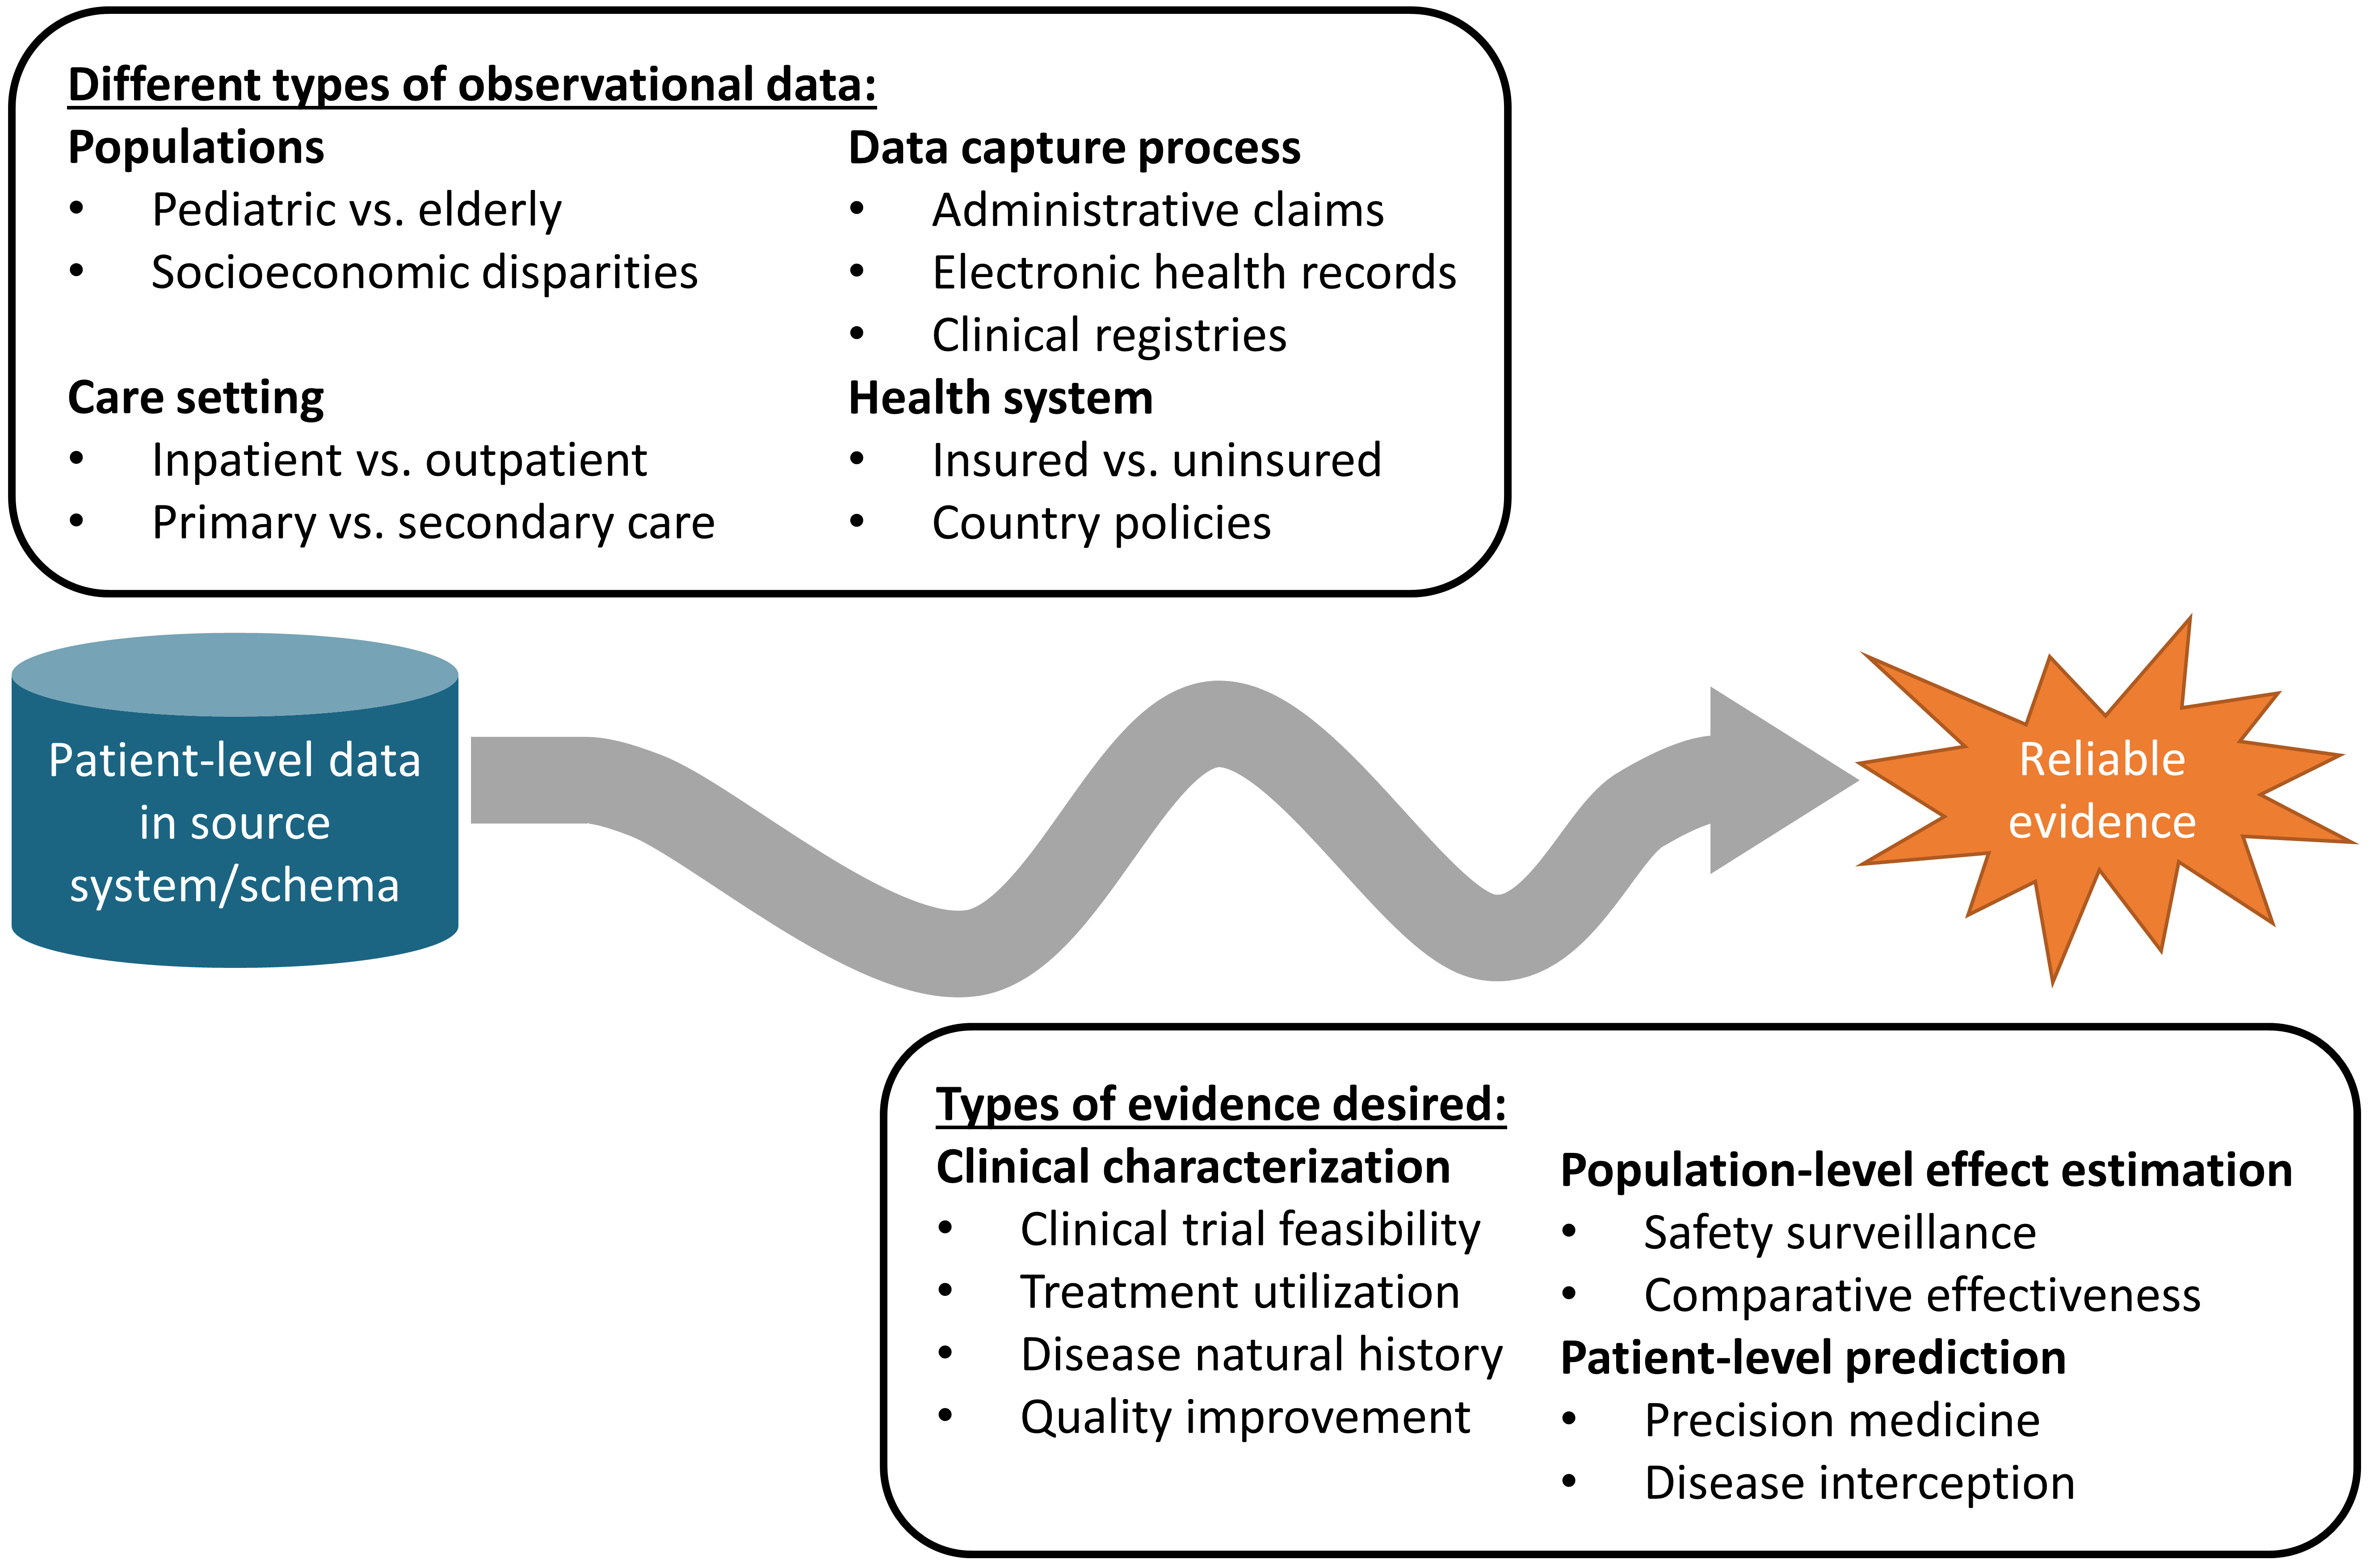
\includegraphics[width=1\linewidth]{images/OhdsiCommunity/datajourney} 

}

\caption{Le parcours des données à l'évidence}\label{fig:datajourney}
\end{figure}

Il existe différents types de bases de données observationnelles qui capturent des données disparates au niveau des patients dans les systèmes sources. Ces bases de données sont aussi diverses que le système de santé lui-même, reflétant différentes populations, contextes de soins et processus de capture de données. Il existe également différents types de preuves qui pourraient être utiles pour informer la prise de décision, qui peuvent être classifiées par les cas d'utilisation analytiques de la caractérisation clinique, de l'estimation des effets au niveau de la population et de la prédiction au niveau des patients. Indépendamment de l'origine (données sources) et de la destination souhaitée (preuve), le défi est encore compliqué par l'étendue des compétences cliniques, scientifiques et techniques requises pour entreprendre le parcours. Cela nécessite une compréhension approfondie de l'informatique de la santé, y compris la provenance complète des données sources depuis l'interaction au point de soins entre un patient et un fournisseur à travers les systèmes administratifs et cliniques et dans le référentiel final, avec une appréciation des biais qui peuvent survenir dans le cadre des politiques de santé et des incitations comportementales associées aux processus de capture et de conservation des données. Il nécessite une maîtrise des principes épidémiologiques et des méthodes statistiques pour traduire une question clinique en un design d'étude observationnelle convenablement adapté pour produire une réponse pertinente. Il nécessite les compétences techniques pour implémenter et exécuter des algorithmes de science des données performants sur des ensembles de données contenant des millions de patients avec des milliards d'observations cliniques sur des années de suivi longitudinal. Il nécessite des connaissances cliniques pour synthétiser ce qui a été appris à travers un réseau de données observationnelles avec des preuves provenant d'autres sources d'information, et pour déterminer comment cette nouvelle connaissance devrait impacter la politique de santé et la pratique clinique. En conséquence, il est assez rare qu'un seul individu possède les compétences et les ressources requises pour réussir seul le chemin des données à l'évidence. Au lieu de cela, le parcours nécessite souvent une collaboration entre plusieurs individus et organisations pour s'assurer que les meilleures données disponibles sont analysées en utilisant les méthodes les plus appropriées pour produire les preuves que toutes les parties prenantes peuvent avoir confiance et utiliser dans leurs processus de prise de décision.

\section{Observational Medical Outcomes Partnership}\label{observational-medical-outcomes-partnership}

Un exemple notable de collaboration en recherche observationnelle a été le partenariat Observational Medical Outcomes Partnership (OMOP). OMOP était un partenariat public-privé, présidé par la Food and Drug Administration des États-Unis, administré par la Fondation des Instituts Nationaux de la Santé, et financé par un consortium de compagnies pharmaceutiques qui ont collaboré avec des chercheurs universitaires et des partenaires de données de santé pour établir un programme de recherche visant à faire progresser la science de la surveillance active de la sécurité des produits médicaux en utilisant des données de santé observationnelle. \citep{stang2010omop} OMOP a établi une structure de gouvernance multipartite et conçu une série d'expériences méthodologiques pour tester empiriquement la performance de conceptions épidémiologiques alternatives et de méthodes statistiques lorsqu'elles sont appliquées à un ensemble de bases de données de réclamations administratives et de dossiers de santé électroniques pour identifier les véritables associations de sécurité des médicaments et les distinguer des faux positifs.

Reconnaissant les défis techniques de la conduite de recherches à travers des bases de données observationnelles disparates dans un environnement centralisé et un réseau de recherche distribué, l'équipe a conçu le Modèle de Données Commun OMOP (CDM) comme un mécanisme pour standardiser la structure, le contenu et la sémantique des données observationnelles et pour permettre d'écrire du code d'analyse statistique une fois qui pourrait être réutilisé sur chaque site de données. \citep{overhage2012cdm} Les expériences d'OMOP ont démontré qu'il était faisable d'établir un modèle de données commun et des vocabulaires standardisés qui pourraient accueillir différents types de données de divers contextes de soins et représentés par différents vocabulaires sources de manière à faciliter la collaboration interinstitutionnelle et les analyses performantes.

Dès le début, OMOP a adopté une approche de science ouverte, plaçant tous ses produits de travail, y compris les designs d'étude, les normes de données, le code d'analyse et les résultats empiriques, dans le domaine public pour promouvoir la transparence, renforcer la confiance dans la recherche que conduisait OMOP, mais aussi fournir une ressource communautaire qui pourrait être réutilisée pour avancer les objectifs de recherche des autres. Bien que le focus initial de l'OMOP ait été la sécurité des médicaments, le CDM OMOP a continuellement évolué pour soutenir un ensemble élargi de cas d'utilisation analytique, y compris l'efficacité comparative des interventions médicales et des politiques de système de santé.

Et bien qu'OMOP ait réussi à compléter ses expériences empiriques à grande échelle, \citep{ryan2012omop, ryan2013omop} développer des innovations méthodologiques, \citep{schuemie_2014} et générer des connaissances utiles qui ont informé l'utilisation appropriée des données observationnelles pour la prise de décision en matière de sécurité, \citep{madigan_2013, madigan2013design} l'héritage de l'OMOP peut être plus mémorable pour son adoption précoce des principes de la science ouverte et son stimulus qui a motivé la formation de la communauté OHDSI.

Lorsque le projet OMOP était terminé, ayant rempli son mandat de mener des recherches méthodologiques pour informer les activités de surveillance active de la FDA, l'équipe a reconnu que la fin du parcours OMOP devait devenir le début d'un nouveau parcours ensemble. Malgré la recherche méthodologique de l'OMOP fournissant des indications tangibles sur les meilleures pratiques scientifiques qui pourraient améliorer de manière démontrable la qualité des preuves générées à partir des données observationnelles, l'adoption de ces meilleures pratiques était lente. Plusieurs obstacles ont été identifiés, y compris : 1) des préoccupations fondamentales concernant la qualité des données observationnelles qui étaient considérées comme une priorité plus élevée à résoudre avant les innovations analytiques ; 2) une compréhension conceptuelle insuffisante des problèmes méthodologiques et des solutions ; 3) une incapacité à implémenter indépendamment des solutions dans leur environnement local ; 4) une incertitude quant à savoir si ces approches étaient applicables à leurs problèmes cliniques d'intérêt. Le fil conducteur commun à chaque obstacle était le sentiment qu'une personne seule n'avait pas tout ce dont elle avait besoin pour mettre en œuvre un changement par elle-même, mais avec un soutien collaboratif, tous les problèmes pouvaient être surmontés. Mais plusieurs domaines de collaboration étaient nécessaires :

\begin{itemize}
\tightlist
\item
  Collaboration pour établir des normes de données communautaires ouvertes, des vocabulaires standardisés et des conventions ETL (Extract-Transform-Load) qui augmenteraient la confiance dans la qualité des données sous-jacentes et promouvraient la cohérence dans la structure, le contenu et la sémantique pour permettre des analyses standardisées.
\item
  Collaboration pour la recherche méthodologique au-delà de la sécurité des médicaments pour établir des meilleures pratiques plus largement pour la caractérisation clinique, l'estimation des effets au niveau de la population et la prédiction au niveau des patients.
\item
  Collaboration pour le développement analytique open-source, pour codifier les meilleures pratiques scientifiques prouvées par la recherche méthodologique et les rendre accessibles sous forme d'outils disponibles publiquement qui peuvent être facilement adoptés par la communauté de recherche.
\item
  Collaboration pour des applications cliniques qui adressent des questions de santé importantes d'intérêt partagé à travers la communauté en naviguant collectivement le parcours des données à l'évidence.
\end{itemize}

De cette vision, OHDSI est née.
\#\# OHDSI en tant que Collaboratif de Science Ouverte

Observational Health Data Sciences and Informatics (OHDSI, prononcé ``Odyssey'') est une communauté de science ouverte qui vise à améliorer la santé en permettant à la communauté de générer de manière collaborative des preuves qui favorisent de meilleures décisions de santé et de meilleurs soins. \citep{Hripcsak2015} OHDSI mène des recherches méthodologiques pour établir les meilleures pratiques scientifiques pour l'utilisation appropriée des données de santé observationnelles, développe des logiciels d'analyse open-source qui codifient ces pratiques en solutions cohérentes, transparentes, et reproductibles, et applique ces outils et pratiques à des questions cliniques pour générer des preuves qui peuvent guider les politiques de santé et les soins aux patients.

\subsection{Notre Mission}\label{notre-mission}

\begin{quote}
Améliorer la santé en permettant à une communauté de générer de manière collaborative des preuves qui favorisent de meilleures décisions de santé et de meilleurs soins. \index{mission}
\end{quote}

\subsection{Notre Vision}\label{notre-vision}

\begin{quote}
Un monde dans lequel la recherche observationnelle produit une compréhension globale de la santé et des maladies. \index{vision}
\end{quote}

\subsection{Nos Objectifs}\label{nos-objectifs}

\begin{itemize}
\item
  \textbf{Innovation}: La recherche observationnelle est un domaine qui bénéficiera grandement d'une pensée disruptive. Nous recherchons activement et encourageons des approches méthodologiques novatrices dans notre travail.
\item
  \textbf{Reproductibilité}: Des preuves précises, reproductibles et bien calibrées sont nécessaires pour l'amélioration de la santé.
\item
  \textbf{Communauté}: Tout le monde est bienvenu pour participer activement à OHDSI, que vous soyez un patient, un professionnel de la santé, un chercheur, ou quelqu'un qui croit simplement en notre cause. \index{community}
\item
  \textbf{Collaboration}: Nous travaillons collectivement pour donner la priorité et répondre aux besoins réels des participants de notre communauté.
\item
  \textbf{Ouverture}: Nous nous efforçons de rendre toutes les activités de notre communauté ouvertes et accessibles au public, y compris les méthodes, outils et preuves que nous générons.
\item
  \textbf{Bienfaisance}: Nous cherchons à protéger les droits des individus et des organisations au sein de notre communauté en tout temps.
  \index{objectifs}
\end{itemize}

\section{Les Progrès de l'OHDSI}\label{les-progruxe8s-de-lohdsi}

OHDSI a grandi depuis sa création en 2014 pour inclure plus de 2 500 collaborateurs sur ses forums en ligne, représentant divers partenaires, y compris le milieu universitaire, l'industrie des produits médicaux, les régulateurs, les gouvernements, les payeurs, les fournisseurs de technologie, les systèmes de santé, les cliniciens, les patients, et différents domaines tels que l'informatique, l'épidémiologie, les statistiques, l'informatique biomédicale, les politiques de santé et les sciences cliniques. Une liste des collaborateurs OHDSI auto-identifiés est disponible sur le site Web de l'OHDSI. \footnote{\url{https://www.ohdsi.org/who-we-are/collaborators/}} La carte des collaborateurs OHDSI (Figure \ref{fig:collaboratormap}) met en lumière l'étendue et la diversité de la communauté internationale.

\begin{figure}

{\centering 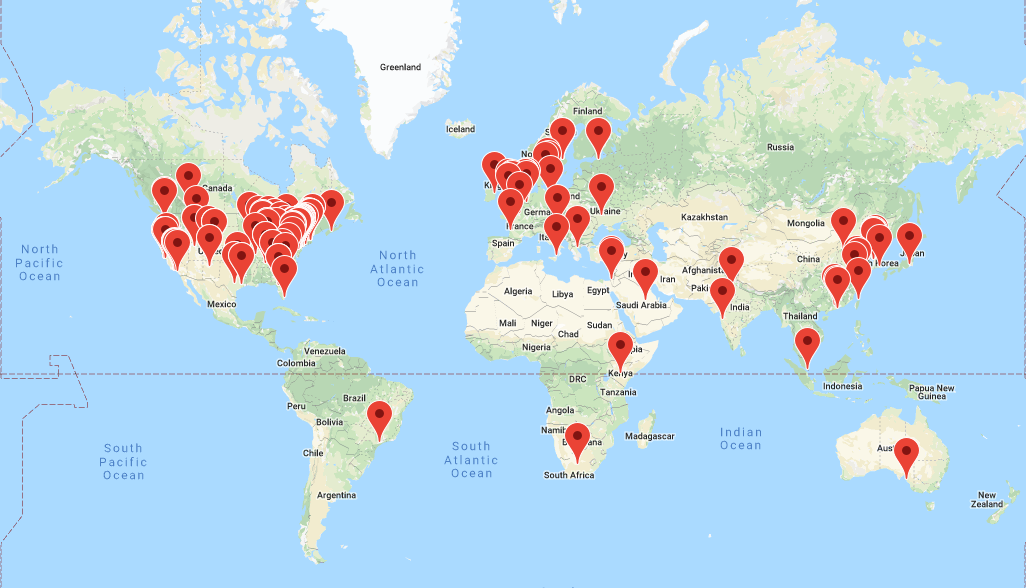
\includegraphics[width=1\linewidth]{images/OhdsiCommunity/mapOfCollaborators} 

}

\caption{Carte des collaborateurs OHDSI en août 2019}\label{fig:collaboratormap}
\end{figure}

En août 2019, OHDSI avait également établi un réseau de données de plus de 100 bases de données de soins de santé provenant de plus de 20 pays, capturant collectivement plus d'un milliard de dossiers de patients en utilisant une approche de réseau distribué appliquant une norme de données ouverte qu'elle maintient, le OMOP CDM. Un réseau distribué signifie que les données au niveau des patients ne sont pas obligées d'être partagées entre les individus ou les organisations. Au lieu de cela, les questions de recherche sont posées par les individus au sein de la communauté sous la forme d'un protocole d'étude accompagné d'un code d'analyse qui génère des preuves sous forme de statistiques sommaires agrégées, et seuls ces statistiques sommaires sont partagés entre les partenaires qui choisissent de collaborer à l'étude. Avec le réseau distribué OHDSI, chaque partenaire de données conserve une autonomie totale sur l'utilisation de leurs données au niveau des patients et continue d'observer les politiques de gouvernance des données au sein de leurs institutions respectives.

La communauté de développeurs OHDSI a créé une robuste bibliothèque d'outils analytiques open-source au-dessus de l'OMOP CDM pour soutenir trois cas d'utilisation : 1) la caractérisation clinique pour l'histoire naturelle des maladies, l'utilisation des traitements et l'amélioration de la qualité ; 2) l'estimation des effets au niveau de la population pour appliquer des méthodes d'inférence causale pour la surveillance de la sécurité des produits médicaux et l'efficacité comparative ; et 3) la prédiction au niveau des patients pour appliquer des algorithmes d'apprentissage automatique à la médecine de précision et à l'interception des maladies. Les développeurs d'OHDSI ont également développé des applications pour soutenir l'adoption de l'OMOP CDM, l'évaluation de la qualité des données et la facilitation des études de réseau OHDSI. Ces outils incluent des packages statistiques en arrière-plan construits en R et Python, et des applications web en front-end développées en HTML et Javascript. Tous les outils OHDSI sont open source et disponibles publiquement via Github. \footnote{\url{https://github.com/OHDSI}}

L'approche communautaire de science ouverte de l'OHDSI, couplée avec ses outils open-source, a permis des avancées considérables dans la recherche observationnelle. L'une des premières analyses de réseau OHDSI a examiné les parcours de traitement à travers trois maladies chroniques : le diabète, la dépression et l'hypertension. Publiée dans les Actes de l'Académie Nationale des Sciences, c'était l'une des plus grandes études observationnelles jamais menées, avec des résultats provenant de 11 sources de données couvrant plus de 250 millions de patients, et a révélé de grandes différences géographiques et une hétérogénéité des patients dans les choix de traitement qui n'avaient jamais été observables auparavant. \citep{Hripcsak7329} OHDSI a développé de nouvelles méthodes statistiques de correction du biais de confusion \citep{tian_2018} et d'évaluation de la validité des preuves observationnelles pour l'inférence causale, \citep{schuemie_2018} et a appliqué ces approches dans de multiples contextes, allant d'une question de surveillance de la sécurité individuelle dans l'épilepsie \citep{duke_2017} à l'efficacité comparative des médicaments de deuxième ligne pour le diabète \citep{vashisht_2018} jusqu'à une étude à grande échelle d'estimation des effets au niveau de la population pour la sécurité comparative des traitements de la dépression. \citep{schuemie_2018b} La communauté OHDSI a également établi un cadre pour comment appliquer de manière responsable les algorithmes d'apprentissage automatique aux données de santé observationnelles, \citep{reps2018} qui a été appliqué dans divers domaines thérapeutiques. \citetext{\citealp[ ]{johnston_2019}; \citealp[ ]{cepeda_2018}; \citealp{reps_2019}}

\section{Collaborer avec OHDSI}\label{collaborer-avec-ohdsi}

Puisque OHDSI est une communauté visant à favoriser la collaboration pour générer des preuves, qu'est-ce que cela signifie d'être un collaborateur OHDSI ? Si vous êtes quelqu'un qui croit en la mission de l'OHDSI et qui est intéressé à apporter une contribution à n'importe quelle étape du parcours allant des données aux preuves, alors OHDSI peut être la communauté pour vous. Les collaborateurs peuvent être des individus qui ont accès à des données au niveau des patients et souhaitent voir ces données utilisées pour générer des preuves. Les collaborateurs peuvent être des méthodologistes intéressés par l'établissement des meilleures pratiques scientifiques et l'évaluation d'approches alternatives. Les collaborateurs peuvent être des développeurs de logiciels intéressés à appliquer leurs compétences en programmation pour créer des outils utilisables par le reste de la communauté. Les collaborateurs peuvent être des chercheurs cliniques ayant des questions importantes de santé publique et cherchant à fournir des preuves à ces questions à la communauté de la santé au sens large par le biais de publications et d'autres formes de diffusion. Les collaborateurs peuvent être des individus ou des organisations qui croient en cette cause commune pour la santé publique et souhaitent fournir des ressources pour assurer que la communauté puisse se maintenir et continuer sa mission, y compris en organisant des activités communautaires et des sessions de formation à travers le monde. Peu importe votre discipline ou votre affiliation, OHDSI cherche à être un lieu où les individus peuvent travailler ensemble vers un objectif commun, chacun apportant sa contribution individuelle qui, collectivement, peut faire avancer les soins de santé. Si vous êtes intéressé à rejoindre le voyage, consultez le chapitre \ref{WhereToBegin} (``Par Où Commencer'') pour savoir comment débuter.

\section{Résumé}\label{ruxe9sumuxe9}

\begin{rmdsummary}
\begin{itemize}
\item
  La mission de l'OHDSI est d'améliorer la santé en permettant à une communauté de générer de manière collaborative des preuves qui favorisent de meilleures décisions de santé et de meilleurs soins.
\item
  Notre vision est un monde dans lequel la recherche observationnelle produit une compréhension globale de la santé et des maladies, ce qui sera atteint par nos objectifs d'innovation, de reproductibilité, de communauté, de collaboration, d'ouverture et de bienfaisance.
\item
  Les collaborateurs de l'OHDSI sont concentrés sur les normes de données de la communauté ouverte, la recherche méthodologique, le développement d'analyses open-source, et les applications cliniques pour améliorer le parcours allant des données aux preuves.
\end{itemize}
\end{rmdsummary}

\chapter{Par où commencer}\label{WhereToBegin}

\emph{Responsables du chapitre : Hamed Abedtash \& Kristin Kostka}

\begin{quote}
``Un voyage de mille lieues commence par un seul pas.'' - Lao Tzu
\end{quote}

La communauté OHDSI représente une mosaïque de parties prenantes à travers le milieu académique, l'industrie et les entités gouvernementales. Notre travail bénéficie à une gamme d'individus et d'organisations, y compris les patients, les prestataires et les chercheurs, ainsi que les systèmes de santé, l'industrie et les agences gouvernementales. Ce bénéfice est réalisé en améliorant à la fois la qualité des analyses de données de santé et l'utilité des données de santé pour ces parties prenantes. Nous croyons que la recherche observationnelle est un domaine qui tire grand profit de la pensée disruptive. Nous recherchons activement et encourageons de nouvelles approches méthodologiques dans notre travail. \index{community}
\#\# Rejoignez le voyage
Tout le monde est invité à participer activement à OHDSI, que vous soyez patient, professionnel de la santé, chercheur ou simplement quelqu'un qui croit en notre cause. OHDSI maintient un modèle d'adhésion inclusif. Devenir collaborateur OHDSI ne nécessite aucun frais d'adhésion. La collaboration est aussi simple que lever la main pour être inclus dans le décompte annuel des membres d'OHDSI. L'engagement est totalement volontaire. Un collaborateur peut avoir n'importe quel niveau de contribution au sein de la communauté, allant de la participation aux appels hebdomadaires de la communauté à la direction d'études de réseau ou de groupes de travail OHDSI. Les collaborateurs n'ont pas besoin d'être détenteurs de données pour être considérés comme des membres actifs de la communauté. La communauté OHDSI vise à servir les détenteurs de données, les chercheurs, les prestataires de soins de santé ainsi que les patients et consommateurs. Un registre des profils des collaborateurs est maintenu et périodiquement mis à jour sur le site web d'OHDSI. L'adhésion est encouragée via les appels communautaires OHDSI, les groupes de travail et les chapitres régionaux.\index{join the journey} \index{workgroups} \index{chapters}

\begin{figure}

{\centering 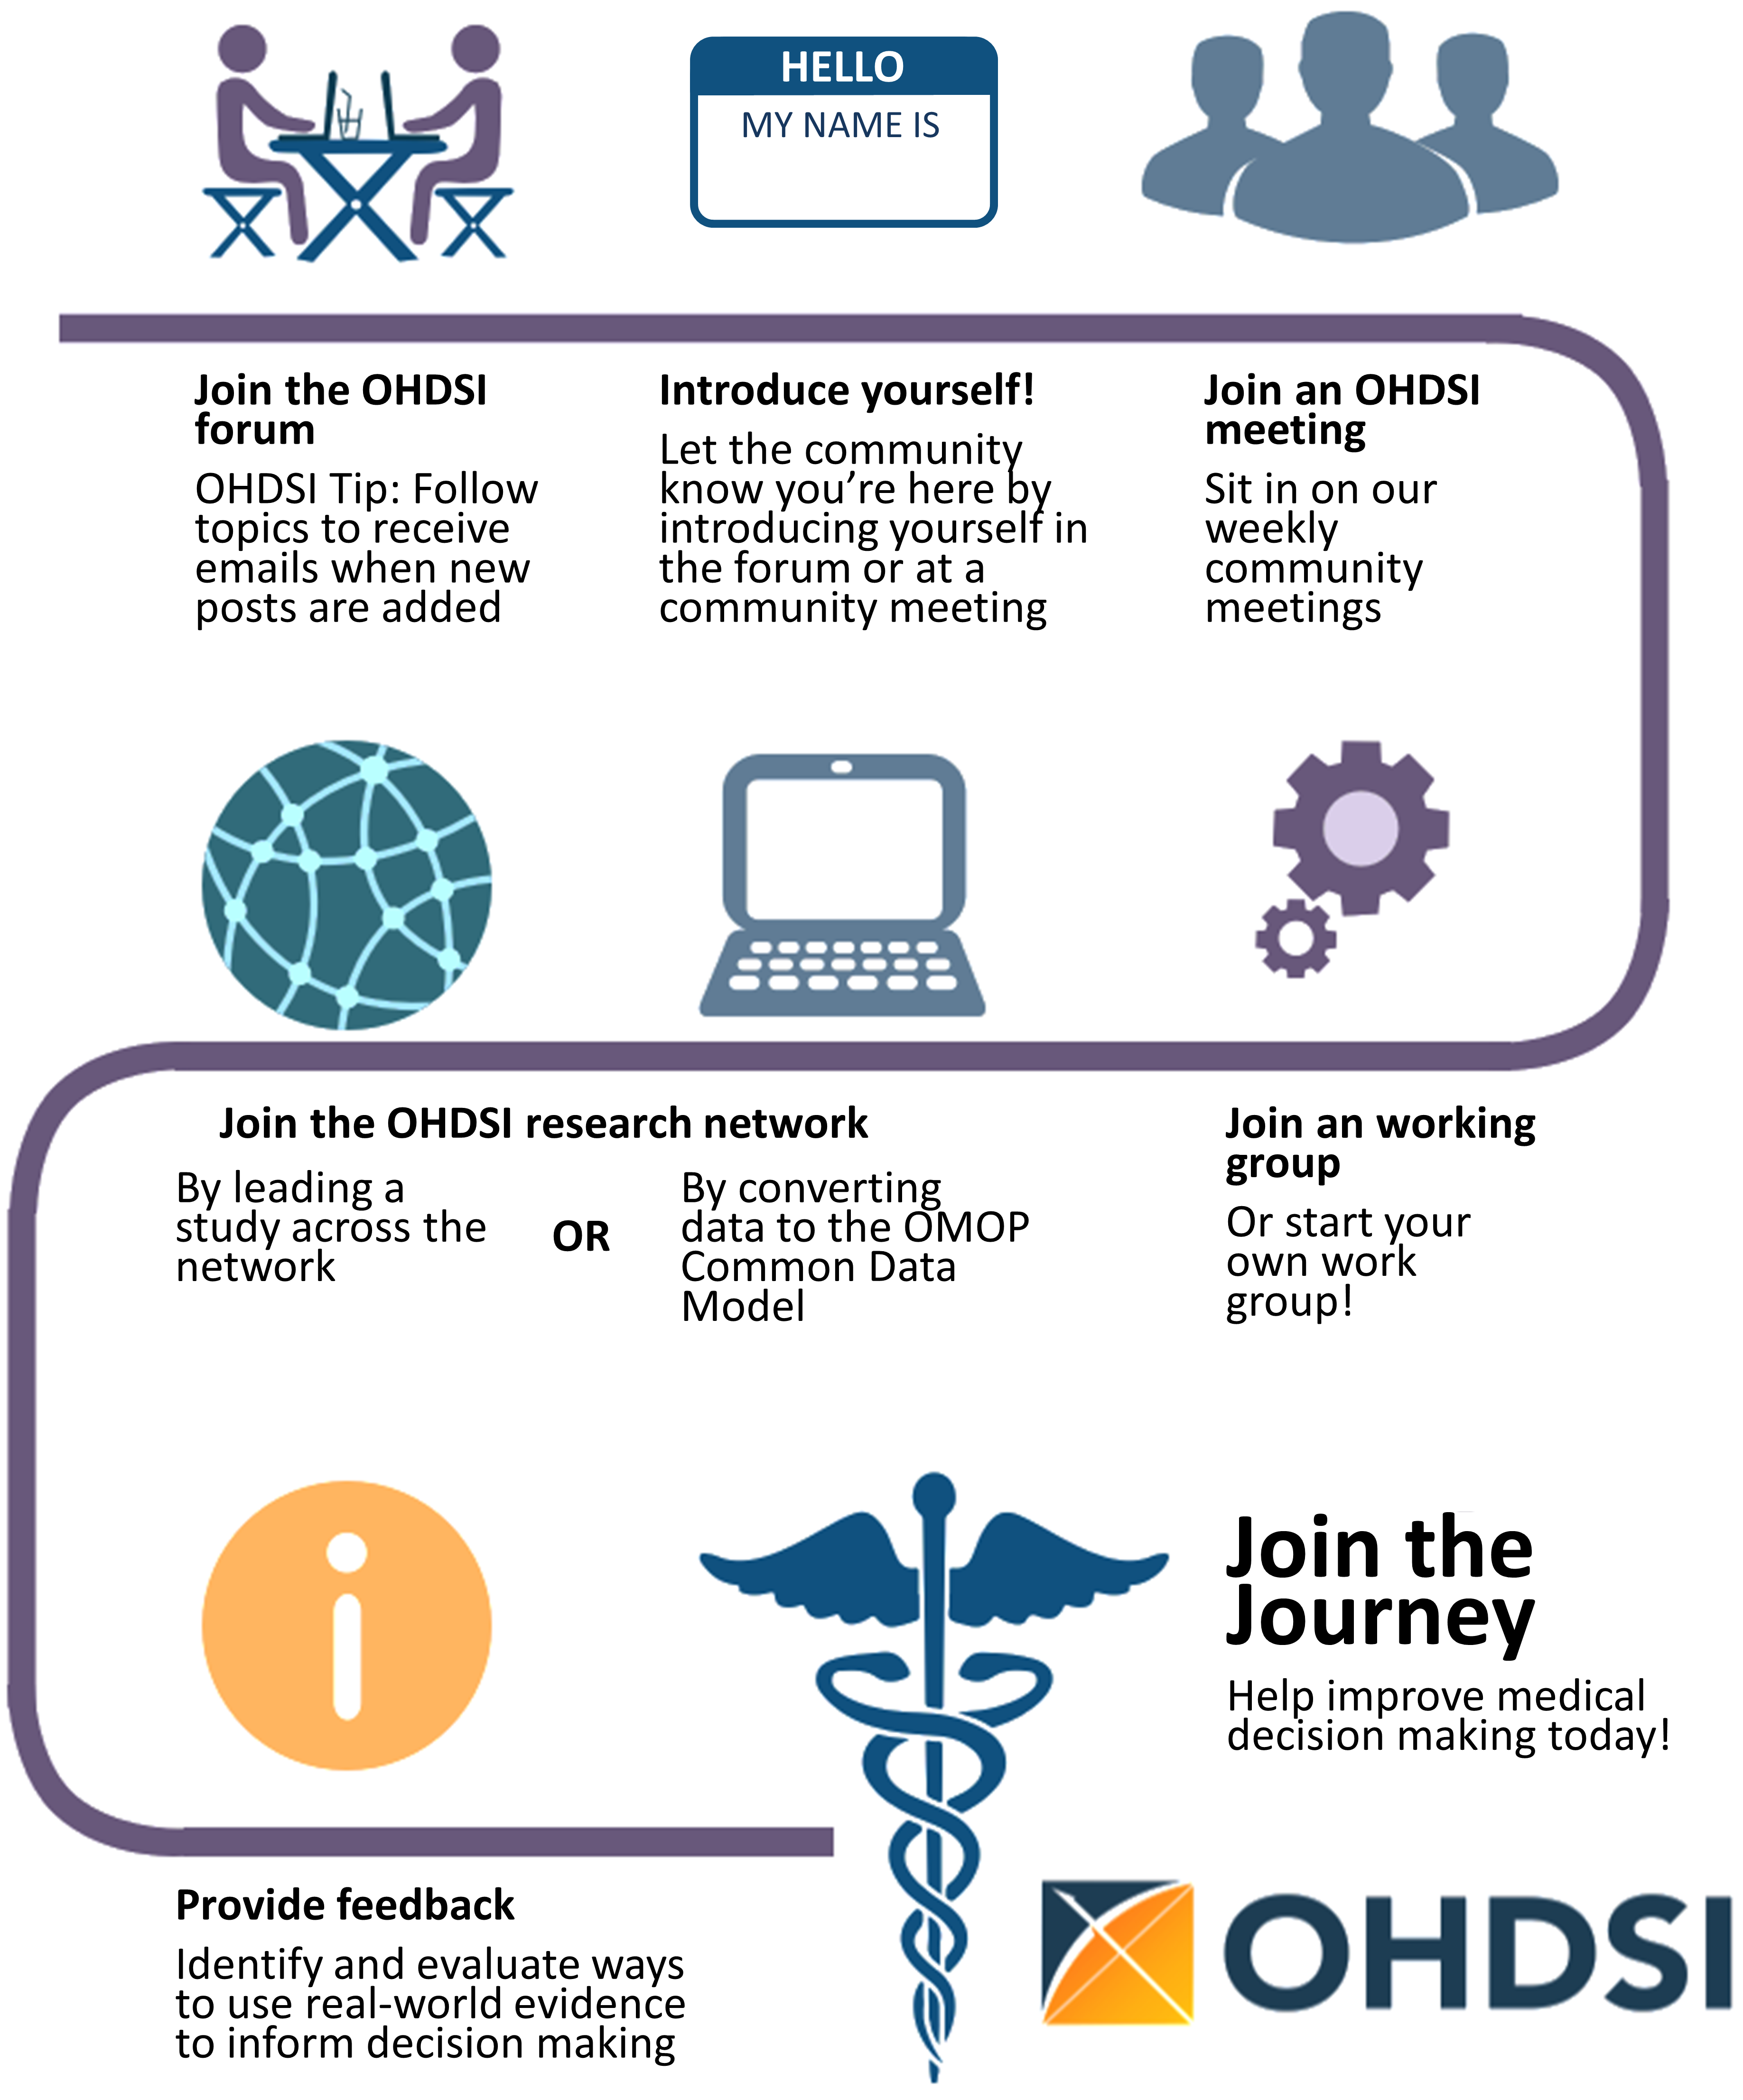
\includegraphics[width=0.9\linewidth]{images/WhereToBegin/joinTheJourney} 

}

\caption{Rejoignez le voyage - Comment devenir collaborateur OHDSI.}\label{fig:jointhejourney}
\end{figure}

\subsection{Forums OHDSI}\label{forums-ohdsi}

Le forum OHDSI\footnote{\url{https://forums.ohdsi.org}} est un site de discussion en ligne où les collaborateurs de la communauté OHDSI peuvent tenir des conversations sous forme de messages postés. Le forum se compose d'une structure répertoire en arbre. Le niveau supérieur est ``Catégories''. Les forums peuvent être divisés en catégories pour les discussions pertinentes. Sous les catégories se trouvent des sous-forums et ces sous-forums peuvent avoir d'autres sous-forums. Les sujets (couramment appelés fils de discussion) se trouvent sous le niveau le plus bas des sous-forums et c'est là que les membres des forums peuvent lancer leurs discussions ou posts.

Dans les forums OHDSI, vous pouvez trouver des catégories de contenu incluant :

\begin{itemize}
\tightlist
\item
  \textbf{Général :} pour des discussions générales sur la communauté OHDSI et comment s'impliquer
\item
  \textbf{Implémenteurs :} pour discuter de la mise en œuvre du Modèle de Données Commun et du cadre analytique OHDSI dans votre environnement local
\item
  \textbf{Développeurs :} pour discuter du développement open-source d'applications OHDSI et d'autres outils utilisant le CDM OMOP
\item
  \textbf{Chercheurs :} pour discuter de la recherche basée sur le CDM, y compris la génération de preuves, la recherche collaborative, les méthodes statistiques et autres sujets d'intérêt pour le Réseau de Recherche OHDSI
\item
  \textbf{Constructeurs de CDM :} pour discuter du développement en cours du CDM, y compris les exigences, le vocabulaire et les aspects techniques
\item
  \textbf{Utilisateurs de vocabulaire :} pour discuter du contenu du vocabulaire
\item
  \textbf{Chapitres régionaux (par exemple, Corée, Chine, Europe) :} pour des discussions régionales dans leurs langues natales liées aux implémentations locales d'OMOP et aux activités de la communauté OHDSI
\end{itemize}

Pour commencer à poster vos propres sujets, vous devrez vous inscrire pour un compte. Une fois que vous avez un compte sur le forum, il est encouragé de vous présenter dans le Sujet Général sous le fil de discussion appelé ``Bienvenue chez OHDSI! - Merci de vous présenter''. Vous êtes invités à répondre et 1) À vous présenter et nous dire un peu ce que vous faites et 2) À nous faire savoir comment vous aimeriez aider dans la communauté (ex. développement de logiciels, exécution d'études, rédaction de documents de recherche, etc.). Maintenant, vous êtes sur votre chemin OHDSI! À partir de là, vous êtes encouragés à participer aux discussions. La Communauté OHDSI encourage l'utilisation des Forums comme moyen de poser des questions, de discuter de nouvelles idées et de collaborer. \index{forum}

\begin{rmdimportant}
Vous pouvez sélectionner des sujets à ``suivre''. Cela signifie que chaque fois qu'un nouveau post est ajouté dans un sujet que vous suivez, vous recevrez un e-mail et pourrez répondre directement au post via votre e-mail. Suivez le fil général pour recevoir des détails sur les prochains ordres du jour des réunions, les opportunités de collaboration et recevez le digest hebdomadaire OHDSI directement dans votre boîte de réception!
\end{rmdimportant}

\subsection{Événements OHDSI}\label{uxe9vuxe9nements-ohdsi}

OHDSI organise régulièrement des événements en personne pour offrir aux collaborateurs des opportunités d'apprendre les uns des autres et de se connecter pour favoriser de futures collaborations. Ces événements sont communiqués sur le site Web d'OHDSI et sont gratuits pour toute personne intéressée à y assister.

Les symposiums OHDSI sont des conférences scientifiques organisées annuellement aux États-Unis, en Europe et en Asie, où les collaborateurs peuvent présenter leurs dernières recherches par des conférences plénières, des présentations de posters et des démonstrations de logiciels. Les symposiums OHDSI offrent un excellent lieu de réseautage et d'apprentissage des progrès les plus récents au sein de la communauté. Les symposiums OHDSI sont généralement accompagnés de tutoriels OHDSI, enseignés par des collaborateurs OHDSI en tant que professeurs du cours, qui offrent aux nouveaux membres de la communauté l'opportunité de s'engager de manière pratique sur des sujets autour des standards de données et des meilleures pratiques d'analyse. Ces tutoriels sont généralement enregistrés en vidéo et mis à disposition sur le site Web OHDSI après les événements pour ceux qui ne peuvent pas y assister en personne.

Les événements face-à-face des collaborateurs OHDSI sont des forums plus restreints centrés sur un problème d'intérêt commun à aborder pendant le temps passé ensemble. Les événements passés ont inclus un hackathon de phénotype, un hackathon de qualité des données et un hackathon de documentation de logiciels open-source. OHDSI a organisé plusieurs événements Study-a-thon, où l'objectif de la session de plusieurs jours est de collaborer en équipe sur une question de recherche particulière en concevant et en mettant en œuvre une analyse observationnelle appropriée, en exécutant l'étude à travers le réseau OHDSI et en synthétisant les preuves pour une diffusion publique. Dans tous ces événements, il y a un désir commun de résoudre un problème commun mais aussi un intérêt partagé pour fournir un environnement accueillant qui encourage l'apprentissage et l'amélioration continue du processus de résolution collaborative de problèmes.

Découvrez la puissance de la Communauté OHDSI. Explorez les anciens symposiums, les réunions en face-à-face et regardez les tutoriels OHDSI en visitant la section \href{https://www.ohdsi.org/past-events/}{Événements passés OHDSI} sur le site Web d'OHDSI. Les événements passés sont mis à jour régulièrement pour archiver les événements de la communauté.

\subsection{Appels de la communauté OHDSI}\label{appels-de-la-communautuxe9-ohdsi}

Les appels de la communauté OHDSI sont une opportunité hebdomadaire de mettre en lumière l'activité en cours au sein de la communauté OHDSI. Tenus chaque mardi de 11h à 12h ET, ces téléconférences sont un moment pour la communauté OHDSI de se réunir pour partager les développements récents et reconnaître les accomplissements des collaborateurs individuels, des groupes de travail et de la communauté dans son ensemble. La réunion de chaque semaine est enregistrée et les présentations sont archivées dans les ressources du site Web OHDSI.

Tous les collaborateurs OHDSI sont invités à participer à cette téléconférence hebdomadaire et encouragés à proposer des sujets pour les discussions communautaires. Les appels communautaires OHDSI peuvent être un forum pour partager des résultats de recherche, présenter et recueillir des commentaires sur les travaux en cours, démontrer des outils logiciels open-source en cours de développement, débattre des meilleures pratiques communautaires pour la modélisation des données et les analyses, et brainstormer sur de futures opportunités de collaboration pour les subventions/publications/ateliers de conférence. Si vous êtes un collaborateur avec un sujet pour une prochaine réunion des collaborateurs OHDSI, vous êtes invités à poster vos pensées sur les forums OHDSI.

En tant que nouveau membre de la communauté OHDSI, il est encouragé d'ajouter cette série d'appels à votre calendrier pour vous familiariser avec ce qui se passe dans tout le réseau OHDSI. Si vous souhaitez rejoindre un appel OHDSI, veuillez consulter les \href{https://forums.ohdsi.org/}{Forums OHDSI} pour les annonces. Les sujets des appels communautaires varient d'une semaine à l'autre. Vous pouvez également consulter le digest hebdomadaire OHDSI sur le forum OHDSI pour plus d'informations sur les sujets de présentation hebdomadaires. Les nouveaux arrivants sont invités à se présenter lors de leur premier appel et à parler à la communauté d'eux-mêmes, de leur parcours et de ce qui les a amenés à OHDSI. \index{community!community calls}

\subsection{Groupes de travail OHDSI}\label{groupes-de-travail-ohdsi}

OHDSI a une variété de projets en cours dirigés par des équipes de groupes de travail. Chaque groupe de travail a son propre groupe de direction qui détermine les objectifs, les buts et les artefacts du projet à contribuer à la communauté. La participation aux groupes de travail est ouverte à tous ceux qui ont un intérêt à contribuer aux objectifs et buts du projet. Les groupes de travail peuvent être des objectifs stratégiques à long terme ou des projets à court terme pour atteindre un besoin spécifique dans la communauté. La cadence des réunions des groupes de travail est déterminée par les dirigeants du projet et variera d'un groupe à l'autre. Une liste des groupes de travail actifs est maintenue sur le \href{https://www.ohdsi.org/web/wiki/doku.php?id=projects:overview}{Wiki OHDSI}. \index{workgroups}

Le tableau \ref{tab:OHDSIworkgroups} fournit une référence rapide aux groupes de travail OHDSI actifs. Vous êtes encouragés à rejoindre un appel et à en savoir plus.

\begin{longtable}[]{@{}
  >{\raggedright\arraybackslash}p{(\columnwidth - 4\tabcolsep) * \real{0.1471}}
  >{\raggedright\arraybackslash}p{(\columnwidth - 4\tabcolsep) * \real{0.5588}}
  >{\raggedright\arraybackslash}p{(\columnwidth - 4\tabcolsep) * \real{0.2941}}@{}}
\caption{\label{tab:OHDSIworkgroups} Groupes de travail OHDSI notables}\tabularnewline
\toprule\noalign{}
\begin{minipage}[b]{\linewidth}\raggedright
Nom du groupe de travail
\end{minipage} & \begin{minipage}[b]{\linewidth}\raggedright
Objectif
\end{minipage} & \begin{minipage}[b]{\linewidth}\raggedright
Public cible
\end{minipage} \\
\midrule\noalign{}
\endfirsthead
\toprule\noalign{}
\begin{minipage}[b]{\linewidth}\raggedright
Nom du groupe de travail
\end{minipage} & \begin{minipage}[b]{\linewidth}\raggedright
Objectif
\end{minipage} & \begin{minipage}[b]{\linewidth}\raggedright
Public cible
\end{minipage} \\
\midrule\noalign{}
\endhead
\bottomrule\noalign{}
\endlastfoot
Atlas \& WebAPI & Atlas et WebAPI font partie de l'architecture logicielle open-source OHDSI qui vise à fournir des capacités analytiques standardisées basées sur la fondation du Modèle de Données Commun OMOP. & Développeurs de logiciels Java et JavaScript visant à améliorer et contribuer à la plateforme open-source Atlas/WebAPI \\
CDM \& Vocabulaire & Continuer à développer le Modèle de Données Commun OMOP dans le but d'analyses systématiques, standardisées et à grande échelle appliquées aux données cliniques des patients. Améliorer la qualité des Vocabulaires Standardisés en augmentant leur couverture des systèmes de codage internationaux et des aspects cliniques des soins aux patients afin de soutenir les analyses standardisées développées par d'autres groupes de travail. & Toute personne ayant un intérêt à améliorer le Modèle de Données Commun OMOP et les Vocabulaires Standardisés pour répondre à tous les besoins et cas d'utilisation \\
Génomique & Étendre le CDM OMOP pour incorporer les données génomiques des patients. Le groupe définira un schéma compatible avec le CDM qui pourra stocker des informations sur les variantes génétiques provenant de divers processus de séquençage. & Ouvert à tous \\
Estimation au niveau de la population & Développer des méthodes scientifiques pour la recherche observationnelle menant à des estimations des effets au niveau de la population qui soient précises, fiables et reproductibles, et faciliter l'utilisation de ces méthodes par la communauté. & Ouvert à tous \\
Traitement du Langage Naturel & Promouvoir l'utilisation des informations textuelles des dossiers de santé électroniques (DSE) pour les études observationnelles sous l'égide d'OHDSI. Pour faciliter cet objectif, le groupe développera des méthodes et des logiciels qui pourront être mis en œuvre pour utiliser le texte clinique pour les études de la communauté OHDSI. & Ouvert à tous \\
Prédiction au niveau des patients & Établir un processus standardisé pour développer des modèles de prédiction centrés sur le patient qui soient précis et bien calibrés et puissent être utilisés pour plusieurs résultats d'intérêt et appliqués aux données de soins observables de toute sous-population de patients d'intérêt & Ouvert à tous \\
Bibliothèque de phénotypes de référence & Permettre aux membres de la communauté OHDSI de trouver, évaluer et utiliser des définitions de cohortes validées par la communauté pour la recherche et d'autres activités & Ouvert à tous ceux qui s'intéressent à la curation et à la validation des phénotypes \\
Groupe de travail FHIR & Établir la feuille de route pour l'intégration OHDSI FHIR et faire des recommandations à la communauté plus large concernant l'utilisation de l'implémentation FHIR et des données dans la communauté des DSE pour les études observationnelles basées sur OHDSI et pour la diffusion des données et des résultats de recherche OHDSI via les outils et API basés sur FHIR. & Ouvert à tous ceux qui s'intéressent à l'interopérabilité \\
SIG & Étendre le CDM OMOP et utiliser les outils OHDSI afin que les historiques d'exposition environnementale des patients puissent être liés à leurs phénotypes cliniques & Ouvert à tous ceux qui s'intéressent aux attributs géographiques liés à la santé \\
Essais cliniques & Comprendre les cas d'utilisation des essais cliniques où la plateforme et l'écosystème OHDSI peuvent aider les essais à tout aspect, et contribuer à la mise à jour des outils OHDSI pour soutenir. & Ouvert à tous ceux qui s'intéressent aux essais cliniques \\
THEMIS & L'objectif de THEMIS est de développer des conventions standard, au-delà des conventions du CDM OMOP, pour garantir que les protocoles ETL conçus sur chaque site OMOP soient de la plus haute qualité, reproductibles et efficaces. & Ouvert à tous ceux qui s'intéressent à la standardisation ETL \\
Métadonnées \& Annotations & Notre objectif est de définir un processus standard pour stocker des métadonnées et des annotations rédigées par des humains et des machines dans le Modèle de Données Commun afin de s'assurer que les chercheurs peuvent consommer et créer des artefacts de données utiles sur les ensembles de données observationnelles. & Ouvert à tous \\
Données de santé générées par les patients (PGHD) & L'objectif de ce GT est de développer des conventions ETL, un processus d'intégration avec les données cliniques et un processus analytique pour les PGHD, qui sont générées par des téléphones intelligents/appareils/appareils portables. & Ouvert à tous \\
Femmes d'OHDSI & Fournir un forum pour les femmes au sein de la communauté OHDSI pour se réunir et discuter des défis qu'elles rencontrent en tant que femmes travaillant dans les domaines des sciences, de la technologie, de l'ingénierie et des mathématiques (STEM). Nous visons à faciliter des discussions où les femmes peuvent partager leurs perspectives, soulever des préoccupations, proposer des idées sur la façon dont la communauté OHDSI peut soutenir les femmes dans les STEM, et inspirer les femmes à devenir des leaders au sein de la communauté et de leurs domaines respectifs. & Ouvert à toutes celles qui se reconnaissent dans cette mission \\
Comité de pilotage & Maintenir la mission, la vision et les valeurs d'OHDSI en s'assurant que toutes les activités et événements OHDSI sont alignés sur les besoins de notre communauté en croissance. De plus, le groupe sert de groupe consultatif pour le centre de coordination OHDSI basé à Columbia en fournissant des conseils sur la direction future d'OHDSI. & Leaders au sein de la communauté \\
\end{longtable}

\subsection{Chapitres régionaux OHDSI}\label{chapitres-ruxe9gionaux-ohdsi}

Un chapitre régional OHDSI représente un groupe de collaborateurs OHDSI situés dans une zone géographique qui souhaitent organiser des événements de réseautage locaux et des réunions pour aborder des problèmes spécifiques à leur localisation géographique. Aujourd'hui, les chapitres régionaux OHDSI incluent OHDSI en Europe\footnote{\url{https://www.ohdsi-europe.org/}}, OHDSI en Corée du Sud\footnote{\url{https://forums.ohdsi.org/c/For-collaborators-wishing-to-communicate-in-Korean}} et OHDSI en Chine.\footnote{\url{https://ohdsichina.org/}} Si vous souhaitez créer un chapitre régional OHDSI dans votre région, vous pouvez le faire en suivant le processus de chapitre régional OHDSI décrit sur le \href{https://www.ohdsi.org/who-we-are/regional-chapters}{site web OHDSI}. \index{chapters}

\subsection{Réseau de recherche OHDSI}\label{ruxe9seau-de-recherche-ohdsi}

De nombreux collaborateurs OHDSI sont intéressés par la conversion de leurs données au Modèle de Données Commun OMOP. Le réseau de recherche OHDSI représente une communauté diversifiée et mondiale de bases de données observationnelles qui ont subi des processus d'Extraction-Tranform-Load (ETL) pour devenir conformes au modèle OMOP. Si votre parcours dans la communauté OHDSI inclut la transformation de données, de nombreuses ressources communautaires sont disponibles pour vous aider, y compris des tutoriels sur le CDM OMOP et les Vocabulaires, des outils gratuits pour aider à la conversion et des groupes de travail ciblant des domaines spécifiques ou des types de conversions de données. Les collaborateurs OHDSI sont encouragés à utiliser le forum OHDSI pour discuter et résoudre les défis qui surviennent pendant les conversions CDM.
\#\# Où vous situez-vous
À ce stade, vous vous demandez peut-être : \emph{où me situe-je dans la communauté OHDSI ?}

\textbf{Je suis un chercheur clinique cherchant à démarrer une étude.} Si vous êtes un chercheur clinique intéressé par l'utilisation du réseau de recherche OHDSI pour répondre à une question spécifique -- peut-être même publier un article -- vous êtes au bon endroit. Vous pouvez commencer par poster votre idée sur le \href{https://forums.ohdsi.org/c/researchers}{Sujet des chercheurs OHDSI} sur le forum OHDSI. Cela vous aidera à vous connecter avec des chercheurs ayant des intérêts similaires. OHDSI aime publier et dispose de nombreuses ressources pour accélérer la transformation de votre question de recherche en une analyse et un article. Vous pouvez trouver plus d'informations dans les chapitres \ref{Characterization}, \ref{PopulationLevelEstimation} et \ref{PatientLevelPrediction}.

\textbf{Je veux lire et consommer les informations produites par la communauté OHDSI.} Que vous soyez un patient, un clinicien en exercice ou un expert en la matière dans le domaine de la santé, OHDSI souhaite vous fournir des preuves de haute qualité pour vous aider à mieux comprendre les résultats de santé. Peut-être que cela fait un moment que vous n'avez pas écrit de code. Peut-être que vous n'avez jamais programmé. Vous avez une place dans cette communauté. Nous vous appelons un \emph{consommateur de preuves} -- vous êtes les personnes qui transforment la recherche OHDSI en action. Vous examinez pour savoir quelles preuves OHDSI a générées et génère, souhaitant peut-être également suggérer des questions pertinentes pour vous. Nous vous invitons à rejoindre la discussion. Commencez à poser des questions sur le \href{http://forums.ohdsi.org}{Forum OHDSI}. Assistez aux appels communautaires et découvrez les dernières recherches. Assistez aux symposiums et aux réunions en face à face de l'OHDSI pour vous engager directement avec la communauté. Vos questions sont une partie importante de la communauté OHDSI. Prenez la parole et aidez-nous à en apprendre davantage sur les preuves que vous recherchez !

\textbf{Je travaille dans un rôle de leadership en santé. Je peux être un propriétaire de données et/ou représenter un. J'évalue l'utilité du CDM OMOP et des outils analytiques OHDSI pour mon organisation.} En tant qu'administrateur/leader d'une organisation, vous avez peut-être entendu parler d'OHDSI et vous vous demandez si le CDM OMOP pourrait fonctionner pour vos cas d'utilisation. Vous pouvez commencer par regarder les matériaux des \href{https://www.ohdsi.org/past-events/}{Événements passés d'OHDSI} pour voir le corpus de recherche. Vous pouvez rejoindre un appel communautaire et simplement écouter. Vous pouvez également trouver que le chapitre \ref{DataAnalyticsUseCases} (Cas d'utilisation de l'analyse de données) vous aide à comprendre le type de recherche que les outils analytiques CDM OMOP et OHDSI peuvent permettre. La communauté OHDSI est là pour vous accompagner tout au long de votre parcours. N'ayez pas peur de prendre la parole et de demander des exemples si vous avez des domaines spécifiques qui vous intéressent. Plus de 200 organisations dans le monde collaborent avec OHDSI, il y a de nombreuses histoires de succès pour démontrer la valeur de cette communauté.

\textbf{Je suis un administrateur de base de données cherchant à ETL/converter les données de mon institution au CDM OMOP.} Choisir de ``OMOP'' vos données est une entreprise novatrice et utile. Si vous débutez dans votre processus ETL, consultez les \href{https://www.ohdsi-europe.org/images/symposium-2019/tutorials/OHDSI_Vocabulary_CDM_Tutorial.pdf}{Diapositives du tutoriel ETL de la communauté OHDSI} ou inscrivez-vous pour la prochaine session lors d'un symposium OHDSI à venir. Envisagez de participer aux appels du groupe de travail THEMIS et de vous engager sur le forum OHDSI avec vos questions. Vous trouverez une mine de connaissances dans la communauté intéressée à aider votre mise en œuvre réussie du CDM OMOP. Ne soyez pas timide!

\textbf{Je suis un biostatisticien et/ou un développeur de méthodes intéressé à contribuer à la pile d'outils OHDSI.} Vous êtes doué en R. Vous savez comment faire un commit sur Git. Surtout, vous êtes impatient d'apporter votre expertise à la bibliothèque de méthodes OHDSI et de développer davantage ces méthodologies. Vous voudrez commencer par rejoindre les appels des groupes de travail sur l'estimation au niveau de la population ou la prédiction au niveau du patient pour en savoir plus sur les priorités actuelles de la communauté. Lorsque vous utilisez les outils OHDSI, vous pouvez également signaler des problèmes sous le dépôt GitHub correspondant (par exemple, s'il s'agit d'un problème lié au package SQL Render, vous déposeriez sous le dépôt GitHub de OHDSI/SqlRender). Nous accueillons vos contributions !

\textbf{Je suis un développeur de logiciels intéressé à construire un outil qui complète la pile d'outils OHDSI.} Bienvenue dans la communauté! Dans le cadre de la mission OHDSI, nos outils sont open source et régis sous les licences Apache. Vous êtes invités à développer des solutions qui complètent la pile d'outils OHDSI. N'hésitez pas à rejoindre un groupe de travail et à proposer vos idées. Veuillez noter que OHDSI est fortement investie dans la science ouverte et la collaboration ouverte. Les algorithmes et solutions logicielles propriétaires sont les bienvenus mais ne sont pas le principal focus de nos efforts de développement de logiciels.

\textbf{Je suis un consultant cherchant à conseiller la communauté OHDSI.} Bienvenue dans la communauté ! Votre expertise est précieuse et appréciée. Vous pouvez promouvoir vos services sur le forum OHDSI, le cas échéant. Vous êtes invités à nous rejoindre lors des tutoriels OHDSI et à envisager de contribuer en partageant votre expertise lors des symposiums et des réunions en face à face tout au long de l'année.

\textbf{Je suis un étudiant cherchant à en apprendre davantage sur OHDSI.} Vous êtes au bon endroit ! Envisagez de rejoindre un appel communautaire OHDSI et de vous présenter. Vous êtes encouragé à vous plonger dans les tutoriels OHDSI, à assister aux symposiums OHDSI et aux réunions en face à face pour en savoir plus sur les méthodes et les outils offerts par la communauté OHDSI. Si vous avez un intérêt de recherche spécifique, faites-le nous savoir en postant dans le sujet des chercheurs sur le forum OHDSI. De nombreuses organisations proposent des opportunités de recherche parrainées par OHDSI (par exemple, post-Doc, bourses de recherche). Le forum OHDSI vous fournira les dernières informations sur ces opportunités et plus encore.

\section{Résumé}\label{ruxe9sumuxe9-1}

\begin{rmdsummary}
\begin{itemize}
\tightlist
\item
  Démarrer dans la communauté OHDSI est aussi simple que de dire bonjour ! Postez sur le \textbf{forum OHDSI} et rejoignez un appel communautaire.
\item
  Postez vos questions de recherche ou ETL sur le forum OHDSI.
\end{itemize}
\end{rmdsummary}

\chapter{Science ouverte}\label{OpenScience}

\index{science ouverte}

\emph{Responsable du chapitre : Kees van Bochove}

Depuis la création de la communauté OHDSI, l'objectif était de former une collaboration internationale en s'appuyant sur les valeurs de la science ouverte, telles que l'utilisation de logiciels open-source, la disponibilité publique de toutes les conférences et du matériel, et la publication transparente en accès libre des preuves médicales générées. Mais qu'est-ce que la science ouverte exactement ? Et comment l'OHDSI pourrait-il construire une stratégie de science ouverte ou de données ouvertes autour de données médicales, qui sont très sensibles en matière de confidentialité et généralement non ouvertes pour de bonnes raisons ? Pourquoi est-il si important d'avoir une reproductibilité de l'analyse, et comment la communauté OHDSI vise-t-elle à y parvenir ? Ce sont là quelques-unes des questions abordées dans ce chapitre.

\section{Science ouverte}\label{science-ouverte}

Le terme ``science ouverte'' est utilisé depuis les années 90, mais il a véritablement gagné en popularité dans les années 2010, période durant laquelle OHDSI est né. Wikipédia \citep{wiki:Open_science} le définit comme ``le mouvement visant à rendre la recherche scientifique (y compris les publications, les données, les échantillons physiques et les logiciels) et sa diffusion accessible à tous les niveaux d'une société en quête de connaissances, amateur ou professionnel'', et précise qu'il se développe généralement au sein de réseaux collaboratifs. Bien que la communauté OHDSI ne se soit jamais explicitement proclamée comme un collectif ou un réseau de ``science ouverte'', le terme est fréquemment utilisé pour expliquer les concepts et principes directeurs d'OHDSI. Par exemple, en 2015, Jon Duke a présenté OHDSI comme ``Une approche de science ouverte pour la génération de preuves médicales,''\footnote{\url{https://www.ohdsi.org/wp-content/uploads/2014/07/ARM-OHDSI_Duke.pdf}} et en 2019, le webinaire introductif du consortium EHDEN a salué l'approche du réseau OHDSI comme ``Science ouverte du monde réel au 21e siècle.''\footnote{\url{https://www.ehden.eu/webinars/}} En effet, comme nous le verrons dans ce chapitre, de nombreuses pratiques de la science ouverte se retrouvent aujourd'hui dans la communauté OHDSI. On pourrait dire que la communauté OHDSI est un collectif de science ouverte piloté par un désir partagé d'améliorer la transparence et la fiabilité de la génération de preuves médicales.

Les approches de science ouverte ou ``Science 2.0'' \citep{wiki:Science_2.0} entendent répondre à un certain nombre de problèmes perçus dans la pratique scientifique actuelle. La technologie de l'information a conduit à une explosion de la génération de données et des méthodes d'analyse, et pour les chercheurs individuels, il est très difficile de suivre toute la littérature publiée dans leur domaine d'expertise. Cela est encore plus vrai pour les médecins qui doivent gérer une pratique au quotidien, mais qui ont besoin de se tenir au courant des dernières preuves médicales. En outre, on s'inquiète de plus en plus du fait que de nombreuses expériences pourraient souffrir de conceptions statistiques pauvres, de biais de publication, de p-hacking et de problèmes statistiques similaires, et qu'elles sont difficiles à reproduire. La méthode traditionnelle de correction de ces préoccupations, l'examen par les pairs des articles publiés, échoue souvent à identifier et à traiter ces problèmes. L'édition spéciale de Nature en 2018 sur les ``Challenges in irreproducible research'' \footnote{\url{https://www.nature.com/collections/prbfkwmwvz}} comprend plusieurs exemples de cela. Un groupe d'auteurs tentant d'appliquer une revue systématique par des pairs sur les articles dans leur domaine a constaté que, pour diverses raisons, il était très difficile de faire rectifier les erreurs qu'ils avaient identifiées. Les expériences qui ont un design défectueux dès le départ sont particulièrement difficiles à corriger. Comme l'a dit Ronald Fisher : ``Consulter le statisticien après une expérience revient souvent à lui demander de réaliser une autopsie. Il peut peut-être dire de quoi est mort l'expérience.'' \citep{wikiquote:Ronald_Fisher} Les auteurs ont rencontré des problèmes statistiques courants tels que de faibles conceptions de randomisation conduisant à de fausses conclusions sur la signification statistique, des erreurs de calcul dans les méta-analyses et des comparaisons de base inappropriées. \citep{allison_2016} Un autre article de la même collection, prenant des expériences en physique comme exemple, affirme qu'il est crucial de non seulement fournir un accès aux données sous-jacentes, mais aussi de publier et documenter correctement les scripts de traitement et d'analyse des données pour atteindre une pleine reproductibilité. \citep{Chen2018}

La communauté OHDSI aborde ces défis à sa manière et accorde une importance significative à la génération de preuves médicales à grande échelle. Comme indiqué dans \citet{schuemie_2018b}, alors que le paradigme actuel ``se concentre sur la génération d'une estimation à la fois en utilisant un design d'étude unique dont la fiabilité est inconnue et la publication (ou non) d'une estimation à la fois,'' la communauté OHDSI ``prône des études observationnelles à haut débit utilisant des méthodes cohérentes et standardisées, permettant l'évaluation, la calibration et la diffusion impartiale pour générer une base de preuves plus fiable et complète.'' Cela est réalisé par une combinaison d'un réseau de sources de données médicales qui mappent leurs données sur le modèle de données commun OMOP, de code d'analyse open-source pouvant être utilisé et vérifié par tous, et de données de référence à grande échelle telles que les occurrences de conditions publiées sur howoften.org. Dans les paragraphes suivants, des exemples concrets sont fournis et l'approche de science ouverte d'OHDSI est détaillée davantage en utilisant les quatre principes des Normes Ouvertes, du Code Source Ouvert, des Données Ouvertes et du Discours Ouvert comme guide. Le chapitre se termine par une brève référence aux principes FAIR et des perspectives pour OHDSI du point de vue de la science ouverte.

\section{La Science Ouverte en Action : le Study-a-Thon}\label{la-science-ouverte-en-action-le-study-a-thon}

\index{study-a-thon}

Un développement récent au sein de la communauté est l'émergence des ``study-a-thons'' : des réunions brèves et intensives en face-à-face d'un groupe multidisciplinaire de scientifiques visant à répondre à une question de recherche clinique pertinente en utilisant le modèle de données OMOP et les outils OHDSI. Un bel exemple est le study-a-thon d'Oxford en 2018, qui est expliqué dans un webinaire EHDEN \footnote{\url{https://youtu.be/X5yuoJoL6xs}} qui fournit une vue d'ensemble du processus et met également en évidence les résultats disponibles librement. Dans la période précédant le study-a-thon, les participants proposent des questions de recherche médicales pertinentes à étudier, et une ou plusieurs questions de recherche sont sélectionnées pour être étudiées durant le study-a-thon lui-même. Les données sont fournies par les participants ayant accès à des données de patients en format OMOP et pouvant exécuter des requêtes sur ces sources de données. Une grande partie du temps du study-a-thon est consacrée à discuter de l'approche statistique (voir aussi le chapitre \ref{WhereToBegin}), de l'adéquation des sources de données, des résultats produits de manière interactive et des questions de suivi qui ne manquent pas de se poser face à ces résultats. Dans le cas du study-a-thon d'Oxford, les questions portaient sur l'étude des effets indésirables post-opératoires de différentes méthodes de remplacement du genou, et les résultats ont été publiés de manière interactive pendant le study-a-thon en utilisant les forums et outils OHDSI (voir le chapitre \ref{OhdsiAnalyticsTools}). Les outils OHDSI tels qu'ATLAS facilitent la création rapide, l'échange, la discussion et les tests de définitions de cohortes, ce qui accélère grandement le processus initial de définition du problème et de choix des méthodes. Grâce à l'utilisation du modèle de données commun OMOP par les sources de données impliquées et à la disponibilité des packages de prédiction au niveau des patients en open-source OHDSI \ref{PatientLevelPrediction}, il a été possible de créer un modèle de prédiction pour la mortalité post-opératoire à 90 jours en une journée, et de valider le modèle de manière externe dans plusieurs grandes sources de données dès le lendemain. Le study-a-thon a également abouti à un article scientifique traditionnel (Development and validation of patient-level prediction models for adverse outcomes following total knee arthroplasty, Ross Williams, Daniel Prieto-Alhambra et al., manuscrit en préparation), qui a mis des mois à être traité par l'examen par les pairs. Mais le fait que les scripts d'analyse et les résultats pour plusieurs bases de données de santé couvrant des centaines de millions de dossiers de patients aient été conçus, produits et publiés de zéro en une semaine illustre les améliorations fondamentales que l'OHDSI peut apporter à la science médicale, réduisant le délai pour que les preuves deviennent disponibles de plusieurs mois à quelques jours.

\section{Normes Ouvertes}\label{normes-ouvertes}

\index{science ouverte!normes ouvertes}

Une ressource communautaire très significative maintenue dans la communauté OHDSI est le modèle de données commun OMOP (voir chapitre \ref{CommonDataModel}) et les Vocabularies Standardisés associés (voir chapitre \ref{StandardizedVocabularies}). Le modèle lui-même est conçu pour capturer des données de santé observationnelles et visait initialement à analyser les associations entre les expositions telles que les médicaments, les procédures, les dispositifs, etc., et les résultats tels que les conditions et les mesures. Il a été étendu pour divers cas d'utilisation d'analyse (voir aussi \ref{DataAnalyticsUseCases}). Cependant, harmoniser les données de santé mondiales provenant d'une grande variété de systèmes de codage, de paradigmes de santé et de différents types de sources de soins de santé nécessite une quantité massive de ``mappages'' entre les codes sources et leurs homologues standardisés les plus proches. Le Vocabulaire Standardisé OMOP est décrit plus en détail dans le chapitre \ref{DataAnalyticsUseCases} et inclut des mappages de centaines de systèmes de codage médical utilisés dans le monde entier, et est consultable via l'outil OHDSI Athena. En fournissant ces vocabulaires et mappages comme une ressource communautaire librement disponible, OMOP et la communauté OHDSI apportent une contribution significative à l'analyse des données de santé et est, selon plusieurs comptes, le modèle le plus complet à cette fin, représentant environ 1,2 milliard de dossiers de santé dans le monde. \footnote{\url{https://www.ema.europa.eu/en/events/common-data-model-europe-why-which-how}} \citep{garza_2016}
\#\# Open Source

\index{open science!open source}

Une autre ressource clé que la communauté OHDSI fournit est constituée par les programmes open source. Ceux-ci peuvent être divisés en plusieurs catégories, telles que les outils auxiliaires pour mapper les données à OMOP (voir chapitre \ref{ExtractTransformLoad}), la bibliothèque de méthodes OHDSI qui contient une suite puissante de méthodes statistiques couramment utilisées, le code open source pour les études observationnelles publiées, et ATLAS, Athena et autres logiciels liés à l'infrastructure qui sous-tendent l'écosystème OHDSI (voir chapitre \ref{OhdsiAnalyticsTools}). Du point de vue de la science ouverte, l'une des ressources les plus importantes est le code pour l'exécution réelle des études, telles que les études du réseau de recherche OHDSI (voir chapitre \ref{NetworkResearch}). En retour, ces programmes exploitent la pile entièrement open source OHDSI, qui peut être inspectée, revue et à laquelle on peut contribuer via GitHub. Par exemple, les études de réseau s'appuient souvent sur la bibliothèque de méthodes, ce qui assure une réutilisation cohérente des méthodes statistiques dans divers cas d'usage analytique. Voir le chapitre \ref{SoftwareValidity} pour un aperçu plus détaillé de la manière dont l'utilisation et la collaboration sur le logiciel open source au sein d'OHDSI sous-tendent finalement la qualité et la fiabilité des preuves générées.

\section{Open Data}\label{open-data}

\index{open science!open data}

En raison de la nature sensible des données de santé en termes de vie privée, des ensembles de données de niveau patient entièrement ouverts et complets ne sont généralement pas disponibles. Cependant, il est possible d'exploiter les ensembles de données mappés à OMOP pour publier des données agrégées et des ensembles de résultats importants, comme mentionné précédemment \url{http://howoften.org} et d'autres ensembles de résultats publics qui sont publiés sur \url{http://data.ohdsi.org}. De plus, la communauté OHDSI fournit des ensembles de données simulés tels que SynPUF à des fins de test et de développement, et le Réseau de recherche OHDSI (voir \ref{NetworkResearch}) peut être exploité pour effectuer des études dans un réseau de sources de données disponibles ayant mappé leurs données à OMOP. Afin de rendre transparent le mappage entre les données sources et le modèle de données OMOP (OMOP CDM), il est encouragé pour les sources de données de réutiliser les outils ETL ou de `mappage' d'OHDSI et de publier leur code de mappage en open source également.

\section{Open Discourse}\label{open-discourse}

\index{open science!open discourse}

Les standards ouverts, les sources ouvertes et les données ouvertes sont de grands atouts, mais laissés à eux-mêmes, ils n'auront pas d'impact sur la pratique médicale. La clé de la pratique de la science ouverte et de l'impact d'OHDSI est la mise en œuvre de la génération de preuves médicales et la traduction de la science en pratique médicale. La communauté OHDSI organise plusieurs symposiums annuels OHDSI, tenus aux États-Unis, en Europe et en Asie, ainsi que des communautés de pratique dédiées, entre autres, en Chine et en Corée. Ces symposiums discutent des avancées dans les méthodes statistiques, les outils de données et de logiciels, les vocabulaires standardisés, et tous les autres aspects de la communauté open source OHDSI. Les forums\footnote{\url{https://forums.ohdsi.org}} et le wiki\footnote{\url{https://www.ohdsi.org/web/wiki}} OHDSI facilitent des milliers de chercheurs dans le monde entier dans la pratique de la recherche observationnelle. Les appels communautaires\footnote{\url{https://www.ohdsi.org/web/wiki/doku.php?id=projects:overview}} et le code, les problèmes et les demandes de tirage sur Github\footnote{\url{https://github.com/ohdsi}} font constamment évoluer les actifs de la communauté ouverte tels que le code et le CDM, et dans les études de réseau OHDSI, la recherche observationnelle mondiale est pratiquée de manière ouverte et transparente en utilisant des centaines de millions de dossiers de patients dans le monde entier. L'ouverture et le discours ouvert sont encouragés dans toute la communauté, et ce livre même est écrit via un processus ouvert facilité par le wiki OHDSI, les appels communautaires et un dépôt GitHub\footnote{\url{https://github.com/OHDSI/TheBookOfOhdsi}}. Il est cependant important de souligner que sans tous les collaborateurs OHDSI, les processus et les outils seraient des coquilles vides. En effet, on pourrait dire que la véritable valeur de la communauté OHDSI réside chez ses membres, qui partagent une vision d'amélioration de la santé grâce à la collaboration et à la science ouverte, comme discuté dans le chapitre \ref{OhdsiCommunity}.

\section{OHDSI et les Principes Directeurs FAIR}\label{ohdsi-et-les-principes-directeurs-fair}

\index{FAIR}

\subsection{Introduction}\label{introduction}

Ce dernier paragraphe du chapitre examine l'état actuel de la communauté et des outils OHDSI, en utilisant les Principes Directeurs FAIR publiés dans \citet{wilkinson2016}.

\subsection{Findability}\label{findability}

Toute base de données de santé mappée à OMOP et utilisée pour les analyses devrait, d'un point de vue scientifique, persister à des fins de référence et de reproductibilité futures. L'utilisation d'identifiants persistants pour les bases de données OMOP n'est pas encore répandue, en partie parce que ces bases de données sont souvent contenues derrière des pare-feu et sur des réseaux internes et pas nécessairement connectées à Internet. Cependant, il est tout à fait possible de publier des résumés des bases de données sous forme de fiches descriptives qui peuvent être référencées par exemple à des fins de citation. Cette méthode est suivie par exemple dans le catalogue EMIF\footnote{\url{https://emif-catalogue.eu}}, qui fournit un enregistrement complet de la base de données en termes d'objectif de collecte de données, sources, vocabulaires et termes, mécanismes de contrôle d'accès, licence, consentements, etc. \citep{Oliveira2019} Cette approche est développée plus avant dans le projet IMI EHDEN.

\subsection{Accessibility}\label{accessibility}

L'accessibilité des données mappées à OMOP via un protocole ouvert est généralement réalisée via l'interface SQL, qui, combinée au CDM OMOP, fournit une méthode standardisée et bien documentée pour accéder aux données OMOP. Cependant, comme discuté plus haut, les sources OMOP ne sont souvent pas directement disponibles sur Internet pour des raisons de sécurité. La création d'un réseau mondial sécurisé de données de santé accessible aux chercheurs est un sujet de recherche actif et un objectif opérationnel de projets comme IMI EHDEN. Cependant, les résultats des analyses dans plusieurs bases de données OMOP, comme montré par les initiatives OHDSI telles que LEGEND et \url{http://howoften.org}, peuvent être publiés ouvertement.

\subsection{Interoperability}\label{interoperability}

L'interopérabilité est sans doute le point fort du modèle de données OMOP et des outils OHDSI. Afin de construire un réseau solide de sources de données médicales dans le monde entier qui peut être exploité pour la génération de preuves, atteindre l'interopérabilité entre les sources de données de santé est essentiel, et cela est réalisé grâce au modèle OMOP et aux vocabulaires standardisés. Cependant, en partageant les définitions de cohortes et les approches statistiques, la communauté OHDSI va au-delà du mappage de code et fournit également une plateforme pour construire une compréhension interopérable des méthodes d'analyse des données de santé.
Étant donné que les systèmes de santé tels que les hôpitaux sont souvent la source des données OMOP, l'interopérabilité de l'approche OHDSI pourrait être davantage améliorée par l'alignement avec les standards d'interopérabilité des soins de santé opérationnels tels que HL7 FHIR, HL7 CIMI et openEHR. Il en va de même pour l'alignement avec les standards d'interopérabilité clinique tels que CDISC et les ontologies biomédicales. Surtout dans des domaines tels que l'oncologie, c'est un sujet important, et le Groupe de travail sur l'oncologie et le Groupe de travail sur les essais cliniques de la communauté OHDSI sont de bons exemples de forums où ces questions sont activement discutées.
En termes de références à d'autres données et notamment aux termes d'ontologies, ATLAS et OHDSI Athena sont des outils importants, car ils permettent l'exploration des vocabulaires standardisés OMOP dans le contexte d'autres systèmes de codage médical disponibles.

\subsection{Reusability}\label{reusability}

Les principes FAIR autour de la réutilisabilité se concentrent sur des questions importantes telles que la licence des données, la provenance (clarifiant comment les données ont été créées) et le lien avec les standards communautaires pertinents.
La licence des données est un sujet compliqué, surtout entre juridictions, et il serait hors de portée de ce livre de le couvrir de manière exhaustive. Cependant, il est important de dire que si vous envisagez que vos données (par exemple, les résultats d'analyse) soient librement utilisées par d'autres, il est de bonne pratique de fournir explicitement ces autorisations via une licence de données. Ce n'est pas encore une pratique courante pour la plupart des données que l'on peut trouver sur Internet, et la communauté OHDSI n'est malheureusement pas une exception ici.
En ce qui concerne la provenance des données des bases de données OMOP, des améliorations potentielles existent pour rendre les méta-données disponibles de manière automatisée, y compris, par exemple, la version du CDM, la version des vocabulaires standardisés, les listes de codes personnalisées, etc. Les outils ETL OHDSI ne produisent pas actuellement cette information automatiquement, mais des groupes de travail tels que le Groupe de travail sur la qualité des données et le Groupe de travail sur les méta-données y travaillent activement. Un autre aspect important est la provenance des bases de données sous-jacentes elles-mêmes; il est important de savoir si un hôpital ou un système d'information de GP a été remplacé ou modifié, et quand des omissions de données connues ou d'autres problèmes de données ont eu lieu historiquement. Explorer les moyens d'attacher systématiquement ces métadonnées dans le OMOP CDM est le domaine du Groupe de travail sur les méta-données.

\begin{rmdsummary}
\begin{itemize}
\item
  La communauté OHDSI peut être vue comme une communauté scientifique ouverte qui poursuit activement l'interopérabilité et la reproductibilité de la génération de preuves médicales.
\item
  Elle plaide également pour un changement de paradigme allant d'une recherche médicale monétude et mono-estimation à une génération de preuves systématiques à grande échelle, où des faits tels que l'occurrence de base sont connus et où les preuves se concentrent sur l'estimation statistique des effets des interventions et des traitements à partir de sources de soins de santé du monde réel.
\end{itemize}
\end{rmdsummary}

\part{Représentation Uniforme des Données}\label{part-repruxe9sentation-uniforme-des-donnuxe9es}

\chapter{Le Modèle de Données Commun}\label{CommonDataModel}

\emph{Responsable du chapitre : Clair Blacketer}

Les données observationnelles fournissent une vue de ce qui arrive à un patient pendant qu'il reçoit des soins médicaux. Les données sont collectées et stockées pour des nombres croissants de patients à travers le monde, créant ce qu'on appelle souvent Big Health Data. Le but de ces collections est triple : (i) directement pour faciliter la recherche (souvent sous la forme de données d'enquêtes ou de registres), ou (ii) pour soutenir la conduite des soins de santé (généralement appelés DME - Dossiers Médicaux Électroniques) ou (iii) pour gérer le paiement des soins de santé (généralement appelés données de réclamations). Les trois sont couramment utilisés pour la recherche clinique, les deux derniers comme données d'utilisation secondaire, et les trois ont généralement leur propre formatage et codage du contenu. \index{Common Data Model} \index{CDM |see {Common Data Model}} \index{modèle de données relationnelles|see {Common Data Model}}

Pourquoi avons-nous besoin d'un Modèle de Données Commun pour les données de santé observationnelles ?

En fonction de leurs besoins primaires, aucune des bases de données observationnelles ne capture tous les événements cliniques de manière égale. Par conséquent, les résultats de recherche doivent être tirés de nombreuses sources de données disparates et comparés et contrastés pour comprendre l'effet des biais de capture potentiels. De plus, pour tirer des conclusions avec une puissance statistique, nous avons besoin d'un grand nombre de patients observés. Cela explique la nécessité d'évaluer et d'analyser plusieurs sources de données simultanément. Pour ce faire, les données doivent être harmonisées en une norme de données commune. De plus, les données des patients nécessitent un haut niveau de protection. Extraire des données à des fins d'analyse, comme cela se fait traditionnellement, nécessite des accords stricts d'utilisation des données et un contrôle d'accès complexe. Une norme de données commune peut alléger ce besoin en omettant l'étape d'extraction et en permettant l'exécution d'une analyse standardisée sur les données dans leur environnement natif - l'analyse vient aux données au lieu des données à l'analyse.

Cette norme est fournie par le Modèle de Données Commun (CDM). Le CDM, combiné avec son contenu standardisé (voir Chapitre \ref{StandardizedVocabularies}), assurera que les méthodes de recherche peuvent être systématiquement appliquées pour produire des résultats significativement comparables et reproductibles. Dans ce chapitre, nous proposons une vue d'ensemble du modèle de données lui-même, de sa conception, de ses conventions et une discussion sur certaines tables choisies.

Un aperçu de toutes les tables du CDM est fourni dans la Figure \ref{fig:cdmDiagram}. \index{Common Data Model!schéma du modèle de données}

\begin{figure}
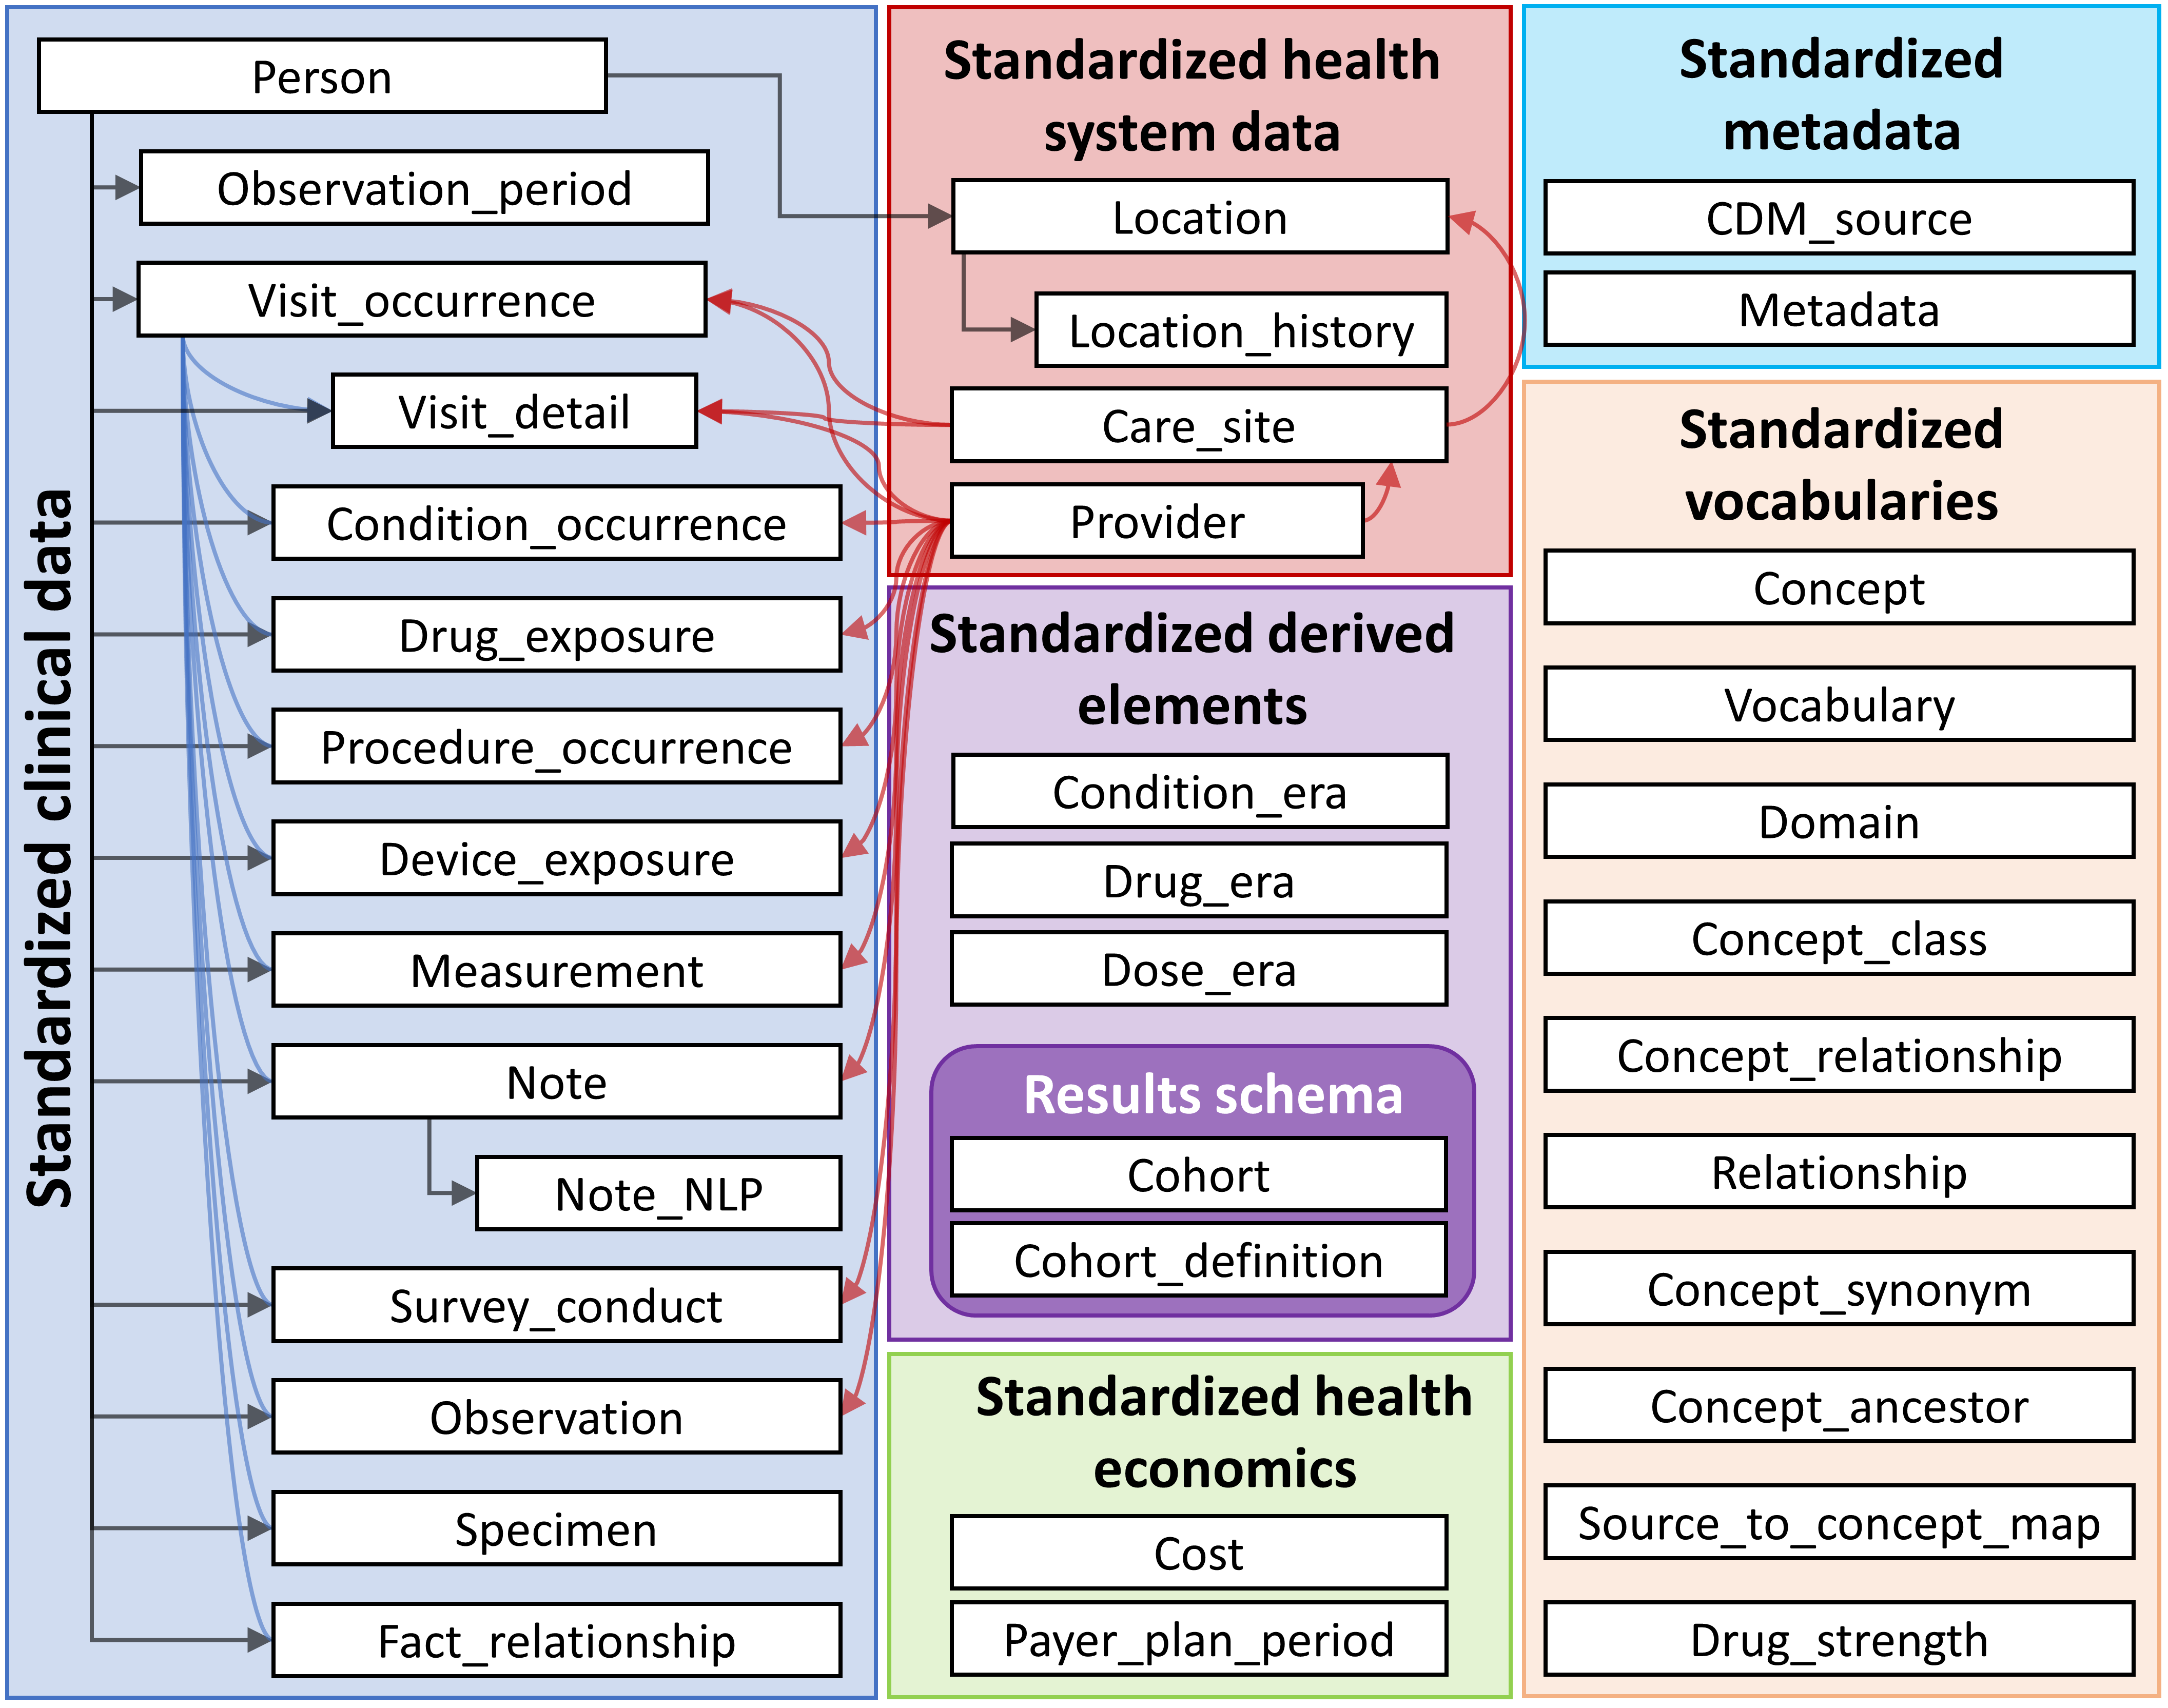
\includegraphics[width=1\linewidth]{images/CommonDataModel/cdmDiagram} \caption{Aperçu de toutes les tables dans le CDM version 6.0. Notez que toutes les relations entre les tables ne sont pas montrées.}\label{fig:cdmDiagram}
\end{figure}

\section{Principes de Conception}\label{principes-de-conception}

Le CDM est optimisé pour les objectifs typiques de la recherche observationnelle de \index{Common Data Model!principes de conception}

\begin{itemize}
\tightlist
\item
  Identifier les populations de patients avec certaines interventions de soins de santé (exposition aux médicaments, procédures, changements de politique de santé, etc.) et résultats (conditions, procédures, autres expositions aux médicaments, etc.),
\item
  Caractériser ces populations de patients pour divers paramètres comme les informations démographiques, l'histoire naturelle de la maladie, la prestation des soins de santé, l'utilisation et le coût, les morbidités, les traitements et la séquence de traitement, etc.,
\item
  Prédire l'apparition de ces résultats chez les patients individuels - voir Chapitre \ref{PatientLevelPrediction},
\item
  Estimer l'effet de ces interventions sur une population - voir Chapitre \ref{PopulationLevelEstimation},
\end{itemize}

Pour atteindre cet objectif, le développement du CDM suit les éléments de conception suivants :

\begin{itemize}
\tightlist
\item
  \textbf{Adéquation à l'objectif} : Le CDM vise à fournir des données organisées de manière optimale pour l'analyse, plutôt que pour répondre aux besoins opérationnels des fournisseurs de soins de santé ou des payeurs. \index{Common Data Model!adéquation à l'objectif}
\item
  \textbf{Protection des données} : Toutes les données pouvant compromettre l'identité et la protection des patients, telles que les noms, les dates d'anniversaire précises, etc., sont limitées. Des exceptions sont possibles lorsque la recherche nécessite expressément des informations plus détaillées, telles que des dates de naissance précises pour l'étude des nourrissons.\index{Common Data Model!protection des données}
\item
  \textbf{Conception des domaines} : Les domaines sont modélisés dans un modèle de données relationnelles centré sur la personne, où pour chaque enregistrement l'identité de la personne et une date sont capturées comme minimum. Ici, un modèle de données relationnelles est un modèle où les données sont représentées comme une collection de tables liées par des clés primaires et étrangères.
\item
  \textbf{Raison d'être des domaines} : Les domaines sont identifiés et définis séparément dans un modèle entité-relation s'ils ont un cas d'utilisation analytique (les conditions, par exemple) et le domaine a des attributs spécifiques qui ne sont pas autrement applicables. Toutes les autres données peuvent être conservées comme une observation dans la table des observations dans une structure entité-attribut-valeur. \index{Common Data Model!domaines}
\item
  \textbf{Vocabulaires standardisés} : Pour normaliser le contenu de ces enregistrements, le CDM repose sur les Vocabulaires Standardisés contenant tous les concepts de soins de santé nécessaires et appropriés correspondants.
\item
  \textbf{Réutilisation des vocabulaires existants} : Si possible, ces concepts sont tirés d'organisations ou d'initiatives de normalisation nationale ou sectorielle de définition de vocabulaire, telles que la Bibliothèque Nationale de Médecine, le Département des Anciens Combattants, le Centre de Contrôle et de Prévention des Maladies, etc.
\item
  \textbf{Maintien des codes sources} : Même si tous les codes sont mappés aux Vocabulaires Standardisés, le modèle stocke également le code source original pour garantir qu'aucune information n'est perdue. \index{Common Data Model!Codes Sources} \index{Common Data Model!prévention de la perte de données}
\item
  \textbf{Neutralité technologique} : Le CDM ne nécessite pas de technologie spécifique. Il peut être réalisé dans n'importe quelle base de données relationnelle, telle qu'Oracle, SQL Server, etc., ou sous forme de jeux de données analytiques SAS.\index{Common Data Model!neutralité technologique}
\item
  \textbf{Scalabilité} : Le CDM est optimisé pour le traitement des données et l'analyse computationnelle afin de s'adapter aux sources de données de tailles variées, y compris les bases de données avec jusqu'à des centaines de millions de personnes et des milliards d'observations cliniques. \index{Common Data Model!scalabilité}
\item
  \textbf{Compatibilité ascendante} : Tous les changements par rapport aux versions précédentes du CDM sont clairement délimités dans le dépôt github \href{https://github.com/OHDSI/CommonDataModel}{(https://github.com/OHDSI/CommonDataModel)}. Les versions plus anciennes du CDM peuvent être facilement créées à partir de la version actuelle, et aucune information n'est perdue qui était présente précédemment. \index{Common Data Model!compatibilité ascendante}
  \#\# Conventions du Modèle de Données
\end{itemize}

De nombreuses conventions implicites et explicites ont été adoptées dans le CDM. Les développeurs de méthodes qui fonctionnent avec le CDM doivent comprendre ces conventions. \index{Common Data Model!conventions}

\subsection{Conventions Générales du Modèle}\label{model-Conv}

Le CDM est considéré comme un modèle ``centré sur la personne'', ce qui signifie que toutes les tables d'événements cliniques sont liées à la table PERSON. Associé à la date ou à la date de début, cela permet une vue longitudinale de tous les événements pertinents pour la santé par personne. Les exceptions à cette règle sont les tables de données du système de santé standardisées, qui sont directement liées aux événements des différents domaines.

\subsection{Conventions Générales des Schémas}\label{conventions-guxe9nuxe9rales-des-schuxe9mas}

Les schémas, ou utilisateurs de bases de données dans certains systèmes, permettent une séparation entre les tables en lecture seule et les tables en lecture-écriture. Les tables d'événements cliniques et de vocabulaire sont dans le schéma ``CDM'' et sont considérées comme en lecture seule pour l'utilisateur final ou l'outil analytique. Les tables qui doivent être manipulées par des outils en ligne ou des utilisateurs finaux sont stockées dans le schéma ``Results''. Les deux tables du schéma ``Results'' sont COHORT et COHORT\_DEFINITION. Ces tables sont destinées à décrire des groupes d'intérêt que l'utilisateur pourrait définir, comme détaillé dans le chapitre \ref{Cohorts}. Ces tables peuvent être écrites, ce qui signifie qu'une cohorte peut être stockée dans la table COHORT au moment de l'exécution. Comme il n'y a qu'un seul schéma en lecture-écriture pour tous les utilisateurs, il appartient à l'implémentation du CDM d'organiser et de contrôler l'accès multiple des utilisateurs.

\subsection{Conventions Générales des Tables de Données}\label{conventions-guxe9nuxe9rales-des-tables-de-donnuxe9es}

Le CDM est indépendant de la plateforme. Les types de données sont définis de manière générique en utilisant les types de données ANSI SQL (VARCHAR, INTEGER, FLOAT, DATE, DATETIME, CLOB). La précision n'est fournie que pour VARCHAR. Elle reflète la longueur minimale requise de la chaîne, mais peut être étendue dans une instanciation concrète du CDM. Le CDM ne prescrit pas le format de date et datetime. Les requêtes standard contre le CDM peuvent varier pour les instances locales et les configurations de date/datetime.

\emph{Remarque}: Bien que le modèle de données lui-même soit indépendant de la plateforme, de nombreux outils développés pour fonctionner avec celui-ci nécessitent certaines spécifications. Pour plus d'informations à ce sujet, veuillez consulter le chapitre \ref{OhdsiAnalyticsTools}.

\subsection{Conventions Générales des Domaines}\label{domains}

Les événements de nature différente sont organisés en domaines. Ces événements sont stockés dans des tables et des champs spécifiques aux domaines et représentés par des concepts standard spécifiques aux domaines tels que définis dans les vocabulaires standardisés (voir section \ref{conceptDomains}). Chaque concept standard a une affectation de domaine unique, qui définit dans quelle table ils sont enregistrés. Même si l'affectation correcte des domaines fait l'objet de débats dans la communauté, cette règle stricte de correspondance domaine-table-champ garantit qu'il y a toujours un emplacement sans ambiguïté pour tout code ou concept. Par exemple, les signes, symptômes et concepts de diagnostic appartiennent au domaine Condition et sont enregistrés dans le CONDITION\_CONCEPT\_ID de la table CONDITION\_OCCURRENCE. Les soi-disant médicaments de procédure sont généralement enregistrés sous forme de codes de procédure dans une table de procédures dans les données source. Dans un CDM, ces enregistrements se trouvent dans la table DRUG\_EXPOSURE car les concepts standard mappés ont l'affectation de domaine Drug. Il y a un total de 30 domaines, comme le montre le tableau \ref{tab:domains}.

\begin{longtable}[]{@{}llll@{}}
\caption{\label{tab:domains} Nombre de concepts standard appartenant à chaque domaine.}\tabularnewline
\toprule\noalign{}
Nombre de Concepts & ID du Domaine & Nombre de Concepts & ID du Domaine \\
\midrule\noalign{}
\endfirsthead
\toprule\noalign{}
Nombre de Concepts & ID du Domaine & Nombre de Concepts & ID du Domaine \\
\midrule\noalign{}
\endhead
\bottomrule\noalign{}
\endlastfoot
1731378 & Drug & 183 & Route \\
477597 & Device & 180 & Currency \\
257000 & Procedure & 158 & Payer \\
163807 & Condition & 123 & Visit \\
145898 & Observation & 51 & Cost \\
89645 & Measurement & 50 & Race \\
33759 & Spec Anatomic Site & 13 & Plan Stop Reason \\
17302 & Meas Value & 11 & Plan \\
1799 & Specimen & 6 & Episode \\
1215 & Provider Specialty & 6 & Sponsor \\
1046 & Unit & 5 & Meas Value Operator \\
944 & Metadata & 3 & Spec Disease Status \\
538 & Revenue Code & 2 & Gender \\
336 & Type Concept & 2 & Ethnicity \\
194 & Relationship & 1 & Observation Type \\
\end{longtable}

\subsection{Représentation du Contenu par des Concepts}\label{repruxe9sentation-du-contenu-par-des-concepts}

Dans les tables de données du CDM, le contenu de chaque enregistrement est entièrement normalisé et représenté par des concepts. Les concepts sont stockés dans les tables d'événements avec leurs valeurs CONCEPT\_ID, lesquelles sont des clés étrangères vers la table CONCEPT, qui sert de table de référence générale. Toutes les instances de CDM utilisent la même table CONCEPT comme référence des concepts, ce qui, avec le Common Data Model, est un mécanisme clé d'interopérabilité et la fondation du réseau de recherche OHDSI. Si un concept standard n'existe pas ou ne peut pas être identifié, la valeur de CONCEPT\_ID est définie à 0, représentant un concept inexistant, une valeur inconnue ou non mappable.

Les enregistrements dans la table CONCEPT contiennent des informations détaillées sur chaque concept (nom, domaine, classe, etc.). Les concepts, les relations entre concepts, les ancêtres de concepts et d'autres informations relatives aux concepts sont contenus dans les tables des vocabulaires standardisés (voir chapitre \ref{StandardizedVocabularies}).

\subsection{Conventions Générales de Nomination des Champs}\label{conventions-guxe9nuxe9rales-de-nomination-des-champs}

Les noms de variables dans toutes les tables suivent une convention :

\begin{longtable}[]{@{}
  >{\raggedright\arraybackslash}p{(\columnwidth - 2\tabcolsep) * \real{0.4211}}
  >{\raggedright\arraybackslash}p{(\columnwidth - 2\tabcolsep) * \real{0.5789}}@{}}
\caption{\label{tab:fieldConventions} Conventions de dénomination des champs.}\tabularnewline
\toprule\noalign{}
\begin{minipage}[b]{\linewidth}\raggedright
Notation
\end{minipage} & \begin{minipage}[b]{\linewidth}\raggedright
Description
\end{minipage} \\
\midrule\noalign{}
\endfirsthead
\toprule\noalign{}
\begin{minipage}[b]{\linewidth}\raggedright
Notation
\end{minipage} & \begin{minipage}[b]{\linewidth}\raggedright
Description
\end{minipage} \\
\midrule\noalign{}
\endhead
\bottomrule\noalign{}
\endlastfoot
{[}Event{]}\_ID & Identifiant unique pour chaque enregistrement, qui sert de clé étrangère pour établir des relations entre les tables d'événements. Par exemple, PERSON\_ID identifie chaque individu de manière unique. VISIT\_OCCURRENCE\_ID identifie de manière unique une visite. \\
{[}Event{]}\_CONCEPT\_ID & Clé étrangère vers un enregistrement de concept standard dans la table de référence CONCEPT. C'est la principale représentation de l'événement, servant de base principale pour toutes les analyses standardisées. Par exemple, CONDITION\_CONCEPT\_ID = \href{http://athena.ohdsi.org/search-terms/terms/31967}{31967} contient la valeur de référence pour le concept SNOMED de ``Nausée''. \\
{[}Event{]}\_SOURCE\_CONCEPT\_ID & Clé étrangère vers un enregistrement de la table de référence CONCEPT. Ce concept est l'équivalent de la valeur source (ci-dessous), et il peut s'agir d'un concept standard, auquel cas il serait identique à {[}Event{]}\_CONCEPT\_ID, ou un autre concept non standard. Par exemple, CONDITION\_SOURCE\_CONCEPT\_ID = \href{http://athena.ohdsi.org/search-terms/terms/45431665}{45431665} dénote le concept de ``Nausée'' dans la terminologie Read, et l'analogue CONDITION\_CONCEPT\_ID est le concept standard SNOMED-CT \href{http://athena.ohdsi.org/search-terms/terms/31967}{31967}. L'utilisation des concepts de source pour les applications analytiques standard est déconseillée car seuls les concepts standard représentent le contenu sémantique d'un événement de manière non équivoque et, par conséquent, les concepts de source ne sont pas interopérables. \\
{[}Event{]}\_TYPE\_CONCEPT\_ID & Clé étrangère vers un enregistrement de la table de référence CONCEPT, représentant l'origine de l'information source, standardisée dans les vocabulaires standardisés. Notez que malgré le nom du champ, ce n'est pas un type d'événement ou un type de concept, mais cela déclare le mécanisme de capture qui a créé cet enregistrement. Par exemple, DRUG\_TYPE\_CONCEPT\_ID discrimine si un enregistrement de médicament a été dérivé d'un événement de délivrance en pharmacie (``Délivrance en pharmacie'') ou d'une application de prescription électronique (``Prescription rédigée''). \\
{[}Event{]}\_SOURCE\_VALUE & Code littéral ou chaîne de texte libre reflétant comment cet événement était représenté dans les données sources. Son utilisation est déconseillée pour les applications analytiques standard, car ces valeurs sources ne sont pas harmonisées entre les différentes sources de données. Par exemple, CONDITION\_SOURCE\_VALUE pourrait contenir un enregistrement de ``78702'', correspondant au code ICD-9 787.02 écrit dans une notation omettant le point. \\
\end{longtable}

\subsection{Différence Entre Concepts et Valeurs Sources}\label{concepts-Sources}

De nombreuses tables contiennent des informations équivalentes à plusieurs endroits : comme une valeur source, un concept de source et comme un concept standard.

\begin{itemize}
\tightlist
\item
  \textbf{Valeurs sources} sont la représentation originale d'un enregistrement d'événement dans les données sources. Elles peuvent être des codes provenant de systèmes de codage largement utilisés et souvent de domaine public, tels que ICD9CM, NDC ou Read, des systèmes de codage propriétaires comme CPT4, GPI ou MedDRA, ou des vocabulaires contrôlés utilisés uniquement dans les données sources, tels que F pour féminin et M pour masculin. Elles peuvent également être de courtes phrases de texte libre qui ne sont pas standardisées et contrôlées. Les valeurs sources sont stockées dans les champs {[}Event{]}\_SOURCE\_VALUE des tables de données.
\item
  \textbf{Concepts} sont des entités spécifiques au CDM qui normalisent la signification d'un fait clinique. La plupart des concepts sont basés sur des systèmes de codage publics ou propriétaires existants dans le domaine de la santé, tandis que d'autres ont été créés de novo (le CONCEPT\_CODE commence par ``OMOP''). Les concepts ont des identifiants uniques dans tous les domaines.
\item
  \textbf{Concepts de source} sont les concepts qui représentent le code utilisé dans la source. Les concepts de source ne sont utilisés que pour les systèmes de codage publics ou propriétaires existants, pas pour les concepts générés par OMOP. Les concepts de source sont stockés dans le champ {[}Event{]}\_SOURCE\_CONCEPT\_ID des tables de données.
\item
  \textbf{Concepts standards} sont ceux qui sont utilisés pour définir de manière unique la signification d'une entité clinique dans toutes les bases de données, indépendamment du système de codage utilisé dans les sources. Les concepts standards sont généralement tirés de sources de vocabulaire publiques ou propriétaires existantes. Les concepts non standard qui ont une signification équivalente à un concept standard ont une mappage vers le concept standard dans les vocabulaires standardisés. Les concepts standards sont référencés dans le champ {[}Event{]}\_CONCEPT\_ID des tables de données.
\end{itemize}

Les valeurs sources ne sont fournies que pour des raisons de commodité et de garantie de qualité (QA). Elles peuvent contenir des informations qui ne sont significatives que dans le contexte d'une source de données spécifique. L'utilisation des valeurs sources et des concepts de source est facultative, bien que \textbf{fortement recommandée} si les données sources utilisent des systèmes de codage. Cependant, les concepts standards \textbf{sont obligatoires}. Cette utilisation obligatoire de concepts standards est ce qui permet à toutes les instances de CDM de parler le même langage. Par exemple, la condition ``Tuberculose pulmonaire'' (TB, Figure \ref{fig:pulmTubICD9}) montre que le code ICD9CM pour la TB est 011.

\begin{figure}

{\centering 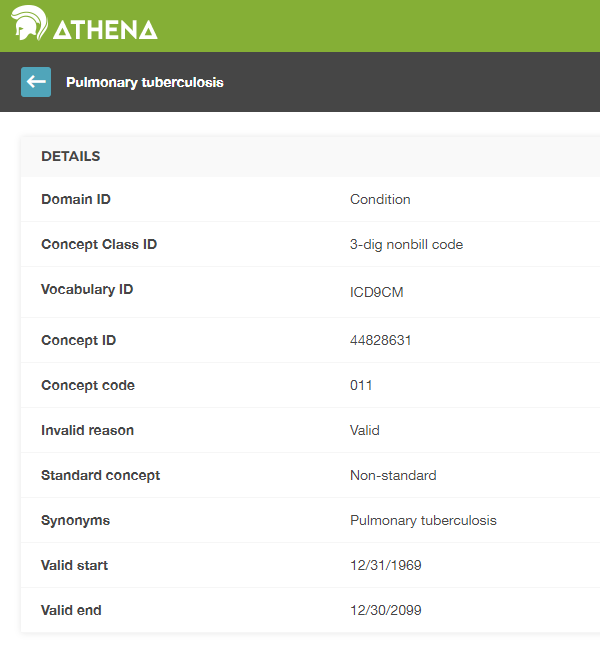
\includegraphics[width=0.75\linewidth]{images/CommonDataModel/pulmTubICD9} 

}

\caption{ICD9CM code for Pulmonary Tuberculosis}\label{fig:pulmTubICD9}
\end{figure}

Sans contexte, le code 011 pourrait être interprété comme ``Hospital Inpatient (Including Medicare Part A)'' du vocabulaire UB04, ou comme ``Nervous System Neoplasms without Complications, Comorbidities'' du vocabulaire DRG. C'est ici que les identifiants de concepts, qu'ils soient de source ou standards, sont précieux. La valeur CONCEPT\_ID qui représente le code 011 ICD9CM est \href{http://athena.ohdsi.org/search-terms/terms/44828631}{44828631}. Cela différencie l'ICD9CM du UBO4 et du DRG. Le concept de source ICD9CM TB se mappe sur le concept standard \href{http://athena.ohdsi.org/search-terms/terms/253954}{253954} du vocabulaire SNOMED à travers la relation ``Non-standard to Standard map (OMOP)'' comme montré dans la figure \ref{fig:pulmTubMap}. Cette même relation de mappage existe pour les codes Read, ICD10, CIEL et MeSH, entre autres, de sorte que toute recherche qui se réfère au concept standard SNOMED est sûre d'inclure tous les codes sources supportés.

\begin{figure}
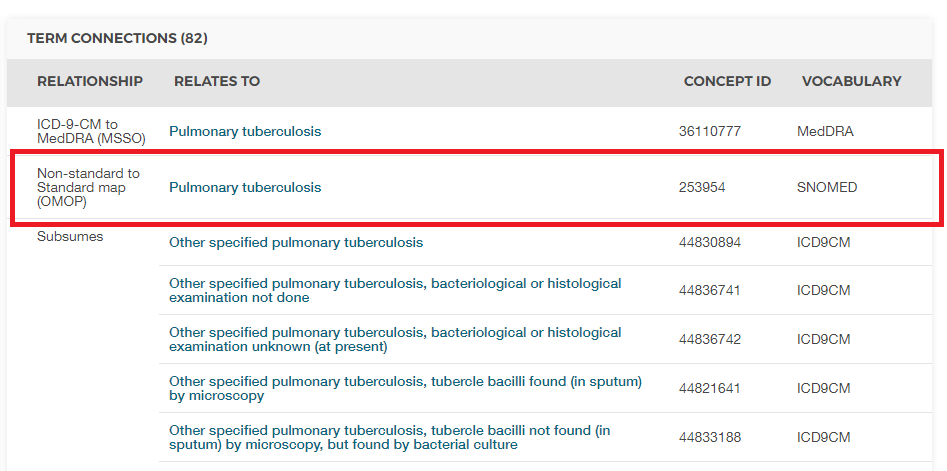
\includegraphics[width=1\linewidth]{images/CommonDataModel/pulmTubMap} \caption{SNOMED code for Pulmonary Tuberculosis}\label{fig:pulmTubMap}
\end{figure}

Un exemple de la manière dont la relation entre concept standard et concept de source est représentée est montré dans le tableau \ref{tab:conditionOccurrence}.
\#\# Tables standardisées CDM

\index{Common Data Model!tableaux standardisés}

La CDM contient 16 tableaux d'événements cliniques, 10 tableaux de vocabulaire, 2 tableaux de métadonnées, 4 tableaux de données relatives au système de santé, 2 tableaux de données économiques de santé, 3 éléments dérivés standardisés et 2 tableaux de schéma de résultats. Ces tableaux sont entièrement spécifiés dans le Wiki CDM.\footnote{\url{https://github.com/OHDSI/CommonDataModel/wiki}}

Pour illustrer comment ces tableaux sont utilisés en pratique, les données d'une personne seront utilisées comme fil conducteur tout au long du reste du chapitre.

\subsection{Exemple en cours : Endométriose}\label{exemple-en-cours-endomuxe9triose}

L'endométriose est une condition douloureuse dans laquelle des cellules normalement présentes dans la paroi de l'utérus d'une femme se trouvent ailleurs dans le corps. Les cas sévères peuvent entraîner l'infertilité, ainsi que des problèmes intestinaux et urinaires. Les sections suivantes détailleront l'expérience d'une patiente avec cette maladie et comment elle pourrait être représentée dans le Modèle de Données Commun.

\begin{center}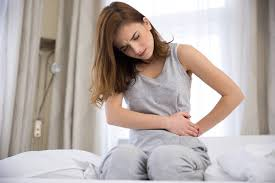
\includegraphics[width=0.5\linewidth]{images/CommonDataModel/Lauren} \end{center}

\begin{quote}
Chaque étape de ce douloureux parcours, j'ai dû convaincre tout le monde de la douleur que je ressentais.
\end{quote}

Lauren souffrait des symptômes de l'endométriose depuis de nombreuses années ; cependant, ce n'est qu'après la rupture d'un kyste dans son ovaire qu'elle a été diagnostiquée. Vous pouvez en savoir plus sur Lauren à \url{https://endometriosis-uk.org/laurens-story}.

\subsection{Tableau PERSON}\label{person}

\subsubsection*{Que savons-nous de Lauren?}\label{que-savons-nous-de-lauren}
\addcontentsline{toc}{subsubsection}{Que savons-nous de Lauren?}

\begin{itemize}
\tightlist
\item
  Elle est une femme de 36 ans
\item
  Son anniversaire est le 12 mars 1982
\item
  Elle est blanche
\item
  Elle est anglaise
\end{itemize}

Avec cela en tête, son tableau PERSON pourrait ressembler à ceci :

Tableau: \label{tab:person} Le tableau PERSON.

\begin{longtable}[]{@{}
  >{\raggedright\arraybackslash}p{(\columnwidth - 4\tabcolsep) * \real{0.3014}}
  >{\raggedright\arraybackslash}p{(\columnwidth - 4\tabcolsep) * \real{0.1644}}
  >{\raggedright\arraybackslash}p{(\columnwidth - 4\tabcolsep) * \real{0.5342}}@{}}
\toprule\noalign{}
\begin{minipage}[b]{\linewidth}\raggedright
Nom de colonne
\end{minipage} & \begin{minipage}[b]{\linewidth}\raggedright
Valeur
\end{minipage} & \begin{minipage}[b]{\linewidth}\raggedright
Explication
\end{minipage} \\
\midrule\noalign{}
\endhead
\bottomrule\noalign{}
\endlastfoot
PERSON\_ID & 1 & Le PERSON\_ID doit être un entier, soit directement issu de la source soit généré dans le cadre du processus de création. \\
GENDER\_CONCEPT\_ID & 8532 & L'ID de concept se référant au genre féminin est \href{http://athena.ohdsi.org/search-terms/terms/8532}{8532}. \\
YEAR\_OF\_BIRTH & 1982 & \\
MONTH\_OF\_BIRTH & 3 & \\
DAY\_OF\_BIRTH & 12 & \\
BIRTH\_DATETIME & 1982-03-12 00:00:00 & Lorsque l'heure n'est pas connue, minuit est utilisé. \\
DEATH\_DATETIME & & \\
RACE\_CONCEPT\_ID & 8527 & L'ID de concept se référant à la race blanche est \href{http://athena.ohdsi.org/search-terms/terms/8527}{8527}. L'ethnicité anglaise est \href{http://athena.ohdsi.org/search-terms/terms/4093769}{4093769}. L'un ou l'autre est correct, ce dernier correspondant au premier. Notez que les ethnicités sont stockées ici en tant que races, et non dans le ETHNICITY\_CONCEPT\_ID \\
ETHNICITY\_CONCEPT\_ ID & 38003564 & C'est une notation typique des États-Unis pour distinguer les Hispaniques des autres. Les ethnicités, dans ce cas anglaise, sont stockées dans le RACE\_CONCEPT\_ID. En dehors des États-Unis, cela n'est pas utilisé. \href{http://athena.ohdsi.org/search-terms/terms/38003564}{38003564} se réfère à ``Non hispanique''. \\
LOCATION\_ID & & Son adresse est inconnue. \\
PROVIDER\_ID & & Son médecin traitant est inconnu. \\
CARE\_SITE & & Son site de soins principal est inconnu. \\
PERSON\_SOURCE\_ VALUE & 1 & Il s'agirait généralement de son identifiant dans les données sources, bien que souvent il soit le même que le PERSON\_ID. \\
GENDER\_SOURCE\_ VALUE & F & La valeur du genre telle qu'elle apparaît dans la source est stockée ici. \\
GENDER\_SOURCE\_ CONCEPT\_ID & 0 & Si la valeur du genre dans la source était codée en utilisant un schéma de codage pris en charge par OHDSI, ce concept irait ici. Par exemple, si son genre était ``sex-F'' dans la source et qu'il était indiqué être dans le vocabulaire PCORNet, le concept \href{http://athena.ohdsi.org/search-terms/terms/44814665}{44814665} irait dans ce champ. \\
RACE\_SOURCE\_ VALUE & white & La valeur de la race telle qu'elle apparaît dans la source est stockée ici. \\
RACE\_SOURCE\_ CONCEPT\_ID & 0 & Même principe que GENDER\_SOURCE\_CONCEPT\_ID. \\
ETHNICITY\_SOURCE\_ VALUE & english & La valeur de l'ethnicité telle qu'elle apparaît dans la source est stockée ici. \\
ETHNICITY\_SOURCE\_ CONCEPT\_ID & 0 & Même principe que GENDER\_SOURCE\_CONCEPT\_ID. \\
\end{longtable}

\subsection{Tableau OBSERVATION\_PERIOD}\label{observationPeriod}

Le tableau OBSERVATION\_PERIOD est conçu pour définir la période pendant laquelle au moins les données démographiques, les conditions, les procédures et les médicaments d'un patient sont enregistrées dans le système source avec une sensibilité et une spécificité raisonnables. Pour les données d'assurance, cela correspond généralement à la période d'inscription du patient. C'est plus compliqué dans les dossiers de santé électroniques (EHR), car la plupart des systèmes de santé ne déterminent pas quel établissement ou fournisseur de soins de santé est visité. En tant que meilleure solution alternative, le premier enregistrement du système est souvent considéré comme la date de début de la période d'observation et le dernier enregistrement est considéré comme la date de fin.

\subsubsection*{Comment est définie la période d'observation de Lauren?}\label{comment-est-duxe9finie-la-puxe9riode-dobservation-de-lauren}
\addcontentsline{toc}{subsubsection}{Comment est définie la période d'observation de Lauren?}

Disons que les informations de Lauren, comme montré dans le Tableau \ref{tab:encounters}, sont enregistrées comme dans un système EHR. Ses rencontres à partir desquelles la période d'observation a été dérivée sont :

Tableau: \label{tab:encounters} Rencontres de soins de santé de Lauren.

\begin{longtable}[]{@{}llll@{}}
\toprule\noalign{}
ID de rencontre & Date de début & Date de fin & Type \\
\midrule\noalign{}
\endhead
\bottomrule\noalign{}
\endlastfoot
70 & 2010-01-06 & 2010-01-06 & ambulatoire \\
80 & 2011-01-06 & 2011-01-06 & ambulatoire \\
90 & 2012-01-06 & 2012-01-06 & ambulatoire \\
100 & 2013-01-07 & 2013-01-07 & ambulatoire \\
101 & 2013-01-14 & 2013-01-14 & ambulatoire \\
102 & 2013-01-17 & 2013-01-24 & hospitalisation \\
\end{longtable}

Sur la base des enregistrements de rencontre, son tableau OBSERVATION\_PERIOD pourrait ressembler à ceci :

Tableau: \label{tab:observationPeriod} Le tableau OBSERVATION\_PERIOD.

\begin{longtable}[]{@{}
  >{\raggedright\arraybackslash}p{(\columnwidth - 4\tabcolsep) * \real{0.3151}}
  >{\raggedright\arraybackslash}p{(\columnwidth - 4\tabcolsep) * \real{0.1507}}
  >{\raggedright\arraybackslash}p{(\columnwidth - 4\tabcolsep) * \real{0.5342}}@{}}
\toprule\noalign{}
\begin{minipage}[b]{\linewidth}\raggedright
Nom de colonne
\end{minipage} & \begin{minipage}[b]{\linewidth}\raggedright
Valeur
\end{minipage} & \begin{minipage}[b]{\linewidth}\raggedright
Explication
\end{minipage} \\
\midrule\noalign{}
\endhead
\bottomrule\noalign{}
\endlastfoot
OBSERVATION\_ PERIOD\_ID & 1 & Il s'agit généralement d'une valeur générée automatiquement, créant un identifiant unique pour chaque enregistrement dans le tableau. \\
PERSON\_ID & 1 & Ceci est une clé étrangère vers l'enregistrement de Laura dans le tableau PERSON et lie PERSON au tableau OBSERVATION\_PERIOD. \\
OBSERVATION\_PERIOD\_ START\_DATE & 2010-01-06 & Il s'agit de la date de début de sa première rencontre enregistrée. \\
OBSERVATION\_PERIOD\_ END\_DATE & 2013-01-24 & Il s'agit de la date de fin de sa dernière rencontre enregistrée. \\
PERIOD\_TYPE\_ CONCEPT\_ID & 44814725 & La meilleure option dans le Vocabulaire avec la catégorie de concept ``Type de période d'observation'' est \href{http://athena.ohdsi.org/search-terms/terms/44814724}{44814724}, qui représente ``Période couvrant les rencontres de soins de santé''. \\
\end{longtable}

\subsection{VISIT\_OCCURRENCE}\label{visitOccurrence}

Le tableau VISIT\_OCCURRENCE contient des informations sur les rencontres des patients avec le système de santé. Dans la terminologie OHDSI, celles-ci sont appelées visites et sont considérées comme des événements distincts. Il existe 12 catégories principales de visites avec une hiérarchie étendue, représentant les nombreuses différentes circonstances dans lesquelles les soins de santé peuvent être dispensés. Les visites les plus couramment enregistrées sont les hospitalisations, les consultations externes, les urgences et les visites dans des institutions non médicales.

\subsubsection*{Comment les rencontres de Lauren sont-elles représentées en tant que visites?}\label{comment-les-rencontres-de-lauren-sont-elles-repruxe9sentuxe9es-en-tant-que-visites}
\addcontentsline{toc}{subsubsection}{Comment les rencontres de Lauren sont-elles représentées en tant que visites?}

À titre d'exemple, représentons la rencontre hospitalière dans le Tableau \ref{tab:encounters} dans le tableau VISIT\_OCCURRENCE.

Tableau: \label{tab:visitOccurrence} Le tableau VISIT\_OCCURRENCE.

\begin{longtable}[]{@{}
  >{\raggedright\arraybackslash}p{(\columnwidth - 4\tabcolsep) * \real{0.3014}}
  >{\raggedright\arraybackslash}p{(\columnwidth - 4\tabcolsep) * \real{0.1644}}
  >{\raggedright\arraybackslash}p{(\columnwidth - 4\tabcolsep) * \real{0.5342}}@{}}
\toprule\noalign{}
\begin{minipage}[b]{\linewidth}\raggedright
Nom de colonne
\end{minipage} & \begin{minipage}[b]{\linewidth}\raggedright
Valeur
\end{minipage} & \begin{minipage}[b]{\linewidth}\raggedright
Explication
\end{minipage} \\
\midrule\noalign{}
\endhead
\bottomrule\noalign{}
\endlastfoot
VISIT\_OCCURRENCE\_ ID & 514 & Il s'agit généralement d'une valeur générée automatiquement créant un identifiant unique pour chaque enregistrement. \\
PERSON\_ID & 1 & Ceci est une clé étrangère vers l'enregistrement de Laura dans le tableau PERSON et lie PERSON à VISIT\_OCCURRENCE. \\
VISIT\_CONCEPT\_ID & 9201 & Une clé étrangère se référant à une visite hospitalière est \href{http://athena.ohdsi.org/search-terms/terms/9201}{9201}. \\
VISIT\_START\_DATE & 2013-01-17 & La date de début de la visite. \\
VISIT\_START\_ DATETIME & 2013-01-17 00:00:00 & La date et l'heure de la visite. L'heure est inconnue, donc minuit est utilisé. \\
VISIT\_END\_DATE & 2013-01-24 & La date de fin de la visite. Si c'est une visite d'une seule journée, la date de fin doit correspondre à la date de début. \\
VISIT\_END\_DATETIME & 2013-01-24 00:00:00 & La date et l'heure de fin de la visite. L'heure est inconnue, donc minuit est utilisé. \\
VISIT\_TYPE\_ CONCEPT\_ID & 32034 & Cela fournit des informations sur la provenance de l'enregistrement de la visite, i.e.~cela provient-il d'une réclamation d'assurance, d'une facturation hospitalière, d'un EHR, etc. Pour cet exemple, l'ID du concept \href{http://athena.ohdsi.org/search-terms/terms/32035}{32035} (``Visite dérivée d'un enregistrement de rencontre EHR'') est utilisé car les rencontres sont similaires aux dossiers de santé électroniques \\
PROVIDER\_ID* & NULL & Si l'enregistrement de la rencontre a un prestataire associé, l'ID de ce prestataire va dans ce champ. Cela devrait être le contenu du champ PROVIDER\_ID du tableau PROVIDER. \\
CARE\_SITE\_ID & NULL & Si l'enregistrement de la rencontre a un site de soins associé, l'ID de ce site de soins va dans ce champ. Cela devrait être le CARE\_SITE\_ID du tableau CARE\_SITE. \\
VISIT\_SOURCE\_ VALUE & inpatient & La valeur de la visite telle qu'elle apparaît dans la source va ici. Les données de Lauren ne l'ont pas. \\
VISIT\_SOURCE\_ CONCEPT\_ID & 0 & Si la valeur de la visite de la source est codée en utilisant un vocabulaire reconnu par OHDSI, la valeur CONCEPT\_ID représentant le code source se trouverait ici. Les données de Lauren ne l'ont pas. \\
ADMITTED\_FROM\_ CONCEPT\_ID & 0 & Si connu, cela contient un Concept représentant d'où le patient a été admis. Ce concept devrait avoir le domaine ``Visite''. Par exemple, si le patient a été admis à l'hôpital depuis son domicile, il contiendrait \href{http://athena.ohdsi.org/search-terms/terms/8536}{8536} (``Domicile''). \\
ADMITTED\_FROM\_ SOURCE\_CONCEPT\_ID & NULL & C'est la valeur de la source qui représente d'où le patient a été admis. En utilisant l'exemple ci-dessus, cela serait ``domicile''. \\
DISCHARGE\_TO\_ CONCEPT\_ID & 0 & Si connu, cela se réfère à un Concept représentant où le patient a été transféré à la sortie. Ce concept doit avoir le domaine ``Visite''. Par exemple, si un patient a été libéré dans un établissement de vie assistée, l'ID du concept serait \href{http://athena.ohdsi.org/search-terms/terms/8615}{8615} (``Établissement de vie assistée''). \\
DISCHARGE\_TO\_ SOURCE\_VALUE & 0 & C'est la valeur de la source qui représente où le patient a été transféré à la sortie. En utilisant l'exemple ci-dessus, cela serait ``Établissement de vie assistée''. \\
PRECEDING\_VISIT\_ OCCURRENCE\_ID & NULL & Cela désigne la visite immédiatement précédente. Contrairement à ADMITTED\_FROM\_CONCEPT\_ID, cela renvoie au véritable enregistrement de la visite plutôt qu'à un concept de visite. Notez qu'il n'y a pas d'enregistrement pour la visite suivante, les visites ne sont reliées que par ce champ. \\
\end{longtable}

\begin{itemize}
\tightlist
\item
  Un patient peut interagir avec plusieurs prestataires de soins de santé lors d'une même visite, comme c'est souvent le cas lors de séjours hospitaliers. Ces interactions peuvent être enregistrées dans le tableau VISIT\_DETAIL. Bien que non couvert en profondeur dans ce chapitre, vous pouvez en savoir plus sur le tableau VISIT\_DETAIL dans le \href{https://github.com/OHDSI/CommonDataModel/wiki/VISIT_DETAIL}{wiki CDM}.
\end{itemize}

\subsection{CONDITION\_OCCURRENCE}\label{conditionOccurrence}

Les enregistrements dans le tableau CONDITION\_OCCURRENCE sont des diagnostics, des signes ou des symptômes d'une condition soit observés par un prestataire, soit rapportés par le patient.

\subsubsection*{Quelles sont les conditions de Lauren?}\label{quelles-sont-les-conditions-de-lauren}
\addcontentsline{toc}{subsubsection}{Quelles sont les conditions de Lauren?}

En revisitant son témoignage, elle dit:

\begin{quote}
Il y a environ 3 ans, j'ai remarqué que mes règles, qui avaient toujours été douloureuses, devenaient de plus en plus douloureuses. J'ai commencé à ressentir une douleur vive juste à côté de mon côlon et à me sentir sensible et ballonnée autour de mon coccyx et de ma région pelvienne inférieure. Mes règles étaient devenues tellement douloureuses que je manquais 1 à 2 jours de travail par mois. Les analgésiques atténuaient parfois la douleur, mais souvent ils ne faisaient pas grand-chose.
\end{quote}

Le code SNOMED pour les crampes menstruelles douloureuses, autrement appelé dysménorrhée, est 266599000. Le Tableau \ref{tab:conditionOccurrence} montre comment cela serait représenté dans le tableau CONDITION\_OCCURRENCE:

Tableau: \label{tab:conditionOccurrence} Le tableau CONDITION\_OCCURRENCE.

\begin{longtable}[]{@{}
  >{\raggedright\arraybackslash}p{(\columnwidth - 4\tabcolsep) * \real{0.3014}}
  >{\raggedright\arraybackslash}p{(\columnwidth - 4\tabcolsep) * \real{0.1644}}
  >{\raggedright\arraybackslash}p{(\columnwidth - 4\tabcolsep) * \real{0.5342}}@{}}
\toprule\noalign{}
\begin{minipage}[b]{\linewidth}\raggedright
Nom de colonne
\end{minipage} & \begin{minipage}[b]{\linewidth}\raggedright
Valeur
\end{minipage} & \begin{minipage}[b]{\linewidth}\raggedright
Explication
\end{minipage} \\
\midrule\noalign{}
\endhead
\bottomrule\noalign{}
\endlastfoot
CONDITION\_ OCCURRENCE\_ID & 964 & Ceci est généralement une valeur générée automatiquement, créant un identifiant unique pour chaque enregistrement. \\
PERSON\_ID & 1 & Ceci est une clé étrangère vers l'enregistrement de Laura dans le tableau PERSON et lie PERSON à CONDITION\_OCCURRENCE. \\
CONDITION\_ CONCEPT\_ID & 194696 & Une clé étrangère se référant au code SNOMED 266599000 : \href{http://athena.ohdsi.org/search-terms/terms/194696}{194696}. \\
CONDITION\_START\_ DATE & 2010-01-06 & La date à laquelle l'instance de la condition est enregistrée. \\
CONDITION\_START\_ DATETIME & 2010-01-06 00:00:00 & La date et l'heure à laquelle l'instance de la condition est enregistrée. Minuit est utilisé car l'heure est inconnue. \\
CONDITION\_END\_ DATE & NULL & C'est la date à laquelle l'instance de la condition est considérée comme terminée, mais cela est rarement enregistré. \\
CONDITION\_END\_ DATETIME & NULL & Si connu, c'est la date et l'heure à laquelle l'instance de la condition est considérée comme terminée. \\
CONDITION\_TYPE\_ CONCEPT\_ID & 32020 & Cette colonne est destinée à fournir des informations sur la provenance de l'enregistrement, c'est-à-dire qu'il provient d'une réclamation d'assurance, d'un dossier de facturation hospitalière, d'un EHR, etc. Pour cet exemple, le concept \href{http://athena.ohdsi.org/search-terms/terms/32020}{32020} (``Diagnostic de rencontre EHR'') est utilisé car les rencontres sont similaires aux dossiers de santé électroniques. Les concepts dans ce champ devraient être dans le vocabulaire ``Condition Type''. \\
CONDITION\_STATUS\_ CONCEPT\_ID & 0 & Si connu, cela indique la circonstance. Par exemple, une condition pourrait être un diagnostic d'admission, auquel cas l'ID du concept \href{http://athena.ohdsi.org/search-terms/terms/4203942}{4203942} serait utilisé. \\
STOP\_REASON & NULL & Si connu, la raison pour laquelle la condition n'était plus présente, comme indiqué dans les données sources. \\
PROVIDER\_ID & NULL & Si l'enregistrement de la condition a un prestataire de diagnostic listé, l'ID de ce prestataire va dans ce champ. Cela devrait être le provider\_id du tableau PROVIDER représentant le prestataire lors de la rencontre. \\
VISIT\_OCCURRENCE\_ ID & 509 & La visite (clé étrangère vers le VISIT\_OCCURRENCE\_ID dans le tableau VISIT\_OCCURRENCE) au cours de laquelle la condition a été diagnostiquée. \\
CONDITION\_SOURCE\_ VALUE & 266599000 & C'est la valeur source originale représentant la condition. Dans le cas de Lauren, la dysménorrhée est stockée ici via le code SNOMED, tandis que le concept représentant le code allait vers CONDITION\_SOURCE\_CONCEPT\_ID et le concept standard mappé à partir de cela est stocké dans le champ CONDITION\_CONCEPT\_ID. \\
CONDITION\_SOURCE\_ CONCEPT\_ID & 194696 & Si la valeur de la condition de la source est codée en utilisant un vocabulaire reconnu par OHDSI, l'ID du concept représentant cette valeur irait ici. Dans l'exemple de la dysménorrhée, la valeur source est un code SNOMED, donc le concept représentant ce code est 194696. Dans ce cas, il a la même valeur que \\
\end{longtable}

\section{Informations supplémentaires}\label{informations-suppluxe9mentaires}

Ce chapitre couvre seulement une partie des tables disponibles dans le CDM comme exemples de la manière dont les données sont représentées. Vous êtes encouragés à visiter le site wiki\footnote{\url{https://github.com/OHDSI/CommonDataModel/wiki}} pour plus d'informations.

\section{Résumé}\label{ruxe9sumuxe9-2}

\begin{rmdsummary}
\begin{itemize}
\item
  Le CDM est conçu pour soutenir un large éventail d'activités de recherche observationnelle.
\item
  Le CDM est un modèle centré sur la personne.
\item
  Le CDM standardise non seulement la structure des données, mais grâce aux Vocabularies Standardisés, il standardise également la représentation du contenu.
\item
  Les codes sources sont maintenus dans le CDM pour une traçabilité complète.
\end{itemize}
\end{rmdsummary}

\section{Exercices}\label{exercices}

\subsubsection*{Prérequis}\label{pruxe9requis}
\addcontentsline{toc}{subsubsection}{Prérequis}

Pour ces premiers exercices, vous devrez revoir les tables du CDM discutées précédemment, et vous devrez rechercher des concepts dans le Vocabulary, ce qui peut être fait via ATHENA\footnote{\url{http://athena.ohdsi.org/}} ou ATLAS.\footnote{\url{http://atlas-demo.ohdsi.org}}

\begin{exercise}
\protect\hypertarget{exr:exerciseJohnPerson}{}\label{exr:exerciseJohnPerson}John est un homme afro-américain né le 4 août 1974. Définissez une entrée dans la table PERSON qui encode ces informations.
\end{exercise}

\begin{exercise}
\protect\hypertarget{exr:exerciseJohnOp}{}\label{exr:exerciseJohnOp}John s'est inscrit à son assurance actuelle le 1er janvier 2015. Les données de sa base de données d'assurance ont été extraites le 1er juillet 2019. Définissez une entrée dans la table OBSERVATION\_PERIOD qui encode ces informations.
\end{exercise}

\begin{exercise}
\protect\hypertarget{exr:exerciseJohnDrug}{}\label{exr:exerciseJohnDrug}On a prescrit à John une fourniture de 30 jours d'Ibuprofène 200 MG comprimés oraux (code NDC : 76168009520) le 1er mai 2019. Définissez une entrée dans la table DRUG\_EXPOSURE qui encode ces informations.
\end{exercise}

\subsubsection*{Prérequis}\label{pruxe9requis-1}
\addcontentsline{toc}{subsubsection}{Prérequis}

Pour ces trois derniers exercices, nous supposons que R, R-Studio et Java ont été installés comme décrit dans la Section \ref{installR}. Il est également nécessaire d'installer les packages \href{https://ohdsi.github.io/SqlRender/}{SqlRender}, \href{https://ohdsi.github.io/DatabaseConnector/}{DatabaseConnector} et \href{https://ohdsi.github.io/Eunomia/}{Eunomia}, qui peuvent être installés avec :

\begin{Shaded}
\begin{Highlighting}[]
\FunctionTok{install.packages}\NormalTok{(}\FunctionTok{c}\NormalTok{(}\StringTok{"SqlRender"}\NormalTok{, }\StringTok{"DatabaseConnector"}\NormalTok{, }\StringTok{"remotes"}\NormalTok{))}
\NormalTok{remotes}\SpecialCharTok{::}\FunctionTok{install\_github}\NormalTok{(}\StringTok{"ohdsi/Eunomia"}\NormalTok{, }\AttributeTok{ref =} \StringTok{"v1.0.0"}\NormalTok{)}
\end{Highlighting}
\end{Shaded}

Le package Eunomia fournit un jeu de données simulé dans le CDM qui fonctionnera à l'intérieur de votre session R locale. Les détails de connexion peuvent être obtenus avec :

\begin{Shaded}
\begin{Highlighting}[]
\NormalTok{connectionDetails }\OtherTok{\textless{}{-}}\NormalTok{ Eunomia}\SpecialCharTok{::}\FunctionTok{getEunomiaConnectionDetails}\NormalTok{()}
\end{Highlighting}
\end{Shaded}

Le schéma de la base de données CDM est ``main''. Voici un exemple de requête SQL pour récupérer une ligne de la table CONDITION\_OCCURRENCE :

\begin{Shaded}
\begin{Highlighting}[]
\FunctionTok{library}\NormalTok{(DatabaseConnector)}
\NormalTok{connection }\OtherTok{\textless{}{-}} \FunctionTok{connect}\NormalTok{(connectionDetails)}
\NormalTok{sql }\OtherTok{\textless{}{-}} \StringTok{"SELECT *}
\StringTok{FROM @cdm.condition\_occurrence}
\StringTok{LIMIT 1;"}
\NormalTok{result }\OtherTok{\textless{}{-}} \FunctionTok{renderTranslateQuerySql}\NormalTok{(connection, sql, }\AttributeTok{cdm =} \StringTok{"main"}\NormalTok{)}
\end{Highlighting}
\end{Shaded}

\begin{exercise}
\protect\hypertarget{exr:exerciseGiBleedRecords}{}\label{exr:exerciseGiBleedRecords}En utilisant SQL et R, récupérez tous les enregistrements de la condition ``Hémorragie gastro-intestinale'' (avec l'ID de concept \href{http://athena.ohdsi.org/search-terms/terms/192671}{192671}).
\end{exercise}

\begin{exercise}
\protect\hypertarget{exr:exercisePersonSource}{}\label{exr:exercisePersonSource}En utilisant SQL et R, récupérez tous les enregistrements de la condition ``Hémorragie gastro-intestinale'' en utilisant les codes sources. Cette base de données utilise la CIM-10, et le code CIM-10 pertinent est ``K92.2''.
\end{exercise}

\begin{exercise}
\protect\hypertarget{exr:exercisePerson61Records}{}\label{exr:exercisePerson61Records}En utilisant SQL et R, récupérez la période d'observation de la personne avec PERSON\_ID 61.
\end{exercise}

Les réponses suggérées peuvent être trouvées dans l'Appendice \ref{Cdmanswers}.

\chapter{Vocabulaire normalisé}\label{StandardizedVocabularies}

\index{vocabulaire normalisé}

\emph{Chefs de chapitre : Christian Reich \& Anna Ostropolets}

Les Vocabulaire normalisé OMOP, souvent désignés simplement sous le terme « le Vocabulaire », sont une partie fondamentale du réseau de recherche OHDSI, et une partie intégrante du Modèle de Données Commun (CDM). Ils permettent la standardisation des méthodes, des définitions et des résultats en définissant le contenu des données, ouvrant la voie à une véritable recherche et analyse en réseau à distance (derrière le pare-feu). Habituellement, trouver et interpréter le contenu des données de santé observationnelles, qu'il s'agisse de données structurées en utilisant des systèmes de codage ou consignées dans du texte libre, est complètement laissé aux chercheurs, qui doivent faire face à une myriade de façons différentes de décrire les événements cliniques. OHDSI nécessite une harmonisation non seulement à un format standardisé, mais aussi à un contenu standard rigoureux.

Dans ce chapitre, nous décrivons d'abord les principaux principes des Vocabulaire normalisé, leurs composantes, et les règles, conventions et quelques situations typiques, qui sont toutes nécessaires pour comprendre et utiliser cette ressource fondamentale. Nous pointons également les domaines où le support de la communauté est nécessaire pour l'améliorer continuellement.

\section{Pourquoi les vocabulaires, et pourquoi les normaliser}\label{pourquoi-les-vocabulaires-et-pourquoi-les-normaliser}

Les vocabulaires médicaux remontent aux Bills of Mortality dans le Londres médiéval pour gérer les épidémies de peste et d'autres maladies (voir Figure \ref{fig:bill}). \index{Bill of Mortality}

\begin{figure}

{\centering 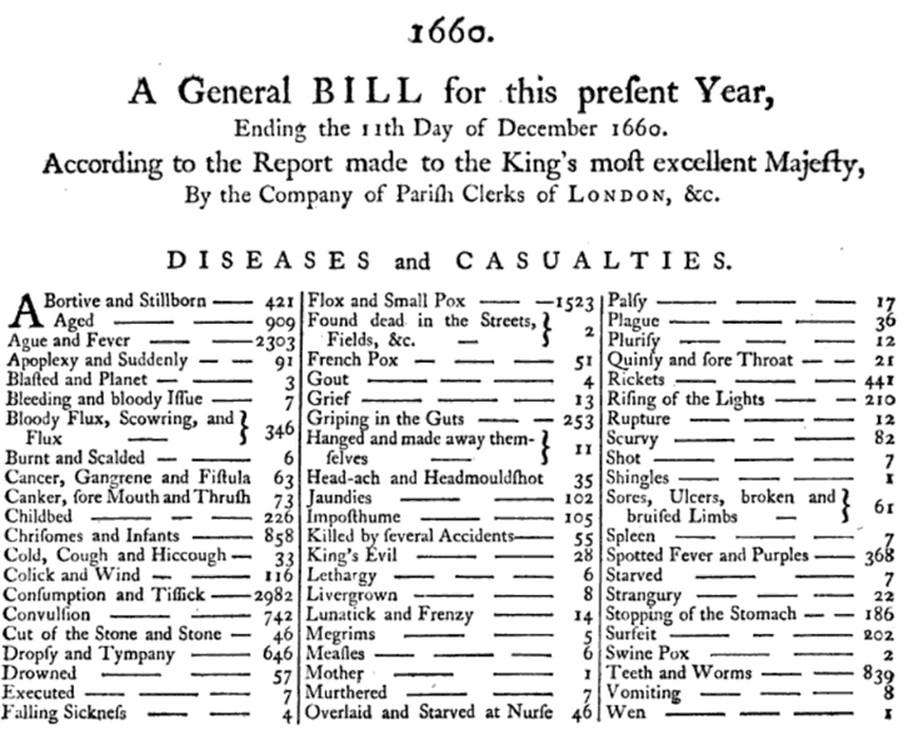
\includegraphics[width=1\linewidth]{images/StandardizedVocabularies/bill} 

}

\caption{1660 London Bill of Mortality, showing the cause of death for deceased inhabitants using a classification system of 62 diseases known at the time.}\label{fig:bill}
\end{figure}

Depuis lors, les classifications ont considérablement augmenté en taille et en complexité et se sont étendues à d'autres aspects des soins de santé, tels que les procédures et services, les médicaments, les dispositifs médicaux, etc. Les principes de base sont restés les mêmes : ce sont des vocabulaires contrôlés, des terminologies, des hiérarchies ou des ontologies qu'une certaine communauté de soins de santé accepte dans le but de capturer, de classer et d'analyser les données des patients. Bon nombre de ces vocabulaires sont maintenus par des agences publiques et gouvernementales ayant un mandat à long terme pour ce faire. Par exemple, l'Organisation mondiale de la Santé (OMS) produit la Classification Internationale des Maladies (ICD) avec l'ajout récent de sa 11e révision (ICD11). Les gouvernements locaux créent des versions spécifiques à chaque pays, telles que ICD10CM (États-Unis), ICD10GM (Allemagne), etc. Les gouvernements contrôlent également la commercialisation et la vente de médicaments et maintiennent des répertoires nationaux de ces médicaments certifiés. Les vocabulaires sont également utilisés dans le secteur privé, soit comme produits commerciaux, soit pour un usage interne, tels que les systèmes de dossiers de santé électroniques (EHR) ou pour les déclarations de sinistres d'assurance maladie.

En conséquence, chaque pays, région, système de soins de santé et institution tend à avoir ses propres classifications qui ne seraient probablement pertinentes que là où elles sont utilisées. Cette myriade de vocabulaires empêche l'interopérabilité des systèmes dans lesquels ils sont utilisés. La standardisation est la clé qui permet l'échange de données des patients, ouvre l'analyse des données de santé à un niveau mondial et permet une recherche systématique et standardisée, y compris la caractérisation des performances et l'évaluation de la qualité. Pour résoudre ce problème, des organisations multinationales ont vu le jour et ont commencé à créer des normes étendues, telles que l'OMS mentionnée ci-dessus et la Nomenclature standard de la médecine (SNOMED) ou les Identifiants et codes logiques d'observation (LOINC). Aux États-Unis, le Comité des normes informatiques de santé (HITAC) recommande l'utilisation de SNOMED, LOINC et du vocabulaire des médicaments RxNorm comme normes au Coordinateur national de l'informatique de santé (ONC) pour utilisation dans une plate-forme commune pour l'échange d'informations sanitaires à l'échelle nationale entre divers organismes.

OHDSI a développé le CDM OMOP, une norme mondiale pour la recherche observationnelle. Dans le cadre du CDM, les Vocabulaire normalisé OMOP sont disponibles à deux fins principales :

\begin{itemize}
\tightlist
\item
  Référentiel commun de tous les vocabulaires utilisés dans la communauté
\item
  Standardisation et cartographie pour une utilisation en recherche
\end{itemize}

Les Vocabulaire normalisé sont disponibles pour la communauté gratuitement et \textbf{doivent être utilisés} pour l'instance CDM OMOP \textbf{comme sa table de référence obligatoire}.

\subsection{Construire les Vocabulaire normalisé}\label{construire-les-vocabulaire-normalisuxe9}

Tous les vocabulaires des Vocabulaire normalisé sont consolidés dans le même format commun. Cela soulage les chercheurs de la nécessité de comprendre et de manipuler plusieurs formats différents et des conventions de cycle de vie des vocabulaires d'origine. Tous les vocabulaires sont régulièrement rafraîchis et incorporés en utilisant le système Pallas.\footnote{\url{https://github.com/OHDSI/Vocabulary-v5.0}} Il est construit et géré par l'équipe des vocabulaires OHDSI, qui fait partie du groupe de travail général CDM OMOP. Si vous trouvez des erreurs, veuillez les signaler et aider à améliorer notre ressource en postant sur les forums OHDSI\footnote{\url{https://forums.ohdsi.org}} ou sur la page Github du CDM.\footnote{\url{https://github.com/OHDSI/CommonDataModel/issues}} \index{Pallas system}

\subsection{Accès aux Vocabulaire normalisé}\label{accessVocabularies}

Pour obtenir les Vocabulaire normalisé, vous n'avez pas besoin d'exécuter Pallas vous-même. Au lieu de cela, vous pouvez télécharger la dernière version d'ATHENA\footnote{\url{http://athena.ohdsi.org}} et la charger dans votre base de données locale. ATHENA permet également une recherche facettée des Vocabulaires. \index{ATHENA} \index{vocabulaire normalisé!télécharger} \index{vocabulaire normalisé!recherche}

Pour télécharger un fichier zip contenant toutes les tables des Vocabulaire normalisé, sélectionnez tous les vocabulaires dont vous avez besoin pour votre CDM OMOP. Les vocabulaires avec Concepts standard (voir Section \ref{standardConcepts}) et utilisation très courante sont pré-sélectionnés. Ajoutez les vocabulaires utilisés dans vos données sources. Les vocabulaires propriétaires n'ont pas de bouton de sélection. Cliquez sur le bouton « Licence requise » pour incorporer un tel vocabulaire dans votre liste. L'équipe de vocabulaire vous contactera, vous demandera de démontrer votre licence ou vous aidera à prendre contact avec les bonnes personnes pour en obtenir une.

\subsection{Source des vocabulaires : Adopter ou Construire}\label{source-des-vocabulaires-adopter-ou-construire}

OHDSI préfère généralement adopter des vocabulaires existants, plutôt que de les construire de novo, car (i) de nombreux vocabulaires ont déjà été utilisés dans des données observationnelles dans la communauté, et (ii) la construction et la maintenance de vocabulaires est complexe et nécessite l'apport de nombreuses parties prenantes sur de longues périodes pour arriver à maturité. Pour cette raison, des organisations dédiées fournissent des vocabulaires, qui sont soumis à un cycle de vie de génération, dépréciation, fusion et scission (voir Section \ref{conceptLifeCycle}). Actuellement, OHDSI ne produit que des vocabulaires administratifs internes comme les Types de Concepts (par ex. concepts de type de condition). La seule exception est l'Extension RxNorm, un vocabulaire couvrant les médicaments qui ne sont utilisés qu'en dehors des États-Unis (voir Section \ref{rxNormExtension}).
\#\# Concepts

Tous les événements cliniques dans le CDM OMOP sont exprimés sous forme de concepts, qui représentent la notion sémantique de chaque événement. Ils constituent les éléments de base des enregistrements de données, rendant presque toutes les tables entièrement normalisées avec quelques exceptions. Les concepts sont stockés dans la table CONCEPT (voir Figure \ref{fig:concept}). \index{concept}

\begin{figure}

{\centering 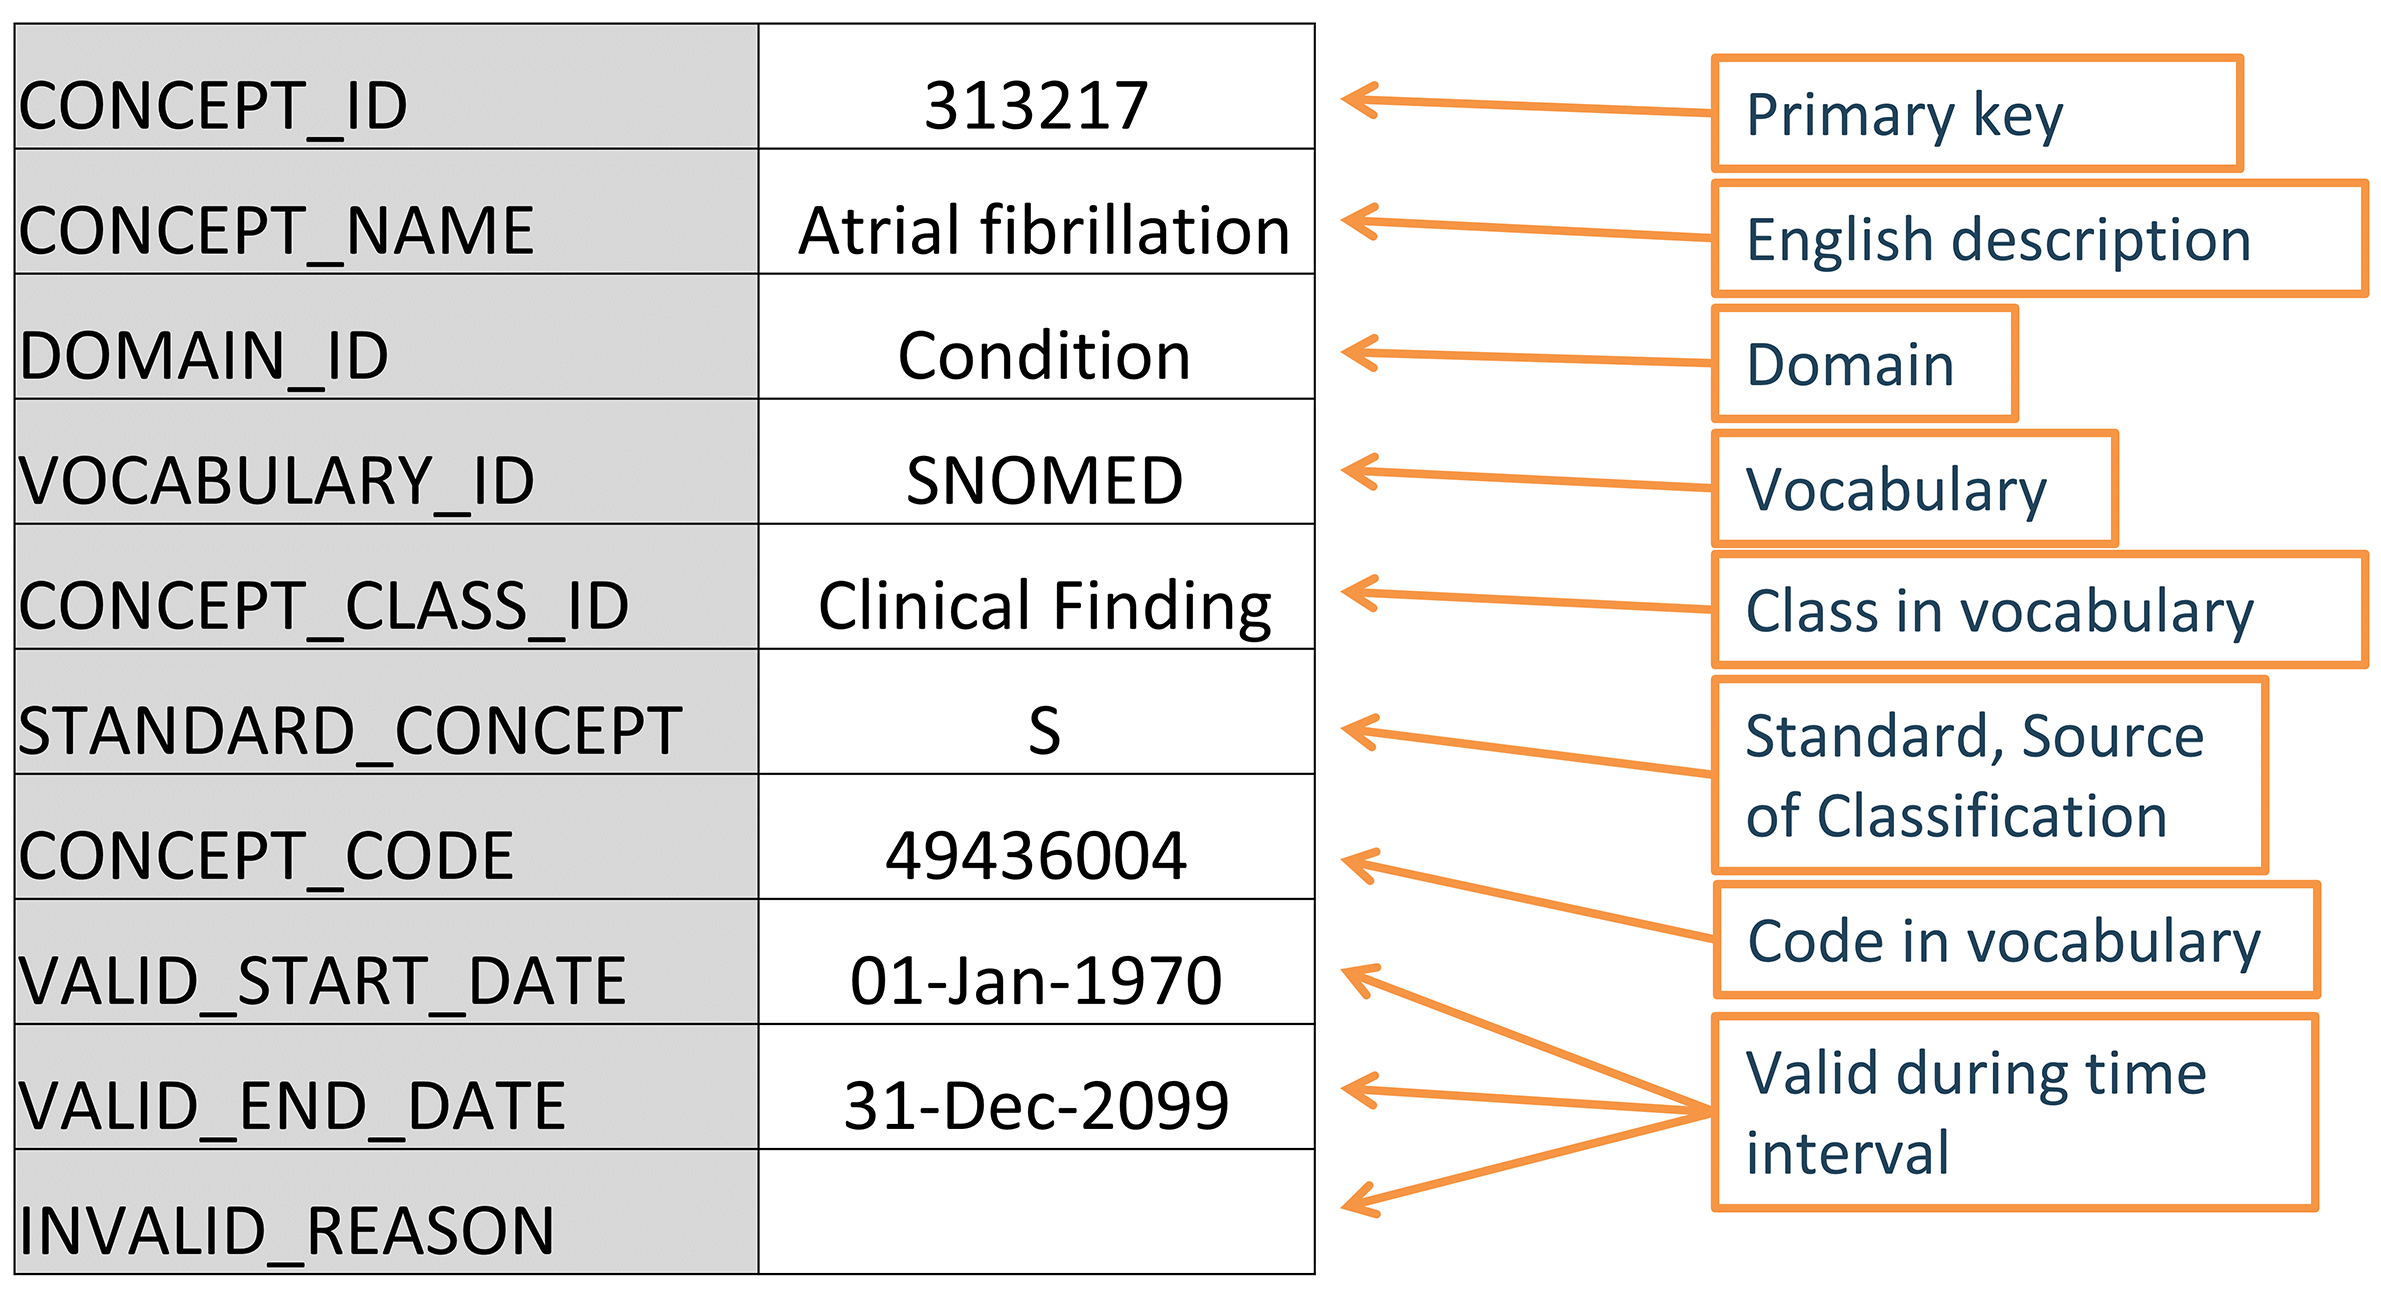
\includegraphics[width=0.9\linewidth]{images/StandardizedVocabularies/concept} 

}

\caption{Standard representation of vocabulary concepts in the OMOP CDM. The example provided is the CONCEPT table record for the SNOMED code for Atrial Fibrillation.}\label{fig:concept}
\end{figure}

Ce système se veut \textbf{complet}, c'est-à-dire qu'il existe suffisamment de concepts pour couvrir tout événement pertinent à l'expérience de soins de santé du patient (par exemple, conditions, procédures, expositions aux médicaments, etc.) ainsi que certaines informations administratives du système de santé (par exemple, visites, sites de soins, etc.).

\subsection{Identifiants de concepts}\label{identifiants-de-concepts}

Chaque concept se voit attribuer un identifiant de concept à utiliser comme clé primaire. Cet identifiant entier sans signification, plutôt que le code original du vocabulaire, est utilisé pour enregistrer des données dans les tables d'événements du CDM. \index{concept!identifier}

\subsection{Noms de concepts}\label{noms-de-concepts}

Chaque concept a un nom. Les noms sont toujours en anglais. Ils sont importés de la source du vocabulaire. Si le vocabulaire source a plus d'un nom, le plus expressif est sélectionné et les autres sont stockés dans la table CONCEPT\_SYNONYM sous la même clé CONCEPT\_ID. Les noms non anglais sont également enregistrés dans CONCEPT\_SYNONYM, avec l'identifiant de concept linguistique approprié dans le champ LANGUAGE\_CONCEPT\_ID. Le nom mesure 255 caractères de long, ce qui signifie que les noms très longs sont tronqués et la version complète est enregistrée comme un autre synonyme, pouvant contenir jusqu'à 1000 caractères.

\subsection{Domaines}\label{conceptDomains}

Chaque concept se voit attribuer un domaine dans le champ DOMAIN\_ID, qui contrairement à l'identifiant numérique CONCEPT\_ID, est un identifiant alphanumérique court, sensible à la casse et unique pour le domaine. Des exemples de ces identifiants de domaine sont ``Condition'', ``Drug'', ``Procedure'', ``Visit'', ``Device'', ``Specimen'', etc. Les concepts ambigus ou pré-coordonnés (combinaison) peuvent appartenir à un domaine combiné, mais les Concepts Standards (voir Section \ref{standardConcepts}) sont toujours assignés à un domaine unique. Les domaines indiquent également dans quelle table et champ du CDM un événement clinique ou un attribut d'événement est enregistré. Les affectations de domaine sont une caractéristique spécifique à OMOP effectuée lors de l'ingestion de vocabulaire en utilisant une heuristique décrite dans \href{https://github.com/ohDSI/vocabulary-v5.0}{Pallas}. Les vocabulaires sources tendent à combiner des codes de domaines mixtes, mais à des degrés divers (voir Figure \ref{fig:domains}). \index{domain!concept}

\begin{figure}

{\centering 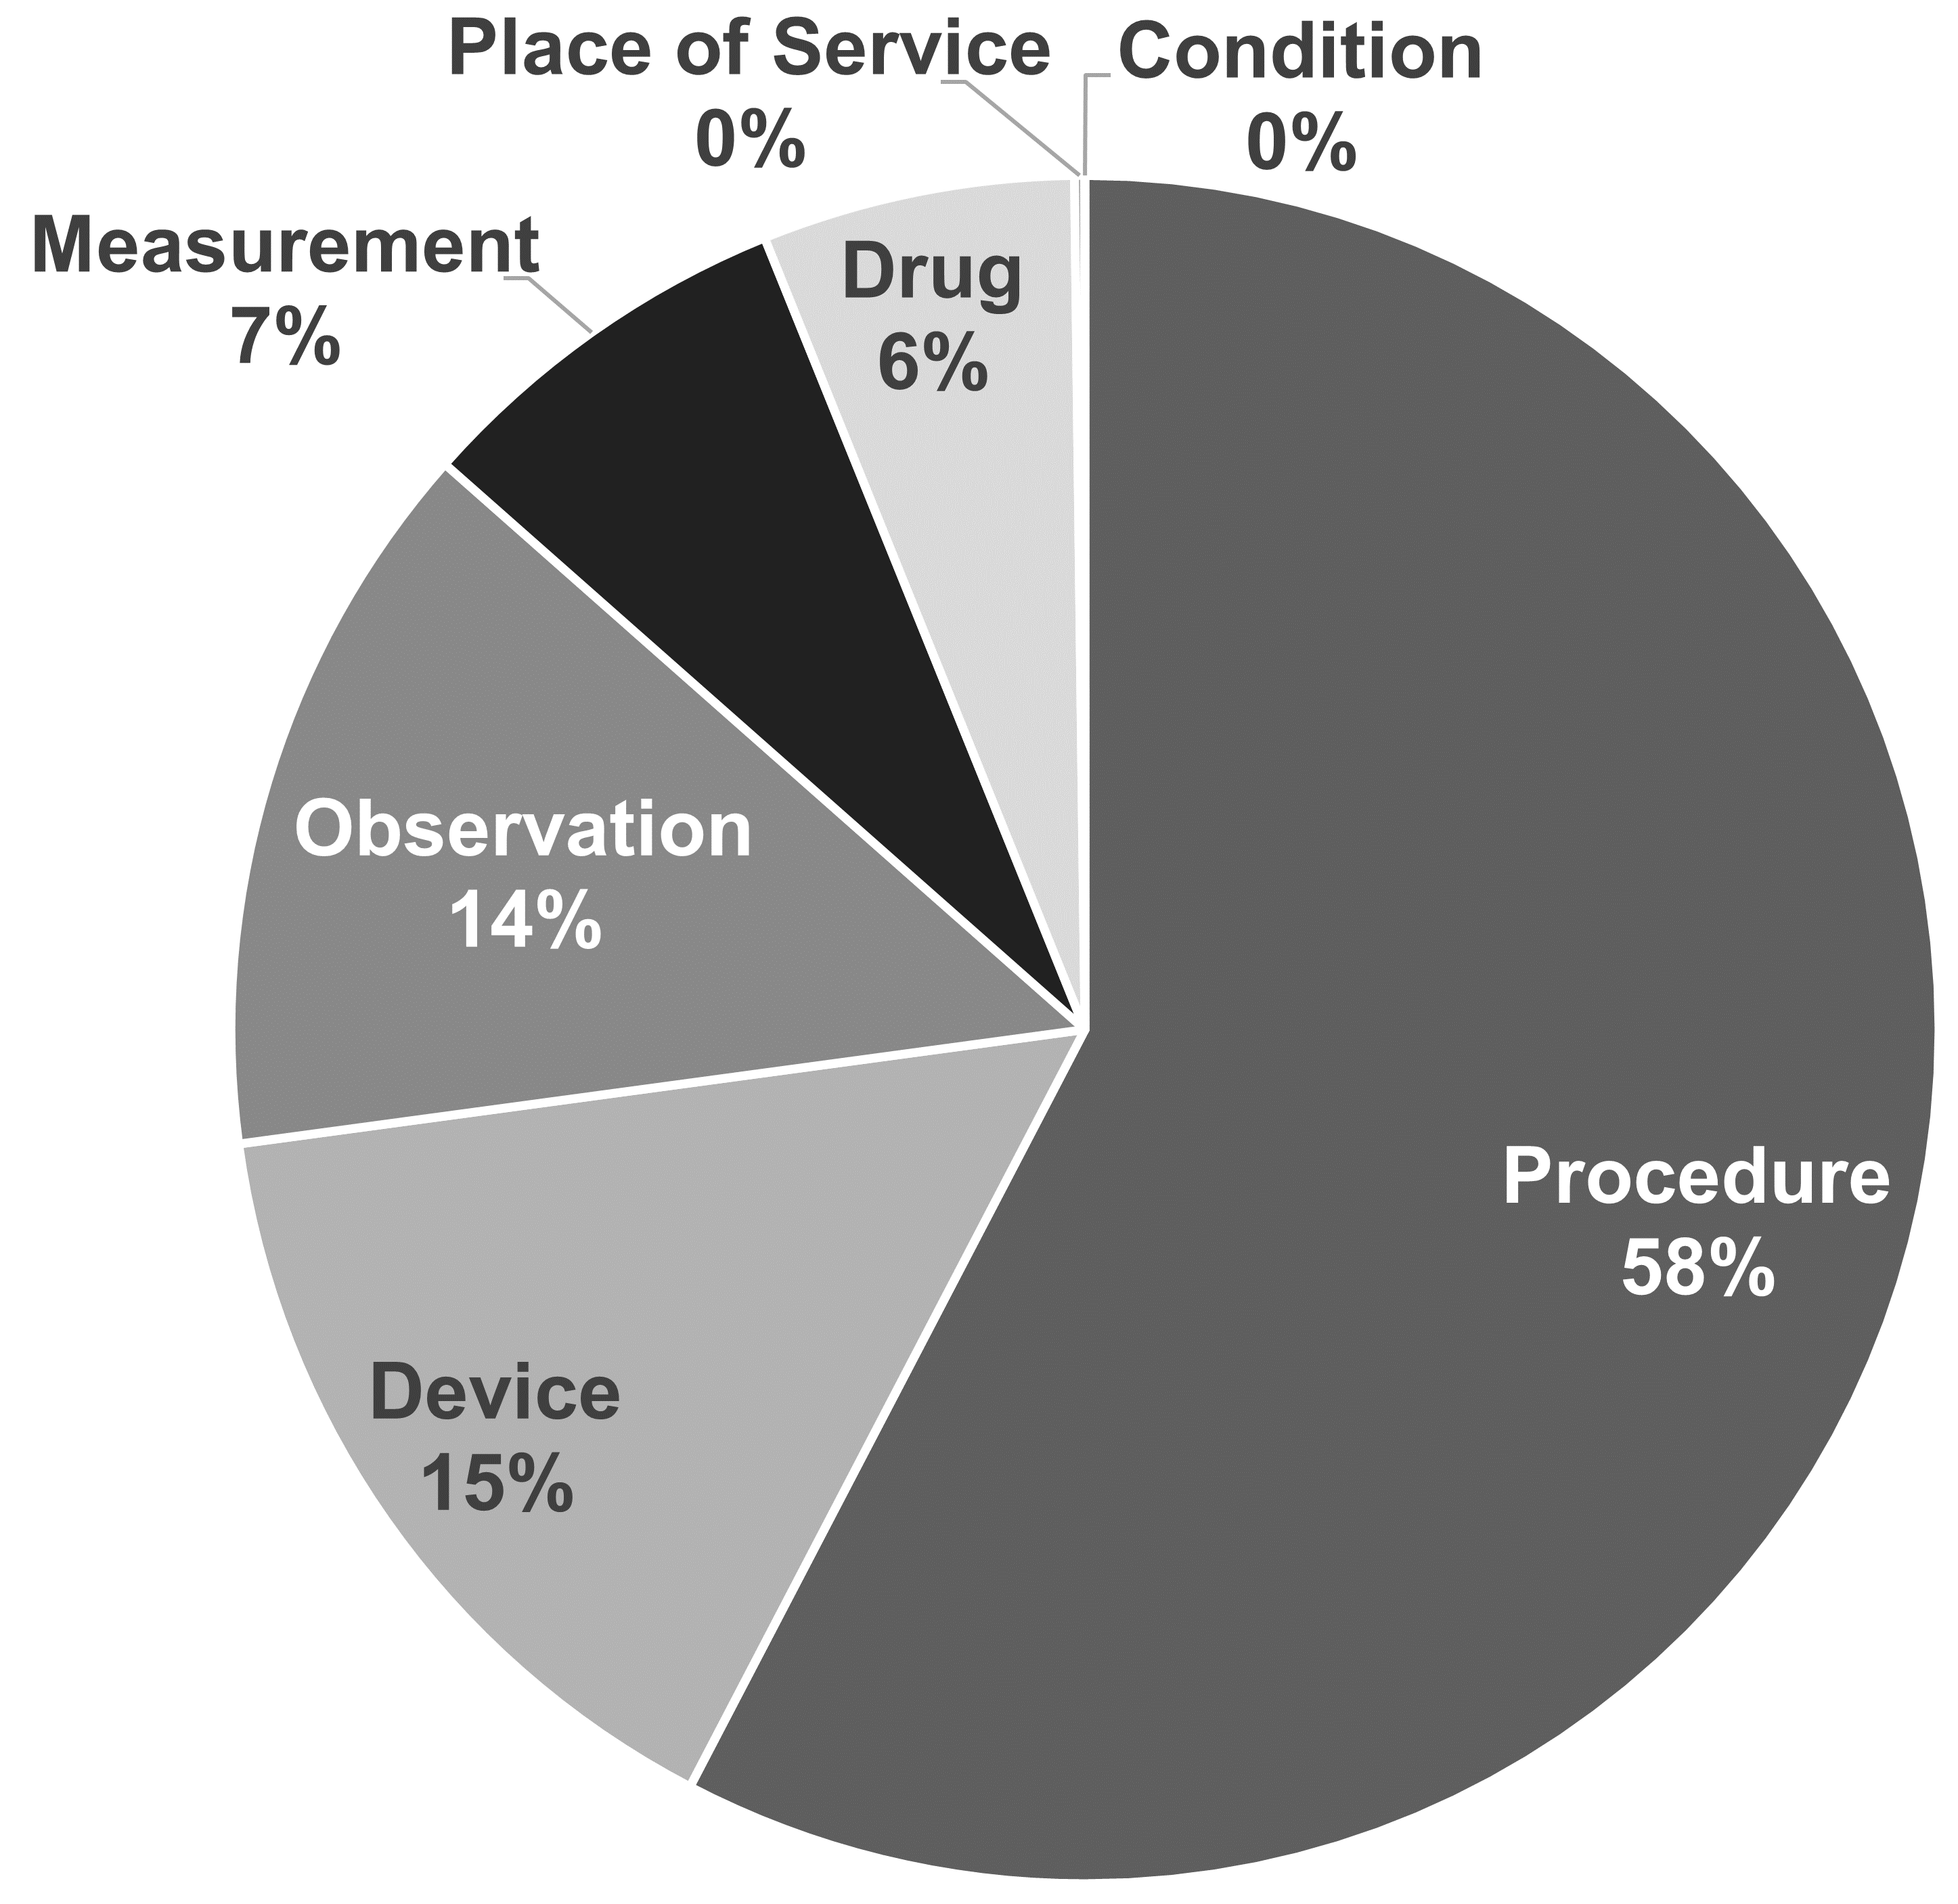
\includegraphics[width=0.7\linewidth]{images/StandardizedVocabularies/domains} 

}

\caption{Domain assignment in procedure vocabularies CPT4 and HCPCS. By intuition, these vocabularies should contain codes and concepts of a single domain, but in reality they are mixed.}\label{fig:domains}
\end{figure}

L'heuristique de domaine suit les définitions des domaines. Ces définitions sont dérivées des définitions des tables et des champs dans le CDM (voir Chapitre \ref{CommonDataModel}). L'heuristique n'est pas parfaite ; il y a des zones grises (voir Section \ref{specialSituations} ``Situations spéciales''). Si vous trouvez des domaines de concepts assignés incorrectement, veuillez le signaler et aider à améliorer le processus via un post sur le \href{https://forums.ohdsi.org}{Forums} ou un \href{https://github.com/OHDSI/CommonDataModel/issues}{CDM issue}.

\subsection{Vocabulaires}\label{vocabulaires}

Chaque vocabulaire a un identifiant alphanumérique court, sensible à la casse et unique, qui suit généralement le nom abrégé du vocabulaire, en omettant les tirets. Par exemple, ICD-9-CM a l'identifiant de vocabulaire ``ICD9CM''. Il y a actuellement 111 vocabulaires pris en charge par OHDSI, dont 78 sont adoptés de sources externes, tandis que le reste sont des vocabulaires internes OMOP. Ces vocabulaires sont généralement mis à jour selon un calendrier trimestriel. La source et la version des vocabulaires sont définies dans le fichier de référence VOCABULARY. \index{vocabulary}

\subsection{Classes de concepts}\label{classes-de-concepts}

Certains vocabulaires classifient leurs codes ou concepts, indiqués par leurs identifiants alphanumériques uniques et sensibles à la casse. Par exemple, SNOMED a 33 de ces classes de concepts, que SNOMED appelle ``balises sémantiques'' : constatation clinique, contexte social, structure corporelle, etc. Ce sont des divisions verticales des concepts. D'autres, tels que MedDRA ou RxNorm, ont des classes de concepts classifiant les niveaux horizontaux dans leurs hiérarchies stratifiées. Les vocabulaires sans aucune classe de concepts, comme HCPCS, utilisent l'identifiant de vocabulaire comme identifiant de classe de concepts. \index{concept!class}

\begin{longtable}[]{@{}
  >{\raggedright\arraybackslash}p{(\columnwidth - 2\tabcolsep) * \real{0.2045}}
  >{\raggedright\arraybackslash}p{(\columnwidth - 2\tabcolsep) * \real{0.7955}}@{}}
\caption{\label{tab:sublassification} Vocabulaires avec ou sans principes de sous-classement horizontal et vertical dans la classe de concepts.}\tabularnewline
\toprule\noalign{}
\begin{minipage}[b]{\linewidth}\raggedright
Principe de subdivision de la classe de concepts
\end{minipage} & \begin{minipage}[b]{\linewidth}\raggedright
Vocabulaire
\end{minipage} \\
\midrule\noalign{}
\endfirsthead
\toprule\noalign{}
\begin{minipage}[b]{\linewidth}\raggedright
Principe de subdivision de la classe de concepts
\end{minipage} & \begin{minipage}[b]{\linewidth}\raggedright
Vocabulaire
\end{minipage} \\
\midrule\noalign{}
\endhead
\bottomrule\noalign{}
\endlastfoot
Horizontal & tous les vocabulaires de médicaments, ATC, CDT, épisode, HCPCS, HemOnc, ICDs, MedDRA, OSM, Recensement \\
Vertical & CIEL, HES Specialty, ICDO3, MeSH, NAACCR, NDFRT, OPCS4, PCORNET, Plan, PPI, Fournisseur, SNOMED, SPL, UCUM \\
Mixte & CPT4, ISBT, LOINC \\
Aucun & APC, tous les concepts de type, Ethnicity, OXMIS, Race, Revenue Code, Sponsor, Supplier, UB04s, Visit \\
\end{longtable}

Les classes de concepts horizontales vous permettent de déterminer un niveau hiérarchique spécifique. Par exemple, dans le vocabulaire des médicaments RxNorm, la classe de concepts ``Ingrédient'' définit le niveau supérieur de la hiérarchie. Dans le modèle vertical, les membres d'une classe de concepts peuvent être de n'importe quel niveau hiérarchique du haut vers le bas.

\subsection{Concepts standards}\label{standardConcepts}

Un concept représentant le sens de chaque événement clinique est désigné Standard. Par exemple, le code MESH D001281, le code CIEL 148203, le code SNOMED 49436004, le code ICD9CM 427.31 et le code Read G573000 définissent tous ``fibrillation auriculaire'' dans le domaine de la condition, mais uniquement le concept SNOMED est Standard et représente la condition dans les données. Les autres sont désignés concepts non standards ou sources et mappés aux concepts standards. Les concepts standards sont indiqués par un ``S'' dans le champ STANDARD\_CONCEPT. Et seuls ces Concepts Standards sont utilisés pour enregistrer des données dans les champs CDM se terminant par ``\_CONCEPT\_ID''. \index{standard concept}

\subsection{Concepts non standards}\label{concepts-non-standards}

Les concepts non standards ne sont pas utilisés pour représenter les événements cliniques, mais ils font toujours partie des vocabulaires standardisés, et se trouvent souvent dans les données sources. Pour cette raison, ils sont également appelés ``concepts sources''. La conversion des concepts sources en Concepts Standards est un processus appelé ``mapping'' (voir Section \ref{conceptMapping}). Les concepts non standards n'ont aucune valeur (NULL) dans le champ STANDARD\_CONCEPT.

\subsection{Concepts de classification}\label{concepts-de-classification}

Ces concepts ne sont pas standards et ne peuvent donc pas être utilisés pour représenter les données. Mais ils participent à la hiérarchie avec les Concepts Standards, et peuvent donc être utilisés pour effectuer des requêtes hiérarchiques. Par exemple, interroger tous les descendants du code MedDRA 10037908 (non visible pour les utilisateurs qui n'ont pas obtenu une licence MedDRA, voir Section \ref{accessVocabularies} pour les restrictions d'accès) récupérera le concept SNOMED standard pour la fibrillation auriculaire (voir Section \ref{conceptAncestor} pour des requêtes hiérarchiques utilisant la table CONCEPT\_ANCESTOR) - voir Figure \ref{fig:hierarchy}. \index{classification concept}

\begin{figure}

{\centering 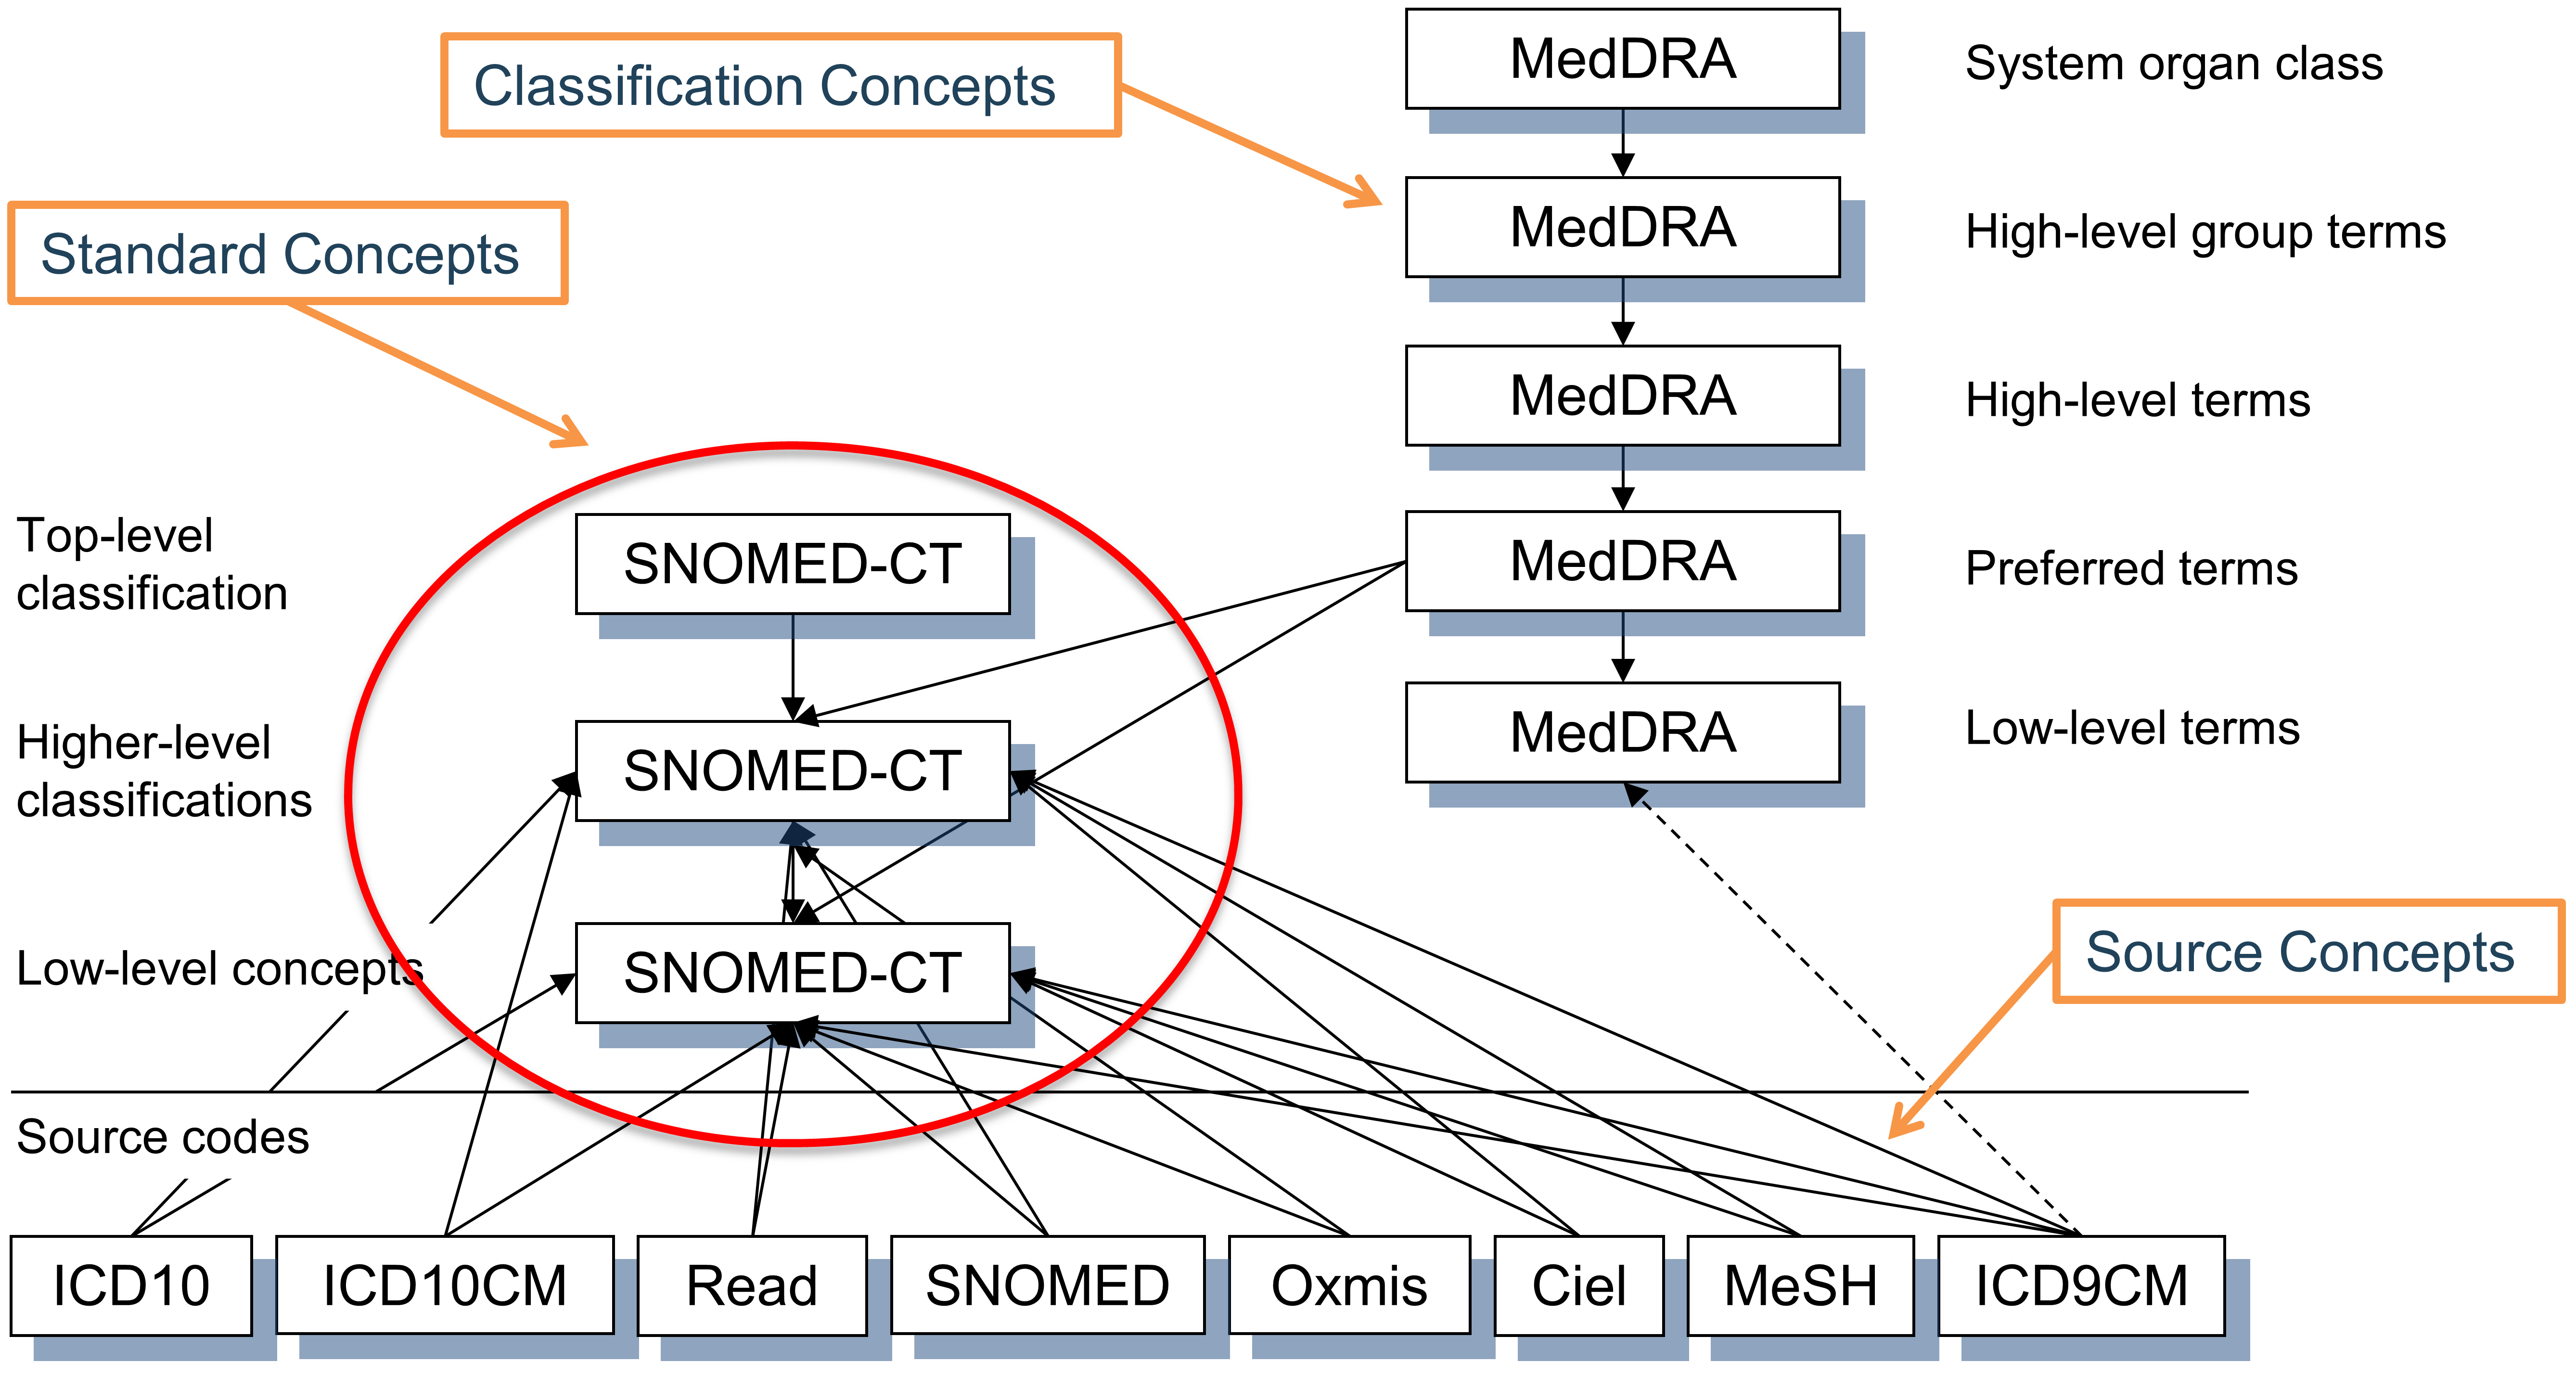
\includegraphics[width=1\linewidth]{images/StandardizedVocabularies/hierarchy} 

}

\caption{Standard, non-standard source and classification concepts and their hierarchical relationships in the condition domain. SNOMED is used for most standard condition concepts (with some oncology-related concepts derived from ICDO3), MedDRA concepts are used for hierarchical classification concepts, and all other vocabularies contain non-standard or source concepts, which do not participate in the hierarchy.}\label{fig:hierarchy}
\end{figure}

Le choix de la désignation des concepts en tant que Standard, non standard et classification est généralement fait pour chaque domaine séparément au niveau du vocabulaire. Cela est basé sur la qualité des concepts, la hiérarchie intégrée et le but déclaré du vocabulaire. De plus, tous les concepts d'un vocabulaire ne sont pas utilisés comme Concepts Standards. La désignation est séparée pour chaque domaine, chaque concept doit être actif (voir Section \ref{conceptLifeCycle}) et il peut y avoir un ordre de préséance si plus d'un concept de différents vocabulaires sont en concurrence pour le même sens. En d'autres termes, il n'existe pas de ``vocabulaire standard''. Voir Table \ref{tab:vocabList} pour des exemples.

\begin{longtable}[]{@{}
  >{\raggedright\arraybackslash}p{(\columnwidth - 6\tabcolsep) * \real{0.1636}}
  >{\raggedright\arraybackslash}p{(\columnwidth - 6\tabcolsep) * \real{0.2909}}
  >{\raggedright\arraybackslash}p{(\columnwidth - 6\tabcolsep) * \real{0.2909}}
  >{\raggedright\arraybackslash}p{(\columnwidth - 6\tabcolsep) * \real{0.2545}}@{}}
\caption{\label{tab:vocabList} Liste des vocabulaires à utiliser pour les affectations de concepts standards/non standards/de classification.}\tabularnewline
\toprule\noalign{}
\begin{minipage}[b]{\linewidth}\raggedright
Domaine
\end{minipage} & \begin{minipage}[b]{\linewidth}\raggedright
pour Concepts Standards
\end{minipage} & \begin{minipage}[b]{\linewidth}\raggedright
pour concepts sources
\end{minipage} & \begin{minipage}[b]{\linewidth}\raggedright
pour concepts de classification
\end{minipage} \\
\midrule\noalign{}
\endfirsthead
\toprule\noalign{}
\begin{minipage}[b]{\linewidth}\raggedright
Domaine
\end{minipage} & \begin{minipage}[b]{\linewidth}\raggedright
pour Concepts Standards
\end{minipage} & \begin{minipage}[b]{\linewidth}\raggedright
pour concepts sources
\end{minipage} & \begin{minipage}[b]{\linewidth}\raggedright
pour concepts de classification
\end{minipage} \\
\midrule\noalign{}
\endhead
\bottomrule\noalign{}
\endlastfoot
Condition & SNOMED, ICDO3 & SNOMED Veterinary & MedDRA \\
Procédure & SNOMED, CPT4, HCPCS, ICD10PCS, ICD9Proc, OPCS4 & SNOMED Veterinary, HemOnc, NAACCR & Aucun pour le moment \\
Mesure & SNOMED, LOINC & SNOMED Veterinary, NAACCR, CPT4, HCPCS, OPCS4, PPI & Aucun pour le moment \\
Médicament & RxNorm, RxNorm Extension, CVX & HCPCS, CPT4, HemOnc, NAAACCR & ATC \\
Dispositif & SNOMED & Autres, actuellement non normalisés & Aucun pour le moment \\
Observation & SNOMED & Autres & Aucun pour le moment \\
Visite & CMS Place of Service, ABMT, NUCC & SNOMED, HCPCS, CPT4, UB04 & Aucun pour le moment \\
\end{longtable}

\subsection{Codes de concepts}\label{codes-de-concepts}

Les codes de concepts sont les identifiants utilisés dans les vocabulaires sources. Par exemple, les codes ICD9CM ou NDC sont stockés dans ce champ, tandis que les tables OMOP utilisent l'identifiant de concept comme clé étrangère dans la table CONCEPT. La raison est que l'espace de noms chevauche les vocabulaires, c'est-à-dire que le même code peut exister dans différents vocabulaires avec des significations complètement différentes (voir Table \ref{tab:code1001}) \index{concept!code}

\begin{longtable}[]{@{}
  >{\raggedright\arraybackslash}p{(\columnwidth - 10\tabcolsep) * \real{0.1639}}
  >{\raggedright\arraybackslash}p{(\columnwidth - 10\tabcolsep) * \real{0.0820}}
  >{\raggedright\arraybackslash}p{(\columnwidth - 10\tabcolsep) * \real{0.2131}}
  >{\raggedright\arraybackslash}p{(\columnwidth - 10\tabcolsep) * \real{0.1803}}
  >{\raggedright\arraybackslash}p{(\columnwidth - 10\tabcolsep) * \real{0.1803}}
  >{\raggedright\arraybackslash}p{(\columnwidth - 10\tabcolsep) * \real{0.1803}}@{}}
\caption{\label{tab:code1001} Concepts avec un code de concept identique 1001, mais des vocabulaires, des domaines et des classes de concepts différents.}\tabularnewline
\toprule\noalign{}
\begin{minipage}[b]{\linewidth}\raggedright
Concept ID
\end{minipage} & \begin{minipage}[b]{\linewidth}\raggedright
Concept Code
\end{minipage} & \begin{minipage}[b]{\linewidth}\raggedright
Concept Name
\end{minipage} & \begin{minipage}[b]{\linewidth}\raggedright
Domain ID
\end{minipage} & \begin{minipage}[b]{\linewidth}\raggedright
Vocabulary ID
\end{minipage} & \begin{minipage}[b]{\linewidth}\raggedright
Concept Class
\end{minipage} \\
\midrule\noalign{}
\endfirsthead
\toprule\noalign{}
\begin{minipage}[b]{\linewidth}\raggedright
Concept ID
\end{minipage} & \begin{minipage}[b]{\linewidth}\raggedright
Concept Code
\end{minipage} & \begin{minipage}[b]{\linewidth}\raggedright
Concept Name
\end{minipage} & \begin{minipage}[b]{\linewidth}\raggedright
Domain ID
\end{minipage} & \begin{minipage}[b]{\linewidth}\raggedright
Vocabulary ID
\end{minipage} & \begin{minipage}[b]{\linewidth}\raggedright
Concept Class
\end{minipage} \\
\midrule\noalign{}
\endhead
\bottomrule\noalign{}
\endlastfoot
35803438 & 1001 & Granulocyte colony-stimulating factors & Drug & HemOnc & Component Class \\
35942070 & 1001 & AJCC TNM Clin T & Measurement & NAACCR & NAACCR Variable \\
1036059 & 1001 & Antipyrine & Drug & RxNorm & Ingredient \\
38003544 & 1001 & Residential Treatment - Psychiatric & Revenue Code & Revenue Code & Revenue Code \\
43228317 & 1001 & Aceprometazine maleate & Drug & BDPM & Ingredient \\
45417187 & 1001 & Brompheniramine Maleate, 10 mg/mL injectable solution & Drug & Multum & Multum \\
45912144 & 1001 & Serum & Specimen & CIEL & Specimen \\
\end{longtable}

\subsection{Cycle de vie}\label{conceptLifeCycle}

Les vocabulaires sont rarement des corpus permanents avec un ensemble fixe de codes. Au contraire, des codes et des concepts sont ajoutés et sont dépréciés. Le CDM OMOP est un modèle pour soutenir les données patient longitudinales, ce qui signifie qu'il doit prendre en charge les concepts qui étaient utilisés dans le passé et qui peuvent ne plus être actifs, ainsi que prendre en charge de nouveaux concepts et les replacer dans leur contexte. Il existe trois champs dans la table CONCEPT qui décrivent les statuts possibles du cycle de vie : VALID\_START\_DATE, VALID\_END\_DATE, et INVALID\_REASON. Leurs valeurs diffèrent selon le statut du cycle de vie du concept :

\begin{itemize}
\tightlist
\item
  \textbf{Concept actif ou nouveau}

  \begin{itemize}
  \tightlist
  \item
    Description : Concept utilisé.
  \item
    VALID\_START\_DATE : Jour de l'instanciation du concept, si cela n'est pas connu jour d'incorporation du concept dans les Vocabulaires, si cela n'est pas connu 1970-1-1.
  \item
    VALID\_END\_DATE : Fixé au 2099-12-31 comme convention pour indiquer ``Peut devenir invalide dans un futur indéfini, mais actif pour le moment''.
  \item
    INVALID\_REASON : NULL
  \end{itemize}
\item
  \textbf{Concept déprécié sans successeur}

  \begin{itemize}
  \tightlist
  \item
    Description : Concept inactif et ne peut pas être utilisé comme Standard (voir Section \ref{standardConcepts}).
  \item
    VALID\_START\_DATE : Jour de l'instanciation du concept, si cela n'est pas connu jour d'incorporation du concept dans les Vocabulaires, si cela n'est pas connu 1970-1-1.
  \item
    VALID\_END\_DATE : Jour dans le passé indiquant la dépréciation, ou si cela n'est pas connu jour de mise à jour du vocabulaire où le concept dans le vocabulaire a disparu ou a été mis à inactif.
  \item
    INVALID\_REASON : ``D''
  \end{itemize}
\item
  \textbf{Concept mis à jour avec successeur}

  \begin{itemize}
  \tightlist
  \item
    Description : Concept inactif, mais a un successeur défini. Il s'agit généralement de concepts qui ont subi une déduplication.
  \item
    VALID\_START\_DATE : Jour de l'instanciation du concept, si cela n'est pas connu jour d'incorporation du concept dans les Vocabulaires, si cela n'est pas connu 1970-1-1.
  \item
    VALID\_END\_DATE : Jour dans le passé indiquant une mise à jour, ou si cela n'est pas connu jour de mise à jour du vocabulaire où la mise à jour a été incluse.
  \item
    INVALID\_REASON : ``U''
  \end{itemize}
\item
  \textbf{Code réutilisé pour un autre nouveau concept}

  \begin{itemize}
  \tightlist
  \item
    Description : Le vocabulaire a réutilisé le code de concept de ce concept déprécié pour un nouveau concept.
  \item
    VALID\_START\_DATE : Jour de l'instanciation du concept, si cela n'est pas connu jour d'incorporation du concept dans les Vocabulaires, si cela n'est pas connu 1970-1-1.
  \item
    VALID\_END\_DATE : Jour dans le passé indiquant la dépréciation, ou si cela n'est pas connu jour de mise à jour du vocabulaire où le concept dans le vocabulaire a disparu ou a été mis à inactif.
  \item
    INVALID\_REASON : ``R''
  \end{itemize}
\end{itemize}

En général, les codes de concepts ne sont pas réutilisés. Mais il y a quelques vocabulaires qui dévient de cette règle, en particulier HCPCS, NDC et DRG. Pour ceux-ci, le même code de concept apparaît dans plus d'un concept du même vocabulaire. Leur valeur CONCEPT\_ID reste unique. Ces codes de concepts réutilisés sont marqués par un ``R'' dans le champ INVALID\_REASON, et la période VALID\_START\_DATE à VALID\_END\_DATE doit être utilisée pour distinguer les concepts avec les mêmes codes de concepts.

\section{Relations}\label{relations}

Deux concepts quelconques peuvent avoir une relation définie, que les deux concepts appartiennent ou non au même domaine ou vocabulaire. La nature des relations est indiquée par son identifiant alphanumérique unique, sensible à la casse et court, dans le champ RELATIONSHIP\_ID de la table CONCEPT\_RELATIONSHIP. Les relations sont symétriques, c'est-à-dire que pour chaque relation existe une relation équivalente, où le contenu des champs CONCEPT\_ID\_1 et CONCEPT\_ID\_2 est échangé et le RELATIONSHIP\_ID est changé en son opposé. Par exemple, la relation ``Maps to'' a une relation opposée ``Mapped from.'' \index{concept!relation}

Les enregistrements de la table CONCEPT\_RELATIONSHIP ont également des champs de cycle de vie RELATIONSHIP\_START\_DATE, RELATIONSHIP\_END\_DATE et INVALID\_REASON. Cependant, seuls les enregistrements actifs avec INVALID\_REASON = NULL sont disponibles via ATHENA. Les relations inactives sont maintenues dans le système Pallas pour un traitement interne uniquement. La table RELATIONSHIP sert de référence avec la liste complète des identifiants de relation et leurs équivalents inversés.

\subsection{Relations de Mapping}\label{conceptMapping}

Ces relations fournissent des traductions de concepts non standard à des concepts standard, soutenues par deux paires d'identifiants de relation (voir le Tableau \ref{tab:mappingRelationships}). \index{concept!mappage}

Tableau : \label{tab:mappingRelationships} Type de relations de montage.

\begin{longtable}[]{@{}
  >{\raggedright\arraybackslash}p{(\columnwidth - 2\tabcolsep) * \real{0.2090}}
  >{\raggedright\arraybackslash}p{(\columnwidth - 2\tabcolsep) * \real{0.7910}}@{}}
\toprule\noalign{}
\begin{minipage}[b]{\linewidth}\raggedright
Paire d'identifiant de relation
\end{minipage} & \begin{minipage}[b]{\linewidth}\raggedright
Objectif
\end{minipage} \\
\midrule\noalign{}
\endhead
\bottomrule\noalign{}
\endlastfoot
``Maps to'' et ``Mapped from'' & Mapping vers les concepts standard. Les concepts standard sont mappés à eux-mêmes, les concepts non standard aux concepts standard. La plupart des concepts non standard et tous les concepts standard ont cette relation à un concept standard. Les premiers sont stockés dans les champs *\_SOURCE\_CONCEPT\_ID, et les seconds dans les champs *\_CONCEPT\_ID. Les concepts de classification ne sont pas mappés. \\
``Maps to value'' et ``Value mapped from'' & Mapping vers un concept qui représente une Valeur à placer dans les champs VALUE\_AS\_CONCEPT\_ID des tables MEASUREMENT et OBSERVATION. \\
\end{longtable}

Le but de ces relations de mapping est de permettre un rapprochement entre des concepts équivalents pour harmoniser la représentation des événements cliniques dans l'OMOP CDM. C'est une réalisation importante des vocabulaires standardisés.

``Concepts équivalents'' signifie qu'ils portent la même signification et, ce qui est important, que les descendants hiérarchiques couvrent le même espace sémantique. Si un concept équivalent n'est pas disponible et que le concept n'est pas standard, il est toujours mappé, mais vers un concept légèrement plus large (appelés ``mappings en montée''). Par exemple, l'ICD10CM W61.51 ``Mordu par une oie'' n'a pas d'équivalent dans le vocabulaire SNOMED, qui est généralement utilisé pour les concepts de condition standard. Il est donc mappé à SNOMED 217716004 ``Picoté par un oiseau,'' perdant ainsi le contexte de l'oiseau étant une oie. Les mappings en montée ne sont utilisés que si la perte d'information est jugée négligeable pour les cas d'utilisation de recherche standard.

Certains mappings connectent un concept source à plus d'un concept standard. Par exemple, ICD9CM 070.43 ``Hépatite E avec coma hépatique'' est mappé à la fois à SNOMED 235867002 ``Hépatite aiguë E'' et à SNOMED 72836002 ``Coma hépatique.'' La raison en est que le concept source original est une combinaison pré-coordonnée de deux conditions, l'hépatite et le coma. SNOMED n'a pas cette combinaison, ce qui entraîne deux enregistrements écrits pour l'enregistrement ICD9CM, chacun avec un concept standard mappé.

Les relations ``Maps to value'' ont pour objectif de diviser une valeur pour les tables OMOP CDM suivant un modèle entité-attribut-valeur (EAV). C'est typiquement le cas dans les situations suivantes :

\begin{itemize}
\tightlist
\item
  Mesures consistant en un test et un résultat
\item
  Antécédents personnels ou familiaux de maladie
\item
  Allergie à une substance
\item
  Besoin de vaccination
\end{itemize}

Dans ces situations, le concept source est une combinaison de l'attribut (test ou antécédent) et de la valeur (résultat du test ou maladie). La relation ``Maps to'' mappe cette source au concept d'attribut, et la ``Maps to value'' au concept de valeur. Voir la Figure \ref{fig:conceptValue} pour un exemple.

\begin{figure}

{\centering 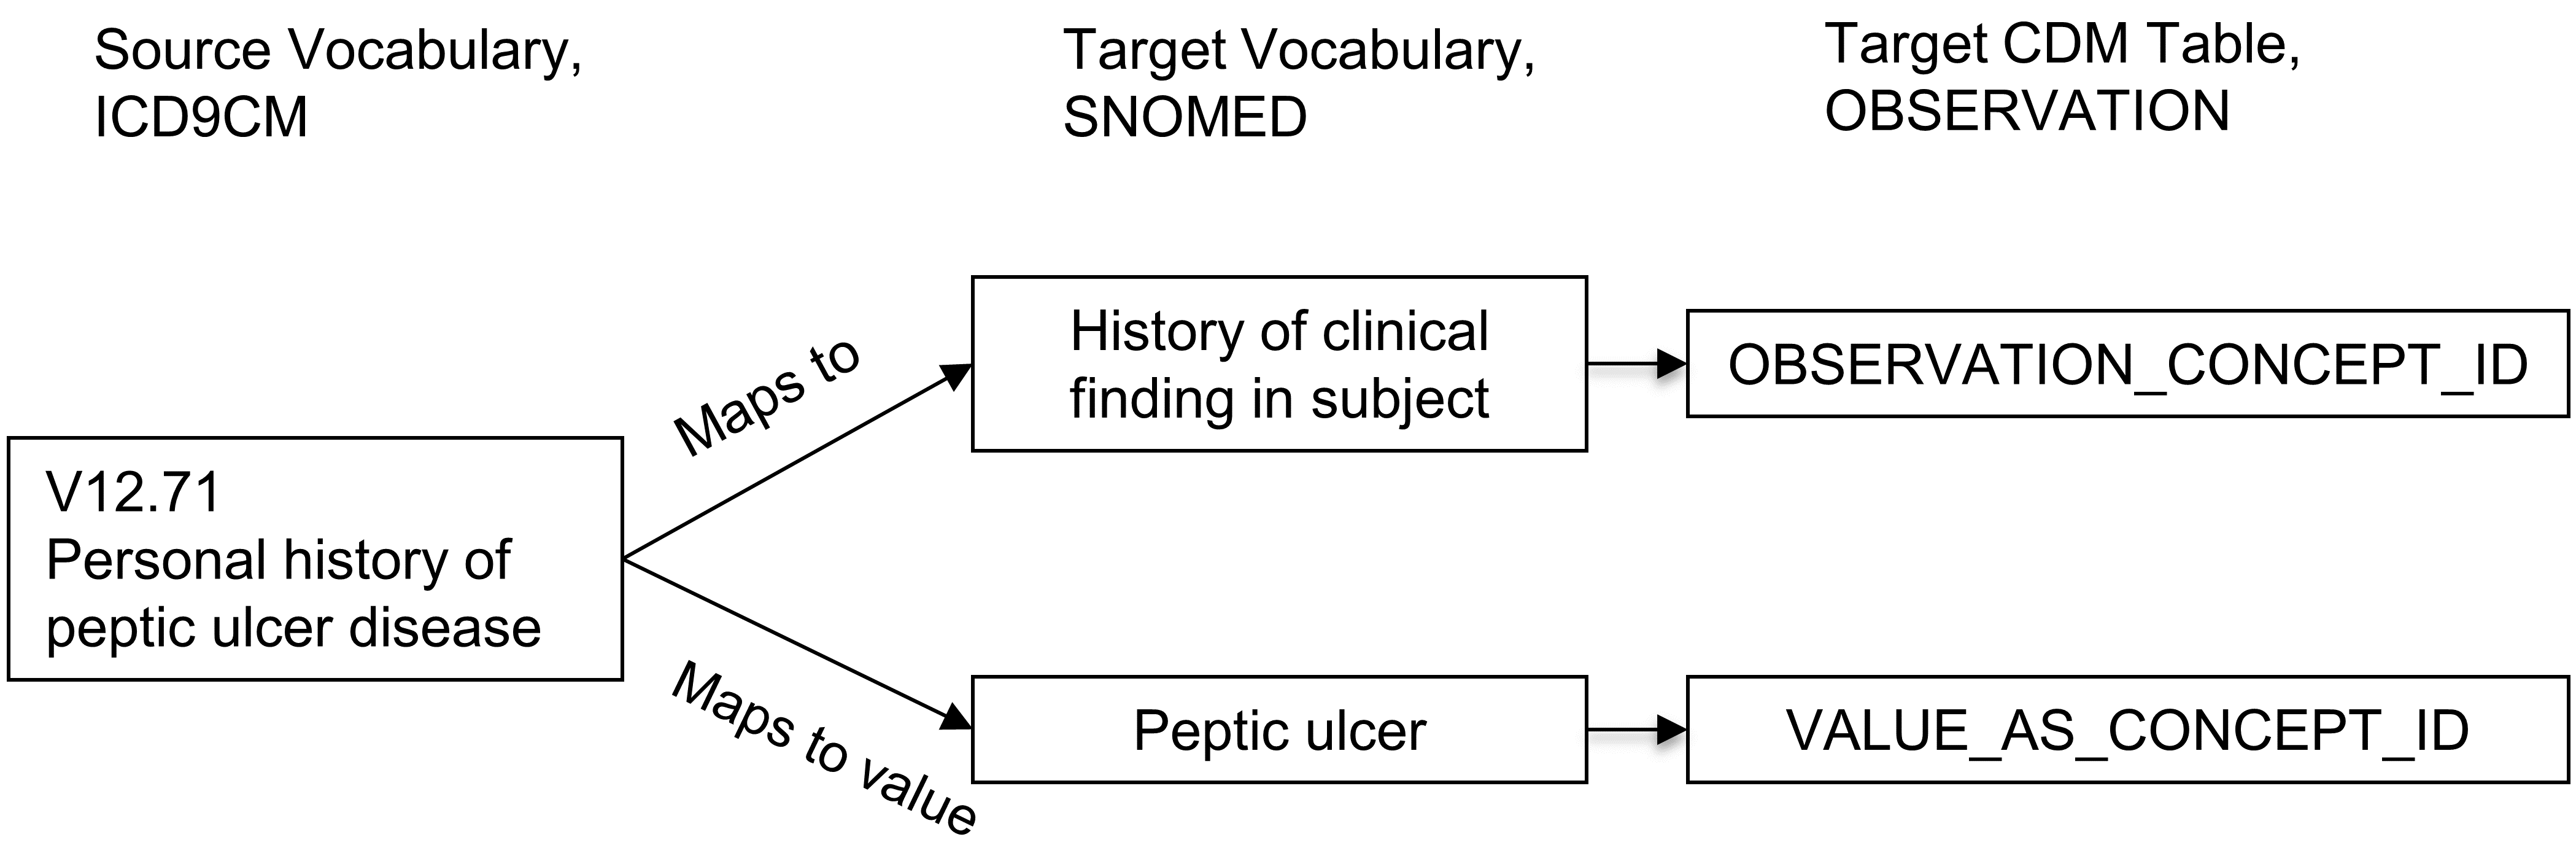
\includegraphics[width=1\linewidth]{images/StandardizedVocabularies/conceptValue} 

}

\caption{One-to-many mapping between source concept and Standard Concepts. A pre-coordinated concept is split into two concepts, one of which is the attribute (here history of clinical finding) and the other one is the value (peptic ulcer). While 'Maps to' relationship will map to concepts of the measurement or observation domains, the 'Maps to value' concepts have no domain restriction.}\label{fig:conceptValue}
\end{figure}

Le mapping des concepts est une autre caractéristique centrale des vocabulaires standardisés OMOP fournis gratuitement et soutenant les efforts de la communauté menant des études en réseau. Les relations de mapping sont dérivées de sources externes ou maintenues manuellement par l'équipe des vocabulaires. Cela signifie qu'elles ne sont pas parfaites. Si vous trouvez des relations de mapping incorrectes ou contestables, il est crucial de les signaler et d'aider à améliorer le processus via un post sur les \href{https://forums.ohdsi.org}{Forums} ou un \href{https://github.com/OHDSI/CommonDataModel/issues}{problème de CDM}.

Une description plus détaillée des conventions de mapping peut être trouvée dans le Wiki de l'OHDSI.\footnote{\url{https://www.ohdsi.org/web/wiki/doku.php?id=documentation:vocabulary:mapping}}

\subsection{Relations Hiérarchiques}\label{relations-hiuxe9rarchiques}

Les relations qui indiquent une hiérarchie sont définies par la paire de relations ``Is a'' - ``Subsumes.'' Les relations hiérarchiques sont définies de telle sorte que le concept enfant a tous les attributs du concept parent, plus un ou plusieurs attributs supplémentaires ou un attribut plus précisément défini. Par exemple, SNOMED 49436004 ``Fibrillation auriculaire'' est lié à SNOMED 17366009 ``Arythmie auriculaire'' par une relation ``Is a.'' Les deux concepts ont un ensemble d'attributs identiques, sauf le type d'arythmie, défini comme être une fibrillation dans l'un mais pas dans l'autre. Les concepts peuvent avoir plus d'un parent et plus d'un enfant. Dans cet exemple, SNOMED 49436004 ``Fibrillation auriculaire'' est également un ``Is a'' de SNOMED 40593004 ``Fibrillation.'' \index{concept!hiérarchie}

\subsection{Relations Entre Concepts de Différents Vocabulaires}\label{relations-entre-concepts-de-diffuxe9rents-vocabulaires}

Ces relations sont typiquement du type ``Vocabulaires A - Vocabulaires B équivalents,'' soit fournies par la source originale du vocabulaire, soit construites par l'équipe des vocabulaires OHDSI. Elles peuvent servir de mappings approximatifs mais sont souvent moins précises que les relations de mapping mieux gérées. Les relations d'équivalence de haute qualité (telles que ``Source - équivalent RxNorm'') sont toujours dupliquées par la relation ``Maps to.''

\subsection{Relations Entre Concepts du Même Vocabulaire}\label{relations-entre-concepts-du-muxeame-vocabulaire}

Les relations internes au vocabulaire sont généralement fournies par le fournisseur du vocabulaire. Des descriptions complètes peuvent être trouvées dans la documentation du vocabulaire sous le vocabulaire individuel sur le Wiki de l'OHDSI.\footnote{\url{https://www.ohdsi.org/web/wiki/doku.php?id=documentation:vocabulary}}

Beaucoup d'entre elles définissent des relations entre des événements cliniques et peuvent être utilisées pour la recherche d'informations. Par exemple, les troubles de l'urètre peuvent être trouvés en suivant la relation ``Finding site of'' (voir Table \ref{tab:findingSite}):

Tableau : \label{tab:findingSite} Relation ``Finding site of'' de l'``Urètre,'' indiquant les conditions situées toutes dans cette structure anatomique.

\begin{longtable}[]{@{}
  >{\raggedright\arraybackslash}p{(\columnwidth - 2\tabcolsep) * \real{0.3696}}
  >{\raggedright\arraybackslash}p{(\columnwidth - 2\tabcolsep) * \real{0.6304}}@{}}
\toprule\noalign{}
\begin{minipage}[b]{\linewidth}\raggedright
CONCEPT\_ID\_1
\end{minipage} & \begin{minipage}[b]{\linewidth}\raggedright
CONCEPT\_ID\_2
\end{minipage} \\
\midrule\noalign{}
\endhead
\bottomrule\noalign{}
\endlastfoot
4000504 ``Partie de l'urètre'' & 36713433 ``Duplication partielle de l'urètre'' \\
4000504 ``Partie de l'urètre'' & 433583 ``Épispadias'' \\
4000504 ``Partie de l'urètre'' & 443533 ``Épispadias, masculin'' \\
4000504 ``Partie de l'urètre'' & 4005956 ``Épispadias, féminin'' \\
\end{longtable}

La qualité et l'exhaustivité de ces relations varient en fonction de la qualité du vocabulaire original. En général, les vocabulaires utilisés pour extraire des concepts standard, tels que SNOMED, sont choisis en raison de leur meilleure gestion et tendent donc à avoir des relations internes de meilleure qualité également.

\section{Hiérarchie}\label{conceptAncestor}

Au sein d'un domaine, les concepts standard et de classification sont organisés dans une structure hiérarchique et stockés dans la table CONCEPT\_ANCESTOR. Cela permet d'interroger et de récupérer des concepts et tous leurs descendants hiérarchiques. Ces descendants ont les mêmes attributs que leur ancêtre, mais également des attributs supplémentaires ou plus définis.

La table CONCEPT\_ANCESTOR est construite automatiquement à partir de la table CONCEPT\_RELATIONSHIP en parcourant tous les concepts possibles connectés par des relations hiérarchiques. Ce sont les paires ``Est un'' - ``Subsume'' (voir Figure \ref{fig:conceptAncestor}) et d'autres relations connectant les hiérarchies entre les vocabulaires. Le choix qu'une relation participe ou non à la construction de la hiérarchie est défini pour chaque ID de relation par l'indicateur DEFINES\_ANCESTRY dans la table de référence RELATIONSHIP.



\begin{figure}

{\centering 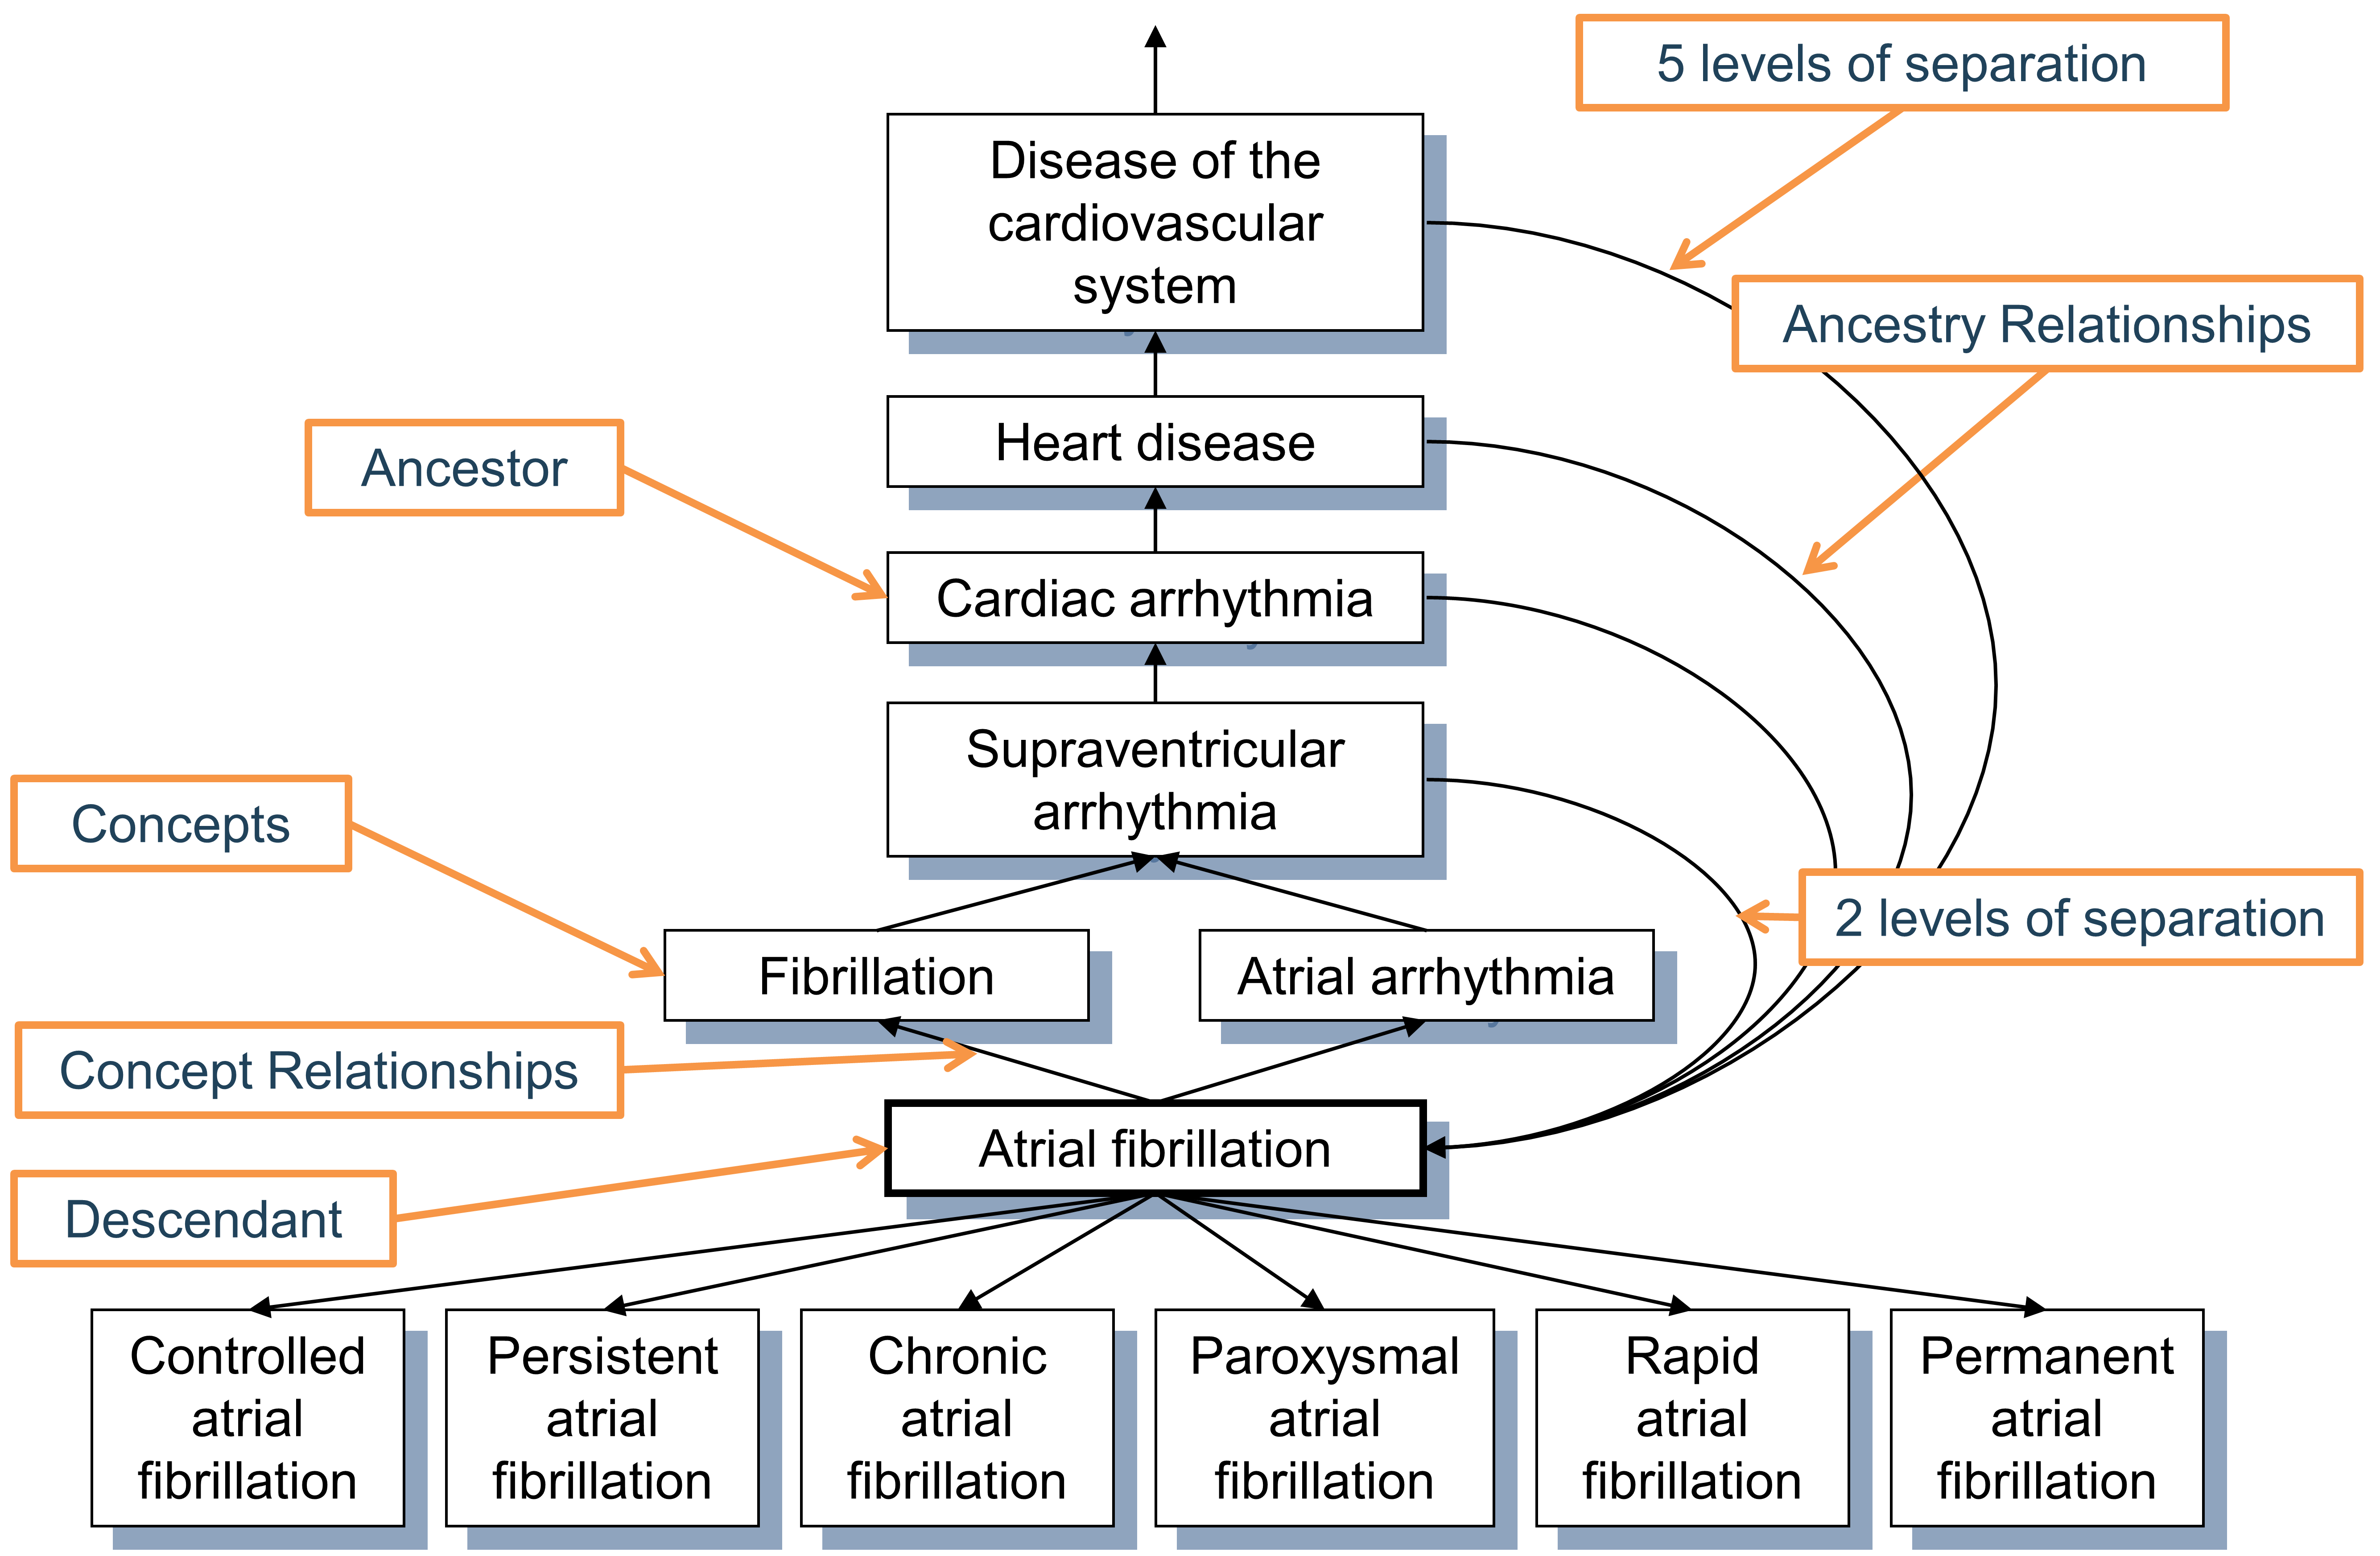
\includegraphics[width=1\linewidth]{images/StandardizedVocabularies/conceptAncestor} 

}

\caption{Hiérarchie de la condition ``Fibrillation auriculaire.'' La parenté de premier degré est définie par les relations ``Est un'' et ``Subsume'', tandis que toutes les relations de degré supérieur sont déduites et stockées dans la table CONCEPT\_ANCESTOR. Chaque concept est également son propre descendant avec les deux niveaux de séparation égaux à 0. \index{concept!ancêtre}}\label{fig:conceptAncestor}
\end{figure}

Le degré d'ascendance, ou le nombre d'étapes entre l'ancêtre et le descendant, est capturé dans les champs MIN\_LEVELS\_OF\_SEPARATION et MAX\_LEVELS\_OF\_SEPARATION, définissant la connexion la plus courte ou la plus longue possible. Toutes les relations hiérarchiques ne contribuent pas de manière égale au calcul des niveaux de séparation. Une étape comptée pour le degré est déterminée par le drapeau IS\_HIERARCHICAL dans la table de référence RELATIONSHIP pour chaque ID de relation.

Actuellement, une hiérarchie complète et de haute qualité n'existe que pour deux domaines : médicament et condition. Les domaines de procédure, mesure et observation ne sont que partiellement couverts et en cours de construction. L'ascendance est particulièrement utile pour le domaine des médicaments car elle permet de parcourir tous les médicaments avec un ingrédient donné ou membres de classes médicamenteuses indépendamment du pays d'origine, du nom de marque ou d'autres attributs.

\section{Tables de Référence Interne}\label{tables-de-ruxe9fuxe9rence-interne}

DOMAIN\_ID, VOCABULARY\_ID, CONCEPT\_CLASS\_ID (tous dans les enregistrements CONCEPT) et CONCEPT\_RELATIONSHIP\_ID (dans CONCEPT\_RELATIONSHIP) sont tous contrôlés par leurs propres vocabulaires. Ils sont définis dans les quatre tables de référence DOMAIN, VOCABULARY, CONCEPT\_CLASS et RELATIONSHIP, contenant les champs *\_ID en tant que clés primaires, un champ *\_NAME plus détaillé et un champ *\_CONCEPT\_ID avec une référence à la table CONCEPT, qui contient un concept pour chaque enregistrement des tables de référence. Le but de ces enregistrements en double est de soutenir un modèle d'information permettant des moteurs de navigation automatiques.

La table VOCABULARY contient également les champs VOCABULARY\_REFERENCE et VOCABULARY\_VERSION se référant à la source et à la version du vocabulaire original. La table RELATIONSHIP comprend les champs supplémentaires DEFINES\_ANCESTRY, IS\_HIERARCHICAL et REVERSE\_RELATIONSHIP\_ID. Ce dernier définit l'ID de relation contrepartie pour une paire de relations.

\section{Situations Spéciales}\label{specialSituations}

\subsection{Genre}\label{genre}

Le genre dans le CDM OMOP et les Vocabularies Standardisés désigne le sexe biologique à la naissance. Souvent, des questions sont posées sur comment définir des genres alternatifs. Ces cas d'utilisation doivent être couverts par des enregistrements dans la table OBSERVATION, où le genre autodéclaré d'une personne est stocké (si l'ensemble de données contient de telles informations).

\subsection{Race et Ethnicité}\label{race-et-ethnicituxe9}

Ces termes suivent les définitions de la façon dont le gouvernement américain les définit. L'ethnicité est une différenciation des populations hispaniques ou non hispaniques, qui peuvent être de n'importe quelle race. La race est divisée en 5 principales races, qui ont des ethnicités comme descendants hiérarchiques. Les races mixtes ne sont pas incluses.

\subsection{Schémas de Codage Diagnostique et Conditions OMOP}\label{schuxe9mas-de-codage-diagnostique-et-conditions-omop}

Les schémas de codage couramment utilisés, tels que l'ICD-9 ou l'ICD-10, définissent des diagnostics plus ou moins bien définis basés sur une démarche diagnostique appropriée. Le domaine des conditions n'est pas identique à cet espace sémantique, mais en partie se chevauche. Par exemple, les conditions incluent également des signes et symptômes enregistrés avant qu'un diagnostic soit établi, et les codes ICD contiennent des concepts appartenant à d'autres domaines (par exemple, les procédures).

\subsection{Systèmes de Codage de Procédures}\label{systuxe8mes-de-codage-de-procuxe9dures}

De même, les schémas de codage comme HCPCS et CPT4 sont censés être des listes de procédures médicales. En réalité, ils sont plus comme un menu de justifications pour le paiement des services médicaux. Bon nombre de ces services sont regroupés sous le domaine des procédures, mais de nombreux concepts échappent à ce domaine.

\subsection{Dispositifs}\label{dispositifs}

Les concepts de dispositifs n'ont pas de schéma de codage standardisé pouvant être utilisé pour sourcer les Concepts Standard. Dans de nombreuses données sources, les dispositifs ne sont même pas codés ou contenus dans un schéma de codage externe. Pour cette même raison, il n'y a actuellement pas de système hiérarchique disponible.

\subsection{Visites et Services}\label{visites-et-services}

Les concepts de visites définissent la nature des rencontres de soins de santé. Dans de nombreux systèmes sources, ils sont appelés Lieu de Service, désignant une organisation ou une structure physique, telle qu'un hôpital. Dans d'autres, ils sont appelés services. Ceux-ci diffèrent également selon les pays, et leur définition est difficile à obtenir. Les sites de soins se spécialisent souvent dans une ou quelques visites (Hôpital XYZ), mais ne doivent pas être définis par elles (même à l'hôpital XYZ, les patients peuvent rencontrer des visites non hospitalières).

\subsection{Fournisseurs et Spécialités}\label{fournisseurs-et-spuxe9cialituxe9s}

Tout fournisseur humain est défini dans le domaine des fournisseurs. Ceux-ci peuvent être des professionnels de santé tels que des médecins et infirmiers, mais aussi des fournisseurs non médicaux comme des optométristes ou des cordonniers. Les spécialités sont des descendants du fournisseur ``Médecin.'' Les sites de soins ne peuvent pas porter une spécialité, même s'ils sont souvent définis par la spécialité de leur personnel principal (``Département de Chirurgie'').

\subsection{Domaines Thérapeutiques aux Besoins Spéciaux}\label{domaines-thuxe9rapeutiques-aux-besoins-spuxe9ciaux}

Les Vocabulaires Standardisés couvrent tous les aspects des soins de santé de manière exhaustive. Cependant, certains domaines thérapeutiques ont des besoins particuliers et nécessitent des vocabulaires spécifiques. Des exemples incluent l'oncologie, la radiologie et la génomique. Des Groupes de Travail OHDSI spécials développent ces extensions. En conséquence, les Vocabulaires Standardisés OMOP constituent un système intégré, où les concepts de différentes origines et objectifs résident tous dans les mêmes hiérarchies spécifiques aux domaines.

\subsection{Concepts Standards dans le Domaine des Médicaments}\label{rxNormExtension}

De nombreux concepts du domaine des médicaments sont issus de RxNorm, un vocabulaire disponible publiquement produit par la US National Library of Medicine. Cependant, les médicaments en dehors des États-Unis peuvent ou non être couverts, en fonction de la commercialisation ou non de la combinaison ingrédient, forme et concentration aux États-Unis. Les médicaments qui ne sont pas sur le marché américain sont ajoutés par l'équipe de vocabulaire OHDSI sous un vocabulaire appelé \href{https://www.ohdsi.org/web/wiki/doku.php?id=documentation:vocabulary:rxnorm_extension}{RxNorm Extension}, qui est le seul grand vocabulaire de domaine produit par OHDSI.

\subsection{Variantes de NULL}\label{variantes-de-null}

De nombreux vocabulaires contiennent des codes concernant l'absence d'information. Par exemple, parmi les cinq concepts de genre 8507 ``Homme,'' 8532 ``Femme,'' 8570 ``Ambigu,'' 8551 ``Inconnu,'' et 8521 ``Autre'', seuls les deux premiers sont Standards, et les trois autres sont des concepts sources sans mappage. Dans les Vocabulaires Standardisés, il n'y a aucune distinction faite sur la raison pour laquelle une information est indisponible ; cela peut être dû à un retrait actif de l'information par le patient, une valeur manquante, une valeur non définie ou standardisée de quelque manière que ce soit, ou l'absence d'un enregistrement de mappage dans CONCEPT\_RELATIONSHIP. Tout concept ainsi désigné n'est pas mappé, ce qui correspond à un mappage par défaut vers le Concept Standard avec l'ID de concept = 0.

\section{Résumé}\label{ruxe9sumuxe9-3}

\begin{rmdsummary}
\begin{itemize}
\tightlist
\item
  Tous les événements et les faits administratifs sont représentés dans les Vocabulaires Standardisés OMOP comme des concepts, des relations de concepts, et une hiérarchie d'ancêtres de concepts.
\item
  La plupart de ceux-ci sont adoptés à partir de schémas de codage ou de vocabulaires existants, bien que certains d'entre eux soient créés de novo par l'équipe de vocabulaire OHDSI.
\item
  Tous les concepts se voient attribuer un domaine, lequel contrôle où le fait représenté par le concept est stocké dans le CDM.
\item
  Les concepts de signification équivalente dans différents vocabulaires sont mappés à l'un d'eux, lequel est désigné comme le Concept Standard. Les autres sont des concepts sources.
\item
  Le mappage est effectué par les relations de concepts ``Maps to'' et ``Maps to value''.
\item
  Il existe une classe supplémentaire de concepts appelés concepts de classification, qui ne sont pas standards, mais contrairement aux concepts sources, ils participent à la hiérarchie.
\item
  Les concepts ont un cycle de vie dans le temps.
\item
  Les concepts au sein d'un domaine sont organisés en hiérarchies. La qualité de la hiérarchie diffère entre les domaines, et l'achèvement du système hiérarchique est une tâche en cours.
\item
  Vous êtes vivement encouragé à contacter la communauté si vous pensez avoir trouvé une erreur ou une inexactitude.
\end{itemize}
\end{rmdsummary}

\section{Exercices}\label{exercices-1}

\subsubsection*{Prérequis}\label{pruxe9requis-2}
\addcontentsline{toc}{subsubsection}{Prérequis}

Pour ces premiers exercices, vous devrez rechercher des concepts dans les Vocabulaires Standardisés, ce qui peut être fait via ATHENA\footnote{\url{http://athena.ohdsi.org/}} ou ATLAS.\footnote{\url{http://atlas-demo.ohdsi.org}}

\begin{exercise}
\protect\hypertarget{exr:exerciseVocab1}{}\label{exr:exerciseVocab1}Quel est l'ID de Concept Standard pour ``Hémorragie gastro-intestinale'' ?
\end{exercise}

\begin{exercise}
\protect\hypertarget{exr:exerciseVocab2}{}\label{exr:exerciseVocab2}Quels codes ICD-10CM sont mappés au Concept Standard pour ``Hémorragie gastro-intestinale'' ? Quels codes ICD-9CM sont mappés à ce Concept Standard ?
\end{exercise}

\begin{exercise}
\protect\hypertarget{exr:exerciseVocab3}{}\label{exr:exerciseVocab3}Quels sont les termes préférés MedDRA équivalents au Concept Standard pour ``Hémorragie gastro-intestinale'' ?
\end{exercise}

Les réponses suggérées peuvent être trouvées en Annexe \ref{Vocabanswers}.

\chapter{Extraction, Transformation et Chargement}\label{ExtractTransformLoad}

\emph{Responsables de chapitre : Clair Blacketer \& Erica Voss}

\section{Introduction}\label{introduction-1}

Pour convertir les données natives/brutes au Modèle de Données Commun OMOP (CDM), nous devons créer un processus d'extraction, transformation et chargement (ETL). Ce processus doit restructurer les données selon le CDM, ajouter des correspondances aux Vocabularies Standardisés, et il est généralement implémenté sous forme de scripts automatisés, par exemple des scripts SQL. Il est important que ce processus ETL soit répétable, afin qu'il puisse être relancé à chaque fois que les données sources sont actualisées. \index{ETL|see {extraction, transformation et chargement (ETL)}} \index{données brutes} \index{données natives|see {données brutes}} \index{données sources|see{données brutes}}

La création d'un ETL est généralement une entreprise de grande envergure. Au fil des années, nous avons développé des meilleures pratiques, consistant en quatre étapes principales :

\begin{enumerate}
\def\labelenumi{\arabic{enumi}.}
\tightlist
\item
  Des experts en données et des experts en CDM conçoivent ensemble l'ETL.
\item
  Des personnes ayant des connaissances médicales créent les correspondances de code.
\item
  Une personne technique met en œuvre l'ETL.
\item
  Tous sont impliqués dans le contrôle de qualité.
\end{enumerate}

Dans ce chapitre, nous discuterons en détail de chacune de ces étapes. Plusieurs outils ont été développés par la communauté OHDSI pour soutenir certaines de ces étapes, et ceux-ci seront également abordés. Nous terminerons ce chapitre par une discussion sur la maintenance du CDM et de l'ETL.
\#\# Étape 1 : Concevoir l'ETL

Il est important de bien distinguer la conception de l'ETL de sa mise en œuvre. La conception de l'ETL nécessite une connaissance approfondie à la fois des données sources et du CDM. La mise en œuvre de l'ETL, en revanche, repose principalement sur une expertise technique pour rendre l'ETL efficace en termes de calcul. Si nous essayons de faire les deux en même temps, nous risquons de nous enliser dans des détails insignifiants, alors que nous devrions nous concentrer sur l'ensemble du tableau.

Deux outils étroitement intégrés ont été développés pour soutenir le processus de conception de l'ETL : White Rabbit et Rabbit-in-a-Hat.

\subsection{White Rabbit}\label{white-rabbit}

Pour initier un processus ETL sur une base de données, vous devez comprendre vos données, y compris les tables, les champs et le contenu. C'est là que l'outil \href{https://github.com/OHDSI/WhiteRabbit}{White Rabbit} entre en jeu. White Rabbit est un logiciel destiné à aider à préparer les ETL des bases de données longitudinales de soins de santé pour les transformer en \href{https://github.com/OHDSI/CommonDataModel}{OMOP CDM}. White Rabbit scanne vos données et crée un rapport contenant toutes les informations nécessaires pour commencer à concevoir l'ETL. Tout le code source et les instructions d'installation, ainsi qu'un lien vers le manuel, sont disponibles sur GitHub.\footnote{\url{https://github.com/OHDSI/WhiteRabbit}.} \index{White Rabbit} \index{profilage de données|see {White Rabbit}}

\subsubsection*{Portée et objectif}\label{portuxe9e-et-objectif}
\addcontentsline{toc}{subsubsection}{Portée et objectif}

La fonction principale de White Rabbit est d'effectuer un scan des données sources, fournissant des informations détaillées sur les tables, les champs et les valeurs présentes dans un champ. Les données sources peuvent être dans des fichiers texte séparés par des virgules, ou dans une base de données (MySQL, SQL Server, Oracle, PostgreSQL, Microsoft APS, Microsoft Access, Amazon Redshift). Le scan générera un rapport utilisable comme référence lors de la conception de l'ETL, par exemple en l'utilisant conjointement avec l'outil Rabbit-In-a-Hat. White Rabbit se distingue des outils de profilage de données standard en tentant d'empêcher l'affichage de données personnellement identifiables (PII) dans le fichier de sortie généré.

\subsubsection*{Vue d'ensemble du processus}\label{vue-densemble-du-processus}
\addcontentsline{toc}{subsubsection}{Vue d'ensemble du processus}

La séquence typique pour utiliser le logiciel afin de scanner les données sources :

\begin{enumerate}
\def\labelenumi{\arabic{enumi}.}
\tightlist
\item
  Définir le dossier de travail, l'emplacement sur l'ordinateur de bureau local où les résultats seront exportés.
\item
  Connecter à la base de données source ou au fichier texte CSV et tester la connexion.
\item
  Sélectionner les tables d'intérêt pour le scan et scanner les tables.
\item
  White Rabbit crée une exportation des informations sur les données sources.
\end{enumerate}

\subsubsection*{Définir un dossier de travail}\label{duxe9finir-un-dossier-de-travail}
\addcontentsline{toc}{subsubsection}{Définir un dossier de travail}

Après avoir téléchargé et installé l'application White Rabbit, la première chose à faire est de définir un dossier de travail. Tous les fichiers créés par White Rabbit seront exportés dans ce dossier local. Utilisez le bouton ``Pick Folder'' illustré à la Figure \ref{fig:WhiteRabbitLocation} pour naviguer dans votre environnement local là où vous souhaitez que le document de scan soit enregistré.

\begin{figure}

{\centering 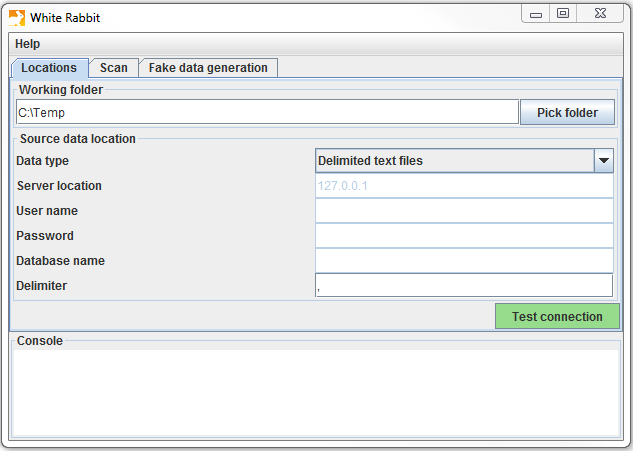
\includegraphics[width=1\linewidth]{images/ExtractTransformLoad/WhiteRabbitLocation} 

}

\caption{Le bouton "Pick Folder" permet de spécifier un dossier de travail pour l'application White Rabbit.}\label{fig:WhiteRabbitLocation}
\end{figure}

\subsubsection*{Connexion à une base de données}\label{connexion-uxe0-une-base-de-donnuxe9es}
\addcontentsline{toc}{subsubsection}{Connexion à une base de données}

White Rabbit prend en charge les fichiers texte délimités et diverses plates-formes de base de données. Survolez les différents champs avec la souris pour obtenir une description de ce qui est requis. Des informations plus détaillées se trouvent dans le manuel.

\subsubsection*{Scanner les tables dans une base de données}\label{scanner-les-tables-dans-une-base-de-donnuxe9es}
\addcontentsline{toc}{subsubsection}{Scanner les tables dans une base de données}

Après connexion à une base de données, vous pouvez scanner les tables qu'elle contient. Un scan génère un rapport contenant des informations sur les données sources utilisables pour aider à concevoir l'ETL. En utilisant l'onglet Scan illustré à la Figure \ref{fig:WhiteRabbitAddTables}, vous pouvez soit sélectionner des tables individuelles dans la base de données source sélectionnée en cliquant sur ``Add'' (Ctrl + clic de souris), ou sélectionner automatiquement toutes les tables de la base de données en cliquant sur ``Add all in DB''.

\begin{figure}

{\centering 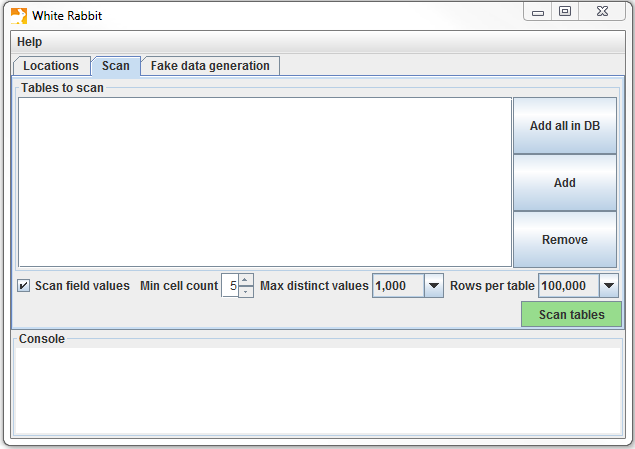
\includegraphics[width=1\linewidth]{images/ExtractTransformLoad/WhiteRabbitAddTables} 

}

\caption{Onglet de scan de White Rabbit.}\label{fig:WhiteRabbitAddTables}
\end{figure}

Il y a également quelques options de paramétrage avec le scan :

\begin{itemize}
\tightlist
\item
  Cocher ``Scan field values'' indique à White Rabbit que vous souhaitez examiner les valeurs apparaissant dans les colonnes.
\item
  ``Min cell count'' est une option lors du scan des valeurs de champ. Par défaut, elle est définie à 5, ce qui signifie que les valeurs des données sources apparaissant moins de 5 fois n'apparaîtront pas dans le rapport. Les ensembles de données individuels peuvent avoir leurs propres règles concernant ce nombre minimal de cellules.
\item
  ``Rows per table'' est une option lors du scan des valeurs de champ. Par défaut, White Rabbit scannera 100,000 lignes sélectionnées au hasard dans la table.
\end{itemize}

Une fois tous les paramètres complétés, appuyez sur le bouton ``Scan tables''. Après la fin du scan, le rapport sera écrit dans le dossier de travail.

\subsubsection*{Interpréter le rapport de scan}\label{interpruxe9ter-le-rapport-de-scan}
\addcontentsline{toc}{subsubsection}{Interpréter le rapport de scan}

Une fois le scan terminé, un fichier Excel est généré dans le dossier sélectionné, avec un onglet pour chaque table scannée ainsi qu'un onglet récapitulatif. L'onglet récapitulatif liste toutes les tables scannées, chaque champ dans chaque table, le type de données de chaque champ, la longueur maximale du champ, le nombre de lignes dans la table, le nombre de lignes scannées, et la fréquence à laquelle chaque champ a été trouvé vide. La Figure \ref{fig:ScanOverviewTab}. montre un exemple d'onglet récapitulatif.

\begin{figure}

{\centering 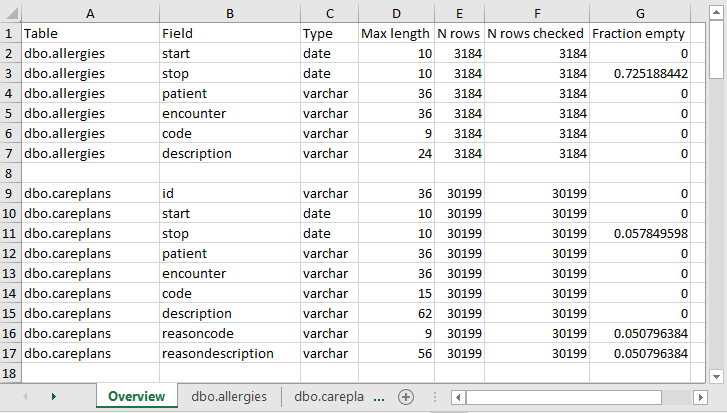
\includegraphics[width=1\linewidth]{images/ExtractTransformLoad/ScanOverviewTab} 

}

\caption{Exemple d'onglet récapitulatif d'un rapport de scan.}\label{fig:ScanOverviewTab}
\end{figure}

Les onglets pour chaque table montrent chaque champ, les valeurs dans chaque champ et la fréquence de chaque valeur. Chaque colonne de la table source générera deux colonnes dans le fichier Excel. Une colonne listera toutes les valeurs distinctes ayant un nombre supérieur au ``Min cell count'' défini au moment du scan. Si une liste de valeurs uniques était tronquée, la dernière valeur dans la liste sera ``List truncated''; cela indique qu'il y a une ou plusieurs valeurs uniques additionnelles apparaissant moins souvent que le nombre saisi dans le ``Min cell count''. À côté de chaque valeur distincte se trouve une deuxième colonne contenant la fréquence (le nombre de fois que cette valeur apparaît dans l'échantillon). Ces deux colonnes (valeurs distinctes et fréquence) se répètent pour toutes les colonnes sources de la table profilée dans le classeur.

\begin{figure}

{\centering 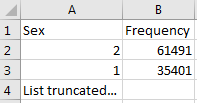
\includegraphics[width=0.3\linewidth]{images/ExtractTransformLoad/ScanSex} 

}

\caption{Exemple de valeurs pour une seule colonne.}\label{fig:scanSex}
\end{figure}

Le rapport est puissant pour comprendre vos données sources en mettant en évidence ce qui existe. Par exemple, si les résultats illustrés à la Figure \ref{fig:scanSex} étaient retournés pour la colonne ``Sex'' dans une des tables scannées, nous pouvons voir qu'il y avait deux valeurs communes (1 et 2) apparaissant 61,491 et 35,401 fois respectivement. White Rabbit ne définira pas 1 comme masculin et 2 comme féminin; le détenteur des données devront généralement définir les codes sources uniques au système source. Cependant, ces deux valeurs (1 \& 2) ne sont pas les seules présentes dans les données car nous voyons que cette liste a été tronquée. Ces autres valeurs apparaissent très peu fréquemment (défini par le ``Min cell count'') et représentent souvent des valeurs incorrectes ou très suspectes. Lors de la génération d'un ETL, nous devons non seulement planifier pour les concepts de genre haute fréquence 1 et 2 mais aussi pour les autres valeurs basse fréquence existant dans cette colonne. Par exemple, si ces genres basse fréquence étaient ``NULL'', nous devons nous assurer que l'ETL peut traiter ces données et sait quoi faire dans cette situation.

\subsection{Rabbit-In-a-Hat}\label{rabbit-in-a-hat}

Avec le scan de White Rabbit en main, nous avons une image claire des données sources. Nous connaissons également la spécification complète du CDM. Maintenant, nous devons définir la logique pour passer de l'un à l'autre. Cette activité de conception nécessite une connaissance approfondie à la fois des données sources et du CDM. Les outils Rabbit-in-a-Hat qui accompagnent le logiciel White Rabbit sont spécialement conçus pour soutenir une équipe d'experts dans ces domaines. Dans un cadre typique, l'équipe de conception de l'ETL se réunit dans une salle, tandis que Rabbit-in-a-Hat est projeté sur un écran. Lors d'un premier tour, les mappages tables-à-tables peuvent être décidés collaborativement, après quoi les mappages de champ-à-champ peuvent être conçus, tout en définissant la logique par laquelle les valeurs seront transformées. \index{Rabbit-In-A-Hat} \index{conception d'ETL|see {Rabbit-In-A-Hat}}

\subsubsection*{Portée et objectif}\label{portuxe9e-et-objectif-1}
\addcontentsline{toc}{subsubsection}{Portée et objectif}

Rabbit-In-a-Hat est conçu pour lire et afficher un document de scan de White Rabbit. White Rabbit génère des informations sur les données sources tandis que Rabbit-In-a-Hat utilise ces informations et grâce à une interface graphique permet à un utilisateur de connecter les données sources aux tables et colonnes du CDM. Rabbit-In-a-Hat génère de la documentation pour le processus ETL, il ne génère pas de code pour créer un ETL.

\subsubsection*{Vue d'ensemble du processus}\label{vue-densemble-du-processus-1}
\addcontentsline{toc}{subsubsection}{Vue d'ensemble du processus}

La séquence typique pour utiliser ce logiciel afin de générer la documentation d'un ETL :

\begin{enumerate}
\def\labelenumi{\arabic{enumi}.}
\tightlist
\item
  Résultats scannés de WhiteRabbit terminés.
\item
  Ouvrir les résultats scannés; l'interface affiche les tables sources et les tables CDM.
\item
  Connecter les tables sources aux tables CDM où la table source fournit des informations pour cette table CDM correspondante.
\item
  Pour chaque connexion table source à table CDM, définir davantage la connexion avec les détails colonne source à colonne CDM.
\item
  Enregistrer le travail de Rabbit-In-a-Hat et l'exporter vers un document MS Word.
\end{enumerate}

\subsubsection*{Rédaction de la logique ETL}\label{ruxe9daction-de-la-logique-etl}
\addcontentsline{toc}{subsubsection}{Rédaction de la logique ETL}

Une fois que vous avez ouvert votre rapport de scan White Rabbit dans Rabbit-In-a-Hat, vous êtes prêt à commencer à concevoir et à rédiger la logique pour convertir les données sources en OMOP CDM. À titre d'exemple, les sections suivantes illustreront comment certaines des tables de la base de données Synthea\footnote{Synthea\textsuperscript{TM} est un générateur de patients visant à modéliser de vrais patients. Les données sont créées en fonction des paramètres passés à l'application. La structure des données se trouve ici : \url{https://github.com/synthetichealth/synthea/wiki}.} pourraient apparaître lors de la conversion.

\subsubsection*{Flux général d'un ETL}\label{flux-guxe9nuxe9ral-dun-etl}
\addcontentsline{toc}{subsubsection}{Flux général d'un ETL}

Étant donné que le CDM est un modèle centré sur la personne, il est toujours judicieux de commencer par mapper la table PERSON. Chaque table d'événement clinique (CONDITION\_OCCURRENCE, DRUG\_EXPOSURE, PROCEDURE\_OCCURRENCE, etc.) se réfère à la table PERSON via le person\_id ; élaborer la logique pour la table PERSON en premier rend la tâche plus facile par la suite. Après la table PERSON, une bonne règle de base est de convertir la table OBSERVATION\_PERIOD ensuite. Chaque personne dans une base de données CDM doit avoir au moins une OBSERVATION\_PERIOD et, en général, la plupart des événements pour une personne se produisent dans ce laps de temps. Une fois les tables PERSON et OBSERVATION\_PERIOD terminées, les tables dimensionnelles comme PROVIDER, CARE\_SITE et LOCATION sont généralement les suivantes. La logique des tables finale à travailler avant les tables cliniques est VISIT\_OCCURRENCE. Cela est souvent la logique la plus compliquée dans tout l'ETL et elle est parmi les plus cruciales car la plupart des événements se produisant au cours du parcours du patient se produiront pendant les visites. Une fois ces tables terminées, il est de votre choix de mapper les tables CDM et dans l'ordre que vous préférez.

\begin{figure}

{\centering 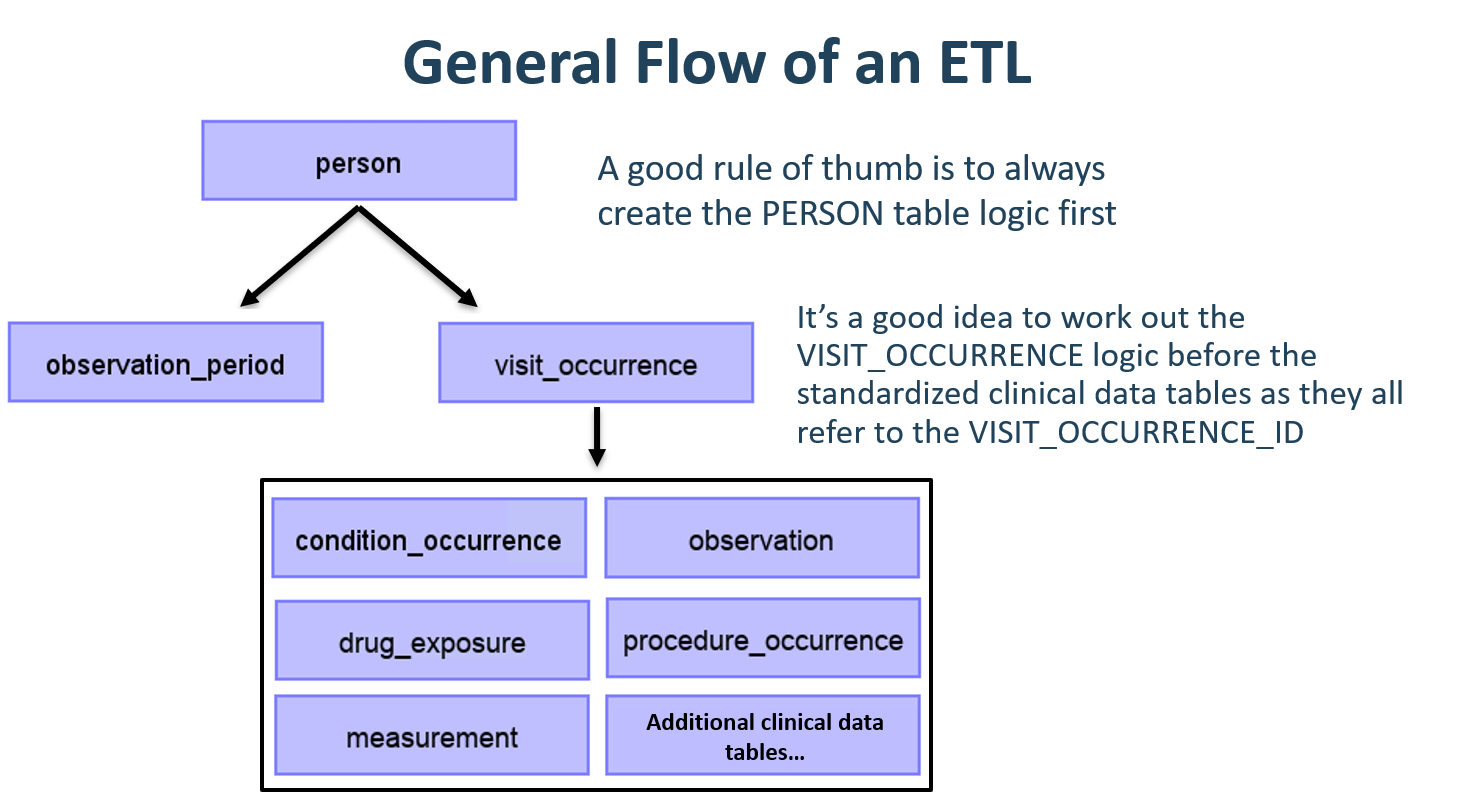
\includegraphics[width=1\linewidth]{images/ExtractTransformLoad/flowOfEtl} 

}

\caption{Flux général d'un ETL et quelles tables mapper en premier.}\label{fig:etlFlow}
\end{figure}

Il est souvent nécessaire, lors de la conversion au CDM, de prévoir des tables intermédiaires. Cela pourrait être pour attribuer les bons VISIT\_OCCURRENCE\_IDs aux événements, ou pour mapper les codes sources aux concepts standard (faire cette étape dynamique est souvent très lent). Les tables intermédiaires sont 100 \% autorisées et encouragées. Ce qui est découragé, c'est la persistance et la dépendance à l'égard de ces tables intermédiaires une fois la conversion terminée.

\subsubsection*{Exemple de mappage : Table Person}\label{exemple-de-mappage-table-person}
\addcontentsline{toc}{subsubsection}{Exemple de mappage : Table Person}

La structure des données Synthea contient 20 colonnes dans la table patients, mais toutes n'étaient pas nécessaires pour peupler la table PERSON, comme illustré à la Figure \ref{fig:syntheaPerson}. Cela est très courant et ne devrait pas être alarmant. Dans cet exemple, de nombreux points de données de la table patients de Synthea qui n'ont pas été utilisés dans la table PERSON du CDM étaient des identifiants supplémentaires tels que le nom du patient, le numéro de permis de conduire et le numéro de passeport.

\begin{figure}

{\centering 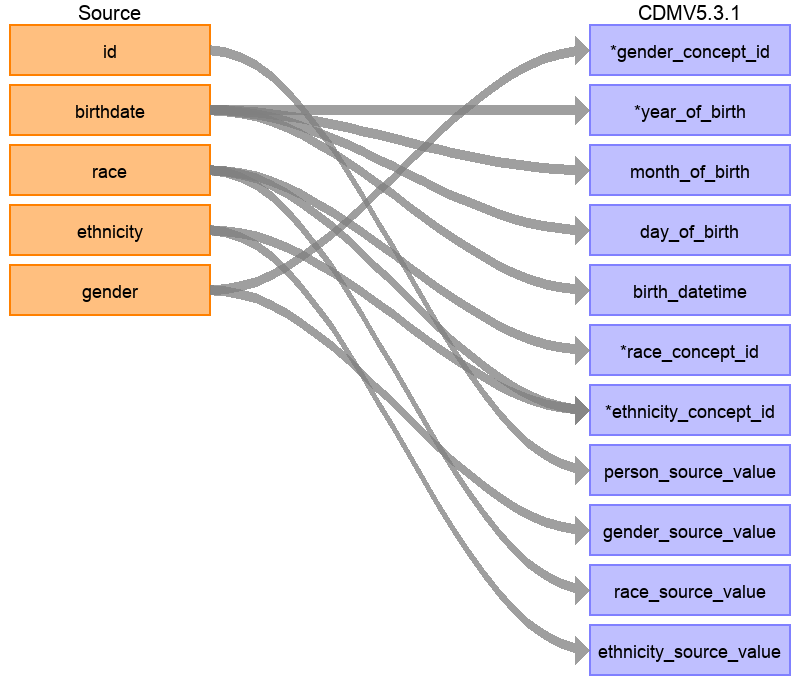
\includegraphics[width=1\linewidth]{images/ExtractTransformLoad/syntheaPersonTable} 

}

\caption{Mise en correspondance de la table Patients de Synthea avec la table PERSON du CDM.}\label{fig:syntheaPerson}
\end{figure}

Le tableau \ref{tab:syntheaEtlPerson} ci-dessous montre la logique qui a été imposée à la table patients de Synthea pour la convertir en table PERSON du CDM. La colonne `Destination Field' discute où dans le CDM les données sont mappées. La colonne `Source field' met en évidence la colonne de la table source (dans ce cas patients) qui sera utilisée pour peupler la colonne CDM. Enfin, la colonne `Logic \& comments' donne des explications pour la logique.

Table : \label{tab:syntheaEtlPerson} Logique ETL pour convertir la table Patients de Synthea en table PERSON du CDM.

\begin{longtable}[]{@{}
  >{\raggedright\arraybackslash}p{(\columnwidth - 4\tabcolsep) * \real{0.3108}}
  >{\raggedright\arraybackslash}p{(\columnwidth - 4\tabcolsep) * \real{0.1351}}
  >{\raggedright\arraybackslash}p{(\columnwidth - 4\tabcolsep) * \real{0.5541}}@{}}
\toprule\noalign{}
\begin{minipage}[b]{\linewidth}\raggedright
Destination Field
\end{minipage} & \begin{minipage}[b]{\linewidth}\raggedright
Source field
\end{minipage} & \begin{minipage}[b]{\linewidth}\raggedright
Logic \& comments
\end{minipage} \\
\midrule\noalign{}
\endhead
\bottomrule\noalign{}
\endlastfoot
PERSON\_ID & & Généré automatiquement. Le PERSON\_ID sera généré au moment de l'implémentation. Cela est dû au fait que la valeur de l'identifiant source est une valeur varchar tandis que le PERSON\_ID est un entier. Le champ id de la source est défini comme PERSON\_SOURCE\_VALUE pour préserver cette valeur et permettre la vérification des erreurs si nécessaire. \\
GENDER\_CONCEPT\_ID & gender & Lorsque gender = `M', définir GENDER\_CONCEPT\_ID à 8507, lorsque gender = `F', définir à 8532. Supprimer toutes les lignes avec un sexe manquant/inconnu. Ces deux concepts ont été choisis car ce sont les seuls concepts standard dans le domaine du sexe. Le choix de supprimer les patients avec des sexes inconnus tend à être basé sur le site, bien qu'il soit recommandé de les supprimer car les personnes sans sexe sont exclues des analyses. \\
YEAR\_OF\_BIRTH & birthdate & Extraire l'année de la date de naissance \\
MONTH\_OF\_BIRTH & birthdate & Extraire le mois de la date de naissance \\
DAY\_OF\_BIRTH & birthdate & Extraire le jour de la date de naissance \\
BIRTH\_DATETIME & birthdate & À minuit, heure 00:00:00. Ici, la source n'a pas fourni d'heure de naissance, donc l'option choisie a été de la fixer à minuit. \\
RACE\_CONCEPT\_ID & race & Lorsque race = `WHITE', définir à 8527, lorsque race = `BLACK', définir à 8516, lorsque race = `ASIAN', définir à 8515, sinon définir à 0. Ces concepts ont été choisis car ce sont des concepts standard appartenant au domaine de la race qui correspondent le plus étroitement aux catégories raciales dans la source. \\
ETHNICITY\_ CONCEPT\_ID & race ethnicity & Lorsque race = `HISPANIC', ou lorsque ethnicity est dans (`CENTRAL\_AMERICAN', `DOMINICAN', `MEXICAN', `PUERTO\_RICAN', `SOUTH\_AMERICAN'), définir à 38003563, sinon définir à 0. Ceci est un bon exemple de la manière dont plusieurs colonnes sources peuvent contribuer à une colonne CDM. Dans le CDM, l'ethnicité est représentée comme soit hispanique soit non hispanique, donc les valeurs des colonnes sources race et ethnicity détermineront cette valeur. \\
LOCATION\_ID & & \\
PROVIDER\_ID & & \\
CARE\_SITE\_ID & & \\
PERSON\_SOURCE\_ VALUE & id & \\
GENDER\_SOURCE\_ VALUE & gender & \\
GENDER\_SOURCE\_ CONCEPT\_ID & & \\
RACE\_SOURCE\_ VALUE & race & \\
RACE\_SOURCE\_ CONCEPT\_ID & & \\
ETHNICITY\_ SOURCE\_VALUE & ethnicity & Dans ce cas, l'ETHNICITY\_SOURCE\_VALUE aura plus de granularité que l'ETHNICITY\_CONCEPT\_ID. \\
ETHNICITY\_ SOURCE\_CONCEPT\_ID & & \\
\end{longtable}

Pour plus d'exemples sur la manière dont l'ensemble de données Synthea a été mappé au CDM, veuillez consulter le document de spécification complète.\footnote{\url{https://ohdsi.github.io/ETL-Synthea/}
  \#\# Étape 2 : Créer les Mappings de Codes}

De plus en plus de codes source sont ajoutés au Vocabulaire OMOP tout le temps. Cela signifie que les systèmes de codage dans les données transformées en CDM peuvent déjà être inclus et mappés. Vérifiez la table VOCABULARY dans le Vocabulaire OMOP pour voir quels vocabulaires sont inclus. Pour extraire le mapping des codes source non standards (par exemple les codes ICD-10CM) vers les concepts standards (par exemple les codes SNOMED), nous pouvons utiliser les enregistrements de la table CONCEPT\_RELATIONSHIP ayant relationship\_id = ``Maps to''. Par exemple, pour trouver l'ID de concept standard pour le code ICD-10CM `I21' (``Infarctus du myocarde aigu''), nous pouvons utiliser la requête SQL suivante :

\begin{Shaded}
\begin{Highlighting}[]
\KeywordTok{SELECT}\NormalTok{ concept\_id\_2 standard\_concept\_id}
\KeywordTok{FROM}\NormalTok{ concept\_relationship}
\KeywordTok{INNER} \KeywordTok{JOIN}\NormalTok{ concept source\_concept}
  \KeywordTok{ON}\NormalTok{ concept\_id }\OperatorTok{=}\NormalTok{ concept\_id\_1}
\KeywordTok{WHERE}\NormalTok{ concept\_code }\OperatorTok{=} \StringTok{\textquotesingle{}I21\textquotesingle{}}
  \KeywordTok{AND}\NormalTok{ vocabulary\_id }\OperatorTok{=} \StringTok{\textquotesingle{}ICD10CM\textquotesingle{}}
  \KeywordTok{AND}\NormalTok{ relationship\_id }\OperatorTok{=} \StringTok{\textquotesingle{}Maps to\textquotesingle{}}\NormalTok{;}
\end{Highlighting}
\end{Shaded}

\begin{longtable}[]{@{}r@{}}
\toprule\noalign{}
STANDARD\_CONCEPT\_ID \\
\midrule\noalign{}
\endhead
\bottomrule\noalign{}
\endlastfoot
312327 \\
\end{longtable}

Malheureusement, parfois, les données source utilisent des systèmes de codage qui ne sont pas dans le Vocabulaire. Dans ce cas, un mapping doit être créé entre le système de codage source et les Concepts Standards. La cartographie de codes peut être une tâche intimidante, surtout lorsqu'il y a de nombreux codes dans le système de codage source. Il y a plusieurs choses qui peuvent être faites pour faciliter cette tâche :

\begin{itemize}
\tightlist
\item
  Concentrez-vous sur les codes les plus fréquemment utilisés. Un code qui n'est jamais ou rarement utilisé ne vaut pas l'effort de la cartographie, puisqu'il ne sera jamais utilisé dans une étude réelle.
\item
  Utilisez les informations existantes chaque fois que possible. Par exemple, de nombreux systèmes nationaux de codage des médicaments ont été mappés à l'ATC. Bien que l'ATC ne soit pas suffisamment détaillé pour de nombreux usages, les relations de concepts entre l'ATC et RxNorm peuvent être utilisées pour faire de bonnes suppositions sur les bons codes RxNorm.
\item
  Utilisez Usagi.
\end{itemize}

\subsection{Usagi}\label{usagi}

Usagi est un outil pour aider au processus manuel de création d'un mapping de codes. Il peut faire des suggestions de mappings basées sur la similarité textuelle des descriptions de codes. Si les codes source ne sont disponibles que dans une langue étrangère, nous avons constaté que Google Translate\footnote{\url{https://translate.google.com/}} fournit souvent une traduction étonnamment bonne des termes en anglais. Usagi permet à l'utilisateur de rechercher les concepts cibles appropriés si la suggestion automatisée n'est pas correcte. Enfin, l'utilisateur peut indiquer quels mappings sont approuvés pour être utilisés dans l'ETL. Usagi est disponible sur GitHub.\footnote{\url{https://github.com/OHDSI/Usagi}} \index{Usagi} \index{cartographie de code source|see {Usagi}}

\subsubsection*{Portée et But}\label{portuxe9e-et-but}
\addcontentsline{toc}{subsubsection}{Portée et But}

Les codes source nécessitant un mapping sont chargés dans Usagi (si les codes ne sont pas en anglais, des colonnes supplémentaires de traductions sont nécessaires). Une approche de similarité de termes est utilisée pour connecter les codes source aux concepts du Vocabulaire. Cependant, ces connexions de codes doivent être revues manuellement et Usagi fournit une interface pour faciliter cela. Usagi ne proposera que des concepts marqués comme Concepts Standards dans le Vocabulaire.

\subsubsection*{Vue d'ensemble du processus}\label{vue-densemble-du-processus-2}
\addcontentsline{toc}{subsubsection}{Vue d'ensemble du processus}

La séquence typique pour utiliser ce logiciel est :

\begin{enumerate}
\def\labelenumi{\arabic{enumi}.}
\tightlist
\item
  Chargez les codes de votre système source (``codes source'') que vous souhaitez mapper aux concepts du Vocabulaire.
\item
  Usagi exécutera une approche de similarité de termes pour mapper les codes source aux concepts du Vocabulaire.
\item
  Utilisez l'interface d'Usagi pour vérifier et, si nécessaire, améliorer les mappings suggérés. De préférence, une personne ayant de l'expérience avec le système de codage et la terminologie médicale doit être utilisée pour cette revue.
\item
  Exportez le mapping vers la table SOURCE\_TO\_CONCEPT\_MAP du Vocabulaire.
\end{enumerate}

\subsubsection*{Importer les Codes Source dans Usagi}\label{importer-les-codes-source-dans-usagi}
\addcontentsline{toc}{subsubsection}{Importer les Codes Source dans Usagi}

Exportez les codes source de votre système source dans un fichier CSV ou Excel (.xlsx). Ce fichier doit contenir au moins des colonnes comprenant le code source et une description du code source en anglais. Cependant, des informations supplémentaires sur les codes peuvent également être incluses (par exemple, unité de dose, ou la description dans la langue d'origine si traduite). En plus des informations sur les codes source, la fréquence du code devrait également être incluse, car cela peut aider à prioriser les codes qui nécessitent le plus d'effort pour le mapping (par exemple, vous pouvez avoir 1 000 codes source, mais seulement 100 sont réellement utilisés dans le système). Si des informations sur les codes source doivent être traduites en anglais, utilisez Google Translate.

Note : les extractions de codes source doivent être divisées par domaine (c'est-à-dire médicaments, procédures, conditions, observations) et non regroupées dans un fichier volumineux.

Les codes source sont chargés dans Usagi depuis le menu File --\textgreater{} Import codes. De là, un ``Import codes \ldots{}'' s'affichera comme montré dans la Figure \ref{fig:usagiImport}. Dans cette figure, les termes des codes source étaient en néerlandais et ont également été traduits en anglais. Usagi utilisera les traductions anglaises pour mapper au vocabulaire standard.

\begin{figure}

{\centering 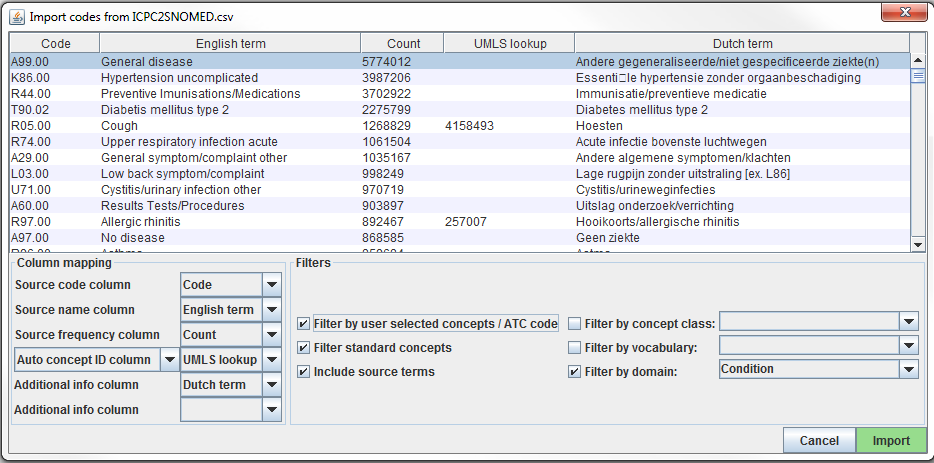
\includegraphics[width=1\linewidth]{images/ExtractTransformLoad/usagiImport} 

}

\caption{Usagi source code input screen.}\label{fig:usagiImport}
\end{figure}

La section ``Column mapping'' (en bas à gauche) est l'endroit où vous définissez pour Usagi comment utiliser la table importée. Si vous passez la souris sur les menus déroulants, une fenêtre contextuelle apparaîtra définissant chaque colonne. Usagi n'utilisera pas la ou les colonnes ``Additional info'' comme informations pour associer les codes source aux codes de concept du Vocabulaire ; cependant, ces informations supplémentaires peuvent aider la personne qui révise le mapping des codes source et devraient être incluses.

Enfin, dans la section ``Filters'' (en bas à droite), vous pouvez définir certaines restrictions pour Usagi lors du mapping. Par exemple, dans la Figure \ref{fig:usagiImport}, l'utilisateur mappe les codes source uniquement aux concepts du domaine Condition. Par défaut, Usagi ne mappe que vers les Concepts Standards, mais si l'option ``Filter standard concepts'' est désactivée, Usagi considérera également les Concepts de Classification. Passez la souris sur les différents filtres pour plus d'informations sur le filtre.

Un filtre spécial est ``Filter by automatically selected concepts / ATC code''. Si vous disposez de certaines informations que vous pouvez utiliser pour restreindre la recherche, vous pouvez le faire en fournissant une liste de CONCEPT\_ID ou un code ATC dans la colonne indiquée dans la colonne Auto concept ID (délimitée par un point-virgule). Par exemple, dans le cas des médicaments, il se peut que des codes ATC soient déjà assignés à chaque médicament. Même si un code ATC n'identifie pas de manière unique un seul code de médicament RxNorm, il aide à limiter l'espace de recherche à seulement ces concepts qui relèvent du code ATC dans le Vocabulaire. Pour utiliser le code ATC, suivez ces étapes :

\begin{enumerate}
\def\labelenumi{\arabic{enumi}.}
\tightlist
\item
  Dans la section Column mapping, passez de ``Auto concept ID column'' à ``ATC column''.
\item
  Dans la section Column mapping, sélectionnez la colonne contenant le code ATC comme ``ATC column''.
\item
  Activez ``Filter by user selected concepts / ATC code'' dans la section Filters.
\end{enumerate}

Vous pouvez également utiliser d'autres sources d'informations que le code ATC pour restreindre également. Dans l'exemple montré dans la figure ci-dessus, nous avons utilisé un mapping partiel dérivé d'UMLS pour restreindre la recherche Usagi. Dans ce cas, nous devrons utiliser ``Auto concept ID column''.

Une fois tous vos paramètres finalisés, cliquez sur le bouton ``Import'' pour importer le fichier. L'importation du fichier prendra quelques minutes car il exécute l'algorithme de similarité de termes pour mapper les codes source.

\subsubsection*{Revoir les Mappings de Code Source vers Concept du Vocabulaire}\label{revoir-les-mappings-de-code-source-vers-concept-du-vocabulaire}
\addcontentsline{toc}{subsubsection}{Revoir les Mappings de Code Source vers Concept du Vocabulaire}

Une fois que vous avez importé votre fichier d'entrée de codes source, le processus de mapping commence. Dans la Figure \ref{fig:usagiOverview}, vous voyez que l'écran d'Usagi est composé de 3 sections principales : un tableau d'aperçu, la section de mapping sélectionnée et un espace pour effectuer des recherches. Notez que dans n'importe lequel des tableaux, vous pouvez faire un clic droit pour sélectionner les colonnes à afficher ou à masquer afin de réduire la complexité visuelle.

\begin{figure}

{\centering 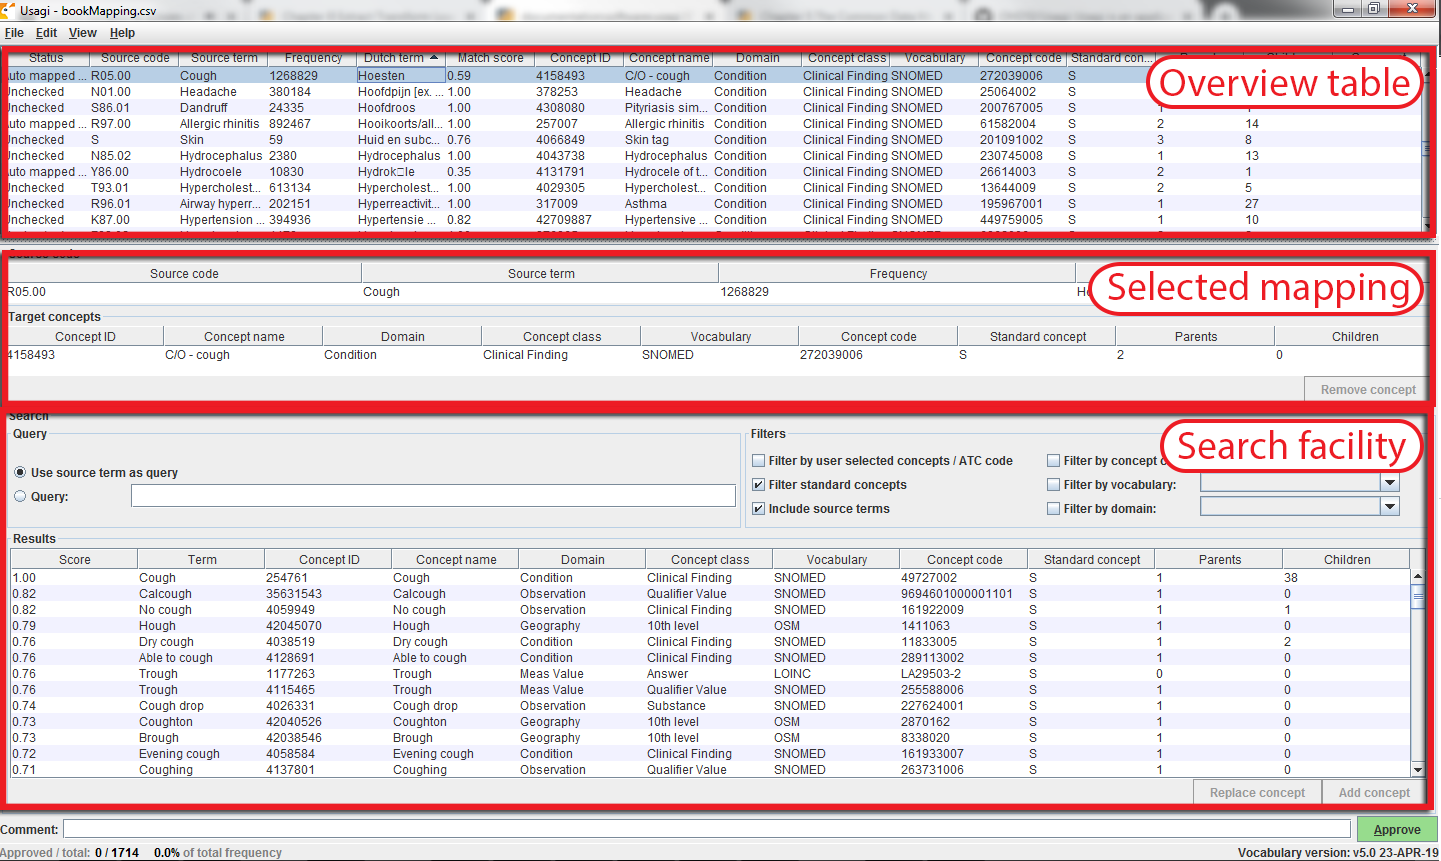
\includegraphics[width=1\linewidth]{images/ExtractTransformLoad/usagiOverview} 

}

\caption{Usagi source code input screen.}\label{fig:usagiOverview}
\end{figure}

\subsubsection*{Approuver un Mapping Suggéré}\label{approuver-un-mapping-sugguxe9ruxe9}
\addcontentsline{toc}{subsubsection}{Approuver un Mapping Suggéré}

Le ``Tableau d'aperçu'' montre le mapping actuel des codes source aux concepts. Juste après avoir importé les codes source, ce mapping contient les mappings suggérés automatiquement basés sur la similarité de termes et toute option de recherche. Dans l'exemple de la figure \ref{fig:usagiOverview}, les noms anglais des codes de condition néerlandais ont été mappés à des concepts standards dans le domaine Condition, car l'utilisateur a restreint la recherche à ce domaine. Usagi a comparé les descriptions des codes source aux noms et synonymes des concepts pour trouver la meilleure correspondance. Parce que l'utilisateur avait sélectionné ``Include source terms'', Usagi a également pris en compte les noms et synonymes de tous les concepts source dans le vocabulaire qui mappent à un concept particulier. Si Usagi est incapable de faire un mapping, il le mappera au CONCEPT\_ID = 0.

Il est suggéré qu'une personne ayant de l'expérience avec les systèmes de codage aide à mapper les codes source à leur vocabulaire standard associé. Cette personne travaillera code par code dans le ``Tableau d'aperçu'' pour soit accepter le mapping suggéré par Usagi, soit choisir un nouveau mapping. Par exemple, dans la figure \ref{fig:usagiOverview}, nous voyons que le terme néerlandais ``Hoesten'' qui a été traduit par ``Cough''. Usagi a utilisé ``Cough'' et l'a mappé au concept du Vocabulaire ``4158493-C/O - cough''. Il y avait un score de correspondance de 0.58 associé à cette paire de correspondance (les scores de correspondance sont généralement de 0 à 1, 1 étant une correspondance confiante), un score de 0.58 signifie qu'Usagi n'est pas très certain de la qualité du mapping de ce code néerlandais à SNOMED. Supposons que dans ce cas, nous soyons d'accord avec ce mapping, nous pouvons l'approuver en cliquant sur le bouton vert ``Approve'' en bas à droite de l'écran.

\subsubsection*{Rechercher un Nouveau Mapping}\label{rechercher-un-nouveau-mapping}
\addcontentsline{toc}{subsubsection}{Rechercher un Nouveau Mapping}

Il y aura des cas où Usagi suggère un mapping et l'utilisateur devra soit essayer de trouver un meilleur mapping soit définir le mapping à aucun concept (CONCEPT\_ID = 0). Dans l'exemple donné dans la figure \ref{fig:usagiOverview}, nous voyons pour le terme néerlandais ``Hoesten'', qui a été traduit par ``Cough''. La suggestion d'Usagi était restreinte par le concept identifié dans notre mapping dérivé automatiquement d'UMLS, et le résultat peut ne pas être optimal. Dans l'outil de recherche, nous pourrions rechercher d'autres concepts en utilisant soit le terme lui-même, soit une requête de boîte de recherche.

Lors de l'utilisation de la boîte de recherche manuelle, il faut garder à l'esprit qu'Usagi utilise une recherche floue, et ne prend pas en charge les requêtes de recherche structurée, par exemple ne supportant pas les opérateurs booléens comme AND et OR.

Pour continuer notre exemple, supposons que nous avons utilisé le terme de recherche ``Cough'' pour voir si nous pouvions trouver un meilleur mapping. À droite de la section Query de l'outil de recherche, il y a une section Filters, cela fournit des options pour réduire les résultats du Vocabulaire lors de la recherche du terme recherché. Dans ce cas, nous savons que nous voulons seulement trouver des concepts standards, et nous permettons que des concepts soient trouvés en fonction des noms et synonymes des concepts source dans le vocabulaire qui mappent à ces concepts standards.

Lorsque nous appliquons ces critères de recherche, nous trouvons ``254761-Cough'' et estimons que cela peut être un concept de Vocabulaire approprié à mapper à notre code néerlandais. Pour ce faire, nous pouvons cliquer sur le bouton ``Replace concept'', qui se mettra à jour dans la section ``Selected Source Code'', suivi du bouton ``Approve''. Il y a aussi un bouton ``Add concept'', qui permet de mapper plusieurs concepts de Vocabulaire standard à un seul code source (par exemple, certains codes source peuvent regrouper plusieurs maladies tandis que le vocabulaire standard peut ne pas le faire).

\subsubsection*{Informations sur le Concept}\label{informations-sur-le-concept}
\addcontentsline{toc}{subsubsection}{Informations sur le Concept}

Lors de la recherche de concepts appropriés à mapper, il est important de considérer la ``vie sociale'' d'un concept. La signification d'un concept pourrait dépendre en partie de sa place dans la hiérarchie, et parfois il y a des ``concepts orphelins'' dans le vocabulaire avec peu ou pas de relations hiérarchiques, qui seraient mal adaptés comme concepts cibles. Usagi rapportera souvent le nombre de parents et d'enfants qu'un concept a, et il est également possible de montrer plus d'informations en appuyant sur ALT + C ou en sélectionnant view --\textgreater{} Concept information dans la barre de menu supérieure.

\begin{figure}

{\centering 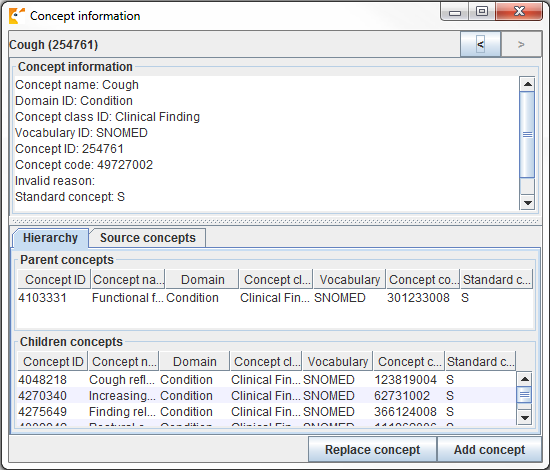
\includegraphics[width=1\linewidth]{images/ExtractTransformLoad/usagiConceptInfo} 

}

\caption{Usagi concept information panel.}\label{fig:usagiConceptInfo}
\end{figure}

La figure \ref{fig:usagiConceptInfo} montre le panneau d'informations sur le concept. Il montre des informations générales sur un concept, ainsi que ses parents, enfants et autres codes source qui mappent à ce concept. Les utilisateurs peuvent utiliser ce panneau pour naviguer dans la hiérarchie et potentiellement choisir un autre concept cible.

Continuez à suivre ce processus, code par code, jusqu'à ce que tous les codes aient été vérifiés. Dans la liste des codes source en haut de l'écran, en sélectionnant l'en-tête de colonne, vous pouvez trier les codes. Souvent, nous suggérons de passer des codes les plus fréquents aux moins fréquents. En bas à gauche de l'écran, vous pouvez voir le nombre de codes avec des mappings approuvés, et combien d'occurrences de code cela représente.

Il est possible d'ajouter des commentaires aux mappings, ce qui pourrait être utilisé pour documenter pourquoi une décision de mapping a été prise.

\subsubsection*{Meilleures Pratiques}\label{meilleures-pratiques}
\addcontentsline{toc}{subsubsection}{Meilleures Pratiques}

\begin{itemize}
\tightlist
\item
  Utilisez quelqu'un qui a de l'expérience avec les schémas de codage.
\item
  En cliquant sur un nom de colonne, vous pouvez trier les colonnes dans le ``Tableau d'aperçu''. Il peut être utile de trier sur ``Match Score''; examiner les codes qu'Usagi est le plus confiant peut rapidement éliminer une partie importante des codes. Le tri sur ``Frequency'' est également précieux, consacrer plus d'efforts aux codes fréquents par rapport aux codes non fréquents est important.
\item
  Il est acceptable de mapper certains codes à CONCEPT\_ID = 0, certains codes peuvent ne pas valoir la peine de trouver un bon mapping et d'autres peuvent simplement manquer d'un mapping approprié.
\item
  Il est important de considérer le contexte d'un concept, notamment ses parents et enfants.
\end{itemize}

\subsubsection*{Exporter le Mapping Créé par Usagi}\label{exporter-le-mapping-cruxe9uxe9-par-usagi}
\addcontentsline{toc}{subsubsection}{Exporter le Mapping Créé par Usagi}

Une fois que vous avez créé votre mapping dans USAGI, la meilleure façon de l'utiliser à l'avenir est de l'exporter et de l'ajouter à la table SOURCE\_TO\_CONCEPT\_MAP du Vocabulaire.

Pour exporter vos mappings, allez à File --\textgreater{} Export source\_to\_concept\_map. Une fenêtre contextuelle apparaîtra vous demandant quel SOURCE\_VOCABULARY\_ID vous souhaitez utiliser, tapez un identifiant court. Usagi utilisera cet identifiant comme SOURCE\_VOCABULARY\_ID qui vous permettra d'identifier votre mapping spécifique dans la table SOURCE\_TO\_CONCEPT\_MAP.

Après avoir sélectionné le SOURCE\_VOCABULARY\_ID, donnez un nom à votre CSV exporté et enregistrez-le à l'emplacement souhaité. La structure du CSV exporté est celle de la table SOURCE\_TO\_CONCEPT\_MAP. Ce mapping pourrait être ajouté à la table SOURCE\_TO\_CONCEPT\_MAP du Vocabulaire. Il serait également logique d'ajouter une seule ligne à la table VOCABULARY définissant le SOURCE\_VOCABULARY\_ID que vous avez défini ci-dessus. Enfin, il est important de noter que seuls les mappings avec le statut ``Approved'' seront exportés dans le fichier CSV ; le mapping doit être terminé dans USAGI pour être exporté.

\subsubsection*{Mettre à Jour un Mapping Usagi}\label{mettre-uxe0-jour-un-mapping-usagi}
\addcontentsline{toc}{subsubsection}{Mettre à Jour un Mapping Usagi}

Souvent, un mapping n'est pas un effort unique. Les données étant mises à jour, de nouveaux codes source sont peut-être ajoutés, et le vocabulaire est mis à jour régulièrement, nécessitant peut-être une mise à jour du mapping.

Lorsque l'ensemble des codes source est mis à jour, les étapes suivantes peuvent supporter la mise à jour :

\begin{enumerate}
\def\labelenumi{\arabic{enumi}.}
\tightlist
\item
  Importez le nouveau fichier de codes source.
\item
  Sélectionnez File --\textgreater{} Apply previous mapping, et sélectionnez l'ancien fichier de mapping Usagi.
\item
  Identifiez les codes qui n'ont pas hérité des mappings approuvés de l'ancien mapping, et mappez-les comme d'habitude.
\end{enumerate}

Lorsque le vocabulaire est mis à jour, suivez ces étapes :

\begin{enumerate}
\def\labelenumi{\arabic{enumi}.}
\tightlist
\item
  Téléchargez les nouveaux fichiers de vocabulaire depuis Athena.
\item
  Reconstruisez l'index Usagi (Help --\textgreater{} Rebuild index).
\item
  Ouvrez le fichier de mapping.
\item
  Identifiez les codes qui se mappent à des concepts qui, dans la nouvelle version du vocabulaire, ne sont plus des Concepts Standards, et trouvez des cibles de concepts plus appropriées.
  \#\# Étape 3 : Mettre en œuvre l'ETL
\end{enumerate}

Une fois que les mappings de conception et de code sont complétés, le processus ETL peut être mis en œuvre dans un logiciel. Lors de la conception de l'ETL, nous avons recommandé que des personnes connaissant bien la source et le CDM travaillent ensemble sur la tâche. De même, lors de la mise en œuvre de l'ETL, il est préférable d'utiliser des personnes ayant de l'expérience avec le travail sur des données (en particulier de grandes données) et avec la mise en œuvre d'ETL. Cela peut signifier travailler avec des personnes en dehors de votre groupe immédiat ou embaucher des consultants techniques pour exécuter la mise en œuvre. Il est également important de noter que ce n'est pas une dépense ponctuelle. À l'avenir, il serait bon d'avoir une personne ou une équipe qui consacre au moins une partie de son temps à la maintenance et à l'exécution de l'ETL (cela deviendra plus clair dans la section \ref{CDMandETLMaintenance}).

La mise en œuvre varie généralement d'un site à l'autre et dépend largement de nombreux facteurs, notamment l'infrastructure, la taille de la base de données, la complexité de l'ETL, et l'expertise technique disponible. Parce que cela dépend de nombreux facteurs, la communauté OHDSI ne fait pas de recommandation formelle sur la meilleure manière de mettre en œuvre un ETL. Certains groupes utilisent des constructeurs SQL simples, SAS, C\#, Java et Kettle. Tous ont leurs avantages et inconvénients, et aucun n'est utilisable s'il n'y a personne sur le site qui connaît la technologie.

Quelques exemples de différents ETL (classés par ordre de complexité) :\index{ETL!implémentations}

\begin{itemize}
\tightlist
\item
  ETL-Synthea - Un constructeur SQL écrit pour convertir la base de données Synthea

  \begin{itemize}
  \tightlist
  \item
    \url{https://github.com/OHDSI/etl-synthea}
  \end{itemize}
\item
  ETL-CDMBuilder - Une application .NET conçue pour transformer plusieurs bases de données

  \begin{itemize}
  \tightlist
  \item
    \url{https://github.com/OHDSI/etl-cdmbuilder}
  \end{itemize}
\item
  ETL-LambdaBuilder - Un constructeur utilisant la fonctionnalité AWS lambda

  \begin{itemize}
  \tightlist
  \item
    \url{https://github.com/OHDSI/etl-lambdabuilder}
  \end{itemize}
\end{itemize}

Il convient de noter qu'après plusieurs tentatives indépendantes, nous avons abandonné le développement de l'outil ETL `ultime' convivial. Il est toujours vrai que des outils comme celui-ci fonctionnent bien pour 80\% de l'ETL, mais pour les 20\% restants de l'ETL, un code de bas niveau doit être écrit spécifiquement pour une base de données source.

Une fois que les personnes techniques sont prêtes à commencer la mise en œuvre, le document de conception ETL doit leur être partagé. Il devrait y avoir suffisamment d'informations dans la documentation pour qu'ils puissent commencer, mais il est à prévoir que les développeurs aient accès aux concepteurs ETL pour poser des questions pendant leur processus de développement. La logique qui peut être claire pour les concepteurs peut être moins claire pour un implémenteur qui pourrait ne pas être familier avec les données et le CDM. La phase de mise en œuvre doit rester un effort d'équipe. Il est considéré comme une pratique acceptable de passer par le processus de création et de test du CDM entre les implémenteurs et les concepteurs, respectivement, jusqu'à ce que les deux groupes soient d'accord pour dire que toute la logique a été exécutée correctement.

\section{Étape 4 : Contrôle de Qualité}\label{uxe9tape-4-contruxf4le-de-qualituxe9}

Pour le processus extract, transform, load, le contrôle de qualité est itératif. Le schéma typique est de rédiger la logique -\textgreater{} implémenter la logique -\textgreater{} tester la logique -\textgreater{} corriger/rédiger la logique. Il existe de nombreuses façons de tester un CDM, mais ci-dessous se trouvent des étapes recommandées qui ont été développées à travers la communauté au fil des années de mise en œuvre d'ETL. \index{ETL!contrôle de qualité}

\begin{itemize}
\tightlist
\item
  Examiner le document de conception ETL, le code informatique et les mappings de code. Toute personne peut faire des erreurs, donc au moins une autre personne doit toujours examiner ce qui a été fait.

  \begin{itemize}
  \tightlist
  \item
    Les plus gros problèmes dans le code informatique proviennent généralement de la manière dont les codes source dans les données natives sont mappés aux Concepts Standard. Le mapping peut devenir délicat, notamment lorsqu'il s'agit de codes spécifiques à une date comme les NDC. Assurez-vous de vérifier deux fois toute zone où des mappings sont effectués pour garantir que les vocabulaires sources corrects sont traduits en concept\_id approprié.
  \end{itemize}
\item
  Comparer manuellement toutes les informations sur un échantillon de personnes dans les données sources et cibles.

  \begin{itemize}
  \tightlist
  \item
    Il peut être utile de passer en revue les données d'une personne, idéalement une personne avec un grand nombre d'enregistrements uniques. Suivre les données d'une seule personne peut mettre en lumière des problèmes si les données dans le CDM ne sont pas telles que vous vous attendiez à les voir en fonction de la logique convenue.
  \end{itemize}
\item
  Comparer les décomptes globaux dans les données sources et cibles.

  \begin{itemize}
  \tightlist
  \item
    Il peut y avoir certaines différences attendues dans les décomptes selon la manière dont vous avez choisi de traiter certains problèmes. Par exemple, certains collaborateurs choisissent de supprimer toute personne ayant un sexe NULL, car ces personnes ne seront de toute façon pas incluses dans les analyses. Il peut également être le cas que les visites dans le CDM soient construites différemment des visites ou rencontres dans les données natives. Par conséquent, lors de la comparaison des décomptes globaux entre les données sources et le CDM, assurez-vous de tenir compte de ces différences et de les attendre.
  \end{itemize}
\item
  Reproduire une étude qui a déjà été réalisée sur les données sources dans la version CDM.

  \begin{itemize}
  \tightlist
  \item
    C'est un bon moyen de comprendre toute différence majeure entre les données sources et la version CDM, bien que cela soit un peu plus chronophage.
  \end{itemize}
\item
  Créer des tests unitaires destinés à reproduire un schéma dans les données sources qui doit être pris en compte dans l'ETL. Par exemple, si votre ETL spécifie que les patients sans information sur le sexe doivent être supprimés, créez un test unitaire d'une personne sans sexe et évaluez la manière dont le constructeur le gère.

  \begin{itemize}
  \tightlist
  \item
    Les tests unitaires sont très pratiques pour évaluer la qualité et l'exactitude d'une conversion ETL. Ils impliquent généralement de créer un ensemble de données beaucoup plus petit qui imite la structure des données sources que vous êtes en train de convertir. Chaque personne ou enregistrement de l'ensemble de données doit tester un élément spécifique de la logique tel qu'écrit dans le document ETL. En utilisant cette méthode, il est facile de retracer les problèmes et d'identifier la logique défaillante. La petite taille permet également au code informatique de s'exécuter très rapidement, ce qui permet des itérations et une identification des erreurs plus rapides.
  \end{itemize}
\end{itemize}

Ce sont des moyens de haut niveau pour aborder le contrôle de la qualité du point de vue d'un ETL. Pour plus de détails sur les efforts de qualité des données en cours au sein de l'OHDSI, veuillez consulter le chapitre \ref{DataQuality}.

\section{Conventions ETL et THEMIS}\label{conventions-etl-et-themis}

Au fur et à mesure que de nombreux groupes convertissaient des données au CDM, il est apparu clairement que des conventions devaient être spécifiées. Par exemple, que doit faire l'ETL dans une situation où un enregistrement de personne manque d'année de naissance ? L'objectif du CDM est de standardiser les données de santé ; cependant, si chaque groupe traite les scénarios de données spécifiques différemment, il devient plus difficile d'utiliser systématiquement les données à travers le réseau.

La communauté OHDSI a commencé à documenter des conventions pour améliorer la cohérence entre les CDM. Ces conventions définies, sur lesquelles la communauté OHDSI s'est mise d'accord, peuvent être trouvées sur le Wiki CDM.\footnote{\url{https://github.com/OHDSI/CommonDataModel/wiki}{]}.} Chaque table du CDM a son propre ensemble de conventions auxquelles se référer lors de la conception d'un ETL. Par exemple, les personnes peuvent manquer de mois ou de jour de naissance, mais si elles manquent d'année de naissance, la personne doit être supprimée. En concevant un ETL, référez-vous aux conventions pour vous aider à prendre certaines décisions de conception qui seront compatibles avec la communauté.

Bien qu'il ne soit jamais possible de documenter tous les scénarios de données possibles qui existent et quoi faire lorsqu'ils se produisent, il existe un groupe de travail OHDSI qui essaie de documenter les scénarios communs. THEMIS\footnote{\url{https://github.com/OHDSI/Themis}} est composé de personnes de la communauté qui rassemblent des conventions, les clarifient, les partagent avec la communauté pour commentaires, puis documentent les conventions finalisées dans le Wiki CDM. THEMIS est une ancienne Titanide grecque de l'ordre divin, de l'équité, de la loi, de la loi naturelle et de la coutume, ce qui semblait bien correspondre à la mission de ce groupe. Lors de la réalisation d'un ETL, si un scénario vous met dans l'incertitude de la manière de le gérer, THEMIS recommande de poser une question à ce sujet sur les forums OHDSI.\footnote{\url{http://forums.ohdsi.org/}} Il est très probable que si vous avez une question, d'autres membres de la communauté l'ont probablement aussi. THEMIS utilise ces discussions, ainsi que les réunions de groupe de travail et les discussions en face à face, pour aider à informer des autres conventions qui doivent être documentées.

\section{Maintenance du CDM et de l'ETL}\label{CDMandETLMaintenance}

Concevoir l'ETL, créer les mappings, implémenter l'ETL et mettre en place des mesures de contrôle de qualité demande un effort considérable. Malheureusement, l'effort ne s'arrête pas là. Il existe un cycle de maintenance de l'ETL qui est un processus continu après la construction du premier CDM. Certains déclencheurs courants nécessitant une maintenance sont : des changements dans les données sources, un bogue dans l'ETL, une nouvelle version des vocabulaires OMOP, ou des modifications ou mises à jour du CDM lui-même. Si l'un de ces déclencheurs se produit, les éléments suivants pourraient nécessiter une mise à jour : la documentation de l'ETL, le logiciel exécutant l'ETL, les cas de test et les contrôles de qualité.

Souvent, une source de données de santé change constamment. De nouvelles données peuvent être disponibles (par exemple, une nouvelle colonne dans les données peut exister). Des scénarios de patients qui n'existaient pas auparavant peuvent soudainement apparaître (par exemple, un nouveau patient qui a un acte de décès avant sa naissance). Votre compréhension des données peut s'améliorer (par exemple, certains dossiers d'accouchement hospitalier peuvent être classés en tant qu'ambulatoires en raison de la manière dont les réclamations sont traitées). Toutes les modifications des données sources ne déclenchent pas nécessairement un changement dans le traitement ETL, cependant au minimum, les modifications qui cassent le traitement ETL devront être abordées.

Si des bogues sont découverts, ils doivent être corrigés. Cependant, il est important de garder à l'esprit que tous les bogues ne sont pas créés égaux. Par exemple, disons que dans la table COST, la colonne coût était arrondie à un chiffre entier (par exemple, les données sources avaient 3,82 \$ et cela devenait 4,00 \$ dans le CDM). Si les principaux chercheurs utilisant les données faisaient principalement des caractérisations des expositions médicamenteuses et des conditions des patients, un bogue tel que celui-ci a peu d'importance et peut être corrigé à l'avenir. Si les principaux chercheurs utilisant les données incluaient également des économistes de la santé, cela serait un bogue critique qui devrait être corrigé immédiatement.

Le Vocabulaire OMOP change également en permanence tout comme nos données sources peuvent le faire. En fait, le vocabulaire peut avoir plusieurs versions dans un même mois à mesure que les vocabulaires sont mis à jour. Chaque CDM est exécuté sur une version spécifique d'un vocabulaire et l'exécution sur un vocabulaire plus récent et amélioré pourrait entraîner des changements dans la façon dont les codes sources sont mappés aux vocabulaires standardisés. Souvent, les différences entre les vocabulaires sont mineures, donc construire un nouveau CDM chaque fois qu'une nouvelle version du vocabulaire est publiée n'est pas nécessaire. Cependant, il est bon de pratiquer l'adoption d'un nouveau vocabulaire une ou deux fois par an, ce qui nécessiterait de traiter à nouveau le CDM. Il est rare que des changements dans une nouvelle version d'un vocabulaire nécessitent que le code ETL soit lui-même mis à jour.

Le dernier déclencheur pouvant nécessiter une maintenance du CDM ou de l'ETL est lorsque le modèle de données commun lui-même est mis à jour. À mesure que la communauté grandit et que de nouveaux besoins en données sont trouvés, cela peut conduire à l'ajout de nouvelles données dans le CDM. Cela peut signifier que des données que vous ne stockiez pas auparavant dans le CDM pourraient trouver un emplacement dans une nouvelle version du CDM. Les changements de structure existante du CDM sont moins fréquents, mais c'est une possibilité. Par exemple, le CDM a adopté des champs DATETIME au lieu des champs DATE originaux, ce qui pourrait causer une erreur dans le traitement ETL. Les versions du CDM ne sont pas publiées fréquemment et les sites peuvent choisir quand migrer.

\section{Réflexions finales sur l'ETL}\label{ruxe9flexions-finales-sur-letl}

Le processus ETL est difficile pour de nombreuses raisons, dont la moindre n'est pas le fait que nous traitons tous des données sources uniques, rendant difficile la création d'une solution ``taille unique''. Cependant, au fil des années, nous avons appris les leçons suivantes durement acquises.

\begin{itemize}
\tightlist
\item
  La règle des 80/20. Si vous pouvez l'éviter, ne passez pas trop de temps à mapper manuellement les codes sources aux ensembles de concepts. Idéalement, mappez les codes sources qui couvrent la majorité de vos données. Cela devrait suffire pour vous lancer et vous pourrez traiter les codes restants à l'avenir en fonction des cas d'utilisation.
\item
  Il est acceptable de perdre des données qui ne sont pas de qualité pour la recherche. Souvent, ce sont les dossiers qui seraient écartés avant de commencer une analyse de toute façon, nous les supprimons simplement pendant le processus ETL à la place.
\item
  Un CDM nécessite une maintenance. Ce n'est pas parce que vous terminez une ETL que vous n'avez plus jamais besoin d'y toucher. Vos données brutes peuvent changer, il peut y avoir un bogue dans le code, il peut y avoir un nouveau vocabulaire ou une mise à jour du CDM. Prévoyez d'allouer des ressources pour ces changements afin que votre ETL soit toujours à jour.
\item
  Pour obtenir de l'aide pour démarrer le CDM OHDSI, effectuer votre conversion de base de données ou exécuter les outils d'analyses, veuillez visiter notre Forum des Implémenteurs.\footnote{\url{https://forums.ohdsi.org/c/implementers}}
\end{itemize}

\section{Résumé}\label{ruxe9sumuxe9-4}

\begin{rmdsummary}
\begin{itemize}
\item
  Il existe un processus généralement accepté pour aborder un ETL, incluant

  \begin{itemize}
  \tightlist
  \item
    Les experts en données et les experts en CDM conçoivent ensemble l'ETL
  \item
    Les personnes ayant des connaissances médicales créent les mappings de codes
  \item
    Une personne technique met en œuvre l'ETL
  \item
    Tous sont impliqués dans le contrôle de qualité
  \end{itemize}
\item
  Des outils ont été développés par la communauté OHDSI pour faciliter ces étapes et sont disponibles gratuitement
\item
  Il existe de nombreux exemples d'ETL et des conventions acceptées que vous pouvez utiliser comme guide
\end{itemize}
\end{rmdsummary}

\section{Exercices}\label{exercices-2}

\begin{exercise}
\protect\hypertarget{exr:exerciseEtl1}{}\label{exr:exerciseEtl1}

Mettez les étapes du processus ETL dans le bon ordre :

\begin{enumerate}
\def\labelenumi{\Alph{enumi})}
\tightlist
\item
  Les experts en données et les experts en CDM conçoivent ensemble l'ETL
\item
  Une personne technique met en œuvre l'ETL
\item
  Les personnes ayant des connaissances médicales créent les mappings de codes
\item
  Tous sont impliqués dans le contrôle de qualité
\end{enumerate}

\end{exercise}

\begin{exercise}
\protect\hypertarget{exr:exerciseEtl2}{}\label{exr:exerciseEtl2}

En utilisant les ressources OHDSI de votre choix, repérez quatre problèmes avec l'enregistrement PERSON montré dans le tableau \ref{tab:exercisePersonTable} (tableau abrégé pour l'espace) :

\begin{longtable}[]{@{}ll@{}}
\caption{\label{tab:exercisePersonTable} Une table PERSON.}\tabularnewline
\toprule\noalign{}
Colonne & Valeur \\
\midrule\noalign{}
\endfirsthead
\toprule\noalign{}
Colonne & Valeur \\
\midrule\noalign{}
\endhead
\bottomrule\noalign{}
\endlastfoot
PERSON\_ID & A123B456 \\
GENDER\_CONCEPT\_ID & 8532 \\
YEAR\_OF\_BIRTH & NULL \\
MONTH\_OF\_BIRTH & NULL \\
DAY\_OF\_BIRTH & NULL \\
RACE\_CONCEPT\_ID & 0 \\
ETHNICITY\_CONCEPT\_ID & 8527 \\
PERSON\_SOURCE\_VALUE & A123B456 \\
GENDER\_SOURCE\_VALUE & F \\
RACE\_SOURCE\_VALUE & WHITE \\
ETHNICITY\_SOURCE\_VALUE & NONE PROVIDED \\
\end{longtable}

\end{exercise}

\begin{exercise}
\protect\hypertarget{exr:exerciseEtl3}{}\label{exr:exerciseEtl3}Essayons de générer des enregistrements VISIT\_OCCURRENCE. Voici une logique d'exemple écrite pour Synthea :
Triez les données par ordre croissant par PATIENT, START, END. Puis par PERSON\_ID, fusionnez les lignes de réclamation tant que le délai entre la FIN d'une ligne et le DÉBUT de la suivante est \textless=1 jour. Chaque réclamation hospitalière consolidée est alors considérée comme une seule visite hospitalière, définissez :

\begin{itemize}
\tightlist
\item
  MIN(START) comme VISIT\_START\_DATE
\item
  MAX(END) comme VISIT\_END\_DATE
\item
  ``IP'' comme PLACE\_OF\_SERVICE\_SOURCE\_VALUE
\end{itemize}

Si vous voyez un ensemble de visites comme montré dans la Figure \ref{fig:exerciseSourceData} dans vos données sources, comment vous attendez-vous à ce que l'enregistrement VISIT\_OCCURRENCE résultant se présente dans le CDM ?
\end{exercise}

\begin{figure}

{\centering 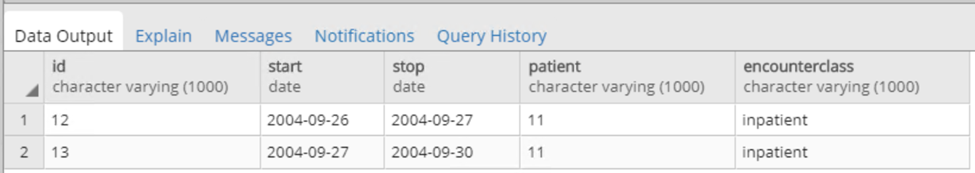
\includegraphics[width=1\linewidth]{images/ExtractTransformLoad/exerciseSourceData} 

}

\caption{Example source data.}\label{fig:exerciseSourceData}
\end{figure}

Les réponses suggérées se trouvent dans l'Appendice \ref{Etlanswers}.

\part{Analyse des Données}\label{part-analyse-des-donnuxe9es}

\chapter{Cas d'utilisation de l'analyse des données}\label{DataAnalyticsUseCases}

\emph{Responsable du chapitre : David Madigan}

La collaboration OHDSI se concentre sur la génération de preuves fiables à partir des données réelles de soins de santé, généralement sous forme de bases de données de réclamations ou de dossiers de santé électroniques. Les cas d'utilisation sur lesquels OHDSI se concentre se répartissent en trois grandes catégories :

\begin{itemize}
\tightlist
\item
  Caractérisation
\item
  Estimation au niveau de la population
\item
  Prédiction au niveau du patient
\end{itemize}

Nous décrivons ces éléments en détail ci-dessous. Notez que pour tous les cas d'utilisation, les preuves que nous générons héritent des limitations des données ; nous discutons de ces limitations en détail dans la section du livre sur la qualité des preuves (Chapitres \ref{EvidenceQuality} - \ref{MethodValidity}).

\section{Caractérisation}\label{caractuxe9risation}

\index{caractérisation}

La caractérisation tente de répondre à la question :

\begin{quote}
Qu'est-ce qui leur est arrivé ?
\end{quote}

Nous pouvons utiliser les données pour répondre à des questions sur les caractéristiques des personnes dans une cohorte ou l'ensemble de la base de données, la pratique des soins de santé, et étudier comment ces choses changent au fil du temps.

Les données peuvent fournir des réponses à des questions telles que :

\begin{itemize}
\tightlist
\item
  Pour les patients nouvellement diagnostiqués avec fibrillation auriculaire, combien reçoivent une prescription de warfarine ?
\item
  Quel est l'âge moyen des patients qui subissent une arthroplastie de la hanche ?
\item
  Quel est le taux d'incidence de la pneumonie chez les patients de plus de 65 ans ?
\end{itemize}

Les questions typiques de caractérisation sont formulées comme suit :

\begin{itemize}
\tightlist
\item
  Combien de patients\ldots{} ?
\item
  À quelle fréquence\ldots{} ?
\item
  Quelle proportion de patients\ldots{} ?
\item
  Quelle est la distribution des valeurs pour le laboratoire\ldots{} ?
\item
  Quels sont les niveaux d'HbA1c pour les patients avec\ldots{} ?
\item
  Quelles sont les valeurs de laboratoire pour les patients\ldots{} ?
\item
  Quelle est la durée médiane d'exposition pour les patients sous\ldots{} ?
\item
  Quelles sont les tendances au fil du temps dans\ldots{} ?
\item
  Quels sont les autres médicaments que ces patients utilisent ?
\item
  Quelles sont les thérapies concomitantes ?
\item
  Avons-nous suffisamment de cas de\ldots{} ?
\item
  Serait-il faisable d'étudier X\ldots{} ?
\item
  Quelles sont les caractéristiques démographiques de\ldots{} ?
\item
  Quels sont les facteurs de risque de\ldots{} ? (si identifiant un facteur de risque spécifique, peut-être estimation, pas prédiction)
\item
  Quels sont les prédicteurs de\ldots{} ?
\end{itemize}

Et la sortie désirée est :

\begin{itemize}
\tightlist
\item
  Nombre ou pourcentage
\item
  Moyennes
\item
  Statistiques descriptives
\item
  Taux d'incidence
\item
  Prévalence
\item
  Cohorte
\item
  Phénotype basé sur des règles
\item
  Utilisation des médicaments
\item
  Histoire naturelle de la maladie
\item
  Adhérence
\item
  Profil de comorbidités
\item
  Voies de traitement
\item
  Ligne de thérapie
\end{itemize}

\section{Estimation Au Niveau De La Population}\label{estimation-au-niveau-de-la-population}

\index{estimation au niveau de la population}

Dans une certaine mesure, les données peuvent soutenir des inférences causales sur les effets des interventions de santé, en répondant à la question

\begin{quote}
Quels sont les effets causaux ?
\end{quote}

Nous aimerions comprendre les effets causaux pour comprendre les conséquences des actions. Par exemple, si nous décidons de prendre un traitement, comment cela change-t-il ce qui nous arrive à l'avenir ?

Les données peuvent fournir des réponses à des questions telles que :

\begin{itemize}
\tightlist
\item
  Pour les patients nouvellement diagnostiqués avec fibrillation auriculaire, dans la première année après le début de la thérapie, la warfarine provoque-t-elle plus d'hémorragies majeures que le dabigatran ?
\item
  L'effet causal de la metformine sur la diarrhée varie-t-il en fonction de l'âge ?
\end{itemize}

Les questions typiques de l'estimation des effets au niveau de la population sont formulées comme suit :

\begin{itemize}
\tightlist
\item
  Quel est l'effet de\ldots{} ?
\item
  Que se passe-t-il si je fais l'intervention\ldots{} ?
\item
  Quel traitement fonctionne mieux ?
\item
  Quel est le risque de X sur Y ?
\item
  Quel est le délai avant l'événement de\ldots{} ?
\end{itemize}

Et la sortie désirée est :

\begin{itemize}
\tightlist
\item
  Risque relatif
\item
  Ratio de hasards
\item
  Ratio de cotes
\item
  Effet moyen du traitement
\item
  Effet causal
\item
  Association
\item
  Corrélation
\item
  Surveillance de la sécurité
\item
  Efficacité comparative
\end{itemize}

\section{Prédiction Au Niveau Du Patient}\label{pruxe9diction-au-niveau-du-patient}

\index{prédiction au niveau du patient}

Basé sur les antécédents de santé du patient collectés dans la base de données, nous pouvons faire des prédictions au niveau du patient sur de futurs événements de santé, répondant à la question

\begin{quote}
Que va-t-il m'arriver ?
\end{quote}

Les données peuvent fournir des réponses à des questions telles que :

\begin{itemize}
\tightlist
\item
  Pour un patient spécifique nouvellement diagnostiqué avec un trouble dépressif majeur, quelle est la probabilité que le patient tente de se suicider dans la première année suivant le diagnostic ?
\item
  Pour un patient spécifique nouvellement diagnostiqué avec fibrillation auriculaire, dans la première année après le début de la thérapie à la warfarine, quelle est la probabilité que le patient souffre d'un accident vasculaire cérébral ischémique ?
\end{itemize}

Les questions typiques de la prédiction au niveau du patient sont formulées comme suit :

\begin{itemize}
\tightlist
\item
  Quelle est la chance que ce patient\ldots{} ?
\item
  Qui sont les candidats pour\ldots{} ?
\end{itemize}

Et la sortie désirée est :

\begin{itemize}
\tightlist
\item
  Probabilité pour un individu
\item
  Modèle de prédiction
\item
  Groupes à haut/bas risque
\item
  Phénotype probabiliste
\end{itemize}

L'estimation au niveau de la population et la prédiction au niveau du patient se chevauchent dans une certaine mesure. Par exemple, un cas d'utilisation important pour la prédiction est de prédire un résultat pour un patient spécifique si le médicament A avait été prescrit et également prédire le même résultat si le médicament B avait été prescrit. Supposons qu'en réalité, l'un de ces médicaments est prescrit (disons le médicament A) donc nous voyons si le résultat après le traitement avec A se produit effectivement. Puisque le médicament B n'a pas été prescrit, le résultat après le traitement B, bien que prévisible, est ``contrefactuel'' car il n'est jamais observé. Chacune de ces tâches de prédiction relève de la prédiction au niveau du patient. Cependant, la différence (ou le ratio) entre les deux résultats est un effet \emph{causal} au niveau de l'unité, et doit être estimé en utilisant des méthodes d'estimation des effets causaux à la place.

\begin{rmdimportant}
Les gens ont une tendance naturelle à interpréter à tort les modèles prédictifs comme s'ils étaient des modèles causaux. Mais un modèle prédictif ne peut montrer que la corrélation, jamais la causalité. Par exemple, l'utilisation de médicaments pour diabétiques pourrait être un fort prédicteur de l'infarctus du myocarde (IM) parce que le diabète est un fort facteur de risque pour l'IM. Cependant, cela ne signifie pas que l'arrêt des médicaments pour diabétiques empêchera l'IM !
\end{rmdimportant}

\section{Exemples De Cas D'utilisation Dans L'Hypertension}\label{exemples-de-cas-dutilisation-dans-lhypertension}

Vous êtes un chercheur intéressé par l'étude des effets de la monothérapie par inhibiteur de l'ECA vs.~la monothérapie par diurétique thiazidique sur les résultats de l'infarctus aigu du myocarde et de l'angioedème en tant que traitement de première ligne de l'hypertension. Vous comprenez que d'après la littérature OHDSI, vous posez une question d'estimation d'effet au niveau de la population mais d'abord, vous devez faire quelques devoirs sur la caractérisation de ce traitement particulier d'intérêt.

\subsection{Questions de Caractérisation}\label{questions-de-caractuxe9risation}

L'infarctus aigu du myocarde est une complication cardiovasculaire qui peut survenir chez les patients présentant une hypertension artérielle, de sorte qu'un traitement efficace de l'hypertension devrait réduire le risque. L'angioedème est un effet secondaire bien connu des inhibiteurs de l'ECA, qui est rare mais potentiellement grave. Vous commencez par créer des cohortes (voir Chapitre \ref{Cohorts}) pour les expositions d'intérêt (nouveaux utilisateurs d'inhibiteurs de l'ECA et nouveaux utilisateurs de diurétiques thiazidiques). Vous effectuez une analyse de caractérisation (voir Chapitre \ref{Characterization}) pour résumer les caractéristiques de base de ces populations d'exposition, y compris les conditions comorbides, et les médicaments concomitants. Vous effectuez une autre analyse de caractérisation pour estimer l'incidence de certains résultats au sein de ces populations d'exposition. Ici, vous demandez « à quelle fréquence se produisent 1) l'infarctus aigu du myocarde et 2) l'angioedème pendant la période d'exposition aux inhibiteurs de l'ECA et aux diurétiques thiazidiques ? » Ces caractérisations nous permettent d'évaluer la faisabilité de mener une étude d'estimation au niveau de la population, d'évaluer si les deux groupes de traitement sont comparables, et d'identifier les « facteurs de risque » qui pourraient prédire le choix de traitement fait par les patients.

\subsection{Question D'estimation Au Niveau De La Population}\label{question-destimation-au-niveau-de-la-population}

L'étude d'estimation des effets au niveau de la population (voir Chapitre \ref{PopulationLevelEstimation}) estime le risque relatif de l'utilisation des inhibiteurs de l'ECA vs.~des diurétiques thiazidiques pour les résultats d'IMA et d'angioedème. Ici, vous évaluez également à l'aide des diagnostics d'étude et des témoins négatifs si nous pouvons produire une estimation fiable de l'effet moyen du traitement.

\subsection{Question De Prédiction Au Niveau Du Patient}\label{question-de-pruxe9diction-au-niveau-du-patient}

Indépendamment de l'existence d'un effet causal des expositions, vous êtes également intéressé à essayer de déterminer quels patients sont les plus à risque des résultats. Il s'agit d'un problème de prédiction au niveau du patient (voir Chapitre \ref{PatientLevelPrediction}). Ici, vous développez un modèle de prédiction qui évalue : parmi les patients qui sont nouveaux utilisateurs d'inhibiteurs de l'ECA, quels patients sont les plus à risque de développer un infarctus aigu du myocarde au cours de la première année après le début du traitement. Le modèle nous permet de prédire, pour un patient qui vient de se voir prescrire un inhibiteur de l'ECA pour la première fois, en se basant sur les événements observés dans son dossier médical, quelle est la chance qu'il connaisse un IMA au cours de la prochaine année.
\#\# Limitations de la Recherche Observationnelle

\index{limitations de la recherche observationnelle}

Il y a de nombreuses questions importantes en matière de soins de santé pour lesquelles les bases de données OHDSI ne peuvent pas fournir de réponses. Celles-ci incluent :

\begin{itemize}
\tightlist
\item
  Les effets causaux des interventions comparées au placebo. Il est parfois possible de considérer l'effet causal d'un traitement par rapport à l'absence de traitement, mais pas au traitement placebo.
\item
  Tout ce qui est lié aux médicaments en vente libre.
\item
  De nombreux résultats et autres variables sont rarement enregistrés, voire pas du tout. Ceux-ci incluent la mortalité, les résultats comportementaux, le style de vie et le statut socio-économique.
\item
  Étant donné que les patients ont tendance à consulter le système de santé uniquement lorsqu'ils sont malades, il peut être difficile de mesurer les bénéfices des traitements.
\end{itemize}

\subsection{Données Erronées}\label{donnuxe9es-erronuxe9es}

Les données cliniques enregistrées dans les bases de données OHDSI peuvent dévier de la réalité clinique. Par exemple, le dossier d'un patient peut inclure un code pour infarctus du myocarde alors que le patient n'a jamais subi un infarctus du myocarde. De même, une valeur de laboratoire peut être erronée ou un code incorrect pour une procédure peut apparaître dans la base de données. Les chapitres \ref{DataQuality} et \ref{ClinicalValidity} discutent de plusieurs de ces problèmes et des bonnes pratiques visant à identifier et corriger autant que possible ces types de problèmes. Néanmoins, des données erronées persistent inévitablement dans une certaine mesure et peuvent nuire à la validité des analyses ultérieures. Une littérature extensive se concentre sur l'ajustement des inférences statistiques pour tenir compte des erreurs dans les données - voir, par exemple, \citet{fuller2009measurement}.

\subsection{Données Manquantes}\label{donnuxe9es-manquantes}

\index{données manquantes}

L'absence de données dans les bases de données OHDSI présente des défis subtils. Un événement de santé (par exemple, une ordonnance, une valeur de laboratoire, etc.) qui devrait être enregistré dans une base de données, mais ne l'est pas, est ``manquant.'' La littérature statistique distingue entre différents types de données manquantes comme ``manquantes complètement aléatoirement,'' ``manquantes aléatoirement,'' et ``manquantes non aléatoirement'' et des méthodes de complexité croissante tentent de traiter ces types. \citet{perkins2017principled} fournissent une introduction utile sur ce sujet.

\section{Résumé}\label{ruxe9sumuxe9-5}

\begin{rmdsummary}
\begin{itemize}
\item
  Dans la recherche observationnelle, nous distinguons trois grandes catégories d'études de cas.
\item
  \textbf{Caractérisation} vise à répondre à la question ``Que leur est-il arrivé ?''
\item
  \textbf{Estimation à l'échelle de la population} tente de répondre à la question ``Quels sont les effets causaux ?''
\item
  \textbf{Prédiction au niveau du patient} essaye de répondre ``Que va-t-il m'arriver ?''
\item
  Les modèles de prédiction ne sont pas des modèles causaux ; Il n'y a aucune raison de croire qu'intervenir sur un fort prédicteur impactera le résultat.
\item
  Il y a des questions qui ne peuvent pas être résolues en utilisant des données de santé observationnelles.
\end{itemize}
\end{rmdsummary}

\section{Exercices}\label{exercices-3}

\begin{exercise}
\protect\hypertarget{exr:exerciseUseCases1}{}\label{exr:exerciseUseCases1}

A quelles catégories de cas d'utilisation appartiennent ces questions ?

\begin{enumerate}
\def\labelenumi{\arabic{enumi}.}
\item
  Calculer le taux de saignement gastro-intestinal (GI) chez les patients récemment exposés aux AINS.
\item
  Calculer la probabilité qu'un patient spécifique présente un saignement GI dans l'année à venir, en fonction de ses caractéristiques initiales.
\item
  Estimer le risque accru de saignement GI dû au diclofénac comparé au célécoxib.
\end{enumerate}

\end{exercise}

\begin{exercise}
\protect\hypertarget{exr:exerciseUseCases2}{}\label{exr:exerciseUseCases2}Vous souhaitez estimer le risque accru de saignement GI dû au diclofénac comparé à l'absence d'exposition (placebo). Cela peut-il être fait en utilisant des données de santé observationnelles ?
\end{exercise}

Les réponses suggérées se trouvent dans l'Appendice \ref{UseCasesanswers}.

\chapter{Outils d'analyse d'OHDSI}\label{OhdsiAnalyticsTools}

\emph{Chefs de chapitre : Martijn Schuemie \& Frank DeFalco}

OHDSI offre une large gamme d'outils open source pour soutenir divers cas d'utilisation analytiques sur des données observationnelles au niveau des patients. Ce que ces outils ont en commun, c'est qu'ils peuvent tous interagir avec une ou plusieurs bases de données utilisant le Modèle de Données Commun (CDM). De plus, ces outils standardisent l'analyse pour divers cas d'utilisation ; plutôt que de repartir de zéro, une analyse peut être mise en œuvre en remplissant des modèles standard. Cela rend l'analyse plus facile et améliore également la reproductibilité et la transparence. Par exemple, il semble y avoir un nombre quasi infini de façons de calculer un taux d'incidence, mais ceux-ci peuvent être spécifiés dans les outils d'OHDSI avec quelques choix, et toute personne faisant ces mêmes choix calculera les taux d'incidence de la même manière.

Dans ce chapitre, nous décrivons d'abord les différentes manières dont nous pouvons choisir de mettre en œuvre une analyse, et les stratégies que l'analyse peut employer. Nous passons ensuite en revue les différents outils d'OHDSI et leur correspondance aux divers cas d'utilisation.

\section{Implémentation de l'analyse}\label{analysisImplementation}

La figure \ref{fig:implementations} montre les différentes manières dont nous pouvons choisir de mettre en œuvre une étude sur une base de données utilisant le CDM. \index{implémentation de l'analyse}

\begin{figure}

{\centering 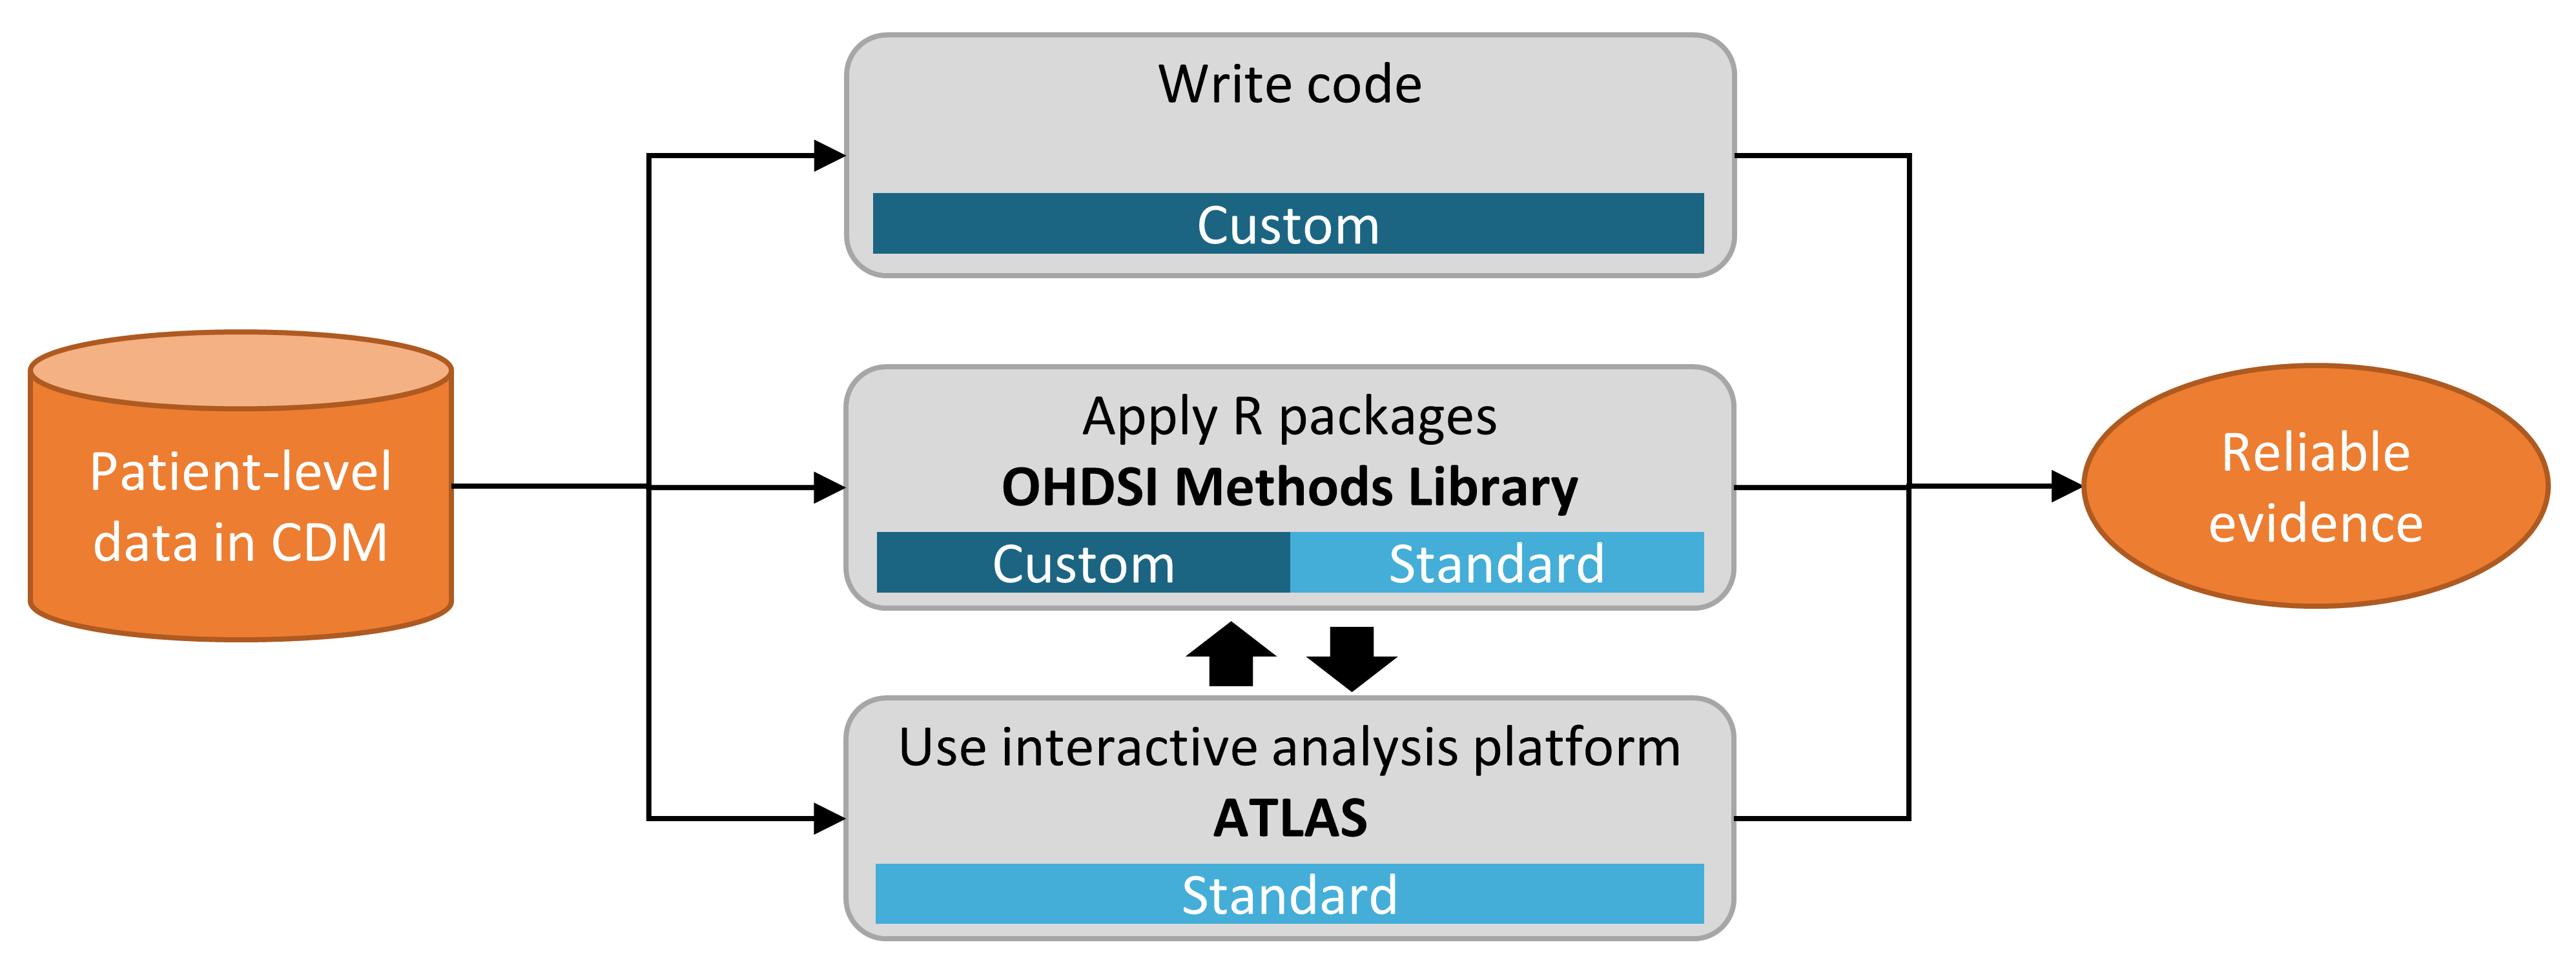
\includegraphics[width=0.9\linewidth]{images/OhdsiAnalyticsTools/implementations} 

}

\caption{Différentes manières d'implémenter une analyse sur les données du CDM.}\label{fig:implementations}
\end{figure}

Il y a principalement trois approches pour mettre en œuvre une étude. La première est d'écrire du code personnalisé qui n'utilise aucun des outils proposés par OHDSI. On pourrait écrire une analyse de novo en R, SAS, ou tout autre langage. Cela offre une flexibilité maximale et peut en fait être la seule option si l'analyse spécifique n'est prise en charge par aucun de nos outils. Cependant, cette voie nécessite beaucoup de compétences techniques, de temps et d'efforts, et à mesure que l'analyse devient plus complexe, il devient plus difficile d'éviter les erreurs dans le code.

La deuxième approche consiste à développer l'analyse en R, en utilisant les packages de la \href{https://ohdsi.github.io/MethodsLibrary/}{Bibliothèque de Méthodes d'OHDSI}. Au minimum, on pourrait utiliser les packages \href{https://ohdsi.github.io/SqlRender/}{SqlRender} et \href{https://ohdsi.github.io/DatabaseConnector/}{DatabaseConnector} décrits de manière plus détaillée dans le chapitre \ref{SqlAndR} qui permettent d'exécuter le même code sur différentes plateformes de bases de données, telles que PostgreSQL, SQL Server et Oracle. D'autres packages comme \href{https://ohdsi.github.io/CohortMethod/}{CohortMethod} et \href{https://ohdsi.github.io/PatientLevelPrediction/}{PatientLevelPrediction} offrent des fonctions R pour des analyses avancées contre le CDM qui peuvent être appelées dans son propre code. Cela nécessite toujours beaucoup d'expertise technique, mais en réutilisant les composants validés de la Bibliothèque de Méthodes, nous pouvons être plus efficaces et moins enclins à l'erreur qu'en utilisant un code totalement personnalisé.

La troisième approche repose sur notre plateforme d'analyse interactive \href{https://github.com/OHDSI/Atlas/wiki}{ATLAS}, un outil web qui permet aux non-programmeurs d'effectuer une large gamme d'analyses de manière efficace. ATLAS utilise les Bibliothèques de Méthodes mais fournit une interface graphique simple pour concevoir des analyses et, dans de nombreux cas, générer le code R nécessaire pour exécuter l'analyse. Cependant, ATLAS ne prend pas en charge toutes les options disponibles dans la Bibliothèque de Méthodes. Bien qu'il soit attendu que la majorité des études puissent être réalisées grâce à ATLAS, certaines études peuvent nécessiter la flexibilité offerte par la deuxième approche.

ATLAS et la Bibliothèque de Méthodes ne sont pas indépendants. Certaines des analyses plus complexes pouvant être invoquées dans ATLAS sont exécutées via des appels aux packages de la Bibliothèque de Méthodes. De même, les cohortes utilisées dans la Bibliothèque de Méthodes sont souvent conçues dans ATLAS.

\section{Stratégies d'analyse}\label{stratuxe9gies-danalyse}

Outre la stratégie utilisée pour mettre en œuvre notre analyse contre le CDM, par exemple via du codage personnalisé ou l'utilisation de code analytique standard dans la Bibliothèque de Méthodes, il existe également plusieurs stratégies pour utiliser ces techniques analytiques afin de générer des preuves. La figure \ref{fig:strategies} met en évidence trois stratégies employées chez OHDSI.

\begin{figure}

{\centering 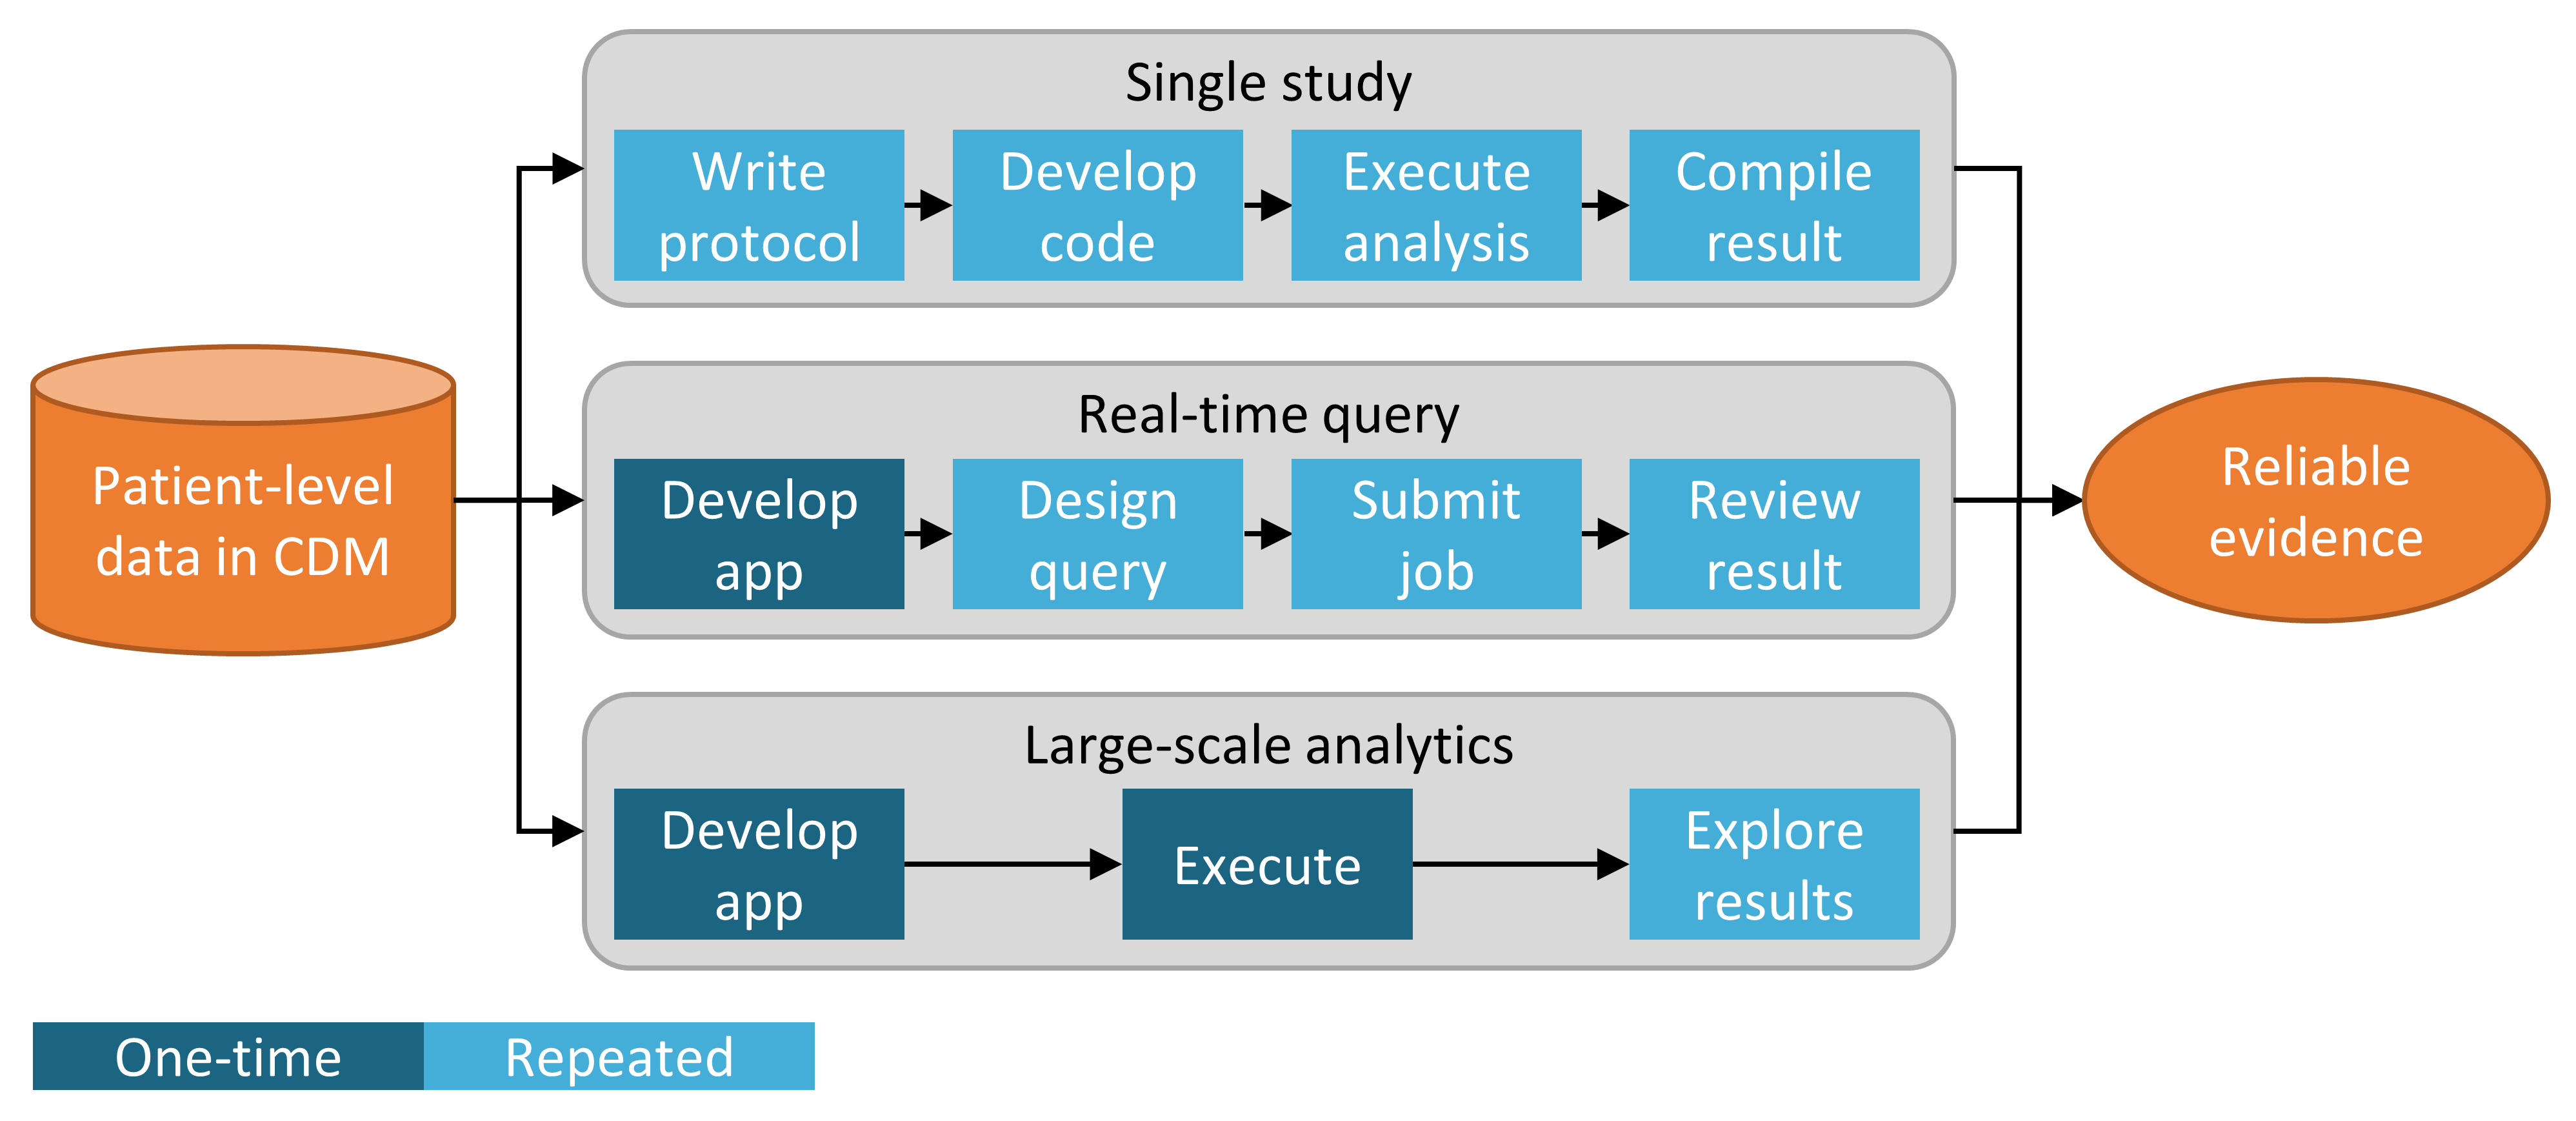
\includegraphics[width=0.9\linewidth]{images/OhdsiAnalyticsTools/strategies} 

}

\caption{Stratégies pour générer des preuves pour des questions (cliniques).}\label{fig:strategies}
\end{figure}

La première stratégie considère chaque analyse comme une étude individuelle unique. L'analyse doit être pré-spécifiée dans un protocole, mise en œuvre sous forme de code, exécutée sur les données, après quoi le résultat peut être compilé et interprété. Pour chaque question, toutes les étapes doivent être répétées. Un exemple de cette analyse est l'étude d'OHDSI sur le risque d'angioedème associé au lévétiracétam par rapport à la phénytoïne. \citep{duke_2017} Ici, un protocole a d'abord été rédigé, le code d'analyse utilisant la Bibliothèque de Méthodes d'OHDSI a été développé et exécuté à travers le réseau OHDSI, et les résultats ont été compilés et disséminés dans une publication de journal.

La deuxième stratégie consiste à développer une application permettant aux utilisateurs de répondre à une classe spécifique de questions en temps réel ou quasi réel. Une fois l'application développée, les utilisateurs peuvent définir des requêtes de manière interactive, les soumettre et visualiser les résultats. Un exemple de cette stratégie est l'outil de définition et de génération de cohortes dans ATLAS. Cet outil permet aux utilisateurs de spécifier des définitions de cohortes de complexité variable et d'exécuter la définition contre une base de données pour voir combien de personnes répondent aux divers critères d'inclusion et d'exclusion.

La troisième stratégie se concentre de manière similaire sur une classe de questions, mais tente ensuite de générer de manière exhaustive toutes les preuves pour les questions de cette classe. Les utilisateurs peuvent ensuite explorer les preuves selon leurs besoins via une variété d'interfaces. Un exemple est l'étude d'OHDSI sur les effets des traitements contre la dépression. \citep{schuemie_2018b} Dans cette étude, tous les traitements contre la dépression sont comparés pour un large ensemble de résultats d'intérêt sur quatre grandes bases de données observationnelles. L'ensemble complet des résultats, incluant 17 718 rapports de risque calibrés empiriquement ainsi que des diagnostics d'études étendus, est disponible dans une application web interactive.\footnote{\url{http://data.ohdsi.org/SystematicEvidence/}}

\section{ATLAS}\label{atlas}

ATLAS est un outil web gratuit et accessible au public, développé par la communauté OHDSI, qui facilite la conception et l'exécution d'analyses sur des données d'observation standardisées au niveau des patients au format CDM. ATLAS est déployé en tant qu'application web en combinaison avec l'OHDSI WebAPI et est généralement hébergé sur Apache Tomcat. La réalisation d'analyses en temps réel nécessite l'accès aux données patient au format CDM et est donc généralement installée derrière le pare-feu d'une organisation. Cependant, il existe également un ATLAS public\footnote{\url{http://www.ohdsi.org/web/atlas}}, et bien que cette instance d'ATLAS n'ait accès qu'à quelques petits jeux de données simulés, elle peut encore être utilisée à de nombreuses fins, y compris les tests et la formation. Il est même possible de définir entièrement une étude d'estimation d'effet ou de prédiction à l'aide de l'instance publique d'ATLAS, et de générer automatiquement le code R pour exécuter l'étude. Ce code peut ensuite être exécuté dans n'importe quel environnement disposant d'un CDM disponible sans avoir besoin d'installer ATLAS et l'API Web. \index{ATLAS}

\begin{figure}

{\centering 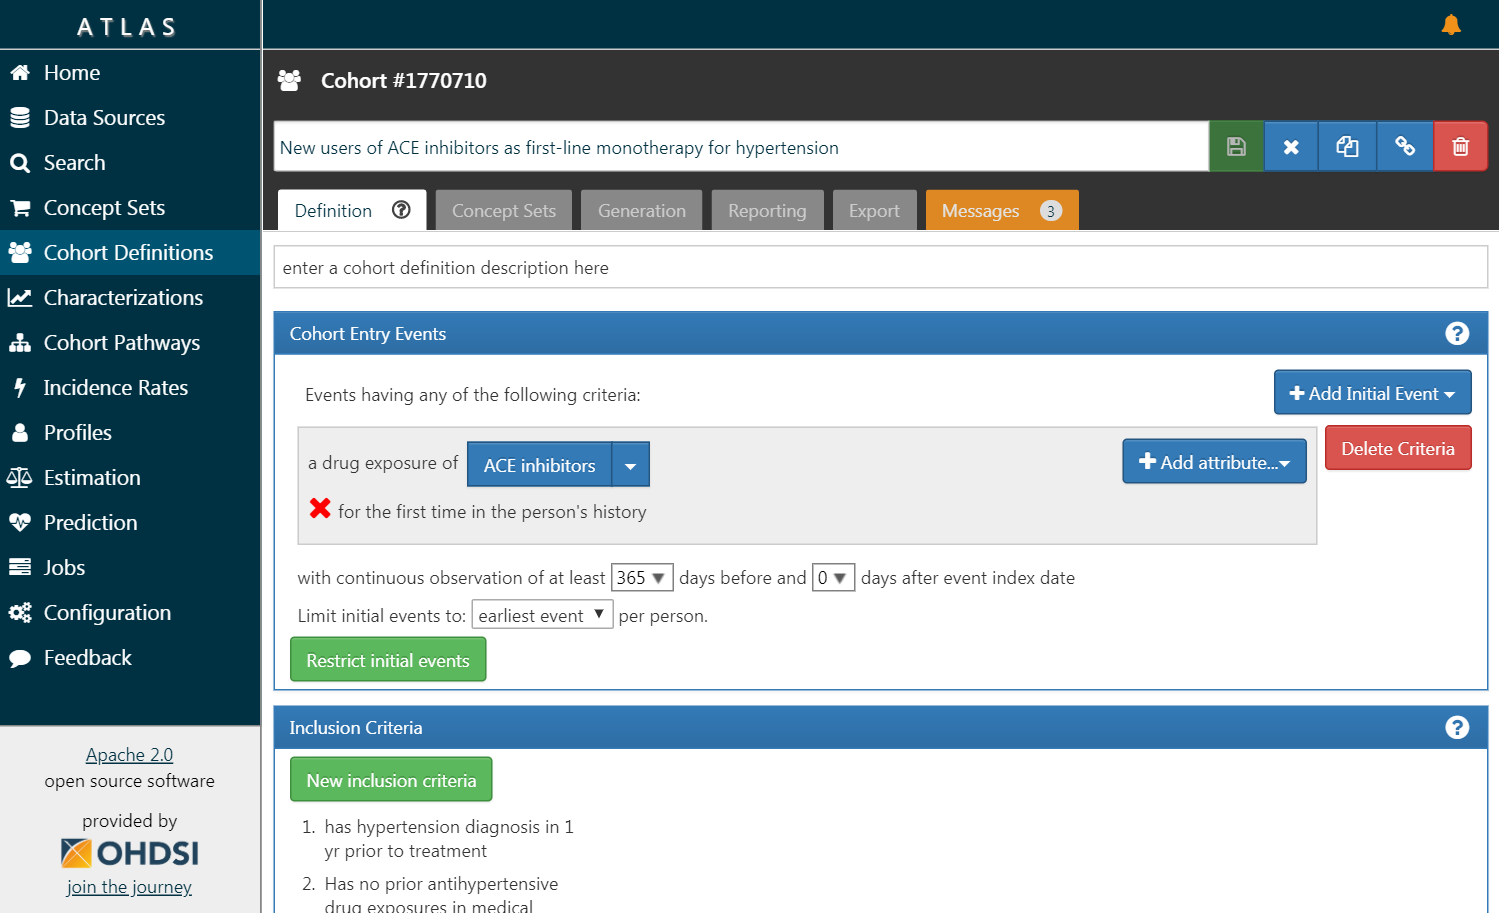
\includegraphics[width=1\linewidth]{images/OhdsiAnalyticsTools/atlas} 

}

\caption{ATLAS user interface.}\label{fig:atlas}
\end{figure}

Une capture d'écran d'ATLAS est fournie à la Figure \ref{fig:atlas}. À gauche se trouve une barre de navigation montrant les différentes fonctions fournies par ATLAS :

\begin{description}
\tightlist
\item[Sources de données \index{ATLAS!Sources de données} \index{Achilles|see {ATLAS!data sources}}]
Les sources de données offrent la possibilité de passer en revue les comptes-rendus descriptifs et standardisés pour chacune des sources de données que vous avez configurées dans votre plateforme Atlas. Cette fonctionnalité utilise la stratégie d'analyse en grande échelle : tous les descriptifs ont été pré-calculés. Les sources de données sont discutées dans le Chapitre \ref{Characterization}.
\item[Recherche de vocabulaire \index{ATLAS!recherche de vocabulaire}]
Atlas permet de rechercher et d'explorer le vocabulaire standardisé OMOP pour comprendre quels concepts existent dans ces vocabulaires et comment appliquer ces concepts dans votre analyse standardisée de vos sources de données. Cette fonctionnalité est discutée dans le Chapitre \ref{StandardizedVocabularies}.
\item[Ensembles de concepts \index{ATLAS!ensembles de concepts}]
Les ensembles de concepts fournissent la capacité de créer des collections d'expressions logiques pouvant être utilisées pour identifier un ensemble de concepts à utiliser tout au long de vos analyses standardisées. Les ensembles de concepts offrent plus de sophistication qu'une simple liste de codes ou de valeurs. Un ensemble de concepts est composé de plusieurs concepts du vocabulaire standardisé en combinaison avec des indicateurs logiques permettant à un utilisateur de préciser qu'il souhaite inclure ou exclure des concepts liés à la hiérarchie du vocabulaire. La recherche dans le vocabulaire, l'identification de l'ensemble des concepts et la spécification de la logique à utiliser pour résoudre un ensemble de concepts offrent un mécanisme puissant pour définir le langage médical souvent obscur utilisé dans les plans d'analyse. Ces ensembles de concepts peuvent être enregistrés dans ATLAS et être ensuite utilisés tout au long de votre analyse comme partie des définitions de cohortes ou des spécifications d'analyse.
\item[Définitions de cohortes \index{ATLAS!définitions de cohortes}]
Les définitions de cohortes permettent de construire un ensemble de personnes qui satisfont un ou plusieurs critères pendant une durée de temps et ces cohortes peuvent ensuite servir de base aux saisies pour l'ensemble de vos analyses ultérieures. Cette fonctionnalité est discutée dans le Chapitre \ref{Cohorts}.
\item[Caractérisations \index{ATLAS!caractérisations des cohortes}]
Les caractérisations sont une capacité analytique qui vous permet d'examiner une ou plusieurs cohortes que vous avez définies et de résumer les caractéristiques de ces populations de patients. Cette fonctionnalité utilise la stratégie de requête en temps réel et est discutée dans le Chapitre \ref{Characterization}.
\item[Trajectoires de cohortes \index{ATLAS!trajectoires de cohortes}]
Les trajectoires de cohortes sont un outil analytique qui vous permet d'examiner la séquence des événements cliniques qui se produisent au sein d'une ou plusieurs populations. Cette fonctionnalité utilise la stratégie de requête en temps réel et est discutée dans le Chapitre \ref{Characterization}.
\item[Taux d'incidence \index{ATLAS!taux d'incidence}]
Les taux d'incidence sont un outil qui vous permet d'estimer l'incidence de résultats au sein des populations cibles d'intérêt. Cette fonctionnalité utilise la stratégie de requête en temps réel et est discutée dans le Chapitre \ref{Characterization}.
\item[Profils \index{ATLAS!profils}]
Les profils sont un outil qui vous permet d'explorer les données d'observation longitudinales d'un patient individuel pour résumer ce qui se passe chez un individu donné. Cette fonctionnalité utilise la stratégie de requête en temps réel.
\item[Estimation au niveau de la population \index{ATLAS!estimation au niveau de la population}]
L'estimation est une capacité qui vous permet de définir une étude d'estimation des effets au niveau de la population en utilisant un modèle de cohortes comparatives dans lequel des comparaisons entre une ou plusieurs cohortes cibles et comparateurs peuvent être explorées pour une série de résultats. Cette fonctionnalité peut être dite pour implémenter la stratégie de requête en temps réel, puisque aucune programmation n'est requise, et est discutée dans le Chapitre \ref{PopulationLevelEstimation}.
\item[Prédiction au niveau des patients \index{ATLAS!prédiction au niveau des patients}]
La prédiction est une capacité qui vous permet d'appliquer des algorithmes d'apprentissage automatique pour mener des analyses de prédiction au niveau des patients dans lesquelles vous pouvez prédire un résultat dans n'importe quelle exposition cible donnée. Cette fonctionnalité peut être dite pour implémenter la stratégie de requête en temps réel, puisque aucune programmation n'est requise, et est discutée dans le Chapitre \ref{PatientLevelPrediction}.
\item[Tâches \index{ATLAS!tâches}]
Sélectionnez l'élément de menu Tâches pour explorer l'état des processus en cours d'exécution via le WebAPI. Les tâches sont souvent des processus de longue durée tels que la génération d'une cohorte ou le calcul des rapports de caractérisation de cohorte.
\item[Configuration \index{ATLAS!configuration}]
Sélectionnez l'élément de menu Configuration pour consulter les sources de données qui ont été configurées dans la section de configuration de source.
\item[Retour d'information \index{ATLAS!retour d'information}]
Le lien Retour d'information vous mènera au journal des problèmes d'Atlas afin que vous puissiez enregistrer un nouveau problème ou rechercher parmi les problèmes existants. Si vous avez des idées pour de nouvelles fonctionnalités ou améliorations, c'est également un endroit pour les noter pour la communauté de développement.
\end{description}

\subsection{Sécurité}\label{suxe9curituxe9}

ATLAS et le WebAPI fournissent un modèle de sécurité granulaire pour contrôler l'accès aux fonctionnalités ou aux sources de données au sein de la plateforme globale. Le système de sécurité est construit en utilisant la bibliothèque Apache Shiro. Des informations supplémentaires sur le système de sécurité peuvent être trouvées dans le wiki en ligne sur la sécurité de WebAPI.\footnote{\url{https://github.com/OHDSI/WebAPI/wiki/Security-Configuration}} \index{ATLAS!sécurité}

\subsection{Documentation}\label{documentation}

La documentation pour ATLAS peut être trouvée en ligne dans le wiki du dépôt GitHub d'ATLAS.\footnote{\url{https://github.com/OHDSI/ATLAS/wiki}} Ce wiki comprend des informations sur les différentes fonctionnalités de l'application ainsi que des liens vers des tutoriels vidéo en ligne. \index{ATLAS!documentation}

\subsection{Comment installer}\label{comment-installer}

L'installation d'ATLAS se fait en combinaison avec le WebAPI d'OHDSI. Les guides d'installation pour chaque composant sont disponibles en ligne dans le Guide de configuration du dépôt GitHub d'ATLAS\footnote{\url{https://github.com/OHDSI/Atlas/wiki/Atlas-Setup-Guide}} et le Guide d'installation du dépôt GitHub de WebAPI.\footnote{\url{https://github.com/OHDSI/WebAPI/wiki/WebAPI-Installation-Guide}} \index{ATLAS!installation}

\section{Bibliothèque de Méthodes}\label{bibliothuxe8que-de-muxe9thodes}

La \href{https://ohdsi.github.io/MethodsLibrary/}{Bibliothèque de Méthodes OHDSI} est la collection de packages R open source présentés dans la Figure \ref{fig:methodsLibrary}. \index{bibliothèque de méthodes}

\begin{figure}

{\centering 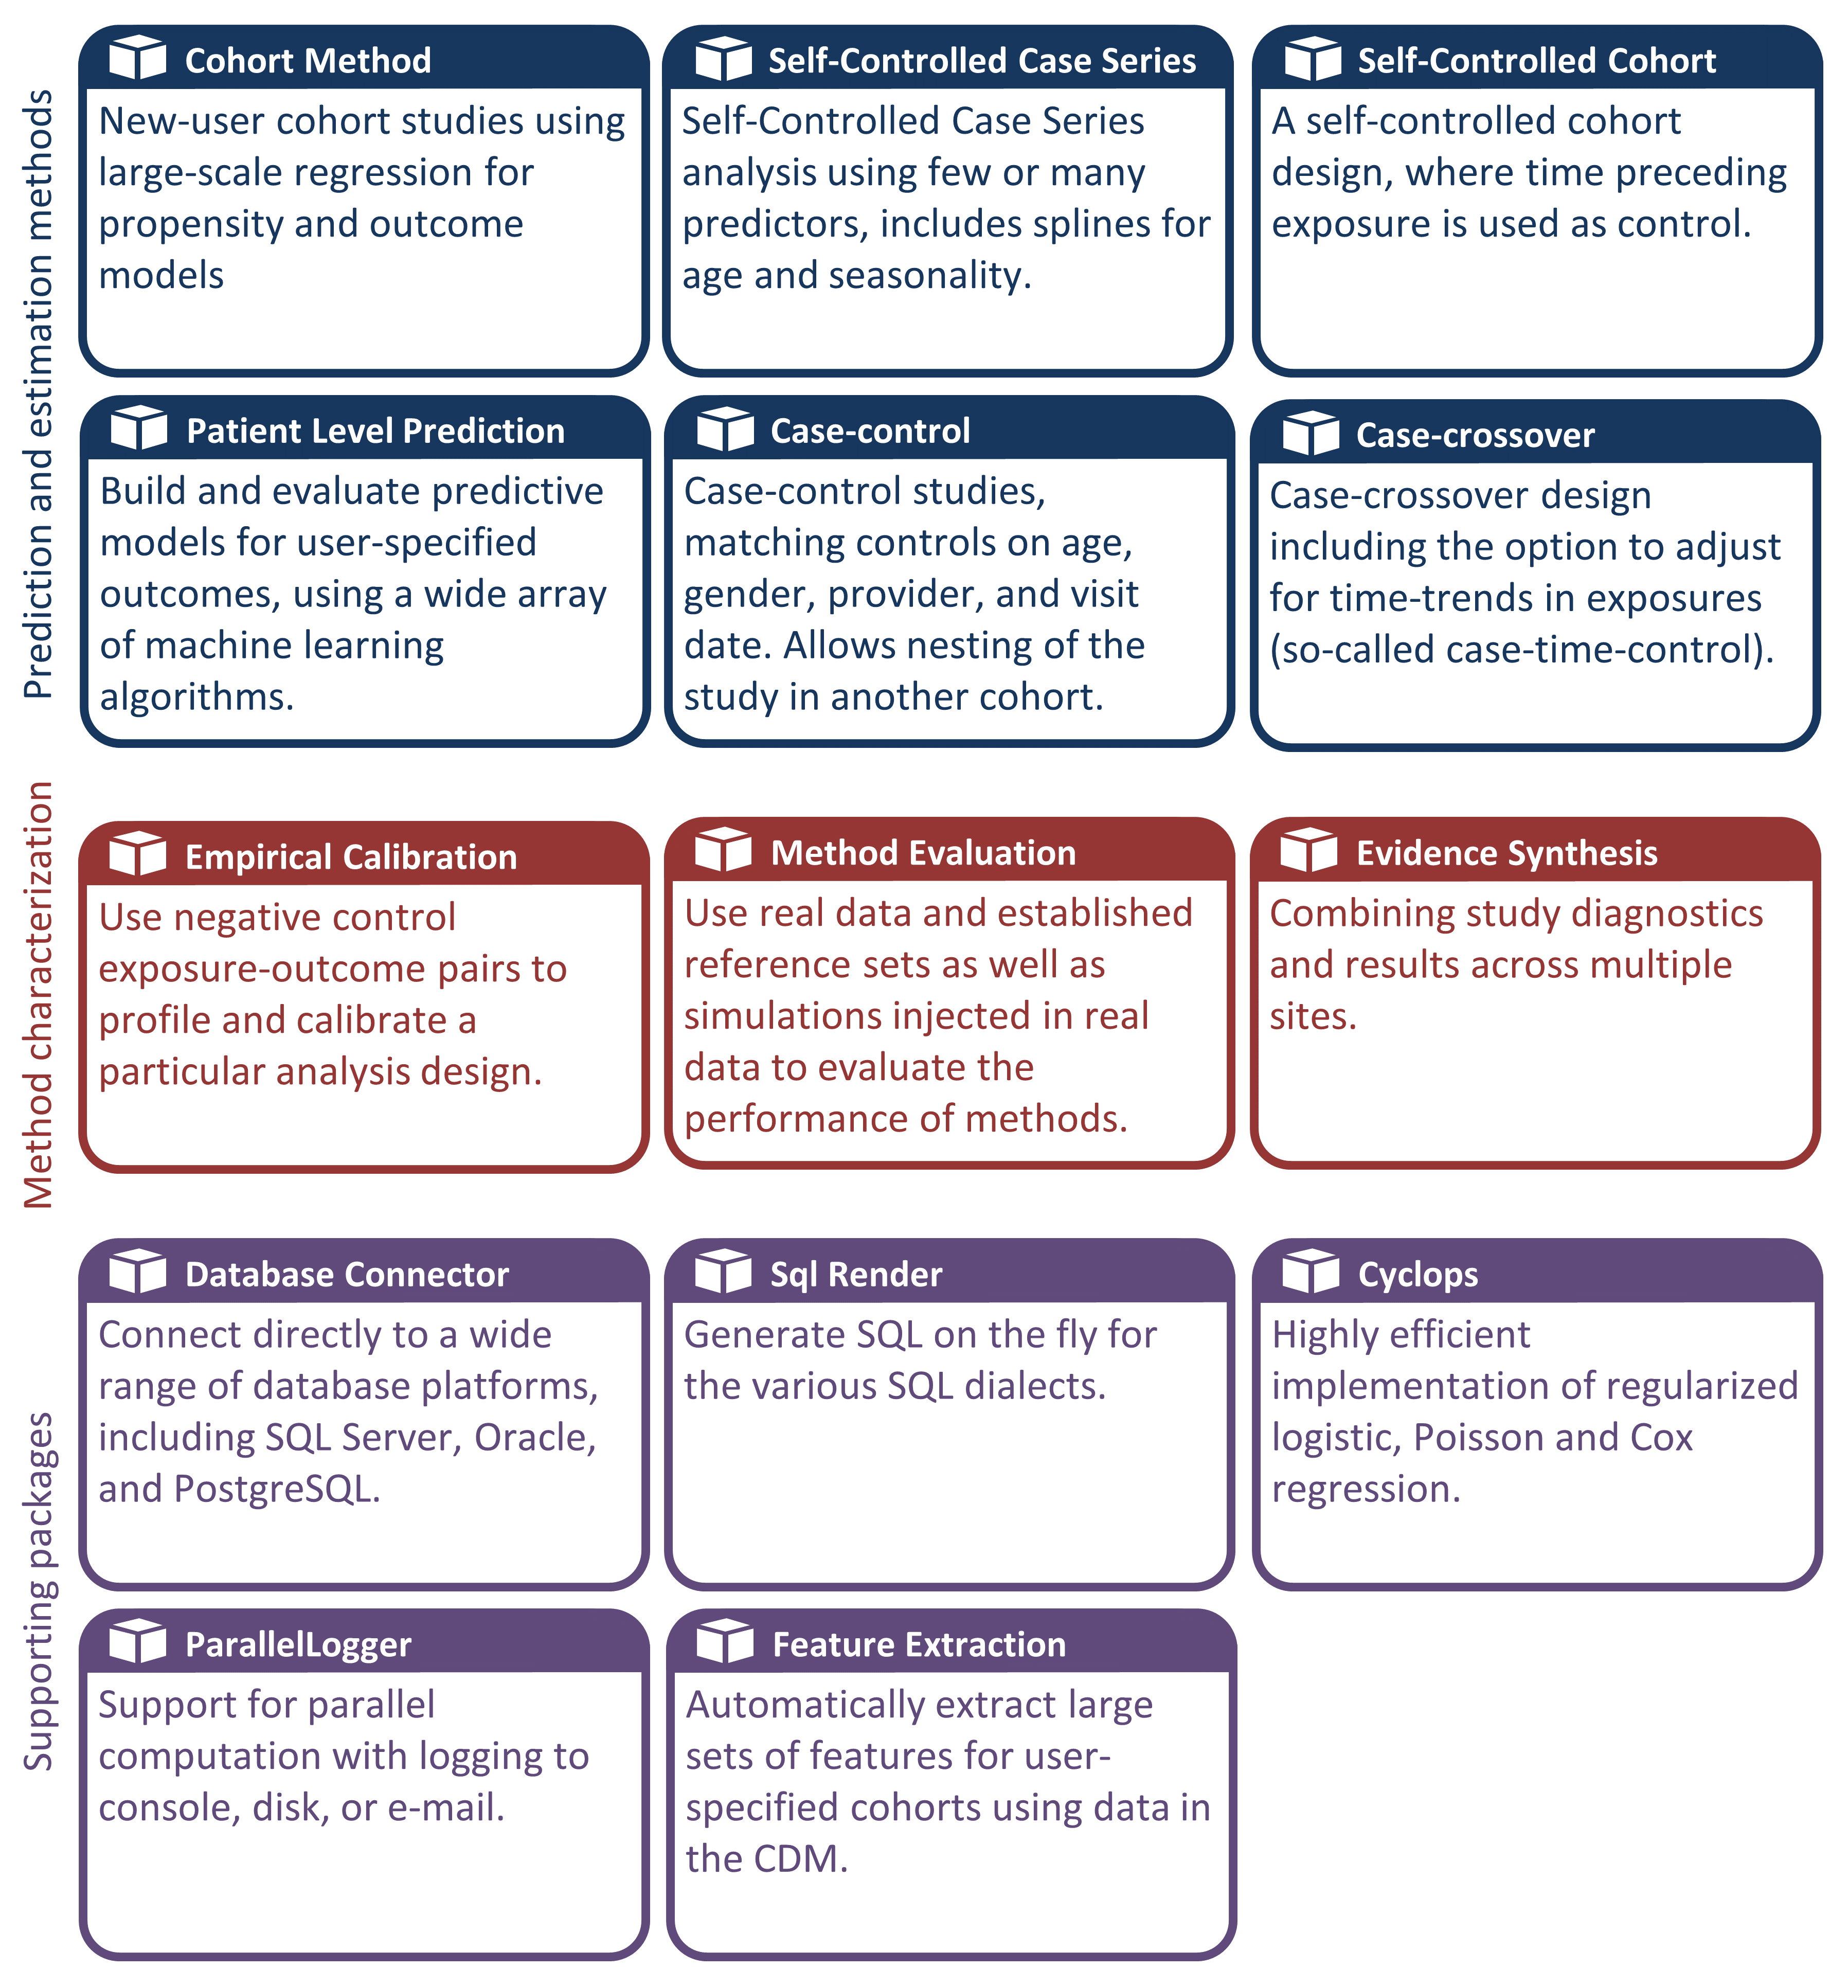
\includegraphics[width=1\linewidth]{images/OhdsiAnalyticsTools/methodsLibrary} 

}

\caption{Packages in the OHDSI Methods Library.}\label{fig:methodsLibrary}
\end{figure}

Les packages offrent des fonctions R qui, ensemble, peuvent être utilisées pour réaliser une étude observationnelle complète, à partir des données dans le CDM, et aboutissant à des estimations et des statistiques, figures et tableaux de soutien. Les packages interagissent directement avec les données observationnelles dans le CDM, et peuvent être utilisés simplement pour fournir une compatibilité multiplateforme pour des analyses complètement personnalisées comme décrit au Chapitre \ref{SqlAndR}, ou peuvent fournir des analyses standardisées avancées pour la caractérisation de la population (Chapitre \ref{Characterization}), l'estimation de l'effet au niveau de la population (Chapitre \ref{PopulationLevelEstimation}), et la prédiction au niveau des patients (Chapitre \ref{PatientLevelPrediction}). La Bibliothèque de Méthodes soutient les meilleures pratiques pour l'utilisation des données observationnelles et la conception des études observationnelles telles qu'enseignées par des recherches passées et en cours, telles que la transparence, la reproductibilité, ainsi que la mesure des caractéristiques de fonctionnement des méthodes dans un contexte particulier et l'étalonnage empirique des estimations produites par les méthodes.

La Bibliothèque de Méthodes a déjà été utilisée dans de nombreuses études cliniques publiées \citep{boland_2017, duke_2017, ramcharran_2017, weinstein_2017, wang_2017, ryan_2017, ryan_2018, vashisht_2018, yuan_2018, johnston_2019}, ainsi que des études méthodologiques. \citep{schuemie_2014, schuemie_2016, reps2018, tian_2018, schuemie_2018, schuemie_2018b, reps_2019} La validité des implémentations des méthodes dans la bibliothèque de méthodes est décrite dans le Chapitre \ref{SoftwareValidity}.

\subsection{Support pour les Analyses à Grande Échelle}\label{support-pour-les-analyses-uxe0-grande-uxe9chelle}

Une caractéristique clé incorporée dans tous les packages est la capacité de réaliser efficacement de nombreuses analyses. Par exemple, lors de la réalisation d'une estimation au niveau de la population, le package CohortMethod permet de calculer des estimations de la taille de l'effet pour de nombreuses expositions et résultats, en utilisant divers paramètres d'analyse, et le package choisira automatiquement le meilleur moyen de calculer tous les ensembles de données intermédiaires et finaux nécessaires. Les étapes qui peuvent être réutilisées, telles que l'extraction des covariables ou l'ajustement d'un modèle de propension utilisé pour une paire cible-comparateur mais de multiples résultats, ne seront exécutées qu'une fois. Lorsque cela est possible, les calculs se feront en parallèle pour maximiser l'utilisation des ressources informatiques.

Cette efficacité informatique permet des analyses à grande échelle, répondant à de nombreuses questions à la fois, et est également essentielle pour inclure des hypothèses de contrôle (par exemple, des contrôles négatifs) pour mesurer les caractéristiques de fonctionnement de nos méthodes et effectuer un étalonnage empirique comme décrit au Chapitre \ref{MethodValidity}. \index{hypothèses de contrôle}

\subsection{Support pour les Big Data}\label{BigDataSupport}

La Bibliothèque de Méthodes est également conçue pour fonctionner sur des bases de données très volumineuses et être capable d'effectuer des calculs impliquant de grandes quantités de données. Cela est réalisé de trois manières~:

\begin{enumerate}
\def\labelenumi{\arabic{enumi}.}
\tightlist
\item
  La plupart des manipulations de données sont effectuées sur le serveur de base de données. Une analyse ne nécessite généralement qu'une petite fraction de l'ensemble des données dans la base de données, et la Bibliothèque de Méthodes, via les packages SqlRender et DatabaseConnector, permet d'effectuer des opérations avancées sur le serveur pour prétraiter et extraire les données pertinentes.
\item
  Les grands objets de données locaux sont stockés de manière économe en mémoire. Pour les données téléchargées sur la machine locale, la Bibliothèque de Méthodes utilise le package \href{https://cran.r-project.org/web/packages/ff}{ff} pour stocker et travailler avec de grands objets de données. Cela nous permet de travailler avec des données bien plus importantes que ce qui tiendrait en mémoire.
\item
  L'informatique haute performance est appliquée là où c'est nécessaire. Par exemple, le package \href{https://ohdsi.github.io/Cyclops/}{Cyclops} implémente un moteur de régression extrêmement efficace qui est utilisé dans toute la Bibliothèque de Méthodes pour effectuer des régressions à grande échelle (grand nombre de variables, grand nombre d'observations) qui seraient autrement impossibles à ajuster.
\end{enumerate}

\subsection{Documentation}\label{documentation-1}

R fournit une manière standard de documenter les packages. Chaque package possède un \emph{manuel de package} qui documente chaque fonction et ensemble de données contenu dans le package. Tous les manuels de package sont disponibles en ligne via le site de la Bibliothèque de Méthodes\footnote{\url{https://ohdsi.github.io/MethodsLibrary}}, via les dépôts GitHub des packages, et pour les packages disponibles via CRAN, ils peuvent être trouvés sur CRAN. De plus, depuis R, le manuel de package peut être consulté en utilisant le point d'interrogation. Par exemple, après avoir chargé le package DatabaseConnector, taper la commande \texttt{?connect} permet d'accéder à la documentation de la fonction ``connect''.

En plus du manuel de package, de nombreux packages fournissent des \emph{vignettes}. Les vignettes sont des documentations détaillées qui décrivent comment un package peut être utilisé pour réaliser certaines tâches. Par exemple, une vignette\footnote{\url{https://ohdsi.github.io/CohortMethod/articles/MultipleAnalyses.html}} décrit comment réaliser plusieurs analyses de manière efficace en utilisant le package CohortMethod. Les vignettes peuvent également être trouvées via le site de la Bibliothèque de Méthodes, via les dépôts GitHub des packages, et pour les packages disponibles via CRAN, elles peuvent être trouvées sur CRAN. \index{vignette}

\subsection{Exigences Systémiques}\label{exigences-systuxe9miques}

Deux environnements informatiques sont pertinents lorsqu'on discute des exigences systémiques~: Le serveur de base de données et la station de travail analytique. \index{exigences systémiques}

Le serveur de base de données doit contenir les données observationnelles de santé au format CDM. La Bibliothèque de Méthodes prend en charge une large gamme de systèmes de gestion de base de données, y compris les systèmes de base de données traditionnels (PostgreSQL, Microsoft SQL Server et Oracle), les entrepôts de données parallèles (Microsoft APS, IBM Netezza et Amazon Redshift), ainsi que les plateformes de Big Data (Hadoop via Impala et Google BigQuery).

La station de travail analytique est l'endroit où la Bibliothèque de Méthodes est installée et exécutée. Cela peut être une machine locale, comme l'ordinateur portable de quelqu'un, ou un serveur distant exécutant RStudio Server. Dans tous les cas, les exigences sont que R soit installé, de préférence avec RStudio. La Bibliothèque de Méthodes nécessite également que Java soit installé. La station de travail analytique doit également pouvoir se connecter au serveur de base de données, en particulier, tout pare-feu entre eux doit avoir les ports d'accès au serveur de base de données ouverts sur la station de travail. Certaines analyses peuvent être intensives en calcul, donc avoir plusieurs cœurs de traitement et une mémoire ample peut aider à accélérer les analyses. Nous recommandons d'avoir au moins quatre cœurs et 16 gigaoctets de mémoire.

\subsection{Comment Installer}\label{installR}

Voici les étapes pour installer l'environnement requis pour exécuter les packages R d'OHDSI. Quatre éléments doivent être installés~: \index{R!installation}

\begin{enumerate}
\def\labelenumi{\arabic{enumi}.}
\tightlist
\item
  \textbf{R} est un environnement de calcul statistique. Il est livré avec une interface utilisateur de base qui est principalement une interface en ligne de commande.
\item
  \textbf{Rtools} est un ensemble de programmes requis sous Windows pour construire des packages R à partir du code source.
\item
  \textbf{RStudio} est un IDE (environnement de développement intégré) qui facilite l'utilisation de R. Il inclut un éditeur de code, des outils de débogage et de visualisation. Veuillez l'utiliser pour obtenir une expérience R agréable.
\item
  \textbf{Java} est un environnement de calcul nécessaire pour exécuter certains composants dans les packages R OHDSI, par exemple ceux nécessaires pour se connecter à une base de données.
\end{enumerate}

Ci-dessous, nous décrivons comment installer chacun de ces éléments dans un environnement Windows.

\begin{rmdimportant}
Sous Windows, R et Java existent en versions 32 bits et 64 bits. Si vous installez R dans les deux architectures, vous \textbf{devez} également installer Java dans les deux architectures. Il est recommandé de n'installer que la version 64 bits de R.
\end{rmdimportant}

\subsubsection*{Installer R}\label{installer-r}
\addcontentsline{toc}{subsubsection}{Installer R}

\begin{enumerate}
\def\labelenumi{\arabic{enumi}.}
\tightlist
\item
  Aller sur \url{https://cran.r-project.org/}, cliquez sur ``Download R for Windows'', puis ``base'', puis cliquez sur le lien de téléchargement indiqué dans la Figure \ref{fig:downloadR}.
\end{enumerate}

\begin{figure}

{\centering 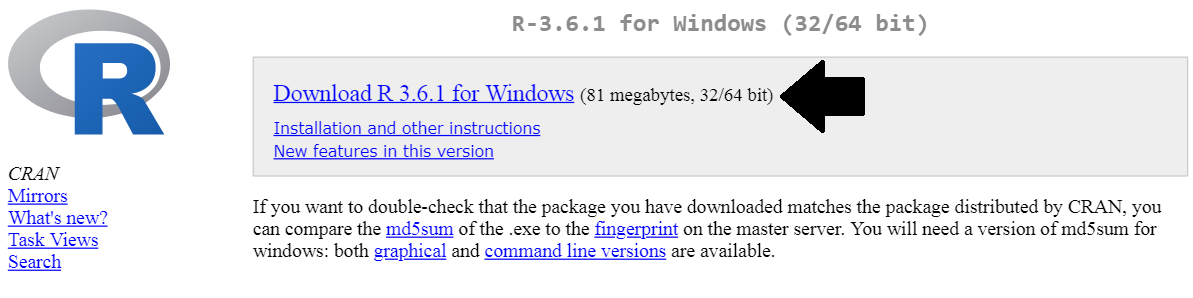
\includegraphics[width=1\linewidth]{images/OhdsiAnalyticsTools/downloadR} 

}

\caption{Downloading R from CRAN.}\label{fig:downloadR}
\end{figure}

\begin{enumerate}
\def\labelenumi{\arabic{enumi}.}
\setcounter{enumi}{1}
\tightlist
\item
  Après avoir terminé le téléchargement, exécutez le programme d'installation. Utilisez les options par défaut partout, à deux exceptions près~: Premièrement, il est préférable de ne pas installer dans les fichiers de programme. Au lieu de cela, faites simplement de R un sous-dossier de votre lecteur C comme montré dans la Figure \ref{fig:rDestination}. Deuxièmement, pour éviter les problèmes dus aux différences d'architectures entre R et Java, désactivez l'architecture 32 bits comme montré dans la Figure \ref{fig:no32Bits}.
\end{enumerate}

\begin{figure}

{\centering 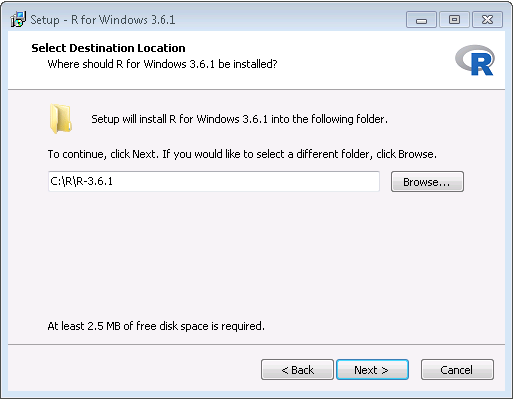
\includegraphics[width=0.8\linewidth]{images/OhdsiAnalyticsTools/rDestination} 

}

\caption{Settings the destination folder for R.}\label{fig:rDestination}
\end{figure}

\begin{figure}

{\centering 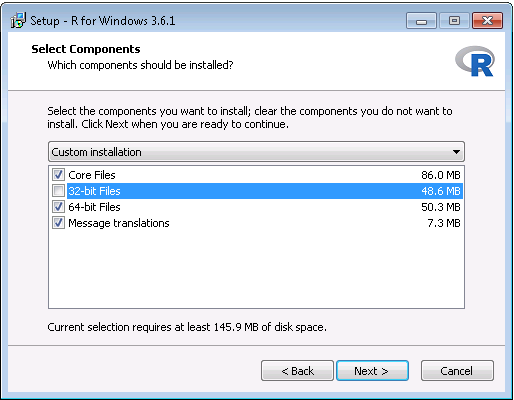
\includegraphics[width=0.8\linewidth]{images/OhdsiAnalyticsTools/no32Bits} 

}

\caption{Disabling the 32-bit version of R.}\label{fig:no32Bits}
\end{figure}

Une fois terminé, vous devriez pouvoir sélectionner R depuis votre menu Démarrer.

\subsubsection*{Installer Rtools}\label{installer-rtools}
\addcontentsline{toc}{subsubsection}{Installer Rtools}

\begin{enumerate}
\def\labelenumi{\arabic{enumi}.}
\item
  Aller sur \url{https://cran.r-project.org/}, cliquez sur ``Download R for Windows'', puis ``Rtools'', et sélectionnez la toute dernière version de Rtools à télécharger.
\item
  Après avoir terminé le téléchargement, exécutez le programme d'installation. Sélectionnez les options par défaut partout.
\end{enumerate}

\subsubsection*{Installer RStudio}\label{installer-rstudio}
\addcontentsline{toc}{subsubsection}{Installer RStudio}

\begin{enumerate}
\def\labelenumi{\arabic{enumi}.}
\tightlist
\item
  Aller sur \url{https://www.rstudio.com/}, sélectionnez ``Download RStudio'' (ou le bouton ``Download'' sous ``RStudio''), optez pour la version gratuite, et téléchargez le programme d'installation pour Windows comme montré dans la Figure \ref{fig:downloadRStudio}.
\end{enumerate}

\begin{figure}

{\centering 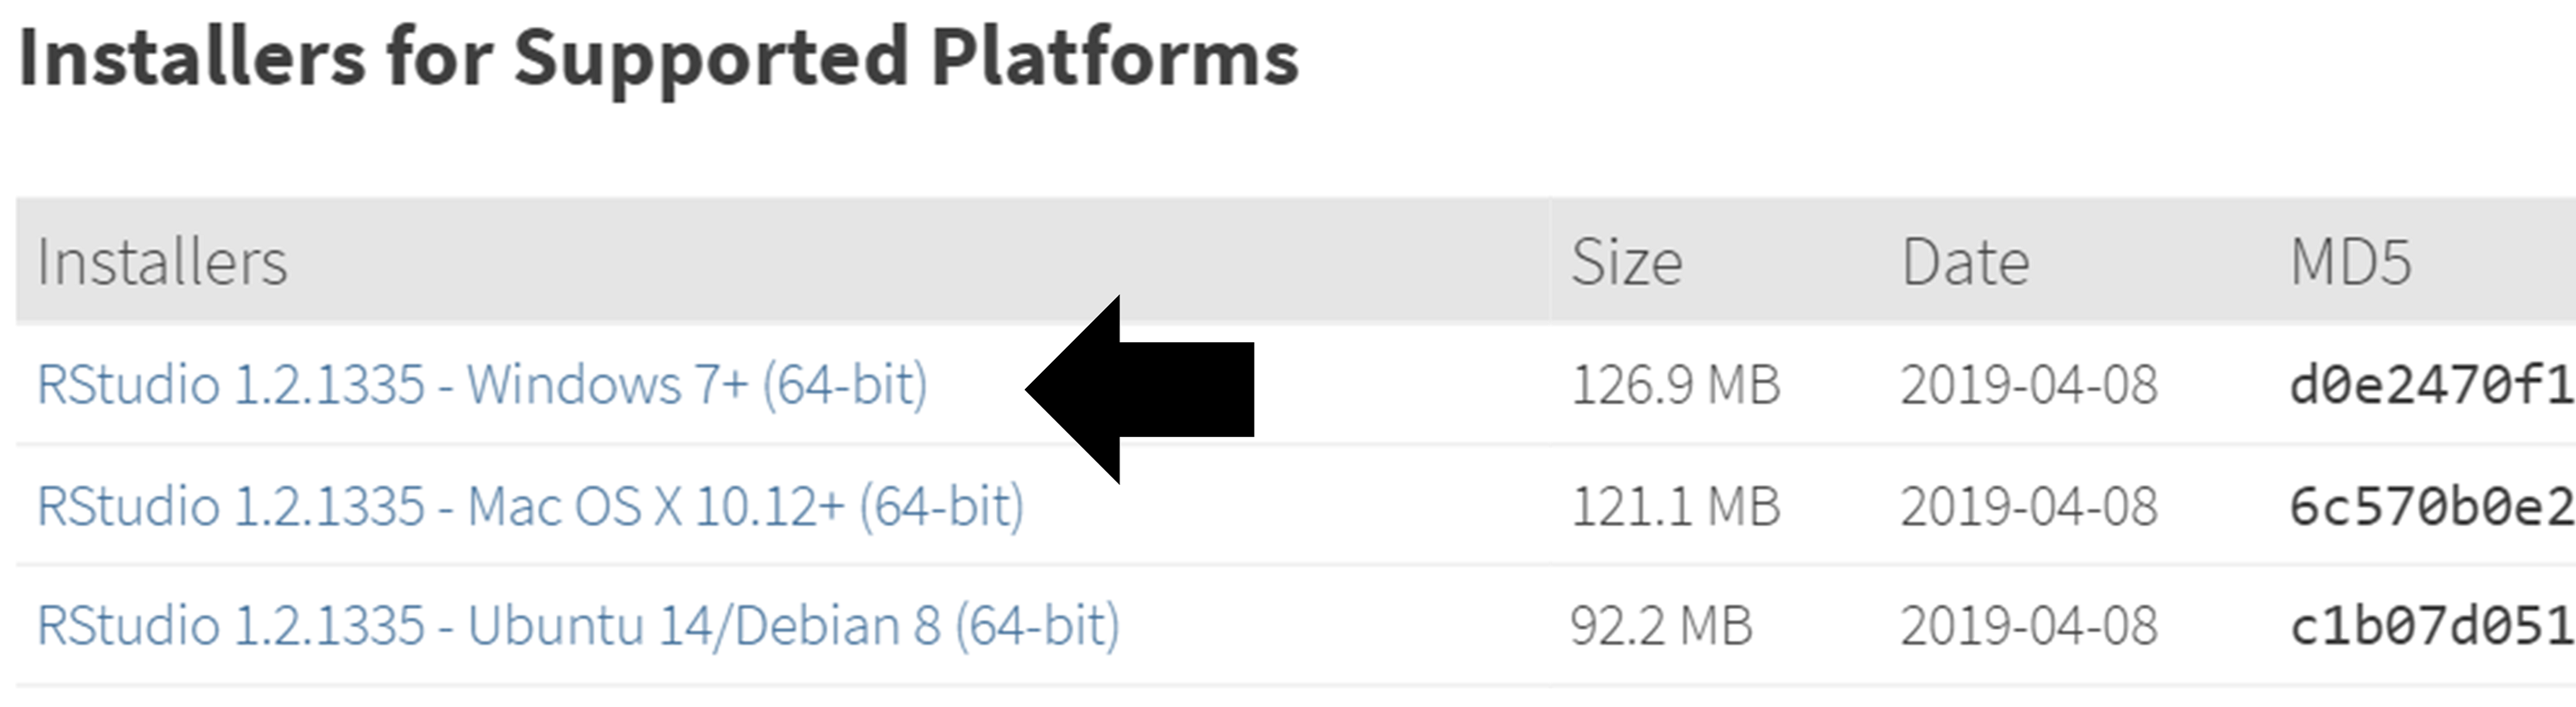
\includegraphics[width=1\linewidth]{images/OhdsiAnalyticsTools/downloadRStudio} 

}

\caption{Downloading RStudio.}\label{fig:downloadRStudio}
\end{figure}

\begin{enumerate}
\def\labelenumi{\arabic{enumi}.}
\setcounter{enumi}{1}
\tightlist
\item
  Après avoir téléchargé, démarrer le programme d'installation, et utilisez les options par défaut partout.
\end{enumerate}

\subsubsection*{Installer Java}\label{installer-java}
\addcontentsline{toc}{subsubsection}{Installer Java}

\begin{enumerate}
\def\labelenumi{\arabic{enumi}.}
\tightlist
\item
  Aller sur \url{https://java.com/en/download/manual.jsp}, et sélectionnez le programme d'installation Windows 64 bits comme montré dans la Figure \ref{fig:downloadJava}. Si vous avez également installé la version 32 bits de R, vous \emph{devez} également installer l'autre version (32 bits) de Java.
\end{enumerate}

\begin{figure}

{\centering 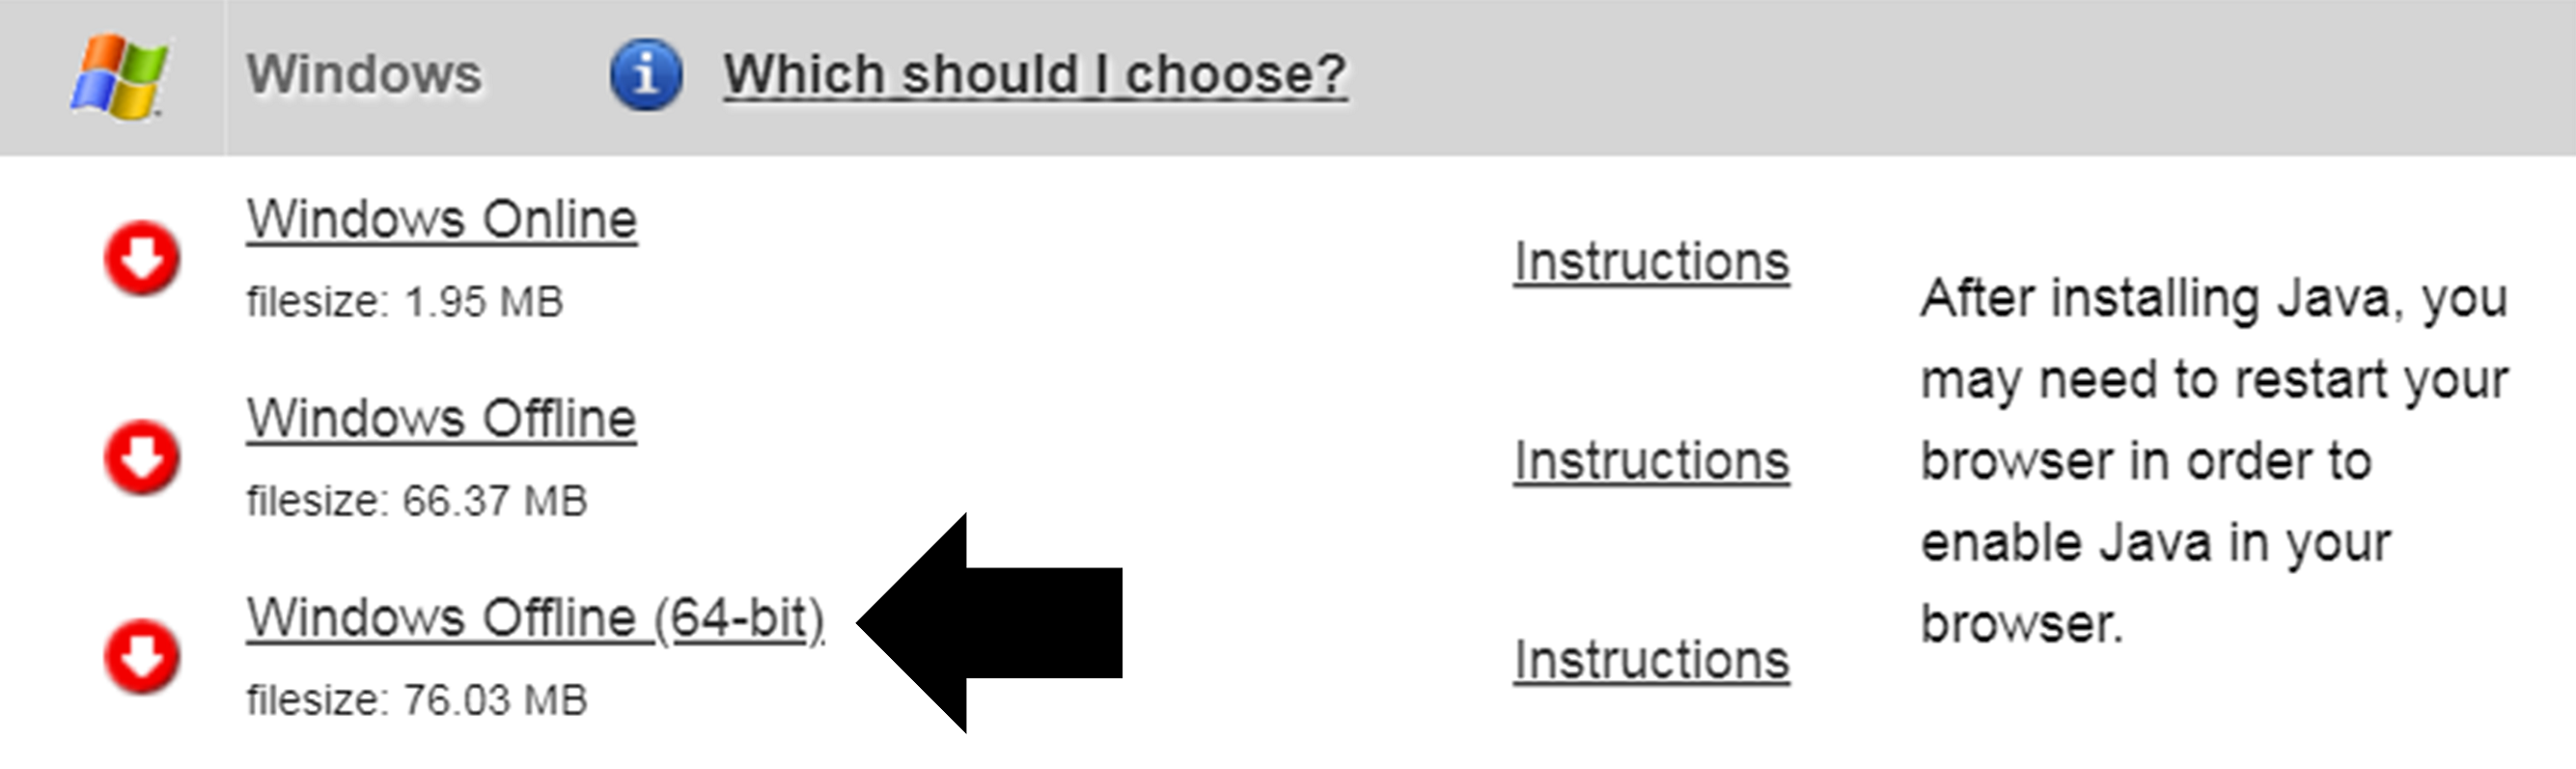
\includegraphics[width=1\linewidth]{images/OhdsiAnalyticsTools/downloadJava} 

}

\caption{Downloading Java.}\label{fig:downloadJava}
\end{figure}

\begin{enumerate}
\def\labelenumi{\arabic{enumi}.}
\setcounter{enumi}{1}
\tightlist
\item
  Après avoir téléchargé, exécutez simplement le programme d'installation.
\end{enumerate}

\subsubsection*{Vérifier l'Installation}\label{vuxe9rifier-linstallation}
\addcontentsline{toc}{subsubsection}{Vérifier l'Installation}

Vous devriez maintenant être prêt à partir, mais nous devrions vérifier. Démarrez RStudio et tapez

\begin{Shaded}
\begin{Highlighting}[]
\FunctionTok{install.packages}\NormalTok{(}\StringTok{"SqlRender"}\NormalTok{)}
\FunctionTok{library}\NormalTok{(SqlRender)}
\FunctionTok{translate}\NormalTok{(}\StringTok{"SELECT TOP 10 * FROM person;"}\NormalTok{, }\StringTok{"postgresql"}\NormalTok{)}
\end{Highlighting}
\end{Shaded}

\begin{verbatim}
## [1] "SELECT  * FROM person LIMIT 10;"
## attr(,"sqlDialect")
## [1] "postgresql"
\end{verbatim}

Cette fonction utilise Java, donc si tout se passe bien, nous savons que R et Java ont été installés correctement~!

Un autre test consiste à voir si les packages source peuvent être construits. Exécutez le code R suivant pour installer le package \texttt{CohortMethod} à partir du dépôt GitHub d'OHDSI :

\begin{Shaded}
\begin{Highlighting}[]
\FunctionTok{install.packages}\NormalTok{(}\StringTok{"drat"}\NormalTok{)}
\NormalTok{drat}\SpecialCharTok{::}\FunctionTok{addRepo}\NormalTok{(}\StringTok{"OHDSI"}\NormalTok{)}
\FunctionTok{install.packages}\NormalTok{(}\StringTok{"CohortMethod"}\NormalTok{)}
\end{Highlighting}
\end{Shaded}

\section{Stratégies de déploiement}\label{stratuxe9gies-de-duxe9ploiement}

Déployer l'ensemble de la pile d'outils OHDSI, y compris ATLAS et la Méthode Bibliothèque, dans une organisation est une tâche ardue. Il y a de nombreux composants avec des dépendances qui doivent être considérées, et des configurations à définir. Pour cette raison, deux initiatives ont développé des stratégies de déploiement intégrées qui permettent d'installer l'ensemble de la pile comme un seul package, en utilisant certaines formes de virtualisation : Broadsea et Amazon Web Services (AWS). \index{tools deployment}

\subsection{Broadsea}\label{broadsea}

Broadsea\footnote{\url{https://github.com/OHDSI/Broadsea}} utilise la technologie des conteneurs Docker.\footnote{\url{https://www.docker.com/}} Les outils OHDSI sont emballés avec des dépendances dans un seul fichier binaire portable appelé une Image Docker. Cette image peut ensuite être exécutée sur un service de moteur Docker, créant une machine virtuelle avec tout le logiciel installé et prêt à fonctionner. Les moteurs Docker sont disponibles pour la plupart des systèmes d'exploitation, y compris Microsoft Windows, MacOS et Linux. L'image Docker Broadsea contient les principaux outils OHDSI, y compris la Méthode Bibliothèque et ATLAS. \index{tools deployment!Broadsea}

\subsection{Amazon AWS}\label{amazon-aws}

Amazon a préparé deux environnements qui peuvent être instanciés dans l'environnement de cloud computing AWS d'un simple clic : OHDSI-in-a-Box\footnote{\url{https://github.com/OHDSI/OHDSI-in-a-Box}} et OHDSIonAWS.\footnote{\url{https://github.com/OHDSI/OHDSIonAWS}} \index{tools deployment!Amazon AWS}

OHDSI-in-a-Box est spécifiquement créé comme un environnement d'apprentissage, et est utilisé dans la plupart des tutoriels fournis par la communauté OHDSI. Il comprend de nombreux outils OHDSI, ensembles de données échantillons, RStudio et d'autres logiciels de support dans une seule machine virtuelle Windows à faible coût. Une base de données PostgreSQL est utilisée pour stocker le CDM et également pour stocker les résultats intermédiaires d'ATLAS. Les outils de mappage des données CDM OMOP et ETL sont également inclus dans OHDSI-in-a-Box. L'architecture de OHDSI-in-a-Box est décrite dans la Figure \ref{fig:ohdsiinaboxDiagram}.

\begin{figure}

{\centering 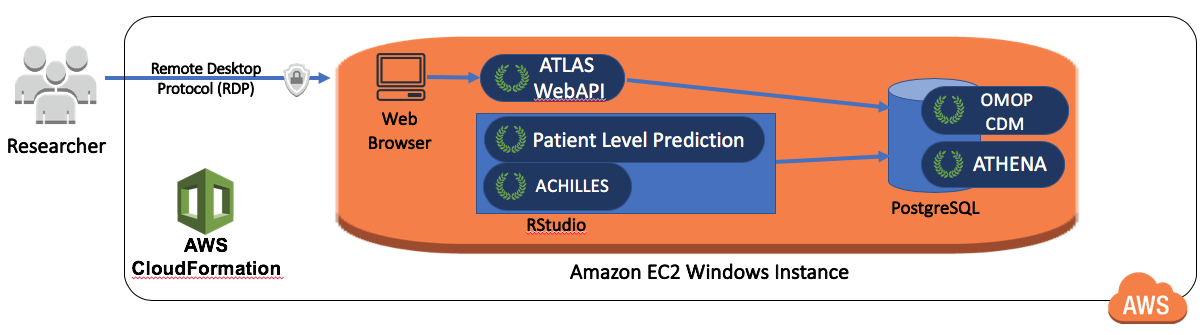
\includegraphics[width=1\linewidth]{images/OhdsiAnalyticsTools/OHDSI-in-a-BoxDiagram} 

}

\caption{The Amazon Web Services architecture for OHDSI-in-a-Box.}\label{fig:ohdsiinaboxDiagram}
\end{figure}

OHDSIonAWS est une architecture de référence pour des environnements OHDSI de classe entreprise, multi-utilisateurs, évolutifs et tolérants aux pannes qui peuvent être utilisés par les organisations pour effectuer leurs analyses de données. Il comprend plusieurs ensembles de données échantillons et peut également charger automatiquement les données de santé réelles de votre organisation. Les données sont placées sur la plateforme de base de données Amazon Redshift, qui est supportée par les outils OHDSI. Les résultats intermédiaires d'ATLAS sont stockés dans une base de données PostgreSQL. Du côté frontal, les utilisateurs ont accès à ATLAS et à RStudio via une interface web (utilisant RStudio Server). Dans RStudio, la Méthode Bibliothèque OHDSI est déjà installée et peut être utilisée pour se connecter aux bases de données. L'automatisation pour déployer OHDSIonAWS est open-source et peut être personnalisée pour inclure les outils de gestion et les meilleures pratiques de votre organisation. L'architecture de OHDSIonAWS est décrite dans la Figure \ref{fig:ohdsionawsDiagram}.

\begin{figure}

{\centering 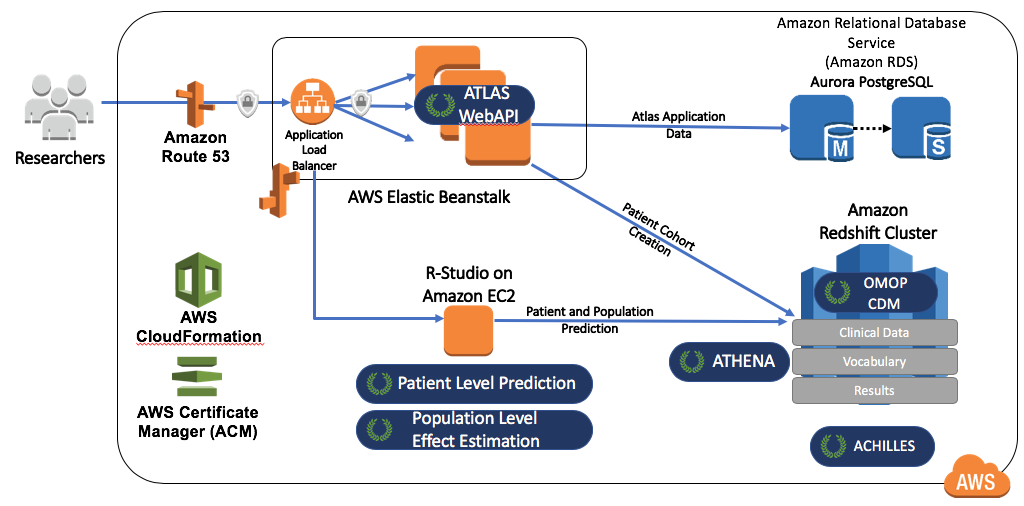
\includegraphics[width=1\linewidth]{images/OhdsiAnalyticsTools/OHDSIonAWSDiagram} 

}

\caption{The Amazon Web Services architecture for OHDSIonAWS.}\label{fig:ohdsionawsDiagram}
\end{figure}

\section{Résumé}\label{ruxe9sumuxe9-6}

\begin{rmdsummary}
\begin{itemize}
\tightlist
\item
  Nous pouvons effectuer des analyses sur les données du CDM en

  \begin{itemize}
  \tightlist
  \item
    écrivant du code personnalisé
  \item
    écrivant du code qui utilise les packages R dans la Méthode Bibliothèque OHDSI
  \item
    utilisant la plateforme d'analyse interactive ATLAS
  \end{itemize}
\item
  Les outils OHDSI utilisent différentes stratégies d'analyse

  \begin{itemize}
  \tightlist
  \item
    Études uniques
  \item
    Requêtes en temps réel
  \item
    Analytique à grande échelle
  \end{itemize}
\item
  La majorité des outils analytiques OHDSI sont intégrés dans

  \begin{itemize}
  \tightlist
  \item
    La plateforme d'analyse interactive ATLAS
  \item
    Les packages R de la Méthode Bibliothèque OHDSI
  \end{itemize}
\item
  Plusieurs stratégies existent pour faciliter le déploiement des outils OHDSI.
\end{itemize}
\end{rmdsummary}

\chapter{SQL et R}\label{SqlAndR}

\emph{Responsables de chapitre : Martijn Schuemie \& Peter Rijnbeek}

Le Common Data Model (CDM) est un modèle de base de données relationnelle (toutes les données sont représentées sous forme d'enregistrements dans des tables qui ont des champs), ce qui signifie que les données seront normalement stockées dans une base de données relationnelle utilisant une plateforme logicielle comme PostgreSQL, Oracle ou Microsoft SQL Server. Les divers outils OHDSI tels que ATLAS et la Methods Library fonctionnent en interrogeant la base de données en coulisse, mais nous pouvons également interroger directement la base de données nous-mêmes si nous disposons des droits d'accès appropriés. La principale raison de le faire est d'effectuer des analyses qui ne sont actuellement pas supportées par des outils existants. Cependant, interroger directement la base de données comporte également un risque accru de faire des erreurs, car les outils OHDSI sont souvent conçus pour aider à guider l'utilisateur vers une analyse appropriée des données. Les requêtes directes ne fournissent pas une telle guidance.

Le langage standard pour interroger les bases de données relationnelles est le SQL (Structured Query Language), qui peut être utilisé à la fois pour interroger la base de données ainsi que pour apporter des modifications aux données. Bien que les commandes de base en SQL soient en effet standard, c'est-à-dire les mêmes sur toutes les plateformes logicielles, chaque plateforme a son propre dialecte, avec des différences subtiles. Par exemple, pour récupérer les 10 premières lignes de la table PERSON sur SQL Server, on écrirait : \index{SQL} \index{structured query language|see {SQL}}

\begin{Shaded}
\begin{Highlighting}[]
\KeywordTok{SELECT}\NormalTok{ TOP }\DecValTok{10} \OperatorTok{*} \KeywordTok{FROM}\NormalTok{ person;}
\end{Highlighting}
\end{Shaded}

Tandis que la même requête sur PostgreSQL serait :

\begin{Shaded}
\begin{Highlighting}[]
\KeywordTok{SELECT} \OperatorTok{*} \KeywordTok{FROM}\NormalTok{ person }\KeywordTok{LIMIT} \DecValTok{10}\NormalTok{;}
\end{Highlighting}
\end{Shaded}

Dans OHDSI, nous aimerions être agnostiques vis-à-vis du dialecte spécifique qu'une plateforme utilise ; nous aimerions `parler' le même langage SQL sur toutes les bases de données OHDSI. Pour cette raison, OHDSI a développé le package \href{https://ohdsi.github.io/SqlRender/}{SqlRender}, un package R qui peut traduire d'un dialecte standard vers n'importe lequel des dialectes supportés qui seront discutés plus tard dans ce chapitre. Ce dialecte standard - \textbf{OHDSI SQL} - est principalement un sous-ensemble du dialecte SQL Server SQL. Les exemples de déclarations SQL fournis tout au long de ce chapitre utiliseront tous l'OHDSI SQL. \index{SqlRender} \index{agnostic SQL|see {SqlRender}} \index{Standard SQL Dialect|see {SqlRender}} \index{OHDSI SQL|see {SqlRender}}

Chaque plateforme de base de données dispose également de ses propres outils logiciels pour interroger la base de données en utilisant SQL. Dans OHDSI, nous avons développé le package \href{https://ohdsi.github.io/DatabaseConnector/}{DatabaseConnector}, un package R qui peut se connecter à de nombreuses plateformes de base de données. DatabaseConnector sera également discuté plus tard dans ce chapitre. \index{DatabaseConnector}

Ainsi, bien que l'on puisse interroger une base de données conforme au CDM sans utiliser d'outils OHDSI, le chemin recommandé est d'utiliser les packages DatabaseConnector et SqlRender. Cela permet aux requêtes développées sur un site d'être utilisées sur n'importe quel autre site sans modification. R lui-même offre également immédiatement des fonctionnalités pour analyser davantage les données extraites de la base de données, telles que la réalisation d'analyses statistiques et la génération de graphiques (interactifs). \index{R}

Dans ce chapitre, nous supposons que le lecteur a une compréhension de base de SQL. Nous passons d'abord en revue comment utiliser SqlRender et DatabaseConnector. Si le lecteur n'a pas l'intention d'utiliser ces packages, ces sections peuvent être omises. Dans la Section \ref{QueryTheCdm}, nous discutons de la manière d'utiliser SQL (dans ce cas OHDSI SQL) pour interroger le CDM. La section suivante met en lumière comment utiliser le Vocabulaire Standardisé OHDSI lors de l'interrogation du CDM. Nous mettons en avant la QueryLibrary, une collection de requêtes couramment utilisées contre le CDM qui est publiquement disponible. Nous clôturons ce chapitre avec une étude exemple estimant les taux d'incidence, et implémentons cette étude en utilisant SqlRender et DatabaseConnector. \index{Query Library} \index{SQL Query Library|see {Query Library}}

\section{SqlRender}\label{SqlRender}

Le package \href{https://ohdsi.github.io/SqlRender/}{SqlRender} est disponible sur CRAN (le Comprehensive R Archive Network), et peut donc être installé en utilisant :

\begin{Shaded}
\begin{Highlighting}[]
\FunctionTok{install.packages}\NormalTok{(}\StringTok{"SqlRender"}\NormalTok{)}
\end{Highlighting}
\end{Shaded}

SqlRender prend en charge une large gamme de plateformes techniques, y compris les systèmes de bases de données traditionnels (PostgreSQL, Microsoft SQL Server, SQLite et Oracle), les entrepôts de données parallèles (Microsoft APS, IBM Netezza et Amazon Redshift), ainsi que les plateformes Big Data (Hadoop via Impala et Google BigQuery). Le package R est fourni avec un manuel et une vignette qui explore toutes les fonctionnalités. Ici, nous décrivons certaines des principales fonctionnalités.

\subsection{Paramétrage SQL}\label{paramuxe9trage-sql}

Une des fonctions du package est de prendre en charge la paramétrisation du SQL. Souvent, de petites variations du SQL doivent être générées en fonction de certains paramètres. SqlRender offre une syntaxe de balisage simple dans le code SQL pour permettre la paramétrisation. Le rendu du SQL basé sur les valeurs des paramètres est effectué à l'aide de la fonction \texttt{render()}. \index{SqlRender!parameterization}

\subsubsection*{Substitution des Valeurs de Paramètres}\label{substitution-des-valeurs-de-paramuxe8tres}
\addcontentsline{toc}{subsubsection}{Substitution des Valeurs de Paramètres}

Le caractère \texttt{@} peut être utilisé pour indiquer les noms des paramètres à échanger contre les valeurs réelles des paramètres lors du rendu. Dans l'exemple suivant, une variable appelée \texttt{a} est mentionnée dans le SQL. Dans l'appel à la fonction render, la valeur de ce paramètre est définie :

\begin{Shaded}
\begin{Highlighting}[]
\NormalTok{sql }\OtherTok{\textless{}{-}} \StringTok{"SELECT * FROM concept WHERE concept\_id = @a;"}
\FunctionTok{render}\NormalTok{(sql, }\AttributeTok{a =} \DecValTok{123}\NormalTok{)}
\end{Highlighting}
\end{Shaded}

\begin{verbatim}
## [1] "SELECT * FROM concept WHERE concept_id = 123;"
\end{verbatim}

Notez que, contrairement à la paramétrisation offerte par la plupart des systèmes de gestion de bases de données, il est tout aussi facile de paramétrer les noms de tables ou de champs que les valeurs :

\begin{Shaded}
\begin{Highlighting}[]
\NormalTok{sql }\OtherTok{\textless{}{-}} \StringTok{"SELECT * FROM @x WHERE person\_id = @a;"}
\FunctionTok{render}\NormalTok{(sql, }\AttributeTok{x =} \StringTok{"observation"}\NormalTok{, }\AttributeTok{a =} \DecValTok{123}\NormalTok{)}
\end{Highlighting}
\end{Shaded}

\begin{verbatim}
## [1] "SELECT * FROM observation WHERE person_id = 123;"
\end{verbatim}

Les valeurs des paramètres peuvent être des nombres, des chaînes, des booléens ainsi que des vecteurs, qui sont convertis en listes séparées par des virgules :

\begin{Shaded}
\begin{Highlighting}[]
\NormalTok{sql }\OtherTok{\textless{}{-}} \StringTok{"SELECT * FROM concept WHERE concept\_id IN (@a);"}
\FunctionTok{render}\NormalTok{(sql, }\AttributeTok{a =} \FunctionTok{c}\NormalTok{(}\DecValTok{123}\NormalTok{, }\DecValTok{234}\NormalTok{, }\DecValTok{345}\NormalTok{))}
\end{Highlighting}
\end{Shaded}

\begin{verbatim}
## [1] "SELECT * FROM concept WHERE concept_id IN (123,234,345);"
\end{verbatim}

\subsubsection*{If-Then-Else}\label{if-then-else}
\addcontentsline{toc}{subsubsection}{If-Then-Else}

Parfois, des blocs de codes doivent être activés ou désactivés en fonction des valeurs d'un ou plusieurs paramètres. Cela se fait en utilisant la syntaxe \texttt{\{Condition\}\ ?\ \{if\ true\}\ :\ \{if\ false\}}. Si la \emph{condition} évalue à true ou 1, le bloc \emph{if true} est utilisé, sinon le bloc \emph{if false} est affiché (s'il est présent).

\begin{Shaded}
\begin{Highlighting}[]
\NormalTok{sql }\OtherTok{\textless{}{-}} \StringTok{"SELECT * FROM cohort \{@x\} ? \{WHERE subject\_id = 1\}"}
\FunctionTok{render}\NormalTok{(sql, }\AttributeTok{x =} \ConstantTok{FALSE}\NormalTok{)}
\end{Highlighting}
\end{Shaded}

\begin{verbatim}
## [1] "SELECT * FROM cohort "
\end{verbatim}

\begin{Shaded}
\begin{Highlighting}[]
\FunctionTok{render}\NormalTok{(sql, }\AttributeTok{x =} \ConstantTok{TRUE}\NormalTok{)}
\end{Highlighting}
\end{Shaded}

\begin{verbatim}
## [1] "SELECT * FROM cohort WHERE subject_id = 1"
\end{verbatim}

Les comparaisons simples sont également prises en charge :

\begin{Shaded}
\begin{Highlighting}[]
\NormalTok{sql }\OtherTok{\textless{}{-}} \StringTok{"SELECT * FROM cohort \{@x == 1\} ? \{WHERE subject\_id = 1\};"}
\FunctionTok{render}\NormalTok{(sql, }\AttributeTok{x =} \DecValTok{1}\NormalTok{)}
\end{Highlighting}
\end{Shaded}

\begin{verbatim}
## [1] "SELECT * FROM cohort WHERE subject_id = 1;"
\end{verbatim}

\begin{Shaded}
\begin{Highlighting}[]
\FunctionTok{render}\NormalTok{(sql, }\AttributeTok{x =} \DecValTok{2}\NormalTok{)}
\end{Highlighting}
\end{Shaded}

\begin{verbatim}
## [1] "SELECT * FROM cohort ;"
\end{verbatim}

Ainsi que l'opérateur \texttt{IN} :

\begin{Shaded}
\begin{Highlighting}[]
\NormalTok{sql }\OtherTok{\textless{}{-}} \StringTok{"SELECT * FROM cohort \{@x IN (1,2,3)\} ? \{WHERE subject\_id = 1\};"}
\FunctionTok{render}\NormalTok{(sql, }\AttributeTok{x =} \DecValTok{2}\NormalTok{)}
\end{Highlighting}
\end{Shaded}

\begin{verbatim}
## [1] "SELECT * FROM cohort WHERE subject_id = 1;"
\end{verbatim}

\subsection{Traduction vers d'Autres Dialectes SQL}\label{traduction-vers-dautres-dialectes-sql}

Une autre fonction du package \href{https://ohdsi.github.io/SqlRender/}{SqlRender} est de traduire du SQL OHDSI vers d'autres dialectes SQL. Par exemple :

\begin{Shaded}
\begin{Highlighting}[]
\NormalTok{sql }\OtherTok{\textless{}{-}} \StringTok{"SELECT TOP 10 * FROM person;"}
\FunctionTok{translate}\NormalTok{(sql, }\AttributeTok{targetDialect =} \StringTok{"postgresql"}\NormalTok{)}
\end{Highlighting}
\end{Shaded}

\begin{verbatim}
## [1] "SELECT  * FROM person LIMIT 10;"
## attr(,"sqlDialect")
## [1] "postgresql"
\end{verbatim}

Le paramètre \texttt{targetDialect} peut avoir les valeurs suivantes : ``oracle'', ``postgresql'', ``pdw'', ``redshift'', ``impala'', ``netezza'', ``bigquery'', ``sqlite'' et ``sql server''. \index{SqlRender!translation}

\begin{rmdimportant}
Il existe des limites quant à ce que les fonctions et constructions SQL peuvent être traduites correctement, à la fois parce qu'un ensemble limité de règles de traduction ont été implémentées dans le package, mais aussi parce que certaines fonctionnalités SQL n'ont pas d'équivalent dans tous les dialectes. Ceci est la raison principale pour laquelle le SQL OHDSI a été développé en tant que nouveau dialecte SQL à part entière. Cependant, chaque fois que possible, nous avons gardé la syntaxe SQL Server pour éviter de réinventer la roue.
\end{rmdimportant}

Malgré nos meilleurs efforts, il y a beaucoup de considérations à prendre en compte lors de l'écriture de SQL OHDSI qui s'exécutera sans erreur sur toutes les plateformes prises en charge. Ce qui suit discute de ces considérations en détail.

\subsubsection*{Fonctions et Structures Prises en Charge par Translate}\label{fonctions-et-structures-prises-en-charge-par-translate}
\addcontentsline{toc}{subsubsection}{Fonctions et Structures Prises en Charge par Translate}

Ces fonctions SQL Server ont été testées et se sont révélées être correctement traduites dans les différents dialectes : \index{SqlRender!supported functions}

Table : \label{tab:sqlFunctions} Fonctions prises en charge par translate.

\begin{longtable}[]{@{}lll@{}}
\toprule\noalign{}
Fonction & Fonction & Fonction \\
\midrule\noalign{}
\endhead
\bottomrule\noalign{}
\endlastfoot
ABS & EXP & RAND \\
ACOS & FLOOR & RANK \\
ASIN & GETDATE & RIGHT \\
ATAN & HASHBYTES* & ROUND \\
AVG & ISNULL & ROW\_NUMBER \\
CAST & ISNUMERIC & RTRIM \\
CEILING & LEFT & SIN \\
CHARINDEX & LEN & SQRT \\
CONCAT & LOG & SQUARE \\
COS & LOG10 & STDEV \\
COUNT & LOWER & SUM \\
COUNT\_BIG & LTRIM & TAN \\
DATEADD & MAX & UPPER \\
DATEDIFF & MIN & VAR \\
DATEFROMPARTS & MONTH & YEAR \\
DATETIMEFROMPARTS & NEWID & \\
DAY & PI & \\
EOMONTH & POWER & \\
\end{longtable}

* Nécessite des privilèges spéciaux sur Oracle. N'a pas d'équivalent sur SQLite.

De même, de nombreuses structures syntaxiques SQL sont prises en charge. Voici une liste non exhaustive d'expressions dont nous savons qu'elles se traduisent bien :

\begin{Shaded}
\begin{Highlighting}[]
\CommentTok{{-}{-} Sélections simples :}
\KeywordTok{SELECT} \OperatorTok{*} \KeywordTok{FROM} \KeywordTok{table}\NormalTok{;}

\CommentTok{{-}{-} Sélections avec jointures :}
\KeywordTok{SELECT} \OperatorTok{*} \KeywordTok{FROM}\NormalTok{ table\_1 }\KeywordTok{INNER} \KeywordTok{JOIN}\NormalTok{ table\_2 }\KeywordTok{ON}\NormalTok{ a }\OperatorTok{=}\NormalTok{ b;}

\CommentTok{{-}{-} Requêtes imbriquées :}
\KeywordTok{SELECT} \OperatorTok{*} \KeywordTok{FROM}\NormalTok{ (}\KeywordTok{SELECT} \OperatorTok{*} \KeywordTok{FROM}\NormalTok{ table\_1) tmp }\KeywordTok{WHERE}\NormalTok{ a }\OperatorTok{=}\NormalTok{ b;}

\CommentTok{{-}{-} Limitation aux lignes du haut :}
\KeywordTok{SELECT}\NormalTok{ TOP }\DecValTok{10} \OperatorTok{*} \KeywordTok{FROM} \KeywordTok{table}\NormalTok{;}

\CommentTok{{-}{-} Sélection dans une nouvelle table :}
\KeywordTok{SELECT} \OperatorTok{*} \KeywordTok{INTO}\NormalTok{ new\_table }\KeywordTok{FROM} \KeywordTok{table}\NormalTok{;}

\CommentTok{{-}{-} Création de tables :}
\KeywordTok{CREATE} \KeywordTok{TABLE} \KeywordTok{table}\NormalTok{ (field }\DataTypeTok{INT}\NormalTok{);}

\CommentTok{{-}{-} Insertion de valeurs littérales :}
\KeywordTok{INSERT} \KeywordTok{INTO}\NormalTok{ other\_table (field\_1) }\KeywordTok{VALUES}\NormalTok{ (}\DecValTok{1}\NormalTok{);}

\CommentTok{{-}{-} Insertion à partir de SELECT :}
\KeywordTok{INSERT} \KeywordTok{INTO}\NormalTok{ other\_table (field\_1) }\KeywordTok{SELECT} \FunctionTok{value} \KeywordTok{FROM} \KeywordTok{table}\NormalTok{;}

\CommentTok{{-}{-} Commandes de suppression simples :}
\KeywordTok{DROP} \KeywordTok{TABLE} \KeywordTok{table}\NormalTok{;}

\CommentTok{{-}{-} Suppression de table si elle existe :}
\ControlFlowTok{IF}\NormalTok{ OBJECT\_ID(}\StringTok{\textquotesingle{}ACHILLES\_analysis\textquotesingle{}}\NormalTok{, }\StringTok{\textquotesingle{}U\textquotesingle{}}\NormalTok{) }\KeywordTok{IS} \KeywordTok{NOT} \KeywordTok{NULL}
  \KeywordTok{DROP} \KeywordTok{TABLE}\NormalTok{ ACHILLES\_analysis;}

\CommentTok{{-}{-} Suppression de table temporaire si elle existe :}
\ControlFlowTok{IF}\NormalTok{ OBJECT\_ID(}\StringTok{\textquotesingle{}tempdb..\#cohorts\textquotesingle{}}\NormalTok{, }\StringTok{\textquotesingle{}U\textquotesingle{}}\NormalTok{) }\KeywordTok{IS} \KeywordTok{NOT} \KeywordTok{NULL}
  \KeywordTok{DROP} \KeywordTok{TABLE}\NormalTok{ \#cohorts;}

\CommentTok{{-}{-} Expressions de table communes :}
\KeywordTok{WITH}\NormalTok{ cte }\KeywordTok{AS}\NormalTok{ (}\KeywordTok{SELECT} \OperatorTok{*} \KeywordTok{FROM} \KeywordTok{table}\NormalTok{) }\KeywordTok{SELECT} \OperatorTok{*} \KeywordTok{FROM}\NormalTok{ cte;}

\CommentTok{{-}{-} Clauses OVER :}
\KeywordTok{SELECT} \FunctionTok{ROW\_NUMBER}\NormalTok{() }\KeywordTok{OVER}\NormalTok{ (}\KeywordTok{PARTITION} \KeywordTok{BY}\NormalTok{ a }\KeywordTok{ORDER} \KeywordTok{BY}\NormalTok{ b)}
  \KeywordTok{AS} \OtherTok{"Row Number"} \KeywordTok{FROM} \KeywordTok{table}\NormalTok{;}

\CommentTok{{-}{-} Clauses CASE WHEN :}
\KeywordTok{SELECT} \ControlFlowTok{CASE} \ControlFlowTok{WHEN}\NormalTok{ a}\OperatorTok{=}\DecValTok{1} \ControlFlowTok{THEN}\NormalTok{ a }\ControlFlowTok{ELSE} \DecValTok{0} \ControlFlowTok{END} \KeywordTok{AS} \FunctionTok{value} \KeywordTok{FROM} \KeywordTok{table}\NormalTok{;}

\CommentTok{{-}{-} UNIONS :}
\KeywordTok{SELECT} \OperatorTok{*} \KeywordTok{FROM}\NormalTok{ a }\KeywordTok{UNION} \KeywordTok{SELECT} \OperatorTok{*} \KeywordTok{FROM}\NormalTok{ b;}

\CommentTok{{-}{-} INTERSECTIONS :}
\KeywordTok{SELECT} \OperatorTok{*} \KeywordTok{FROM}\NormalTok{ a }\KeywordTok{INTERSECT} \KeywordTok{SELECT} \OperatorTok{*} \KeywordTok{FROM}\NormalTok{ b;}

\CommentTok{{-}{-} EXCEPT :}
\KeywordTok{SELECT} \OperatorTok{*} \KeywordTok{FROM}\NormalTok{ a }\KeywordTok{EXCEPT} \KeywordTok{SELECT} \OperatorTok{*} \KeywordTok{FROM}\NormalTok{ b;}
\end{Highlighting}
\end{Shaded}

\subsubsection*{Concaténation de Chaînes}\label{concatuxe9nation-de-chauxeenes}
\addcontentsline{toc}{subsubsection}{Concaténation de Chaînes}

La concaténation de chaînes est un domaine où SQL Server est moins spécifique que d'autres dialectes. Dans SQL Server, on écrirait \texttt{SELECT\ first\_name\ +\ \textquotesingle{}\ \textquotesingle{}\ +\ last\_name\ AS\ full\_name\ FROM\ table}, mais cela devrait être \texttt{SELECT\ first\_name\ \textbar{}\textbar{}\ \textquotesingle{}\ \textquotesingle{}\ \textbar{}\textbar{}\ last\_name\ AS\ full\_name\ FROM\ table} dans PostgreSQL et Oracle. SqlRender tente de deviner quand les valeurs concaténées sont des chaînes. Dans l'exemple ci-dessus, parce que nous avons une chaîne explicite (l'espace entouré de guillemets simples), la traduction sera correcte. Cependant, si la requête avait été \texttt{SELECT\ first\_name\ +\ last\_name\ AS\ full\_name\ FROM\ table}, SqlRender n'aurait pas eu d'indice que les deux champs étaient des chaînes, et laisserait incorrectement le signe plus. Un autre indice qu'une valeur est une chaîne est une conversion explicite en VARCHAR, donc \texttt{SELECT\ last\_name\ +\ CAST(age\ AS\ VARCHAR(3))\ AS\ full\_name\ FROM\ table} serait également traduit correctement. Pour éviter toute ambiguïté, il est probablement préférable d'utiliser la fonction \texttt{CONCAT()} pour concaténer deux ou plusieurs chaînes.

\subsubsection*{Alias de Table et le Mot-Clé AS}\label{alias-de-table-et-le-mot-cluxe9-as}
\addcontentsline{toc}{subsubsection}{Alias de Table et le Mot-Clé AS}

De nombreux dialectes SQL permettent l'utilisation du mot-clé \texttt{AS} lors de la définition d'un alias de table, mais fonctionneront également bien sans le mot-clé. Par exemple, ces deux instructions SQL sont correctes pour SQL Server, PostgreSQL, Redshift, etc. :

\begin{Shaded}
\begin{Highlighting}[]
\CommentTok{{-}{-} Utilisation du mot{-}clé AS}
\KeywordTok{SELECT} \OperatorTok{*}
\KeywordTok{FROM}\NormalTok{ my\_table }\KeywordTok{AS}\NormalTok{ table\_1}
\KeywordTok{INNER} \KeywordTok{JOIN}\NormalTok{ (}
  \KeywordTok{SELECT} \OperatorTok{*} \KeywordTok{FROM}\NormalTok{ other\_table}
\NormalTok{) }\KeywordTok{AS}\NormalTok{ table\_2}
\KeywordTok{ON}\NormalTok{ table\_1.person\_id }\OperatorTok{=}\NormalTok{ table\_2.person\_id;}

\CommentTok{{-}{-} Non{-}utilisation du mot{-}clé AS}
\KeywordTok{SELECT} \OperatorTok{*}
\KeywordTok{FROM}\NormalTok{ my\_table table\_1}
\KeywordTok{INNER} \KeywordTok{JOIN}\NormalTok{ (}
  \KeywordTok{SELECT} \OperatorTok{*} \KeywordTok{FROM}\NormalTok{ other\_table}
\NormalTok{) table\_2}
\KeywordTok{ON}\NormalTok{ table\_1.person\_id }\OperatorTok{=}\NormalTok{ table\_2.person\_id;}
\end{Highlighting}
\end{Shaded}

Cependant, Oracle renverra une erreur lorsque le mot-clé \texttt{AS} est utilisé. Dans l'exemple ci-dessus, la première requête échouera. Il est donc recommandé de ne pas utiliser le mot-clé \texttt{AS} lors de la création d'alias de tables. (Note : nous ne pouvons pas faire en sorte que SqlRender gère cela, car il ne peut pas facilement distinguer entre les alias de tables où Oracle n'autorise pas l'utilisation de \texttt{AS}, et les alias de champs, où Oracle nécessite l'utilisation de \texttt{AS}.)

\subsubsection*{Tables Temporaires}\label{tables-temporaires}
\addcontentsline{toc}{subsubsection}{Tables Temporaires}

Les tables temporaires peuvent être très utiles pour stocker des résultats intermédiaires, et lorsqu'elles sont utilisées correctement, elles peuvent améliorer considérablement les performances des requêtes. Sur la plupart des plateformes de bases de données, les tables temporaires présentent de très belles propriétés : elles ne sont visibles que par l'utilisateur actuel, sont automatiquement supprimées lorsque la session se termine et peuvent être créées même lorsque l'utilisateur n'a pas d'accès en écriture. Malheureusement, dans Oracle, les tables temporaires sont essentiellement des tables permanentes, avec la seule différence que les données à l'intérieur de la table ne sont visibles que par l'utilisateur actuel. C'est pourquoi, dans Oracle, SqlRender essaiera d'émuler les tables temporaires en

\begin{enumerate}
\def\labelenumi{\arabic{enumi}.}
\tightlist
\item
  Ajoutant une chaîne aléatoire au nom de la table afin que les tables de différents utilisateurs ne soient pas en conflit.
\item
  Permettant à l'utilisateur de spécifier le schéma où les tables temporaires seront créées.
\end{enumerate}

Par exemple :

\begin{Shaded}
\begin{Highlighting}[]
\NormalTok{sql }\OtherTok{\textless{}{-}} \StringTok{"SELECT * FROM \#children;"}
\FunctionTok{translate}\NormalTok{(sql, }\AttributeTok{targetDialect =} \StringTok{"oracle"}\NormalTok{, }\AttributeTok{oracleTempSchema =} \StringTok{"temp\_schema"}\NormalTok{)}
\end{Highlighting}
\end{Shaded}

\begin{verbatim}
## Warning: The 'oracleTempSchema' argument is deprecated. Use 'tempEmulationSchema' instead.
## This warning is displayed once every 8 hours.
\end{verbatim}

\begin{verbatim}
## [1] "SELECT * FROM temp_schema.tt0id3pachildren ;"
## attr(,"sqlDialect")
## [1] "oracle"
\end{verbatim}

Notez que l'utilisateur devra avoir des privilèges d'écriture sur \texttt{temp\_schema}.

Notez également que, parce qu'Oracle a une limite de 30 caractères pour les noms de table, \textbf{les noms de tables temporaires ne sont autorisés à avoir que 22 caractères maximum}, car sinon le nom deviendra trop long après l'ajout de l'ID de session.

De plus, rappelez-vous que les tables temporaires ne sont pas automatiquement supprimées sur Oracle, vous devrez donc explicitement \texttt{TRUNCATE} et \texttt{DROP} toutes les tables temporaires une fois que vous avez terminé avec elles pour éviter que des tables orphelines ne s'accumulent dans le schéma temporaire Oracle.

\subsubsection*{Conversions Implicites}\label{conversions-implicites}
\addcontentsline{toc}{subsubsection}{Conversions Implicites}

L'un des rares points où SQL Server est moins explicite que d'autres dialectes est qu'il permet les conversions implicites. Par exemple, ce code fonctionnera sur SQL Server :

\begin{Shaded}
\begin{Highlighting}[]
\KeywordTok{CREATE} \KeywordTok{TABLE}\NormalTok{ \#temp (txt }\DataTypeTok{VARCHAR}\NormalTok{);}

\KeywordTok{INSERT} \KeywordTok{INTO}\NormalTok{ \#temp}
\KeywordTok{SELECT} \StringTok{\textquotesingle{}1\textquotesingle{}}\NormalTok{;}

\KeywordTok{SELECT} \OperatorTok{*} \KeywordTok{FROM}\NormalTok{ \#temp }\KeywordTok{WHERE}\NormalTok{ txt }\OperatorTok{=} \DecValTok{1}\NormalTok{;}
\end{Highlighting}
\end{Shaded}

Même si \texttt{txt} est un champ VARCHAR et que nous le comparons à un entier, SQL Server convertira automatiquement l'une des deux au type correct pour permettre la comparaison. En revanche, d'autres dialectes comme PostgreSQL renverront une erreur lorsqu'ils essaieront de comparer un VARCHAR avec un INT.

Vous devez donc toujours rendre les conversions explicites. Dans l'exemple ci-dessus, la dernière instruction doit être remplacée par soit

\begin{Shaded}
\begin{Highlighting}[]
\KeywordTok{SELECT} \OperatorTok{*} \KeywordTok{FROM}\NormalTok{ \#temp }\KeywordTok{WHERE}\NormalTok{ txt }\OperatorTok{=} \FunctionTok{CAST}\NormalTok{(}\DecValTok{1} \KeywordTok{AS} \DataTypeTok{VARCHAR}\NormalTok{);}
\end{Highlighting}
\end{Shaded}

ou

\begin{Shaded}
\begin{Highlighting}[]
\KeywordTok{SELECT} \OperatorTok{*} \KeywordTok{FROM}\NormalTok{ \#temp }\KeywordTok{WHERE} \FunctionTok{CAST}\NormalTok{(txt }\KeywordTok{AS} \DataTypeTok{INT}\NormalTok{) }\OperatorTok{=} \DecValTok{1}\NormalTok{;}
\end{Highlighting}
\end{Shaded}

\subsubsection*{Sensibilité à la Casse dans les Comparaisons de Chaînes}\label{sensibilituxe9-uxe0-la-casse-dans-les-comparaisons-de-chauxeenes}
\addcontentsline{toc}{subsubsection}{Sensibilité à la Casse dans les Comparaisons de Chaînes}

Certaines plateformes SGBD comme SQL Server effectuent toujours des comparaisons de chaînes de manière insensible à la casse, tandis que d'autres comme PostgreSQL sont toujours sensibles à la casse. Il est donc recommandé de toujours supposer des comparaisons sensibles à la casse, et de rendre explicitement les comparaisons insensibles à la casse lorsqu'on n'est pas sûr de la casse. Par exemple, au lieu de

\begin{Shaded}
\begin{Highlighting}[]
\KeywordTok{SELECT} \OperatorTok{*} \KeywordTok{FROM}\NormalTok{ concept }\KeywordTok{WHERE}\NormalTok{ concept\_class\_id }\OperatorTok{=} \StringTok{\textquotesingle{}Clinical Finding\textquotesingle{}}
\end{Highlighting}
\end{Shaded}

il est préférable d'utiliser

\begin{Shaded}
\begin{Highlighting}[]
\KeywordTok{SELECT} \OperatorTok{*} \KeywordTok{FROM}\NormalTok{ concept }\KeywordTok{WHERE} \FunctionTok{LOWER}\NormalTok{(concept\_class\_id) }\OperatorTok{=} \StringTok{\textquotesingle{}clinical finding\textquotesingle{}}
\end{Highlighting}
\end{Shaded}

\subsubsection*{Schémas et Bases de Données}\label{schuxe9mas-et-bases-de-donnuxe9es}
\addcontentsline{toc}{subsubsection}{Schémas et Bases de Données}

Dans SQL Server, les tables sont situées dans un schéma, et les schémas résident dans une base de données. Par exemple, \texttt{cdm\_data.dbo.person} fait référence à la table \texttt{person} dans le schéma \texttt{dbo} dans la base de données \texttt{cdm\_data}. Dans d'autres dialectes, bien qu'une hiérarchie similaire existe souvent, elle est utilisée de manière très différente. Dans SQL Server, il y a généralement un schéma par base de données (souvent appelé \texttt{dbo}), et les utilisateurs peuvent facilement utiliser des données dans différentes bases de données. Sur d'autres plateformes, par exemple dans PostgreSQL, il n'est pas possible d'utiliser des données entre différentes bases de données dans une seule session, mais il y a souvent de nombreux schémas dans une base de données. Dans PostgreSQL, on pourrait dire que l'équivalent de la base de données de SQL Server est le schéma.

Nous recommandons donc de concaténer la base de données et le schéma de SQL Server en un seul paramètre, que nous appelons généralement \texttt{@databaseSchema}. Par exemple, nous pourrions avoir le SQL paramétré

\begin{Shaded}
\begin{Highlighting}[]
\KeywordTok{SELECT} \OperatorTok{*} \KeywordTok{FROM}\NormalTok{ @databaseSchema.person}
\end{Highlighting}
\end{Shaded}

où sur SQL Server nous pouvons inclure à la fois les noms de base de données et de schéma dans la valeur : \texttt{databaseSchema\ =\ "cdm\_data.dbo"}. Sur d'autres plateformes, nous pouvons utiliser le même code, mais maintenant seulement spécifier le schéma comme valeur du paramètre : \texttt{databaseSchema\ =\ "cdm\_data"}.

La seule situation où cela échouera est la commande \texttt{USE}, puisque \texttt{USE\ cdm\_data.dbo;} renverra une erreur. Il est donc préférable de ne pas utiliser la commande \texttt{USE}, mais de toujours spécifier la base de données / le schéma où une table est située.

\subsubsection*{Débogage de SQL Paramétré}\label{duxe9bogage-de-sql-paramuxe9truxe9}
\addcontentsline{toc}{subsubsection}{Débogage de SQL Paramétré}

Le débogage de SQL paramétré peut être un peu compliqué. Seul le SQL rendu peut être testé contre un serveur de base de données, mais les modifications du code doivent être effectuées dans le SQL paramétré (pré-rendu). \index{SqlRender!debugging}

Une application Shiny est incluse dans le package SqlRender pour éditer de façon interactive le SQL source et générer du SQL rendu et traduit. L'application peut être lancée en utilisant :

\begin{Shaded}
\begin{Highlighting}[]
\FunctionTok{launchSqlRenderDeveloper}\NormalTok{()}
\end{Highlighting}
\end{Shaded}

Cela ouvrira le navigateur par défaut avec l'application montrée sur la Figure \ref{fig:sqlDeveloper}. L'application est également disponible publiquement sur le web.\footnote{\url{http://data.ohdsi.org/SqlDeveloper/}}

\begin{figure}

{\centering 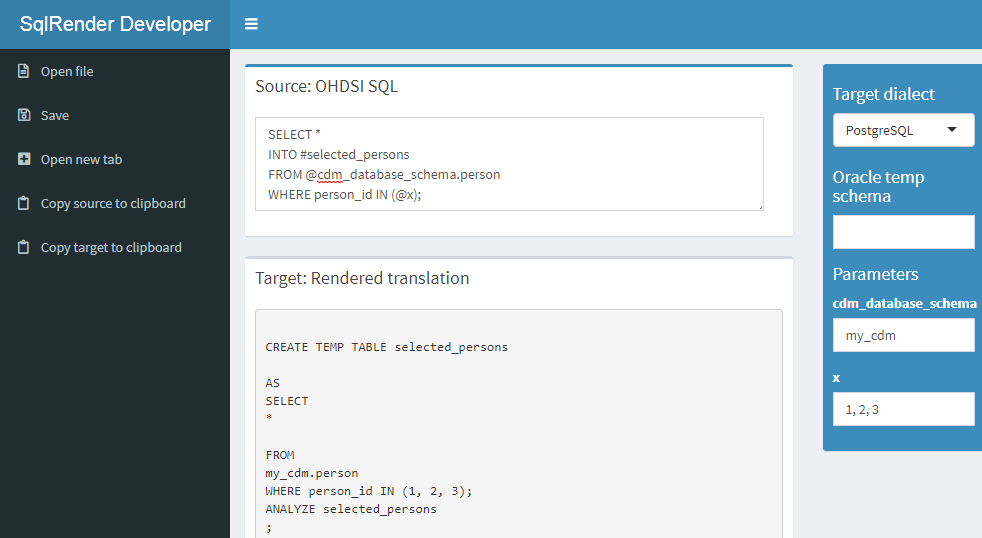
\includegraphics[width=1\linewidth]{images/SqlAndR/sqlDeveloper} 

}

\caption{The SqlDeveloper Shiny app.}\label{fig:sqlDeveloper}
\end{figure}

Dans l'application, vous pouvez entrer du SQL OHDSI, sélectionner le dialecte cible ainsi que fournir des valeurs pour les paramètres qui apparaissent dans votre SQL, et la traduction apparaîtra automatiquement en bas.

\section{DatabaseConnector}\label{DatabaseConnector}

\href{https://ohdsi.github.io/DatabaseConnector/}{DatabaseConnector} est un package R pour se connecter à diverses plateformes de bases de données en utilisant les pilotes JDBC de Java. Le package DatabaseConnector est disponible sur CRAN (le Comprehensive R Archive Network), et peut donc être installé en utilisant :

\begin{Shaded}
\begin{Highlighting}[]
\FunctionTok{install.packages}\NormalTok{(}\StringTok{"DatabaseConnector"}\NormalTok{)}
\end{Highlighting}
\end{Shaded}

DatabaseConnector prend en charge un large éventail de plateformes techniques, y compris les systèmes de bases de données traditionnels (PostgreSQL, Microsoft SQL Server, SQLite, et Oracle), les entrepôts de données parallèles (Microsoft APS, IBM Netezza, et Amazon), ainsi que les plateformes Big Data (Hadoop via Impala, et Google BigQuery). Le package contient déjà la plupart des pilotes, mais en raison de raisons de licence, les pilotes pour BigQuery, Netezza et Impala ne sont pas inclus et doivent être obtenus par l'utilisateur. Tapez \texttt{?jdbcDrivers} pour des instructions sur la manière de télécharger ces pilotes. Une fois téléchargés, vous pouvez utiliser l'argument \texttt{pathToDriver} des fonctions \texttt{connect}, \texttt{dbConnect}, et \texttt{createConnectionDetails}.

\subsection{Création d'une Connexion}\label{cruxe9ation-dune-connexion}

Pour se connecter à une base de données, un certain nombre de détails doivent être spécifiés, tels que la plateforme de la base de données, l'emplacement du serveur, le nom d'utilisateur, et le mot de passe. Nous pouvons appeler la fonction \texttt{connect} et spécifier ces détails directement : \index{DatabaseConnector!création d'une connexion}

\begin{Shaded}
\begin{Highlighting}[]
\NormalTok{conn }\OtherTok{\textless{}{-}} \FunctionTok{connect}\NormalTok{(}\AttributeTok{dbms =} \StringTok{"postgresql"}\NormalTok{,}
                \AttributeTok{server =} \StringTok{"localhost/postgres"}\NormalTok{,}
                \AttributeTok{user =} \StringTok{"joe"}\NormalTok{,}
                \AttributeTok{password =} \StringTok{"secret"}\NormalTok{,}
                \AttributeTok{schema =} \StringTok{"cdm"}\NormalTok{)}
\end{Highlighting}
\end{Shaded}

\begin{verbatim}
## Connecting using PostgreSQL driver
\end{verbatim}

Voir \texttt{?connect} pour des informations sur les détails requis pour chaque plateforme. N'oubliez pas de fermer toute connexion après utilisation :

\begin{Shaded}
\begin{Highlighting}[]
\FunctionTok{disconnect}\NormalTok{(conn)}
\end{Highlighting}
\end{Shaded}

Notez que, au lieu de fournir le nom du serveur, il est également possible de fournir la chaîne de connexion JDBC si cela est plus pratique :

\begin{Shaded}
\begin{Highlighting}[]
\NormalTok{connString }\OtherTok{\textless{}{-}} \StringTok{"jdbc:postgresql://localhost:5432/postgres"}
\NormalTok{conn }\OtherTok{\textless{}{-}} \FunctionTok{connect}\NormalTok{(}\AttributeTok{dbms =} \StringTok{"postgresql"}\NormalTok{,}
                \AttributeTok{connectionString =}\NormalTok{ connString,}
                \AttributeTok{user =} \StringTok{"joe"}\NormalTok{,}
                \AttributeTok{password =} \StringTok{"secret"}\NormalTok{,}
                \AttributeTok{schema =} \StringTok{"cdm"}\NormalTok{)}
\end{Highlighting}
\end{Shaded}

\begin{verbatim}
## Connecting using PostgreSQL driver
\end{verbatim}

Parfois, nous pouvons d'abord spécifier les détails de la connexion et reporter la connexion à plus tard. Cela peut être pratique, par exemple, lorsque la connexion est établie à l'intérieur d'une fonction et que les détails doivent être passés en argument. Nous pouvons utiliser la fonction \texttt{createConnectionDetails} à cette fin :

\begin{Shaded}
\begin{Highlighting}[]
\NormalTok{details }\OtherTok{\textless{}{-}} \FunctionTok{createConnectionDetails}\NormalTok{(}\AttributeTok{dbms =} \StringTok{"postgresql"}\NormalTok{,}
                                   \AttributeTok{server =} \StringTok{"localhost/postgres"}\NormalTok{,}
                                   \AttributeTok{user =} \StringTok{"joe"}\NormalTok{,}
                                   \AttributeTok{password =} \StringTok{"secret"}\NormalTok{,}
                                   \AttributeTok{schema =} \StringTok{"cdm"}\NormalTok{)}
\NormalTok{conn }\OtherTok{\textless{}{-}} \FunctionTok{connect}\NormalTok{(details)}
\end{Highlighting}
\end{Shaded}

\begin{verbatim}
## Connecting using PostgreSQL driver
\end{verbatim}

\subsection{Interroger}\label{interroger}

Les principales fonctions pour interroger une base de données sont les fonctions \texttt{querySql} et \texttt{executeSql}. La différence entre ces fonctions est que \texttt{querySql} s'attend à ce que des données soient retournées par la base de données et ne peut gérer qu'une seule instruction SQL à la fois. En revanche, \texttt{executeSql} ne s'attend pas à ce que des données soient retournées et accepte plusieurs instructions SQL dans une seule chaîne SQL. \index{DatabaseConnector!interroger}

Quelques exemples :

\begin{Shaded}
\begin{Highlighting}[]
\FunctionTok{querySql}\NormalTok{(conn, }\StringTok{"SELECT TOP 3 * FROM person"}\NormalTok{)}
\end{Highlighting}
\end{Shaded}

\begin{verbatim}
##   person_id gender_concept_id year_of_birth
## 1         1              8507          1975
## 2         2              8507          1976
## 3         3              8507          1977
\end{verbatim}

\begin{Shaded}
\begin{Highlighting}[]
\FunctionTok{executeSql}\NormalTok{(conn, }\StringTok{"TRUNCATE TABLE foo; DROP TABLE foo;"}\NormalTok{)}
\end{Highlighting}
\end{Shaded}

Les deux fonctions fournissent des rapports d'erreurs détaillés : Lorsqu'une erreur est générée par le serveur, le message d'erreur et le morceau de SQL en cause sont écrits dans un fichier texte pour permettre un meilleur débogage. La fonction \texttt{executeSql} affiche également par défaut une barre de progression, indiquant le pourcentage des instructions SQL qui ont été exécutées. Si ces attributs ne sont pas souhaités, le package offre également les fonctions \texttt{lowLevelQuerySql} et \texttt{lowLevelExecuteSql}.

\subsection{Interroger en Utilisant les Objets Ffdf}\label{interroger-en-utilisant-les-objets-ffdf}

Parfois, les données à récupérer de la base de données sont trop grandes pour tenir en mémoire. Comme mentionné dans la Section \ref{BigDataSupport}, dans ce cas, nous pouvons utiliser le package \texttt{ff} pour stocker les objets de données R sur le disque et les utiliser comme s'ils étaient disponibles en mémoire. \texttt{DatabaseConnector} peut télécharger des données directement dans des objets ffdf :

\begin{Shaded}
\begin{Highlighting}[]
\NormalTok{x }\OtherTok{\textless{}{-}} \FunctionTok{querySql.ffdf}\NormalTok{(conn, }\StringTok{"SELECT * FROM person"}\NormalTok{)}
\end{Highlighting}
\end{Shaded}

x est maintenant un objet ffdf.

\subsection{Interroger Différentes Plateformes en Utilisant le Même SQL}\label{interroger-diffuxe9rentes-plateformes-en-utilisant-le-muxeame-sql}

Les fonctions de commodité suivantes sont disponibles et appellent d'abord les fonctions \texttt{render} et \texttt{translate} du package SqlRender : \texttt{renderTranslateExecuteSql}, \texttt{renderTranslateQuerySql}, \texttt{renderTranslateQuerySql.ffdf}. Par exemple :

\begin{Shaded}
\begin{Highlighting}[]
\NormalTok{x }\OtherTok{\textless{}{-}} \FunctionTok{renderTranslateQuerySql}\NormalTok{(conn,}
                             \AttributeTok{sql =} \StringTok{"SELECT TOP 10 * FROM @schema.person"}\NormalTok{,}
                             \AttributeTok{schema =} \StringTok{"cdm\_synpuf"}\NormalTok{)}
\end{Highlighting}
\end{Shaded}

Notez que la syntaxe spécifique à SQL Server `TOP 10' sera traduite par exemple en `LIMIT 10' sur PostgreSQL, et que le paramètre SQL \texttt{@schema} sera instancié avec la valeur fournie `cdm\_synpuf'.

\subsection{Insérer des Tables}\label{insuxe9rer-des-tables}

Bien qu'il soit également possible d'insérer des données dans la base de données en envoyant des instructions SQL en utilisant la fonction \texttt{executeSql}, il est souvent plus pratique et plus rapide (grâce à certaines optimisations) d'utiliser la fonction \texttt{insertTable} :

\begin{Shaded}
\begin{Highlighting}[]
\FunctionTok{data}\NormalTok{(mtcars)}
\FunctionTok{insertTable}\NormalTok{(conn, }\StringTok{"mtcars"}\NormalTok{, mtcars, }\AttributeTok{createTable =} \ConstantTok{TRUE}\NormalTok{)}
\end{Highlighting}
\end{Shaded}

Dans cet exemple, nous téléchargeons la dataframe mtcars dans une table appelée `mtcars' sur le serveur, qui sera automatiquement créée.

\section{Interroger le CDM}\label{QueryTheCdm}

Dans les exemples suivants, nous utilisons SQL d'OHDSI pour interroger une base de données qui adhère au CDM. Ces requêtes utilisent \texttt{@cdm} pour désigner le schéma de base de données où les données du CDM peuvent être trouvées.

Nous pouvons commencer par simplement interroger combien de personnes sont dans la base de données :

\begin{Shaded}
\begin{Highlighting}[]
\KeywordTok{SELECT} \FunctionTok{COUNT}\NormalTok{(}\OperatorTok{*}\NormalTok{) }\KeywordTok{AS}\NormalTok{ person\_count }\KeywordTok{FROM}\NormalTok{ @cdm.person;}
\end{Highlighting}
\end{Shaded}

\begin{longtable}[]{@{}r@{}}
\toprule\noalign{}
PERSON\_COUNT \\
\midrule\noalign{}
\endhead
\bottomrule\noalign{}
\endlastfoot
26299001 \\
\end{longtable}

Ou peut-être que nous sommes intéressés par la longueur moyenne d'une période d'observation :

\begin{Shaded}
\begin{Highlighting}[]
\KeywordTok{SELECT} \FunctionTok{AVG}\NormalTok{(DATEDIFF(}\DataTypeTok{DAY}\NormalTok{,}
\NormalTok{                    observation\_period\_start\_date,}
\NormalTok{                    observation\_period\_end\_date) }\OperatorTok{/} \FloatTok{365.25}\NormalTok{) }\KeywordTok{AS}\NormalTok{ num\_years}
\KeywordTok{FROM}\NormalTok{ @cdm.observation\_period;}
\end{Highlighting}
\end{Shaded}

\begin{longtable}[]{@{}r@{}}
\toprule\noalign{}
NUM\_YEARS \\
\midrule\noalign{}
\endhead
\bottomrule\noalign{}
\endlastfoot
1.980803 \\
\end{longtable}

Nous pouvons joindre des tables pour produire des statistiques supplémentaires. Une jointure combine des champs de plusieurs tables, en exigeant généralement que des champs spécifiques des tables aient la même valeur. Par exemple, ici nous joignons la table PERSON avec la table OBSERVATION\_PERIOD sur les champs PERSON\_ID dans les deux tables. En d'autres termes, le résultat de la jointure est un nouvel ensemble de type table qui contient tous les champs des deux tables, mais dans toutes les lignes, les champs PERSON\_ID des deux tables doivent avoir la même valeur. Nous pouvons maintenant, par exemple, calculer l'âge maximum à la fin de l'observation en utilisant le champ OBSERVATION\_PERIOD\_END\_DATE de la table OBSERVATION\_PERIOD avec le champ year\_of\_birth de la table PERSON :

\begin{Shaded}
\begin{Highlighting}[]
\KeywordTok{SELECT} \FunctionTok{MAX}\NormalTok{(}\DataTypeTok{YEAR}\NormalTok{(observation\_period\_end\_date) }\OperatorTok{{-}}
\NormalTok{           year\_of\_birth) }\KeywordTok{AS}\NormalTok{ max\_age}
\KeywordTok{FROM}\NormalTok{ @cdm.person}
\KeywordTok{INNER} \KeywordTok{JOIN}\NormalTok{ @cdm.observation\_period}
  \KeywordTok{ON}\NormalTok{ person.person\_id }\OperatorTok{=}\NormalTok{ observation\_period.person\_id;}
\end{Highlighting}
\end{Shaded}

\begin{longtable}[]{@{}r@{}}
\toprule\noalign{}
MAX\_AGE \\
\midrule\noalign{}
\endhead
\bottomrule\noalign{}
\endlastfoot
90 \\
\end{longtable}

Une requête beaucoup plus compliquée est nécessaire pour déterminer la distribution de l'âge au début de l'observation. Dans cette requête, nous joignons d'abord la table PERSON à la table OBSERVATION\_PERIOD pour calculer l'âge au début de l'observation. Nous calculons également l'ordre pour cet ensemble joint en fonction de l'âge, et le stockons sous order\_nr. Parce que nous voulons utiliser le résultat de cette jointure plusieurs fois, nous le définissons comme une expression de table commune (CTE) (définie en utilisant \texttt{WITH\ ...\ AS}) que nous appelons ``ages,'' ce qui signifie que nous pouvons référencer ages comme s'il s'agissait d'une table existante. Nous comptons le nombre de lignes dans ages pour produire ``n,'' puis pour chaque quantile trouvons l'âge minimum où order\_nr est inférieur à la fraction multipliée par n.~Par exemple, pour trouver la médiane, nous utilisons l'âge minimum où \(order\_nr < .50 * n\). Les âges minimum et maximum sont calculés séparément :

\begin{Shaded}
\begin{Highlighting}[]
\KeywordTok{WITH}\NormalTok{ ages}
\KeywordTok{AS}\NormalTok{ (}
    \KeywordTok{SELECT}\NormalTok{ age,}
        \FunctionTok{ROW\_NUMBER}\NormalTok{() }\KeywordTok{OVER}\NormalTok{ (}
            \KeywordTok{ORDER} \KeywordTok{BY}\NormalTok{ age}
\NormalTok{            ) order\_nr}
    \KeywordTok{FROM}\NormalTok{ (}
        \KeywordTok{SELECT} \DataTypeTok{YEAR}\NormalTok{(observation\_period\_start\_date) }\OperatorTok{{-}}\NormalTok{ year\_of\_birth }\KeywordTok{AS}\NormalTok{ age}
        \KeywordTok{FROM}\NormalTok{ @cdm.person}
        \KeywordTok{INNER} \KeywordTok{JOIN}\NormalTok{ @cdm.observation\_period}
            \KeywordTok{ON}\NormalTok{ person.person\_id }\OperatorTok{=}\NormalTok{ observation\_period.person\_id}
\NormalTok{        ) age\_computed}
\NormalTok{    )}
\KeywordTok{SELECT} \FunctionTok{MIN}\NormalTok{(age) }\KeywordTok{AS}\NormalTok{ min\_age,}
    \FunctionTok{MIN}\NormalTok{(}\ControlFlowTok{CASE}
            \ControlFlowTok{WHEN}\NormalTok{ order\_nr }\OperatorTok{\textless{}}\NormalTok{ .}\DecValTok{25} \OperatorTok{*}\NormalTok{ n}
                \ControlFlowTok{THEN} \DecValTok{9999}
            \ControlFlowTok{ELSE}\NormalTok{ age}
            \ControlFlowTok{END}\NormalTok{) }\KeywordTok{AS}\NormalTok{ q25\_age,}
    \FunctionTok{MIN}\NormalTok{(}\ControlFlowTok{CASE}
            \ControlFlowTok{WHEN}\NormalTok{ order\_nr }\OperatorTok{\textless{}}\NormalTok{ .}\DecValTok{50} \OperatorTok{*}\NormalTok{ n}
                \ControlFlowTok{THEN} \DecValTok{9999}
            \ControlFlowTok{ELSE}\NormalTok{ age}
            \ControlFlowTok{END}\NormalTok{) }\KeywordTok{AS}\NormalTok{ median\_age,}
    \FunctionTok{MIN}\NormalTok{(}\ControlFlowTok{CASE}
            \ControlFlowTok{WHEN}\NormalTok{ order\_nr }\OperatorTok{\textless{}}\NormalTok{ .}\DecValTok{75} \OperatorTok{*}\NormalTok{ n}
                \ControlFlowTok{THEN} \DecValTok{9999}
            \ControlFlowTok{ELSE}\NormalTok{ age}
            \ControlFlowTok{END}\NormalTok{) }\KeywordTok{AS}\NormalTok{ q75\_age,}
    \FunctionTok{MAX}\NormalTok{(age) }\KeywordTok{AS}\NormalTok{ max\_age}
\KeywordTok{FROM}\NormalTok{ ages}
\KeywordTok{CROSS} \KeywordTok{JOIN}\NormalTok{ (}
    \KeywordTok{SELECT} \FunctionTok{COUNT}\NormalTok{(}\OperatorTok{*}\NormalTok{) }\KeywordTok{AS}\NormalTok{ n}
    \KeywordTok{FROM}\NormalTok{ ages}
\NormalTok{    ) population\_size;}
\end{Highlighting}
\end{Shaded}

\begin{longtable}[]{@{}rrrrr@{}}
\toprule\noalign{}
MIN\_AGE & Q25\_AGE & MEDIAN\_AGE & Q75\_AGE & MAX\_AGE \\
\midrule\noalign{}
\endhead
\bottomrule\noalign{}
\endlastfoot
0 & 6 & 17 & 34 & 90 \\
\end{longtable}

Des calculs plus complexes peuvent également être effectués en R au lieu d'utiliser SQL. Par exemple, nous pouvons obtenir la même réponse en utilisant ce code R :

\begin{Shaded}
\begin{Highlighting}[]
\NormalTok{sql }\OtherTok{\textless{}{-}} \StringTok{"SELECT YEAR(observation\_period\_start\_date) {-}}
\StringTok{               year\_of\_birth AS age}
\StringTok{FROM @cdm.person}
\StringTok{INNER JOIN @cdm.observation\_period}
\StringTok{  ON person.person\_id = observation\_period.person\_id;"}
\NormalTok{age }\OtherTok{\textless{}{-}} \FunctionTok{renderTranslateQuerySql}\NormalTok{(conn, sql, }\AttributeTok{cdm =} \StringTok{"cdm"}\NormalTok{)}
\FunctionTok{quantile}\NormalTok{(age[, }\DecValTok{1}\NormalTok{], }\FunctionTok{c}\NormalTok{(}\DecValTok{0}\NormalTok{, }\FloatTok{0.25}\NormalTok{, }\FloatTok{0.5}\NormalTok{, }\FloatTok{0.75}\NormalTok{, }\DecValTok{1}\NormalTok{))}
\end{Highlighting}
\end{Shaded}

\begin{verbatim}
##   0%  25%  50%  75% 100%
##    0    6   17   34   90
\end{verbatim}

Ici, nous calculons l'âge sur le serveur, téléchargeons tous les âges, puis calculons la distribution des âges. Cependant, cela nécessite le téléchargement de millions de lignes de données depuis le serveur de base de données, et n'est donc pas très efficace. Vous devrez décider au cas par cas si un calcul est mieux effectué en SQL ou en R.

Les requêtes peuvent utiliser les valeurs source dans le CDM. Par exemple, nous pouvons récupérer les 10 codes sources de conditions les plus fréquents en utilisant :

\begin{Shaded}
\begin{Highlighting}[]
\KeywordTok{SELECT}\NormalTok{ TOP }\DecValTok{10}\NormalTok{ condition\_source\_value,}
  \FunctionTok{COUNT}\NormalTok{(}\OperatorTok{*}\NormalTok{) }\KeywordTok{AS}\NormalTok{ code\_count}
\KeywordTok{FROM}\NormalTok{ @cdm.condition\_occurrence}
\KeywordTok{GROUP} \KeywordTok{BY}\NormalTok{ condition\_source\_value}
\KeywordTok{ORDER} \KeywordTok{BY} \OperatorTok{{-}}\FunctionTok{COUNT}\NormalTok{(}\OperatorTok{*}\NormalTok{);}
\end{Highlighting}
\end{Shaded}

\begin{longtable}[]{@{}rr@{}}
\toprule\noalign{}
CONDITION\_SOURCE\_VALUE & CODE\_COUNT \\
\midrule\noalign{}
\endhead
\bottomrule\noalign{}
\endlastfoot
4019 & 49094668 \\
25000 & 36149139 \\
78099 & 28908399 \\
319 & 25798284 \\
31401 & 22547122 \\
317 & 22453999 \\
311 & 19626574 \\
496 & 19570098 \\
I10 & 19453451 \\
3180 & 18973883 \\
\end{longtable}

Ici, nous avons regroupé les enregistrements de la table CONDITION\_OCCURRENCE par les valeurs du champ CONDITION\_SOURCE\_VALUE, et avons compté le nombre d'enregistrements dans chaque groupe. Nous récupérons le CONDITION\_SOURCE\_VALUE et le compte, et les trions par ordre décroissant du compte.

\section{Utiliser le Vocabulaire Lors de l'Interrogation}\label{utiliser-le-vocabulaire-lors-de-linterrogation}

De nombreuses opérations nécessitent que le vocabulaire soit utile. Les tables de Vocabulaire font partie du CDM, et sont donc disponibles via des requêtes SQL. Ici, nous montrons comment les requêtes contre le Vocabulaire peuvent être combinées avec des requêtes contre le CDM. De nombreux champs dans le CDM contiennent des identifiants de concept qui peuvent être résolus en utilisant la table CONCEPT. Par exemple, nous voudrions peut-être compter le nombre de personnes dans la base de données stratifiées par sexe, et il serait pratique de résoudre le champ GENDER\_CONCEPT\_ID en un nom de concept :

\begin{Shaded}
\begin{Highlighting}[]
\KeywordTok{SELECT} \FunctionTok{COUNT}\NormalTok{(}\OperatorTok{*}\NormalTok{) }\KeywordTok{AS}\NormalTok{ subject\_count,}
\NormalTok{  concept\_name}
\KeywordTok{FROM}\NormalTok{ @cdm.person}
\KeywordTok{INNER} \KeywordTok{JOIN}\NormalTok{ @cdm.concept}
  \KeywordTok{ON}\NormalTok{ person.gender\_concept\_id }\OperatorTok{=}\NormalTok{ concept.concept\_id}
\KeywordTok{GROUP} \KeywordTok{BY}\NormalTok{ concept\_name;}
\end{Highlighting}
\end{Shaded}

\begin{longtable}[]{@{}rr@{}}
\toprule\noalign{}
SUBJECT\_COUNT & CONCEPT\_NAME \\
\midrule\noalign{}
\endhead
\bottomrule\noalign{}
\endlastfoot
14927548 & FEMALE \\
11371453 & MALE \\
\end{longtable}

Une caractéristique très puissante du Vocabulaire est sa hiérarchie. Une requête très courante recherche un concept spécifique \emph{et tous ses descendants}. Par exemple, imaginons que nous souhaitons compter le nombre de prescriptions contenant l'ingrédient ibuprofène :

\begin{Shaded}
\begin{Highlighting}[]
\KeywordTok{SELECT} \FunctionTok{COUNT}\NormalTok{(}\OperatorTok{*}\NormalTok{) }\KeywordTok{AS}\NormalTok{ prescription\_count}
\KeywordTok{FROM}\NormalTok{ @cdm.drug\_exposure}
\KeywordTok{INNER} \KeywordTok{JOIN}\NormalTok{ @cdm.concept\_ancestor}
  \KeywordTok{ON}\NormalTok{ drug\_concept\_id }\OperatorTok{=}\NormalTok{ descendant\_concept\_id}
\KeywordTok{INNER} \KeywordTok{JOIN}\NormalTok{ @cdm.concept ingredient}
  \KeywordTok{ON}\NormalTok{ ancestor\_concept\_id }\OperatorTok{=}\NormalTok{ ingredient.concept\_id}
\KeywordTok{WHERE} \FunctionTok{LOWER}\NormalTok{(ingredient.concept\_name) }\OperatorTok{=} \StringTok{\textquotesingle{}ibuprofen\textquotesingle{}}
  \KeywordTok{AND}\NormalTok{ ingredient.concept\_class\_id }\OperatorTok{=} \StringTok{\textquotesingle{}Ingredient\textquotesingle{}}
  \KeywordTok{AND}\NormalTok{ ingredient.standard\_concept }\OperatorTok{=} \StringTok{\textquotesingle{}S\textquotesingle{}}\NormalTok{;}
\end{Highlighting}
\end{Shaded}

\begin{longtable}[]{@{}r@{}}
\toprule\noalign{}
PRESCRIPTION\_COUNT \\
\midrule\noalign{}
\endhead
\bottomrule\noalign{}
\endlastfoot
26871214 \\
\end{longtable}

\section{QueryLibrary}\label{querylibrary}

\index{QueryLibrary}

QueryLibrary est une bibliothèque de requêtes SQL couramment utilisées pour le CDM. Elle est disponible sous forme d'application en ligne\footnote{\url{http://data.ohdsi.org/QueryLibrary}} montrée dans la Figure \ref{fig:queryLibrary}, et sous forme de package R.\footnote{\url{https://github.com/OHDSI/QueryLibrary}}

\begin{figure}

{\centering 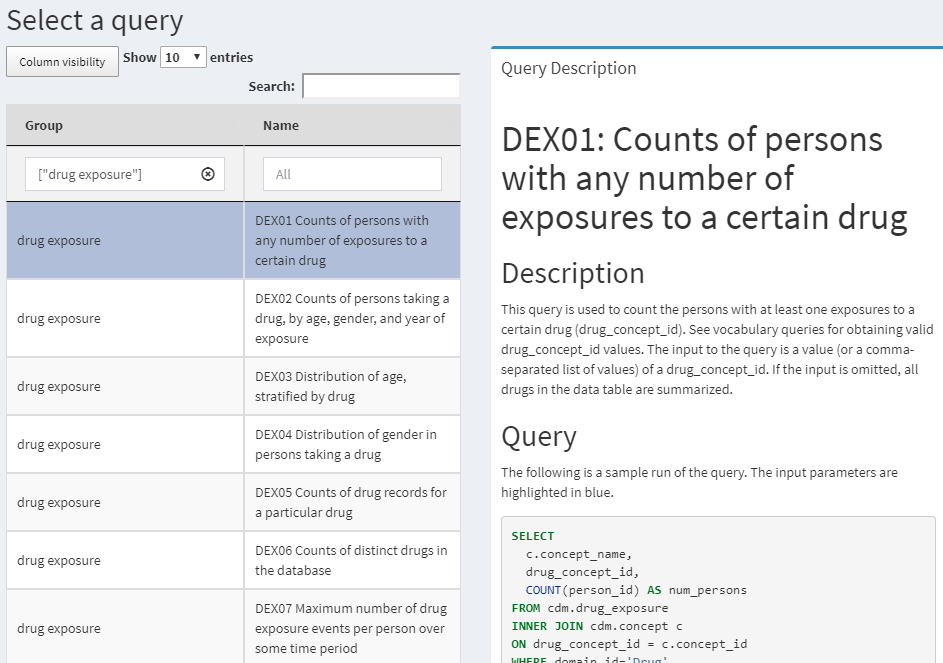
\includegraphics[width=1\linewidth]{images/SqlAndR/queryLibrary} 

}

\caption{QueryLibrary : une bibliothèque de requêtes SQL contre le CDM.}\label{fig:queryLibrary}
\end{figure}

L'objectif de la bibliothèque est d'aider les nouveaux utilisateurs à apprendre à interroger le CDM. Les requêtes dans la bibliothèque ont été examinées et approuvées par la communauté OHDSI. La bibliothèque de requêtes est principalement destinée à des fins de formation, mais elle est également une ressource précieuse pour les utilisateurs expérimentés.

La QueryLibrary utilise SqlRender pour produire les requêtes dans le dialecte SQL de votre choix. Les utilisateurs peuvent également spécifier le schéma de la base de données CDM, le schéma de la base de données de vocabulaire (s'ils sont séparés) et le schéma temporaire d'Oracle (si nécessaire), de sorte que les requêtes seront automatiquement rendues avec ces paramètres.

\section{Concevoir une Étude Simple}\label{concevoir-une-uxe9tude-simple}

\subsection{Définition du Problème}\label{duxe9finition-du-probluxe8me}

L'angio-œdème est un effet secondaire bien connu des inhibiteurs de l'ECA (IECA). \citet{slater_1988} estime que le taux d'incidence de l'angio-œdème dans la première semaine de traitement par IECA est d'un cas pour 3 000 patients par semaine. Ici, nous cherchons à reproduire cette constatation, et à stratifier par âge et sexe. Pour simplifier, nous nous concentrons sur un IECA : le lisinopril. Nous répondons donc à la question

\begin{quote}
Quel est le taux d'angio-œdème dans la première semaine suivant l'initiation du traitement par lisinopril, stratifié par âge et sexe ?
\end{quote}

\subsection{Exposition}\label{exposition}

Nous définirons l'exposition comme la première exposition au lisinopril. Par « première », nous entendons qu'aucune exposition antérieure au lisinopril n'est présente. Nous exigeons 365 jours de temps d'observation continue avant la première exposition.

\subsection{Résultat}\label{ruxe9sultat}

Nous définissons l'angio-œdème comme toute occurrence d'un code de diagnostic d'angio-œdème lors d'une visite en hospitalisation ou aux urgences (ER).

\subsection{Temps à Risque}\label{temps-uxe0-risque}

Nous calculerons le taux d'incidence dans la première semaine suivant l'initiation du traitement, indépendamment de la durée d'exposition des patients pendant la semaine complète.

\section{Implémenter l'Étude en Utilisant SQL et R}\label{impluxe9menter-luxe9tude-en-utilisant-sql-et-r}

Bien que nous ne soyons pas liés aux conventions des outils OHDSI, il est utile de suivre les mêmes principes. Dans ce cas, nous utiliserons SQL pour peupler une table de cohorte, de la même manière que les outils OHDSI. La table COHORT est définie dans le CDM et possède un ensemble prédéfini de champs que nous utiliserons également. Nous devons d'abord créer la table COHORT dans un schéma de base de données où nous avons accès en écriture, ce qui n'est probablement pas le même que le schéma de base de données qui contient les données au format CDM.

\begin{Shaded}
\begin{Highlighting}[]
\FunctionTok{library}\NormalTok{(DatabaseConnector)}
\NormalTok{conn }\OtherTok{\textless{}{-}} \FunctionTok{connect}\NormalTok{(}\AttributeTok{dbms =} \StringTok{"postgresql"}\NormalTok{,}
                \AttributeTok{server =} \StringTok{"localhost/postgres"}\NormalTok{,}
                \AttributeTok{user =} \StringTok{"joe"}\NormalTok{,}
                \AttributeTok{password =} \StringTok{"secret"}\NormalTok{)}
\NormalTok{cdmDbSchema }\OtherTok{\textless{}{-}} \StringTok{"cdm"}
\NormalTok{cohortDbSchema }\OtherTok{\textless{}{-}} \StringTok{"scratch"}
\NormalTok{cohortTable }\OtherTok{\textless{}{-}} \StringTok{"my\_cohorts"}

\NormalTok{sql }\OtherTok{\textless{}{-}} \StringTok{"}
\StringTok{CREATE TABLE @cohort\_db\_schema.@cohort\_table (}
\StringTok{  cohort\_definition\_id INT,}
\StringTok{  cohort\_start\_date DATE,}
\StringTok{  cohort\_end\_date DATE,}
\StringTok{  subject\_id BIGINT}
\StringTok{);}
\StringTok{"}
\FunctionTok{renderTranslateExecuteSql}\NormalTok{(conn, sql,}
                          \AttributeTok{cohort\_db\_schema =}\NormalTok{ cohortDbSchema,}
                          \AttributeTok{cohort\_table =}\NormalTok{ cohortTable)}
\end{Highlighting}
\end{Shaded}

Ici, nous avons paramétré le schéma de base de données et les noms de table, afin de pouvoir les adapter facilement à différents environnements. Le résultat est une table vide sur le serveur de base de données.

\subsection{Cohorte d'Exposition}\label{cohorte-dexposition}

Ensuite, nous créons notre cohorte d'exposition et l'insérons dans notre table COHORT :

\begin{Shaded}
\begin{Highlighting}[]
\NormalTok{sql }\OtherTok{\textless{}{-}} \StringTok{"}
\StringTok{INSERT INTO @cohort\_db\_schema.@cohort\_table (}
\StringTok{  cohort\_definition\_id,}
\StringTok{  cohort\_start\_date,}
\StringTok{  cohort\_end\_date,}
\StringTok{  subject\_id}
\StringTok{)}
\StringTok{SELECT 1 AS cohort\_definition\_id,}
\StringTok{  cohort\_start\_date,}
\StringTok{  cohort\_end\_date,}
\StringTok{  subject\_id}
\StringTok{FROM (}
\StringTok{  SELECT drug\_era\_start\_date AS cohort\_start\_date,}
\StringTok{    drug\_era\_end\_date AS cohort\_end\_date,}
\StringTok{    person\_id AS subject\_id}
\StringTok{  FROM (}
\StringTok{    SELECT drug\_era\_start\_date,}
\StringTok{      drug\_era\_end\_date,}
\StringTok{      person\_id,}
\StringTok{      ROW\_NUMBER() OVER (}
\StringTok{        PARTITION BY person\_id}
\StringTok{            ORDER BY drug\_era\_start\_date}
\StringTok{      ) order\_nr}
\StringTok{    FROM @cdm\_db\_schema.drug\_era}
\StringTok{    WHERE drug\_concept\_id = 1308216 {-}{-} Lisinopril}
\StringTok{  ) ordered\_exposures}
\StringTok{  WHERE order\_nr = 1}
\StringTok{) first\_era}
\StringTok{INNER JOIN @cdm\_db\_schema.observation\_period}
\StringTok{  ON subject\_id = person\_id}
\StringTok{    AND observation\_period\_start\_date \textless{} cohort\_start\_date}
\StringTok{    AND observation\_period\_end\_date \textgreater{} cohort\_start\_date}
\StringTok{WHERE DATEDIFF(DAY,}
\StringTok{               observation\_period\_start\_date,}
\StringTok{               cohort\_start\_date) \textgreater{}= 365;}
\StringTok{"}

\FunctionTok{renderTranslateExecuteSql}\NormalTok{(conn, sql,}
                          \AttributeTok{cohort\_db\_schema =}\NormalTok{ cohortDbSchema,}
                          \AttributeTok{cohort\_table =}\NormalTok{ cohortTable,}
                          \AttributeTok{cdm\_db\_schema =}\NormalTok{ cdmDbSchema)}
\end{Highlighting}
\end{Shaded}

Ici, nous utilisons la table DRUG\_ERA, une table standard dans le CDM automatiquement dérivée de la table DRUG\_EXPOSURE. La table DRUG\_ERA contient des ères d'exposition continue au niveau de l'ingrédient. Nous pouvons ainsi rechercher le lisinopril, et cela identifiera automatiquement toutes les expositions aux médicaments contenant du lisinopril. Nous prenons la première exposition au médicament par personne, puis nous joignons cela à la table OBSERVATION\_PERIOD. Étant donné qu'une personne peut avoir plusieurs périodes d'observation, nous devons nous assurer que nous ne joignons que la période contenant l'exposition au médicament. Nous exigeons ensuite au moins 365 jours entre la OBSERVATION\_PERIOD\_START\_DATE et la COHORT\_START\_DATE.

\subsection{Cohorte de Résultat}\label{cohorte-de-ruxe9sultat}

Enfin, nous devons créer notre cohorte de résultat :

\begin{Shaded}
\begin{Highlighting}[]
\NormalTok{sql }\OtherTok{\textless{}{-}} \StringTok{"}
\StringTok{INSERT INTO @cohort\_db\_schema.@cohort\_table (}
\StringTok{ cohort\_definition\_id,}
\StringTok{ cohort\_start\_date,}
\StringTok{ cohort\_end\_date,}
\StringTok{subject\_id}
\StringTok{)}
\StringTok{SELECT 2 AS cohort\_definition\_id,}
\StringTok{  cohort\_start\_date,}
\StringTok{  cohort\_end\_date,}
\StringTok{  subject\_id}
\StringTok{FROM (}
\StringTok{  SELECT DISTINCT person\_id AS subject\_id,}
\StringTok{    condition\_start\_date AS cohort\_start\_date,}
\StringTok{    condition\_end\_date AS cohort\_end\_date}
\StringTok{  FROM @cdm\_db\_schema.condition\_occurrence}
\StringTok{  INNER JOIN @cdm\_db\_schema.concept\_ancestor}
\StringTok{    ON condition\_concept\_id = descendant\_concept\_id}
\StringTok{  WHERE ancestor\_concept\_id = 432791 {-}{-} Angioedema}
\StringTok{) distinct\_occurrence}
\StringTok{INNER JOIN @cdm\_db\_schema.visit\_occurrence}
\StringTok{  ON subject\_id = person\_id}
\StringTok{  AND visit\_start\_date \textless{}= cohort\_start\_date}
\StringTok{  AND visit\_end\_date \textgreater{}= cohort\_start\_date}
\StringTok{WHERE visit\_concept\_id IN (262, 9203,}
\StringTok{    9201) {-}{-} Inpatient or ER;}
\StringTok{"}

\FunctionTok{renderTranslateExecuteSql}\NormalTok{(conn, sql,}
                          \AttributeTok{cohort\_db\_schema =}\NormalTok{ cohortDbSchema,}
                          \AttributeTok{cohort\_table =}\NormalTok{ cohortTable,}
                          \AttributeTok{cdm\_db\_schema =}\NormalTok{ cdmDbSchema)}
\end{Highlighting}
\end{Shaded}

Ici, nous joignons la table CONDITION\_OCCURRENCE à la table CONCEPT\_ANCESTOR pour trouver toutes les occurrences d'angioedème ou de ses descendants. Nous utilisons DISTINCT pour nous assurer de ne sélectionner qu'un seul enregistrement par jour, car nous pensons que plusieurs diagnostics d'angioedème le même jour sont plus susceptibles d'être la même occurrence plutôt que plusieurs événements distincts d'angioedème. Nous joignons ces occurrences à la table VISIT\_OCCURRENCE pour nous assurer que le diagnostic a été fait en milieu hospitalier ou aux urgences.

\subsection{Calcul du Taux d'Incidence}\label{calcul-du-taux-dincidence}

Maintenant que nos cohortes sont en place, nous pouvons calculer le taux d'incidence, stratifié par âge et sexe :

\begin{Shaded}
\begin{Highlighting}[]
\NormalTok{sql }\OtherTok{\textless{}{-}} \StringTok{"}
\StringTok{WITH tar AS (}
\StringTok{  SELECT concept\_name AS gender,}
\StringTok{    FLOOR((YEAR(cohort\_start\_date) {-}}
\StringTok{          year\_of\_birth) / 10) AS age,}
\StringTok{    subject\_id,}
\StringTok{    cohort\_start\_date,}
\StringTok{    CASE WHEN DATEADD(DAY, 7, cohort\_start\_date) \textgreater{}}
\StringTok{      observation\_period\_end\_date}
\StringTok{    THEN observation\_period\_end\_date}
\StringTok{    ELSE DATEADD(DAY, 7, cohort\_start\_date)}
\StringTok{    END AS cohort\_end\_date}
\StringTok{  FROM @cohort\_db\_schema.@cohort\_table}
\StringTok{  INNER JOIN @cdm\_db\_schema.observation\_period}
\StringTok{    ON subject\_id = observation\_period.person\_id}
\StringTok{      AND observation\_period\_start\_date \textless{} cohort\_start\_date}
\StringTok{      AND observation\_period\_end\_date \textgreater{} cohort\_start\_date}
\StringTok{  INNER JOIN @cdm\_db\_schema.person}
\StringTok{    ON subject\_id = person.person\_id}
\StringTok{  INNER JOIN @cdm\_db\_schema.concept}
\StringTok{    ON gender\_concept\_id = concept\_id}
\StringTok{  WHERE cohort\_definition\_id = 1 {-}{-} Exposure}
\StringTok{)}
\StringTok{SELECT days.gender,}
\StringTok{    days.age,}
\StringTok{    days,}
\StringTok{    CASE WHEN events IS NULL THEN 0 ELSE events END AS events}
\StringTok{FROM (}
\StringTok{  SELECT gender,}
\StringTok{    age,}
\StringTok{    SUM(DATEDIFF(DAY, cohort\_start\_date,}
\StringTok{      cohort\_end\_date)) AS days}
\StringTok{  FROM tar}
\StringTok{  GROUP BY gender,}
\StringTok{    age}
\StringTok{) days}
\StringTok{LEFT JOIN (}
\StringTok{  SELECT gender,}
\StringTok{      age,}
\StringTok{      COUNT(*) AS events}
\StringTok{  FROM tar}
\StringTok{  INNER JOIN @cohort\_db\_schema.@cohort\_table angioedema}
\StringTok{    ON tar.subject\_id = angioedema.subject\_id}
\StringTok{      AND tar.cohort\_start\_date \textless{}= angioedema.cohort\_start\_date}
\StringTok{      AND tar.cohort\_end\_date \textgreater{}= angioedema.cohort\_start\_date}
\StringTok{  WHERE cohort\_definition\_id = 2 {-}{-} Outcome}
\StringTok{  GROUP BY gender,}
\StringTok{    age}
\StringTok{) events}
\StringTok{ON days.gender = events.gender}
\StringTok{  AND days.age = events.age;}
\StringTok{"}

\NormalTok{results }\OtherTok{\textless{}{-}} \FunctionTok{renderTranslateQuerySql}\NormalTok{(conn, sql,}
                                   \AttributeTok{cohort\_db\_schema =}\NormalTok{ cohortDbSchema,}
                                   \AttributeTok{cohort\_table =}\NormalTok{ cohortTable,}
                                   \AttributeTok{cdm\_db\_schema =}\NormalTok{ cdmDbSchema,}
                                   \AttributeTok{snakeCaseToCamelCase =} \ConstantTok{TRUE}\NormalTok{)}
\end{Highlighting}
\end{Shaded}

Nous créons d'abord ``tar,'' un CTE qui contient toutes les expositions avec le temps à risque approprié. Notez que nous tronquons le temps à risque à la OBSERVATION\_PERIOD\_END\_DATE. Nous calculons également l'âge par tranche de 10 ans et identifions le genre. L'avantage d'utiliser un CTE est que nous pouvons utiliser le même ensemble de résultats intermédiaires plusieurs fois dans une requête. Dans ce cas, nous l'utilisons pour compter la quantité totale de temps à risque, ainsi que le nombre d'événements d'angioedème qui se produisent pendant le temps à risque.

Nous utilisons \texttt{snakeCaseToCamelCase\ =\ TRUE} car en SQL, nous avons tendance à utiliser snake\_case pour les noms de champs (parce que SQL est insensible à la casse), tandis qu'en R nous avons tendance à utiliser camelCase (parce que R est sensible à la casse). Les noms de colonnes du data frame \texttt{results} seront maintenant en camelCase.

Avec l'aide du package ggplot2, nous pouvons facilement tracer nos résultats :

\begin{Shaded}
\begin{Highlighting}[]
\CommentTok{\# Calculer le taux d\textquotesingle{}incidence (IR) :}
\NormalTok{results}\SpecialCharTok{$}\NormalTok{ir }\OtherTok{\textless{}{-}} \DecValTok{1000} \SpecialCharTok{*}\NormalTok{ results}\SpecialCharTok{$}\NormalTok{events }\SpecialCharTok{/}\NormalTok{ results}\SpecialCharTok{$}\NormalTok{days }\SpecialCharTok{/} \DecValTok{7}

\CommentTok{\# Corriger l\textquotesingle{}échelle d\textquotesingle{}âge:}
\NormalTok{results}\SpecialCharTok{$}\NormalTok{age }\OtherTok{\textless{}{-}}\NormalTok{ results}\SpecialCharTok{$}\NormalTok{age }\SpecialCharTok{*} \DecValTok{10}

\FunctionTok{library}\NormalTok{(ggplot2)}
\FunctionTok{ggplot}\NormalTok{(results, }\FunctionTok{aes}\NormalTok{(}\AttributeTok{x =}\NormalTok{ age, }\AttributeTok{y =}\NormalTok{ ir, }\AttributeTok{group =}\NormalTok{ gender, }\AttributeTok{color =}\NormalTok{ gender)) }\SpecialCharTok{+}
  \FunctionTok{geom\_line}\NormalTok{() }\SpecialCharTok{+}
  \FunctionTok{xlab}\NormalTok{(}\StringTok{"Âge"}\NormalTok{) }\SpecialCharTok{+}
  \FunctionTok{ylab}\NormalTok{(}\StringTok{"Incidence (pour 1 000 patients{-}semaines)"}\NormalTok{)}
\end{Highlighting}
\end{Shaded}

\begin{center}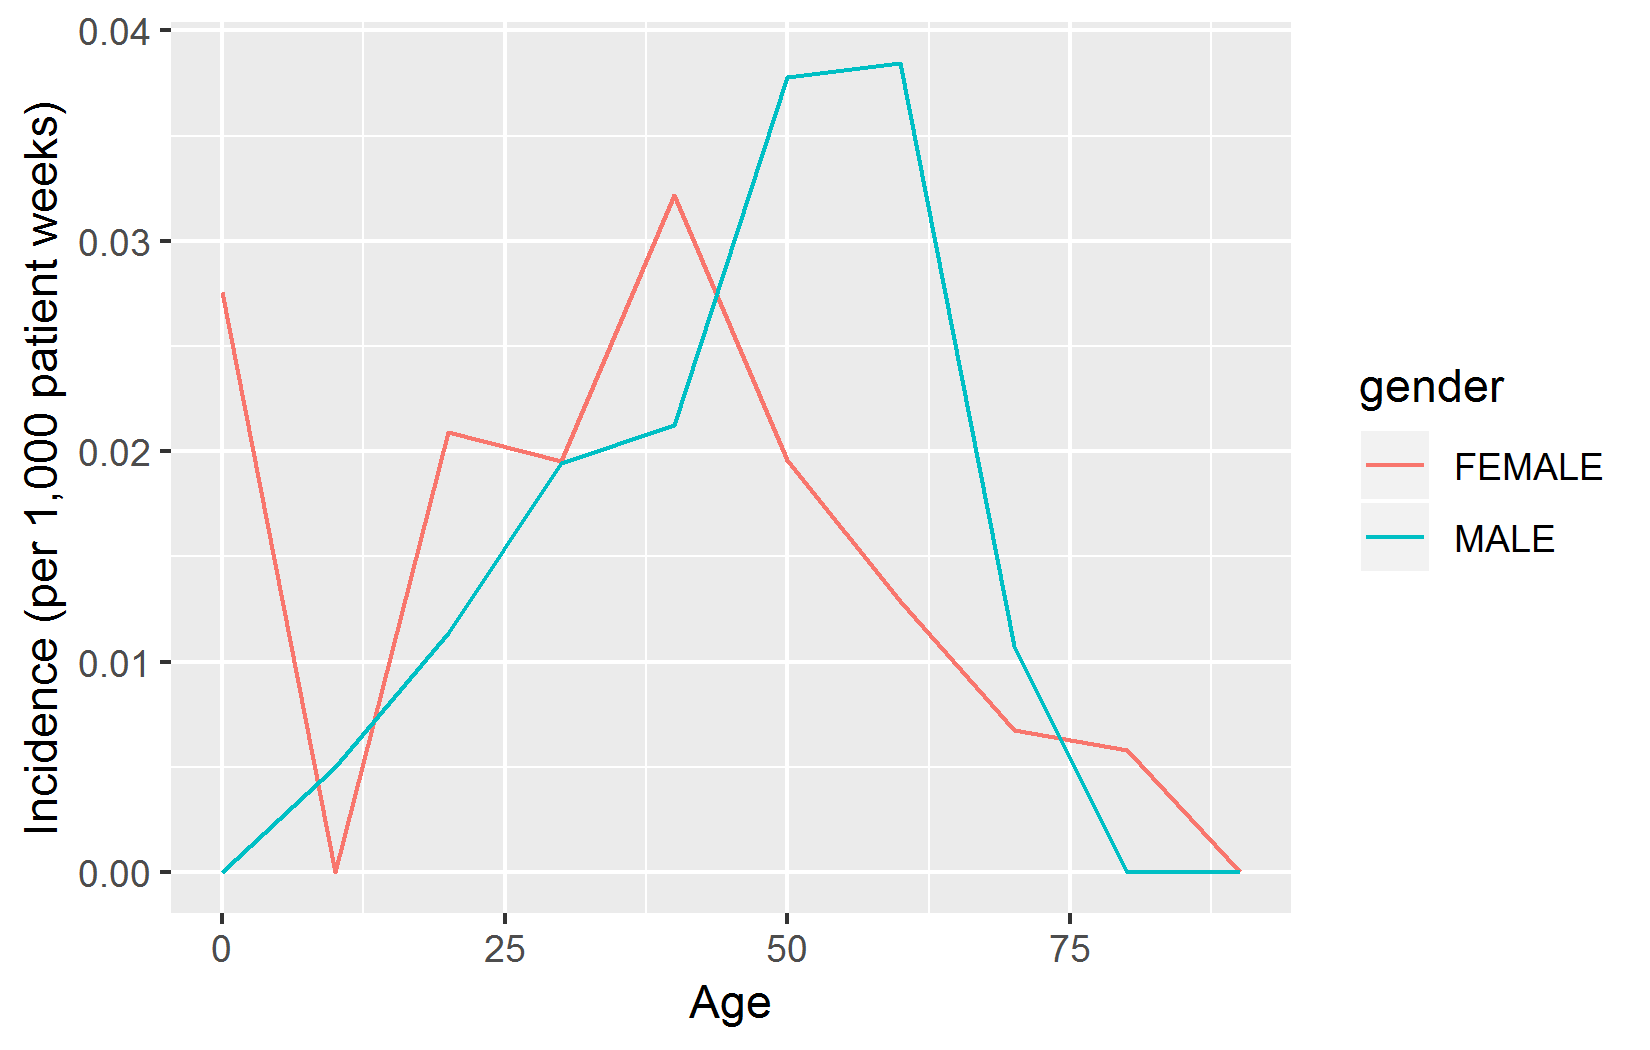
\includegraphics[width=0.8\linewidth]{images/SqlAndR/ir} \end{center}

\subsection{Nettoyage}\label{nettoyage}

N'oubliez pas de nettoyer la table que nous avons créée et de fermer la connexion :

\begin{Shaded}
\begin{Highlighting}[]
\NormalTok{sql }\OtherTok{\textless{}{-}} \StringTok{"}
\StringTok{TRUNCATE TABLE @cohort\_db\_schema.@cohort\_table;}
\StringTok{DROP TABLE @cohort\_db\_schema.@cohort\_table;}
\StringTok{"}
\FunctionTok{renderTranslateExecuteSql}\NormalTok{(conn, sql,}
                          \AttributeTok{cohort\_db\_schema =}\NormalTok{ cohortDbSchema,}
                          \AttributeTok{cohort\_table =}\NormalTok{ cohortTable)}

\FunctionTok{disconnect}\NormalTok{(conn)}
\end{Highlighting}
\end{Shaded}

\subsection{Compatibilité}\label{compatibilituxe9}

Parce que nous utilisons OHDSI SQL avec DatabaseConnector et SqlRender partout, le code que nous avons examiné ici fonctionnera sur toutes les plateformes de base de données prises en charge par OHDSI.

Notez que, à des fins de démonstration, nous avons choisi de créer nos cohortes en utilisant du SQL écrit à la main. Il aurait probablement été plus pratique de construire la définition de la cohorte dans ATLAS, et d'utiliser le SQL généré par ATLAS pour instancier les cohortes. ATLAS produit également du SQL OHDSI et peut donc facilement être utilisé avec SqlRender et DatabaseConnector.

\section{Résumé}\label{ruxe9sumuxe9-7}

\begin{rmdsummary}
\begin{itemize}
\item
  \textbf{SQL} (Structured Query Language) est un langage standard pour interroger les bases de données, y compris celles qui sont conformes au Common Data Model (CDM).
\item
  Différentes plateformes de bases de données ont des dialectes SQL différents et nécessitent des outils différents pour les interroger.
\item
  Les packages R \textbf{SqlRender} et \textbf{DatabaseConnector} fournissent un moyen unifié pour interroger les données dans le CDM, permettant au même code d'analyse de s'exécuter dans différents environnements sans modification.
\item
  En utilisant R et SQL ensemble, nous pouvons mettre en œuvre des analyses personnalisées qui ne sont pas prises en charge par les outils OHDSI.
\item
  La \textbf{QueryLibrary} fournit une collection de requêtes SQL réutilisables pour le CDM.
\end{itemize}
\end{rmdsummary}

\section{Exercices}\label{exercices-4}

\subsubsection*{Prérequis}\label{pruxe9requis-3}
\addcontentsline{toc}{subsubsection}{Prérequis}

Pour ces exercices, nous supposons que R, R-Studio et Java ont été installés comme décrit dans la section \ref{installR}. Les packages \href{https://ohdsi.github.io/SqlRender/}{SqlRender}, \href{https://ohdsi.github.io/DatabaseConnector/}{DatabaseConnector} et \href{https://ohdsi.github.io/Eunomia/}{Eunomia} sont également nécessaires et peuvent être installés en utilisant :

\begin{Shaded}
\begin{Highlighting}[]
\FunctionTok{install.packages}\NormalTok{(}\FunctionTok{c}\NormalTok{(}\StringTok{"SqlRender"}\NormalTok{, }\StringTok{"DatabaseConnector"}\NormalTok{, }\StringTok{"remotes"}\NormalTok{))}
\NormalTok{remotes}\SpecialCharTok{::}\FunctionTok{install\_github}\NormalTok{(}\StringTok{"ohdsi/Eunomia"}\NormalTok{, }\AttributeTok{ref =} \StringTok{"v1.0.0"}\NormalTok{)}
\end{Highlighting}
\end{Shaded}

Le package Eunomia fournit un ensemble de données simulé dans le CDM qui s'exécute au sein de votre session R locale. Les détails de connexion peuvent être obtenus en utilisant :

\begin{Shaded}
\begin{Highlighting}[]
\NormalTok{connectionDetails }\OtherTok{\textless{}{-}}\NormalTok{ Eunomia}\SpecialCharTok{::}\FunctionTok{getEunomiaConnectionDetails}\NormalTok{()}
\end{Highlighting}
\end{Shaded}

Le schéma de la base de données CDM est ``main''.

\begin{exercise}
\protect\hypertarget{exr:exercisePeopleCount}{}\label{exr:exercisePeopleCount}En utilisant SQL et R, calculez combien de personnes se trouvent dans la base de données.
\end{exercise}

\begin{exercise}
\protect\hypertarget{exr:exerciseCelecoxibUsers}{}\label{exr:exerciseCelecoxibUsers}En utilisant SQL et R, calculez combien de personnes ont au moins une prescription de célécoxib.
\end{exercise}

\begin{exercise}
\protect\hypertarget{exr:exerciseGiBleedsDuringCelecoxib}{}\label{exr:exerciseGiBleedsDuringCelecoxib}En utilisant SQL et R, calculez combien de diagnostics d'hémorragie gastro-intestinale surviennent pendant l'exposition au célécoxib. (Indice : l'ID de concept pour l'hémorragie gastro-intestinale est \href{http://athena.ohdsi.org/search-terms/terms/192671}{192671}.)
\end{exercise}

Les réponses suggérées se trouvent dans l'Appendice \ref{SqlAndRanswers}.

\chapter{Définir des Cohortes}\label{Cohorts}

\emph{Chef de chapitre : Kristin Kostka}

Les données de santé observationnelles, également appelées \emph{données du monde réel}, sont les données liées à l'état de santé des patients et/ou à la prestation des soins de santé, recueillies de manière routinière à partir de diverses sources. En tant que telles, les gestionnaires de données OHDSI (collaborateurs OHDSI qui maintiennent les données dans le CDM pour leurs sites) peuvent capturer des données provenant de plusieurs sources, y compris les dossiers de santé électroniques (DSE), les réclamations d'assurance santé et les activités de facturation, les registres de produits et de maladies, les données générées par les patients y compris en milieu domestique, et les données recueillies à partir d'autres sources pouvant fournir des informations sur l'état de santé, telles que les appareils mobiles. Comme ces données n'ont pas été collectées à des fins de recherche, elles peuvent ne pas capturer explicitement les éléments de données cliniques qui nous intéressent.

Par exemple, une base de données de réclamations d'assurance maladie est conçue pour capturer tous les soins fournis pour une certaine condition (par exemple, l'angio-œdème) afin que les coûts associés puissent être remboursés de manière appropriée, et les informations sur la condition réelle ne sont capturées que dans le cadre de cet objectif. Si nous souhaitons utiliser de telles données observationnelles à des fins de recherche, nous devrons souvent rédiger une logique utilisant \emph{ce qui est capturé dans les données} pour en déduire \emph{ce qui nous intéresse réellement}. En d'autres termes, nous devons souvent créer une cohorte en utilisant une certaine définition de la façon dont un événement clinique se manifeste. Ainsi, si nous voulons identifier les événements d'angio-œdème dans une base de données de réclamations d'assurance, nous pouvons définir une logique exigeant un code de diagnostic d'angio-œdème enregistré dans un cadre de salle d'urgence, pour distinguer des réclamations qui décrivent simplement les soins de suivi pour une occurrence passée d'angio-œdème. Des considérations similaires peuvent s'appliquer aux données capturées lors d'interactions de soins de santé de routine enregistrées dans un DSE. Étant donné que les données sont utilisées à des fins secondaires, nous devons être conscients de ce que chaque base de données a été initialement conçue pour faire. Chaque fois que nous concevons une étude, nous devons réfléchir aux nuances de la façon dont notre cohorte existe dans divers contextes de soins de santé.

Le chapitre sert à expliquer ce que signifie créer et partager des définitions de cohortes, les méthodes de développement des cohortes, et comment construire vos propres cohortes en utilisant ATLAS ou SQL.

\section{Qu'est-ce qu'une Cohorte ?}\label{quest-ce-quune-cohorte}

Dans les recherches OHDSI, nous définissons une cohorte comme un ensemble de personnes qui satisfont un ou plusieurs critères d'inclusion pendant une durée de temps. Le terme cohorte est souvent utilisé de manière interchangeable avec le terme \emph{phénotype}. Les cohortes sont utilisées dans tous les outils analytiques OHDSI et les études en réseau comme les blocs de construction primaires pour exécuter une question de recherche. Par exemple, dans une étude visant à prédire le risque d'angio-œdème dans un groupe de personnes commençant des inhibiteurs de l'enzyme de conversion de l'angiotensine (ECA), nous définissons deux cohortes : la cohorte d'issue (angio-œdème), et la cohorte cible (personnes commençant des inhibiteurs ECA). Un aspect important des cohortes dans OHDSI est qu'elles sont généralement définies indépendamment des autres cohortes de l'étude, permettant ainsi la réutilisation. Par exemple, dans notre exemple, la cohorte d'angio-œdème identifierait tous les événements d'angio-œdème dans la population, y compris ceux en dehors de la population cible. Nos outils analytiques prendront l'intersection de ces deux cohortes lorsqu'il le faut lors de l'analyse. L'avantage de cela est que la même définition de la cohorte d'angio-œdème peut désormais également être utilisée dans d'autres analyses, par exemple une étude d'estimation comparant les inhibiteurs ECA à une autre exposition. Les définitions de cohortes peuvent varier d'une étude à l'autre en fonction de la question de recherche d'intérêt.

\begin{rmdimportant}
Une cohorte est un ensemble de personnes qui satisfont un ou plusieurs critères d'inclusion pendant une durée de temps.
\end{rmdimportant}

\index{cohorte} \index{définition de cohorte}
Il est important de comprendre que cette définition d'une cohorte utilisée dans OHDSI pourrait différer de celle utilisée par d'autres dans le domaine. Par exemple, dans de nombreux manuscrits scientifiques évalués par des pairs, une cohorte est suggérée être analogue à un ensemble de codes spécifiques cliniques (par exemple, ICD-9/ICD-10, NDC, HCPCS, etc.). Bien que les ensembles de codes soient une pièce importante dans l'assemblage d'une cohorte, une cohorte n'est pas définie par un ensemble de codes. Une cohorte nécessite une logique spécifique pour utiliser l'ensemble de codes pour les critères (par exemple, est-ce la première occurrence du code ICD-9/ICD-10 ? toute occurrence ?). Une cohorte bien définie spécifie comment un patient entre dans une cohorte et comment un patient sort d'une cohorte.
\index{ensemble de codes}

\index{phénotype}
Il y a des nuances uniques à l'utilisation de la définition d'une cohorte par OHDSI, notamment :

\begin{itemize}
\tightlist
\item
  Une personne peut appartenir à plusieurs cohortes
\item
  Une personne peut appartenir à la même cohorte pendant plusieurs périodes différentes
\item
  Une personne ne peut pas appartenir à la même cohorte plusieurs fois pendant la même période de temps
\item
  Une cohorte peut avoir zéro ou plusieurs membres
\end{itemize}

Il existe deux approches principales pour construire une cohorte :

\begin{enumerate}
\def\labelenumi{\arabic{enumi}.}
\tightlist
\item
  \textbf{Définitions de cohortes basées sur des règles} utilisent des règles explicites pour décrire quand un patient fait partie de la cohorte. La définition de ces règles repose généralement fortement sur l'expertise dans le domaine thérapeutique de la personne qui conçoit la cohorte pour utiliser ses connaissances du domaine thérapeutique d'intérêt pour construire des règles pour les critères d'inclusion de la cohorte.
\item
  \textbf{Définitions de cohortes probabilistes} utilisent un modèle probabiliste pour calculer une probabilité comprise entre 0 et 100 \% que le patient fasse partie de la cohorte. Cette probabilité peut être transformée en une classification oui-non en utilisant un certain seuil, ou dans certains plans d'études peut être utilisée telle quelle. Le modèle probabiliste est généralement entraîné à l'aide de l'apprentissage automatique (par exemple, la régression logistique) sur certaines données d'exemple pour identifier automatiquement les caractéristiques pertinentes des patients qui sont prédictives.
\end{enumerate}

Les sections suivantes discuteront de ces approches plus en détail.
\#\# Définition de Cohorte Basée sur des Règles

Une définition de cohorte basée sur des règles commence par l'énoncé explicite d'un ou plusieurs critères d'inclusion (par exemple « personnes atteintes d'œdème de Quincke ») sur une durée spécifique (par exemple « ayant développé cette condition au cours des 6 derniers mois »). \index{cohort!rule-based design}

Les composants standards que nous utilisons pour assembler ces critères sont :

\begin{itemize}
\item
  \textbf{Domaine} : Le(s) domaine(s) du CDM où les données sont stockées (par exemple ``Procédure'', ``Exposition aux Médicaments'') définissent le type d'information clinique et les concepts admissibles qui peuvent être représentés dans cette table CDM. Les domaines sont abordés plus en détail dans la Section \ref{domains}.
\item
  \textbf{Ensemble de concepts} : Une expression agnostique aux données qui définit un ou plusieurs Concepts Standard englobant l'entité clinique d'intérêt. Ces ensembles de concepts sont interopérables entre différentes données de santé observationnelles car ils représentent les termes standards auxquels l'entité clinique est mappée dans le Vocabulaire. Les ensembles de concepts sont discutés dans la Section \ref{conceptSets}.
\item
  \textbf{Attribut spécifique au domaine} : Attributs supplémentaires liés à l'entité clinique d'intérêt (par exemple, DAYS\_SUPPLY pour un DRUG\_EXPOSURE, ou VALUE\_AS\_NUMBER ou RANGE\_HIGH pour une MEASUREMENT).
\item
  \textbf{Logique temporelle} : Les intervalles de temps dans lesquels la relation entre un critère d'inclusion et un événement est évaluée (par exemple, la condition indiquée doit se produire dans les 365 jours précédant ou lors du début de l'exposition).
\end{itemize}

Lors de la construction de votre définition de cohorte, il peut être utile de penser aux Domaines comme des blocs de construction (voir Figure \ref{fig:cohortLegos}) représentant les attributs de cohorte. Si vous êtes confus quant au contenu admissible dans chaque domaine, vous pouvez toujours vous référer au chapitre du Modèle de Données Communs (Chapitre \ref{CommonDataModel}) pour obtenir de l'aide.

\begin{figure}

{\centering 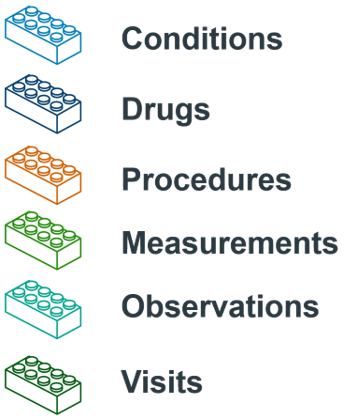
\includegraphics[width=0.5\linewidth]{images/Cohorts/cohort-legos} 

}

\caption{Building Blocks of Cohort definitions.}\label{fig:cohortLegos}
\end{figure}

Lors de la création d'une définition de cohorte, vous devez vous poser les questions suivantes :

\begin{itemize}
\tightlist
\item
  \emph{Quel événement initial définit la date d'entrée dans la cohorte ?}
\item
  \emph{Quels critères d'inclusion sont appliqués aux événements initiaux ?}
\item
  \emph{Qu'est-ce qui définit la date de sortie de la cohorte ?}
\end{itemize}

\textbf{Événement d'entrée dans la cohorte} : L'événement d'entrée dans la cohorte (événement initial) définit le moment où les personnes entrent dans la cohorte, appelé la \textbf{date indice de la cohorte}. Un événement d'entrée de cohorte peut être tout événement enregistré dans le CDM, tel que des expositions à des médicaments, des conditions, des procédures, des mesures et des visites. Les événements initiaux sont définis par le domaine CDM où les données sont stockées (par exemple PROCEDURE\_OCCURRENCE, DRUG\_EXPOSURE, etc.), les ensembles de concepts construits pour identifier l'activité clinique (par exemple, les codes SNOMED pour les conditions, les codes RxNorm pour les médicaments) ainsi que tout autre attribut spécifique (par exemple, âge à la survenue, premier diagnostic/procédure/ etc., spécifiant la date de début et de fin, spécifiant le type de visite ou de critère, jours de fourniture, etc). L'ensemble des personnes ayant un événement d'entrée est appelé la \textbf{cohorte d'événement initial}. \index{cohort!entry event}

\textbf{Critères d'inclusion} : Les critères d'inclusion sont appliqués à la cohorte d'événement initial pour restreindre davantage l'ensemble des personnes. Chaque critère d'inclusion est défini par le(s) domaine(s) CDM où les données sont stockées, les ensembles de concepts représentant l'activité clinique, les attributs spécifiques au domaine (par exemple, jours de fourniture, type de visite, etc.), et la logique temporelle par rapport à la date indice de la cohorte. Chaque critère d'inclusion peut être évalué pour déterminer l'impact des critères sur l'attrition des personnes de la cohorte d'événement initial. La \textbf{cohorte qualifiante} est définie comme toutes les personnes de la cohorte d'événement initial qui satisfont à tous les critères d'inclusion. \index{cohort!inclusion criteria}

\textbf{Critères de sortie de cohorte} : L'événement de sortie de la cohorte signifie lorsque qu'une personne ne satisfait plus aux critères de la cohorte. La sortie de la cohorte peut être définie de plusieurs manières telles que la fin de la période d'observation, un intervalle de temps fixe par rapport à l'événement d'entrée initial, le dernier événement d'une séquence d'observations connexes (par exemple, exposition médicamenteuse persistante) ou par d'autres censures de la période d'observation. La stratégie de sortie de cohorte aura un impact sur le fait qu'une personne peut appartenir à la cohorte plusieurs fois pendant des intervalles de temps différents. \index{cohort!exit criteria}

\begin{rmdimportant}
Dans les outils OHDSI, il n'y a pas de distinction entre les critères d'inclusion et d'exclusion. Tous les critères sont formulés comme des critères d'inclusion. Par exemple, le critère d'exclusion « Exclure les personnes ayant une hypertension antérieure » peut être formulé comme le critère d'inclusion « Inclure les personnes ayant 0 occurrences d'hypertension antérieure ».
\end{rmdimportant}

\section{Ensembles de Concepts}\label{conceptSets}

\index{concept set}

Un ensemble de concepts est une expression représentant une liste de concepts pouvant être utilisée comme composant réutilisable dans diverses analyses. Il peut être considéré comme un équivalent normalisé et exécutable par ordinateur des listes de codes souvent utilisées dans les études observationnelles. Une expression d'ensemble de concepts se compose d'une liste de concepts avec les attributs suivants :

\begin{itemize}
\tightlist
\item
  \textbf{Exclure} : Exclure ce concept (et chacun de ses descendants si sélectionné) de l'ensemble de concepts.
\item
  \textbf{Descendants} : Considérer non seulement ce concept, mais aussi tous ses descendants.
\item
  \textbf{Cartographié} : Permettre la recherche de concepts non standards.
\end{itemize}

Par exemple, une expression d'ensemble de concepts pourrait contenir deux concepts comme illustré dans le Tableau \ref{tab:conceptSetExpression}. Ici, nous incluons le concept \href{http://athena.ohdsi.org/search-terms/terms/4329847}{4329847} (« Infarctus du myocarde ») et tous ses descendants, mais excluons le concept \href{http://athena.ohdsi.org/search-terms/terms/314666}{314666} (« Ancien infarctus du myocarde ») et tous ses descendants.

Tableau : \label{tab:conceptSetExpression} Un exemple d'expression d'ensemble de concepts.

\begin{longtable}[]{@{}lllll@{}}
\toprule\noalign{}
Id Concept & Nom du Concept & Exclu & Descendants & Cartographié \\
\midrule\noalign{}
\endhead
\bottomrule\noalign{}
\endlastfoot
4329847 & Infarctus du myocarde & NON & OUI & NON \\
314666 & Ancien infarctus du myocarde & OUI & OUI & NON \\
\end{longtable}

Comme montré dans la Figure \ref{fig:conceptSet}, cela inclura « Infarctus du myocarde » et tous ses descendants sauf « Ancien infarctus du myocarde » et ses descendants. Au total, cette expression d'ensemble de concepts implique près d'une centaine de Concepts Standards. Ces Concepts Standards à leur tour reflètent des centaines de codes sources (par exemple, codes CIM-9 et CIM-10) qui peuvent apparaître dans les différentes bases de données.

\begin{figure}

{\centering 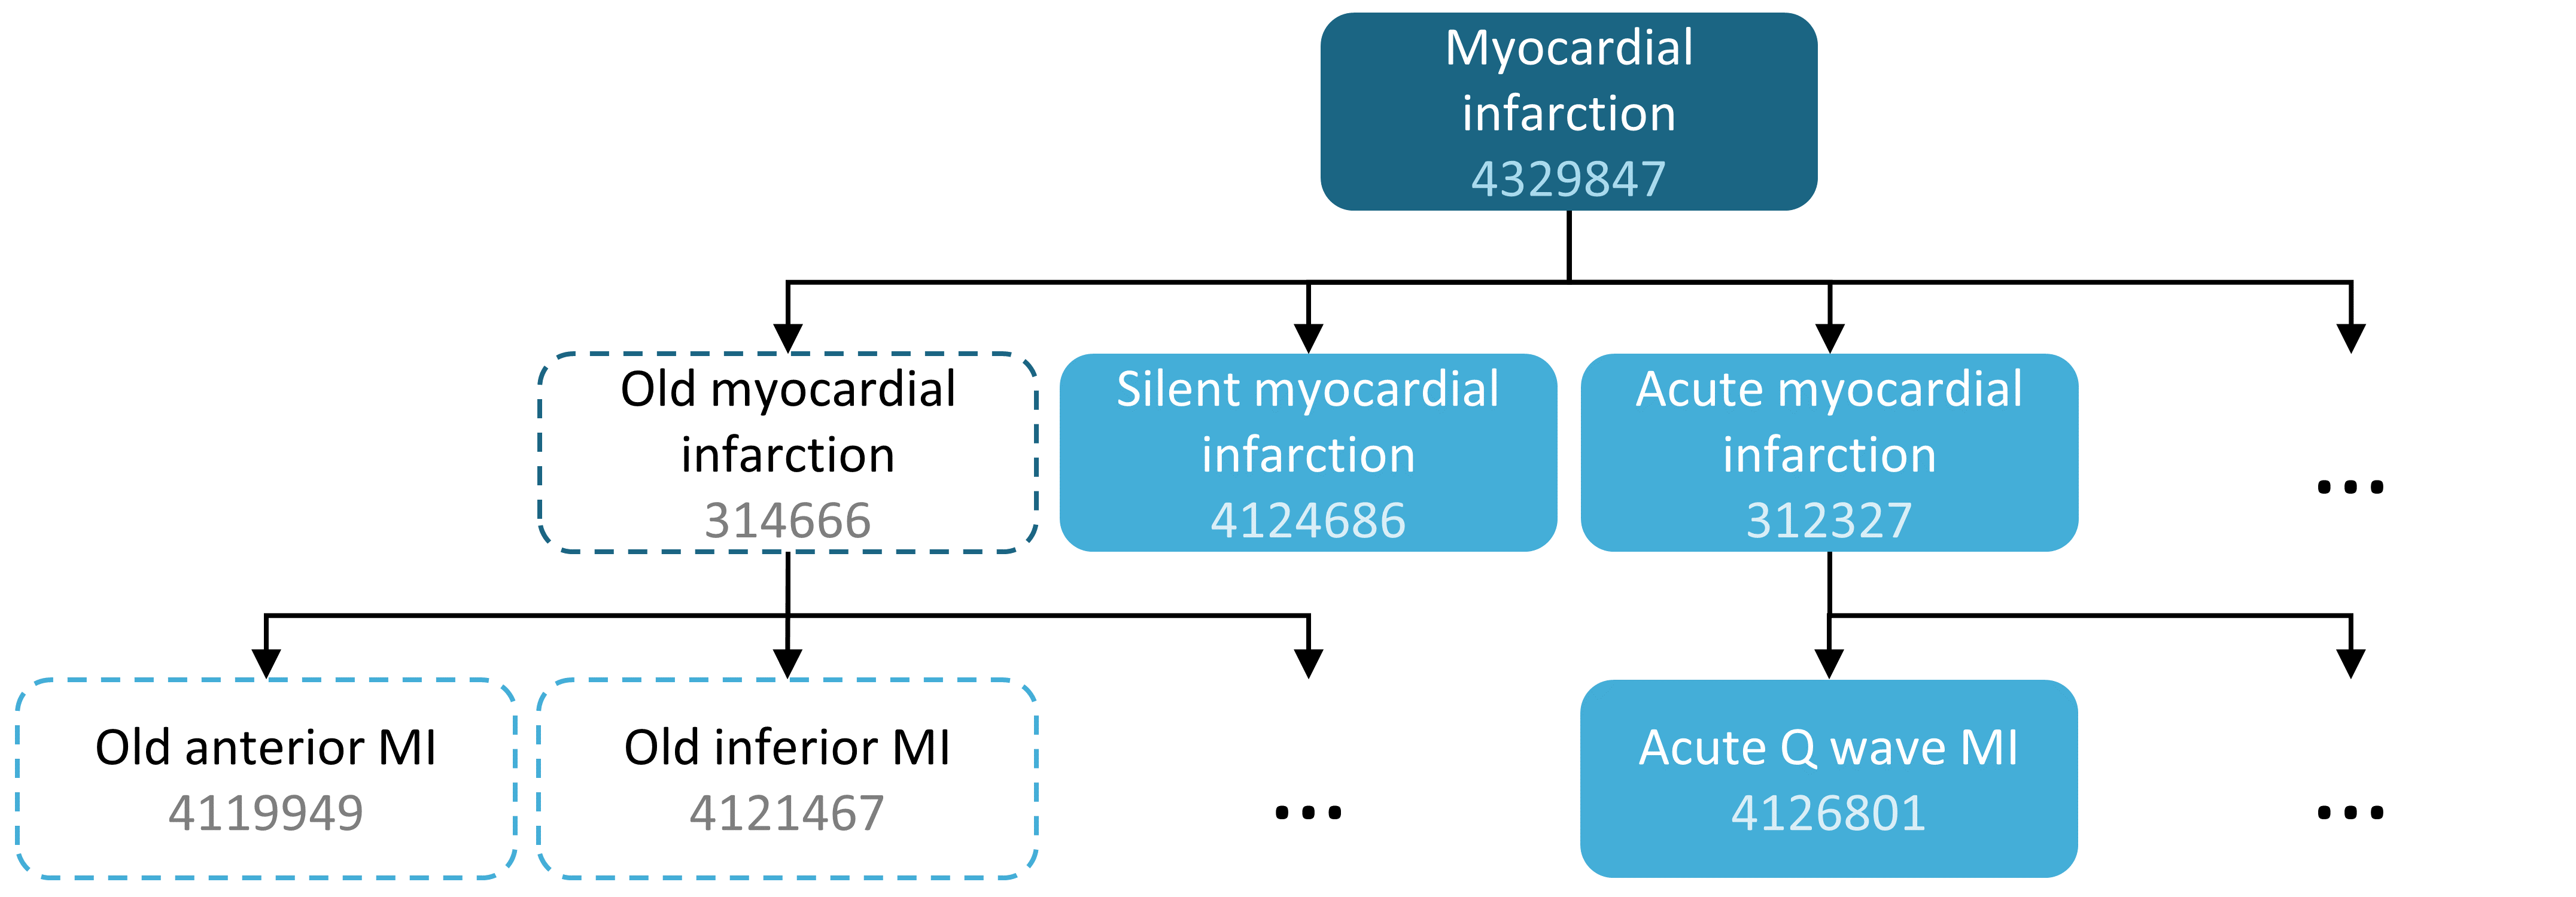
\includegraphics[width=1\linewidth]{images/Cohorts/conceptSet} 

}

\caption{A concept set including "Myocardial infarction" (with descendants), but excluding "Old myocardial infarction" (with descendants).}\label{fig:conceptSet}
\end{figure}

\section{Définitions de Cohorte Probabilistes}\label{duxe9finitions-de-cohorte-probabilistes}

Les définitions de cohorte basées sur des règles sont une méthode populaire pour assembler des définitions de cohorte. Cependant, rassembler le consensus nécessaire d'experts pour créer une cohorte d'étude peut être prohibitif en termes de temps. La conception de cohorte probabiliste est une méthode alternative, pilotée par une machine, pour accélérer la sélection des attributs de cohorte. Dans cette approche, l'apprentissage machine supervisé permet à un algorithme de phénotypage d'apprendre à partir d'un ensemble d'exemples étiquetés (cas) quels attributs contribuent à l'appartenance à la cohorte. Cet algorithme peut ensuite être utilisé pour mieux déterminer les caractéristiques définissant un phénotype et quels compromis se produisent dans la précision globale de l'étude lorsqu'on choisit de modifier les critères de phénotype. \index{cohort!probabilistic design}

Un exemple d'application de cette approche sur les données du CDM est le package R APHRODITE (Automated PHenotype Routine for Observational Definition, Identification, Training and Evaluation)\footnote{\url{https://github.com/OHDSI/Aphrodite}} . Ce package fournit un cadre de construction de cohorte qui combine la capacité d'apprentissage à partir de données imparfaitement étiquetées. \citep{Banda2017APHRODITE} \index{APHRODITE}

\section{Validité de la Définition d'une Cohorte}\label{validituxe9-de-la-duxe9finition-dune-cohorte}

Lorsque vous construisez une cohorte, vous devez considérer ce qui est le plus important pour vous : \emph{trouver tous les patients éligibles ?} ou \emph{obtenir seulement ceux dont vous êtes sûr ?}

Votre stratégie pour construire votre cohorte dépendra de la rigueur clinique de la façon dont votre consensus d'experts définit la maladie. Autrement dit, la bonne conception de la cohorte dépendra de la question que vous tentez de répondre. Vous pouvez choisir de construire une définition de cohorte qui utilise tout ce que vous pouvez obtenir, utilise le plus petit dénominateur commun pour que vous puissiez la partager à travers les sites d'OHDSI ou trouve un compromis entre les deux. En fin de compte, il appartient au chercheur de décider quel seuil de rigueur est nécessaire pour étudier adéquatement la cohorte d'intérêt.

Comme mentionné au début du chapitre, une définition de cohorte est une tentative d'inférer quelque chose que nous aimerions observer à partir des données enregistrées. Cela soulève la question de savoir dans quelle mesure nous avons réussi dans cette tentative. En général, la validation d'une définition de cohorte basée sur des règles ou d'un algorithme probabiliste peut être envisagée comme un test de la cohorte proposée par rapport à une sorte de référence ``gold standard'' (par exemple, une révision manuelle des dossiers des cas). Ceci est discuté en détail dans le Chapitre \ref{ClinicalValidity} (``Validité Clinique'').

\subsection{Bibliothèque de Phénotypes Gold Standard d'OHDSI}\label{bibliothuxe8que-de-phuxe9notypes-gold-standard-dohdsi}

Pour aider la communauté dans l'inventaire et l'évaluation globale des définitions de cohortes et algorithmes existants, le Groupe de Travail de la Bibliothèque de Phénotypes Gold Standard (GSPL) d'OHDSI a été formé. Le but du groupe de travail GSPL est de développer une bibliothèque de phénotypes soutenue par la communauté à partir de méthodes basées sur des règles et probabilistes. La GSPL permet aux membres de la communauté OHDSI de trouver, évaluer et utiliser des définitions de cohortes validées par la communauté pour la recherche et d'autres activités. Ces définitions ``gold standard'' résideront dans une bibliothèque, dont les entrées sont tenues à des normes spécifiques de conception et d'évaluation. Pour des informations supplémentaires relatives à la GSPL, consultez la page du groupe de travail OHDSI.\footnote{\url{https://www.ohdsi.org/web/wiki/doku.php?id=projects:workgroups:gold-library-wg}} Les recherches au sein de ce groupe de travail comprennent APHRODITE \citep{Banda2017APHRODITE} et l'outil PheValuator \citep{Swerdel2019phevaluator}, discutés dans la section précédente, ainsi que le travail effectué pour partager la Bibliothèque des Phénotypes des Dossiers Médicaux Électroniques et de la Génomique \href{https://emerge.mc.vanderbilt.edu/}{eMERGE} \href{https://phekb.org/phenotypes}{Bibliothèque des Phénotypes} à travers le réseau OHDSI \citep{Hripcsak2019eMERGE}. Si la curation des phénotypes vous intéresse, pensez à contribuer à ce groupe de travail. \index{bibliothèque de phénotypes}

\section{Définir une Cohorte pour l'Hypertension}\label{duxe9finir-une-cohorte-pour-lhypertension}

Nous commençons à pratiquer nos compétences en matière de cohorte en assemblant une définition de cohorte en utilisant une approche basée sur des règles. Dans cet exemple, nous voulons trouver les \emph{patients qui initient une monothérapie par inhibiteurs de l'ECA comme traitement de première ligne pour l'hypertension}.

Avec ce contexte en tête, nous allons maintenant construire notre cohorte. Au fur et à mesure de cet exercice, nous approcherons la construction de notre cohorte de manière similaire à un diagramme d'attrition standard. La Figure \ref{fig:CohortPractice} montre le cadre logique pour la manière dont nous voulons construire cette cohorte.

\begin{figure}

{\centering 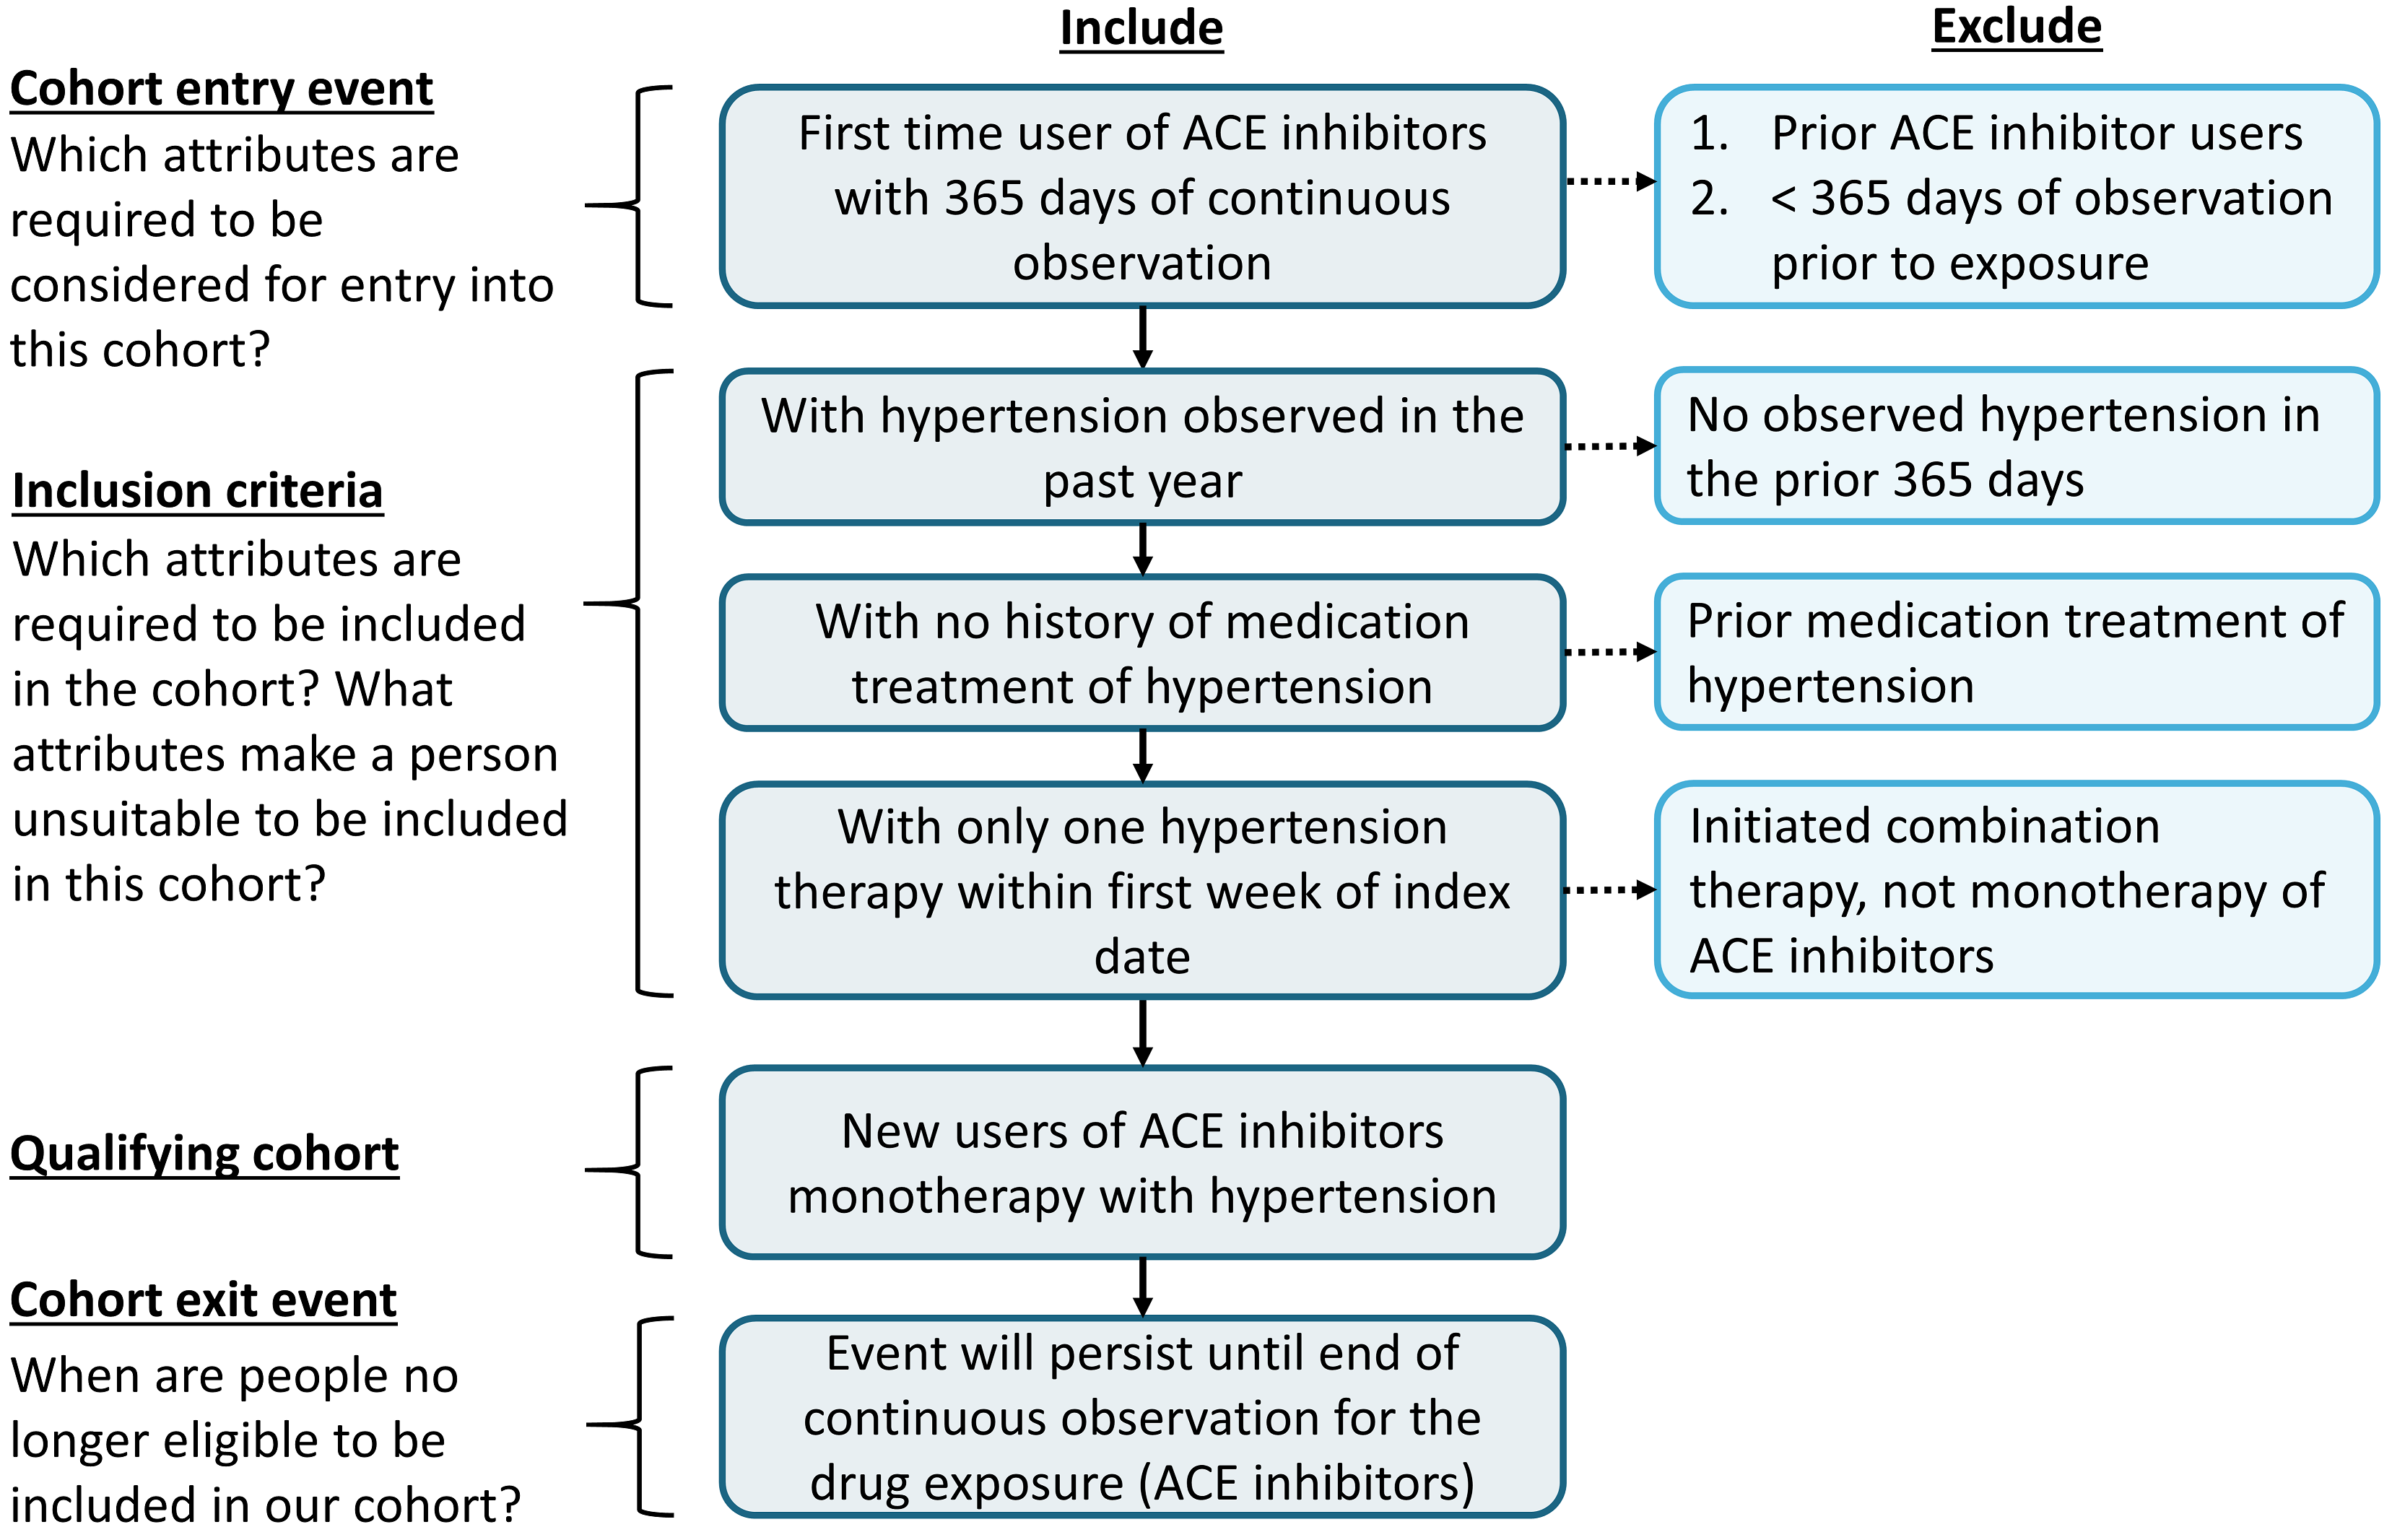
\includegraphics[width=1\linewidth]{images/Cohorts/CohortPractice} 

}

\caption{Diagramme Logique de la Cohorte Prévue}\label{fig:CohortPractice}
\end{figure}

Vous pouvez construire une cohorte dans l'interface utilisateur d'ATLAS ou vous pouvez écrire directement une requête contre votre CDM. Nous discuterons brièvement des deux dans ce chapitre.
\#\# Mise en œuvre d'une Cohorte avec ATLAS

Pour commencer avec ATLAS, cliquez sur le module 
\includegraphics{images/Cohorts/cohortdefinition.png}. Lorsque le module se charge, cliquez sur ``Nouvelle cohorte''. L'écran suivant que vous verrez sera une définition de cohorte vide. La Figure \ref{fig:ATLASdefineacohort} montre ce que vous verrez sur votre écran.

\begin{figure}

{\centering 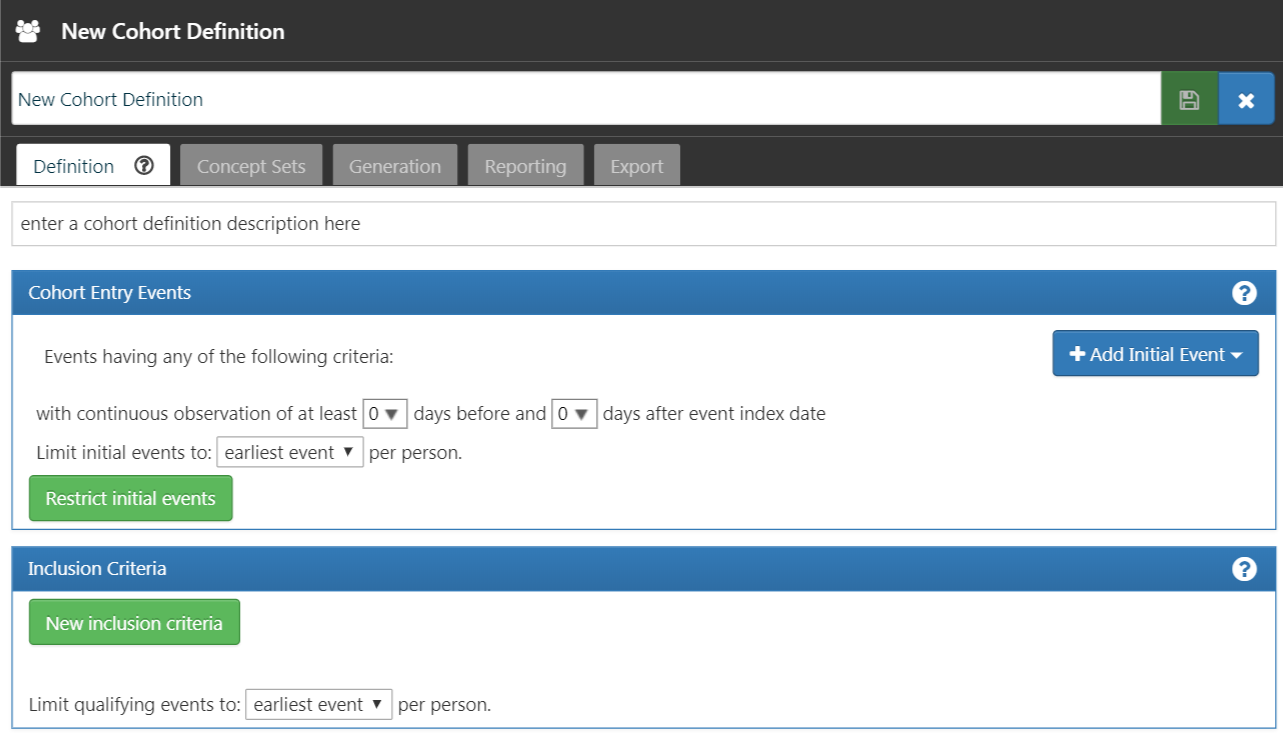
\includegraphics[width=1\linewidth]{images/Cohorts/ATLAS-defineacohort} 

}

\caption{Définition d'une Nouvelle Cohorte}\label{fig:ATLASdefineacohort}
\end{figure}

Avant de faire autre chose, il est recommandé de changer le nom de la cohorte de ``Nouvelle Définition de Cohorte'' à un nom unique pour cette cohorte. Vous pouvez opter pour un nom comme ``Nouveaux utilisateurs d'inhibiteurs de l'ECA en monothérapie de première ligne pour l'hypertension''.

\begin{rmdimportant}
ATLAS ne permet pas à deux cohortes d'avoir exactement les mêmes noms. ATLAS vous donnera un message d'erreur en pop-up si vous choisissez un nom déjà utilisé par une autre cohorte ATLAS.
\end{rmdimportant}

Une fois que vous avez choisi un nom, vous pouvez enregistrer la cohorte en cliquant sur 
\includegraphics{images/Cohorts/save.png}.

\subsection{Critères de l'Événement Initial}\label{crituxe8res-de-luxe9vuxe9nement-initial}

Maintenant nous pouvons procéder à la définition de l'événement initial de la cohorte. Cliquez sur ``Ajouter événement initial''. Vous devez maintenant choisir quel domaine vous construisez des critères autour. Vous pourriez vous demander, ``Comment savoir quel domaine est l'événement initial de la cohorte?'' Découvrons-le.

\begin{figure}

{\centering 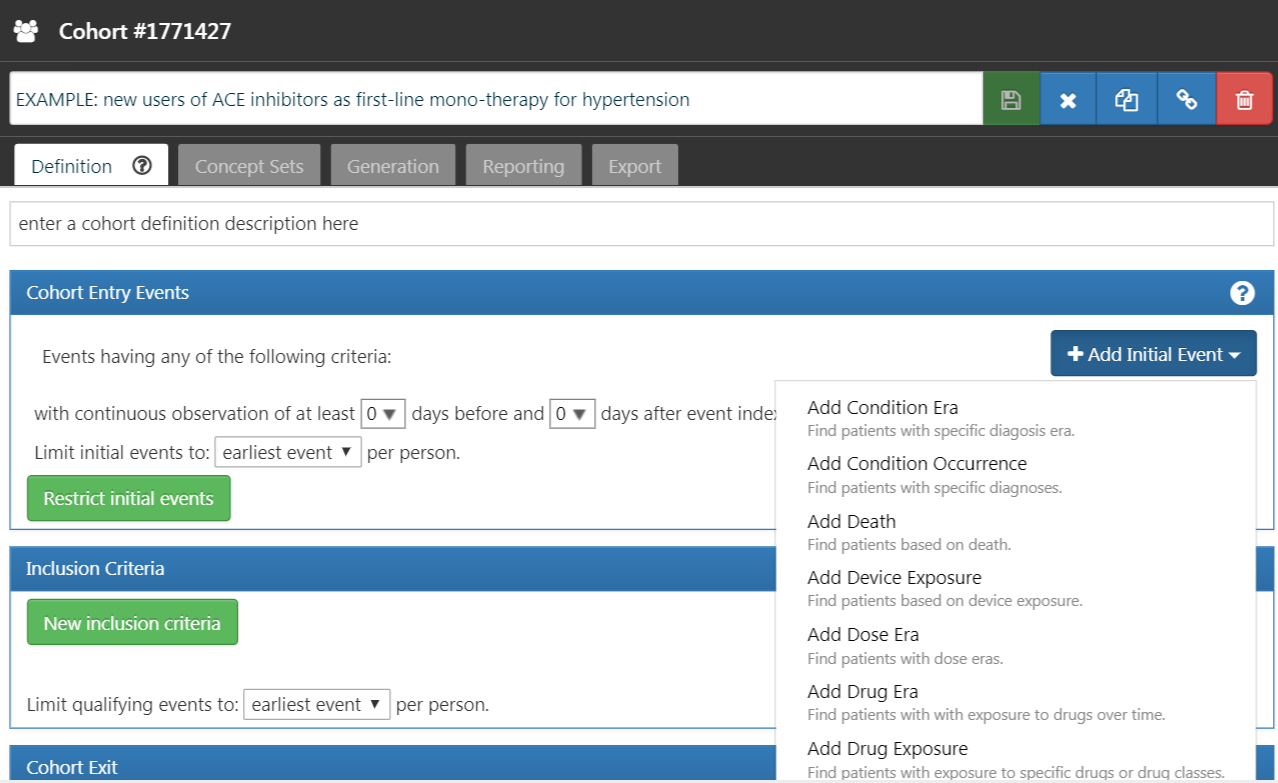
\includegraphics[width=1\linewidth]{images/Cohorts/ATLAS-initialevent} 

}

\caption{Ajout d'un Événement Initial}\label{fig:ATLASinitialevent}
\end{figure}

Comme nous le voyons dans la Figure \ref{fig:ATLASinitialevent}, ATLAS fournit des descriptions sous chaque critère pour vous aider. Si nous construisions des critères basés sur CONDITION\_OCCURRENCE, notre question porterait sur les patients avec un diagnostic spécifique. Si nous construisions des critères basés sur DRUG\_EXPOSURE, notre question porterait sur les patients prenant un médicament ou une classe de médicaments spécifiques. Puisque nous voulons trouver des patients qui commencent une monothérapie inhibiteurs de l'ECA en tant que traitements de première ligne pour l'hypertension, nous voulons choisir un critère DRUG\_EXPOSURE. Vous pourriez dire, ``Mais nous nous soucions également de l'hypertension en tant que diagnostic''. Vous avez raison. L'hypertension est un autre critère que nous allons construire. Cependant, la date de début de la cohorte est définie par le début du traitement par inhibiteur de l'ECA, qui est donc l'événement initial. Le diagnostic d'hypertension est ce que nous appelons un \emph{critère de qualification supplémentaire}. Nous y reviendrons une fois que nous aurons construit ce critère. Nous cliquerons sur ``Ajouter Exposition Médicamenteuse''.

L'écran se mettra à jour avec votre critère sélectionné mais vous n'avez pas encore terminé. Comme nous le voyons dans la Figure \ref{fig:ATLASdrugexposure}, ATLAS ne sait pas quel médicament nous recherchons. Nous devons dire à ATLAS quel ensemble de concepts est associé aux inhibiteurs de l'ECA.

\begin{figure}

{\centering 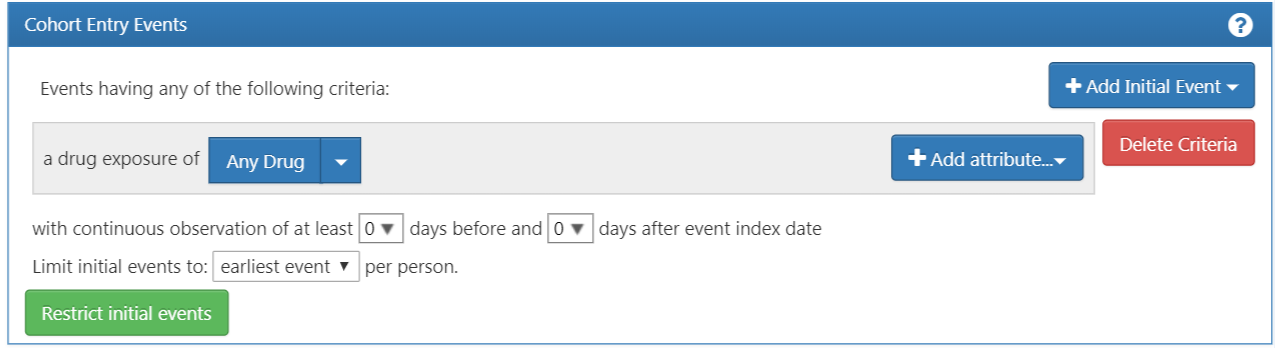
\includegraphics[width=1\linewidth]{images/Cohorts/ATLAS-drugexposure} 

}

\caption{Définition d'une Exposition Médicamenteuse}\label{fig:ATLASdrugexposure}
\end{figure}

\subsection{Définir l'Ensemble de Concepts}\label{duxe9finir-lensemble-de-concepts}

Vous devrez cliquer sur 
\includegraphics{images/Cohorts/downarrow.png} pour ouvrir la boîte de dialogue qui vous permettra de récupérer un ensemble de concepts pour définir les inhibiteurs de l'ECA.

\subsubsection*{Scénario 1 : Vous n'avez pas construit un Ensemble de Concepts}\label{scuxe9nario-1-vous-navez-pas-construit-un-ensemble-de-concepts}
\addcontentsline{toc}{subsubsection}{Scénario 1 : Vous n'avez pas construit un Ensemble de Concepts}

Si vous n'avez pas assemblé vos ensembles de concepts pour les appliquer à vos critères, vous devrez le faire avant de continuer. Vous pouvez construire un ensemble de concepts dans la définition de la cohorte en naviguant vers l'onglet ``Ensemble de concepts'' et en cliquant sur ``Nouvel Ensemble de Concepts''. Vous devrez renommer l'ensemble de concepts de ``Ensemble de Concepts non nommé'' à un nom de votre choix. De là, vous pouvez utiliser le module 
\includegraphics{images/Cohorts/search-2.png} pour rechercher des concepts cliniques représentant les inhibiteurs de l'ECA (Figure \ref{fig:aceinhibitors}).

\begin{figure}

{\centering 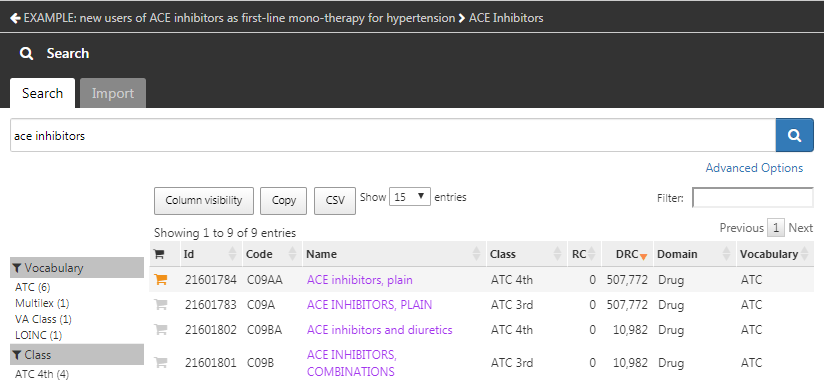
\includegraphics[width=1\linewidth]{images/Cohorts/aceinhibitors} 

}

\caption{Recherche dans le Vocabulaire - Inhibiteurs de l'ECA}\label{fig:aceinhibitors}
\end{figure}

Lorsque vous avez trouvé les termes que vous souhaitez utiliser pour définir cette exposition médicamenteuse, vous pouvez sélectionner le concept en cliquant sur \includegraphics{images/Cohorts/shoppingcart.png}. Vous pouvez retourner à votre définition de cohorte en utilisant la flèche gauche en haut à gauche de la Figure \ref{fig:aceinhibitors}. Vous pouvez vous référer au Chapitre \ref{StandardizedVocabularies} (Vocabulaires Standardisés) pour savoir comment naviguer les vocabulaires pour trouver les concepts cliniques d'intérêt.

La Figure \ref{fig:aceConceptSetExpression} montre notre expression de l'ensemble de concepts. Nous avons sélectionné tous les ingrédients inhibiteurs de l'ECA qui nous intéressent, et incluons tous leurs descendants, incluant ainsi tous les médicaments contenant l'un de ces ingrédients. Nous pouvons cliquer sur ``Concepts inclus'' pour voir tous les 21,536 concepts impliqués par cette expression, ou nous pouvons cliquer sur ``Codes Sources Inclus'' pour explorer tous les codes sources dans les différents systèmes de codage qui sont impliqués.

\begin{figure}

{\centering \includegraphics[width=1\linewidth]{images/Cohorts/aceConceptSetExpression} 

}

\caption{Un ensemble de concepts contenant des médicaments inhibiteurs de l'ECA.}\label{fig:aceConceptSetExpression}
\end{figure}

\subsubsection*{Scénario 2 : Vous avez déjà construit un Ensemble de Concepts}\label{scuxe9nario-2-vous-avez-duxe9juxe0-construit-un-ensemble-de-concepts}
\addcontentsline{toc}{subsubsection}{Scénario 2 : Vous avez déjà construit un Ensemble de Concepts}

Si vous avez déjà créé un ensemble de concepts et l'avez enregistré dans ATLAS, vous pouvez cliquer sur ``Importer un Ensemble de Concepts''. Une boîte de dialogue s'ouvrira et vous invitera à trouver votre concept dans le référentiel d'ensembles de concepts de votre ATLAS comme montré dans la Figure \ref{fig:ATLASfindyourconcept}. Dans la figure d'exemple, l'utilisateur récupère des ensembles de concepts stockés dans ATLAS. L'utilisateur a tapé le nom donné à cet ensemble de concepts ``inhibiteurs de l'ECA'' dans la recherche à droite. Cela a réduit la liste des ensembles de concepts uniquement aux concepts correspondants. De là, l'utilisateur peut cliquer sur la ligne de l'ensemble de concepts pour le sélectionner. (Note: La boîte de dialogue disparaîtra une fois que vous aurez sélectionné un ensemble de concepts.) Vous saurez que cette action a réussi lorsque la boîte Any Drug sera mise à jour avec le nom de l'ensemble de concepts que vous avez sélectionné.

\begin{figure}

{\centering \includegraphics[width=1\linewidth]{images/Cohorts/ATLAS-findingyourconcept} 

}

\caption{Importer un Ensemble de Concepts depuis le Référentiel ATLAS}\label{fig:ATLASfindyourconcept}
\end{figure}

\subsection{Critères Additionnels de l'Événement Initial}\label{crituxe8res-additionnels-de-luxe9vuxe9nement-initial}

Maintenant que vous avez attaché un ensemble de concepts, vous n'avez pas encore terminé. Votre question recherche de nouveaux utilisateurs ou la première fois dans l'historique de quelqu'un où ils sont exposés aux inhibiteurs de l'ECA. Cela se traduit par la \emph{première exposition} aux inhibiteurs de l'ECA dans le dossier du patient. Pour spécifier cela, vous devez cliquer sur ``+Ajouter attribut''. Vous voudrez sélectionner ``Ajouter le critère de première exposition''. Notez que vous pourriez spécifier d'autres attributs d'un critère que vous construisez. Vous pourriez spécifier un attribut de l'âge à l'occurrence, la date de l'occurrence, le genre ou d'autres attributs liés au médicament. Les critères disponibles à la sélection seront différents pour chaque domaine.

De là, la fenêtre se fermera automatiquement. Une fois sélectionné, cet attribut supplémentaire apparaîtra dans la même case que les critères initiaux (voir Figure \ref{fig:initialEventAce}).

\begin{rmdimportant}
La conception actuelle d'ATLAS peut en tromper certains. Malgré son apparence, le \includegraphics{images/Cohorts/redX.png} n'est pas destiné à signifier ``Non''. C'est une fonctionnalité actionnable qui permet à l'utilisateur de supprimer le critère. Si vous cliquez sur \includegraphics{images/Cohorts/redX.png}, ce critère disparaitra. Ainsi, vous devez laisser le critère avec le \includegraphics{images/Cohorts/redX.png} pour garder le critère actif.
\end{rmdimportant}

Maintenant que vous avez construit un événement de qualification initial. Pour vous assurer que vous capturez la première exposition médicamenteuse observée, vous voudrez ajouter une fenêtre de rétro-observation pour savoir que vous regardez suffisamment de l'historique du patient pour savoir ce qui vient en premier. Il est possible qu'un patient avec une période d'observation courte ait reçu une exposition ailleurs que nous ne voyons pas. Nous ne pouvons pas contrôler cela mais nous pouvons mandater une durée minimale de temps pendant laquelle le patient doit être dans les données avant la date d'index. Vous pouvez le faire en ajustant les listes déroulantes d'observation continue. Vous pouvez également cliquer sur la boîte et taper une valeur pour ces fenêtres. Nous exigerons 365 jours d'observation continue avant l'événement initial. Vous mettrez à jour votre période d'observation à : \emph{avec observation continue de 365 jours avant}, comme montré dans la Figure \ref{fig:initialEventAce}. Cette fenêtre de rétro-observation est à la discrétion de votre équipe d'étude. Vous pouvez choisir différemment pour d'autres cohortes. Cela crée, autant que nous le pouvons, une période minimale de temps où nous voyons le patient pour s'assurer que nous capturons le premier enregistrement. Ce critère concerne l'historique préalable et n'implique pas de temps après l'événement d'index. Par conséquent, nous exigeons 0 jours après l'événement d'index. Notre événement de qualification est l'utilisation pour la première fois des inhibiteurs de l'ECA. Ainsi, nous limitons les événements initiaux au ``premier événement'' par personne.

\begin{figure}

{\centering \includegraphics[width=1\linewidth]{images/Cohorts/initialEventAce} 

}

\caption{Définir l'observation continue requise avant la date d'index.}\label{fig:initialEventAce}
\end{figure}

Pour mieux expliquer comment cette logique se met en place, vous pouvez penser assembler des chronologies de patients.

\begin{figure}

{\centering \includegraphics[width=1\linewidth]{images/Cohorts/EarliestEventExplained} 

}

\caption{Explication de l'éligibilité des patients par critères appliqués}\label{fig:EarliestEventExplained}
\end{figure}

Dans la Figure \ref{fig:EarliestEventExplained}, chaque ligne représente un patient unique qui peut être éligible pour rejoindre la cohorte. Les étoiles remplies représentent un moment où le patient remplit les critères spécifiés. Au fur et à mesure que des critères supplémentaires sont appliqués, vous pouvez voir que certaines étoiles sont d'une teinte plus claire. Cela signifie que ces patients ont d'autres enregistrements remplissant les critères mais il y a un autre enregistrement qui précède cela. Au moment où nous arrivons au dernier critère, nous examinons la vue cumulative des patients qui ont des inhibiteurs de l'ECA pour la première fois et ont 365 jours avant la première fois de l'occurrence. Logiquement, limiter à l'événement initial est redondant bien que cela soit utile de maintenir notre logique explicite dans chaque sélection que nous faisons. Lorsque vous construisez vos propres cohortes, vous pouvez choisir de consulter la section Chercheurs du \href{http://forums.ohdsi.org}{Forum OHDSI} pour obtenir un second avis sur la façon de construire votre logique de cohorte.

\subsection{Critères d'Inclusion}\label{crituxe8res-dinclusion}

Une fois que nous avons spécifié un événement d'entrée de cohorte, vous pouvez procéder à l'un des deux endroits pour ajouter vos événements de qualification supplémentaires : ``Restreindre les événements initiaux'' et ``Nouveaux critères d'inclusion''. La différence fondamentale entre ces deux options est l'information intérimaire que vous voulez qu'ATLAS vous renvoie. Si vous ajoutez des critères de qualification supplémentaires dans la boîte d'événement d'entrée de la cohorte en sélectionnant ``Restreindre les événements initiaux'', lorsque vous choisissez de générer un compte dans ATLAS, vous recevrez uniquement le nombre de personnes qui remplissent TOUS ces critères. Si vous choisissez d'ajouter des critères dans ``Nouveaux critères d'inclusion'', vous obtiendrez un graphique d'attrition pour vous montrer combien de patients sont perdus en appliquant des critères d'inclusion supplémentaires. Il est fortement encouragé d'utiliser la section des Critères d'Inclusion afin de comprendre l'impact de chaque règle sur le succès global de la définition de la cohorte. Vous pouvez trouver un certain critère d'inclusion limitant sévèrement le nombre de personnes qui finissent dans la cohorte. Vous pouvez choisir de relâcher ce critère pour obtenir une cohorte plus large. Cela sera finalement à la discrétion du consensus expert assemblant cette cohorte.

Vous voudrez maintenant cliquer sur ``Nouveaux critères d'inclusion'' pour ajouter une logique supplémentaire sur l'appartenance à cette cohorte. La fonctionnalité de cette section est identique à la façon dont nous avons discuté de la construction des critères de cohorte ci-dessus. Vous pouvez spécifier les critères et ajouter des attributs spécifiques. Notre premier critère supplémentaire est de sous-ensemble la cohorte seulement aux patients: \emph{Avec au moins 1 occurrence d'un trouble hypertensif entre 365 et 0 jours après la date d'index (premières initiations d'un inhibiteur de l'ECA)}. Vous cliquerez sur ``Nouveaux critères d'inclusion'' pour ajouter un nouveau critère. Vous devez nommer votre critère et, si vous le souhaitez, mettre une petite description de ce que vous recherchez. Cela est pour vos propres besoins pour se rappeler ce que vous construisez -- cela n'impactera pas l'intégrité de la cohorte que vous définissez.

Une fois que vous avez annoté ce nouveau critère, vous cliquerez sur le bouton ``+Ajouter un critère au groupe'' pour construire votre critère réel pour cette règle. Ce bouton fonctionne de manière similaire au bouton ``Ajouter événement initial'' sauf que nous ne spécifions plus d'événement initial. Nous pourrions ajouter plusieurs critères à cela -- c'est pourquoi il spécifie ``ajouter un critère au groupe''. Un exemple serait si vous avez plusieurs façons de trouver une maladie (par exemple, une logique pour un CONDITION\_OCCURRENCE, une logique utilisant un DRUG\_EXPOSURE comme proxy pour cette condition, une logique utilisant une MEASUREMENT comme proxy pour cette condition). Ceux-ci seraient des domaines séparés et nécessiteraient des critères différents mais peuvent être regroupés en un critère recherchant cette condition. Dans ce cas, nous voulons trouver un diagnostic de l'hypertension donc nous ``Ajoutons une occurrence de condition''. Nous suivrons des étapes similaires à celles de l'événement initial en attachant un ensemble de concepts à cet enregistrement. Nous voulons également spécifier que l'événement commence entre 365 jours avant et 0 jours après la date d'index (l'occurrence de la première utilisation d'un inhibiteur de l'ECA). Vérifiez maintenant votre logique par rapport à la Figure \ref{fig:ATLASIC1}.

\begin{figure}

{\centering \includegraphics[width=1\linewidth]{images/Cohorts/ATLAS-IC1} 

}

\caption{Critères d'Inclusion Supplémentaires 1}\label{fig:ATLASIC1}
\end{figure}

Vous voudrez ensuite ajouter un autre critère pour rechercher des patients: \emph{avec exactement 0 occurrences de médicaments contre l'hypertension TOUS les jours avant et 1 jour avant la date d'index (aucune exposition à des médicaments anti-hypertensifs avant un inhibiteur de l'ECA)}. Ce processus commence comme avant en cliquant sur le bouton ``Nouveaux critères d'inclusion'', en ajoutant vos annotations à ce critère, puis en cliquant sur ``+Ajouter un critère au groupe''. Il s'agit d'une DRUG\_EXPOSURE, donc vous cliquerez sur ``Ajouter Exposition Médicamenteuse'', attacherez un ensemble de concepts pour les médicaments anti-hypertensifs, et spécifierez TOUS les jours avant et 0 jours après (ou ``1 jours avant'' est équivalent comme vu dans la figure) la date d'index. Assurez-vous de confirmer que vous avez sélectionné \emph{exactement 0} occurrence. Vérifiez maintenant votre logique par rapport à la Figure \ref{fig:ATLASIC2}.

\begin{figure}

{\centering \includegraphics[width=1\linewidth]{images/Cohorts/ATLAS-IC2} 

}

\caption{Critères d'Inclusion Supplémentaires 2}\label{fig:ATLASIC2}
\end{figure}

Vous pourriez être confus pourquoi ``ne pas avoir d'occurrences'' est codé comme ``exactement 0 occurrences''. C'est une nuance de la façon dont ATLAS consomme la connaissance. ATLAS consomme uniquement les critères d'inclusion. Vous devez utiliser des opérateurs logiques pour indiquer quand vous voulez l'absence d'un attribut spécifique comme: ``Exactement 0''. Au fil du temps, vous vous familiariserez avec les opérateurs logiques disponibles dans les critères ATLAS.

Enfin, vous voudrez ajouter un autre critère pour rechercher des patients: \emph{avec exactement 1 occurrence de médicaments contre l'hypertension entre 0 jours avant et 7 jours après la date d'index ET ne peut commencer qu'un seul médicament HT (un inhibiteur de l'ECA)}. Ce processus commence comme avant en cliquant sur le bouton ``Nouveaux critères d'inclusion'', en ajoutant vos annotations à ce critère, puis en cliquant sur ``+Ajouter un critère au groupe''. Il s'agit d'un DRUG\_ERA donc vous cliquerez sur ``Ajouter Époque Médicamenteuse'', attacherez un ensemble de concepts pour les médicaments anti-hypertensifs, et spécifierez 0 jours avant et 7 jours après la date d'index. Vérifiez maintenant votre logique
\#\# Implémentation de la Cohorte en Utilisant SQL

Ici, nous décrivons comment créer la même cohorte, mais en utilisant SQL et R. Comme discuté dans le Chapitre \ref{SqlAndR}, OHDSI fournit deux packages R, appelés SqlRender et DatabaseConnector, qui permettent ensemble d'écrire du code SQL pouvant être automatiquement traduit et exécuté sur une grande variété de plateformes de bases de données.

Pour plus de clarté, nous allons diviser le SQL en plusieurs morceaux, chaque morceau générant une table temporaire utilisée dans le suivant. Ce n'est probablement pas la méthode la plus efficace d'un point de vue computationnel, mais elle est plus facile à lire qu'une seule déclaration très longue.

\subsection{Connexion à la Base de Données}\label{connexion-uxe0-la-base-de-donnuxe9es}

Nous devons d'abord indiquer à R comment se connecter au serveur. Nous utilisons le package \href{https://ohdsi.github.io/DatabaseConnector/}{DatabaseConnector}, qui fournit une fonction appelée \texttt{createConnectionDetails}. Tapez \texttt{?createConnectionDetails} pour les paramètres spécifiques requis pour les divers systèmes de gestion de base de données (SGDB). Par exemple, on pourrait se connecter à une base de données PostgreSQL en utilisant ce code :

\begin{Shaded}
\begin{Highlighting}[]
\FunctionTok{library}\NormalTok{(CohortMethod)}
\NormalTok{connDetails }\OtherTok{\textless{}{-}} \FunctionTok{createConnectionDetails}\NormalTok{(}\AttributeTok{dbms =} \StringTok{"postgresql"}\NormalTok{,}
                                       \AttributeTok{server =} \StringTok{"localhost/ohdsi"}\NormalTok{,}
                                       \AttributeTok{user =} \StringTok{"joe"}\NormalTok{,}
                                       \AttributeTok{password =} \StringTok{"supersecret"}\NormalTok{)}

\NormalTok{cdmDbSchema }\OtherTok{\textless{}{-}} \StringTok{"my\_cdm\_data"}
\NormalTok{cohortDbSchema }\OtherTok{\textless{}{-}} \StringTok{"scratch"}
\NormalTok{cohortTable }\OtherTok{\textless{}{-}} \StringTok{"my\_cohorts"}
\end{Highlighting}
\end{Shaded}

Les trois dernières lignes définissent les variables \texttt{cdmDbSchema}, \texttt{cohortDbSchema} et \texttt{cohortTable}. Nous les utiliserons plus tard pour indiquer à R où les données au format CDM se trouvent, et où les cohortes d'intérêt doivent être créées. Notez que pour Microsoft SQL Server, les schémas de base de données doivent spécifier à la fois la base de données et le schéma, par exemple \texttt{cdmDbSchema\ \textless{}-\ "my\_cdm\_data.dbo"}.

\subsection{Spécification des Concepts}\label{spuxe9cification-des-concepts}

Pour plus de lisibilité, nous allons définir les IDs de concepts nécessaires dans R et les passer au SQL :

\begin{Shaded}
\begin{Highlighting}[]
\NormalTok{aceI }\OtherTok{\textless{}{-}} \FunctionTok{c}\NormalTok{(}\DecValTok{1308216}\NormalTok{, }\DecValTok{1310756}\NormalTok{, }\DecValTok{1331235}\NormalTok{, }\DecValTok{1334456}\NormalTok{, }\DecValTok{1335471}\NormalTok{, }\DecValTok{1340128}\NormalTok{, }\DecValTok{1341927}\NormalTok{,}
          \DecValTok{1342439}\NormalTok{, }\DecValTok{1363749}\NormalTok{, }\DecValTok{1373225}\NormalTok{)}

\NormalTok{hypertension }\OtherTok{\textless{}{-}} \DecValTok{316866}

\NormalTok{allHtDrugs }\OtherTok{\textless{}{-}} \FunctionTok{c}\NormalTok{(}\DecValTok{904542}\NormalTok{, }\DecValTok{907013}\NormalTok{, }\DecValTok{932745}\NormalTok{, }\DecValTok{942350}\NormalTok{, }\DecValTok{956874}\NormalTok{, }\DecValTok{970250}\NormalTok{, }\DecValTok{974166}\NormalTok{,}
                  \DecValTok{978555}\NormalTok{, }\DecValTok{991382}\NormalTok{, }\DecValTok{1305447}\NormalTok{, }\DecValTok{1307046}\NormalTok{, }\DecValTok{1307863}\NormalTok{, }\DecValTok{1308216}\NormalTok{,}
                  \DecValTok{1308842}\NormalTok{, }\DecValTok{1309068}\NormalTok{, }\DecValTok{1309799}\NormalTok{, }\DecValTok{1310756}\NormalTok{, }\DecValTok{1313200}\NormalTok{, }\DecValTok{1314002}\NormalTok{,}
                  \DecValTok{1314577}\NormalTok{, }\DecValTok{1317640}\NormalTok{, }\DecValTok{1317967}\NormalTok{, }\DecValTok{1318137}\NormalTok{, }\DecValTok{1318853}\NormalTok{, }\DecValTok{1319880}\NormalTok{,}
                  \DecValTok{1319998}\NormalTok{, }\DecValTok{1322081}\NormalTok{, }\DecValTok{1326012}\NormalTok{, }\DecValTok{1327978}\NormalTok{, }\DecValTok{1328165}\NormalTok{, }\DecValTok{1331235}\NormalTok{,}
                  \DecValTok{1332418}\NormalTok{, }\DecValTok{1334456}\NormalTok{, }\DecValTok{1335471}\NormalTok{, }\DecValTok{1338005}\NormalTok{, }\DecValTok{1340128}\NormalTok{, }\DecValTok{1341238}\NormalTok{,}
                  \DecValTok{1341927}\NormalTok{, }\DecValTok{1342439}\NormalTok{, }\DecValTok{1344965}\NormalTok{, }\DecValTok{1345858}\NormalTok{, }\DecValTok{1346686}\NormalTok{, }\DecValTok{1346823}\NormalTok{,}
                  \DecValTok{1347384}\NormalTok{, }\DecValTok{1350489}\NormalTok{, }\DecValTok{1351557}\NormalTok{, }\DecValTok{1353766}\NormalTok{, }\DecValTok{1353776}\NormalTok{, }\DecValTok{1363053}\NormalTok{,}
                  \DecValTok{1363749}\NormalTok{, }\DecValTok{1367500}\NormalTok{, }\DecValTok{1373225}\NormalTok{, }\DecValTok{1373928}\NormalTok{, }\DecValTok{1386957}\NormalTok{, }\DecValTok{1395058}\NormalTok{,}
                  \DecValTok{1398937}\NormalTok{, }\DecValTok{40226742}\NormalTok{, }\DecValTok{40235485}\NormalTok{)}
\end{Highlighting}
\end{Shaded}

\subsection{Trouver la Première Utilisation}\label{trouver-la-premiuxe8re-utilisation}

Nous allons d'abord trouver la première utilisation des inhibiteurs de l'ECA pour chaque patient :

\begin{Shaded}
\begin{Highlighting}[]
\NormalTok{conn }\OtherTok{\textless{}{-}} \FunctionTok{connect}\NormalTok{(connectionDetails)}

\NormalTok{sql }\OtherTok{\textless{}{-}} \StringTok{"SELECT person\_id AS subject\_id,}
\StringTok{  MIN(drug\_exposure\_start\_date) AS cohort\_start\_date}
\StringTok{INTO \#first\_use}
\StringTok{FROM @cdm\_db\_schema.drug\_exposure}
\StringTok{INNER JOIN @cdm\_db\_schema.concept\_ancestor}
\StringTok{  ON descendant\_concept\_id = drug\_concept\_id}
\StringTok{WHERE ancestor\_concept\_id IN (@ace\_i)}
\StringTok{GROUP BY person\_id;"}

\FunctionTok{renderTranslateExecuteSql}\NormalTok{(conn,}
\NormalTok{                          sql,}
                          \AttributeTok{cdm\_db\_schema =}\NormalTok{ cdmDbSchema,}
                          \AttributeTok{ace\_i =}\NormalTok{ aceI)}
\end{Highlighting}
\end{Shaded}

Notez que nous rejoignons la table DRUG\_EXPOSURE à la table CONCEPT\_ANCESTOR pour trouver tous les médicaments contenant un inhibiteur de l'ECA.

\subsection{Exiger 365 Jours d'Observation Préalable}\label{exiger-365-jours-dobservation-pruxe9alable}

Ensuite, nous exigeons 365 jours d'observation continue préalable en rejoignant la table OBSERVATION\_PERIOD :

\begin{Shaded}
\begin{Highlighting}[]
\NormalTok{sql }\OtherTok{\textless{}{-}} \StringTok{"SELECT subject\_id,}
\StringTok{  cohort\_start\_date}
\StringTok{INTO \#has\_prior\_obs}
\StringTok{FROM \#first\_use}
\StringTok{INNER JOIN @cdm\_db\_schema.observation\_period}
\StringTok{  ON subject\_id = person\_id}
\StringTok{    AND observation\_period\_start\_date \textless{}= cohort\_start\_date}
\StringTok{    AND observation\_period\_end\_date \textgreater{}= cohort\_start\_date}
\StringTok{WHERE DATEADD(DAY, 365, observation\_period\_start\_date) \textless{} cohort\_start\_date;"}

\FunctionTok{renderTranslateExecuteSql}\NormalTok{(conn, sql, }\AttributeTok{cdm\_db\_schema =}\NormalTok{ cdmDbSchema)}
\end{Highlighting}
\end{Shaded}

\subsection{Exiger une Hypertension Préalable}\label{exiger-une-hypertension-pruxe9alable}

Nous exigeons un diagnostic d'hypertension dans les 365 jours précédents :

\begin{Shaded}
\begin{Highlighting}[]
\NormalTok{sql }\OtherTok{\textless{}{-}} \StringTok{"SELECT DISTINCT subject\_id,}
\StringTok{  cohort\_start\_date}
\StringTok{INTO \#has\_ht}
\StringTok{FROM \#has\_prior\_obs}
\StringTok{INNER JOIN @cdm\_db\_schema.condition\_occurrence}
\StringTok{  ON subject\_id = person\_id}
\StringTok{    AND condition\_start\_date \textless{}= cohort\_start\_date}
\StringTok{    AND condition\_start\_date \textgreater{}= DATEADD(DAY, {-}365, cohort\_start\_date)}
\StringTok{INNER JOIN @cdm\_db\_schema.concept\_ancestor}
\StringTok{  ON descendant\_concept\_id = condition\_concept\_id}
\StringTok{WHERE ancestor\_concept\_id = @hypertension;"}

\FunctionTok{renderTranslateExecuteSql}\NormalTok{(conn,}
\NormalTok{                          sql,}
                          \AttributeTok{cdm\_db\_schema =}\NormalTok{ cdmDbSchema,}
                          \AttributeTok{hypertension =}\NormalTok{ hypertension)}
\end{Highlighting}
\end{Shaded}

Notez que nous \texttt{SELECT\ DISTINCT}, car sinon si une personne a plusieurs diagnostics d'hypertension dans son passé, nous créerions des entrées de cohorte en double.

\subsection{Pas de Traitement Préalable}\label{pas-de-traitement-pruxe9alable}

Nous exigeons aucune exposition préalable à un traitement de l'hypertension :

\begin{Shaded}
\begin{Highlighting}[]
\NormalTok{sql }\OtherTok{\textless{}{-}} \StringTok{"SELECT subject\_id,}
\StringTok{  cohort\_start\_date}
\StringTok{INTO \#no\_prior\_ht\_drugs}
\StringTok{FROM \#has\_ht}
\StringTok{LEFT JOIN (}
\StringTok{  SELECT *}
\StringTok{  FROM @cdm\_db\_schema.drug\_exposure}
\StringTok{  INNER JOIN @cdm\_db\_schema.concept\_ancestor}
\StringTok{    ON descendant\_concept\_id = drug\_concept\_id}
\StringTok{  WHERE ancestor\_concept\_id IN (@all\_ht\_drugs)}
\StringTok{) ht\_drugs}
\StringTok{  ON subject\_id = person\_id}
\StringTok{    AND drug\_exposure\_start\_date \textless{} cohort\_start\_date}
\StringTok{WHERE person\_id IS NULL;"}

\FunctionTok{renderTranslateExecuteSql}\NormalTok{(conn,}
\NormalTok{                          sql,}
                          \AttributeTok{cdm\_db\_schema =}\NormalTok{ cdmDbSchema,}
                          \AttributeTok{all\_ht\_drugs =}\NormalTok{ allHtDrugs)}
\end{Highlighting}
\end{Shaded}

Notez que nous utilisons une jonction gauche, et nous n'autorisons que les lignes où le person\_id, qui vient de la table DRUG\_EXPOSURE, est NULL, ce qui signifie qu'aucun enregistrement correspondant n'a été trouvé.

\subsection{Monothérapie}\label{monothuxe9rapie}

Nous exigeons qu'il n'y ait qu'une seule exposition au traitement de l'hypertension dans les sept premiers jours suivant l'entrée dans la cohorte :

\begin{Shaded}
\begin{Highlighting}[]
\NormalTok{sql }\OtherTok{\textless{}{-}} \StringTok{"SELECT subject\_id,}
\StringTok{  cohort\_start\_date}
\StringTok{INTO \#monotherapy}
\StringTok{FROM \#no\_prior\_ht\_drugs}
\StringTok{INNER JOIN @cdm\_db\_schema.drug\_exposure}
\StringTok{  ON subject\_id = person\_id}
\StringTok{    AND drug\_exposure\_start\_date \textgreater{}= cohort\_start\_date}
\StringTok{    AND drug\_exposure\_start\_date \textless{}= DATEADD(DAY, 7, cohort\_start\_date)}
\StringTok{INNER JOIN @cdm\_db\_schema.concept\_ancestor}
\StringTok{  ON descendant\_concept\_id = drug\_concept\_id}
\StringTok{WHERE ancestor\_concept\_id IN (@all\_ht\_drugs)}
\StringTok{GROUP BY subject\_id,}
\StringTok{  cohort\_start\_date}
\StringTok{HAVING COUNT(*) = 1;"}

\FunctionTok{renderTranslateExecuteSql}\NormalTok{(conn,}
\NormalTok{                          sql,}
                          \AttributeTok{cdm\_db\_schema =}\NormalTok{ cdmDbSchema,}
                          \AttributeTok{all\_ht\_drugs =}\NormalTok{ allHtDrugs)}
\end{Highlighting}
\end{Shaded}

\subsection{Sortie de la Cohorte}\label{sortie-de-la-cohorte}

Nous avons maintenant spécifié complètement notre cohorte sauf la date de fin de la cohorte. La cohorte est définie pour se terminer lorsque l'exposition s'arrête, permettant un écart maximum de 30 jours entre les expositions subséquentes. Cela signifie que nous devons non seulement considérer la première exposition au médicament, mais aussi les expositions suivantes aux inhibiteurs de l'ECA. Le SQL pour combiner les expositions subséquentes en ères peut être très complexe. Heureusement, du code standard a été défini pour créer efficacement des ères. (Ce code a été écrit par Chris Knoll, et est souvent appelé au sein de l'OHDSI comme `la magie'). Nous créons d'abord une table temporaire contenant toutes les expositions que nous souhaitons fusionner :

\begin{Shaded}
\begin{Highlighting}[]
\NormalTok{sql }\OtherTok{\textless{}{-}} \StringTok{"}
\StringTok{  SELECT person\_id,}
\StringTok{    CAST(1 AS INT) AS concept\_id,}
\StringTok{    drug\_exposure\_start\_date AS exposure\_start\_date,}
\StringTok{    drug\_exposure\_end\_date AS exposure\_end\_date}
\StringTok{  INTO \#exposure}
\StringTok{  FROM @cdm\_db\_schema.drug\_exposure}
\StringTok{  INNER JOIN @cdm\_db\_schema.concept\_ancestor}
\StringTok{    ON descendant\_concept\_id = drug\_concept\_id}
\StringTok{  WHERE ancestor\_concept\_id IN (@ace\_i);"}
\FunctionTok{renderTranslateExecuteSql}\NormalTok{(conn,}
\NormalTok{                          sql,}
                          \AttributeTok{cdm\_db\_schema =}\NormalTok{ cdmDbSchema,}
                          \AttributeTok{ace\_i =}\NormalTok{ aceI)}
\end{Highlighting}
\end{Shaded}

Nous exécutons ensuite le code standard pour fusionner les expositions séquentielles :

\begin{Shaded}
\begin{Highlighting}[]
\NormalTok{sql }\OtherTok{\textless{}{-}} \StringTok{"}
\StringTok{SELECT ends.person\_id AS subject\_id,}
\StringTok{    ends.concept\_id AS cohort\_definition\_id,}
\StringTok{  MIN(exposure\_start\_date) AS cohort\_start\_date,}
\StringTok{  ends.era\_end\_date AS cohort\_end\_date}
\StringTok{INTO \#exposure\_era}
\StringTok{FROM (}
\StringTok{  SELECT exposure.person\_id,}
\StringTok{    exposure.concept\_id,}
\StringTok{    exposure.exposure\_start\_date,}
\StringTok{    MIN(events.end\_date) AS era\_end\_date}
\StringTok{  FROM \#exposure exposure}
\StringTok{  JOIN (}
\StringTok{{-}{-}cteEndDates}
\StringTok{    SELECT person\_id,}
\StringTok{      concept\_id,}
\StringTok{      DATEADD(DAY, {-} 1 * @max\_gap, event\_date) AS end\_date}
\StringTok{    FROM (}
\StringTok{      SELECT person\_id,}
\StringTok{        concept\_id,}
\StringTok{        event\_date,}
\StringTok{        event\_type,}
\StringTok{        MAX(start\_ordinal) OVER (}
\StringTok{          PARTITION BY person\_id ,concept\_id ORDER BY event\_date,}
\StringTok{              event\_type ROWS UNBOUNDED PRECEDING}
\StringTok{          ) AS start\_ordinal,}
\StringTok{        ROW\_NUMBER() OVER (}
\StringTok{          PARTITION BY person\_id, concept\_id ORDER BY event\_date,}
\StringTok{            event\_type}
\StringTok{          ) AS overall\_ord}
\StringTok{      FROM (}
\StringTok{{-}{-} select the start dates, assigning a row number to each}
\StringTok{        SELECT person\_id,}
\StringTok{          concept\_id,}
\StringTok{          exposure\_start\_date AS event\_date,}
\StringTok{          0 AS event\_type,}
\StringTok{          ROW\_NUMBER() OVER (}
\StringTok{            PARTITION BY person\_id, concept\_id ORDER BY exposure\_start\_date}
\StringTok{            ) AS start\_ordinal}
\StringTok{        FROM \#exposure exposure}

\StringTok{        UNION ALL}
\StringTok{{-}{-} add the end dates with NULL as the row number, padding the end dates by}
\StringTok{{-}{-} @max\_gap to allow a grace period for overlapping ranges.}

\StringTok{        SELECT person\_id,}
\StringTok{          concept\_id,}
\StringTok{          DATEADD(day, @max\_gap, exposure\_end\_date),}
\StringTok{          1 AS event\_type,}
\StringTok{          NULL}
\StringTok{        FROM \#exposure exposure}
\StringTok{        ) rawdata}
\StringTok{    ) events}
\StringTok{  WHERE 2 * events.start\_ordinal {-} events.overall\_ord = 0}
\StringTok{  ) events}
\StringTok{  ON exposure.person\_id = events.person\_id}
\StringTok{      AND exposure.concept\_id = events.concept\_id}
\StringTok{      AND events.end\_date \textgreater{}= exposure.exposure\_end\_date}
\StringTok{  GROUP BY exposure.person\_id,}
\StringTok{      exposure.concept\_id,}
\StringTok{      exposure.exposure\_start\_date}
\StringTok{  ) ends}
\StringTok{GROUP BY ends.person\_id,}
\StringTok{  concept\_id,}
\StringTok{  ends.era\_end\_date;"}

\FunctionTok{renderTranslateExecuteSql}\NormalTok{(conn,}
\NormalTok{                          sql,}
                          \AttributeTok{cdm\_db\_schema =}\NormalTok{ cdmDbSchema,}
                          \AttributeTok{max\_gap =} \DecValTok{30}\NormalTok{)}
\end{Highlighting}
\end{Shaded}

Ce code fusionne toutes les expositions subséquentes, permettant un écart entre les expositions tel que défini par l'argument \texttt{max\_gap}. Les ères d'exposition aux médicaments résultants sont écrites dans une table temporaire appelée \texttt{\#exposure\_era}.

Ensuite, nous joignons simplement ces ères d'exposition aux inhibiteurs de l'ECA à notre cohorte d'origine pour utiliser les dates de fin des ères comme nos dates de fin de cohorte :

\begin{Shaded}
\begin{Highlighting}[]
\NormalTok{sql }\OtherTok{\textless{}{-}} \StringTok{"SELECT ee.subject\_id,}
\StringTok{  CAST(1 AS INT) AS cohort\_definition\_id,}
\StringTok{  ee.cohort\_start\_date,}
\StringTok{  ee.cohort\_end\_date}
\StringTok{INTO @cohort\_db\_schema.@cohort\_table}
\StringTok{FROM \#monotherapy mt}
\StringTok{INNER JOIN \#exposure\_era ee}
\StringTok{  ON mt.subject\_id = ee.subject\_id}
\StringTok{    AND mt.cohort\_start\_date = ee.cohort\_start\_date;"}

\FunctionTok{renderTranslateExecuteSql}\NormalTok{(conn,}
\NormalTok{                          sql,}
                          \AttributeTok{cohort\_db\_schema =}\NormalTok{ cohortDbSchema,}
                          \AttributeTok{cohort\_table =}\NormalTok{ cohortTable)}
\end{Highlighting}
\end{Shaded}

Ici, nous stockons la cohorte finale dans le schéma et la table que nous avons définis précédemment. Nous lui attribuons un ID de définition de cohorte de 1, pour la distinguer d'autres cohortes que nous pourrions vouloir stocker dans la même table.

\subsection{Nettoyage}\label{nettoyage-1}

Enfin, il est toujours recommandé de nettoyer toutes les tables temporaires qui ont été créées et de se déconnecter du serveur de la base de données :

\begin{Shaded}
\begin{Highlighting}[]
\NormalTok{sql }\OtherTok{\textless{}{-}} \StringTok{"TRUNCATE TABLE \#first\_use;}
\StringTok{DROP TABLE \#first\_use;}

\StringTok{TRUNCATE TABLE \#has\_prior\_obs;}
\StringTok{DROP TABLE \#has\_prior\_obs;}

\StringTok{TRUNCATE TABLE \#has\_ht;}
\StringTok{DROP TABLE \#has\_ht;}

\StringTok{TRUNCATE TABLE \#no\_prior\_ht\_drugs;}
\StringTok{DROP TABLE \#no\_prior\_ht\_drugs;}

\StringTok{TRUNCATE TABLE \#monotherapy;}
\StringTok{DROP TABLE \#monotherapy;}

\StringTok{TRUNCATE TABLE \#exposure;}
\StringTok{DROP TABLE \#exposure;}

\StringTok{TRUNCATE TABLE \#exposure\_era;}
\StringTok{DROP TABLE \#exposure\_era;"}

\FunctionTok{renderTranslateExecuteSql}\NormalTok{(conn, sql)}

\FunctionTok{disconnect}\NormalTok{(conn)}
\end{Highlighting}
\end{Shaded}

\section{Résumé}\label{ruxe9sumuxe9-8}

\begin{rmdsummary}
\begin{itemize}
\item
  Une cohorte est un ensemble de personnes qui satisfont à un ou plusieurs critères d'inclusion pendant une durée de temps.
\item
  Une définition de cohorte est la description de la logique utilisée pour identifier une cohorte particulière.
\item
  Les cohortes sont utilisées (et ré-utilisées) dans les outils analytiques d'OHDSI pour définir, par exemple, les expositions et les résultats d'intérêt.
\item
  Il existe deux approches principales pour construire une cohorte : basée sur des règles et probabilistique.
\item
  Les définitions de cohortes basées sur des règles peuvent être créées dans ATLAS, ou en utilisant SQL.
\end{itemize}
\end{rmdsummary}

\section{Exercices}\label{exercices-5}

\subsubsection*{Prérequis}\label{pruxe9requis-4}
\addcontentsline{toc}{subsubsection}{Prérequis}

Pour le premier exercice, un accès à une instance ATLAS est requis. Vous pouvez utiliser l'instance à \url{http://atlas-demo.ohdsi.org}, ou toute autre instance à laquelle vous avez accès.

\begin{exercise}
\protect\hypertarget{exr:exerciseCohortsAtlas}{}\label{exr:exerciseCohortsAtlas}

Utilisez ATLAS pour créer une définition de cohorte suivant ces critères :

\begin{itemize}
\tightlist
\item
  Nouveaux utilisateurs de diclofénac
\item
  Âgés de 16 ans ou plus
\item
  Avec au moins 365 jours d'observation continue avant l'exposition
\item
  Sans exposition antérieure à aucun AINS (Anti-Inflammatoire Non Stéroïdien)
\item
  Sans diagnostic antérieur de cancer
\item
  Avec sortie de cohorte définie comme l'arrêt de l'exposition (permettant un écart de 30 jours)
\end{itemize}

\end{exercise}

\subsubsection*{Prérequis}\label{pruxe9requis-5}
\addcontentsline{toc}{subsubsection}{Prérequis}

Pour le deuxième exercice, nous supposons que R, R-Studio et Java ont été installés comme décrit dans la section \ref{installR}. Les packages \href{https://ohdsi.github.io/SqlRender/}{SqlRender}, \href{https://ohdsi.github.io/DatabaseConnector/}{DatabaseConnector}, et \href{https://ohdsi.github.io/Eunomia/}{Eunomia} sont également nécessaires, et peuvent être installés en utilisant :

\begin{Shaded}
\begin{Highlighting}[]
\FunctionTok{install.packages}\NormalTok{(}\FunctionTok{c}\NormalTok{(}\StringTok{"SqlRender"}\NormalTok{, }\StringTok{"DatabaseConnector"}\NormalTok{, }\StringTok{"remotes"}\NormalTok{))}
\NormalTok{remotes}\SpecialCharTok{::}\FunctionTok{install\_github}\NormalTok{(}\StringTok{"ohdsi/Eunomia"}\NormalTok{, }\AttributeTok{ref =} \StringTok{"v1.0.0"}\NormalTok{)}
\end{Highlighting}
\end{Shaded}

Le package Eunomia fournit un jeu de données simulé dans le CDM qui s'exécutera dans votre session R locale. Les détails de connexion peuvent être obtenus en utilisant :

\begin{Shaded}
\begin{Highlighting}[]
\NormalTok{connectionDetails }\OtherTok{\textless{}{-}}\NormalTok{ Eunomia}\SpecialCharTok{::}\FunctionTok{getEunomiaConnectionDetails}\NormalTok{()}
\end{Highlighting}
\end{Shaded}

Le schéma de la base de données CDM est ``main''.

\begin{exercise}
\protect\hypertarget{exr:exerciseCohortsSql}{}\label{exr:exerciseCohortsSql}

Utilisez SQL et R pour créer une cohorte pour l'infarctus du myocarde aigu (AMI) dans la table existante COHORT, suivant ces critères :

\begin{itemize}
\tightlist
\item
  Une occurrence d'un diagnostic d'infarctus du myocarde (concept 4329847 ``Infarctus du myocarde'' et tous ses descendants, à l'exception du concept 314666 ``Ancien infarctus du myocarde'' et de tous ses descendants).
\item
  Au cours d'une visite en hospitalisation ou aux urgences (concepts 9201, 9203, et 262 pour ``Visite en hospitalisation'', ``Visite aux urgences'', et ``Visite aux urgences et en hospitalisation'', respectivement).
\end{itemize}

\end{exercise}

Les réponses suggérées peuvent être trouvées dans l'annexe \ref{Cohortsanswers}.

\chapter{Characterization}\label{Characterization}

\emph{Chefs de chapitre : Anthony Sena \& Daniel Prieto-Alhambra}

Les bases de données observationnelles sur les soins de santé fournissent une ressource précieuse pour comprendre les variations des populations en fonction d'une multitude de caractéristiques. La caractérisation des populations à travers l'utilisation de statistiques descriptives est une première étape importante pour générer des hypothèses sur les déterminants de la santé et de la maladie. Dans ce chapitre, nous couvrons les méthodes de caractérisation :

\begin{itemize}
\tightlist
\item
  \textbf{Caractérisation au niveau de la base de données} : fournit un ensemble de statistiques sommaires de haut niveau pour comprendre le profil de données d'une base de données dans sa totalité.
\item
  \textbf{Caractérisation de la cohorte} : décrit une population en termes de son historique médical agrégé.
\item
  \textbf{Chemins de traitement} : décrit la séquence d'interventions qu'une personne a reçue pendant une durée de temps.
\item
  \textbf{Incidence} : mesure le taux de survenue d'un événement dans une population pendant une période à risque.
\end{itemize}

À l'exception de la caractérisation au niveau de la base de données, ces méthodes visent à décrire une population par rapport à un événement désigné sous le nom de date d'index. Cette population d'intérêt est définie comme une cohorte, comme décrit au chapitre \ref{Cohorts}. La cohorte définit la date d'index pour chaque personne de la population d'intérêt. En utilisant la date d'index comme point d'ancrage, nous définissons le temps précédant la date d'index comme le temps de \textbf{base}. La date d'index et tout le temps après est appelé le temps \textbf{post-index}.

Les cas d'utilisation de la caractérisation incluent l'histoire naturelle des maladies, l'utilisation des traitements et l'amélioration de la qualité. Dans ce chapitre, nous décrirons les méthodes de caractérisation. Nous utiliserons une population de personnes hypertendues pour démontrer comment utiliser ATLAS et R pour effectuer ces tâches de caractérisation.\index{caractérisation} \index{caractérisation de cohorte|see {caractérisation!cohorte}} \index{temps de base} \index{temps post-index} \index{date d'index} \index{histoire naturelle des maladies|see {caractérisation}} \index{utilisation des traitements|see {caractérisation}} \index{amélioration de la qualité|see {caractérisation}}

\section{Caractérisation au Niveau de la Base de Données}\label{caractuxe9risation-au-niveau-de-la-base-de-donnuxe9es}

Avant de pouvoir répondre à toute question de caractérisation sur une population d'intérêt, nous devons d'abord comprendre les caractéristiques de la base de données que nous entendons utiliser. La caractérisation au niveau de la base de données cherche à décrire la totalité d'une base de données en termes de tendances temporelles et de distributions. Cette évaluation quantitative d'une base de données inclura généralement des questions telles que :

\begin{itemize}
\tightlist
\item
  Quel est le nombre total de personnes dans cette base de données ?
\item
  Quelle est la distribution des âges des personnes ?
\item
  Combien de temps les personnes sont-elles observées dans cette base de données ?
\item
  Quelle est la proportion de personnes ayant \{un traitement, une condition, une procédure, etc.\} enregistré/prescrit au fil du temps ?
\end{itemize}

Ces statistiques descriptives au niveau de la base de données aident également un chercheur à comprendre quelles données peuvent être manquantes dans une base de données. Le chapitre \ref{DataQuality} donne plus de détails sur la qualité des données. \index{caractérisation!niveau de la base de données}

\section{Caractérisation de la Cohorte}\label{caractuxe9risation-de-la-cohorte}

La caractérisation de la cohorte décrit les caractéristiques de base et post-index des personnes dans une cohorte. OHDSI aborde la caractérisation par le biais de statistiques descriptives de toutes les conditions, expositions aux médicaments et dispositifs, procédures et d'autres observations cliniques présentes dans l'historique de la personne. Nous résumons également les socio-démographiques des membres de la cohorte à la date d'index. Cette approche fournit un résumé complet de la cohorte d'intérêt. Il est important de noter que cela permet une exploration complète de la cohorte en vue de la variation des données, tout en permettant également l'identification de valeurs potentiellement manquantes.

Les méthodes de caractérisation des cohortes peuvent être utilisées pour les études d'utilisation de médicaments (DUS) au niveau de la personne pour estimer la prévalence des indications et des contre-indications parmi les utilisateurs d'un traitement donné. La diffusion de cette caractérisation de cohorte est une pratique recommandée pour les études observationnelles, comme détaillé dans les directives STROBE (Strengthening the Reporting of Observational Studies in Epidemiology). \citep{VONELM2008344} \index{caractérisation!cohorte} \index{statistiques descriptives|see {caractérisation}} \index{utilisation des médicaments}

\section{Chemins de Traitement}\label{chemins-de-traitement}

Une autre méthode pour caractériser une population est de décrire la séquence de traitement pendant la période post-index. Par exemple, \citet{Hripcsak7329} a utilisé les standards de données communs d'OHDSI pour créer des statistiques descriptives afin de caractériser les chemins de traitement pour le diabète de type 2, l'hypertension et la dépression. En standardisant cette approche analytique, Hripcsak et ses collègues ont pu exécuter la même analyse à travers le réseau OHDSI pour décrire les caractéristiques de ces populations d'intérêt. \index{caractérisation!chemins de traitement} \index{chemins de traitement|see {caractérisation!chemins de traitement}} \index{chemins de cohorte|see {caractérisation!chemins de traitement}}

L'analyse des chemins vise à résumer les traitements (événements) reçus par des personnes diagnostiquées avec une condition spécifique depuis la première prescription/délivrance de médicament. Dans cette étude, les traitements ont été décrits après le diagnostic de diabète de type 2, d'hypertension et de dépression respectivement. Les événements pour chaque personne ont ensuite été agrégés en un ensemble de statistiques sommaires et visualisés pour chaque condition et pour chaque base de données.

\begin{figure}

{\centering \includegraphics[width=1\linewidth]{images/Characterization/pnasTreatmentPathwaysSunburst} 

}

\caption{Visualisation en 'sunburst' des chemins de traitement d'OHDSI pour l'hypertension}\label{fig:treatmentPathwaysSunburstDataViz}
\end{figure}

À titre d'exemple, la figure \ref{fig:treatmentPathwaysSunburstDataViz} représente une population de personnes initiant un traitement pour l'hypertension. Le premier anneau au centre montre la proportion de personnes en fonction de leur traitement de première ligne. Dans cet exemple, l'Hydrochlorothiazide est le traitement de première ligne le plus courant pour cette population. Les boîtes qui s'étendent de la section de l'Hydrochlorothiazide représentent les thérapies de 2ème et 3ème ligne enregistrées pour les personnes de la cohorte.

Une analyse des chemins fournit des preuves importantes sur l'utilisation des traitements au sein d'une population. Grâce à cette analyse, nous pouvons décrire les thérapies de première ligne les plus couramment utilisées, la proportion de personnes qui arrêtent le traitement, changent de traitement ou augmentent leur thérapie. En utilisant l'analyse des chemins, \citet{Hripcsak7329} a découvert que la metformine est le médicament le plus couramment prescrit pour le diabète, confirmant ainsi l'adoption générale de la recommandation de première ligne de l'algorithme de traitement du diabète de l'American Association of Clinical Endocrinologists. De plus, ils ont noté que 10 \% des patients diabétiques, 24 \% des patients hypertendus et 11 \% des patients dépressifs suivaient un chemin de traitement qui n'était partagé avec personne d'autre dans les sources de données.

En terminologie DUS classique, les analyses de chemins de traitement incluent certaines estimations DUS au niveau de la population telles que la prévalence d'utilisation d'un ou plusieurs médicaments dans une population spécifiée, ainsi que certaines analyses DUS au niveau de la personne incluant des mesures de persistance et de changement entre différentes thérapies.

\section{Incidence}\label{incidence}

Les taux et proportions d'incidence sont des statistiques utilisées en santé publique pour évaluer la survenue d'un nouvel événement dans une population pendant un temps à risque (TAR). La figure \ref{fig:incidenceTimeline} vise à montrer les composants d'un calcul d'incidence pour une seule personne : \index{incidence}

\begin{figure}

{\centering \includegraphics[width=1\linewidth]{images/Characterization/incidenceTimeline} 

}

\caption{Vue au niveau de la personne des composants du calcul d'incidence. Dans cet exemple, le temps à risque est défini pour commencer un jour après le début de la cohorte et se terminer à la fin de la cohorte.}\label{fig:incidenceTimeline}
\end{figure}

Dans la figure \ref{fig:incidenceTimeline}, une personne a une période de temps où elle est observée dans les données, définie par son temps de début et de fin d'observation. Ensuite, la personne a un point dans le temps où elle entre et sort d'une cohorte en répondant à certains critères d'éligibilité. La fenêtre de temps à risque désigne alors quand nous cherchons à comprendre la survenue d'un événement. Si l'événement tombe dans le TAR, nous comptons cela comme une incidence de l'événement.

Il existe deux métriques pour calculer l'incidence :

\[
Incidence\;Proportion = \frac{\#\;personnes\;dans\;la\;cohorte\;avec\;un\;nouvel\;événement\;pendant\;le\;TAR}{\#\;personnes\;dans\;la\;cohorte\;avec\;TAR}
\]

Une proportion d'incidence fournit une mesure des nouveaux événements par personne dans la population pendant le temps à risque. Dit autrement, c'est la proportion de la population d'intérêt qui a développé l'événement dans un délai défini.\index{incidence!proportion}

\[
Incidence\;Rate = \frac{\#\;personnes\;dans\;la\;cohorte\;avec\;un\;nouvel\;événement\;pendant\;le\;TAR}{temps\;personne\;à\;risque\;contribué\;par\;les\;personnes\;dans\;la\;cohorte}
\]

Un taux d'incidence est une mesure du nombre de nouveaux événements pendant le TAR cumulé pour la population. Lorsqu'une personne subit l'événement pendant le TAR, sa contribution au temps-personne total s'arrête à la survenue de l'événement. Le TAR cumulé est appelé \textbf{temps-personne} et est exprimé en jours, mois ou années.\index{incidence!taux} \index{temps-personne}

Lorsqu'ils sont calculés pour les thérapies, les proportions et les taux d'incidence d'utilisation d'une thérapie donnée sont des DUS classiques au niveau de la population.

\section{Caractériser les personnes hypertendues}\label{caractuxe9riser-les-personnes-hypertendues}

Selon le rapport mondial de l'Organisation Mondiale de la Santé (OMS) sur l'hypertension \citep{WHOHypertension}, de grands bénéfices pour la santé et l'économie sont attachés à la détection précoce, au traitement adéquat et à un bon contrôle de l'hypertension. Ce rapport de l'OMS offre un aperçu de l'hypertension et caractérise le fardeau de la maladie à travers différents pays. L'OMS fournit des statistiques descriptives autour de l'hypertension pour les régions géographiques, les classes socio-économiques et le genre.

Les sources de données observationnelles offrent un moyen de caractériser les populations hypertendues comme l'a fait l'OMS. Dans les sections suivantes de ce chapitre, nous explorerons les façons dont nous utilisons ATLAS et R pour explorer une base de données afin de comprendre sa composition pour l'étude des populations hypertendues. Ensuite, nous utiliserons ces mêmes outils pour décrire l'histoire naturelle et les modèles de traitement des populations hypertendues.

\section{Caractérisation de la base de données dans ATLAS}\label{caractuxe9risation-de-la-base-de-donnuxe9es-dans-atlas}

Ici, nous démontrons comment utiliser le module des sources de données dans ATLAS pour explorer les statistiques de caractérisation de base de données créées avec \href{https://github.com/OHDSI/Achilles}{ACHILLES} afin de trouver des caractéristiques au niveau de la base de données relatives aux personnes hypertendues. Commencez par cliquer sur \includegraphics{images/Characterization/atlasDataSourcesMenuItem.png} dans la barre de gauche d'ATLAS pour commencer. Dans la première liste déroulante affichée dans ATLAS, sélectionnez la base de données à explorer. Ensuite, utilisez la liste déroulante sous la base de données pour commencer à explorer les rapports. Pour ce faire, sélectionnez le rapport ``Condition Occurrence'' dans la liste déroulante qui révélera une visualisation en carte arborescente de toutes les conditions présentes dans la base de données :

\begin{figure}

{\centering \includegraphics[width=1\linewidth]{images/Characterization/atlasDataSourcesConditionTreemap} 

}

\caption{Atlas Data Sources: Condition Occurrence Treemap}\label{fig:atlasDataSourcesConditionTreemap}
\end{figure}

Pour rechercher une condition spécifique d'intérêt, cliquez sur l'onglet ``Table'' pour révéler la liste complète des conditions dans la base de données avec le nombre de personnes, la prévalence et les enregistrements par personne. En utilisant la case de filtre en haut, nous pouvons filtrer les entrées dans le tableau en fonction du nom du concept contenant le terme ``hypertension'':

\begin{figure}

{\centering \includegraphics[width=1\linewidth]{images/Characterization/atlasDataSourcesConditionFiltered} 

}

\caption{Atlas Data Sources: Conditions with "hypertension" found in the concept name}\label{fig:atlasDataSourcesConditionFiltered}
\end{figure}

Nous pouvons explorer un rapport détaillé sur une condition en cliquant sur une ligne. Dans ce cas, nous sélectionnerons ``essential hypertension'' pour obtenir une répartition des tendances de la condition sélectionnée au fil du temps et selon le genre, la prévalence de la condition par mois, le type enregistré avec la condition et l'âge à la première occurrence du diagnostic :

\begin{figure}

{\centering \includegraphics[width=1\linewidth]{images/Characterization/atlasDataSourcesDrillDownReport} 

}

\caption{Atlas Data Sources: Essential hypertension drill down report}\label{fig:atlasDataSourcesDrillDownReport}
\end{figure}

Maintenant que nous avons passé en revue les caractéristiques de la base de données pour la présence de concepts d'hypertension et les tendances au fil du temps, nous pouvons également explorer les médicaments utilisés pour traiter les personnes hypertendues. Le processus pour ce faire suit les mêmes étapes, sauf que nous utilisons le rapport ``Drug Era'' pour examiner les caractéristiques des médicaments résumées à leur ingrédient RxNorm. Une fois que nous avons exploré les caractéristiques de la base de données pour examiner les éléments d'intérêt, nous sommes prêts à aller de l'avant avec la construction de cohortes pour identifier les personnes hypertendues à caractériser.
\#\# Caractérisation des Cohortes dans ATLAS

Ici, nous montrons comment utiliser ATLAS pour effectuer une caractérisation à grande échelle de plusieurs cohortes. Cliquez sur le \includegraphics{images/Characterization/atlasCharacterizationMenuItem.png} dans la barre de gauche d'ATLAS et créez une nouvelle analyse de caractérisation. Donnez un nom à l'analyse et sauvegardez-la en utilisant le bouton \includegraphics{images/PopulationLevelEstimation/save.png}.

\subsection{Conception}\label{conception}

Une analyse de caractérisation nécessite au moins une cohorte et au moins une caractéristique à caractériser. Pour cet exemple, nous utiliserons deux cohortes. La première cohorte définira les personnes commençant un traitement pour l'hypertension comme leur date d'index avec au moins un diagnostic d'hypertension dans l'année précédente. Nous exigerons également que les personnes de cette cohorte aient au moins un an d'observation après avoir commencé le médicament antihypertenseur (Appendice \ref{HTN1yrFO}). La seconde cohorte est identique à la première cohorte décrite avec une exigence d'avoir au moins trois ans d'observation au lieu d'un (Appendice \ref{HTN3yrFO}).

\subsubsection*{Définitions des Cohortes}\label{duxe9finitions-des-cohortes}
\addcontentsline{toc}{subsubsection}{Définitions des Cohortes}

\begin{figure}

{\centering \includegraphics[width=1\linewidth]{images/Characterization/atlasCharacterizationCohortSelection} 

}

\caption{Onglet de conception de la caractérisation - sélection de la définition de la cohorte}\label{fig:atlasCharacterizationCohortSelection}
\end{figure}

Nous supposons que les cohortes ont déjà été créées dans ATLAS comme décrit dans le Chapitre \ref{Cohorts}. Cliquez sur \includegraphics{images/Characterization/atlasImportButton.png} et sélectionnez les cohortes comme indiqué dans la figure \ref{fig:atlasCharacterizationCohortSelection}. Ensuite, nous définirons les caractéristiques à utiliser pour caractériser ces deux cohortes.

\subsubsection*{Sélection des Caractéristiques}\label{suxe9lection-des-caractuxe9ristiques}
\addcontentsline{toc}{subsubsection}{Sélection des Caractéristiques}

ATLAS est livré avec près de 100 analyses de caractéristiques prédéfinies qui sont utilisées pour effectuer la caractérisation dans les domaines cliniques modélisés dans l'OMOP CDM. Chacune de ces analyses de caractéristiques prédéfinies effectue des fonctions d'agrégation et de résumés sur les observations cliniques pour les cohortes cibles sélectionnées. Ces calculs fournissent potentiellement des milliers de caractéristiques pour décrire les caractéristiques de base et post-index des cohortes. En coulisse, ATLAS utilise le package R OHDSI FeatureExtraction pour effectuer la caractérisation de chaque cohorte. Nous couvrirons l'utilisation de FeatureExtraction et R plus en détail dans la section suivante. \index{feature analyses}

Cliquez sur \includegraphics{images/Characterization/atlasImportButton.png} pour sélectionner la caractéristique à caractériser. Voici une liste des caractéristiques que nous utiliserons pour caractériser ces cohortes :

\begin{figure}

{\centering \includegraphics[width=1\linewidth]{images/Characterization/atlasCharacterizationFeatureSelection} 

}

\caption{Onglet de conception de la caractérisation - sélection des caractéristiques.}\label{fig:atlasCharacterizationFeatureSelection}
\end{figure}

La figure ci-dessus montre la liste des caractéristiques sélectionnées ainsi qu'une description de ce que chaque caractéristique va caractériser pour chaque cohorte. Les caractéristiques qui commencent par le nom ``Démographie'' calculeront les informations démographiques pour chaque personne à la date de début de la cohorte. Pour les caractéristiques qui commencent par un nom de domaine (c'est-à-dire Visite, Procédure, Condition, Médicament, etc.), celles-ci caractériseront toutes les observations enregistrées dans ce domaine. Chaque caractéristique de domaine a quatre options de fenêtre temporelle précédant le début de la cohorte, à savoir :

\begin{itemize}
\tightlist
\item
  \textbf{À tout moment avant} : utilise tout le temps disponible avant le début de la cohorte qui tombe dans la période d'observation de la personne.
\item
  \textbf{Long terme} : 365 jours avant jusqu'à et y compris la date de début de la cohorte.
\item
  \textbf{Moyen terme} : 180 jours avant jusqu'à et y compris la date de début de la cohorte.
\item
  \textbf{Court terme} : 30 jours avant jusqu'à et y compris la date de début de la cohorte.
\end{itemize}

\subsubsection*{Analyse de Sous-Groupe}\label{analyse-de-sous-groupe}
\addcontentsline{toc}{subsubsection}{Analyse de Sous-Groupe}

Que faire si nous étions intéressés par la création de différentes caractéristiques basées sur le sexe ? Nous pouvons utiliser la section ``analyses de sous-groupes'' pour définir de nouveaux sous-groupes d'intérêt à utiliser dans notre caractérisation.

Pour créer un sous-groupe, cliquez et ajoutez vos critères pour l'appartenance au sous-groupe. Cette étape est similaire aux critères utilisés pour identifier l'inscription à la cohorte. Dans cet exemple, nous définirons un ensemble de critères pour identifier les femmes parmi nos cohortes :

\begin{figure}

{\centering \includegraphics[width=1\linewidth]{images/Characterization/atlasCharacterizationSubgroup} 

}

\caption{Conception de la caractérisation avec analyse du sous-groupe féminin.}\label{fig:atlasCharacterizationSubgroup}
\end{figure}

\begin{rmdimportant}
Les analyses de sous-groupes dans ATLAS ne sont pas les mêmes que les strates. Les strates sont mutuellement exclusives tandis que les sous-groupes peuvent inclure les mêmes personnes en fonction des critères choisis.
\end{rmdimportant}

\subsection{Exécutions}\label{exuxe9cutions}

Une fois que nous avons conçu notre caractérisation, nous pouvons exécuter cette conception sur une ou plusieurs bases de données dans notre environnement. Rendez-vous sur l'onglet Exécutions et cliquez sur le bouton Générer pour démarrer l'analyse sur une base de données :

\begin{figure}

{\centering \includegraphics[width=1\linewidth]{images/Characterization/atlasCharacterizationExecutions} 

}

\caption{Exécution de la conception de la caractérisation - sélection de la source CDM.}\label{fig:atlasCharacterizationExecutions}
\end{figure}

Une fois l'analyse terminée, nous pouvons afficher les rapports en cliquant sur le bouton ``All Executions'' et dans la liste des exécutions, sélectionnez ``View Reports''. Alternativement, vous pouvez cliquer sur ``View latest result'' pour voir la dernière exécution effectuée.

\subsection{Résultats}\label{ruxe9sultats}

\begin{figure}

{\centering \includegraphics[width=1\linewidth]{images/Characterization/atlasCharacterizationResultsSummary} 

}

\caption{Résultats de la caractérisation - occurrence des conditions à long terme.}\label{fig:atlasCharacterizationResultsSummary}
\end{figure}

Les résultats fournissent une vue tabulaire des différentes caractéristiques de chaque cohorte sélectionnée dans la conception. Dans la figure \ref{fig:atlasCharacterizationResultsSummary}, un tableau fournit un résumé de toutes les conditions présentes dans les deux cohortes au cours des 365 jours précédant le début de la cohorte. Chaque covariable a un compte et un pourcentage pour chaque cohorte et le sous-groupe féminin que nous avons défini dans chaque cohorte.

Nous avons utilisé la boîte de recherche pour filtrer les résultats afin de voir quelle proportion de personnes ont une \texttt{arythmie\ cardiaque} dans leur historique dans le but de comprendre quels diagnostics liés au cardiovasculaire sont observés dans les populations. Nous pouvons utiliser le lien \texttt{Explore} à côté du concept d'arythmie cardiaque pour ouvrir une nouvelle fenêtre avec plus de détails sur le concept pour une seule cohorte comme montré dans la figure \ref{fig:atlasCharacterizationResultsExplore} :

\begin{figure}

{\centering \includegraphics[width=1\linewidth]{images/Characterization/atlasCharacterizationResultsExplore} 

}

\caption{Résultats de la caractérisation - exploration d'un concept unique.}\label{fig:atlasCharacterizationResultsExplore}
\end{figure}

Puisque nous avons caractérisé tous les concepts de conditions pour nos cohortes, l'option d'exploration permet une vue de tous les concepts ancêtres et descendants pour le concept sélectionné, dans ce cas l'arythmie cardiaque. Cette exploration nous permet de naviguer dans la hiérarchie des concepts pour explorer d'autres maladies cardiaques pouvant apparaître chez nos personnes hypertendues. Comme dans la vue récapitulative, le compte et le pourcentage sont affichés.

Nous pouvons également utiliser les mêmes résultats de caractérisation pour trouver des conditions qui sont contre-indiquées pour certains traitements antihypertenseurs tels que l'œdème de Quincke. Pour ce faire, nous suivrons les mêmes étapes ci-dessus, mais cette fois, nous rechercherons `œdème' comme montré dans la figure \ref{fig:atlasCharacterizationResultsContra} :

\begin{figure}

{\centering \includegraphics[width=1\linewidth]{images/Characterization/atlasCharacterizationResultsContra} 

}

\caption{Résultats de la caractérisation - exploration d'une condition contre-indiquée.}\label{fig:atlasCharacterizationResultsContra}
\end{figure}

Encore une fois, nous utiliserons la fonctionnalité d'exploration pour voir les caractéristiques de l'œdème dans la population hypertensive afin de trouver la prévalence de l'œdème de Quincke :

\begin{figure}

{\centering \includegraphics[width=1\linewidth]{images/Characterization/atlasCharacterizationResultsContraExplore} 

}

\caption{Résultats de la caractérisation - exploration des détails d'une condition contre-indiquée.}\label{fig:atlasCharacterizationResultsContraExplore}
\end{figure}

Ici, nous constatons qu'une partie de cette population a un dossier d'œdème de Quincke dans l'année précédant le début d'un médicament antihypertenseur.

\begin{figure}

{\centering \includegraphics[width=1\linewidth]{images/Characterization/atlasCharacterizationResultsContinuous} 

}

\caption{Résultats de la caractérisation de l'âge pour chaque cohorte et sous-groupe.}\label{fig:atlasCharacterizationResultsContinuous}
\end{figure}

Alors que les covariables de domaine sont calculées à l'aide d'un indicateur binaire (c'est-à-dire qu'un dossier du code était présent dans le délai précédent), certaines variables fournissent une valeur continue telle que l'âge des personnes au début de la cohorte. Dans l'exemple ci-dessus, nous montrons l'âge des 2 cohortes caractérisées exprimé par le compte des personnes, l'âge moyen, l'âge médian et l'écart type.

\subsection{Définir des Caractéristiques Personnalisées}\label{duxe9finir-des-caractuxe9ristiques-personnalisuxe9es}

En plus des caractéristiques prédéfinies, ATLAS prend en charge la possibilité de permettre des caractéristiques personnalisées définies par l'utilisateur. Pour ce faire, cliquez sur l'élément de menu gauche \textbf{Characteristic}, puis cliquez sur l'onglet \textbf{Feature Analysis} et cliquez sur le bouton \textbf{New Feature Analysis}. Fournissez un nom pour la caractéristique personnalisée et enregistrez-la à l'aide du bouton \includegraphics{images/PopulationLevelEstimation/save.png}. \index{ATLAS!characterization features}

Dans cet exemple, nous définirons une caractéristique personnalisée qui identifiera le nombre de personnes dans chaque cohorte ayant un épisode de médicament inhibiteur de l'ECA dans leur historique après le début de la cohorte :

\begin{figure}

{\centering \includegraphics[width=1\linewidth]{images/Characterization/atlasCharacterizationCustomFeature} 

}

\caption{Définition d'une caractéristique personnalisée dans ATLAS.}\label{fig:atlasCharacterizationCustomFeature}
\end{figure}

Les critères définis ci-dessus supposent qu'ils seront appliqués à une date de début de la cohorte. Une fois que nous avons défini les critères et que nous les avons sauvegardés, nous pouvons les appliquer à la conception de caractérisation que nous avons créée dans la section précédente. Pour ce faire, ouvrez la conception de caractérisation et accédez à la section Feature Analysis. Cliquez sur le bouton \includegraphics{images/Characterization/atlasImportButton.png} et dans le menu, sélectionnez les nouvelles caractéristiques personnalisées. Elles apparaîtront maintenant dans la liste des caractéristiques pour la conception de caractérisation. Comme décrit précédemment, nous pouvons exécuter cette conception sur une base de données pour produire la caractérisation de cette caractéristique personnalisée :

\begin{figure}

{\centering \includegraphics[width=1\linewidth]{images/Characterization/atlasCharacterizationCustomFeatureResults} 

}

\caption{Affichage des résultats de la caractéristique personnalisée.}\label{fig:atlasCharacterizationCustomFeatureResults}
\end{figure}

\section{Caractérisation des Cohortes en R}\label{caractuxe9risation-des-cohortes-en-r}

Nous pouvons également choisir de caractériser des cohortes en utilisant R. Ici, nous décrirons comment utiliser le package R OHDSI FeatureExtraction pour générer des caractéristiques de base (covariables) pour nos cohortes d'hypertension. FeatureExtraction permet aux utilisateurs de construire des covariables de trois manières : \index{FeatureExtraction}

\begin{itemize}
\tightlist
\item
  Choisir l'ensemble par défaut de covariables
\item
  Choisir parmi un ensemble d'analyses prédéfinies
\item
  Créer un ensemble d'analyses personnalisées
\end{itemize}

FeatureExtraction crée des covariables de deux manières distinctes : les caractéristiques au niveau individuel et les caractéristiques agrégées. Les caractéristiques au niveau individuel sont utiles pour les applications d'apprentissage automatique. Dans cette section, nous nous concentrerons sur l'utilisation des caractéristiques agrégées qui sont utiles pour générer des covariables de base décrivant la cohorte d'intérêt. De plus, nous nous concentrerons sur les deux dernières manières de construire des covariables : les analyses prédéfinies et personnalisées, et laisserons l'utilisation de l'ensemble par défaut comme un exercice pour le lecteur.

\subsection{Instauration des Cohortes}\label{instauration-des-cohortes}

Nous devons d'abord instancier la cohorte pour la caractériser. L'instauration des cohortes est décrite au Chapitre \ref{Cohorts}. Dans cet exemple, nous utiliserons les personnes initiant une thérapie de première ligne pour l'hypertension avec un suivi de 1 an (Appendice \ref{HTN1yrFO}). Nous laissons la caractérisation des autres cohortes dans l'Appendice \ref{CohortDefinitions} comme un exercice pour le lecteur. Nous supposerons que la cohorte a été instanciée dans une table appelée \texttt{scratch.my\_cohorts} avec un identifiant de définition de cohorte égal à 1.

\subsection{Extraction des Données}\label{extraction-des-donnuxe9es}

Nous devons d'abord dire à R comment se connecter au serveur. FeatureExtraction utilise le package DatabaseConnector, qui fournit une fonction appelée \texttt{createConnectionDetails}. Tapez \texttt{?createConnectionDetails} pour les paramètres spécifiques requis pour les différents systèmes de gestion de base de données (SGBD). Par exemple, on pourrait se connecter à une base de données PostgreSQL en utilisant ce code :

\begin{Shaded}
\begin{Highlighting}[]
\FunctionTok{library}\NormalTok{(FeatureExtraction)}
\NormalTok{connDetails }\OtherTok{\textless{}{-}} \FunctionTok{createConnectionDetails}\NormalTok{(}\AttributeTok{dbms =} \StringTok{"postgresql"}\NormalTok{,}
                                       \AttributeTok{server =} \StringTok{"localhost/ohdsi"}\NormalTok{,}
                                       \AttributeTok{user =} \StringTok{"joe"}\NormalTok{,}
                                       \AttributeTok{password =} \StringTok{"supersecret"}\NormalTok{)}

\NormalTok{cdmDbSchema }\OtherTok{\textless{}{-}} \StringTok{"my\_cdm\_data"}
\NormalTok{cohortsDbSchema }\OtherTok{\textless{}{-}} \StringTok{"scratch"}
\NormalTok{cohortsDbTable }\OtherTok{\textless{}{-}} \StringTok{"my\_cohorts"}
\NormalTok{cdmVersion }\OtherTok{\textless{}{-}} \StringTok{"5"}
\end{Highlighting}
\end{Shaded}

Les quatre dernières lignes définissent les variables \texttt{cdmDbSchema}, \texttt{cohortsDbSchema}, et \texttt{cohortsDbTable}, ainsi que la version du CDM. Nous utiliserons ces informations plus tard pour indiquer à R où résident les données au format CDM, où les cohortes d'intérêt ont été créées, et quelle version du CDM est utilisée. Notez que pour Microsoft SQL Server, les schémas de bases de données doivent spécifier à la fois la base de données et le schéma, par exemple \texttt{cdmDbSchema\ \textless{}-\ "my\_cdm\_data.dbo"}.

\subsection{Utilisation des Analyses Prédéfinies}\label{utilisation-des-analyses-pruxe9duxe9finies}

La fonction \texttt{createCovariateSettings} permet à l'utilisateur de choisir parmi un large ensemble de covariables prédéfinies. Tapez \texttt{?createCovariateSettings} pour obtenir un aperçu des options disponibles. Par exemple :

\begin{Shaded}
\begin{Highlighting}[]
\NormalTok{settings }\OtherTok{\textless{}{-}} \FunctionTok{createCovariateSettings}\NormalTok{(}
  \AttributeTok{useDemographicsGender =} \ConstantTok{TRUE}\NormalTok{,}
  \AttributeTok{useDemographicsAgeGroup =} \ConstantTok{TRUE}\NormalTok{,}
  \AttributeTok{useConditionOccurrenceAnyTimePrior =} \ConstantTok{TRUE}\NormalTok{)}
\end{Highlighting}
\end{Shaded}

Cela créera des covariables binaires pour le genre, l'âge (par groupes de 5 ans), et chaque concept observé dans la table condition\_occurrence à tout moment avant (et incluant) la date de début de la cohorte.

Bon nombre des analyses prédéfinies font référence à une fenêtre de temps courte, moyenne ou longue. Par défaut, ces fenêtres sont définies comme suit :

\begin{itemize}
\tightlist
\item
  \textbf{Long terme} : 365 jours avant jusqu'à (et incluant) la date de début de la cohorte.
\item
  \textbf{Moyen terme} : 180 jours avant jusqu'à (et incluant) la date de début de la cohorte.
\item
  \textbf{Court terme} : 30 jours avant jusqu'à (et incluant) la date de début de la cohorte.
\end{itemize}

Cependant, l'utilisateur peut modifier ces valeurs. Par exemple :

\begin{Shaded}
\begin{Highlighting}[]
\NormalTok{settings }\OtherTok{\textless{}{-}} \FunctionTok{createCovariateSettings}\NormalTok{(}\AttributeTok{useConditionEraLongTerm =} \ConstantTok{TRUE}\NormalTok{,}
                                    \AttributeTok{useConditionEraShortTerm =} \ConstantTok{TRUE}\NormalTok{,}
                                    \AttributeTok{useDrugEraLongTerm =} \ConstantTok{TRUE}\NormalTok{,}
                                    \AttributeTok{useDrugEraShortTerm =} \ConstantTok{TRUE}\NormalTok{,}
                                    \AttributeTok{longTermStartDays =} \SpecialCharTok{{-}}\DecValTok{180}\NormalTok{,}
                                    \AttributeTok{shortTermStartDays =} \SpecialCharTok{{-}}\DecValTok{14}\NormalTok{,}
                                    \AttributeTok{endDays =} \SpecialCharTok{{-}}\DecValTok{1}\NormalTok{)}
\end{Highlighting}
\end{Shaded}

Cela redéfinit la fenêtre à long terme comme étant 180 jours avant jusqu'à (mais non incluant) la date de début de la cohorte, et redéfinit la fenêtre à court terme comme étant 14 jours avant jusqu'à (mais non incluant) la date de début de la cohorte.

Encore une fois, nous pouvons également spécifier quels identifiants de concept doivent ou ne doivent pas être utilisés pour construire des covariables :

\begin{Shaded}
\begin{Highlighting}[]
\NormalTok{settings }\OtherTok{\textless{}{-}} \FunctionTok{createCovariateSettings}\NormalTok{(}\AttributeTok{useConditionEraLongTerm =} \ConstantTok{TRUE}\NormalTok{,}
                                    \AttributeTok{useConditionEraShortTerm =} \ConstantTok{TRUE}\NormalTok{,}
                                    \AttributeTok{useDrugEraLongTerm =} \ConstantTok{TRUE}\NormalTok{,}
                                    \AttributeTok{useDrugEraShortTerm =} \ConstantTok{TRUE}\NormalTok{,}
                                    \AttributeTok{longTermStartDays =} \SpecialCharTok{{-}}\DecValTok{180}\NormalTok{,}
                                    \AttributeTok{shortTermStartDays =} \SpecialCharTok{{-}}\DecValTok{14}\NormalTok{,}
                                    \AttributeTok{endDays =} \SpecialCharTok{{-}}\DecValTok{1}\NormalTok{,}
                                    \AttributeTok{excludedCovariateConceptIds =} \DecValTok{1124300}\NormalTok{,}
                                    \AttributeTok{addDescendantsToExclude =} \ConstantTok{TRUE}\NormalTok{,}
                                    \AttributeTok{aggregated =} \ConstantTok{TRUE}\NormalTok{)}
\end{Highlighting}
\end{Shaded}

\begin{rmdimportant}
L'utilisation de \texttt{aggregated\ =\ TRUE} pour tous les exemples ci-dessus indique à FeatureExtraction de fournir des statistiques sommaires. Exclure ce drapeau calculera les covariables pour chaque personne dans la cohorte.
\end{rmdimportant}

\subsection{Création de Covariables Agrégées}\label{cruxe9ation-de-covariables-agruxe9guxe9es}

Le bloc de code suivant générera des statistiques agrégées pour une cohorte :

\begin{Shaded}
\begin{Highlighting}[]
\NormalTok{covariateSettings }\OtherTok{\textless{}{-}} \FunctionTok{createDefaultCovariateSettings}\NormalTok{()}

\NormalTok{covariateData2 }\OtherTok{\textless{}{-}} \FunctionTok{getDbCovariateData}\NormalTok{(}
  \AttributeTok{connectionDetails =}\NormalTok{ connectionDetails,}
  \AttributeTok{cdmDatabaseSchema =}\NormalTok{ cdmDatabaseSchema,}
  \AttributeTok{cohortDatabaseSchema =}\NormalTok{ resultsDatabaseSchema,}
  \AttributeTok{cohortTable =} \StringTok{"cohorts\_of\_interest"}\NormalTok{,}
  \AttributeTok{cohortId =} \DecValTok{1}\NormalTok{,}
  \AttributeTok{covariateSettings =}\NormalTok{ covariateSettings,}
  \AttributeTok{aggregated =} \ConstantTok{TRUE}\NormalTok{)}

\FunctionTok{summary}\NormalTok{(covariateData2)}
\end{Highlighting}
\end{Shaded}

Et la sortie ressemblera à ce qui suit :

\begin{verbatim}

## Résumé de l'objet CovariateData
##

## Nombre de Covariables : 41330

## Nombre de Valeurs de Covariables Non-Zéro : 41330
\end{verbatim}

\subsection{Format de Sortie}\label{format-de-sortie}

Les deux composants principaux de l'objet \texttt{covariateData} agrégé sont \texttt{covariates} et \texttt{covariatesContinuous} pour les covariables binaires et continues respectivement :

\begin{Shaded}
\begin{Highlighting}[]
\NormalTok{covariateData2}\SpecialCharTok{$}\NormalTok{covariates}
\NormalTok{covariateData2}\SpecialCharTok{$}\NormalTok{covariatesContinuous}
\end{Highlighting}
\end{Shaded}

\subsection{Covariables Personnalisées}\label{covariables-personnalisuxe9es}

FeatureExtraction offre également la possibilité de définir et d'utiliser des covariables personnalisées. Ces détails sont un sujet avancé et sont couverts dans la documentation utilisateur : \url{http://ohdsi.github.io/FeatureExtraction/}.
\#\# Chemins de Cohortes dans ATLAS

L'objectif de l'analyse des chemins est de comprendre la séquence des traitements dans une ou plusieurs cohortes d'intérêt. Les méthodes appliquées sont basées sur le design rapporté par \citet{Hripcsak7329}. Ces méthodes ont été généralisées et codifiées dans une fonctionnalité appelée Cohort Pathways dans ATLAS.

Les chemins de cohortes visent à fournir des capacités analytiques pour résumer les événements suivant la date de début de cohorte d'une ou plusieurs cohortes cibles. Pour ce faire, nous créons un ensemble de cohortes pour identifier les événements cliniques d'intérêt pour la population cible, appelées cohortes d'événements. En se concentrant sur ce à quoi cela pourrait ressembler pour une personne dans la cohorte cible :

\begin{figure}

{\centering \includegraphics[width=1\linewidth]{images/Characterization/pathwaysPersonEventView} 

}

\caption{Analyse des chemins dans le contexte d'une seule personne.}\label{fig:pathwaysPersonEventView}
\end{figure}

Dans la figure \ref{fig:pathwaysPersonEventView}, la personne fait partie de la cohorte cible avec une date de début et de fin définie. Ensuite, les segments de ligne numérotés représentent où cette personne est également identifiée dans une cohorte d'événements pour une durée déterminée. Les cohortes d'événements nous permettent de décrire tout événement clinique d'intérêt représenté dans le CDM de sorte que nous ne sommes pas contraints de créer un chemin pour un seul domaine ou concept.

Pour commencer, cliquez sur \includegraphics{images/Characterization/atlasPathwaysMenuItem.png} dans la barre de gauche d'ATLAS pour créer une nouvelle étude de chemins de cohortes. Fournissez un nom descriptif et appuyez sur le bouton de sauvegarde.

\subsection{Conception}\label{conception-1}

Pour commencer, nous continuerons à utiliser les cohortes initiant une thérapie de première ligne pour l'hypertension avec un suivi de 1 et 3 ans (Appendice \ref{HTN1yrFO}, \ref{HTN3yrFO}). Utilisez le bouton pour importer les 2 cohortes.

\begin{figure}

{\centering \includegraphics[width=1\linewidth]{images/Characterization/atlasPathwaysTargetCohorts} 

}

\caption{Analyse des chemins avec des cohortes cibles sélectionnées.}\label{fig:atlasPathwaysTargetCohorts}
\end{figure}

Ensuite, nous définirons les cohortes d'événements en créant une cohorte pour chaque médicament antihypertenseur de première ligne d'intérêt. Pour cela, nous commencerons par créer une cohorte d'utilisateurs d'inhibiteurs de l'ECA et définirons la date de fin de la cohorte comme la fin de l'exposition continue. Nous ferons de même pour 8 autres médicaments antihypertenseurs et noterons que ces définitions se trouvent dans l'Appendice \ref{ACEiUse}-\ref{A1BUse}. Une fois terminé, utilisez le bouton \includegraphics{images/Characterization/atlasImportButton.png} pour les importer dans la section Cohorte d'événements de la conception des chemins :

\begin{figure}

{\centering \includegraphics[width=1\linewidth]{images/Characterization/atlasPathwaysEventCohorts} 

}

\caption{Cohortes d'événements pour la conception des chemins pour initier une thérapie antihypertensive de première ligne.}\label{fig:atlasPathwaysEventCohorts}
\end{figure}

Une fois terminé, votre conception devrait ressembler à celle ci-dessus. Ensuite, nous devrons décider de quelques paramètres d'analyse supplémentaires :

\begin{itemize}
\tightlist
\item
  \textbf{Fenêtre de combinaison} : Ce paramètre vous permet de définir une fenêtre de temps, en jours, dans laquelle le chevauchement entre les événements est considéré comme une combinaison d'événements. Par exemple, si deux médicaments représentés par 2 cohortes d'événements (cohorte d'événements 1 et cohorte d'événements 2) se chevauchent dans la fenêtre de combinaison, l'algorithme des chemins les combinera en ``cohorte d'événements 1 + cohorte d'événements 2''.
\item
  \textbf{Nombre minimum de cellules} : Les cohortes d'événements avec moins de ce nombre de personnes seront censurées (supprimées) des résultats pour protéger la vie privée.
\item
  \textbf{Longueur maximale du chemin} : Cela fait référence au nombre maximal d'événements séquentiels à considérer pour l'analyse.
\end{itemize}

\subsection{Exécutions}\label{exuxe9cutions-1}

Une fois notre analyse des chemins conçue, nous pouvons exécuter cette conception sur une ou plusieurs bases de données dans notre environnement. Cela fonctionne de la même manière que nous l'avons décrit pour la caractérisation des cohortes dans ATLAS. Une fois terminé, nous pouvons examiner les résultats de l'analyse.

\subsection{Visualisation des résultats}\label{visualisation-des-ruxe9sultats}

\begin{figure}

{\centering \includegraphics[width=1\linewidth]{images/Characterization/atlasPathwaysResults} 

}

\caption{Résultats des chemins légende et visualisation sunburst.}\label{fig:atlasPathwaysResults}
\end{figure}

Les résultats d'une analyse de chemin sont divisés en 3 sections : La section de légende affiche le nombre total de personnes dans la cohorte cible ainsi que le nombre de personnes ayant eu 1 ou plusieurs événements dans l'analyse des chemins. En dessous de ce résumé, les désignations de couleur pour chacune des cohortes apparaissent dans le graphique en anneaux au centre.

Le graphique en anneaux est une visualisation qui représente les différents chemins d'événements empruntés par les personnes au fil du temps. Le centre du graphique représente l'entrée dans la cohorte et le premier anneau coloré montre la proportion de personnes dans chaque cohorte d'événements. Dans notre exemple, le centre du cercle représente les personnes hypertendues initiant une thérapie de première ligne. Ensuite, le premier anneau dans le graphique montre la proportion de personnes ayant initié un type de thérapie de première ligne défini par les cohortes d'événements (c'est-à-dire les inhibiteurs de l'ECA, les bloqueurs des récepteurs de l'angiotensine, etc). Le deuxième ensemble d'anneaux représente la 2ème cohorte d'événements pour les personnes. Dans certaines séquences d'événements, une personne peut ne jamais avoir un 2ème événement observé dans les données et cette proportion est représentée par la partie grise de l'anneau.

\begin{figure}

{\centering \includegraphics[width=1\linewidth]{images/Characterization/atlasPathwaysResultsPathDetails} 

}

\caption{Résultats des chemins affichant les détails du chemin.}\label{fig:atlasPathwaysResultsPathDetails}
\end{figure}

Cliquer sur une section du graphique en anneaux affichera les détails du chemin sur la droite. Ici, nous pouvons voir que la plus grande proportion de personnes dans notre cohorte cible a initié une thérapie de première ligne avec des inhibiteurs de l'ECA et de ce groupe, une proportion plus petite a commencé une thérapie avec des thiazidiques ou des diurétiques thiazidiques.

\section{Analyse d'incidence dans ATLAS}\label{analyse-dincidence-dans-atlas}

Dans le cadre d'un calcul d'incidence, nous décrivons : parmi les personnes de la cohorte cible, celles qui ont connu la cohorte des résultats pendant la période de risque. Ici, nous concevrons une analyse d'incidence pour caractériser les issues d'angioedème et d'infarctus aigu du myocarde chez les nouveaux utilisateurs d'inhibiteurs de l'ECA (IEC) et de diurétiques thiazidiques et thiazidiques apparentés (THZ). Nous évaluerons ces issues pendant la période de risque pendant laquelle une personne était exposée au médicament. De plus, nous ajouterons un résultat d'exposition à des bloqueurs des récepteurs de l'angiotensine (BRA) pour mesurer l'incidence de l'utilisation de nouveaux BRA pendant l'exposition aux cohortes cibles (IEC et THZ). Cette définition de résultat permet de comprendre comment les BRA sont utilisés parmi les populations cibles.

Pour commencer, cliquez sur \includegraphics{images/Characterization/atlasIncidenceMenuItem.png} dans la barre de gauche d'ATLAS pour créer une nouvelle analyse d'incidence. Fournissez un nom descriptif et appuyez sur le bouton de sauvegarde \includegraphics{images/PopulationLevelEstimation/save.png}.

\subsection{Conception}\label{conception-2}

Nous supposons que les cohortes utilisées dans cet exemple ont déjà été créées dans ATLAS comme décrit au Chapitre \ref{Cohorts}. L'annexe fournit les définitions complètes des cohortes cibles (Annexe \ref{AceInhibitorsMono}, \ref{ThiazidesMono}), et des résultats (Annexe \ref{Angioedema}, \ref{Ami}, \ref{ARBUse}).

\begin{figure}

{\centering \includegraphics[width=1\linewidth]{images/Characterization/atlasIncidenceCohortSelection} 

}

\caption{Incidence Rate target and outcome definition.}\label{fig:atlasIncidenceCohortSelection}
\end{figure}

Dans l'onglet de définition, cliquez pour choisir la cohorte \emph{Nouveaux utilisateurs d'inhibiteurs de l'ECA} et la cohorte \emph{Nouveaux utilisateurs de diurétiques thiazidiques ou thiazidiques apparentés}. Fermez la boîte de dialogue pour voir que ces cohortes sont ajoutées à la conception. Ensuite, nous ajoutons nos cohortes de résultats en cliquant et en sélectionnant les cohortes de résultats des événements \emph{infarctus aigu du myocarde}, des événements \emph{d'angioedème} et de \emph{l'utilisation de bloqueurs des récepteurs de l'angiotensine (BRA)}. Encore une fois, fermez la fenêtre pour voir que ces cohortes sont ajoutées à la section des cohortes de résultats de la conception.

\begin{figure}

{\centering \includegraphics[width=1\linewidth]{images/Characterization/atlasIncidenceTimeAtRisk} 

}

\caption{Incidence Rate target and outcome definition.}\label{fig:atlasIncidenceTimeAtRisk}
\end{figure}

Ensuite, nous définirons la fenêtre de temps à risque pour l'analyse. Comme montré ci-dessus, la fenêtre de temps à risque est définie par rapport aux dates de début et de fin de la cohorte. Ici, nous définissons le début du temps à risque comme étant 1 jour après le début de la cohorte pour nos cohortes cibles. Ensuite, nous définirons la fin du temps à risque à la date de fin de la cohorte. Dans ce cas, la définition des cohortes IEC et THZ a une date de fin de cohorte lorsque l'exposition au médicament se termine.

ATLAS offre également un moyen de stratifier les cohortes cibles dans le cadre de la spécification de l'analyse :

\begin{figure}

{\centering \includegraphics[width=1\linewidth]{images/Characterization/atlasIncidenceStratifyFemale} 

}

\caption{Incidence Rate strata definition for females.}\label{fig:atlasIncidenceStratifyFemale}
\end{figure}

Pour ce faire, cliquez sur le bouton \emph{Nouveau critère de stratification} et suivez les mêmes étapes décrites au Chapitre 11. Maintenant que nous avons complété la conception, nous pouvons passer à l'exécution de notre conception sur une ou plusieurs bases de données.

\subsection{Exécutions}\label{exuxe9cutions-2}

Cliquez sur l'onglet de Génération puis sur le bouton \includegraphics{images/Characterization/atlasIncidenceGenerate.png} pour révéler une liste de bases de données à utiliser pour exécuter l'analyse :

\begin{figure}

{\centering \includegraphics[width=1\linewidth]{images/Characterization/atlasIncidenceSourceSelection} 

}

\caption{Incidence Rate analysis execution.}\label{fig:atlasIncidenceSourceSelection}
\end{figure}

Sélectionnez une ou plusieurs bases de données et cliquez sur le bouton Générer pour démarrer l'analyse afin d'analyser toutes les combinaisons de cibles et de résultats spécifiés dans la conception.

\subsection{Visualisation des résultats}\label{visualisation-des-ruxe9sultats-1}

Dans l'onglet de Génération, la partie supérieure de l'écran vous permet de sélectionner une cible et un résultat pour visualiser les résultats. Juste en dessous, un résumé de l'incidence est montré pour chaque base de données utilisée dans l'analyse.

Sélectionnez la cohorte cible des utilisateurs d'IEC et l'infarctus aigu du myocarde (AMI) dans les listes déroulantes respectives. Cliquez sur le bouton \includegraphics{images/Characterization/atlasIncidenceReportButton.png} pour révéler les résultats de l'analyse d'incidence :

\begin{figure}

{\centering \includegraphics[width=1\linewidth]{images/Characterization/atlasIncidenceResults} 

}

\caption{Incidence Rate analysis output - New ACEi users with AMI outcome.}\label{fig:atlasIncidenceResults}
\end{figure}

Un résumé pour la base de données montre le nombre total de personnes dans la cohorte qui ont été observées pendant le TAR ainsi que le nombre total de cas. La proportion montre le nombre de cas pour 1000 personnes. Le temps à risque, en années, est calculé pour la cohorte cible. Le taux d'incidence est exprimé en nombre de cas pour 1000 personnes-années.

Nous pouvons également visualiser les métriques d'incidence pour les strates que nous avons définies dans la conception. Les mêmes métriques mentionnées ci-dessus sont calculées pour chaque strate. De plus, une visualisation en treemap fournit une représentation de la proportion de chaque strate représentée par les zones encadrées. La couleur représente le taux d'incidence comme montré dans l'échelle en bas.

Nous pouvons obtenir les mêmes informations pour voir l'incidence de la nouvelle utilisation des BRA parmi la population d'IEC. En utilisant la liste déroulante en haut, changez le résultat pour l'utilisation des BRA et cliquez sur le bouton \includegraphics{images/Characterization/atlasIncidenceReportButton.png} pour révéler les détails.

\begin{figure}

{\centering \includegraphics[width=1\linewidth]{images/Characterization/atlasIncidenceResultsARB} 

}

\caption{Incidence Rate - New users of ACEi receiving ARBs treatment during ACEi exposure.}\label{fig:atlasIncidenceResultsARB}
\end{figure}

Comme montré, les métriques calculées sont les mêmes mais l'interprétation est différente puisque l'entrée (utilisation des BRA) se réfère à une estimation de l'utilisation de médicaments au lieu d'un résultat de santé.

\section{Résumé}\label{ruxe9sumuxe9-9}

\begin{rmdsummary}
\begin{itemize}
\item
  OHDSI propose des outils pour caractériser une base de données entière ou une cohorte d'intérêt.
\item
  La caractérisation des cohortes décrit une cohorte d'intérêt pendant le temps précédant la date d'index (\textbf{baseline}) et le temps après l'index (\textbf{post-index}).
\item
  Le module de caractérisation d'ATLAS et la bibliothèque de méthodes d'OHDSI permettent de calculer les caractéristiques de baseline pour plusieurs fenêtres temporelles.
\item
  Les modules de parcours et de taux d'incidence d'ATLAS offrent des statistiques descriptives pendant la période post-index.
\end{itemize}
\end{rmdsummary}

\section{Exercices}\label{exercices-6}

\subsubsection*{Prérequis}\label{pruxe9requis-6}
\addcontentsline{toc}{subsubsection}{Prérequis}

Pour ces exercices, l'accès à une instance d'ATLAS est requis. Vous pouvez utiliser l'instance à \url{http://atlas-demo.ohdsi.org} ou toute autre instance à laquelle vous avez accès.

\begin{exercise}
\protect\hypertarget{exr:exerciseCharacterization1}{}\label{exr:exerciseCharacterization1}Nous aimerions comprendre comment le célécoxib est utilisé dans le monde réel. Pour commencer, nous aimerions comprendre quelles données une base de données possède sur ce médicament. Utilisez le module de sources de données d'ATLAS pour trouver des informations sur le célécoxib.
\end{exercise}

\begin{exercise}
\protect\hypertarget{exr:exerciseCharacterization2}{}\label{exr:exerciseCharacterization2}Nous aimerions mieux comprendre l'histoire naturelle de la maladie chez les utilisateurs de célécoxib. Créez une cohorte simple de nouveaux utilisateurs de célécoxib en utilisant une période de washout de 365 jours (voir le chapitre \ref{Cohorts} pour plus de détails sur la façon de le faire), et utilisez ATLAS pour créer une caractérisation de cette cohorte, montrant les conditions co-morbides et les expositions aux médicaments.
\end{exercise}

\begin{exercise}
\protect\hypertarget{exr:exerciseCharacterization3}{}\label{exr:exerciseCharacterization3}Nous nous intéressons à comprendre à quelle fréquence des saignements gastro-intestinaux (GI) se produisent à tout moment après que les gens commencent à traiter avec célécoxib. Créez une cohorte d'événements de saignements GI, définie simplement comme toute occurrence du concept \href{http://athena.ohdsi.org/search-terms/terms/192671}{192671} (``Hémorragie gastro-intestinale'') ou de l'un de ses descendants. Calculez le taux d'incidence de ces événements GI après l'initiation du célécoxib, en utilisant la cohorte d'exposition définie dans l'exercice précédent.
\end{exercise}

Les réponses suggérées se trouvent dans l'annexe \ref{Characterizationanswers}.

\chapter{Estimation au Niveau de la Population}\label{PopulationLevelEstimation}

\emph{Responsables du chapitre : Martijn Schuemie, David Madigan, Marc Suchard \& Patrick Ryan}

\index{estimation au niveau de la population}

Les données de santé observationnelles, telles que les réclamations administratives et les dossiers de santé électroniques, offrent des opportunités pour générer des preuves réelles sur l'effet des traitements qui peuvent améliorer significativement la vie des patients. Dans ce chapitre, nous nous concentrons sur l'estimation de l'effet au niveau de la population, qui se réfère à l'estimation des effets causals moyens des expositions (par exemple, des interventions médicales telles que des expositions médicamenteuses ou des procédures) sur des résultats de santé spécifiques. Nous considérons deux tâches différentes d'estimation :

\begin{itemize}
\tightlist
\item
  \textbf{Estimation de l'effet direct} : estimer l'effet d'une exposition sur le risque d'un résultat, par rapport à l'absence d'exposition. \index{estimation de l'effet direct}
\item
  \textbf{Estimation comparative de l'effet} : estimer l'effet d'une exposition (l'exposition cible) sur le risque d'un résultat, par rapport à une autre exposition (l'exposition comparatrice). \index{estimation comparative de l'effet}
\end{itemize}

Dans les deux cas, l'effet causal au niveau du patient contraste un résultat factuel, c'est-à-dire ce qui est arrivé au patient exposé, avec un résultat contrefactuel, c'est-à-dire ce qui se serait produit si l'exposition n'avait pas eu lieu (direct) ou si une exposition différente avait eu lieu (comparatif). Étant donné qu'un patient ne révèle qu'un seul résultat factuel (le problème fondamental de l'inférence causale), les divers designs d'estimation d'effet emploient différents dispositifs analytiques pour éclairer les résultats contrefactuels. \index{contrefactuel}

Les cas d'utilisation pour l'estimation de l'effet au niveau de la population incluent la sélection des traitements, la surveillance de la sécurité et l'efficacité comparative. Les méthodes peuvent tester des hypothèses spécifiques une par une (par exemple, ``évaluation du signal'') ou explorer plusieurs hypothèses à la fois (par exemple, ``détection du signal''). Dans tous les cas, l'objectif reste le même : produire une estimation de haute qualité de l'effet causal. \index{surveillance de la sécurité} \index{efficacité comparative|see {estimation comparative de l'effet}}

Dans ce chapitre, nous décrivons d'abord divers designs d'études d'estimation au niveau de la population, qui sont tous implémentés en tant que packages R dans la \href{https://ohdsi.github.io/MethodsLibrary/}{Bibliothèque de Méthodes OHDSI}. Ensuite, nous détaillons le design d'une étude d'estimation exemple, suivie de guides pas à pas sur la manière de mettre en œuvre le design en utilisant ATLAS et R. Enfin, nous passons en revue les différentes sorties générées par l'étude, y compris les diagnostics de l'étude et les estimations de la taille de l'effet.

\section{La Méthode Cohorte}\label{CohortMethod}

\index{méthode cohorte}

\begin{figure}

{\centering \includegraphics[width=0.9\linewidth]{images/PopulationLevelEstimation/cohortMethod} 

}

\caption{Le design de la cohorte de nouveaux utilisateurs. Les sujets observés pour initier le traitement cible sont comparés à ceux initiant le traitement comparateur. Pour ajuster les différences entre les deux groupes de traitement, plusieurs stratégies d'ajustement peuvent être utilisées, telles que la stratification, l'appairage ou la pondération par le score de propension, ou en ajoutant des caractéristiques initiales au modèle de résultat. Les caractéristiques incluses dans le modèle de propension ou le modèle de résultat sont capturées avant l'initiation du traitement.}\label{fig:cohortMethod}
\end{figure}

La méthode de cohorte tente d'émuler un essai clinique randomisé. \citep{hernan_2016} Les sujets observés pour initier un traitement (le cible) sont comparés aux sujets initiant un autre traitement (le comparateur) et sont suivis pendant une période spécifique après l'initiation du traitement, par exemple le temps qu'ils restent sous traitement. Nous pouvons spécifier les questions auxquelles nous souhaitons répondre dans une étude de cohorte en faisant les cinq choix mis en évidence dans le Tableau \ref{tab:cmChoices}. \index{cohorte cible!méthode cohorte} \index{cohorte comparatrice} \index{cohorte résultat!méthode cohorte}

Tableau: \label{tab:cmChoices} Principaux choix de conception dans un design de cohorte comparatif.

\begin{longtable}[]{@{}
  >{\raggedright\arraybackslash}p{(\columnwidth - 2\tabcolsep) * \real{0.2368}}
  >{\raggedright\arraybackslash}p{(\columnwidth - 2\tabcolsep) * \real{0.7632}}@{}}
\toprule\noalign{}
\begin{minipage}[b]{\linewidth}\raggedright
Choix
\end{minipage} & \begin{minipage}[b]{\linewidth}\raggedright
Description
\end{minipage} \\
\midrule\noalign{}
\endhead
\bottomrule\noalign{}
\endlastfoot
Cohorte cible & Une cohorte représentant le traitement cible \\
Cohorte comparatrice & Une cohorte représentant le traitement comparateur \\
Cohorte de résultat & Une cohorte représentant le résultat d'intérêt \\
Temps à risque & À quel moment (souvent par rapport aux dates de début et de fin des cohortes cible et comparatrice) considérons-nous le risque de résultat ? \\
Modèle & Le modèle utilisé pour estimer l'effet en ajustant les différences entre la cible et le comparateur \\
\end{longtable}

Le choix du modèle spécifie, entre autres, le type de modèle de résultat. Par exemple, nous pourrions utiliser une régression logistique, qui évalue si le résultat s'est produit ou non, et produit un odds ratio. Une régression logistique suppose que le temps à risque est de la même durée pour les deux groupes cible et comparateur, ou est sans importance. Alternativement, nous pourrions choisir une régression de Poisson qui estime le ratio de taux d'incidence, en supposant un taux d'incidence constant. Souvent, une régression de Cox est utilisée, qui considère le temps jusqu'au premier résultat pour estimer le rapport de risques, en supposant des risques proportionnels entre le groupe cible et le comparateur. \index{régression logistique} \index{régression de Poisson} \index{régression de Cox} \index{modèle des risques proportionnels de Cox|see {régression de Cox}}

\begin{rmdimportant}
La méthode de cohorte de nouveaux utilisateurs est intrinsèquement une méthode d'estimation de l'effet comparatif, comparant un traitement à un autre. Il est difficile d'utiliser cette méthode pour comparer un traitement à l'absence de traitement, car il est difficile de définir un groupe de personnes non exposées comparable au groupe exposé. Si l'on veut utiliser ce design pour une estimation directe de l'effet, la manière préférée est de sélectionner un traitement comparateur pour la même indication que l'exposition d'intérêt, où le traitement comparateur est censé n'avoir aucun effet sur le résultat. Malheureusement, un tel comparateur peut ne pas toujours être disponible.
\end{rmdimportant}

Une préoccupation majeure est que les patients recevant le traitement cible peuvent systématiquement différer de ceux recevant le traitement comparateur. Par exemple, supposons que la cohorte cible ait en moyenne 60 ans, tandis que la cohorte comparatrice ait en moyenne 40 ans. Comparer la cohorte cible à la cohorte comparatrice par rapport à tout résultat de santé lié à l'âge (par exemple, un AVC) pourrait alors montrer des différences substantielles entre les cohortes. Un enquêteur non informé pourrait conclure qu'il existe une association causale entre le traitement cible et l'AVC par rapport au comparateur. Plus prosaïquement ou couramment, l'enquêteur pourrait conclure qu'il existe des patients cibles ayant subi un AVC qui ne l'auraient pas fait s'ils avaient reçu le comparateur. Cette conclusion pourrait bien être entièrement incorrecte ! Peut-être que ces patients cibles ont disproportionnellement subi un AVC simplement parce qu'ils sont plus âgés ; peut-être que les patients cibles qui ont subi un AVC l'auraient bien fait même s'ils avaient reçu le comparateur. Dans ce contexte, l'âge est un ``facteur de confusion''. Un mécanisme pour gérer les facteurs de confusion dans les études observationnelles est à travers les scores de propension. \index{facteur de confusion}

\subsection{Scores de Propension}\label{scores-de-propension}

\index{score de propension}

Dans un essai randomisé, un tirage à pile ou face (virtuel) assigne les patients à leurs groupes respectifs. Ainsi, par conception, la probabilité qu'un patient reçoive le traitement cible par rapport au traitement comparateur n'a aucun rapport avec les caractéristiques des patients telles que l'âge. La pièce de monnaie ne connait pas le patient, et, qui plus est, nous connaissons avec certitude la probabilité exacte qu'un patient reçoive l'exposition cible. En conséquence, et avec une confiance croissante à mesure que le nombre de patients dans l'essai augmente, les deux groupes de patients ne peuvent essentiellement pas différer systématiquement en ce qui concerne n'importe quelle caractéristique des patients. Cet équilibre garanti est vrai pour les caractéristiques que l'essai a mesurées (comme l'âge) ainsi que pour les caractéristiques que l'essai n'a pas mesurées, telles que les facteurs génétiques des patients. \index{essai randomisé}

Pour un patient donné, le \emph{score de propension} (PS) est la probabilité que ce patient ait reçu le traitement cible par rapport au comparateur. \citep{rosenbaum_1983} Dans un essai randomisé équilibré à deux bras, le score de propension est de 0,5 pour chaque patient. Dans une étude observationnelle ajustée par score de propension, nous estimons la probabilité qu'un patient reçoive le traitement cible en fonction de ce que nous pouvons observer dans les données avant et au moment de l'initiation du traitement (indépendamment du traitement qu'ils ont effectivement reçu). Il s'agit d'une application de modélisation prédictive simple ; nous ajustons un modèle (par exemple, une régression logistique) qui prédit si un sujet reçoit le traitement cible, et utilisons ce modèle pour générer des probabilités prédites (le PS) pour chaque sujet. Contrairement à un essai randomisé standard, différents patients auront différentes probabilités de recevoir le traitement cible. Le PS peut être utilisé de plusieurs façons, y compris en appariant des sujets cibles à des sujets comparateurs ayant un PS similaire, en stratifiant la population étudiée en fonction du PS, ou en pondérant les sujets en utilisant la pondération par probabilité inverse de traitement (IPTW) dérivée du PS. Lors de l'appariement, nous pouvons sélectionner un seul sujet comparateur pour chaque sujet cible, ou nous pouvons permettre plus d'un sujet comparateur par sujet cible, une technique connue sous le nom d'appariement à ratio variable. \citep{rassen_2012} \index{modèle de propension} \index{score de propension!appariement} \index{score de propension!stratification} \index{score de propension!pondération} \index{pondération par probabilité inverse de traitement (IPTW)|see {score de propension!pondération}} \index{appariement à ratio variable}

Par exemple, supposons que nous utilisions un appariement PS un à un, et que Jan ait une probabilité a priori de 0,4 de recevoir le traitement cible et reçoive en fait le traitement cible. Si nous pouvons trouver un patient (nommé Jun) qui avait également une probabilité a priori de 0,4 de recevoir le traitement cible mais a en fait reçu le comparateur, la comparaison des résultats de Jan et Jun ressemble à un mini-essai randomisé, du moins en ce qui concerne les facteurs de confusion mesurés. Cette comparaison permettra d'estimer le contraste causal Jan-Jun aussi bien que la randomisation l'aurait fait. L'estimation se fait alors comme suit : pour chaque patient ayant reçu le traitement cible, trouver un ou plusieurs patients appariés ayant reçu le comparateur mais avec la même probabilité préalable de recevoir le traitement cible. Comparer le résultat pour le patient cible avec les résultats pour les patients comparateurs au sein de chacun de ces groupes appariés.

Le scoring par propension contrôle les facteurs de confusion mesurés. En fait, si l'affectation au traitement est « fortement ignorable » étant donné les caractéristiques mesurées, le scoring par propension fournira une estimation non biaisée de l'effet causal. « Fortement ignorable » signifie essentiellement qu'il n'existe pas de facteurs de confusion non mesurés, et que les facteurs de confusion mesurés sont correctement ajustés. Malheureusement, cette hypothèse n'est pas testable. Voir le Chapitre \ref{MethodValidity} pour une discussion plus poussée de cette question. \index{fortement ignorable}

\subsection{Sélection des Variables}\label{VariableSelection}

Dans le passé, les PS étaient calculés sur la base de caractéristiques sélectionnées manuellement, et bien que les outils OHDSI puissent prendre en charge de telles pratiques, nous préférons utiliser de nombreuses caractéristiques génériques (c'est-à-dire des caractéristiques qui ne sont pas sélectionnées en fonction des expositions et résultats spécifiques de l'étude). \citep{tian_2018} Ces caractéristiques incluent les données démographiques, ainsi que tous les diagnostics, expositions aux médicaments, mesures et procédures médicales observées avant et le jour de l'initiation du traitement. Un modèle implique généralement de 10 000 à 100 000 caractéristiques uniques, que nous ajustons à l'aide de la régression régularisée à grande échelle \citep{suchard_2013} implémentée dans le package \href{https://ohdsi.github.io/Cyclops/}{Cyclops}. Essentiellement, nous laissons les données décider quelles caractéristiques sont prédictives de l'affectation au traitement et doivent être incluses dans le modèle.

\begin{rmdimportant}
Nous incluons généralement le jour de l'initiation du traitement dans la fenêtre de capture des covariables, car de nombreux points de données pertinents, tels que le diagnostic conduisant au traitement, sont enregistrés à cette date. Ce jour-là, les traitements cible et comparateur eux-mêmes sont également enregistrés, mais ceux-ci ne doivent \emph{pas} être inclus dans le modèle de propension, car ils sont précisément ce que nous essayons de prédire. Nous devons donc explicitement exclure les traitements cible et comparateur de l'ensemble des covariables
\end{rmdimportant}

Certains ont soutenu qu'une approche de sélection des covariables fondée sur les données, qui ne dépend pas de l'expertise clinique pour spécifier la ``bonne'' structure causale, court le risque d'inclure par erreur des variables instrumentales et des colliders, augmentant ainsi la variance et potentiellement introduisant un biais. \citep{hernan_2002} Cependant, ces préoccupations sont peu susceptibles d'avoir un impact important dans des scénarios du monde réel. \citep{schneeweiss_2018} De plus, en médecine, la véritable structure causale est rarement connue, et lorsqu'on demande à différents chercheurs d'identifier les « bonnes » covariables à inclure pour une question de recherche spécifique, chaque chercheur viendra invariablement avec une liste différente, rendant ainsi le processus irréprochable. Plus important encore, nos diagnostics tels que l'inspection du modèle de propension, l'évaluation de l'équilibre sur toutes les covariables, et l'inclusion de contrôles négatifs identifieraient la plupart des problèmes liés aux colliders et aux variables instrumentales. \index{variables instrumentales} \index{colliders}

\subsection{Caliper}\label{caliper}

\index{caliper}

Étant donné que les scores de propension se situent sur un continuum de 0 à 1, l'appariement exact est rarement possible. Au lieu de cela, le processus d'appariement trouve des patients qui correspondent au score de propension d'un ou de plusieurs patients cibles dans une certaine tolérance connue sous le nom de ``caliper''. Suivant \citet{austin_2011}, nous utilisons un caliper par défaut de 0,2 écarts types sur l'échelle logique.

\subsection{Chevauchement : Scores de Préférence}\label{chevauchement-scores-de-pruxe9fuxe9rence}

\index{score de préférence}

La méthode de propension nécessite que des patients appariés existent ! En tant que tel, un diagnostic clé montre la distribution des scores de propension dans les deux groupes. Pour faciliter l'interprétation, les outils OHDSI tracent une transformation du score de propension appelée le ``score de préférence''. \citep{walker_2013} Le score de préférence ajuste pour la ``part de marché'' des deux traitements. Par exemple, si 10 \% des patients reçoivent le traitement cible (et 90 \% reçoivent le traitement comparateur), alors les patients avec un score de préférence de 0,5 ont une probabilité de 10 \% de recevoir le traitement cible. Mathématiquement, le score de préférence est

\[\ln\left(\frac{F}{1-F}\right)=\ln\left(\frac{S}{1-S}\right)-\ln\left(\frac{P}{1-P}\right)\]

Où \(F\) est le score de préférence, \(S\) est le score de propension, et \(P\) est la proportion de patients recevant le traitement cible.

\citet{walker_2013} discutent du concept d' ``équipoise empirique.'' Ils acceptent les paires d'exposition comme émergeant de l'équipoise empirique si au moins la moitié des expositions sont pour des patients avec un score de préférence entre 0,3 et 0,7. \index{équipoise clinique}

\subsection{Équilibre}\label{uxe9quilibre}

\index{équilibre des covariables} \index{équilibre|see {équilibre des covariables}}

Une bonne pratique vérifie toujours que l'ajustement du PS réussit à créer des groupes équilibrés de patients. La Figure \ref{fig:balance} montre la sortie standard OHDSI pour vérifier l'équilibre. Pour chaque caractéristique du patient, cela trace la différence standardisée entre les moyennes des deux groupes d'exposition avant et après l'ajustement du PS. Certaines lignes directrices recommandent une limite supérieure de différence standardisée après ajustement de 0,1. \citep{rubin_2001}
\#\# Le Design de Cohorte Auto-Contrôlée

\index{self-controlled cohort design}

\begin{figure}[h]

{\centering \includegraphics[width=0.9\linewidth]{images/PopulationLevelEstimation/selfControlledCohort} 

}

\caption{Le design de cohorte auto-contrôlée. Le taux d'événements pendant l'exposition à l'élément cible est comparé au taux d'événements dans le temps précédent l'exposition.}\label{fig:scc}
\end{figure}

Le design de cohorte auto-contrôlée (SCC) \citep{ryan_2013} compare le taux d'événements pendant l'exposition au taux d'événements dans le temps juste avant l'exposition. Les quatre choix montrés dans le Tableau \ref{tab:sccChoices} définissent une question de cohorte auto-contrôlée. \index{target cohort!self-controlled cohort design} \index{outcome cohort!self-controlled cohort design}

\begin{table}
\centering
\caption{\label{tab:sccChoices}Principaux choix de conception dans un design de cohorte auto-contrôlée.}
\centering
\begin{tabular}[t]{l>{\raggedright\arraybackslash}p{9cm}}
\toprule
Choix & Description\\
\midrule
Cohorte cible & Une cohorte représentant le traitement\\
Cohorte de résultats & Une cohorte représentant le résultat dintérêt            |
| Temps à risque      | À quel moment (souvent par rapport aux dates de début et de fin de la cohorte cible) considérons-nous le risque de lévénement ?\\
Temps de contrôle & La période utilisée comme temps de contrôle\\
\bottomrule
\end{tabular}
\end{table}

Parce que les mêmes sujets qui composent le groupe exposé sont également utilisés comme groupe de contrôle, aucun ajustement des différences entre les personnes n'est nécessaire. Cependant, la méthode est vulnérable à d'autres différences, telles que les différences dans le risque de base de l'événement entre différentes périodes.

\section{Le Design Cas-Témoin}\label{le-design-cas-tuxe9moin}

\index{case-control design}

\begin{figure}[h]

{\centering \includegraphics[width=0.9\linewidth]{images/PopulationLevelEstimation/caseControl} 

}

\caption{Le design cas-témoin. Les sujets avec l'événement (‘cas’) sont comparés aux sujets sans l'événement (‘témoins’) en termes de leur statut d'exposition. Souvent, les cas et les témoins sont appariés sur diverses caractéristiques telles que l'âge et le sexe.}\label{fig:caseControl}
\end{figure}

Les études cas-témoins \citep{vandenbroucke_2012} considèrent la question ``les personnes ayant un résultat spécifique de maladie sont-elles exposées plus fréquemment à un agent spécifique que celles sans la maladie?'' Ainsi, l'idée centrale est de comparer les ``cas'', c'est-à-dire les sujets qui éprouvent le résultat d'intérêt, avec les ``témoins'', c'est-à-dire les sujets qui n'ont pas éprouvé le résultat d'intérêt. Les choix dans le Tableau \ref{tab:ccChoices} définissent une question de cas-témoin. \index{outcome cohort!case-control design} \index{target cohort!case-control design} \index{nesting cohort!case-control design}

\begin{table}
\centering
\caption{\label{tab:ccChoices}Principaux choix de conception dans un design cas-témoin.}
\centering
\begin{tabular}[t]{l>{\raggedright\arraybackslash}p{9cm}}
\toprule
Choix & Description\\
\midrule
Cohorte de résultats & Une cohorte représentant les cas (le résultat dintérêt) |
| Cohorte de témoins    | Une cohorte représentant les témoins. Typiquement, la cohorte de témoins est dérivée automatiquement de la cohorte de résultats en utilisant une certaine logique de sélection |
| Cohorte cible     | Une cohorte représentant le traitement                       |
| Cohorte de nidification  | Optionnellement, une cohorte définissant la sous-population doù sont tirés les cas et les témoins\\
Temps à risque & À quel moment (souvent par rapport à la date dindexation) considérons-nous le statut dexposition ?\\
\bottomrule
\end{tabular}
\end{table}

Souvent, on choisit des témoins pour correspondre aux cas en fonction de caractéristiques telles que l'âge et le sexe afin de les rendre plus comparables. Une autre pratique courante est de nicher l'analyse dans un sous-groupe spécifique de personnes, par exemple des personnes ayant toutes été diagnostiquées avec une des indications de l'exposition d'intérêt.

\section{Le Design de Cas-Croisés}\label{le-design-de-cas-croisuxe9s}

\index{case-crossover design}

\begin{figure}[h]

{\centering \includegraphics[width=0.9\linewidth]{images/PopulationLevelEstimation/caseCrossover} 

}

\caption{Le design de cas-croisés. Le temps autour de l'événement est comparé à une date de contrôle fixée à un intervalle prédéfini avant la date de l'événement.}\label{fig:caseCrossover}
\end{figure}

Le design de cas-croisés \citep{maclure_1991} évalue si le taux d'exposition est différent au moment de l'événement qu'à un certain nombre de jours prédéfinis avant l'événement. Il cherche à déterminer s'il y a quelque chose de spécial à propos du jour où l'événement s'est produit. Le Tableau \ref{tab:ccrChoices} montre les choix qui définissent une question de cas-croisés. \index{outcome cohort!case-crossover design} \index{target cohort!case-crossover design}

\begin{table}
\centering
\caption{\label{tab:ccrChoices}Principaux choix de conception dans un design de cas-croisés.}
\centering
\begin{tabular}[t]{l>{\raggedright\arraybackslash}p{9cm}}
\toprule
Choix & Description\\
\midrule
Cohorte de résultats & Une cohorte représentant les cas (le résultat d'intérêt)\\
Cohorte cible & Une cohorte représentant le traitement\\
Temps à risque & À quel moment (souvent par rapport à la date d'indexation) considérons-nous le statut d'exposition ?\\
Temps de contrôle & La période utilisée comme temps de contrôle\\
\bottomrule
\end{tabular}
\end{table}

Les cas servent de leurs propres témoins. En tant que designs auto-contrôlés, ils devraient être robustes pour les biais dus aux différences entre les personnes. Une préoccupation est que, parce que la date de l'événement est toujours postérieure à la date de contrôle, la méthode sera biaisée positivement si la fréquence globale de l'exposition augmente avec le temps (ou biaisée négativement s'il y a une diminution). Pour y remédier, le design de contrôle du temps des cas \citep{suissa_1995} a été développé, qui ajoute des témoins, appariés par exemple sur l'âge et le sexe, au design de cas-croisés pour ajuster les tendances d'exposition. \index{case-time-control design}
\#\# Le Design des Séries de Cas Auto-Contrôlées

\index{self-controlled case series (SCCS) design}

\begin{figure}[h]

{\centering \includegraphics[width=0.9\linewidth]{images/PopulationLevelEstimation/selfControlledCaseSeries} 

}

\caption{The Self-Controlled Case Series design. The rate of outcomes during exposure is compared to the rate of outcomes when not exposed.}\label{fig:selfControlledCaseSeries}
\end{figure}

Le design des séries de cas auto-contrôlées (SCCS) \citep{farrington_1995, whitaker_2006} compare le taux de résultats pendant l'exposition au taux de résultats pendant tout le temps non exposé, y compris avant, entre et après les expositions. Il s'agit d'une régression de Poisson conditionnée sur la personne. Ainsi, il cherche à répondre à la question : « Étant donné qu'un patient a le résultat, est-il plus probable que le résultat se produise pendant le temps exposé par rapport au temps non exposé ? ». Les choix dans le Tableau \ref{tab:sccsChoices} définissent une question SCCS. \index{outcome cohort!SCCS design} \index{target cohort!SCCS design}

\begin{table}
\centering
\caption{\label{tab:sccsChoices}Principaux choix de conception dans un design de séries de cas auto-contrôlées.}
\centering
\begin{tabular}[t]{l>{\raggedright\arraybackslash}p{9cm}}
\toprule
Choice & Description\\
\midrule
Target cohort & Un cohort représentant le traitement\\
Outcome cohort & Un cohort représentant le résultat dintérêt            |
| Time-at-risk      | À quel moment (souvent par rapport aux dates de début et de fin du cohort cible) considérons-nous le risque de résultat ?  |
| Model             | Le modèle pour estimer leffet, y compris les ajustements pour les facteurs de confusion variables dans le temps\\
\bottomrule
\end{tabular}
\end{table}

Comme d'autres designs auto-contrôlés, le SCCS est robuste aux biais de confusion dus aux différences entre les personnes, mais vulnérable aux biais de confusion dus aux effets variables dans le temps. Plusieurs ajustements sont possibles pour tenter de les prendre en compte, par exemple en incluant l'âge et la saison. Une variante spéciale du SCCS inclut non seulement l'exposition d'intérêt, mais aussi toutes les autres expositions aux médicaments enregistrés dans la base de données \citep{simpson_2013}, ajoutant potentiellement des milliers de variables supplémentaires au modèle. La régularisation L1 avec sélection du paramètre d'hyper-régularisation par validation croisée est appliquée aux coefficients de toutes les expositions sauf l'exposition d'intérêt.

Une hypothèse importante sous-jacente au SCCS est que la fin de la période d'observation est indépendante de la date du résultat. Pour certains résultats, en particulier ceux qui peuvent être fatals comme un AVC, cette hypothèse peut être violée. Une extension du SCCS a été développée pour corriger toute dépendance de ce type \citep{farrington_2011}.

\section{Concevoir une Étude sur l'Hypertension}\label{concevoir-une-uxe9tude-sur-lhypertension}

\subsection{Définition du Problème}\label{duxe9finition-du-probluxe8me-1}

Les inhibiteurs de l'enzyme de conversion de l'angiotensine (IEC) sont largement utilisés chez les patients souffrant d'hypertension ou de cardiopathie ischémique, en particulier ceux ayant d'autres comorbidités telles que l'insuffisance cardiaque congestive, le diabète sucré ou la maladie rénale chronique \citep{zaman_2002}. L'angio-œdème, un effet indésirable grave et parfois mortel qui se manifeste généralement par un gonflement des lèvres, de la langue, de la bouche, du larynx, du pharynx ou de la région périorbitaire, a été lié à l'utilisation de ces médicaments \citep{sabroe_1997}. Cependant, les informations disponibles sur les risques absolus et relatifs pour l'angio-œdème associés à l'utilisation de ces médicaments sont limitées. Les preuves existantes sont principalement basées sur des investigations de cohortes spécifiques (par exemple, des anciens combattants essentiellement masculins ou des bénéficiaires de Medicaid) dont les résultats peuvent ne pas être généralisables à d'autres populations, ou basées sur des enquêtes avec peu d'événements, ce qui fournit des estimations de risque instables \citep{powers_2012}. Plusieurs études observationnelles comparent les IEC aux bêta-bloquants pour le risque d'angio-œdème, \citep{magid_2010, toh_2012} mais les bêta-bloquants ne sont plus recommandés comme traitement de première ligne de l'hypertension \citep{whelton_2018}. Un traitement alternatif viable pourrait être les thiazides ou les diurétiques de type thiazidique (THZ), qui pourraient être tout aussi efficaces dans la gestion de l'hypertension et de ses risques associés tels que l'infarctus aigu du myocarde (IAM), sans augmenter le risque d'angio-œdème.

Ce qui suit démontrera comment appliquer notre cadre d'estimation au niveau de la population aux données de soins de santé observationnelles pour répondre aux questions d'estimation comparative suivantes :

\begin{quote}
Quel est le risque d'angio-œdème chez les nouveaux utilisateurs d'inhibiteurs de l'enzyme de conversion de l'angiotensine par rapport aux nouveaux utilisateurs de thiazides et de diurétiques de type thiazidique ?
\end{quote}

\begin{quote}
Quel est le risque d'infarctus aigu du myocarde chez les nouveaux utilisateurs d'inhibiteurs de l'enzyme de conversion de l'angiotensine par rapport aux nouveaux utilisateurs de thiazides et de diurétiques de type thiazidique ?
\end{quote}

Étant donné que ces questions concernent l'estimation comparative des effets, nous appliquerons la méthode de cohortes comme décrit dans la section \ref{CohortMethod}.

\subsection{Cible et Comparateur}\label{cible-et-comparateur}

Nous considérons les patients comme nouveaux utilisateurs si leur premier traitement observé pour l'hypertension était une monothérapie avec un ingrédient actif de la classe des IEC ou des THZ. Nous définissons la monothérapie comme l'absence de début d'un autre médicament antihypertenseur dans les sept jours suivant le début du traitement. Nous exigeons que les patients aient au moins un an d'observation continue dans la base de données avant la première exposition et un diagnostic d'hypertension enregistré à ou dans l'année précédant le début du traitement.

\subsection{Résultat}\label{ruxe9sultat-1}

Nous définissons l'angio-œdème comme toute occurrence d'un concept de condition d'angio-œdème lors d'une visite en hospitalisation ou aux urgences, et exigeons qu'il n'y ait pas de diagnostic d'angio-œdème enregistré dans les sept jours précédents. Nous définissons l'IAM comme toute occurrence d'un concept de condition de l'IAM lors d'une visite en hospitalisation ou aux urgences, et exigeons qu'il n'y ait pas de diagnostic d'IAM enregistré dans les 180 jours précédents.

\subsection{Temps à Risque}\label{temps-uxe0-risque-1}

Nous définissons le temps à risque comme commençant le jour suivant le début du traitement et se terminant lorsque l'exposition cesse, en permettant un intervalle de 30 jours entre les expositions successives aux médicaments.

\subsection{Modèle}\label{moduxe8le}

Nous ajustons un modèle PS en utilisant l'ensemble par défaut de covariables, y compris les données démographiques, les conditions, les médicaments, les procédures, les mesures, les observations et plusieurs scores de comorbidité. Nous excluons les IEC et les THZ des covariables. Nous effectuons un appariement à ratio variable et conditionnons la régression de Cox sur les ensembles appariés.

\subsection{Résumé de l'Étude}\label{ruxe9sumuxe9-de-luxe9tude}

Tableau: \label{tab:aceChoices} Principaux choix de conception pour notre étude de cohortes comparative.

\begin{longtable}[]{@{}
  >{\raggedright\arraybackslash}p{(\columnwidth - 2\tabcolsep) * \real{0.2400}}
  >{\raggedright\arraybackslash}p{(\columnwidth - 2\tabcolsep) * \real{0.7600}}@{}}
\toprule\noalign{}
\begin{minipage}[b]{\linewidth}\raggedright
Choix
\end{minipage} & \begin{minipage}[b]{\linewidth}\raggedright
Valeur
\end{minipage} \\
\midrule\noalign{}
\endhead
\bottomrule\noalign{}
\endlastfoot
Cohorte cible & Nouveaux utilisateurs d'inhibiteurs de l'enzyme de conversion de l'angiotensine en monothérapie de première ligne pour l'hypertension. \\
Cohorte comparateur & Nouveaux utilisateurs de thiazides ou de diurétiques de type thiazidique en monothérapie de première ligne pour l'hypertension. \\
Cohorte de résultats & Angio-œdème ou infarctus aigu du myocarde. \\
Temps à risque & Commence le jour suivant le début du traitement, se termine lorsque l'exposition cesse. \\
Modèle & Modèle à risques proportionnels de Cox en utilisant un appariement à ratio variable. \\
\end{longtable}

\subsection{Questions de Contrôle}\label{questions-de-contruxf4le}

Pour évaluer si notre conception d'étude produit des estimations conformes à la réalité, nous incluons également un ensemble de questions de contrôle où la taille de l'effet réel est connue. Les questions de contrôle peuvent être divisées en contrôles négatifs, ayant un ratio de risques de 1, et contrôles positifs, ayant un ratio de risques connu supérieur à 1. Pour plusieurs raisons, nous utilisons des contrôles négatifs réels et synthétisons des contrôles positifs basés sur ces contrôles négatifs. Comment définir et utiliser les questions de contrôle est discuté en détail dans le chapitre \ref{MethodValidity}.
\#\# Implementation de l'étude à l'aide d'ATLAS \{\#PleAtlas\}

Nous démontrons ici comment cette étude peut être mise en œuvre en utilisant la fonction Estimation dans ATLAS. Cliquez sur \includegraphics{images/PopulationLevelEstimation/estimation.png} dans la barre de gauche d'ATLAS et créez une nouvelle étude d'estimation. Assurez-vous de donner à l'étude un nom facile à reconnaître. Le design de l'étude peut être sauvegardé à tout moment en cliquant sur le bouton \includegraphics{images/PopulationLevelEstimation/save.png}.

Dans la fonction de design d'Estimation, il y a trois sections : Comparaisons, Paramètres d'analyse et Paramètres d'évaluation. Nous pouvons spécifier plusieurs comparaisons et plusieurs paramètres d'analyse, et ATLAS exécutera toutes les combinaisons de ceux-ci comme des analyses séparées. Nous discutons ici de chaque section :

\subsection{Paramètres de cohorte comparative}\label{ComparisonSettings}

Une étude peut comporter une ou plusieurs comparaisons. Cliquez sur ``Ajouter une comparaison'', ce qui ouvrira une nouvelle boîte de dialogue. Cliquez sur \includegraphics{images/PopulationLevelEstimation/open.png} pour sélectionner les cohortes cibles et comparatives. En cliquant sur ``Ajouter un résultat'', nous pouvons ajouter nos deux cohortes de résultats. Nous supposons que les cohortes ont déjà été créées dans ATLAS comme décrit dans le Chapitre \ref{Cohorts}. L'Annexe fournit les définitions complètes des cohortes cibles (Annexe \ref{AceInhibitorsMono}), comparateurs (Annexe \ref{ThiazidesMono}), et de résultats (Annexe \ref{Angioedema} et Annexe \ref{Ami}). Une fois terminé, la boîte de dialogue devrait ressembler à la Figure \ref{fig:comparisons}.

\begin{figure}

{\centering \includegraphics[width=1\linewidth]{images/PopulationLevelEstimation/comparisons} 

}

\caption{The comparison dialog}\label{fig:comparisons}
\end{figure}

Notez que nous pouvons sélectionner plusieurs résultats pour une paire cible-comparateur. Chaque résultat sera traité indépendamment et donnera lieu à une analyse séparée.

\subsubsection*{Résultats de contrôle négatif}\label{ruxe9sultats-de-contruxf4le-nuxe9gatif}
\addcontentsline{toc}{subsubsection}{Résultats de contrôle négatif}

Les résultats de contrôle négatif sont des résultats qui ne sont pas censés être causés par la cible ou le comparateur, de sorte que le vrai ratio de risque est de 1. Idéalement, nous aurions des définitions de cohorte appropriées pour chaque cohorte de résultat. Cependant, en général, nous avons seulement un ensemble de concepts, avec un concept par résultat de contrôle négatif, et une certaine logique standard pour les convertir en cohortes de résultats. Ici, nous supposons que l'ensemble de concepts a déjà été créé comme décrit dans le Chapitre \ref{MethodValidity}, et peut simplement être sélectionné. L'ensemble de concepts de contrôle négatif devrait contenir un concept par contrôle négatif, et ne pas inclure les descendants. La Figure \ref{fig:ncConceptSet} montre l'ensemble de concepts de contrôle négatif utilisé pour cette étude.

\begin{figure}

{\centering \includegraphics[width=1\linewidth]{images/PopulationLevelEstimation/ncConceptSet} 

}

\caption{Negative Control concept set.}\label{fig:ncConceptSet}
\end{figure}

\subsubsection*{Concepts à inclure}\label{concepts-uxe0-inclure}
\addcontentsline{toc}{subsubsection}{Concepts à inclure}

Lors de la sélection des concepts à inclure, nous pouvons spécifier quelles covariables nous souhaitons générer, par exemple pour les utiliser dans un modèle de propension. Lorsque nous spécifions des covariables ici, toutes les autres covariables (en dehors de celles que vous avez spécifiées) sont exclues. Nous voulons généralement inclure toutes les covariables de base, laissant la régression régularisée construire un modèle qui équilibre toutes les covariables. La seule raison pour laquelle nous pourrions vouloir spécifier des covariables particulières est de reproduire une étude existante qui a sélectionné manuellement des covariables. Ces inclusions peuvent être spécifiées dans cette section de comparaison ou dans la section d'analyse, car parfois elles concernent une comparaison spécifique (par exemple, des confondants connus dans une comparaison), ou parfois elles concernent une analyse (par exemple, lors de l'évaluation d'une stratégie spécifique de sélection des covariables).

\subsubsection*{Concepts à exclure}\label{concepts-uxe0-exclure}
\addcontentsline{toc}{subsubsection}{Concepts à exclure}

Plutôt que de spécifier quels concepts inclure, nous pouvons spécifier les concepts à \emph{exclure}. Lorsque nous soumettons un ensemble de concepts dans ce champ, nous utilisons toutes les covariables sauf celles que nous avons soumises. Lors de l'utilisation de l'ensemble par défaut de covariables, qui inclut tous les médicaments et procédures survenant le jour de l'initiation du traitement, nous devons exclure le traitement cible et comparateur ainsi que tous les concepts directement liés à ceux-ci. Par exemple, si l'exposition cible est une injection, nous devrions non seulement exclure le médicament, mais aussi la procédure d'injection du modèle de propension. Dans cet exemple, les covariables que nous voulons exclure sont ACEi et THZ. La Figure \ref{fig:covsToExclude} montre que nous sélectionnons un ensemble de concepts incluant tous ces concepts, y compris leurs descendants.

\begin{figure}

{\centering \includegraphics[width=1\linewidth]{images/PopulationLevelEstimation/covsToExclude} 

}

\caption{The concept set defining the concepts to exclude.}\label{fig:covsToExclude}
\end{figure}

Après avoir sélectionné les contrôles négatifs et les covariables à exclure, la moitié inférieure de la boîte de dialogue des comparaisons devrait ressembler à la Figure \ref{fig:comparisons2}.

\begin{figure}

{\centering \includegraphics[width=1\linewidth]{images/PopulationLevelEstimation/comparisons2} 

}

\caption{The comparison window showing concept sets for negative controls and concepts to exclude.}\label{fig:comparisons2}
\end{figure}

\subsection{Paramètres d'analyse de l'estimation des effets}\label{paramuxe8tres-danalyse-de-lestimation-des-effets}

Après avoir fermé la boîte de dialogue des comparaisons, nous pouvons cliquer sur ``Ajouter des paramètres d'analyse''. Dans la boîte intitulée ``Nom de l'analyse'', nous pouvons donner à l'analyse un nom unique facile à mémoriser et à localiser ultérieurement. Par exemple, nous pourrions nommer l'analyse ``Appariement sur le score de propension''.

\subsubsection*{Population de l'étude}\label{population-de-luxe9tude}
\addcontentsline{toc}{subsubsection}{Population de l'étude}

Il existe une large gamme d'options pour spécifier la population de l'étude, qui est l'ensemble des sujets qui entreront dans l'analyse. Beaucoup de ces options chevauchent les options disponibles lors de la conception des cohortes cibles et comparatives dans l'outil de définition de cohorte. Une raison d'utiliser les options d'Estimation au lieu de la définition de cohorte est la réutilisabilité ; nous pouvons définir les cohortes cibles, comparateurs et de résultats de manière totalement indépendante, et ajouter des dépendances entre elles à un moment ultérieur. Par exemple, si nous souhaitons supprimer les personnes ayant eu le résultat avant l'initiation du traitement, nous pourrions le faire dans les définitions des cohortes cibles et comparateurs, mais alors nous aurions besoin de créer des cohortes séparées pour chaque résultat ! Au lieu de cela, nous pouvons choisir de supprimer les personnes ayant des résultats antérieurs dans les paramètres d'analyse, et maintenant nous pouvons réutiliser nos cohortes cibles et comparateurs pour nos deux résultats d'intérêt (ainsi que pour nos résultats de contrôle négatif).

Les \textbf{dates de début et de fin de l'étude} peuvent être utilisées pour limiter les analyses à une période spécifique. La date de fin de l'étude tronque également les fenêtres de risque, ce qui signifie qu'aucun résultat au-delà de la date de fin de l'étude ne sera pris en compte. Une raison de sélectionner une date de début d'étude pourrait être que l'un des médicaments étudiés est nouveau et n'existait pas auparavant. Ajuster automatiquement cela peut être fait en répondant ``oui'' à la question ``\textbf{Restreindre l'analyse à la période où les deux expositions sont présentes dans les données ?}''. Une autre raison d'ajuster les dates de début et de fin de l'étude pourrait être que la pratique médicale a changé au fil du temps (par exemple, en raison d'un avertissement sur un médicament) et nous n'intéressons qu'à la période où la médecine était pratiquée d'une certaine manière.

L'option ``\textbf{Ne faut-il inclure que la première exposition par sujet ?}'' peut être utilisée pour restreindre à la première exposition par patient. Souvent cela est déjà fait dans la définition de la cohorte, comme c'est le cas dans cet exemple. De même, l'option ``\textbf{Le temps minimum d'observation continue requis avant la date d'index pour qu'une personne soit incluse dans la cohorte}'' est souvent déjà définie dans la définition de la cohorte et peut donc être laissée à 0 ici. Avoir une période d'observation (telle que définie dans la table OBSERVATION\_PERIOD) avant la date d'index assure qu'il y a suffisamment d'informations sur le patient pour calculer un score de propension, et est également souvent utilisé pour garantir que le patient est vraiment un nouvel utilisateur, et n'a donc pas été exposé auparavant.

``\textbf{Supprimer les sujets qui sont dans les cohortes target et comparator ?}'' définit, avec l'option ``\textbf{Si un sujet est dans plusieurs cohortes, faut-il censurer le temps-à-risque lorsque le nouveau temps-à-risque commence pour éviter le chevauchement ?}'' ce qui se passe lorsqu'un sujet est dans les cohortes cibles et comparateurs. Le premier paramètre a trois choix :

\begin{itemize}
\tightlist
\item
  ``\textbf{Garder tout}'' indiquant de conserver les sujets dans les deux cohortes. Avec cette option, il pourrait être possible de compter deux fois les sujets et les résultats.
\item
  ``\textbf{Garder le premier}'' indiquant de conserver le sujet dans la première cohorte qui s'est produite.
\item
  ``\textbf{Supprimer tout}'' indiquant de supprimer le sujet des deux cohortes.
\end{itemize}

Si les options ``tout garder'' ou ``garder le premier'' sont sélectionnées, nous pourrions vouloir censurer le temps quand une personne est dans les deux cohortes. Cela est illustré à la Figure \ref{fig:tar}. Par défaut, le temps-à-risque est défini par rapport à la date de début et de fin de la cohorte. Dans cet exemple, le temps-à-risque commence un jour après l'entrée dans la cohorte et se termine à la fin de la cohorte. Sans censurer le temps-à-risque, les temps-à-risque des deux cohortes pourraient se chevaucher. Cela est particulièrement problématique si nous choisissons de tout garder, car tout résultat qui se produit pendant ce chevauchement (comme indiqué) sera compté deux fois. Si nous choisissons de censurer, le temps-à-risque de la première cohorte se termine lorsque le temps-à-risque de la deuxième cohorte commence.

\begin{figure}

{\centering \includegraphics[width=0.9\linewidth]{images/PopulationLevelEstimation/tar} 

}

\caption{Time-at-risk (TAR) for subjects who are in both cohorts, assuming time-at-risk starts the day after treatment initiation, and stops at exposure end.}\label{fig:tar}
\end{figure}

Nous pouvons choisir de \textbf{supprimer les sujets ayant eu le résultat avant le début de la fenêtre de risque}, parce que souvent une deuxième occurrence d'un résultat est la continuation de la première. Par exemple, lorsque quelqu'un développe une insuffisance cardiaque, une deuxième occurrence est probable, ce qui signifie que l'insuffisance cardiaque n'a probablement jamais complètement régressé entre-temps. D'un autre côté, certains résultats sont épisodiques et nous nous attendons à ce que les patients aient plus d'une occurrence indépendante, comme une infection des voies respiratoires supérieures. Si nous choisissons de supprimer les personnes ayant déjà eu le résultat, nous pouvons sélectionner \textbf{le nombre de jours à regarder en arrière lors de l'identification des résultats antérieurs}.

Nos choix pour notre étude d'exemple sont montrés dans la Figure \ref{fig:studyPopulation}. Parce que nos définitions de cohortes cibles et comparateurs restreignent déjà à la première exposition et nécessitent une période d'observation avant le début du traitement, nous n'appliquons pas ces critères ici.

\begin{figure}

{\centering \includegraphics[width=1\linewidth]{images/PopulationLevelEstimation/studyPopulation} 

}

\caption{Study population settings.}\label{fig:studyPopulation}
\end{figure}

\subsubsection*{Paramètres des covariables}\label{paramuxe8tres-des-covariables}
\addcontentsline{toc}{subsubsection}{Paramètres des covariables}

Ici, nous spécifions les covariables à construire. Ces covariables sont généralement utilisées dans le modèle de propension, mais peuvent également être incluses dans le modèle de résultat (le modèle des risques proportionnels de Cox dans ce cas). Si nous \textbf{cliquons pour voir les détails} de nos paramètres de covariables, nous pouvons sélectionner quels ensembles de covariables construire. Cependant, la recommandation est d'utiliser l'ensemble par défaut, qui construit des covariables pour la démographie, toutes les conditions, médicaments, procédures, mesures, etc.

Nous pouvons modifier l'ensemble des covariables en spécifiant des concepts à \textbf{inclure} et/ou à \textbf{exclure}. Ces paramètres sont les mêmes que ceux trouvés dans la Section \ref{ComparisonSettings} sur les paramètres de comparaison. La raison pour laquelle ils peuvent se trouver à deux endroits est que parfois ces paramètres sont liés à une comparaison spécifique, comme c'est le cas ici parce que nous souhaitons exclure les médicaments que nous comparons, et parfois les paramètres sont liés à une analyse spécifique. Lors de l'exécution d'une analyse pour une comparaison spécifique utilisant des paramètres d'analyse spécifiques, les outils OHDSI prendront l'union de ces ensembles.

La Figure \ref{fig:covariateSettings} montre nos choix pour cette étude. Notez que nous avons choisi d'ajouter les descendants au concept à exclure, que nous avons défini dans les paramètres de comparaison de la Figure \ref{fig:comparisons2}.

\begin{figure}

{\centering \includegraphics[width=1\linewidth]{images/PopulationLevelEstimation/covariateSettings} 

}

\caption{Covariate settings.}\label{fig:covariateSettings}
\end{figure}

\subsubsection*{Temps à risque}\label{temps-uxe0-risque-2}
\addcontentsline{toc}{subsubsection}{Temps à risque}

Le temps-à-risque est défini par rapport aux dates de début et de fin de nos cohortes cibles et comparateurs. Dans notre exemple, nous avions défini la date de début de la cohorte au début du traitement et la date de fin de la cohorte lorsque l'exposition cesse (pendant au moins 30 jours). Nous fixons le début du temps-à-risque à un jour après le début de la cohorte, donc un jour après le début du traitement. Une raison de fixer le début du temps-à-risque après la date de début de la cohorte est que nous pouvons vouloir exclure les événements de résultat qui se produisent le jour de l'initiation du traitement si nous ne croyons pas biologiquement plausible qu'ils peuvent être causés par le médicament.

Nous fixons la fin du temps-à-risque à la fin de la cohorte, donc lorsque l'exposition cesse. Nous pourrions choisir de fixer la date de fin plus tard si, par exemple, nous croyons que des événements survenant juste après la fin du traitement peuvent encore être attribuables à l'exposition. À l'extrême, nous pourrions fixer la fin du temps-à-risque à un grand nombre de jours (par exemple 99999) après la date de fin de la cohorte, ce qui signifie que nous suivrons effectivement les sujets jusqu'à la fin de l'observation. Un tel design est parfois appelé un design \emph{intention de traiter}.

Un patient avec zéro jours de risque n'ajoute aucune information, donc les \textbf{jours minimums de risque} sont normalement fixés à un jour. S'il y a une latence connue pour l'effet secondaire, cela peut être augmenté pour obtenir une proportion plus informative. Cela peut également être utilisé pour créer une cohorte plus similaire à celle d'un essai randomisé à laquelle elle est comparée (par exemple, tous les patients dans l'essai randomisé ont été observés pendant au moins N jours).

\begin{rmdimportant}
Une règle d'or dans la conception d'une étude de cohorte est de ne jamais utiliser des informations qui tombent après la date de début de la cohorte pour définir la population de l'étude, car cela pourrait introduire des biais. Par exemple, si nous exigeons que tout le monde ait au moins un an de temps-à-risque, nous aurons probablement limité nos analyses à ceux qui tolèrent bien le traitement. Ce paramètre devrait donc être utilisé avec une extrême prudence.
\end{rmdimportant}

\begin{figure}

{\centering \includegraphics[width=1\linewidth]{images/PopulationLevelEstimation/timeAtRisk} 

}

\caption{Time-at-risk settings.}\label{fig:timeAtRisk}
\end{figure}

\subsubsection*{Ajustement du score de propension}\label{ajustement-du-score-de-propension}
\addcontentsline{toc}{subsubsection}{Ajustement du score de propension}

Nous pouvons choisir de \textbf{réduire} la population de l'étude, en supprimant les personnes ayant des valeurs PS extrêmes. Nous pouvons choisir de supprimer le pourcentage supérieur et inférieur, ou nous pouvons supprimer les sujets dont le score de préférence se situe en dehors de la plage que nous spécifions. La réduction des cohortes n'est généralement pas recommandée car elle nécessite de rejeter des observations, ce qui réduit la puissance statistique. Il peut être souhaitable de réduire dans certains cas, par exemple lors de l'utilisation d'IPTW. \index{propensity score!trimming}

En plus, ou au lieu de réduire, nous pouvons choisir de \textbf{stratifier} ou \textbf{apparier} sur le score de propension. Lors de la stratification, nous devons spécifier le \textbf{nombre de strates} et si nous devons sélectionner les strates en fonction de la population cible, comparatrice ou de l'ensemble de l'étude. Lors de l'appariement, nous devons spécifier le \textbf{nombre maximum de personnes du groupe comparateur à apparier à chaque personne du groupe cible}. Les valeurs typiques sont 1 pour un appariement un à un, ou un grand nombre (par exemple 100) pour un appariement à ratio variable. Nous devons également spécifier le \textbf{calibre} : la différence maximale autorisée entre les scores de propension pour permettre un appariement. Le calibre peut être défini sur différentes \textbf{échelles de calibre} : \index{caliper!scale}

\begin{itemize}
\tightlist
\item
  \textbf{L'échelle du score de propension} : le PS lui-même
\item
  \textbf{L'échelle standardisée} : en écarts-types des distributions PS
\item
  \textbf{L'échelle logit standardisée} : en écarts-types des distributions PS après la transformation logit pour rendre le PS plus normalement distribué.
\end{itemize}

En cas de doute, nous suggérons d'utiliser les valeurs par défaut ou de consulter l'article à ce sujet de \citet{austin_2011}.

Adapter des modèles de propension à grande échelle peut être coûteux en termes informatiques, nous pouvons donc vouloir
\#\# Implémentation de l'étude en utilisant R \{\#pleR\}

Au lieu d'utiliser ATLAS pour écrire le code R qui exécute l'étude, nous pouvons aussi écrire le code R nous-mêmes. Une raison pour laquelle nous pourrions souhaiter faire cela est que R offre une flexibilité bien plus grande que ce qui est exposé dans ATLAS. Par exemple, si nous souhaitons utiliser des covariables personnalisées ou un modèle linéaire pour les résultats, nous devrons écrire du code R personnalisé et le combiner avec les fonctionnalités fournies par les packages R de l'OHDSI.

Pour notre étude d'exemple, nous utiliserons le package \href{https://ohdsi.github.io/CohortMethod/}{CohortMethod} pour exécuter notre étude. CohortMethod extrait les données nécessaires d'une base de données dans le CDM et peut utiliser un large ensemble de covariables pour le modèle de propension. Dans l'exemple suivant, nous ne considérons d'abord que l'angio-œdème comme résultat. Dans la Section \ref{MultipleAnalyses}, nous décrivons ensuite comment cela peut être étendu pour inclure l'AMI et les résultats de contrôle négatif.

\subsection{Instanciation de la Cohorte}\label{instanciation-de-la-cohorte}

Nous devons d'abord instancier les cohortes cible et de résultat. L'instanciation des cohortes est décrite au Chapitre \ref{Cohorts}. L'Annexe fournit les définitions complètes des cohortes cible (Annexe \ref{AceInhibitorsMono}), comparateur (Annexe \ref{ThiazidesMono}), et résultat (Annexe \ref{Angioedema}). Nous supposerons que les cohortes d'ACEi, de thiazides et d'angio-œdème ont été instanciées dans une table appelée \texttt{scratch.my\_cohorts} avec des ID de définition de cohorte 1, 2 et 3 respectivement.

\subsection{Extraction des Données}\label{extraction-des-donnuxe9es-1}

Nous devons d'abord indiquer à R comment se connecter au serveur. \href{https://ohdsi.github.io/CohortMethod/}{CohortMethod} utilise le package \href{https://ohdsi.github.io/DatabaseConnector/}{DatabaseConnector}, qui fournit une fonction appelée \texttt{createConnectionDetails}. Tapez \texttt{?createConnectionDetails} pour les paramètres spécifiques requis pour les différents systèmes de gestion de bases de données (SGBD). Par exemple, on pourrait se connecter à une base de données PostgreSQL en utilisant ce code :

\begin{Shaded}
\begin{Highlighting}[]
\FunctionTok{library}\NormalTok{(CohortMethod)}
\NormalTok{connDetails }\OtherTok{\textless{}{-}} \FunctionTok{createConnectionDetails}\NormalTok{(}\AttributeTok{dbms =} \StringTok{"postgresql"}\NormalTok{,}
                                       \AttributeTok{server =} \StringTok{"localhost/ohdsi"}\NormalTok{,}
                                       \AttributeTok{user =} \StringTok{"joe"}\NormalTok{,}
                                       \AttributeTok{password =} \StringTok{"supersecret"}\NormalTok{)}

\NormalTok{cdmDbSchema }\OtherTok{\textless{}{-}} \StringTok{"my\_cdm\_data"}
\NormalTok{cohortDbSchema }\OtherTok{\textless{}{-}} \StringTok{"scratch"}
\NormalTok{cohortTable }\OtherTok{\textless{}{-}} \StringTok{"my\_cohorts"}
\NormalTok{cdmVersion }\OtherTok{\textless{}{-}} \StringTok{"5"}
\end{Highlighting}
\end{Shaded}

Les quatre dernières lignes définissent les variables \texttt{cdmDbSchema}, \texttt{cohortDbSchema} et \texttt{cohortTable}, ainsi que la version du CDM. Nous les utiliserons plus tard pour indiquer à R où se trouvent les données au format CDM, où les cohortes d'intérêt ont été créées, et quelle version du CDM est utilisée. Notez que pour Microsoft SQL Server, les schémas de base de données doivent spécifier à la fois la base de données et le schéma, par exemple \texttt{cdmDbSchema\ \textless{}-\ "my\_cdm\_data.dbo"}.

Nous pouvons maintenant indiquer à CohortMethod d'extraire les cohortes, de construire des covariables et d'extraire toutes les données nécessaires pour notre analyse :

\begin{Shaded}
\begin{Highlighting}[]
\CommentTok{\# concepts d\textquotesingle{}ingrédients cible et comparateur :}
\NormalTok{aceI }\OtherTok{\textless{}{-}} \FunctionTok{c}\NormalTok{(}\DecValTok{1335471}\NormalTok{,}\DecValTok{1340128}\NormalTok{,}\DecValTok{1341927}\NormalTok{,}\DecValTok{1363749}\NormalTok{,}\DecValTok{1308216}\NormalTok{,}\DecValTok{1310756}\NormalTok{,}\DecValTok{1373225}\NormalTok{,}
          \DecValTok{1331235}\NormalTok{,}\DecValTok{1334456}\NormalTok{,}\DecValTok{1342439}\NormalTok{)}
\NormalTok{thz }\OtherTok{\textless{}{-}} \FunctionTok{c}\NormalTok{(}\DecValTok{1395058}\NormalTok{,}\DecValTok{974166}\NormalTok{,}\DecValTok{978555}\NormalTok{,}\DecValTok{907013}\NormalTok{)}

\CommentTok{\# Définir quels types de covariables doivent être construits :}
\NormalTok{cs }\OtherTok{\textless{}{-}} \FunctionTok{createDefaultCovariateSettings}\NormalTok{(}\AttributeTok{excludedCovariateConceptIds =} \FunctionTok{c}\NormalTok{(aceI,}
\NormalTok{                                                                     thz),}
                                     \AttributeTok{addDescendantsToExclude =} \ConstantTok{TRUE}\NormalTok{)}

\CommentTok{\# Charger les données :}
\NormalTok{cmData }\OtherTok{\textless{}{-}} \FunctionTok{getDbCohortMethodData}\NormalTok{(}\AttributeTok{connectionDetails =}\NormalTok{ connectionDetails,}
                                \AttributeTok{cdmDatabaseSchema =}\NormalTok{ cdmDatabaseSchema,}
                                \AttributeTok{oracleTempSchema =} \ConstantTok{NULL}\NormalTok{,}
                                \AttributeTok{targetId =} \DecValTok{1}\NormalTok{,}
                                \AttributeTok{comparatorId =} \DecValTok{2}\NormalTok{,}
                                \AttributeTok{outcomeIds =} \DecValTok{3}\NormalTok{,}
                                \AttributeTok{studyStartDate =} \StringTok{""}\NormalTok{,}
                                \AttributeTok{studyEndDate =} \StringTok{""}\NormalTok{,}
                                \AttributeTok{exposureDatabaseSchema =}\NormalTok{ cohortDbSchema,}
                                \AttributeTok{exposureTable =}\NormalTok{ cohortTable,}
                                \AttributeTok{outcomeDatabaseSchema =}\NormalTok{ cohortDbSchema,}
                                \AttributeTok{outcomeTable =}\NormalTok{ cohortTable,}
                                \AttributeTok{cdmVersion =}\NormalTok{ cdmVersion,}
                                \AttributeTok{firstExposureOnly =} \ConstantTok{FALSE}\NormalTok{,}
                                \AttributeTok{removeDuplicateSubjects =} \ConstantTok{FALSE}\NormalTok{,}
                                \AttributeTok{restrictToCommonPeriod =} \ConstantTok{FALSE}\NormalTok{,}
                                \AttributeTok{washoutPeriod =} \DecValTok{0}\NormalTok{,}
                                \AttributeTok{covariateSettings =}\NormalTok{ cs)}
\NormalTok{cmData}
\end{Highlighting}
\end{Shaded}

\begin{verbatim}
## CohortMethodData object
## 
## Treatment concept ID: 1
## Comparator concept ID: 2
## Outcome concept ID(s): 3
\end{verbatim}

Il y a de nombreux paramètres, mais ils sont tous documentés dans le \href{https://ohdsi.github.io/CohortMethod/reference/}{manuel de CohortMethod}. La fonction \texttt{createDefaultCovariateSettings} est décrite dans le package \href{https://ohdsi.github.io/FeatureExtraction/}{FeatureExtraction}. En bref, nous pointons la fonction vers la table contenant nos cohortes et spécifions quels ID de définition de cohorte dans cette table identifient la cible, le comparateur et le résultat. Nous demandons à ce que l'ensemble par défaut de covariables soit construit, y compris les covariables pour toutes les conditions, expositions médicamenteuses et procédures trouvées à la date de l'index ou avant celle-ci. Comme mentionné dans la Section \ref{CohortMethod}, nous devons exclure les traitements cible et comparateur de l'ensemble des covariables, et ici nous y parvenons en listant tous les ingrédients dans les deux classes, et en demandant à FeatureExtraction d'exclure également tous les descendants, excluant ainsi tous les médicaments contenant ces ingrédients.

Toutes les données concernant les cohortes, les résultats et les covariables sont extraites du serveur et stockées dans l'objet \texttt{cohortMethodData}. Cet objet utilise le package \texttt{ff} pour stocker les informations d'une manière qui garantit que R ne manque pas de mémoire, même lorsque les données sont volumineuses, comme mentionné dans la Section \ref{BigDataSupport}.

Nous pouvons utiliser la fonction générique \texttt{summary()} pour voir plus d'informations sur les données que nous avons extraites :

\begin{Shaded}
\begin{Highlighting}[]
\FunctionTok{summary}\NormalTok{(cmData)}
\end{Highlighting}
\end{Shaded}

\begin{verbatim}
## CohortMethodData object summary
## 
## Treatment concept ID: 1
## Comparator concept ID: 2
## Outcome concept ID(s): 3
## 
## Treated persons: 67166
## Comparator persons: 35333
## 
## Outcome counts:
##          Event count Person count
## 3               980          891
## 
## Covariates:
## Number of covariates: 58349
## Number of non-zero covariate values: 24484665
\end{verbatim}

Créer le fichier \texttt{cohortMethodData} peut prendre considérablement de temps de calcul, et il est probablement judicieux de le sauvegarder pour de futures sessions. Parce que \texttt{cohortMethodData} utilise \texttt{ff}, nous ne pouvons pas utiliser la fonction de sauvegarde régulière de R. À la place, nous devrons utiliser la fonction \texttt{saveCohortMethodData()} :

\begin{Shaded}
\begin{Highlighting}[]
\FunctionTok{saveCohortMethodData}\NormalTok{(cmData, }\StringTok{"AceiVsThzForAngioedema"}\NormalTok{)}
\end{Highlighting}
\end{Shaded}

Nous pouvons utiliser la fonction \texttt{loadCohortMethodData()} pour charger les données dans une future session.

\subsubsection*{Définir de Nouveaux Utilisateurs}\label{duxe9finir-de-nouveaux-utilisateurs}
\addcontentsline{toc}{subsubsection}{Définir de Nouveaux Utilisateurs}

En général, un nouvel utilisateur est défini comme étant le premier usage d'un médicament (soit cible ou comparateur), et en général une période d'exclusion (un nombre minimum de jours avant le premier usage) est utilisée pour augmenter la probabilité que ce soit vraiment un premier usage. Lors de l'utilisation du package CohortMethod, vous pouvez imposer les exigences nécessaires pour un nouvel usage de trois façons :

\begin{enumerate}
\def\labelenumi{\arabic{enumi}.}
\tightlist
\item
  Lors de la définition des cohortes.
\item
  Lors du chargement des cohortes en utilisant la fonction \texttt{getDbCohortMethodData}, vous pouvez utiliser les arguments \texttt{firstExposureOnly}, \texttt{removeDuplicateSubjects}, \texttt{restrictToCommonPeriod}, et \texttt{washoutPeriod}.
\item
  Lors de la définition de la population de l'étude en utilisant la fonction \texttt{createStudyPopulation} (voir ci-dessous).
\end{enumerate}

L'avantage de l'option 1 est que les cohortes d'entrée sont déjà entièrement définies en dehors du package CohortMethod, et des outils de caractérisation de cohortes externes peuvent être utilisés sur les mêmes cohortes utilisées dans cette analyse. L'avantage des options 2 et 3 est qu'elles vous épargnent la peine de vous limiter vous-même au premier usage, par exemple en vous permettant d'utiliser directement la table DRUG\_ERA dans le CDM. L'option 2 est plus efficace que la 3, car seules les données pour le premier usage seront récupérées, tandis que l'option 3 est moins efficace mais vous permet de comparer les cohortes originales à la population de l'étude.

\subsection{Définir la Population de l'Étude}\label{duxe9finir-la-population-de-luxe9tude}

En général, les cohortes d'exposition et les cohortes de résultats seront définies indépendamment l'une de l'autre. Lorsque nous voulons produire une estimation de la taille de l'effet, nous devons restreindre davantage ces cohortes et les mettre ensemble, par exemple en enlevant les sujets exposés qui avaient le résultat avant l'exposition et en conservant uniquement les résultats qui se produisent dans une fenêtre de risque définie. Pour cela, nous pouvons utiliser la fonction \texttt{createStudyPopulation} :

\begin{Shaded}
\begin{Highlighting}[]
\NormalTok{studyPop }\OtherTok{\textless{}{-}} \FunctionTok{createStudyPopulation}\NormalTok{(}\AttributeTok{cohortMethodData =}\NormalTok{ cmData,}
                                  \AttributeTok{outcomeId =} \DecValTok{3}\NormalTok{,}
                                  \AttributeTok{firstExposureOnly =} \ConstantTok{FALSE}\NormalTok{,}
                                  \AttributeTok{restrictToCommonPeriod =} \ConstantTok{FALSE}\NormalTok{,}
                                  \AttributeTok{washoutPeriod =} \DecValTok{0}\NormalTok{,}
                                  \AttributeTok{removeDuplicateSubjects =} \StringTok{"remove all"}\NormalTok{,}
                                  \AttributeTok{removeSubjectsWithPriorOutcome =} \ConstantTok{TRUE}\NormalTok{,}
                                  \AttributeTok{minDaysAtRisk =} \DecValTok{1}\NormalTok{,}
                                  \AttributeTok{riskWindowStart =} \DecValTok{1}\NormalTok{,}
                                  \AttributeTok{startAnchor =} \StringTok{"cohort start"}\NormalTok{,}
                                  \AttributeTok{riskWindowEnd =} \DecValTok{0}\NormalTok{,}
                                  \AttributeTok{endAnchor =} \StringTok{"cohort end"}\NormalTok{)}
\end{Highlighting}
\end{Shaded}

Notez que nous avons défini \texttt{firstExposureOnly} et \texttt{removeDuplicateSubjects} sur FALSE, et \texttt{washoutPeriod} sur 0 car nous avons déjà appliqué ces critères dans les définitions de la cohorte. Nous spécifions l'ID de résultat que nous utiliserons, et que les personnes avec des résultats avant la date de début de la fenêtre de risque seront supprimées. La fenêtre de risque est définie comme commençant le jour après la date de début de la cohorte (\texttt{riskWindowStart\ =\ 1} et \texttt{startAnchor\ =\ "cohort\ start"}), et la fenêtre de risque se termine lorsque l'exposition à la cohorte se termine (\texttt{riskWindowEnd\ =\ 0} et \texttt{endAnchor\ =\ "cohort\ end"}), ce qui a été défini comme la fin de l'exposition dans la définition de la cohorte. Notez que les fenêtres de risque sont automatiquement tronquées à la fin de l'observation ou à la date de fin de l'étude. Nous retirons également les sujets qui n'ont pas de temps de risque. Pour voir combien de personnes restent dans la population de l'étude, nous pouvons toujours utiliser la fonction \texttt{getAttritionTable} :

\begin{Shaded}
\begin{Highlighting}[]
\FunctionTok{getAttritionTable}\NormalTok{(studyPop)}
\end{Highlighting}
\end{Shaded}

\begin{verbatim}
##                    description targetPersons comparatorPersons ...
## 1             Original cohorts         67212             35379 ...
## 2 Removed subs in both cohorts         67166             35333 ...
## 3             No prior outcome         67061             35238 ...
## 4 Have at least 1 days at risk         66780             35086 ...
\end{verbatim}

\subsection{Scores de Propension}\label{scores-de-propension-1}

Nous pouvons ajuster un modèle de propension en utilisant les covariables construites par \texttt{getDbcohortMethodData()}, et calculer un PS pour chaque personne :

\begin{Shaded}
\begin{Highlighting}[]
\NormalTok{ps }\OtherTok{\textless{}{-}} \FunctionTok{createPs}\NormalTok{(}\AttributeTok{cohortMethodData =}\NormalTok{ cmData, }\AttributeTok{population =}\NormalTok{ studyPop)}
\end{Highlighting}
\end{Shaded}

La fonction \texttt{createPs} utilise le package \href{https://ohdsi.github.io/Cyclops/}{Cyclops} pour ajuster une régression logistique régularisée à grande échelle. Pour ajuster le modèle de propension, Cyclops doit connaître la valeur de l'hyperparamètre qui spécifie la variance du prior. Par défaut, Cyclops utilisera la validation croisée pour estimer l'hyperparamètre optimal. Cependant, soyez conscient que cela peut prendre beaucoup de temps. Vous pouvez utiliser les paramètres \texttt{prior} et \texttt{control} de la fonction \texttt{createPs} pour spécifier le comportement de Cyclops, y compris l'utilisation de plusieurs CPU pour accélérer la validation croisée.

Ici, nous utilisons le PS pour effectuer une mise en correspondance à ratio variable :

\begin{Shaded}
\begin{Highlighting}[]
\NormalTok{matchedPop }\OtherTok{\textless{}{-}} \FunctionTok{matchOnPs}\NormalTok{(}\AttributeTok{population =}\NormalTok{ ps, }\AttributeTok{caliper =} \FloatTok{0.2}\NormalTok{,}
                        \AttributeTok{caliperScale =} \StringTok{"standardized logit"}\NormalTok{, }\AttributeTok{maxRatio =} \DecValTok{100}\NormalTok{)}
\end{Highlighting}
\end{Shaded}

Alternativement, nous pourrions avoir utilisé le PS dans les fonctions \texttt{trimByPs}, \texttt{trimByPsToEquipoise}, ou \texttt{stratifyByPs}.

\subsection{Modèles de Résultats}\label{moduxe8les-de-ruxe9sultats}

Le modèle de résultat est un modèle décrivant quelles variables sont associées au résultat. Sous des hypothèses strictes, le coefficient pour la variable de traitement peut être interprété comme l'effet causal. Dans ce cas, nous ajustons un modèle de risques proportionnels de Cox, conditionné (stratifié) sur les ensembles appariés :

\begin{Shaded}
\begin{Highlighting}[]
\NormalTok{outcomeModel }\OtherTok{\textless{}{-}} \FunctionTok{fitOutcomeModel}\NormalTok{(}\AttributeTok{population =}\NormalTok{ matchedPop,}
                                \AttributeTok{modelType =} \StringTok{"cox"}\NormalTok{,}
                                \AttributeTok{stratified =} \ConstantTok{TRUE}\NormalTok{)}
\NormalTok{outcomeModel}
\end{Highlighting}
\end{Shaded}

\begin{verbatim}
## Model type: cox
## Stratified: TRUE
## Use covariates: FALSE
## Use inverse probability of treatment weighting: FALSE
## Status: OK
## 
##           Estimate lower .95 upper .95   logRr seLogRr
## treatment   4.3203    2.4531    8.0771 1.4633   0.304
\end{verbatim}

\subsection{Exécuter des Analyses Multiples}\label{MultipleAnalyses}

Souvent, nous voulons effectuer plus d'une analyse, par exemple pour plusieurs résultats incluant des contrôles négatifs. Le \href{https://ohdsi.github.io/CohortMethod/}{CohortMethod} offre des fonctions pour effectuer de telles études efficacement. Ceci est décrit en détail dans le \href{https://ohdsi.github.io/CohortMethod/articles/MultipleAnalyses.html}{vignette du package sur l'exécution de plusieurs analyses}. En bref, en supposant que la cohorte de résultats d'intérêt et les cohortes de contrôle négatif aient déjà été créées, nous pouvons spécifier toutes les combinaisons de cibles-comparateurs-résultats que nous souhaitons analyser :

\begin{Shaded}
\begin{Highlighting}[]
\CommentTok{\# Résultats d\textquotesingle{}intérêt :}
\NormalTok{ois }\OtherTok{\textless{}{-}} \FunctionTok{c}\NormalTok{(}\DecValTok{3}\NormalTok{, }\DecValTok{4}\NormalTok{) }\CommentTok{\# Angio{-}œdème, AMI}

\CommentTok{\# Contrôles négatifs :}
\NormalTok{ncs }\OtherTok{\textless{}{-}} \FunctionTok{c}\NormalTok{(}\DecValTok{434165}\NormalTok{,}\DecValTok{436409}\NormalTok{,}\DecValTok{199192}\NormalTok{,}\DecValTok{4088290}\NormalTok{,}\DecValTok{4092879}\NormalTok{,}\DecValTok{44783954}\NormalTok{,}\DecValTok{75911}\NormalTok{,}\DecValTok{137951}\NormalTok{,}\DecValTok{77965}\NormalTok{,}
         \DecValTok{376707}\NormalTok{,}\DecValTok{4103640}\NormalTok{,}\DecValTok{73241}\NormalTok{,}\DecValTok{133655}\NormalTok{,}\DecValTok{73560}\NormalTok{,}\DecValTok{434327}\NormalTok{,}\DecValTok{4213540}\NormalTok{,}\DecValTok{140842}\NormalTok{,}\DecValTok{81378}\NormalTok{,}
         \DecValTok{432303}\NormalTok{,}\DecValTok{4201390}\NormalTok{,}\DecValTok{46269889}\NormalTok{,}\DecValTok{134438}\NormalTok{,}\DecValTok{78619}\NormalTok{,}\DecValTok{201606}\NormalTok{,}\DecValTok{76786}\NormalTok{,}\DecValTok{4115402}\NormalTok{,}
         \DecValTok{45757370}\NormalTok{,}\DecValTok{433111}\NormalTok{,}\DecValTok{433527}\NormalTok{,}\DecValTok{4170770}\NormalTok{,}\DecValTok{4092896}\NormalTok{,}\DecValTok{259995}\NormalTok{,}\DecValTok{40481632}\NormalTok{,}\DecValTok{4166231}\NormalTok{,}
         \DecValTok{433577}\NormalTok{,}\DecValTok{4231770}\NormalTok{,}\DecValTok{440329}\NormalTok{,}\DecValTok{4012570}\NormalTok{,}\DecValTok{4012934}\NormalTok{,}\DecValTok{441788}\NormalTok{,}\DecValTok{4201717}\NormalTok{,}\DecValTok{374375}\NormalTok{,}
         \DecValTok{4344500}\NormalTok{,}\DecValTok{139099}\NormalTok{,}\DecValTok{444132}\NormalTok{,}\DecValTok{196168}\NormalTok{,}\DecValTok{432593}\NormalTok{,}\DecValTok{434203}\NormalTok{,}\DecValTok{438329}\NormalTok{,}\DecValTok{195873}\NormalTok{,}\DecValTok{4083487}\NormalTok{,}
         \DecValTok{4103703}\NormalTok{,}\DecValTok{4209423}\NormalTok{,}\DecValTok{377572}\NormalTok{,}\DecValTok{40480893}\NormalTok{,}\DecValTok{136368}\NormalTok{,}\DecValTok{140648}\NormalTok{,}\DecValTok{438130}\NormalTok{,}\DecValTok{4091513}\NormalTok{,}
         \DecValTok{4202045}\NormalTok{,}\DecValTok{373478}\NormalTok{,}\DecValTok{46286594}\NormalTok{,}\DecValTok{439790}\NormalTok{,}\DecValTok{81634}\NormalTok{,}\DecValTok{380706}\NormalTok{,}\DecValTok{141932}\NormalTok{,}\DecValTok{36713918}\NormalTok{,}
         \DecValTok{443172}\NormalTok{,}\DecValTok{81151}\NormalTok{,}\DecValTok{72748}\NormalTok{,}\DecValTok{378427}\NormalTok{,}\DecValTok{437264}\NormalTok{,}\DecValTok{194083}\NormalTok{,}\DecValTok{140641}\NormalTok{,}\DecValTok{440193}\NormalTok{,}\DecValTok{4115367}\NormalTok{)}

\NormalTok{tcos }\OtherTok{\textless{}{-}} \FunctionTok{createTargetComparatorOutcomes}\NormalTok{(}\AttributeTok{targetId =} \DecValTok{1}\NormalTok{,}
                                       \AttributeTok{comparatorId =} \DecValTok{2}\NormalTok{,}
                                       \AttributeTok{outcomeIds =} \FunctionTok{c}\NormalTok{(ois, ncs))}

\NormalTok{tcosList }\OtherTok{\textless{}{-}} \FunctionTok{list}\NormalTok{(tcos)}
\end{Highlighting}
\end{Shaded}

Ensuite, nous spécifions quels arguments doivent être utilisés lors de l'appel des diverses fonctions décrites précédemment dans notre exemple avec un résultat :

\begin{Shaded}
\begin{Highlighting}[]
\NormalTok{aceI }\OtherTok{\textless{}{-}} \FunctionTok{c}\NormalTok{(}\DecValTok{1335471}\NormalTok{,}\DecValTok{1340128}\NormalTok{,}\DecValTok{1341927}\NormalTok{,}\DecValTok{1363749}\NormalTok{,}\DecValTok{1308216}\NormalTok{,}\DecValTok{1310756}\NormalTok{,}\DecValTok{1373225}\NormalTok{,}
          \DecValTok{1331235}\NormalTok{,}\DecValTok{1334456}\NormalTok{,}\DecValTok{1342439}\NormalTok{)}
\NormalTok{thz }\OtherTok{\textless{}{-}} \FunctionTok{c}\NormalTok{(}\DecValTok{1395058}\NormalTok{,}\DecValTok{974166}\NormalTok{,}\DecValTok{978555}\NormalTok{,}\DecValTok{907013}\NormalTok{)}

\NormalTok{cs }\OtherTok{\textless{}{-}} \FunctionTok{createDefaultCovariateSettings}\NormalTok{(}\AttributeTok{excludedCovariateConceptIds =} \FunctionTok{c}\NormalTok{(aceI,}
\NormalTok{                                                                     thz),}
                                     \AttributeTok{addDescendantsToExclude =} \ConstantTok{TRUE}\NormalTok{)}

\NormalTok{cmdArgs }\OtherTok{\textless{}{-}} \FunctionTok{createGetDbCohortMethodDataArgs}\NormalTok{(}
  \AttributeTok{studyStartDate =} \StringTok{""}\NormalTok{,}
  \AttributeTok{studyEndDate =} \StringTok{""}\NormalTok{,}
  \AttributeTok{firstExposureOnly =} \ConstantTok{FALSE}\NormalTok{,}
  \AttributeTok{removeDuplicateSubjects =} \ConstantTok{FALSE}\NormalTok{,}
  \AttributeTok{restrictToCommonPeriod =} \ConstantTok{FALSE}\NormalTok{,}
  \AttributeTok{washoutPeriod =} \DecValTok{0}\NormalTok{,}
  \AttributeTok{covariateSettings =}\NormalTok{ cs)}

\NormalTok{spArgs }\OtherTok{\textless{}{-}} \FunctionTok{createCreateStudyPopulationArgs}\NormalTok{(}
  \AttributeTok{firstExposureOnly =} \ConstantTok{FALSE}\NormalTok{,}
  \AttributeTok{restrictToCommonPeriod =} \ConstantTok{FALSE}\NormalTok{,}
  \AttributeTok{washoutPeriod =} \DecValTok{0}\NormalTok{,}
  \AttributeTok{removeDuplicateSubjects =} \StringTok{"remove all"}\NormalTok{,}
  \AttributeTok{removeSubjectsWithPriorOutcome =} \ConstantTok{TRUE}\NormalTok{,}
  \AttributeTok{minDaysAtRisk =} \DecValTok{1}\NormalTok{,}
  \AttributeTok{startAnchor =} \StringTok{"cohort start"}\NormalTok{,}
  \AttributeTok{addExposureDaysToStart =} \ConstantTok{FALSE}\NormalTok{,}
  \AttributeTok{endAnchor =} \StringTok{"cohort end"}\NormalTok{,}
  \AttributeTok{addExposureDaysToEnd =} \ConstantTok{TRUE}\NormalTok{)}

\NormalTok{psArgs }\OtherTok{\textless{}{-}} \FunctionTok{createCreatePsArgs}\NormalTok{()}

\NormalTok{matchArgs }\OtherTok{\textless{}{-}} \FunctionTok{createMatchOnPsArgs}\NormalTok{(}
  \AttributeTok{caliper =} \FloatTok{0.2}\NormalTok{,}
  \AttributeTok{caliperScale =} \StringTok{"standardized logit"}\NormalTok{,}
  \AttributeTok{maxRatio =} \DecValTok{100}\NormalTok{)}

\NormalTok{fomArgs }\OtherTok{\textless{}{-}} \FunctionTok{createFitOutcomeModelArgs}\NormalTok{(}
  \AttributeTok{modelType =} \StringTok{"cox"}\NormalTok{,}
  \AttributeTok{stratified =} \ConstantTok{TRUE}\NormalTok{)}
\end{Highlighting}
\end{Shaded}

Nous combinons ensuite ceux-ci en un objet d'analyse unique, auquel nous attribuons un identifiant unique d'analyse et une description. Nous pouvons comb
\#\# Résultats de l'étude \{\#studyOutputs\}

Nos estimations ne sont valides que si plusieurs hypothèses ont été respectées. Nous utilisons un large ensemble de diagnostics pour évaluer si tel est le cas. Ceux-ci sont disponibles dans les résultats produits par le package R généré par ATLAS, ou peuvent être générés à la volée en utilisant des fonctions R spécifiques.

\subsection{Scores de Propension et Modèle}\label{scores-de-propension-et-moduxe8le}

Nous devons d'abord évaluer si la cohorte cible et la cohorte comparatrice sont dans une certaine mesure comparables. Pour cela, nous pouvons calculer la statistique de l'aire sous la courbe ROC (AUC) pour le modèle de propension. Une AUC de 1 indique que l'assignation du traitement était complètement prévisible en fonction des covariables de base, et que les deux groupes sont donc incomparables. Nous pouvons utiliser la fonction \texttt{computePsAuc} pour calculer l'AUC, qui dans notre exemple est de 0.79. En utilisant la fonction \texttt{plotPs}, nous pouvons également générer la distribution des scores de préférence comme montré dans la Figure \ref{fig:ps}. Ici, nous voyons que pour de nombreuses personnes, le traitement qu'elles ont reçu était prévisible, mais il y a également une grande quantité de chevauchement, indiquant que l'ajustement peut être utilisé pour sélectionner des groupes comparables. \index{score de préférence!exemple}

\begin{figure}

{\centering \includegraphics[width=0.8\linewidth]{images/PopulationLevelEstimation/ps} 

}

\caption{Distribution des scores de préférence.}\label{fig:ps}
\end{figure}

En général, il est également judicieux d'inspecter le modèle de propension lui-même, et ceci est particulièrement vrai si le modèle est très prédictif. De cette façon, nous pouvons découvrir quelles variables sont les plus prédictives. Le Tableau \ref{tab:psModel} montre les principaux prédicteurs dans notre modèle de propension. Notez que si une variable est trop prédictive, le package CohortMethod renverra une erreur informative plutôt que d'essayer de s'adapter à un modèle déjà connu pour être parfaitement prédictif. \index{modèle de propension!exemple}

Table : \label{tab:psModel} Les 10 principaux prédicteurs dans le modèle de propension pour les ACEi et les THZ. Les valeurs positives signifient que les sujets avec la covariable sont plus susceptibles de recevoir le traitement cible. ``(Intercept)'' indique l'interception de ce modèle de régression logistique.

\begin{longtable}[]{@{}
  >{\raggedleft\arraybackslash}p{(\columnwidth - 2\tabcolsep) * \real{0.0610}}
  >{\raggedright\arraybackslash}p{(\columnwidth - 2\tabcolsep) * \real{0.9390}}@{}}
\toprule\noalign{}
\begin{minipage}[b]{\linewidth}\raggedleft
Beta
\end{minipage} & \begin{minipage}[b]{\linewidth}\raggedright
Covariable
\end{minipage} \\
\midrule\noalign{}
\endhead
\bottomrule\noalign{}
\endlastfoot
-1.42 & condition\_era group during day -30 through 0 days relative to index: Edema \\
-1.11 & drug\_era group during day 0 through 0 days relative to index: Chlorure de potassium \\
0.68 & groupe d'âge: 05-09 \\
0.64 & mesure pendant les jours -365 à 0 jours par rapport à l'index: Rénine \\
0.63 & condition\_era group during day -30 through 0 days relative to index: Urticaire \\
0.57 & condition\_era group during day -30 through 0 days relative to index: Protéinurie \\
0.55 & drug\_era group during day -365 through 0 days relative to index: INSULINES ET ANALOGUES \\
-0.54 & race = Noir ou Afro-Américain \\
0.52 & (Intercept) \\
0.50 & genre = HOMME \\
\end{longtable}

\begin{rmdimportant}
Si une variable est trouvée comme étant fortement prédictive, il y a deux conclusions possibles : soit nous trouvons que la variable fait clairement partie de l'exposition elle-même et doit être retirée avant de modéliser, soit nous devons conclure que les deux populations sont vraiment incomparables, et l'analyse doit être arrêtée.
\end{rmdimportant}

\subsection{Équilibre des Covariables}\label{uxe9quilibre-des-covariables}

Le but de l'utilisation des PS est de rendre les deux groupes comparables (ou au moins de sélectionner des groupes comparables). Nous devons vérifier si cela est atteint, par exemple en vérifiant si les covariables de base sont effectivement équilibrées après ajustement. Nous pouvons utiliser les fonctions \texttt{computeCovariateBalance} et \texttt{plotCovariateBalanceScatterPlot} pour générer la Figure \ref{fig:balance}. Une règle empirique à utiliser est qu'aucune covariable ne doit avoir une différence standardisée absolue de moyennes supérieure à 0.1 après ajustement par les scores de propension. Ici, nous voyons que bien qu'il y ait eu un déséquilibre substantiel avant l'appariement, après l'appariement nous respectons ce critère. \index{équilibre des covariables!exemple}

\begin{figure}

{\centering \includegraphics[width=0.7\linewidth]{images/PopulationLevelEstimation/balance} 

}

\caption{Équilibre des covariables, montrant la différence standardisée absolue des moyennes avant et après l'appariement des scores de propension. Chaque point représente une covariable.}\label{fig:balance}
\end{figure}

\subsection{Suivi et Puissance}\label{suivi-et-puissance}

Avant de s'ajuster à un modèle de résultat, nous pourrions être intéressés à savoir si nous avons une puissance suffisante pour détecter une taille d'effet particulière. Il est logique d'effectuer ces calculs de puissance une fois que la population d'étude a été entièrement définie, en tenant compte de la perte due aux divers critères d'inclusion et d'exclusion (comme l'absence de résultats antérieurs), et de la perte due à l'appariement et / ou au rognage. Nous pouvons visualiser l'attrition des sujets dans notre étude en utilisant la fonction \texttt{drawAttritionDiagram} comme montré dans la Figure \ref{fig:attrition}. \index{diagramme d'attrition}

\begin{figure}

{\centering \includegraphics[width=0.7\linewidth]{images/PopulationLevelEstimation/attrition} 

}

\caption{Diagramme d'attrition. Les comptes montrés en haut sont ceux qui répondent à nos définitions de cohortes cible et comparatrice. Les comptes en bas sont ceux qui entrent dans notre modèle de résultat, dans ce cas une régression de Cox.}\label{fig:attrition}
\end{figure}

Puisque la taille de l'échantillon est fixe dans les études rétrospectives (les données ont déjà été collectées), et la véritable taille d'effet est inconnue, il est donc moins significatif de calculer la puissance en fonction d'une taille d'effet attendue. Au lieu de cela, le package CohortMethod fournit la fonction \texttt{computeMdrr} pour calculer le risque relatif minimum détectable (MDRR). Dans notre exemple d'étude, le MDRR est de 1.69. \index{risque relatif minimum détectable (MDRR)} \index{puissance}

Pour mieux comprendre la quantité de suivi disponible, nous pouvons également inspecter la distribution du temps de suivi. Nous avons défini le temps de suivi comme le temps à risque, donc non censurée par la survenue de l'événement. La fonction \texttt{getFollowUpDistribution} peut fournir un aperçu simple comme montré dans la Figure \ref{fig:followUp}, ce qui suggère que le temps de suivi pour les deux cohortes est comparable.

\begin{figure}

{\centering \includegraphics[width=0.8\linewidth]{images/PopulationLevelEstimation/followUp} 

}

\caption{Distribution du temps de suivi pour les cohortes cible et comparatrice.}\label{fig:followUp}
\end{figure}

\subsection{Kaplan-Meier}\label{kaplan-meier}

Une dernière vérification consiste à examiner le graphique de Kaplan-Meier, montrant la survie au fil du temps dans les deux cohortes. En utilisant la fonction \texttt{plotKaplanMeier}, nous pouvons créer la \ref{fig:kmPlot}, que nous pouvons vérifier par exemple si notre hypothèse de proportionnalité des risques est valide. Le graphique de Kaplan-Meier s'ajuste automatiquement pour la stratification ou la pondération par PS. Dans ce cas, parce que l'appariement à ratio variable est utilisé, la courbe de survie pour les groupes comparateurs est ajustée pour imiter ce à quoi la courbe aurait ressemblé pour le groupe cible s'il avait été exposé au comparateur à la place. \index{graphique de Kaplan-Meier} \index{graphique de survie|see {graphique de Kaplan-Meier}}

\begin{figure}

{\centering \includegraphics[width=1\linewidth]{images/PopulationLevelEstimation/kmPlot} 

}

\caption{Graphique de Kaplan-Meier.}\label{fig:kmPlot}
\end{figure}

\subsection{Estimation de la Taille de l'Effet}\label{estimation-de-la-taille-de-leffet}

Nous observons un rapport des risques de 4.32 (intervalle de confiance à 95\% : 2.45 - 8.08) pour l'angioedème, ce qui nous indique que les ACEi semblent augmenter le risque d'angioedème par rapport aux THZ. De même, nous observons un rapport des risques de 1.13 (intervalle de confiance à 95\% : 0.59 - 2.18) pour l'AMI, suggérant peu ou pas d'effet pour l'AMI. Nos diagnostics, comme examinés plus tôt, ne donnent aucune raison de douter. Cependant, en fin de compte, la qualité de cette preuve, et si nous choisissons de lui faire confiance, dépend de nombreux facteurs qui ne sont pas couverts par les diagnostics d'étude comme décrit dans le Chapitre \ref{EvidenceQuality}.

\section{Résumé}\label{ruxe9sumuxe9-10}

\begin{rmdsummary}
\begin{itemize}
\item
  L'estimation au niveau de la population vise à déduire des effets causaux à partir de données observationnelles.
\item
  Le \textbf{contrefactuel}, ce qui se serait passé si le sujet avait reçu une exposition alternative ou aucune exposition, ne peut pas être observé.
\item
  Différentes conceptions visent à construire le contrefactuel de différentes manières.
\item
  Les diverses conceptions telles qu'implémentées dans la Bibliothèque de méthodes OHDSI fournissent des diagnostics pour évaluer si les hypothèses pour créer un contrefactuel approprié ont été respectées.
\end{itemize}
\end{rmdsummary}

\section{Exercices}\label{exercices-7}

\subsubsection*{Conditions préalables}\label{conditions-pruxe9alables}
\addcontentsline{toc}{subsubsection}{Conditions préalables}

Pour ces exercices, nous supposons que R, R-Studio et Java ont été installés comme décrit dans la Section \ref{installR}. Les packages \href{https://ohdsi.github.io/SqlRender/}{SqlRender}, \href{https://ohdsi.github.io/DatabaseConnector/}{DatabaseConnector}, \href{https://ohdsi.github.io/Eunomia/}{Eunomia} et \href{https://ohdsi.github.io/CohortMethod/}{CohortMethod} sont également requis et peuvent être installés en utilisant :

\begin{Shaded}
\begin{Highlighting}[]
\FunctionTok{install.packages}\NormalTok{(}\FunctionTok{c}\NormalTok{(}\StringTok{"SqlRender"}\NormalTok{, }\StringTok{"DatabaseConnector"}\NormalTok{, }\StringTok{"remotes"}\NormalTok{))}
\NormalTok{remotes}\SpecialCharTok{::}\FunctionTok{install\_github}\NormalTok{(}\StringTok{"ohdsi/Eunomia"}\NormalTok{, }\AttributeTok{ref =} \StringTok{"v1.0.0"}\NormalTok{)}
\NormalTok{remotes}\SpecialCharTok{::}\FunctionTok{install\_github}\NormalTok{(}\StringTok{"ohdsi/CohortMethod"}\NormalTok{)}
\end{Highlighting}
\end{Shaded}

Le package Eunomia fournit un jeu de données simulé dans le CDM qui s'exécute dans votre session R locale. Les détails de connexion peuvent être obtenus en utilisant :

\begin{Shaded}
\begin{Highlighting}[]
\NormalTok{connectionDetails }\OtherTok{\textless{}{-}}\NormalTok{ Eunomia}\SpecialCharTok{::}\FunctionTok{getEunomiaConnectionDetails}\NormalTok{()}
\end{Highlighting}
\end{Shaded}

Le schéma de la base de données CDM est ``main''. Ces exercices utilisent également plusieurs cohortes. La fonction \texttt{createCohorts} dans le package Eunomia créera celles-ci dans la table COHORT :

\begin{Shaded}
\begin{Highlighting}[]
\NormalTok{Eunomia}\SpecialCharTok{::}\FunctionTok{createCohorts}\NormalTok{(connectionDetails)}
\end{Highlighting}
\end{Shaded}

\subsubsection*{Définition du problème}\label{duxe9finition-du-probluxe8me-2}
\addcontentsline{toc}{subsubsection}{Définition du problème}

\begin{quote}
Quel est le risque de saignement gastro-intestinal (GI) chez les nouveaux utilisateurs de célécoxib par rapport aux nouveaux utilisateurs de diclofénac ?
\end{quote}

La cohorte des nouveaux utilisateurs de célécoxib a COHORT\_DEFINITION\_ID = 1. La cohorte des nouveaux utilisateurs de diclofénac a COHORT\_DEFINITION\_ID = 2. La cohorte de saignement GI a COHORT\_DEFINITION\_ID = 3. Les IDs de concept d'ingrédient pour le célécoxib et le diclofénac sont respectivement 1118084 et 1124300. La période à risque commence le jour de l'initiation du traitement et se termine à la fin de l'observation (une analyse appelée ``intention de traiter'').

\begin{exercise}
\protect\hypertarget{exr:exercisePle1}{}\label{exr:exercisePle1}Utilisant le package CohortMethod R, utilisez l'ensemble par défaut des covariables et extrayez les données CohortMethodData du CDM. Créez le résumé des données CohortMethodData.
\end{exercise}

\begin{exercise}
\protect\hypertarget{exr:exercisePle2}{}\label{exr:exercisePle2}Créez une population d'étude à l'aide de la fonction \texttt{createStudyPopulation}, en exigeant une période d'exclusion de 180 jours, en excluant les personnes ayant eu un résultat antérieur et en supprimant les personnes apparaissant dans les deux cohortes. Avons-nous perdu des personnes ?
\end{exercise}

\begin{exercise}
\protect\hypertarget{exr:exercisePle3}{}\label{exr:exercisePle3}Ajustez un modèle de risques proportionnels de Cox sans utiliser d'ajustements. Qu'est-ce qui pourrait aller mal si vous faites cela ?
\end{exercise}

\begin{exercise}
\protect\hypertarget{exr:exercisePle4}{}\label{exr:exercisePle4}Ajustez un modèle de propension. Les deux groupes sont-ils comparables ?
\end{exercise}

\begin{exercise}
\protect\hypertarget{exr:exercisePle5}{}\label{exr:exercisePle5}Effectuez une stratification PS en utilisant 5 strates. L'équilibre des covariables est-il atteint ?
\end{exercise}

\begin{exercise}
\protect\hypertarget{exr:exercisePle6}{}\label{exr:exercisePle6}Ajustez un modèle de risques proportionnels de Cox en utilisant les strates de PS. Pourquoi le résultat est-il différent du modèle non ajusté ?
\end{exercise}

Les réponses suggérées peuvent être trouvées dans l'Appendice \ref{Pleanswers}.

\chapter{Prédiction au Niveau du Patient}\label{PatientLevelPrediction}

\emph{Leads du chapitre : Peter Rijnbeek \& Jenna Reps}

\index{prédiction au niveau du patient}

La prise de décision clinique est une tâche compliquée au cours de laquelle le clinicien doit déduire un diagnostic ou un plan de traitement en se basant sur l'historique médical disponible du patient et les directives cliniques actuelles. Des modèles de prédiction clinique ont été développés pour soutenir ce processus de prise de décision et sont utilisés en pratique clinique dans un large éventail de spécialités. Ces modèles prédisent un résultat diagnostique ou pronostique en fonction d'une combinaison de caractéristiques des patients, par exemple des informations démographiques, l'historique des maladies et l'historique des traitements. \index{prise de décision clinique} \index{résultat diagnostique} \index{résultat pronostique}

Le nombre de publications décrivant des modèles de prédiction clinique a fortement augmenté au cours des 10 dernières années. La plupart des modèles actuellement utilisés sont estimés en utilisant de petits ensembles de données et ne considèrent qu'un petit ensemble de caractéristiques des patients. Cette faible taille d'échantillon, et donc faible puissance statistique, force l'analyste de données à faire de fortes hypothèses de modélisation. La sélection de l'ensemble limité de caractéristiques des patients est fortement guidée par les connaissances expertes disponibles. Cela contraste fortement avec la réalité de la médecine moderne dans laquelle les patients génèrent une piste numérique riche, bien au-delà des capacités de tout praticien médical à entièrement assimiler. Actuellement, les soins de santé génèrent une énorme quantité d'informations spécifiques aux patients stockées dans les Dossiers Médicaux Électroniques (DME). Cela inclut des données structurées sous forme de diagnostics, de médicaments, de résultats de tests de laboratoire, et des données non structurées contenues dans les récits cliniques. On ne sait pas combien de précision prédictive peut être gagnée en tirant parti de la grande quantité de données provenant du DME complet d'un patient. \index{modèle de prédiction}

Les avancées en apprentissage automatique pour l'analyse de grandes bases de données ont conduit à un intérêt accru pour l'application de la prédiction au niveau du patient sur ce type de données. Cependant, de nombreux efforts publiés dans la prédiction au niveau du patient ne suivent pas les lignes directrices de développement de modèles, ne réalisent pas une validation externe approfondie, ou fournissent des détails insuffisants sur les modèles, ce qui limite la capacité des chercheurs indépendants à reproduire les modèles et à effectuer une validation externe. Cela rend difficile l'évaluation équitable de la performance prédictive des modèles et réduit la probabilité que le modèle soit utilisé correctement en pratique clinique. Pour améliorer les normes, plusieurs articles ont été écrits détaillant les lignes directrices pour les meilleures pratiques de développement et de reporting des modèles de prédiction. Par exemple, la déclaration ``Transparent Reporting of a multivariable prediction model for Individual Prognosis Or Diagnosis'' (TRIPOD) \footnote{\url{https://www.equator-network.org/reporting-guidelines/tripod-statement/}} fournit des recommandations claires pour le reporting du développement et de la validation des modèles de prédiction et traite de certaines des préoccupations liées à la transparence. \index{apprentissage automatique} \index{TRIPOD}

La modélisation prédictive spécifique au patient à une échelle massive est devenue une réalité grâce à OHDSI, où le Modèle de Données Commun (CDM) permet une analyse uniforme et transparente à une échelle sans précédent. Le réseau croissant de bases de données standardisées selon le CDM permet la validation externe de modèles dans différents contextes de soins de santé à l'échelle mondiale. Nous croyons que cela offre une opportunité immédiate de servir de grandes communautés de patients qui ont le plus besoin d'une amélioration de la qualité des soins. De tels modèles peuvent informer des soins médicaux véritablement personnalisés, espérant ainsi aboutir à une nette amélioration des résultats des patients.

Dans ce chapitre, nous décrivons le cadre standardisé d'OHDSI pour la prédiction au niveau du patient \citep{reps2018} et discutons du package R \href{https://ohdsi.github.io/PatientLevelPrediction/}{PatientLevelPrediction} qui implémente les meilleures pratiques établies pour le développement et la validation. Nous commençons par fournir la théorie nécessaire derrière le développement et l'évaluation de la prédiction au niveau du patient et donnons un aperçu général des algorithmes d'apprentissage automatique mis en œuvre. Ensuite, nous discutons d'un problème de prédiction exemplaire et offrons des conseils pas à pas sur sa définition et son implémentation en utilisant ATLAS ou du code R personnalisé. Enfin, nous discutons de l'utilisation d'applications Shiny pour la diffusion des résultats de l'étude.

\section{Le Problème de Prédiction}\label{le-probluxe8me-de-pruxe9diction}

La Figure \ref{fig:figure1} illustre le problème de prédiction que nous abordons. Parmi une population à risque, nous visons à prédire quels patients à un moment défini dans le temps (t = 0) connaîtront un certain résultat durant une période de temps à risque. La prédiction se fait en utilisant uniquement les informations sur les patients dans une fenêtre d'observation avant ce moment donné.

\begin{figure}
\includegraphics[width=1\linewidth]{images/PatientLevelPrediction/Figure1} \caption{The prediction problem.}\label{fig:figure1}
\end{figure}

Comme indiqué dans le Tableau \ref{tab:plpDesign}, pour définir un problème de prédiction, nous devons définir t=0 par une cohorte cible, le résultat que nous souhaitons prédire par une cohorte de résultat et le temps à risque. Nous définissons la question standard de prédiction comme suit : \index{cohorte cible} \index{cohorte de résultat} \index{temps à risque}

\begin{quote}
Parmi \emph{{[}définition de cohorte cible{]}}, qui ira avoir \emph{{[}définition de cohorte de résultat{]}} dans \emph{{[}période de temps à risque{]}}?
\end{quote}

De plus, nous devons faire des choix de conception pour le modèle que nous souhaitons développer et déterminer les ensembles de données d'observation pour effectuer une validation interne et externe.

Tableau : \label{tab:plpDesign} Principaux choix de conception dans une conception de prédiction.

\begin{longtable}[]{@{}
  >{\raggedright\arraybackslash}p{(\columnwidth - 2\tabcolsep) * \real{0.2400}}
  >{\raggedright\arraybackslash}p{(\columnwidth - 2\tabcolsep) * \real{0.7600}}@{}}
\toprule\noalign{}
\begin{minipage}[b]{\linewidth}\raggedright
Choix
\end{minipage} & \begin{minipage}[b]{\linewidth}\raggedright
Description
\end{minipage} \\
\midrule\noalign{}
\endhead
\bottomrule\noalign{}
\endlastfoot
Cohorte cible & Comment définissons-nous la cohorte de personnes pour lesquelles nous souhaitons prédire ? \\
Cohorte de résultat & Comment définissons-nous le résultat que nous voulons prédire ? \\
Temps à risque & Dans quelle fenêtre de temps par rapport à t=0 voulons-nous faire la prédiction ? \\
Modèle & Quels algorithmes voulons-nous utiliser et quelles variables prédictives potentielles incluons-nous ? \\
\end{longtable}

Ce cadre conceptuel fonctionne pour tous les types de problèmes de prédiction, par exemple :

\begin{itemize}
\tightlist
\item
  Début et progression de la maladie

  \begin{itemize}
  \tightlist
  \item
    \textbf{Structure} : Parmi les patients nouvellement diagnostiqués avec \emph{{[}une maladie{]}}, qui ira avoir \emph{{[}une autre maladie ou complication{]}} dans \emph{{[}horizon temporel à partir du diagnostic{]}}?
  \item
    \textbf{Exemple} : Parmi les patients nouvellement diagnostiqués de fibrillation auriculaire, qui ira avoir un accident vasculaire cérébral ischémique dans les trois prochaines années ?
  \end{itemize}
\item
  Choix de traitement

  \begin{itemize}
  \tightlist
  \item
    \textbf{Structure} : Parmi les patients atteints de \emph{{[}maladie indiquée{]}} qui sont traités avec \emph{{[}traitement 1{]}} ou \emph{{[}traitement 2{]}}, quels patients ont été traités avec \emph{{[}traitement 1{]}}?
  \item
    \textbf{Exemple} : Parmi les patients atteints de fibrillation auriculaire ayant pris soit de la warfarine soit du rivaroxaban, quels patients reçoivent de la warfarine ? (par exemple pour un modèle de propension)
  \end{itemize}
\item
  Réponse au traitement

  \begin{itemize}
  \tightlist
  \item
    \textbf{Structure} : Parmi les nouveaux utilisateurs de \emph{{[}un traitement{]}}, qui connaîtra \emph{{[}un certain effet{]}} dans \emph{{[}fenêtre temporelle{]}} ?
  \item
    \textbf{Exemple} : Quels patients diabétiques qui débutent un traitement par metformine restent sous metformine pendant trois ans ?
  \end{itemize}
\item
  Sécurité du traitement

  \begin{itemize}
  \tightlist
  \item
    \textbf{Structure} : Parmi les nouveaux utilisateurs de \emph{{[}un traitement{]}}, qui connaîtra \emph{{[}un événement indésirable{]}} dans \emph{{[}fenêtre temporelle{]}}?
  \item
    \textbf{Exemple} : Parmi les nouveaux utilisateurs de warfarine, qui aura une hémorragie gastro-intestinale dans un an ?
  \end{itemize}
\item
  Adhésion au traitement

  \begin{itemize}
  \tightlist
  \item
    \textbf{Structure} : Parmi les nouveaux utilisateurs de \emph{{[}un traitement{]}}, qui atteindra \emph{{[}une mesure d'adhésion{]}} à \emph{{[}fenêtre temporelle{]}}?
  \item
    \textbf{Exemple} : Quels patients diabétiques qui commencent un traitement par metformine atteignent \textgreater=80\% de proportion de jours couverts en un an ?
    \#\# Extraction des données
  \end{itemize}
\end{itemize}

Lors de la création d'un modèle prédictif, nous utilisons un processus connu sous le nom d'apprentissage supervisé --- une forme d'apprentissage automatique --- qui déduit la relation entre les covariables et l'état de l'issue basé sur un ensemble d'exemples étiquetés\index{apprentissage supervisé}. Par conséquent, nous avons besoin de méthodes pour extraire les covariables du CDM pour les personnes de la cohorte cible et nous devons obtenir leurs étiquettes d'issue.

Les \textbf{covariables} (également appelées ``prédicteurs'', ``caractéristiques'' ou ``variables indépendantes'') décrivent les caractéristiques des patients.\index{covariables} Les covariables peuvent inclure l'âge, le sexe, la présence de conditions spécifiques et les codes d'exposition dans le dossier d'un patient, etc. Les covariables sont généralement construites en utilisant le package \href{https://ohdsi.github.io/FeatureExtraction/}{FeatureExtraction}, décrit plus en détail dans le Chapitre \ref{Characterization}. Pour la prédiction, nous ne pouvons utiliser que les données antérieures (et à la date) où la personne entre dans la cohorte cible. Cette date nous l'appellerons la date d'index.\index{date d'index}

Nous devons également obtenir l'\textbf{état de l'issue} (également appelé ``étiquettes'' ou ``classes'') de tous les patients pendant la période de risque. Si l'issue survient pendant la période de risque, l'état de l'issue est défini comme ``positif''. \index{état de l'issue} \index{étiquettes} \index{classes}

\subsection{Exemple d'extraction de données}\label{exemple-dextraction-de-donnuxe9es}

Le tableau \ref{tab:plpExampleCohorts} montre un exemple de tableau COHORT avec deux cohortes. La cohorte avec l'ID de définition de cohorte 1 est la cohorte cible (par exemple ``personnes récemment diagnostiquées avec une fibrillation auriculaire''). L'ID de définition de cohorte 2 définit la cohorte d'issue (par exemple ``AVC'').

Tableau: \label{tab:plpExampleCohorts} Exemple de tableau COHORT. Pour des raisons de simplicité, la COHORT\_END\_DATE a été omise.

\begin{longtable}[]{@{}ccc@{}}
\toprule\noalign{}
COHORT\_DEFINITION\_ID & SUBJECT\_ID & COHORT\_START\_DATE \\
\midrule\noalign{}
\endhead
\bottomrule\noalign{}
\endlastfoot
1 & 1 & 2000-06-01 \\
1 & 2 & 2001-06-01 \\
2 & 2 & 2001-07-01 \\
\end{longtable}

Le tableau \ref{tab:plpExampleConditions} fournit un exemple de tableau CONDITION\_OCCURRENCE. L'ID conceptuel \href{http://athena.ohdsi.org/search-terms/terms/320128}{320128} fait référence à ``Hypertension essentielle.''

Tableau: \label{tab:plpExampleConditions} Exemple de tableau CONDITION\_OCCURRENCE. Pour des raisons de simplicité, seules trois colonnes sont montrées.

\begin{longtable}[]{@{}ccc@{}}
\toprule\noalign{}
PERSON\_ID & CONDITION\_CONCEPT\_ID & CONDITION\_START\_DATE \\
\midrule\noalign{}
\endhead
\bottomrule\noalign{}
\endlastfoot
1 & 320128 & 2000-10-01 \\
2 & 320128 & 2001-05-01 \\
\end{longtable}

Sur la base de ces données d'exemple et en supposant que la période de risque est l'année suivant la date d'index (la date de début de la cohorte cible), nous pouvons construire les covariables et l'état de l'issue. Une covariable indiquant ``Hypertension essentielle dans l'année précédente'' aura la valeur 0 (non présente) pour l'ID de personne 1 (la condition est survenue \emph{après} la date d'index), et la valeur 1 (présente) pour l'ID de personne 2. De même, l'état de l'issue sera 0 pour l'ID de personne 1 (cette personne n'avait aucune entrée dans la cohorte d'issue), et 1 pour l'ID de personne 2 (l'issue est survenue dans l'année suivant la date d'index).

\subsection{Négatif vs Manquant}\label{nuxe9gatif-vs-manquant}

Les données de santé observationnelles reflètent rarement si une valeur est négative ou manquante. Dans l'exemple précédent, nous avons simplement observé que la personne avec l'ID 1 n'avait aucune occurrence d'hypertension essentielle avant la date d'index. Cela pourrait être parce que la condition n'était pas présente (négative) à ce moment-là, ou parce qu'elle n'était pas enregistrée (manquante). Il est important de réaliser que l'algorithme d'apprentissage automatique ne peut pas faire la distinction entre le négatif et le manquant et évaluera simplement la valeur prédictive dans les données disponibles. \index{données manquantes}

\section{Ajuster le modèle}\label{modelFitting}

Lors de l'ajustement d'un modèle de prédiction, nous essayons d'apprendre la relation entre les covariables et l'état de l'issue observée à partir d'exemples étiquetés. Supposons que nous n'ayons que deux covariables, la pression artérielle systolique et diastolique ; alors nous pouvons représenter chaque patient comme un point dans un espace à deux dimensions, comme montré dans la Figure \ref{fig:decisionBoundary}. Dans cette figure, la forme du point de données correspond à l'état de l'issue du patient (par exemple, un accident vasculaire cérébral).

Un modèle d'apprentissage supervisé tentera de trouver une frontière de décision qui sépare de manière optimale les deux classes d'issues. Différentes techniques d'apprentissage supervisé produisent différentes frontières de décision, et il existe souvent des hyper-paramètres qui peuvent influencer la complexité de la frontière de décision. \index{frontière de décision}

\begin{figure}

{\centering \includegraphics[width=0.8\linewidth]{images/PatientLevelPrediction/decisionBoundary} 

}

\caption{Decision boundary.}\label{fig:decisionBoundary}
\end{figure}

Dans la Figure \ref{fig:decisionBoundary}, nous pouvons voir trois frontières de décision différentes. Les frontières sont utilisées pour inférer l'état de l'issue pour tout nouveau point de données. Si un nouveau point de données tombe dans la zone ombrée, alors le modèle prédira ``a l'issue'', sinon il prédira ``pas d'issue''. Idéalement, une frontière de décision devrait parfaitement partitionner les deux classes. Cependant, il existe un risque que des modèles trop complexes ``surajustent'' les données. Cela peut nuire à la généralisation du modèle pour des données non vues. Par exemple, si les données contiennent du bruit, avec des points de données mal étiquetés ou incorrectement positionnés, nous ne voudrions pas ajuster notre modèle à ce bruit. Nous préférons donc définir une frontière de décision qui ne discrimine pas parfaitement dans nos données d'entraînement, mais qui capture la complexité ``réelle''. Des techniques comme la régularisation visent à maximiser la performance du modèle tout en minimisant la complexité.

Chaque algorithme d'apprentissage supervisé a une manière différente d'apprendre la frontière de décision, et il n'est pas évident de savoir quel algorithme fonctionnera le mieux sur vos données. Comme le théorème du No Free Lunch le stipule, aucun algorithme ne sera toujours supérieur aux autres pour tous les problèmes de prédiction. \index{no free lunch} Nous recommandons donc d'essayer plusieurs algorithmes d'apprentissage supervisé avec divers réglages d'hyper-paramètres lors du développement de modèles de prédiction au niveau des patients.

Les algorithmes suivants sont disponibles dans le package \href{https://ohdsi.github.io/PatientLevelPrediction/}{PatientLevelPrediction} :

\subsection{Régression Logistique Régularisée}\label{ruxe9gression-logistique-ruxe9gularisuxe9e}

La régression logistique LASSO (least absolute shrinkage and selection operator) appartient à la famille des modèles linéaires généralisés, où une combinaison linéaire des variables est apprise et finalement une fonction logarithmique mappe la combinaison linéaire à une valeur entre 0 et 1. La régularisation LASSO ajoute un coût basé sur la complexité du modèle à la fonction objective lors de l'entraînement du modèle. Ce coût est la somme des valeurs absolues de la combinaison linéaire des coefficients. Le modèle effectue automatiquement la sélection des fonctionnalités en minimisant ce coût. Nous utilisons le package \href{https://ohdsi.github.io/Cyclops/}{Cyclops} (descente de coordonnées cyclique pour l'analyse logistique, de Poisson et de survie) pour effectuer une régression logistique régularisée à grande échelle. \index{LASSO} \index{régression logistique} \index{régularisation} \index{Cyclops}

\begin{longtable}[]{@{}
  >{\raggedright\arraybackslash}p{(\columnwidth - 4\tabcolsep) * \real{0.2619}}
  >{\raggedright\arraybackslash}p{(\columnwidth - 4\tabcolsep) * \real{0.3095}}
  >{\raggedright\arraybackslash}p{(\columnwidth - 4\tabcolsep) * \real{0.4286}}@{}}
\caption{\label{tab:lassoParameters} Hyper-paramètres pour la régression logistique régularisée.}\tabularnewline
\toprule\noalign{}
\begin{minipage}[b]{\linewidth}\raggedright
Paramètre
\end{minipage} & \begin{minipage}[b]{\linewidth}\raggedright
Description
\end{minipage} & \begin{minipage}[b]{\linewidth}\raggedright
Valeurs typiques
\end{minipage} \\
\midrule\noalign{}
\endfirsthead
\toprule\noalign{}
\begin{minipage}[b]{\linewidth}\raggedright
Paramètre
\end{minipage} & \begin{minipage}[b]{\linewidth}\raggedright
Description
\end{minipage} & \begin{minipage}[b]{\linewidth}\raggedright
Valeurs typiques
\end{minipage} \\
\midrule\noalign{}
\endhead
\bottomrule\noalign{}
\endlastfoot
Variance de départ & La variance de départ de la distribution a priori. & 0.1 \\
\end{longtable}

Notez que la variance est optimisée en maximisant la vraisemblance hors-échantillon dans une validation croisée, donc la variance de départ a peu d'impact sur la performance du modèle résultant. Cependant, choisir une variance de départ trop éloignée de la valeur optimale peut entraîner un temps d'ajustement long. \index{variance} \index{hyper-paramètre} \index{validation croisée}

\subsection{Machines à Gradient Boosting}\label{machines-uxe0-gradient-boosting}

Les machines à gradient boosting sont une technique d'ensemble de boosting et dans notre cadre, elles combinent plusieurs arbres de décision. Le boosting fonctionne en ajoutant itérativement des arbres de décision mais en ajoutant plus de poids aux points de données mal classifiés par les arbres de décision précédents dans la fonction de coût lors de l'entraînement du prochain arbre. Nous utilisons Extreme Gradient Boosting, qui est une implémentation efficace du cadre de boosting de gradient implémenté dans le package xgboost en R disponible sur CRAN. \index{gradient boosting} \index{xgboost}

\begin{longtable}[]{@{}lll@{}}
\caption{\label{tab:gbmParameters} Hyper-paramètres pour les machines à gradient boosting.}\tabularnewline
\toprule\noalign{}
Parameter & Description & Typical values \\
\midrule\noalign{}
\endfirsthead
\toprule\noalign{}
Parameter & Description & Typical values \\
\midrule\noalign{}
\endhead
\bottomrule\noalign{}
\endlastfoot
earlyStopRound & Arrêt après des tours sans amélioration & 25 \\
learningRate & Le taux d'apprentissage du boosting & 0.005,0.01,0.1 \\
maxDepth & Nombre maximum de niveaux dans un arbre & 4,6,17 \\
minRows & Nombre minimum de points de données dans un nœud & 2 \\
ntrees & Nombre d'arbres & 100,1000 \\
\end{longtable}

\subsection{Forêt Aléatoire}\label{foruxeat-aluxe9atoire}

La forêt aléatoire est une technique d'ensemble basée sur le bagging qui combine plusieurs arbres de décision. L'idée du bagging est de réduire la probabilité de sur-ajustement en utilisant des classificateurs faibles et en les combinant en un classificateur fort. La forêt aléatoire y parvient en entraînant plusieurs arbres de décision mais en utilisant seulement un sous-ensemble des variables dans chaque arbre, et le sous-ensemble de variables diffère entre les arbres. Notre package utilise l'implémentation sklearn de Random Forest en Python. \index{forêt aléatoire} \index{python} \index{sklearn}

\begin{longtable}[]{@{}
  >{\raggedright\arraybackslash}p{(\columnwidth - 4\tabcolsep) * \real{0.2500}}
  >{\raggedright\arraybackslash}p{(\columnwidth - 4\tabcolsep) * \real{0.3333}}
  >{\raggedright\arraybackslash}p{(\columnwidth - 4\tabcolsep) * \real{0.4167}}@{}}
\caption{\label{tab:randomForestParameters} Hyper-paramètres pour les forêts aléatoires.}\tabularnewline
\toprule\noalign{}
\begin{minipage}[b]{\linewidth}\raggedright
Parameter
\end{minipage} & \begin{minipage}[b]{\linewidth}\raggedright
Description
\end{minipage} & \begin{minipage}[b]{\linewidth}\raggedright
Typical values
\end{minipage} \\
\midrule\noalign{}
\endfirsthead
\toprule\noalign{}
\begin{minipage}[b]{\linewidth}\raggedright
Parameter
\end{minipage} & \begin{minipage}[b]{\linewidth}\raggedright
Description
\end{minipage} & \begin{minipage}[b]{\linewidth}\raggedright
Typical values
\end{minipage} \\
\midrule\noalign{}
\endhead
\bottomrule\noalign{}
\endlastfoot
maxDepth & Nombre maximum de niveaux dans un arbre & 4,10,17 \\
mtries & Nombre de fonctionnalités dans chaque arbre & -1 = racine carrée des fonctionnalités totales, 5, 20 \\
ntrees & Nombre d'arbres & 500 \\
\end{longtable}

\subsection{K-Nearest Neighbors}\label{k-nearest-neighbors}

K-nearest neighbors (KNN) est un algorithme qui utilise une métrique de distance pour trouver les K points de données étiquetés les plus proches d'un nouveau point de données non étiqueté. La prédiction pour le nouveau point de données est alors la classe la plus fréquente des K points de données étiquetés les plus proches. Il y a une limitation de partage pour KNN, car le modèle nécessite des données étiquetées pour effectuer la prédiction sur de nouvelles données, et il n'est souvent pas possible de partager ces données entre sites de données. Nous avons inclus le package \href{https://github.com/OHDSI/BigKnn}{BigKnn} développé dans OHDSI, qui est un classificateur KNN à grande échelle. \index{k-nearest neighbors} \index{bigknn}

\begin{longtable}[]{@{}lll@{}}
\caption{\label{tab:knnParameters} Hyper-paramètres pour K-nearest neighbors.}\tabularnewline
\toprule\noalign{}
Paramètre & Description & Valeurs typiques \\
\midrule\noalign{}
\endfirsthead
\toprule\noalign{}
Paramètre & Description & Valeurs typiques \\
\midrule\noalign{}
\endhead
\bottomrule\noalign{}
\endlastfoot
k & Nombre de voisins & 1000 \\
\end{longtable}

\subsection{Naive Bayes}\label{naive-bayes}

L'algorithme Naive Bayes applique le théorème de Bayes avec l'hypothèse naïve d'indépendance conditionnelle entre chaque paire de caractéristiques étant donné la valeur de la variable de classe. En se basant sur la vraisemblance que les données appartiennent à une classe et la distribution a priori de la classe, une distribution a posteriori est obtenue. Naive Bayes n'a pas d'hyper-paramètres. \index{naive bayes}

\subsection{AdaBoost}\label{adaboost}

AdaBoost est une technique d'ensemble de boosting. Le boosting fonctionne en ajoutant itérativement des classificateurs mais en ajoutant plus de poids aux points de données mal classifiés par les classificateurs précédents dans la fonction de coût lors de l'entraînement du prochain classificateur. Nous utilisons l'implémentation AdaboostClassifier de sklearn en Python. \index{adaboost} \index{python}

\begin{longtable}[]{@{}lll@{}}
\caption{\label{tab:adaBoostParameters} Hyper-paramètres pour AdaBoost.}\tabularnewline
\toprule\noalign{}
Paramètre & Description & Valeurs typiques \\
\midrule\noalign{}
\endfirsthead
\toprule\noalign{}
Paramètre & Description & Valeurs typiques \\
\midrule\noalign{}
\endhead
\bottomrule\noalign{}
\endlastfoot
nEstimators & Le nombre maximum d'estimateurs à & \\
\end{longtable}

atteindre avant l'arrêt du boosting \textbar{} 4 \textbar{}
\textbar{} learningRate \textbar{} Le taux d'apprentissage réduit la contribution de chaque classificateur par learning\_rate. Il existe un compromis entre learningRate et nEstimators \textbar{} 1 \textbar{}

\subsection{Arbre de Décision}\label{arbre-de-duxe9cision}

Un arbre de décision est un classificateur qui partitionne l'espace des variables en utilisant des tests individuels sélectionnés en utilisant une approche gloutonne. Il vise à trouver des partitions qui ont le gain d'information le plus élevé pour séparer les classes. L'arbre de décision peut facilement surajuster en permettant un grand nombre de partitions (profondeur de l'arbre) et nécessite souvent une régularisation (par exemple, l'élagage ou la spécification d'hyper-paramètres qui limitent la complexité du modèle). Nous utilisons l'implémentation DecisionTreeClassifier de sklearn en Python. \index{arbre de décision} \index{python}

\begin{longtable}[]{@{}
  >{\raggedright\arraybackslash}p{(\columnwidth - 4\tabcolsep) * \real{0.2619}}
  >{\raggedright\arraybackslash}p{(\columnwidth - 4\tabcolsep) * \real{0.3095}}
  >{\raggedright\arraybackslash}p{(\columnwidth - 4\tabcolsep) * \real{0.4286}}@{}}
\caption{\label{tab:decisionTreeParameters} Hyper-paramètres pour les arbres de décision.}\tabularnewline
\toprule\noalign{}
\begin{minipage}[b]{\linewidth}\raggedright
Paramètre
\end{minipage} & \begin{minipage}[b]{\linewidth}\raggedright
Description
\end{minipage} & \begin{minipage}[b]{\linewidth}\raggedright
Valeurs typiques
\end{minipage} \\
\midrule\noalign{}
\endfirsthead
\toprule\noalign{}
\begin{minipage}[b]{\linewidth}\raggedright
Paramètre
\end{minipage} & \begin{minipage}[b]{\linewidth}\raggedright
Description
\end{minipage} & \begin{minipage}[b]{\linewidth}\raggedright
Valeurs typiques
\end{minipage} \\
\midrule\noalign{}
\endhead
\bottomrule\noalign{}
\endlastfoot
classWeight & ``Balance'' ou ``None'' & None \\
maxDepth & La profondeur maximale de l'arbre & 10 \\
minImpuritySplit & Seuil pour un arrêt précoce dans la croissance de l'arbre. Un nœud se scinde si son impureté est supérieure au seuil, sinon c'est une feuille & 10\^{}-7 \\
minSamplesLeaf & Le nombre minimum d'échantillons par feuille & 10 \\
minSamplesSplit & Le nombre minimum d'échantillons par scission & 2 \\
\end{longtable}

\subsection{Perceptron Multi-couches}\label{perceptron-multi-couches}

Les perceptrons multi-couches sont des réseaux neuronaux contenant plusieurs couches de nœuds qui pondèrent leurs entrées en utilisant une fonction non linéaire. La première couche est la couche d'entrée, la dernière couche est la couche de sortie, et entre les deux se trouvent les couches cachées. Les réseaux neuronaux sont généralement entraînés en utilisant la rétropropagation, ce qui signifie que l'entrée d'entraînement est propagée vers l'avant à travers le réseau pour produire une sortie, l'erreur entre la sortie et l'état de l'issue est calculée, et cette erreur est propagée en arrière à travers le réseau pour mettre à jour les poids de la fonction linéaire. \index{réseau neuronal} \index{perceptron} \index{rétropropagation}

\begin{longtable}[]{@{}lll@{}}
\caption{\label{tab:mpParameters} Hyper-paramètres pour les perceptrons multi-couches.}\tabularnewline
\toprule\noalign{}
Paramètre & Description & Valeurs typiques \\
\midrule\noalign{}
\endfirsthead
\toprule\noalign{}
Paramètre & Description & Valeurs typiques \\
\midrule\noalign{}
\endhead
\bottomrule\noalign{}
\endlastfoot
alpha & La régularisation l2 & 0.00001 \\
size & Le nombre de nœuds cachés & 4 \\
\end{longtable}

\subsection{Apprentissage profond}\label{apprentissage-profond}

L'apprentissage profond tel que les réseaux de neurones profonds, les réseaux de neurones convolutionnels ou les réseaux de neurones récurrents sont similaires aux perceptrons multi-couches mais ont plusieurs couches cachées qui visent à apprendre des représentations latentes utiles pour la prédiction. Dans un \href{https://ohdsi.github.io/PatientLevelPrediction/articles/BuildingDeepLearningModels.html}{vignette} séparé dans le package \href{https://ohdsi.github.io/PatientLevelPrediction/}{PatientLevelPrediction}, nous décrivons ces modèles et les hyper-paramètres en plus de détail. \index{apprentissage profond} \index{réseau de neurones convolutionnel} \index{réseaux de neurones récurrents}

\subsection{Autres Algorithmes}\label{autres-algorithmes}

D'autres algorithmes peuvent être ajoutés au cadre de prédiction au niveau des patients. Cela est hors-sujet pour ce chapitre. Les détails peuvent être trouvés dans le vignette \href{https://ohdsi.github.io/PatientLevelPrediction/articles/AddingCustomAlgorithms.html}{``Adding Custom Patient-Level Prediction Algorithms''} dans le package \href{https://ohdsi.github.io/PatientLevelPrediction/}{PatientLevelPrediction}.
\#\# Évaluation des Modèles de Prédiction

\subsection{Types d'Évaluation}\label{types-duxe9valuation}

Nous pouvons évaluer un modèle de prédiction en mesurant l'accord entre la prédiction du modèle et le statut observé de l'issue, ce qui signifie que nous avons besoin de données où le statut de l'issue est connu. \index{evaluating prediction models}

\begin{rmdimportant}
Pour l'évaluation, nous devons utiliser un ensemble de données différent de celui utilisé pour développer le modèle, sinon nous risquons de favoriser les modèles qui sont surajustés (voir Section \ref{modelFitting}) et peuvent mal fonctionner pour de nouveaux patients.
\end{rmdimportant}

Nous distinguons entre

\begin{itemize}
\tightlist
\item
  \textbf{Validation interne} : Utiliser différents ensembles de données extraites de la même base de données pour développer et évaluer le modèle.
\item
  \textbf{Validation externe} : Développer le modèle dans une base de données et l'évaluer dans une autre base de données. \index{validation!internal validation} \index{validation!external validation}
\end{itemize}

Il existe deux façons de réaliser une validation interne :

\begin{itemize}
\tightlist
\item
  Une approche par \textbf{ensemble de validation} divise les données étiquetées en deux ensembles indépendants : un ensemble d'entraînement et un ensemble de test (l'ensemble de validation). L'ensemble d'entraînement est utilisé pour apprendre le modèle et l'ensemble de test est utilisé pour l'évaluer. Nous pouvons simplement diviser nos patients au hasard en un ensemble d'entraînement et un ensemble de test, ou nous pouvons choisir de :

  \begin{itemize}
  \tightlist
  \item
    Diviser les données en fonction du temps (validation temporelle), par exemple en s'entraînant sur des données avant une date spécifique et en évaluant sur des données après cette date. Cela peut nous indiquer si notre modèle se généralise à différentes périodes de temps.
  \item
    Diviser les données en fonction de la localisation géographique (validation spatiale). \index{validation!temporal validation} \index{validation!spatial validation}
  \end{itemize}
\item
  La \textbf{validation croisée} est utile lorsque les données sont limitées. Les données sont divisées en \(n\) ensembles de taille égale, où \(n\) doit être préspecifié (par exemple \(n=10\)). Pour chacun de ces ensembles, un modèle est entraîné sur toutes les données sauf celles de cet ensemble et utilisé pour générer des prédictions pour l'ensemble de validation. De cette manière, toutes les données sont utilisées une fois pour évaluer l'algorithme de construction du modèle. Dans le cadre de prédiction au niveau des patients, nous utilisons la validation croisée pour choisir les hyper-paramètres optimaux. \index{cross-validation}
\end{itemize}

La validation externe vise à évaluer les performances du modèle sur des données provenant d'une autre base de données, c'est-à-dire en dehors des paramètres dans lesquels il a été développé. Cette mesure de la transportabilité du modèle est importante car nous voulons appliquer nos modèles non seulement sur la base de données sur laquelle il a été formé. Différentes bases de données peuvent représenter différentes populations de patients, différents systèmes de soins de santé et différents processus de capture des données. Nous pensons que la validation externe des modèles de prédiction sur un large ensemble de bases de données est une étape cruciale pour l'acceptation et la mise en œuvre des modèles en pratique clinique.

\subsection{Mesures de Performance}\label{performance}

\subsubsection*{Mesures Basées sur le Seuil}\label{mesures-basuxe9es-sur-le-seuil}
\addcontentsline{toc}{subsubsection}{Mesures Basées sur le Seuil}

Un modèle de prédiction attribue une valeur entre 0 et 1 pour chaque patient correspondant au risque qu'un patient ait l'issue pendant la période de risque. Une valeur de 0 signifie un risque de 0\%, une valeur de 0,5 signifie un risque de 50\% et une valeur de 1 signifie un risque de 100\%. Des métriques courantes telles que l'exactitude, la sensibilité, la spécificité, la valeur prédictive positive peuvent être calculées en spécifiant d'abord un seuil qui est utilisé pour classer les patients comme ayant l'issue ou non pendant la période de risque. Par exemple, étant donné le Tableau \ref{tab:tabletheorytab}, si nous définissons le seuil à 0,5, les patients 1, 3, 7 et 10 ont un risque prédit supérieur ou égal au seuil de 0,5 donc ils seraient prédits comme ayant l'issue. Tous les autres patients avaient un risque prédit inférieur à 0,5, donc ils seraient prédits comme n'ayant pas l'issue. \index{performance metrics} \index{accuracy} \index{sensitivity} \index{specificity} \index{positive predictive value}

\begin{longtable}[]{@{}
  >{\centering\arraybackslash}p{(\columnwidth - 8\tabcolsep) * \real{0.1800}}
  >{\centering\arraybackslash}p{(\columnwidth - 8\tabcolsep) * \real{0.2200}}
  >{\centering\arraybackslash}p{(\columnwidth - 8\tabcolsep) * \real{0.2200}}
  >{\centering\arraybackslash}p{(\columnwidth - 8\tabcolsep) * \real{0.2200}}
  >{\centering\arraybackslash}p{(\columnwidth - 8\tabcolsep) * \real{0.1600}}@{}}
\caption{\label{tab:tabletheorytab} Exemple d'utilisation d'un seuil sur la probabilité prédite.}\tabularnewline
\toprule\noalign{}
\begin{minipage}[b]{\linewidth}\centering
ID du Patient
\end{minipage} & \begin{minipage}[b]{\linewidth}\centering
Risque prédit
\end{minipage} & \begin{minipage}[b]{\linewidth}\centering
Classe prédite au seuil de 0.5
\end{minipage} & \begin{minipage}[b]{\linewidth}\centering
A l'issue pendant la période de risque
\end{minipage} & \begin{minipage}[b]{\linewidth}\centering
Type
\end{minipage} \\
\midrule\noalign{}
\endfirsthead
\toprule\noalign{}
\begin{minipage}[b]{\linewidth}\centering
ID du Patient
\end{minipage} & \begin{minipage}[b]{\linewidth}\centering
Risque prédit
\end{minipage} & \begin{minipage}[b]{\linewidth}\centering
Classe prédite au seuil de 0.5
\end{minipage} & \begin{minipage}[b]{\linewidth}\centering
A l'issue pendant la période de risque
\end{minipage} & \begin{minipage}[b]{\linewidth}\centering
Type
\end{minipage} \\
\midrule\noalign{}
\endhead
\bottomrule\noalign{}
\endlastfoot
1 & 0.8 & 1 & 1 & TP \\
2 & 0.1 & 0 & 0 & TN \\
3 & 0.7 & 1 & 0 & FP \\
4 & 0 & 0 & 0 & TN \\
5 & 0.05 & 0 & 0 & TN \\
6 & 0.1 & 0 & 0 & TN \\
7 & 0.9 & 1 & 1 & TP \\
8 & 0.2 & 0 & 1 & FN \\
9 & 0.3 & 0 & 0 & TN \\
10 & 0.5 & 1 & 0 & FP \\
\end{longtable}

Si un patient est prédit comme ayant l'issue et a l'issue (pendant la période de risque), cela s'appelle un vrai positif (TP). Si un patient est prédit comme ayant l'issue mais n'a pas l'issue, cela s'appelle un faux positif (FP). Si un patient est prédit comme n'ayant pas l'issue et n'a pas l'issue, cela s'appelle un vrai négatif (TN). Enfin, si un patient est prédit comme n'ayant pas l'issue mais a l'issue, cela s'appelle un faux négatif (FN). \index{true positive} \index{false positive} \index{true negative} \index{false negative}

Les métriques suivantes basées sur le seuil peuvent être calculées :

\begin{itemize}
\tightlist
\item
  exactitude : \((TP+TN)/(TP+TN+FP+FN)\)
\item
  sensibilité : \(TP/(TP+FN)\)
\item
  spécificité : \(TN/(TN+FP)\)
\item
  valeur prédictive positive : \(TP/(TP+FP)\)
\end{itemize}

Notez que ces valeurs peuvent diminuer ou augmenter si le seuil est abaissé. Abaisser le seuil d'un classificateur peut augmenter le dénominateur en augmentant le nombre de résultats retournés. Si le seuil était précédemment fixé trop haut, les nouveaux résultats peuvent tous être des vrais positifs, ce qui augmentera la valeur prédictive positive. Si le seuil précédent était correct ou trop bas, abaisser davantage le seuil introduira des faux positifs, ce qui diminuera la valeur prédictive positive. Pour la sensibilité, le dénominateur ne dépend pas du seuil du classificateur (\(TP+FN\) est une constante). Cela signifie qu'abaisser le seuil du classificateur peut augmenter la sensibilité en augmentant le nombre de vrais positifs. Il est aussi possible que l'abaissement du seuil laisse la sensibilité inchangée, tandis que la valeur prédictive positive fluctue.

\subsubsection*{Discrimination}\label{discrimination}
\addcontentsline{toc}{subsubsection}{Discrimination}

La discrimination est la capacité d'attribuer un risque plus élevé aux patients qui subiront l'issue pendant la période de risque. La courbe des caractéristiques de fonctionnement du récepteur (ROC) est créée en traçant 1 - spécificité sur l'axe des x et la sensibilité sur l'axe des y à tous les seuils possibles. Un exemple de graphique ROC est présenté plus loin dans ce chapitre à la Figure \ref{fig:shinyROC}. La surface sous la courbe ROC (AUC) donne une mesure globale de discrimination où une valeur de 0,5 correspond à l'affectation aléatoire du risque et une valeur de 1 signifie une discrimination parfaite. La plupart des modèles de prédiction publiés obtiennent des AUC entre 0.6-0.8. \index{AUC} \index{ROC} \index{discrimination}

L'AUC fournit un moyen de déterminer dans quelle mesure les distributions de risques prédites diffèrent entre les patients qui subissent l'issue pendant la période de risque et ceux qui ne le font pas. Si l'AUC est élevée, les distributions seront principalement disjointes, tandis que lorsqu'il y a beaucoup de chevauchement, l'AUC sera plus proche de 0.5, comme montré à la Figure \ref{fig:figuretheoryroctheory}.

\begin{figure}
\includegraphics[width=1\linewidth]{images/PatientLevelPrediction/theory/roctheory} \caption{Comment les tracés ROC sont liés à la discrimination. Si les deux classes ont des distributions similaires de risque prédit, le ROC sera proche de la diagonale, avec une AUC proche de 0.5.}\label{fig:figuretheoryroctheory}
\end{figure}

Pour des issues rares, même un modèle avec une AUC élevée peut ne pas être pratique, car pour chaque positif au-dessus d'un seuil donné, il peut également y avoir de nombreux négatifs (c'est-à-dire que la valeur prédictive positive sera faible). En fonction de la gravité de l'issue et du coût (risque pour la santé et/ou monétaire) de certaines interventions, un taux élevé de faux positifs peut être indésirable. Lorsqu'une issue est rare, une autre mesure connue sous le nom de surface sous la courbe précision-rappel (AUPRC) est donc recommandée. L'AUPRC est la surface sous la ligne générée en traçant la sensibilité sur l'axe des x (également connue sous le nom de rappel) et la valeur prédictive positive (également connue sous le nom de précision) sur l'axe des y. \index{area under the precision-recall curve}

\subsubsection*{Calibration}\label{calibration}
\addcontentsline{toc}{subsubsection}{Calibration}

La calibration est la capacité du modèle à attribuer le risque correct. Par exemple, si le modèle attribue un risque de 10\% à cent patients, dix de ces patients devraient subir l'issue pendant la période de risque. Si le modèle attribue un risque de 80\% à 100 patients, quatre-vingt de ces patients devraient subir l'issue pendant la période de risque. La calibration est généralement calculée en partitionnant les patients en déciles basés sur le risque prédit et dans chaque groupe en calculant le risque moyen prédit et la fraction des patients qui ont subi l'issue pendant la période de risque. Nous traçons ensuite ces dix points (risque prédit sur l'axe des y et risque observé sur l'axe des x) et nous voyons s'ils tombent sur la ligne x = y, indiquant que le modèle est bien calibré. Un exemple de graphique de calibration est présenté plus loin dans ce chapitre à la Figure \ref{fig:shinyCal}. Nous ajustons également un modèle linéaire en utilisant les points pour calculer l'intercept (qui devrait être proche de zéro) et le gradient (qui devrait être proche de un). Si le gradient est supérieur à un, alors le modèle attribue un risque plus élevé que le risque réel et si le gradient est inférieur à un, le modèle attribue un risque plus faible que le risque réel. Notez que nous avons également implémenté des Courbes de Calibration Lissées dans notre paquet R pour mieux capturer la relation non linéaire entre le risque prédit et observé. \index{calibration}
\#\# Concevoir une étude de prédiction au niveau du patient

Dans cette section, nous allons démontrer comment concevoir une étude de prédiction. La première étape consiste à définir clairement le problème de prédiction. Fait intéressant, dans de nombreux articles publiés, le problème de prédiction est mal défini ; par exemple, il n'est pas clair comment la date d'index (le début de la cohorte cible) est définie. Un problème de prédiction mal défini ne permet pas une validation externe par d'autres, encore moins une mise en œuvre dans la pratique clinique. Dans le cadre de la prédiction au niveau du patient, nous imposons une spécification correcte du problème de prédiction en exigeant que les choix clés définis dans le Tableau \ref{tab:plpDesign} soient explicitement définis. Ici, nous allons parcourir ce processus en utilisant un problème de prédiction de type ``sécurité du traitement'' comme exemple. \index{date d'index}

\subsection{Définition du problème}\label{duxe9finition-du-probluxe8me-3}

L'angio-œdème est un effet secondaire bien connu des inhibiteurs de l'ECA, et l'incidence de l'angio-œdème signalée dans l'étiquetage des inhibiteurs de l'ECA se situe entre 0,1 \% et 0,7 \%. \citep{byrd_2006} La surveillance des patients pour cet effet indésirable est importante, car bien que l'angio-œdème soit rare, il peut être potentiellement mortel, menant à un arrêt respiratoire et à la mort. \citep{norman_2013} De plus, si l'angio-œdème n'est pas initialement reconnu, il peut conduire à des examens approfondis et coûteux avant qu'il ne soit identifié comme étant la cause. \citep{norman_2013, thompson_1993} À l'exception du risque plus élevé chez les patients afro-américains, il n'y a pas de facteurs prédisposants connus pour le développement de l'angio-œdème lié aux inhibiteurs de l'ECA. \citep{byrd_2006} La plupart des réactions surviennent au cours de la première semaine ou du premier mois de la thérapie initiale et souvent quelques heures après la première dose. \citep{circardi_2004} Cependant, certains cas peuvent survenir des années après le début du traitement. \citep{mara_1996} Aucun test diagnostique n'est disponible pour identifier spécifiquement les personnes à risque. Si nous pouvions identifier les personnes à risque, les médecins pourraient agir, par exemple en arrêtant l'inhibiteur de l'ECA en faveur d'un autre médicament contre l'hypertension. \index{angio-œdème} \index{inhibiteurs de l'ECA}

Nous allons appliquer le cadre de prédiction au niveau du patient aux données de santé observationnelles pour répondre à la question de prédiction suivante au niveau du patient :

\begin{quote}
Parmi les patients qui viennent de commencer un inhibiteur de l'ECA pour la première fois, qui va éprouver un angio-œdème dans l'année suivante ?
\end{quote}

\subsection{Définition de la population de l'étude}\label{duxe9finition-de-la-population-de-luxe9tude}

La population finale dans laquelle nous allons développer notre modèle est souvent un sous-ensemble de la cohorte cible, car nous pouvons par exemple appliquer des critères dépendants du résultat, ou nous voulons effectuer des analyses de sensibilité avec des sous-populations de la cohorte cible. Pour cela, nous devons répondre aux questions suivantes :

\begin{itemize}
\item
  \emph{Quelle est la durée minimale d'observation requise avant le début de la cohorte cible ?} Ce choix pourrait dépendre du temps des patients disponibles dans les données d'entraînement, mais aussi du temps que nous prévoyons d'être disponible dans les sources de données sur lesquelles nous souhaitons appliquer le modèle à l'avenir. Plus la durée minimale d'observation est longue, plus le temps d'historique de base est disponible pour chaque personne pour l'extraction des caractéristiques, mais moins de patients seront qualifiés pour l'analyse. De plus, il pourrait y avoir des raisons cliniques de choisir une période de rétrospective plus courte ou plus longue. Pour notre exemple, nous utiliserons une période d'historique antérieure de 365 jours comme période de rétrospective (période de lavage).
\item
  \emph{Les patients peuvent-ils entrer plusieurs fois dans la cohorte cible ?} Dans la définition de la cohorte cible, une personne peut se qualifier pour la cohorte plusieurs fois au cours de différentes périodes, par exemple, si elle a eu différents épisodes d'une maladie ou des périodes distinctes d'exposition à un produit médical. La définition de la cohorte n'applique pas nécessairement une restriction pour n'autoriser les patients à entrer qu'une seule fois, mais dans le cadre d'un problème particulier de prédiction au niveau du patient, nous pouvons vouloir restreindre la cohorte au premier épisode qualifié. Dans notre exemple, une personne ne peut entrer dans la cohorte cible qu'une fois puisque nos critères étaient basés sur la première utilisation d'un inhibiteur de l'ECA.
\item
  \emph{Autorisons-nous les personnes ayant déjà vécu l'événement à entrer dans la cohorte ?} Permettons-nous aux personnes ayant déjà vécu l'événement d'entrer dans la cohorte cible ? Selon le problème particulier de prédiction au niveau du patient, il peut y avoir une volonté de prédire la première occurrence incidente d'un événement, auquel cas les patients ayant déjà vécu l'événement ne sont pas à risque d'avoir une première occurrence et doivent donc être exclus de la cohorte cible. Dans d'autres circonstances, il peut y avoir une volonté de prédire des épisodes prévalents, où les patients ayant des issues antérieures peuvent être inclus dans l'analyse et l'événement antérieur lui-même peut être un prédicteur des événements futurs. Pour notre exemple de prédiction, nous choisirons de ne pas inclure ceux ayant eu un angio-œdème antérieur.
\item
  \emph{Comment définissons-nous la période pendant laquelle nous allons prédire notre événement par rapport au début de la cohorte cible ?} Nous devons prendre deux décisions pour répondre à cette question. Premièrement, la fenêtre de temps à risque commence-t-elle à la date de début de la cohorte cible ou plus tard ? Les arguments pour un commencement plus tardif pourraient être que nous voulons éviter des événements enregistrés tardivement dans le dossier qui se sont en fait produits avant le début de la cohorte cible ou que nous voulons laisser un intervalle où des interventions pour prévenir l'événement pourraient théoriquement être mises en œuvre. Deuxièmement, nous devons définir le temps à risque en fixant la fin de la fenêtre de risque, comme une certaine spécification de jours à décaler par rapport aux dates de début ou de fin de la cohorte cible. Pour notre problème, nous prédirons dans une fenêtre de temps à risque commençant 1 jour après le début de la cohorte cible et allant jusqu'à 365 jours plus tard.
\item
  \emph{Exigeons-nous une durée minimale de temps à risque ?} Nous devons décider si nous voulons inclure des patients qui n'ont pas vécu l'événement mais ont quitté la base de données avant la fin de notre période de temps à risque. Ces patients peuvent vivre l'événement quand nous ne les observons plus. Pour notre problème de prédiction, nous décidons de répondre à cette question par ``oui'', nécessitant un temps à risque minimal pour cette raison. De plus, nous devons décider si cette contrainte s'applique également aux personnes ayant connu l'événement ou si nous inclurons toutes les personnes ayant l'événement indépendamment de la durée totale du temps à risque. Par exemple, si l'événement est la mort, alors les personnes ayant l'événement sont probablement censurées avant la fin de la période de temps à risque complète.
\end{itemize}

\subsection{Paramètres de développement du modèle}\label{paramuxe8tres-de-duxe9veloppement-du-moduxe8le}

Pour développer le modèle de prédiction, nous devons décider quel(le)(s) algorithme(s) nous souhaitons entraîner. Nous considérons le choix du meilleur algorithme pour un certain problème de prédiction comme une question empirique, c'est-à-dire que nous préférons laisser les données parler d'elles-mêmes et essayer différentes approches pour trouver la meilleure. Dans notre cadre, nous avons donc implémenté de nombreux algorithmes comme décrit dans la Section \ref{modelFitting}, et permettons l'ajout d'autres algorithmes. Dans cet exemple, pour simplifier, nous sélectionnons juste un algorithme : les Machines à Gradient Boosting.

De plus, nous devons décider des covariables que nous utiliserons pour entraîner notre modèle. Dans notre exemple, nous souhaitons ajouter le sexe, l'âge, toutes les conditions, les médicaments et les groupes de médicaments, et les comptes de visites. Nous rechercherons ces événements cliniques au cours de l'année précédant et à tout moment avant la date d'index.

\subsection{Évaluation du modèle}\label{uxe9valuation-du-moduxe8le}

Enfin, nous devons définir comment nous allons évaluer notre modèle. Pour simplifier, nous choisissons ici une validation interne. Nous devons décider comment nous divisons notre ensemble de données en un ensemble d'entraînement et un ensemble de test et comment nous assignons les patients à ces deux ensembles. Ici, nous utiliserons une division typique de 75 \% - 25 \%. Notez que pour des ensembles de données très volumineux, nous pourrions utiliser plus de données pour l'entraînement.

\subsection{Résumé de l'étude}\label{ruxe9sumuxe9-de-luxe9tude-1}

Nous avons maintenant entièrement défini notre étude comme indiqué dans le Tableau \ref{tab:plpSummary}.

Table : \label{tab:plpSummary} Principaux choix de conception pour notre étude.

\begin{longtable}[]{@{}
  >{\raggedright\arraybackslash}p{(\columnwidth - 2\tabcolsep) * \real{0.2400}}
  >{\raggedright\arraybackslash}p{(\columnwidth - 2\tabcolsep) * \real{0.7600}}@{}}
\toprule\noalign{}
\begin{minipage}[b]{\linewidth}\raggedright
Choix
\end{minipage} & \begin{minipage}[b]{\linewidth}\raggedright
Valeur
\end{minipage} \\
\midrule\noalign{}
\endhead
\bottomrule\noalign{}
\endlastfoot
Cohorte cible & Patients qui ont juste commencé un inhibiteur de l'ECA pour la première fois. Les patients sont exclus s'ils ont moins de 365 jours de temps d'observation précédent ou ont eu un angio-œdème antérieur. \\
Cohorte de résultat & Angio-œdème. \\
Temps à risque & 1 jour jusqu'à 365 jours après le début de la cohorte. Nous exigerons au moins 364 jours à risque. \\
Modèle & Machine à Gradient Boosting avec des hyper-paramètres ntree : 5000, profondeur maximale : 4 ou 7 ou 10 et taux d'apprentissage : 0,001 ou 0,01 ou 0,1 ou 0,9. Les covariables incluront le sexe, l'âge, les conditions, les médicaments, les groupes de médicaments et le nombre de visites. Division des données : 75 \% pour l'entraînement - 25 \% pour le test, assignée aléatoirement par personne. \\
\end{longtable}

\section{Mise en œuvre de l'étude dans ATLAS}\label{mise-en-ux153uvre-de-luxe9tude-dans-atlas}

L'interface pour concevoir une étude de prédiction peut être ouverte en cliquant sur le bouton \includegraphics{images/PatientLevelPrediction/predictionButton.png} dans le menu de gauche d'ATLAS. Créez une nouvelle étude de prédiction. Assurez-vous de donner à l'étude un nom facile à reconnaître. Le design de l'étude peut être sauvegardé à tout moment en cliquant sur le bouton \includegraphics{images/PopulationLevelEstimation/save.png}. \index{ATLAS}

Dans la fonction de design de prédiction, il y a quatre sections : Paramètres du problème de prédiction, Paramètres d'analyse, Paramètres d'exécution et Paramètres d'entraînement. Nous discutons ici de chaque section :

\subsection{Paramètres du problème de prédiction}\label{paramuxe8tres-du-probluxe8me-de-pruxe9diction}

Ici, nous sélectionnons les cohortes de la population cible et les cohortes de résultats pour l'analyse. Un modèle de prédiction sera développé pour toutes les combinaisons des cohortes de la population cible et des cohortes de résultats. Par exemple, si nous spécifions deux populations cibles et deux résultats, nous avons spécifié quatre problèmes de prédiction.

Pour sélectionner une cohorte de la population cible, nous devons l'avoir définie préalablement dans ATLAS. L'instanciation des cohortes est décrite au Chapitre \ref{Cohorts}. L'Annexe fournit les définitions complètes des cohortes cibles (Annexe \ref{AceInhibitors}) et des cohortes de résultats (Annexe \ref{Angioedema}) utilisées dans cet exemple. Pour ajouter une cohorte de population cible, cliquez sur le bouton ``Ajouter une cohorte cible''. L'ajout de cohortes de résultats fonctionne de manière similaire en cliquant sur le bouton ``Ajouter une cohorte de résultats''. Une fois terminé, le dialogue devrait ressembler à la Figure \ref{fig:problemSettings}.

\begin{figure}

{\centering \includegraphics[width=1\linewidth]{images/PatientLevelPrediction/problemSettings} 

}

\caption{Paramètres du problème de prédiction.}\label{fig:problemSettings}
\end{figure}

\subsection{Paramètres d'analyse}\label{paramuxe8tres-danalyse}

Les paramètres d'analyse permettent de sélectionner l'algorithme d'apprentissage supervisé, les covariables et les paramètres de la population.

\subsubsection*{Paramètres du modèle}\label{paramuxe8tres-du-moduxe8le}
\addcontentsline{toc}{subsubsection}{Paramètres du modèle}

Nous pouvons choisir un ou plusieurs algorithmes d'apprentissage supervisé pour le développement du modèle. Pour ajouter un algorithme d'apprentissage supervisé, cliquez sur le bouton ``Ajouter les paramètres du modèle''. Un menu déroulant contenant tous les modèles actuellement supportés dans l'interface ATLAS apparaîtra. Nous pouvons sélectionner le modèle d'apprentissage supervisé que nous voulons inclure dans l'étude en cliquant sur le nom dans le menu déroulant. Cela affichera alors une vue pour ce modèle spécifique, permettant la sélection des valeurs des hyperparamètres. Si plusieurs valeurs sont fournies, une recherche par grille est effectuée sur toutes les combinaisons possibles de valeurs pour sélectionner la combinaison optimale en utilisant la validation croisée.

Pour notre exemple, nous sélectionnons les gradient boosting machines et définissons les hyperparamètres comme spécifié dans la Figure \ref{fig:gbmSettings}.

\begin{figure}

{\centering \includegraphics[width=1\linewidth]{images/PatientLevelPrediction/gbmSettings} 

}

\caption{Paramètres des gradient boosting machines.}\label{fig:gbmSettings}
\end{figure}

\subsubsection*{Paramètres des covariables}\label{paramuxe8tres-des-covariables-1}
\addcontentsline{toc}{subsubsection}{Paramètres des covariables}

Nous avons défini un ensemble de covariables standard qui peuvent être extraites des données observationnelles dans le format CDM. Dans la vue des paramètres des covariables, il est possible de sélectionner lesquelles des covariables standard inclure. Nous pouvons définir différents types de paramètres des covariables, et chaque modèle sera créé séparément avec chaque paramètre de covariable spécifié.

Pour ajouter un paramètre de covariable à l'étude, cliquez sur le bouton ``Ajouter les paramètres des covariables''. Cela ouvrira la vue des paramètres des covariables.

La première partie de la vue des paramètres des covariables est l'option d'exclusion/inclusion. Les covariables sont généralement construites pour tout concept. Cependant, nous pouvons vouloir inclure ou exclure des concepts spécifiques, par exemple si un concept est lié à la définition de la cohorte cible. Pour n'inclure que certains concepts, créez un ensemble de concepts dans ATLAS puis, sous la question ``\textbf{Quels concepts voulez-vous inclure dans les covariables de base du modèle de prédiction au niveau des patients ? (Laissez vide si vous voulez inclure tout)}'', sélectionnez l'ensemble de concepts en cliquant sur \includegraphics{images/PopulationLevelEstimation/open.png}. Nous pouvons automatiquement ajouter tous les concepts descendants aux concepts dans l'ensemble de concepts en répondant ``oui'' à la question ``\textbf{Les concepts descendants doivent-ils être ajoutés à la liste des concepts inclus ?}'' Le même processus peut être répété pour la question ``\textbf{Quels concepts voulez-vous exclure dans les covariables de base du modèle de prédiction au niveau des patients ? (Laissez vide si vous voulez tout inclure)}'', ce qui permet de supprimer les covariables correspondant aux concepts sélectionnés. L'option finale ``\textbf{Une liste de covariables séparées par des virgules qui devraient être restreintes à}'' nous permet d'ajouter un ensemble d'ID de covariable (plutôt que des ID de concepts) séparés par des virgules qui seront uniquement incluses dans le modèle. Cette option est destinée aux utilisateurs avancés. Une fois terminé, les paramètres d'inclusion et d'exclusion devraient ressembler à la Figure \ref{fig:covariateSettings1}.

\begin{figure}

{\centering \includegraphics[width=1\linewidth]{images/PatientLevelPrediction/covariateSettings1} 

}

\caption{Paramètres d'inclusion et d'exclusion des covariables.}\label{fig:covariateSettings1}
\end{figure}

La section suivante permet la sélection de variables non temporelles.

\begin{itemize}
\tightlist
\item
  Sexe : une variable binaire indiquant le sexe masculin ou féminin
\item
  Âge : une variable continue correspondant à l'âge en années
\item
  Groupe d'âge : variables binaires pour chaque tranche de 5 ans (0-4, 5-9, 10-14, \ldots, 95+)
\item
  Race : une variable binaire pour chaque race, 1 signifie que le patient a cette race enregistrée, 0 sinon
\item
  Ethnicité : une variable binaire pour chaque ethnicité, 1 signifie que le patient a cette ethnicité enregistrée, 0 sinon
\item
  Année d'indexation : une variable binaire pour chaque année de date de début de cohorte, 1 signifie que c'était l'année de la date de début de cohorte du patient, 0 sinon. \textbf{Il n'a souvent pas de sens d'inclure l'année d'indexation, car nous aimerions appliquer notre modèle à l'avenir}.
\item
  Mois d'indexation : une variable binaire pour chaque mois de date de début de cohorte, 1 signifie que c'était le mois de la date de début de cohorte du patient, 0 sinon
\item
  Temps d'observation préalable : {[}Non recommandé pour la prédiction{]} une variable continue correspondant à la durée en jours pendant laquelle le patient était dans la base de données avant la date de début de cohorte
\item
  Temps d'observation postérieur : {[}Non recommandé pour la prédiction{]} une variable continue correspondant à la durée en jours pendant laquelle le patient était dans la base de données après la date de début de cohorte
\item
  Durée dans la cohorte : une variable continue correspondant à la durée en jours pendant laquelle le patient était dans la cohorte (date de fin de cohorte moins date de début de cohorte)
\item
  Année et mois d'indexation : {[}Non recommandé pour la prédiction{]} une variable binaire pour chaque combinaison d'année et de mois de date de début de cohorte, 1 signifie que c'était l'année et le mois de la date de début de cohorte du patient, 0 sinon.
\end{itemize}

Une fois terminé, cette section devrait ressembler à la Figure \ref{fig:covariateSettings2}.

\begin{figure}

{\centering \includegraphics[width=1\linewidth]{images/PatientLevelPrediction/covariateSettings2} 

}

\caption{Sélectionner les covariables.}\label{fig:covariateSettings2}
\end{figure}

Les covariables standard permettent trois intervalles de temps flexibles pour les covariables :

\begin{itemize}
\tightlist
\item
  jours de fin : quand terminer les intervalles de temps par rapport à la date de début de cohorte {[}par défaut à 0{]}
\item
  long terme {[}par défaut -365 jours à jours de fin avant la date de début de cohorte{]}
\item
  moyen terme {[}par défaut -180 jours à jours de fin avant la date de début de cohorte{]}
\item
  court terme {[}par défaut -30 jours à jours de fin avant la date de début de cohorte{]}
\end{itemize}

Une fois terminé, cette section devrait ressembler à la Figure \ref{fig:covariateSettings3}.

\begin{figure}

{\centering \includegraphics[width=1\linewidth]{images/PatientLevelPrediction/covariateSettings3} 

}

\caption{Covariables liées au temps.}\label{fig:covariateSettings3}
\end{figure}

L'option suivante est les covariables extraites des tables d'ère :

\begin{itemize}
\tightlist
\item
  Condition : construire des covariables pour chaque ID de concept de condition et intervalle de temps sélectionné et si un patient a l'ID de concept avec une ère (c'est-à-dire que la condition commence ou se termine pendant l'intervalle de temps ou commence avant et se termine après l'intervalle de temps) pendant l'intervalle de temps spécifié avant la date de début de cohorte dans la table d'ère de condition, la valeur de la covariable est 1, sinon 0.
\item
  Groupe de conditions : construire des covariables pour chaque ID de concept de condition et intervalle de temps sélectionné et si un patient a l'ID de concept \textbf{ou tout ID de concept descendant} avec une ère pendant l'intervalle de temps spécifié avant la date de début de cohorte dans la table d'ère de condition, la valeur de la covariable est 1, sinon 0.
\item
  Médicament : construire des covariables pour chaque ID de concept de médicament et intervalle de temps sélectionné et si un patient a l'ID de concept avec une ère pendant l'intervalle de temps spécifié avant la date de début de cohorte dans la table d'ère de médicament, la valeur de la covariable est 1, sinon 0.
\item
  Groupe de médicaments : construire des covariables pour chaque ID de concept de médicament et intervalle de temps sélectionné et si un patient a l'ID de concept \textbf{ou tout ID de concept descendant} avec une ère pendant l'intervalle de temps spécifié avant la date de début de cohorte dans la table d'ère de médicament, la valeur de la covariable est 1, sinon 0.
\end{itemize}

La définition de l'intervalle de temps chevauchant signifie que l'ère du médicament ou de la condition doit commencer avant la date de début de cohorte et se terminer après la date de début de cohorte, donc elle chevauche la date de début de cohorte. L'option \textbf{début de l'ère} restreint à trouver des ères de condition ou de médicament qui commencent pendant l'intervalle de temps sélectionné.

Une fois terminé, cette section devrait ressembler à la Figure \ref{fig:covariateSettings4}.

\begin{figure}

{\centering \includegraphics[width=1\linewidth]{images/PatientLevelPrediction/covariateSettings4} 

}

\caption{Covariables liées aux ères de temps.}\label{fig:covariateSettings4}
\end{figure}

L'option suivante sélectionne les covariables correspondant aux ID de concept dans chaque domaine pour les différents intervalles de temps :

\begin{itemize}
\tightlist
\item
  Condition : construire des covariables pour chaque ID de concept de condition et intervalle de temps sélectionné et si un patient a l'ID de concept enregistré pendant l'intervalle de temps spécifié avant la date de début de cohorte dans la table condition occurrence, la valeur de la covariable est 1, sinon 0.
\item
  Condition Inpatient Principal : une covariable binaire par condition observée comme diagnostic principal dans un contexte hospitalier dans la table condition\_occurrence.
\item
  Médicament : construire des covariables pour chaque ID de concept de médicament et intervalle de temps sélectionné et si un patient a l'ID de concept enregistré pendant l'intervalle de temps spécifié avant la date de début de cohorte dans la table drug exposure, la valeur de la covariable est 1, sinon 0.
\item
  Procédure : construire des covariables pour chaque ID de concept de procédure et intervalle de temps sélectionné et si un patient a l'ID de concept enregistré pendant l'intervalle de temps spécifié avant la date de début de cohorte dans la table procedure occurrence, la valeur de la covariable est 1, sinon 0.
\item
  Mesure : construire des covariables pour chaque ID de concept de mesure et intervalle de temps sélectionné et si un patient a l'ID de concept enregistré pendant l'intervalle de temps spécifié avant la date de début de cohorte dans la table measurement, la valeur de la covariable est 1, sinon 0.
\item
  Valeur de mesure : construire des covariables pour chaque ID de concept de mesure avec une valeur et intervalle de temps sélectionnés et si un patient a l'ID de concept enregistré pendant l'intervalle de temps spécifié avant la date de début de cohorte dans la table measurement, la valeur de la covariable est la valeur de mesure, sinon 0.
\item
  Groupe de valeurs de mesure : covariables binaires indiquant si les mesures sont inférieures, dans ou au-dessus de la plage normale.
\item
  Observation : Construire des covariables pour chaque ID de concept d'observation et intervalle de temps sélectionné et si un patient a l'ID de concept enregistré pendant l'intervalle de temps spécifié avant la date de début de cohorte dans la table observation, la valeur de la covariable est 1, sinon 0.
\item
  Dispositif : construire des covariables pour chaque ID de concept de dispositif et intervalle de temps sélectionné et si un patient a l'ID de concept enregistré pendant l'intervalle de temps spécifié avant la date de début de cohorte dans la table device, la valeur de la covariable est 1, sinon 0.
\item
  Nombre de visites : construire des covariables pour chaque visite et intervalle de temps sélectionné et compter le nombre de visites enregistrées pendant l'intervalle de temps comme valeur de la covariable.
\item
  Nombre de concepts de visite : construire des covariables pour chaque visite, domaine et intervalle de temps sélectionné et compter le nombre d'enregistrements par domaine enregistrés pendant le type de visite et l'intervalle de temps comme valeur de la covariable.
\end{itemize}

L'option de comptage distinct compte le nombre de concepts ID distincts par domaine et intervalle de temps.

Une fois terminé, cette section devrait ressembler à la Figure \ref{fig:covariateSettings5}.

\begin{figure}

{\centering \includegraphics[width=1\linewidth]{images/PatientLevelPrediction/covariateSettings5} 

}

\caption{Covariables liées au temps.}\label{fig:covariateSettings5}
\end{figure}

L'option finale est de savoir si inclure des scores de risque couramment utilisés comme covariables. Une fois terminé, les paramètres de score de risque devraient ressembler à la Figure \ref{fig:covariateSettings6}.

\begin{figure}

{\centering \includegraphics[width=1\linewidth]{images/PatientLevelPrediction/covariateSettings6} 

}

\caption{Paramètres de score de risque covariable.}\label{fig:covariateSettings6}
\end{figure}

\subsubsection*{Paramètres de population}\label{paramuxe8tres-de-population}
\addcontentsline{toc}{subsubsection}{Paramètres de population}

Les paramètres de population permettent d'appliquer des critères d'inclusion supplémentaires à la population cible et définissent également la durée de risque. Pour ajouter un paramètre de population à l'étude, cliquez sur le bouton ``Ajouter des paramètres de population''. Cela ouvrira la vue des paramètres de population.

Les premières options permettent à l'utilisateur de spécifier la période de risque. C'est l'intervalle de temps où nous vérifions si l'événement d'intérêt se produit. Si un patient a l'événement pendant la période de risque, alors nous le classerons comme ``A l'événement'', sinon il est classé comme ``Pas d'événement''. ``\textbf{Définir le début de la fenêtre de temps de risque, relatif à l'entrée de la cohorte cible :}'' définit le début de la période de risque, relative à la date de début ou de fin de la cohorte cible. De même, ``\textbf{Définir la fin de la fenêtre de temps de risque :}'' définit la fin de la période de risque.

``\textbf{Période minimale de suivi appliquée à la cohorte cible}'' spécifie la période minimale de base, le nombre minimum de jours avant la date de début de la cohorte pendant lesquels un patient est continuellement observé. La valeur par défaut est 365 jours. Élargir la période minimale de suivi donnera une image plus complète d'un patient (car il doit avoir été observé plus longtemps) mais filtrera les patients qui n'ont pas le nombre minimum de jours d'observation préalable.

Si ``\textbf{Les sujets sans période de risque doivent-ils être supprimés ?}'' est réglé sur oui, alors une valeur pour ``\textbf{Durée minimale de risque :}'' est également requise. Cela permet de supprimer les personnes qui sont perdues de vue (c'est-à-dire qui ont quitté la base de données pendant la période de risque). Par exemple, si la période de risque était de 1 jour à partir de la date de début de cohorte jusqu'à 365 jours à partir de la date de début de cohorte, alors l'intervalle complet de la période de risque est de 364 jours (365-1). Si nous voulons uniquement inclure les patients qui sont observés pendant toute la période, alors nous réglons la durée minimale de risque sur 364. Si nous sommes satisfaits tant que les gens sont dans la période de risque pendant les 100 premiers jours, alors nous sélectionnons une durée minimale de risque de 100. Dans ce cas, comme le début de la période de risque est 1 jour après le début de la cohorte, un patient sera inclus s'il reste dans la base de données pendant au moins 101 jours à partir de la date de début de la cohorte. Si nous réglons ``Les sujets sans période de risque doivent-ils être supprimés ?'' sur `Non', alors cela gardera tous les patients, même ceux qui quittent la base de données pendant la période de risque.

L'option ``\textbf{Inclure les personnes avec des événements qui ne sont pas observées pendant toute la période de risque ?}'' est liée à l'option précédente. Si réglé sur ``oui'', alors les personnes qui ont l'événement pendant la période
\#\# Implémentation de l'étude en R

Une alternative à la mise en œuvre de notre design d'étude en utilisant ATLAS est d'écrire nous-mêmes le code de l'étude en R. Nous pouvons utiliser les fonctions fournies dans le package \href{https://ohdsi.github.io/PatientLevelPrediction/}{PatientLevelPrediction}. Le package permet l'extraction de données, la construction de modèles et l'évaluation de modèles en utilisant des données provenant de bases de données traduites en OMOP CDM.

\subsection{Instanciation de la Cohorte}\label{instanciation-de-la-cohorte-1}

Nous devons d'abord instancier les cohortes cible et résultat. L'instanciation des cohortes est décrite au Chapitre \ref{Cohorts}. L'Appendice fournit les définitions complètes des cohortes cible (Appendice \ref{AceInhibitors}) et de résultat (Appendice \ref{Angioedema}). Dans cet exemple, nous supposons que la cohorte des inhibiteurs de l'ECA a l'ID 1, et la cohorte d'angioedème a l'ID 2.

\subsection{Extraction de Données}\label{extraction-de-donnuxe9es}

Nous devons d'abord indiquer à R comment se connecter au serveur. \href{https://ohdsi.github.io/PatientLevelPrediction/}{\texttt{PatientLevelPrediction}} utilise le package \href{https://ohdsi.github.io/DatabaseConnector/}{\texttt{DatabaseConnector}}, qui fournit une fonction appelée \texttt{createConnectionDetails}. Tapez \texttt{?createConnectionDetails} pour obtenir les paramètres spécifiques nécessaires pour les différents systèmes de gestion de bases de données (SGBD). Par exemple, on peut se connecter à une base de données PostgreSQL en utilisant ce code :

\begin{Shaded}
\begin{Highlighting}[]
\FunctionTok{library}\NormalTok{(PatientLevelPrediction)}
\NormalTok{connDetails }\OtherTok{\textless{}{-}} \FunctionTok{createConnectionDetails}\NormalTok{(}\AttributeTok{dbms =} \StringTok{"postgresql"}\NormalTok{,}
                                       \AttributeTok{server =} \StringTok{"localhost/ohdsi"}\NormalTok{,}
                                       \AttributeTok{user =} \StringTok{"joe"}\NormalTok{,}
                                       \AttributeTok{password =} \StringTok{"supersecret"}\NormalTok{)}

\NormalTok{cdmDbSchema }\OtherTok{\textless{}{-}} \StringTok{"my\_cdm\_data"}
\NormalTok{cohortsDbSchema }\OtherTok{\textless{}{-}} \StringTok{"scratch"}
\NormalTok{cohortsDbTable }\OtherTok{\textless{}{-}} \StringTok{"my\_cohorts"}
\NormalTok{cdmVersion }\OtherTok{\textless{}{-}} \StringTok{"5"}
\end{Highlighting}
\end{Shaded}

Les quatre dernières lignes définissent les variables \texttt{cdmDbSchema}, \texttt{cohortsDbSchema} et \texttt{cohortsDbTable}, ainsi que la version CDM. Nous les utiliserons plus tard pour indiquer à R où résident les données au format CDM, où les cohortes d'intérêt ont été créées, et quelle version de CDM est utilisée. Notez que pour Microsoft SQL Server, les schémas de base de données doivent spécifier à la fois la base de données et le schéma, donc par exemple \texttt{cdmDbSchema\ \textless{}-\ "my\_cdm\_data.dbo"}.

Il est logique de vérifier d'abord que la création de la cohorte a réussi en comptant le nombre d'entrées de la cohorte :

\begin{Shaded}
\begin{Highlighting}[]
\NormalTok{sql }\OtherTok{\textless{}{-}} \FunctionTok{paste}\NormalTok{(}\StringTok{"SELECT cohort\_definition\_id, COUNT(*) AS count"}\NormalTok{,}
\StringTok{"FROM @cohortsDbSchema.cohortsDbTable"}\NormalTok{,}
\StringTok{"GROUP BY cohort\_definition\_id"}\NormalTok{)}
\NormalTok{conn }\OtherTok{\textless{}{-}} \FunctionTok{connect}\NormalTok{(connDetails)}
\FunctionTok{renderTranslateQuerySql}\NormalTok{(}\AttributeTok{connection =}\NormalTok{ conn,}
                        \AttributeTok{sql =}\NormalTok{ sql,}
                        \AttributeTok{cohortsDbSchema =}\NormalTok{ cohortsDbSchema,}
                        \AttributeTok{cohortsDbTable =}\NormalTok{ cohortsDbTable)}
\end{Highlighting}
\end{Shaded}

\begin{verbatim}
##   cohort_definition_id  count
## 1                    1 527616
## 2                    2   3201
\end{verbatim}

Nous pouvons maintenant dire à \href{https://ohdsi.github.io/PatientLevelPrediction/}{PatientLevelPrediction} d'extraire toutes les données nécessaires pour notre analyse. Les covariables sont extraites en utilisant le package \href{https://ohdsi.github.io/FeatureExtraction/}{\texttt{FeatureExtraction}}. Pour des informations plus détaillées sur le package FeatureExtraction, consultez ses vignettes. Pour notre étude exemple, nous avons décidé d'utiliser ces paramètres :

\begin{Shaded}
\begin{Highlighting}[]
\NormalTok{covariateSettings }\OtherTok{\textless{}{-}} \FunctionTok{createCovariateSettings}\NormalTok{(}
\AttributeTok{useDemographicsGender =} \ConstantTok{TRUE}\NormalTok{,}
                          \AttributeTok{useDemographicsAge =} \ConstantTok{TRUE}\NormalTok{,}
                          \AttributeTok{useConditionGroupEraLongTerm =} \ConstantTok{TRUE}\NormalTok{,}
                          \AttributeTok{useConditionGroupEraAnyTimePrior =} \ConstantTok{TRUE}\NormalTok{,}
                          \AttributeTok{useDrugGroupEraLongTerm =} \ConstantTok{TRUE}\NormalTok{,}
                          \AttributeTok{useDrugGroupEraAnyTimePrior =} \ConstantTok{TRUE}\NormalTok{,}
                          \AttributeTok{useVisitConceptCountLongTerm =} \ConstantTok{TRUE}\NormalTok{,}
                          \AttributeTok{longTermStartDays =} \SpecialCharTok{{-}}\DecValTok{365}\NormalTok{,}
                          \AttributeTok{endDays =} \SpecialCharTok{{-}}\DecValTok{1}\NormalTok{)}
\end{Highlighting}
\end{Shaded}

La dernière étape pour l'extraction des données est d'exécuter la fonction \texttt{getPlpData} et d'entrer les détails de la connexion, le schéma de base de données où les cohortes sont stockées, les IDs de définition des cohortes pour la cohorte et le résultat, et la période de washout qui est le nombre minimum de jours avant la date d'index de la cohorte que la personne doit avoir été observée pour être incluse dans les données, et enfin entrer les paramètres de covariable préalablement construits.

\begin{Shaded}
\begin{Highlighting}[]
\NormalTok{plpData }\OtherTok{\textless{}{-}} \FunctionTok{getPlpData}\NormalTok{(}\AttributeTok{connectionDetails =}\NormalTok{ connDetails,}
                      \AttributeTok{cdmDatabaseSchema =}\NormalTok{ cdmDbSchema,}
                      \AttributeTok{cohortDatabaseSchema =}\NormalTok{ cohortsDbSchema,}
                      \AttributeTok{cohortTable =}\NormalTok{ cohortsDbSchema,}
                      \AttributeTok{cohortId =} \DecValTok{1}\NormalTok{,}
                      \AttributeTok{covariateSettings =}\NormalTok{ covariateSettings,}
                      \AttributeTok{outcomeDatabaseSchema =}\NormalTok{ cohortsDbSchema,}
                      \AttributeTok{outcomeTable =}\NormalTok{ cohortsDbSchema,}
                      \AttributeTok{outcomeIds =} \DecValTok{2}\NormalTok{,}
                      \AttributeTok{sampleSize =} \DecValTok{10000}
\NormalTok{)}
\end{Highlighting}
\end{Shaded}

Il existe de nombreux paramètres supplémentaires pour la fonction \texttt{getPlpData} qui sont tous documentés dans le manuel \href{https://ohdsi.github.io/PatientLevelPrediction/}{PatientLevelPrediction}. L'objet \texttt{plpData} résultant utilise le package \texttt{ff} pour stocker les informations d'une manière qui garantit que R ne manque pas de mémoire, même lorsque les données sont volumineuses.

La création de l'objet \texttt{plpData} peut prendre un temps de calcul considérable, et il est probablement judicieux de l'enregistrer pour de futures sessions. Étant donné que \texttt{plpData} utilise \texttt{ff}, nous ne pouvons pas utiliser la fonction de sauvegarde régulière de R. Au lieu de cela, nous devrons utiliser la fonction \texttt{savePlpData} :

\begin{Shaded}
\begin{Highlighting}[]
\FunctionTok{savePlpData}\NormalTok{(plpData, }\StringTok{"angio\_in\_ace\_data"}\NormalTok{)}
\end{Highlighting}
\end{Shaded}

Nous pouvons utiliser la fonction \texttt{loadPlpData()} pour charger les données lors d'une future session.

\subsection{Critères d'Inclusion Supplémentaires}\label{crituxe8res-dinclusion-suppluxe9mentaires}

La population finale de l'étude est obtenue en appliquant des contraintes supplémentaires sur les deux cohortes définies précédemment, par exemple, une durée minimale de risque peut être appliquée (\texttt{requireTimeAtRisk,\ minTimeAtRisk}) et nous pouvons spécifier si cela s'applique également aux patients avec le résultat (\texttt{includeAllOutcomes}). Ici, nous spécifions également le début et la fin de la fenêtre de risque par rapport au début de la cohorte cible. Par exemple, si nous voulons que la fenêtre de risque commence 30 jours après le début de la cohorte à risque et se termine un an plus tard, nous pouvons définir \texttt{riskWindowStart\ =\ 30} et \texttt{riskWindowEnd\ =\ 365}. Dans certains cas, la fenêtre de risque doit commencer à la date de fin de la cohorte. Cela peut être réalisé en définissant \texttt{addExposureToStart\ =\ TRUE}, ce qui ajoute le temps de cohorte (exposition) à la date de début.

Dans l'exemple ci-dessous, tous les paramètres que nous avons définis pour notre étude sont imposés :

\begin{Shaded}
\begin{Highlighting}[]
\NormalTok{population }\OtherTok{\textless{}{-}} \FunctionTok{createStudyPopulation}\NormalTok{(}\AttributeTok{plpData =}\NormalTok{ plpData,}
                                    \AttributeTok{outcomeId =} \DecValTok{2}\NormalTok{,}
                                    \AttributeTok{washoutPeriod =} \DecValTok{364}\NormalTok{,}
                                    \AttributeTok{firstExposureOnly =} \ConstantTok{FALSE}\NormalTok{,}
                                    \AttributeTok{removeSubjectsWithPriorOutcome =} \ConstantTok{TRUE}\NormalTok{,}
                                    \AttributeTok{priorOutcomeLookback =} \DecValTok{9999}\NormalTok{,}
                                    \AttributeTok{riskWindowStart =} \DecValTok{1}\NormalTok{,}
                                    \AttributeTok{riskWindowEnd =} \DecValTok{365}\NormalTok{,}
                                    \AttributeTok{addExposureDaysToStart =} \ConstantTok{FALSE}\NormalTok{,}
                                    \AttributeTok{addExposureDaysToEnd =} \ConstantTok{FALSE}\NormalTok{,}
                                    \AttributeTok{minTimeAtRisk =} \DecValTok{364}\NormalTok{,}
                                    \AttributeTok{requireTimeAtRisk =} \ConstantTok{TRUE}\NormalTok{,}
                                    \AttributeTok{includeAllOutcomes =} \ConstantTok{TRUE}\NormalTok{,}
                                    \AttributeTok{verbosity =} \StringTok{"DEBUG"}
\NormalTok{)}
\end{Highlighting}
\end{Shaded}

\subsection{Développement du Modèle}\label{duxe9veloppement-du-moduxe8le}

Dans la fonction de définition d'un algorithme, l'utilisateur peut spécifier une liste de valeurs éligibles pour chaque hyperparamètre. Toutes les combinaisons possibles des hyperparamètres sont incluses dans une recherche en grille dite grid search en utilisant la validation croisée sur l'ensemble d'entraînement. Si un utilisateur ne spécifie pas de valeur, la valeur par défaut est utilisée à la place.

Par exemple, si nous utilisons les paramètres suivants pour le machine à gradient boosting : \texttt{ntrees\ =\ c(100,200),\ maxDepth\ =\ 4}, la recherche en grille appliquera l'algorithme de machine à gradient boosting avec \texttt{ntrees\ =\ 100} et \texttt{maxDepth\ =\ 4} plus les paramètres par défaut pour d'autres hyperparamètres et \texttt{ntrees\ =\ 200} et \texttt{maxDepth\ =\ 4} plus les paramètres par défaut pour d'autres hyperparamètres. Les hyperparamètres qui conduisent à la meilleure performance de validation croisée seront alors choisis pour le modèle final. Pour notre problème, nous choisissons de construire une machine à gradient boosting avec plusieurs valeurs d'hyperparamètres :

\begin{Shaded}
\begin{Highlighting}[]
\NormalTok{gbmModel }\OtherTok{\textless{}{-}} \FunctionTok{setGradientBoostingMachine}\NormalTok{(}\AttributeTok{ntrees =} \DecValTok{5000}\NormalTok{,}
                                       \AttributeTok{maxDepth =} \FunctionTok{c}\NormalTok{(}\DecValTok{4}\NormalTok{,}\DecValTok{7}\NormalTok{,}\DecValTok{10}\NormalTok{),}
                                       \AttributeTok{learnRate =} \FunctionTok{c}\NormalTok{(}\FloatTok{0.001}\NormalTok{,}\FloatTok{0.01}\NormalTok{,}\FloatTok{0.1}\NormalTok{,}\FloatTok{0.9}\NormalTok{))}
\end{Highlighting}
\end{Shaded}

La fonction \texttt{runPlP} utilise la population, les données \texttt{plpData} et les paramètres du modèle pour entraîner et évaluer le modèle. Nous pouvons utiliser les paramètres \texttt{testSplit} (personne/temps) et \texttt{testFraction} pour diviser les données en une division 75\%-25\% et exécuter le pipeline de prédiction au niveau du patient :

\begin{Shaded}
\begin{Highlighting}[]
\NormalTok{gbmResults }\OtherTok{\textless{}{-}} \FunctionTok{runPlp}\NormalTok{(}\AttributeTok{population =}\NormalTok{ population,}
                     \AttributeTok{plpData =}\NormalTok{ plpData,}
                     \AttributeTok{modelSettings =}\NormalTok{ gbmModel,}
                     \AttributeTok{testSplit =} \StringTok{\textquotesingle{}person\textquotesingle{}}\NormalTok{,}
                     \AttributeTok{testFraction =} \FloatTok{0.25}\NormalTok{,}
                     \AttributeTok{nfold =} \DecValTok{2}\NormalTok{,}
                     \AttributeTok{splitSeed =} \DecValTok{1234}\NormalTok{)}
\end{Highlighting}
\end{Shaded}

En coulisse, le package utilisera maintenant le package R xgboost pour ajuster un modèle de machine à gradient boosting en utilisant 75\% des données et évaluera le modèle sur les 25\% restants. Une structure de données de résultats est renvoyée contenant des informations sur le modèle, ses performances, etc.

Dans la fonction \texttt{runPlp}, il existe plusieurs paramètres pour enregistrer les objets \texttt{plpData}, \texttt{plpResults}, \texttt{plpPlots}, \texttt{evaluation}, etc., qui sont tous définis sur \texttt{TRUE} par défaut.

Nous pouvons enregistrer le modèle en utilisant :

\begin{Shaded}
\begin{Highlighting}[]
\FunctionTok{savePlpModel}\NormalTok{(gbmResults}\SpecialCharTok{$}\NormalTok{model, }\AttributeTok{dirPath =} \StringTok{"model"}\NormalTok{)}
\end{Highlighting}
\end{Shaded}

Nous pouvons charger le modèle en utilisant :

\begin{Shaded}
\begin{Highlighting}[]
\NormalTok{plpModel }\OtherTok{\textless{}{-}} \FunctionTok{loadPlpModel}\NormalTok{(}\StringTok{"model"}\NormalTok{)}
\end{Highlighting}
\end{Shaded}

Vous pouvez également enregistrer la structure complète des résultats en utilisant :

\begin{Shaded}
\begin{Highlighting}[]
\FunctionTok{savePlpResult}\NormalTok{(gbmResults, }\AttributeTok{location =} \StringTok{"gbmResults"}\NormalTok{)}
\end{Highlighting}
\end{Shaded}

Pour charger la structure complète des résultats, utilisez :

\begin{Shaded}
\begin{Highlighting}[]
\NormalTok{gbmResults }\OtherTok{\textless{}{-}} \FunctionTok{loadPlpResult}\NormalTok{(}\StringTok{"gbmResults"}\NormalTok{)}
\end{Highlighting}
\end{Shaded}

\subsection{Validation Interne}\label{validation-interne}

Une fois que nous exécutons l'étude, la fonction \texttt{runPlp} renvoie le modèle entraîné et l'évaluation du modèle sur les ensembles d'entraînement/test. Vous pouvez visualiser les résultats de manière interactive en exécutant : \texttt{viewPlp(runPlp\ =\ gbmResults)}. Cela ouvrira une application Shiny dans laquelle nous pouvons visualiser toutes les mesures de performance créées par le framework, y compris des graphiques interactifs (voir Figure \ref{fig:shinySummary} dans la section sur l'application Shiny).

Pour générer et enregistrer tous les graphiques d'évaluation dans un dossier, exécutez le code suivant :

\begin{Shaded}
\begin{Highlighting}[]
\FunctionTok{plotPlp}\NormalTok{(gbmResults, }\StringTok{"plots"}\NormalTok{)}
\end{Highlighting}
\end{Shaded}

Les graphiques sont décrits plus en détail dans la Section \ref{performance}.

\subsection{Validation Externe}\label{validation-externe}

Nous recommandons de toujours effectuer une validation externe, c'est-à-dire d'appliquer le modèle final sur autant de nouveaux jeux de données que possible et d'évaluer ses performances. Ici, nous supposons que l'extraction des données a déjà été effectuée sur une deuxième base de données et stockée dans le dossier \texttt{newData}. Nous chargeons le modèle que nous avons précédemment ajusté depuis le dossier \texttt{model} :

\begin{Shaded}
\begin{Highlighting}[]
\CommentTok{\# charger le modèle entraîné}
\NormalTok{plpModel }\OtherTok{\textless{}{-}} \FunctionTok{loadPlpModel}\NormalTok{(}\StringTok{"model"}\NormalTok{)}

\CommentTok{\# charger les nouvelles données plpData et créer la population}
\NormalTok{plpData }\OtherTok{\textless{}{-}} \FunctionTok{loadPlpData}\NormalTok{(}\StringTok{"newData"}\NormalTok{)}

\NormalTok{population }\OtherTok{\textless{}{-}} \FunctionTok{createStudyPopulation}\NormalTok{(}\AttributeTok{plpData =}\NormalTok{ plpData,}
                                    \AttributeTok{outcomeId =} \DecValTok{2}\NormalTok{,}
                                    \AttributeTok{washoutPeriod =} \DecValTok{364}\NormalTok{,}
                                    \AttributeTok{firstExposureOnly =} \ConstantTok{FALSE}\NormalTok{,}
                                    \AttributeTok{removeSubjectsWithPriorOutcome =} \ConstantTok{TRUE}\NormalTok{,}
                                    \AttributeTok{priorOutcomeLookback =} \DecValTok{9999}\NormalTok{,}
                                    \AttributeTok{riskWindowStart =} \DecValTok{1}\NormalTok{,}
                                    \AttributeTok{riskWindowEnd =} \DecValTok{365}\NormalTok{,}
                                    \AttributeTok{addExposureDaysToStart =} \ConstantTok{FALSE}\NormalTok{,}
                                    \AttributeTok{addExposureDaysToEnd =} \ConstantTok{FALSE}\NormalTok{,}
                                    \AttributeTok{minTimeAtRisk =} \DecValTok{364}\NormalTok{,}
                                    \AttributeTok{requireTimeAtRisk =} \ConstantTok{TRUE}\NormalTok{,}
                                    \AttributeTok{includeAllOutcomes =} \ConstantTok{TRUE}
\NormalTok{)}

\CommentTok{\# appliquer le modèle entraîné sur les nouvelles données}
\NormalTok{validationResults }\OtherTok{\textless{}{-}} \FunctionTok{applyModel}\NormalTok{(population, plpData, plpModel)}
\end{Highlighting}
\end{Shaded}

Pour simplifier les choses, nous fournissons également la fonction \texttt{externalValidatePlp} pour effectuer une validation externe qui extrait également les données requises. Supposons que nous avons exécuté \texttt{result\ \textless{}-\ runPlp(...)}, nous pouvons alors extraire les données nécessaires pour le modèle et l'évaluer sur de nouvelles données. Supposons que les cohortes de validation se trouvent dans la table \texttt{mainschema.dob.cohort} avec les IDs 1 et 2 et que les données CDM se trouvent dans le schéma \texttt{cdmschema.dob} :

\begin{Shaded}
\begin{Highlighting}[]
\NormalTok{valResult }\OtherTok{\textless{}{-}} \FunctionTok{externalValidatePlp}\NormalTok{(}
    \AttributeTok{plpResult =}\NormalTok{ result,}
    \AttributeTok{connectionDetails =}\NormalTok{ connectionDetails,}
    \AttributeTok{validationSchemaTarget =} \StringTok{\textquotesingle{}mainschema.dob\textquotesingle{}}\NormalTok{,}
    \AttributeTok{validationSchemaOutcome =} \StringTok{\textquotesingle{}mainschema.dob\textquotesingle{}}\NormalTok{,}
    \AttributeTok{validationSchemaCdm =} \StringTok{\textquotesingle{}cdmschema.dbo\textquotesingle{}}\NormalTok{,}
    \AttributeTok{databaseNames =} \StringTok{\textquotesingle{}new database\textquotesingle{}}\NormalTok{,}
    \AttributeTok{validationTableTarget =} \StringTok{\textquotesingle{}cohort\textquotesingle{}}\NormalTok{,}
    \AttributeTok{validationTableOutcome =} \StringTok{\textquotesingle{}cohort\textquotesingle{}}\NormalTok{,}
    \AttributeTok{validationIdTarget =} \DecValTok{1}\NormalTok{,}
    \AttributeTok{validationIdOutcome =} \DecValTok{2}
\NormalTok{)}
\end{Highlighting}
\end{Shaded}

Si nous avons plusieurs bases de données pour valider le modèle, nous pouvons exécuter :

\begin{Shaded}
\begin{Highlighting}[]
\NormalTok{valResults }\OtherTok{\textless{}{-}} \FunctionTok{externalValidatePlp}\NormalTok{(}
    \AttributeTok{plpResult =}\NormalTok{ result,}
    \AttributeTok{connectionDetails =}\NormalTok{ connectionDetails,}
    \AttributeTok{validationSchemaTarget =} \FunctionTok{list}\NormalTok{(}\StringTok{\textquotesingle{}mainschema.dob\textquotesingle{}}\NormalTok{,}
                                \StringTok{\textquotesingle{}difschema.dob\textquotesingle{}}\NormalTok{,}
                                \StringTok{\textquotesingle{}anotherschema.dob\textquotesingle{}}\NormalTok{),}
    \AttributeTok{validationSchemaOutcome =} \FunctionTok{list}\NormalTok{(}\StringTok{\textquotesingle{}mainschema.dob\textquotesingle{}}\NormalTok{,}
                                 \StringTok{\textquotesingle{}difschema.dob\textquotesingle{}}\NormalTok{,}
                                 \StringTok{\textquotesingle{}anotherschema.dob\textquotesingle{}}\NormalTok{),}
    \AttributeTok{validationSchemaCdm =} \FunctionTok{list}\NormalTok{(}\StringTok{\textquotesingle{}cdms1chema.dbo\textquotesingle{}}\NormalTok{,}
                             \StringTok{\textquotesingle{}cdm2schema.dbo\textquotesingle{}}\NormalTok{,}
                             \StringTok{\textquotesingle{}cdm3schema.dbo\textquotesingle{}}\NormalTok{),}
    \AttributeTok{databaseNames =} \FunctionTok{list}\NormalTok{(}\StringTok{\textquotesingle{}new database 1\textquotesingle{}}\NormalTok{,}
                       \StringTok{\textquotesingle{}new database 2\textquotesingle{}}\NormalTok{,}
                       \StringTok{\textquotesingle{}new database 3\textquotesingle{}}\NormalTok{),}
    \AttributeTok{validationTableTarget =} \FunctionTok{list}\NormalTok{(}\StringTok{\textquotesingle{}cohort1\textquotesingle{}}\NormalTok{,}
                               \StringTok{\textquotesingle{}cohort2\textquotesingle{}}\NormalTok{,}
                               \StringTok{\textquotesingle{}cohort3\textquotesingle{}}\NormalTok{),}
    \AttributeTok{validationTableOutcome =} \FunctionTok{list}\NormalTok{(}\StringTok{\textquotesingle{}cohort1\textquotesingle{}}\NormalTok{,}
                                \StringTok{\textquotesingle{}cohort2\textquotesingle{}}\NormalTok{,}
                                \StringTok{\textquotesingle{}cohort3\textquotesingle{}}\NormalTok{),}
    \AttributeTok{validationIdTarget =} \FunctionTok{list}\NormalTok{(}\DecValTok{1}\NormalTok{,}\DecValTok{3}\NormalTok{,}\DecValTok{5}\NormalTok{),}
    \AttributeTok{validationIdOutcome =} \FunctionTok{list}\NormalTok{(}\DecValTok{2}\NormalTok{,}\DecValTok{4}\NormalTok{,}\DecValTok{6}\NormalTok{)}
\NormalTok{)}
\end{Highlighting}
\end{Shaded}

\section{Diffusion des Résultats}\label{diffusion-des-ruxe9sultats}

\subsection{Performance du Modèle}\label{performance-du-moduxe8le}

Explorer la performance d'un modèle de prédiction est plus simple avec la fonction \texttt{viewPlp}. Cela nécessite un objet de résultats en entrée. Si nous développons des modèles en R, nous pouvons utiliser le résultat de \texttt{runPLp} comme entrée. Si nous utilisons le package d'étude généré par ATLAS, nous devons alors charger l'un des modèles (dans cet exemple, nous chargerons Analysis\_1) : \index{modèle visionnage app}

\begin{Shaded}
\begin{Highlighting}[]
\NormalTok{plpResult }\OtherTok{\textless{}{-}} \FunctionTok{loadPlpResult}\NormalTok{(}\FunctionTok{file.path}\NormalTok{(outputFolder,}
                                     \StringTok{\textquotesingle{}Analysis\_1\textquotesingle{}}\NormalTok{,}
                                     \StringTok{\textquotesingle{}plpResult\textquotesingle{}}\NormalTok{))}
\end{Highlighting}
\end{Shaded}

Ici, ``Analysis\_1'' correspond à l'analyse spécifiée précédemment.

Nous pouvons ensuite lancer l'application Shiny en exécutant :

\begin{Shaded}
\begin{Highlighting}[]
\FunctionTok{viewPlp}\NormalTok{(plpResult)}
\end{Highlighting}
\end{Shaded}

L'application Shiny s'ouvre avec un résumé des métriques de performance sur les ensembles de test et d'entraînement (voir Figure \ref{fig:shinySummary}). Les résultats montrent que l'AUC sur l'ensemble d'entraînement était de 0.78 et cela est tombé à 0.74 sur l'ensemble de test. L'AUC de l'ensemble de test est la mesure la plus précise. Globalement, le modèle semble pouvoir discriminer ceux qui développeront l'issue parmi les nouveaux utilisateurs d'inhibiteurs de l'enzyme de conversion de l'angiotensine (IEC) mais il a légèrement surajusté car la performance sur l'ensemble d'entraînement est plus élevée que sur l'ensemble de test. Le graphique ROC est présenté en Figure \ref{fig:shinyROC}.

\begin{figure}
\includegraphics[width=1\linewidth]{images/PatientLevelPrediction/shinysummary} \caption{Summary evaluation statistics in the Shiny app.}\label{fig:shinySummary}
\end{figure}

\begin{figure}

{\centering \includegraphics[width=1\linewidth]{images/PatientLevelPrediction/shiny/singleShiny/singleShinyRoc} 

}

\caption{The ROC plot.}\label{fig:shinyROC}
\end{figure}

Le graphique de calibration en Figure \ref{fig:shinyCal} montre que généralement le risque observé correspond au risque prédit puisque les points sont autour de la ligne diagonale. Le graphique de calibration démographique en Figure \ref{fig:shinyDemo} montre cependant que le modèle n'est pas bien calibré pour les patients plus jeunes, car la ligne bleue (le risque prédit) diffère de la ligne rouge (le risque observé) pour ceux âgés de moins de 40 ans. Cela peut indiquer que nous devons retirer les moins de 40 ans de la population cible (car le risque observé pour les patients plus jeunes est presque nul).

\begin{figure}

{\centering \includegraphics[width=1\linewidth]{images/PatientLevelPrediction/shiny/singleShiny/singleShinyCal} 

}

\caption{The calibration of the model}\label{fig:shinyCal}
\end{figure}

\begin{figure}

{\centering \includegraphics[width=1\linewidth]{images/PatientLevelPrediction/shiny/singleShiny/singleShinyDemo} 

}

\caption{The demographic calibration of the model}\label{fig:shinyDemo}
\end{figure}

Enfin, le graphique d'attrition montre la perte de patients des données étiquetées en fonction des critères d'inclusion/exclusion (voir Figure \ref{fig:shinyAtt}). Le graphique montre que nous avons perdu une grande partie de la population cible en raison de leur observation incomplète pendant toute la période de risque (1 an de suivi). Fait intéressant, pas autant de patients avec l'issue manquaient de temps de risque complet.

\begin{figure}

{\centering \includegraphics[width=1\linewidth]{images/PatientLevelPrediction/shiny/singleShiny/singleShinyAtt} 

}

\caption{The attrition plot for the prediction problem}\label{fig:shinyAtt}
\end{figure}

\subsection{Comparaison des Modèles}\label{comparaison-des-moduxe8les}

Le package d'étude généré par ATLAS permet de générer et d'évaluer de nombreux modèles de prédiction différents pour différents problèmes de prédiction. Par conséquent, spécifiquement pour la sortie générée par le package d'étude, une application Shiny supplémentaire a été développée pour visualiser plusieurs modèles. Pour démarrer cette application, exécutez \texttt{viewMultiplePlp(outputFolder)} où \texttt{outputFolder} est le chemin contenant les résultats de l'analyse comme spécifié lors de l'exécution de la commande \texttt{execute} (et devrait par exemple contenir un sous-dossier nommé ``Analysis\_1'').

\subsubsection*{Visualisation du Résumé et des Paramètres du Modèle}\label{visualisation-du-ruxe9sumuxe9-et-des-paramuxe8tres-du-moduxe8le}
\addcontentsline{toc}{subsubsection}{Visualisation du Résumé et des Paramètres du Modèle}

L'application Shiny interactive démarrera sur la page de résumé comme montrée en Figure \ref{fig:multiShinySummary}.

\begin{figure}

{\centering \includegraphics[width=1\linewidth]{images/PatientLevelPrediction/shiny/shinyFilter} 

}

\caption{The shiny summary page containing key hold out set performance metrics for each model trained}\label{fig:multiShinySummary}
\end{figure}

Cette table de la page de résumé contient :

\begin{itemize}
\tightlist
\item
  des informations de base sur le modèle (par exemple, informations sur la base de données, type de classificateur, paramètres de la période de risque, noms de la population cible et de l'issue)
\item
  le nombre de la population cible retenue et l'incidence de l'issue
\item
  des métriques de discrimination : AUC, AUPRC
\end{itemize}

À gauche de la table se trouve l'option de filtrage, où nous pouvons spécifier les bases de données de développement/validation à cibler, le type de modèle, les paramètres de la période de risque d'intérêt et/ou les cohortes d'intérêt. Par exemple, pour choisir les modèles correspondant à la population cible ``Nouveaux utilisateurs d'IEC comme monothérapie de première ligne pour l'hypertension'', sélectionnez cela dans l'option \emph{Target Cohort}.

Pour explorer un modèle, cliquez sur la ligne correspondante, une ligne sélectionnée sera surlignée. Avec une ligne sélectionnée, nous pouvons maintenant explorer les paramètres du modèle utilisés lors du développement en cliquant sur l'onglet \emph{Model Settings} :

\begin{figure}

{\centering \includegraphics[width=1\linewidth]{images/PatientLevelPrediction/shiny/shinyModel} 

}

\caption{To view the model settings used when developing the model.}\label{fig:shinyModel}
\end{figure}

De même, nous pouvons explorer les paramètres de la population et des covariables utilisés pour générer le modèle dans les autres onglets.

\subsubsection*{Visualisation de la Performance du Modèle}\label{visualisation-de-la-performance-du-moduxe8le}
\addcontentsline{toc}{subsubsection}{Visualisation de la Performance du Modèle}

Une fois une ligne de modèle sélectionnée, nous pouvons également visualiser la performance du modèle. Cliquez sur \includegraphics{images/PatientLevelPrediction/performance.png} pour ouvrir le résumé de performance de seuil montré en Figure \ref{fig:shinyPerformanceSum}.

\begin{figure}

{\centering \includegraphics[width=1\linewidth]{images/PatientLevelPrediction/shiny/shinyPerformanceSum} 

}

\caption{The summary performance measures at a set threshold.}\label{fig:shinyPerformanceSum}
\end{figure}

Cette vue de résumé montre la question de prédiction sélectionnée dans le format standard, un sélecteur de seuil et un tableau de bord contenant des métriques clés basées sur le seuil comme la valeur prédictive positive (PPV), la valeur prédictive négative (NPV), la sensibilité et la spécificité (voir Section \ref{performance}). En Figure \ref{fig:shinyPerformanceSum} nous voyons qu'à un seuil de 0.00482, la sensibilité est de 83.4\% (83.4\% des patients avec l'issue dans l'année suivante ont un risque supérieur ou égal à 0.00482) et la PPV est de 1.2\% (1.2\% des patients avec un risque supérieur ou égal à 0.00482 ont l'issue dans l'année suivante). Comme l'incidence de l'issue dans l'année est de 0.741\%, identifier les patients avec un risque supérieur ou égal à 0.00482 trouverait un sous-groupe de patients présentant presque le double du risque du risque moyen de la population. Nous pouvons ajuster le seuil à l'aide du curseur pour voir la performance à d'autres valeurs.

Pour examiner la discrimination globale du modèle, cliquez sur l'onglet ``Discrimination'' pour visualiser le graphique ROC, le graphique de précision-rappel et les graphiques de distribution. La ligne sur les graphiques correspond au point de seuil sélectionné. La Figure \ref{fig:shinyPerformanceDisc} montre les graphiques ROC et de précision-rappel. Le graphique ROC montre que le modèle pouvait discriminer entre ceux qui auront l'issue dans l'année et ceux qui ne l'auront pas. Cependant, la performance semble moins impressionnante lorsqu'on voit le graphique de précision-rappel, car la faible incidence de l'issue signifie qu'il y a un taux élevé de faux positifs.

\begin{figure}

{\centering \includegraphics[width=1\linewidth]{images/PatientLevelPrediction/shiny/shinyPerformanceDisc} 

}

\caption{The ROC and precision-recall plots used to access the overall discrimination ability of the model.}\label{fig:shinyPerformanceDisc}
\end{figure}

La Figure \ref{fig:shinyPerformanceDist} montre les distributions des scores de prédiction et de préférence.

\begin{figure}

{\centering \includegraphics[width=1\linewidth]{images/PatientLevelPrediction/shiny/shinyPerformanceDist} 

}

\caption{The predicted risk distribution for those with and without the outcome. The more these overlap the worse the discrimination}\label{fig:shinyPerformanceDist}
\end{figure}

Enfin, nous pouvons également inspecter la calibration du modèle en cliquant sur l'onglet ``Calibration''. Cela affiche le graphique de calibration et la calibration démographique illustrés en Figure \ref{fig:shinyPerformanceCal}.

\begin{figure}

{\centering \includegraphics[width=1\linewidth]{images/PatientLevelPrediction/shiny/shinyPerformanceCal} 

}

\caption{The risk stratified calibration and demographic calibration}\label{fig:shinyPerformanceCal}
\end{figure}

Nous voyons que le risque prédit moyen semble correspondre à la fraction observée qui a connu l'issue dans l'année, donc le modèle est bien calibré. Fait intéressant, la calibration démographique montre que les jeunes patients ont une ligne attendue plus élevée que la ligne observée, donc nous prévoyons un risque plus élevé pour les jeunes groupes d'âge. Inversement, pour les patients de plus de 80 ans, le modèle prévoit un risque inférieur au risque observé. Cela peut nous inciter à développer des modèles séparés pour les patients plus jeunes ou plus âgés.

\subsubsection*{Visualisation du Modèle}\label{visualisation-du-moduxe8le}
\addcontentsline{toc}{subsubsection}{Visualisation du Modèle}

Pour inspecter le modèle final, sélectionnez l'option \includegraphics{images/PatientLevelPrediction/modelButton.png} dans le menu de gauche. Cela ouvrira une vue contenant des graphiques pour chaque variable du modèle, montré en Figure \ref{fig:shinyModelPlots}, et une table résumant toutes les covariables candidates, montrée en Figure \ref{fig:shinyModelTable}. Les graphiques des variables sont séparés en variables binaires et continues. L'axe des x est la prévalence/moyenne chez les patients sans l'issue et l'axe des y est la prévalence/moyenne chez les patients avec l'issue. Par conséquent, tout point de variable au-dessus de la diagonale est plus courant chez les patients avec l'issue et tout point de variable en dessous de la diagonale est moins courant chez les patients avec l'issue.

\begin{figure}

{\centering \includegraphics[width=1\linewidth]{images/PatientLevelPrediction/shiny/shinyModelPlots} 

}

\caption{Model summary plots. Each dot corresponds to a variable included in the model.}\label{fig:shinyModelPlots}
\end{figure}

La table en Figure \ref{fig:shinyModelTable} affiche le nom, la valeur (coefficient si utilisant un modèle linéaire général, ou importance de la variable sinon) pour toutes les covariables candidates, la moyenne de l'issue (la valeur moyenne pour ceux qui ont l'issue) et la moyenne des non-issus (la valeur moyenne pour ceux qui n'ont pas l'issue).

\begin{figure}

{\centering \includegraphics[width=1\linewidth]{images/PatientLevelPrediction/shiny/shinyModelTable} 

}

\caption{Model details table.}\label{fig:shinyModelTable}
\end{figure}

\begin{rmdimportant}
Les modèles prédictifs ne sont pas des modèles causaux, et les prédicteurs ne doivent pas être confondus avec les causes. Il n'y a aucune garantie que la modification de l'une des variables de la Figure \ref{fig:shinyModelTable} aura un effet sur le risque de l'issue.
\end{rmdimportant}

\section{Fonctionnalités Additionnelles de Prédiction au Niveau du Patient}\label{fonctionnalituxe9s-additionnelles-de-pruxe9diction-au-niveau-du-patient}

\subsection{Génération d'Article de Journal}\label{guxe9nuxe9ration-darticle-de-journal}

Nous avons ajouté une fonctionnalité permettant de générer automatiquement un document Word que nous pouvons utiliser comme base d'un article de journal. Il contient de nombreux détails et résultats d'étude générés. Si nous avons effectué une validation externe, ces résultats peuvent également être ajoutés. En option, nous pouvons ajouter une ``Table 1'' contenant des données sur de nombreuses covariables pour la population cible. Nous pouvons créer le brouillon de l'article de journal en exécutant cette fonction :

\begin{Shaded}
\begin{Highlighting}[]
 \FunctionTok{createPlpJournalDocument}\NormalTok{(}\AttributeTok{plpResult =} \SpecialCharTok{\textless{}}\NormalTok{your plp results}\SpecialCharTok{\textgreater{}}\NormalTok{,}
             \AttributeTok{plpValidation =} \SpecialCharTok{\textless{}}\NormalTok{your validation results}\SpecialCharTok{\textgreater{}}\NormalTok{,}
             \AttributeTok{plpData =} \SpecialCharTok{\textless{}}\NormalTok{your plp data}\SpecialCharTok{\textgreater{}}\NormalTok{,}
             \AttributeTok{targetName =} \StringTok{"\textless{}target population\textgreater{}"}\NormalTok{,}
             \AttributeTok{outcomeName =} \StringTok{"\textless{}outcome\textgreater{}"}\NormalTok{,}
             \AttributeTok{table1 =}\NormalTok{ F,}
             \AttributeTok{connectionDetails =} \ConstantTok{NULL}\NormalTok{,}
             \AttributeTok{includeTrain =} \ConstantTok{FALSE}\NormalTok{,}
             \AttributeTok{includeTest =} \ConstantTok{TRUE}\NormalTok{,}
             \AttributeTok{includePredictionPicture =} \ConstantTok{TRUE}\NormalTok{,}
             \AttributeTok{includeAttritionPlot =} \ConstantTok{TRUE}\NormalTok{,}
             \AttributeTok{outputLocation =} \StringTok{"\textless{}your location\textgreater{}"}\NormalTok{)}
\end{Highlighting}
\end{Shaded}

Pour plus de détails, consultez la page d'aide de la fonction.

\section{Résumé}\label{ruxe9sumuxe9-11}

\begin{rmdsummary}
\begin{itemize}
\item
  La prédiction au niveau du patient vise à développer un modèle qui prédit les événements futurs en utilisant les données passées.
\item
  La sélection du meilleur algorithme de machine learning pour le développement du modèle est une question empirique, c'est-à-dire qu'elle doit être guidée par le problème et les données disponibles.
\item
  Le package PatientLevelPrediction implémente les meilleures pratiques pour le développement et la validation de modèles de prédiction utilisant des données stockées dans l'OMOP-CDM.
\item
  La diffusion du modèle et de ses mesures de performance est mise en œuvre à travers des tableaux de bord interactifs.
\item
  Le cadre de prédiction de l'OHDSI permet une validation externe à grande échelle des modèles de prédiction, ce qui est une condition préalable à l'adoption clinique.
\end{itemize}
\end{rmdsummary}

\section{Exercices}\label{exercices-8}

\subsubsection*{Prérequis}\label{pruxe9requis-7}
\addcontentsline{toc}{subsubsection}{Prérequis}

Pour ces exercices, nous supposons que R, R-Studio et Java ont été installés comme décrit dans la Section \ref{installR}. Les packages \href{https://ohdsi.github.io/SqlRender/}{SqlRender}, \href{https://ohdsi.github.io/DatabaseConnector/}{DatabaseConnector}, \href{https://ohdsi.github.io/Eunomia/}{Eunomia} et \href{https://ohdsi.github.io/PatientLevelPrediction/}{PatientLevelPrediction} sont également requis, et peuvent être installés avec :

\begin{Shaded}
\begin{Highlighting}[]
\FunctionTok{install.packages}\NormalTok{(}\FunctionTok{c}\NormalTok{(}\StringTok{"SqlRender"}\NormalTok{, }\StringTok{"DatabaseConnector"}\NormalTok{, }\StringTok{"remotes"}\NormalTok{))}
\NormalTok{remotes}\SpecialCharTok{::}\FunctionTok{install\_github}\NormalTok{(}\StringTok{"ohdsi/Eunomia"}\NormalTok{, }\AttributeTok{ref =} \StringTok{"v1.0.0"}\NormalTok{)}
\NormalTok{remotes}\SpecialCharTok{::}\FunctionTok{install\_github}\NormalTok{(}\StringTok{"ohdsi/PatientLevelPrediction"}\NormalTok{)}
\end{Highlighting}
\end{Shaded}

Le package Eunomia fournit un ensemble de données simulé dans le CDM qui s'exécute dans votre session R locale. Les détails de la connexion peuvent être obtenus avec :

\begin{Shaded}
\begin{Highlighting}[]
\NormalTok{connectionDetails }\OtherTok{\textless{}{-}}\NormalTok{ Eunomia}\SpecialCharTok{::}\FunctionTok{getEunomiaConnectionDetails}\NormalTok{()}
\end{Highlighting}
\end{Shaded}

Le schéma de la base de données CDM est ``main''. Ces exercices utilisent également plusieurs cohortes. La fonction \texttt{createCohorts} du package Eunomia créera ces cohortes dans la table COHORT :

\begin{Shaded}
\begin{Highlighting}[]
\NormalTok{Eunomia}\SpecialCharTok{::}\FunctionTok{createCohorts}\NormalTok{(connectionDetails)}
\end{Highlighting}
\end{Shaded}

\subsubsection*{Définition du Problème}\label{duxe9finition-du-probluxe8me-4}
\addcontentsline{toc}{subsubsection}{Définition du Problème}

\begin{quote}
Chez les patients qui ont commencé à utiliser des AINS pour la première fois, prédire qui développera une hémorragie gastro-intestinale (GI) dans l'année suivante.
\end{quote}

La cohorte des nouveaux utilisateurs d'AINS a COHORT\_DEFINITION\_ID = 4. La cohorte d'hémorragie GI a COHORT\_DEFINITION\_ID = 3.

\begin{exercise}
\protect\hypertarget{exr:exercisePlp1}{}\label{exr:exercisePlp1}En utilisant le package PatientLevelPrediction dans R, définissez les covariables que vous souhaitez utiliser pour la prédiction et extrayez les données PLP du CDM. Créez le résumé des données PLP.
\end{exercise}

\begin{exercise}
\protect\hypertarget{exr:exercisePlp2}{}\label{exr:exercisePlp2}Réexaminez les choix de conception que vous devez faire pour définir la population cible finale et spécifiez-les en utilisant la fonction \texttt{createStudyPopulation}. Quel sera l'effet de vos choix sur la taille finale de la population cible ?
\end{exercise}

\begin{exercise}
\protect\hypertarget{exr:exercisePlp3}{}\label{exr:exercisePlp3}Construisez un modèle de prédiction en utilisant LASSO et évaluez sa performance avec l'application Shiny. Quelle est la performance de votre modèle ?
\end{exercise}

Des réponses suggérées peuvent être trouvées dans l'Appendice \ref{Plpanswers}.

\part{Qualité des preuves}\label{part-qualituxe9-des-preuves}

\chapter{Qualité des preuves}\label{EvidenceQuality}

\emph{Leaders du chapitre : Patrick Ryan \& Jon Duke}

\index{qualité des preuves}

\section{Attributs des preuves fiables}\label{attributs-des-preuves-fiables}

Avant d'entreprendre n'importe quel voyage, il peut être utile d'imaginer à quoi pourrait ressembler la destination idéale. Pour soutenir notre voyage des données aux preuves, nous mettons en avant les attributs souhaités qui peuvent sous-tendre ce qui fait la fiabilité de la qualité des preuves.

\begin{figure}

{\centering \includegraphics[width=1\linewidth]{images/EvidenceQuality/reliableevidenceattributes} 

}

\caption{Attributs désirés des preuves fiables}\label{fig:attributesOfEvidence}
\end{figure}

Les preuves fiables doivent être \textbf{répétables}, ce qui signifie que les chercheurs doivent s'attendre à produire des résultats identiques lorsqu'ils appliquent la même analyse aux mêmes données pour une question donnée. Implicite dans cette exigence minimale est la notion que les preuves sont le résultat de l'exécution d'un processus défini avec une entrée spécifiée, et doivent être exemptes d'intervention manuelle de prises de décisions a posteriori en cours de route. Plus idéalement encore, les preuves fiables devraient être \textbf{reproductibles}, de sorte qu'un chercheur différent devrait être capable d'effectuer la même tâche d'exécution d'une analyse donnée sur une base de données donnée et s'attendre à produire un résultat identique au premier chercheur. La reproductibilité exige que le processus soit entièrement spécifié, généralement à la fois sous une forme lisible par l'homme et exécutable par ordinateur, de sorte qu'aucune décision d'étude ne soit laissée à la discrétion de l'enquêteur. La solution la plus efficace pour atteindre la répétabilité et la reproductibilité est d'utiliser des routines analytiques standardisées ayant des entrées et des sorties définies, et d'appliquer ces procédures à des bases de données contrôlées par version.

Nous sommes plus susceptibles d'avoir confiance dans la fiabilité de nos preuves si elles peuvent être montrées comme étant \textbf{réplicables}, de sorte que la même question abordée en utilisant l'analyse identique contre des données similaires donne des résultats similaires. Par exemple, des preuves générées à partir d'une analyse contre une base de données de réclamations administratives d'un grand assureur privé peuvent être renforcées si elles sont répliquées sur des données de réclamations d'un autre assureur. Dans le contexte de l'estimation de l'effet au niveau de la population, cet attribut s'aligne bien avec le point de vue causal de Sir Austin Bradford Hill sur la cohérence, ``A-t-il été observé à plusieurs reprises par des personnes différentes, dans différents endroits, circonstances et moments?\ldots{} si le hasard est l'explication ou si un vrai danger a été révélé peut parfois être répondu seulement par une répétition des circonstances et des observations.'' \citep{hill_1965} Dans le contexte de la prédiction au niveau des patients, la réplicabilité met en évidence la valeur de la validation externe et la capacité d'évaluer les performances d'un modèle formé sur une base de données en observant son exactitude discriminative et sa calibration lorsqu'il est appliqué à une autre base de données. Dans des circonstances où des analyses identiques sont effectuées sur différentes bases de données et montrent encore des résultats de manière systématiquement similaire, nous avons encore plus confiance que nos preuves sont \textbf{généralisables}. Une valeur clé du réseau de recherche OHDSI est la diversité représentée par les différentes populations, géographies et processus de collecte de données. \citet{madigan_2013} a montré que les estimations d'effet peuvent être sensibles au choix des données. En reconnaissant que chaque source de données comporte des limitations inhérentes et des biais uniques qui limitent notre confiance dans des résultats uniques, il y a une grande puissance à observer des modèles similaires à travers des ensembles de données hétérogènes car cela diminue grandement la probabilité que des biais spécifiques à la source expliquent seuls les résultats. Lorsque des études de réseau montrent des estimations d'effet au niveau de la population cohérentes à travers plusieurs bases de données de réclamations et de données électroniques de santé aux États-Unis, en Europe et en Asie, elles doivent être reconnues comme des preuves plus fortes sur l'intervention médicale pouvant avoir une portée plus large sur la prise de décision médicale.

Les preuves fiables doivent être \textbf{robustes}, ce qui signifie que les conclusions ne doivent pas être excessivement sensibles aux choix subjectifs qui peuvent être faits dans le cadre d'une analyse. S'il existe des méthodes statistiques alternatives pouvant être considérées comme potentiellement raisonnables pour une étude donnée, il peut être rassurant de voir que les différentes méthodes donnent des résultats similaires, ou au contraire donner des avertissements en cas de résultats discordants. \citep{madigan2013design} Pour l'estimation de l'effet au niveau de la population, les analyses de sensibilité peuvent inclure des choix de conception d'étude de haut niveau, tels que l'application ou non d'une conception de cohorte comparative ou d'une série de cas autocontrôlés, ou se concentrer sur des considérations analytiques intégrées dans une conception, telles que l'exécution du jumelage, la stratification ou la pondération des scores de propension comme stratégie d'ajustement des biais de confusion dans le cadre de la cohorte comparative.

Enfin, mais peut-être le plus important, les preuves doivent être \textbf{calibrées}. Il ne suffit pas d'avoir un système générateur de preuves qui produit des réponses à des questions inconnues si les performances de ce système ne peuvent être vérifiées. Un système fermé doit avoir des caractéristiques de fonctionnement connues, qui doivent pouvoir être mesurées et communiquées en tant que contexte pour interpréter tous les résultats que le système produit. Les artefacts statistiques doivent pouvoir être empiriquement démontrés comme ayant des propriétés bien définies, telles qu'un intervalle de confiance à 95\% ayant une probabilité de couverture de 95\% ou une cohorte avec une probabilité prédite de 10\% ayant une proportion observée d'événements dans 10\% de la population. Une étude observationnelle devrait toujours être accompagnée de diagnostics d'étude qui testent les hypothèses autour de la conception, des méthodes et des données. Ces diagnostics doivent être centrés sur l'évaluation des principales menaces à la validité de l'étude : les biais de sélection, la confusion et l'erreur de mesure. Il a été démontré que les contrôles négatifs constituent un outil puissant pour identifier et atténuer les erreurs systématiques dans les études observationnelles. \citep{schuemie_2016, schuemie_2018, schuemie_2018b}

\section{Comprendre la qualité des preuves}\label{comprendre-la-qualituxe9-des-preuves}

Mais comment savons-nous si les résultats d'une étude sont suffisamment fiables ? Peuvent-ils être utilisés en milieu clinique ? Qu'en est-il de la prise de décision réglementaire ? Peuvent-ils servir de base pour de futures recherches ? Chaque fois qu'une nouvelle étude est publiée ou diffusée, les lecteurs doivent se poser ces questions, que le travail soit un essai contrôlé randomisé, une étude observationnelle ou un autre type d'analyse. \index{qualité des preuves} \index{prise de décision réglementaire}

L'une des préoccupations souvent soulevées concernant les études observationnelles et l'utilisation des ``données du monde réel'' est le sujet de la qualité des données. \citep{botsis2010secondary, hersh2013caveats, sherman2016real} Il est souvent noté que les données utilisées dans la recherche observationnelle n'ont pas été initialement recueillies à des fins de recherche et peuvent donc souffrir de captures de données incomplètes ou inexactes ainsi que de biais inhérents. Ces préoccupations ont donné lieu à un corpus croissant de recherches sur la manière de mesurer, de caractériser et idéalement d'améliorer la qualité des données. \citep{kahn2012pragmatic, liaw2013towards, weiskopf_2013} La communauté OHDSI est une forte militante de telles recherches et les membres de la communauté ont mené et participé à de nombreuses études sur la qualité des données dans l'OMOP CDM et le réseau OHDSI. \citep{huser_multisite_2016, kahn_transparent_2015, callahan2017comparison, yoon_2016} \index{qualité des données} \index{communauté}

Compte tenu des conclusions de la dernière décennie dans ce domaine, il est devenu apparent que la qualité des données n'est pas parfaite et ne le sera jamais. Cette notion est bien reflétée dans cette citation du Dr Clem McDonald, un pionnier dans le domaine de l'informatique médicale :

\begin{quote}
La perte de fidélité commence avec le transfert des données du cerveau du médecin vers le dossier médical. \index{Clem McDonald}
\end{quote}

Ainsi, en tant que communauté, nous devons poser la question : \textbf{étant donné des données imparfaites, comment pouvons-nous obtenir des preuves fiables ?}

La réponse réside dans l'examen holistique de la ``qualité des preuves'' : examiner tout le parcours des données aux preuves, identifier chacun des composants qui composent le processus de génération des preuves, déterminer comment renforcer la confiance dans la qualité de chaque composant, et communiquer de manière transparente ce qui a été appris à chaque étape du chemin. La qualité des preuves considère non seulement la qualité des données observationnelles, mais aussi la validité des méthodes, des logiciels et des définitions cliniques utilisées dans nos analyses observationnelles. \index{communauté} \index{preuves fiables}

Dans les chapitres suivants, nous allons explorer les quatre composants de la qualité des preuves listés dans le Tableau \ref{tab:evidenceQuality}.

Tableau : \label{tab:evidenceQuality} Les quatre composants de la qualité des preuves.

\begin{longtable}[]{@{}
  >{\raggedright\arraybackslash}p{(\columnwidth - 2\tabcolsep) * \real{0.2384}}
  >{\raggedright\arraybackslash}p{(\columnwidth - 2\tabcolsep) * \real{0.7616}}@{}}
\toprule\noalign{}
\begin{minipage}[b]{\linewidth}\raggedright
Composant de la qualité des preuves
\end{minipage} & \begin{minipage}[b]{\linewidth}\raggedright
Ce qu'il mesure
\end{minipage} \\
\midrule\noalign{}
\endhead
\bottomrule\noalign{}
\endlastfoot
\href{DataQuality.html}{Qualité des données} & Les données sont-elles complètement capturées avec des valeurs plausibles d'une manière conforme à la structure et aux conventions convenues ? \\
\href{ClinicalValidity.html}{Validité clinique} & Dans quelle mesure l'analyse effectuée correspond-elle à l'intention clinique ? \\
\href{SoftwareValidity.html}{Validité des logiciels} & Pouvons-nous faire confiance au fait que le processus de transformation et d'analyse des données fait ce qu'il est censé faire ? \\
\href{MethodValidity.html}{Validité de la méthode} & La méthodologie est-elle appropriée pour la question, compte tenu des forces et des faiblesses des données ? \\
\end{longtable}

\section{Communiquer la qualité des preuves}\label{communiquer-la-qualituxe9-des-preuves}

Un aspect important de la qualité des preuves est la capacité d'exprimer l'incertitude qui surgit le long du parcours des données aux preuves. Le but global du travail d'OHDSI sur la qualité des preuves est de produire la confiance chez les décideurs en matière de soins de santé que les preuves générées par OHDSI -- bien qu'inévitablement imparfaites à bien des égards -- ont été systématiquement mesurées pour leurs faiblesses et leurs forces et que ces informations ont été communiquées de manière rigoureuse et ouverte.

\section{Résumé}\label{ruxe9sumuxe9-12}

\begin{rmdsummary}
\begin{itemize}
\item
  Les preuves que nous générons doivent être \textbf{répétables}, \textbf{reproductibles}, \textbf{répliquables}, \textbf{généralisables}, \textbf{robustes} et \textbf{calibrées}.
\item
  La qualité des preuves prend en compte plus que la seule qualité des données pour répondre à la question de savoir si les preuves sont fiables :

  \begin{itemize}
  \tightlist
  \item
    Qualité des données
  \item
    Validité clinique
  \item
    Validité du logiciel
  \item
    Validité de la méthode
  \end{itemize}
\item
  Lors de la communication des preuves, nous devons exprimer l'incertitude découlant des différents défis liés à la qualité des preuves.
\end{itemize}
\end{rmdsummary}

\chapter{Qualité des données}\label{DataQuality}

\emph{Responsables du chapitre : Martijn Schuemie, Vojtech Huser \& Clair Blacketer}

La plupart des données utilisées pour la recherche observationnelle en soins de santé n'ont pas été collectées à des fins de recherche. Par exemple, les dossiers de santé électroniques (DSE) visent à capturer les informations nécessaires pour soutenir les soins aux patients, et les réclamations administratives sont collectées pour allouer les coûts aux payeurs. Beaucoup se sont interrogés sur l'opportunité d'utiliser de telles données pour la recherche clinique, avec \citet{vanDerLei_1991} affirmant même que ``Les données ne doivent être utilisées que pour l'objectif pour lequel elles ont été collectées.'' La préoccupation est que, parce que les données n'ont pas été collectées pour la recherche que nous souhaitons mener, il n'est pas garanti qu'elles aient une qualité suffisante. Si la qualité des données est mauvaise (garbage in), alors la qualité des résultats de la recherche utilisant ces données doit également être mauvaise (garbage out). Un aspect important de la recherche observationnelle en soins de santé concerne donc l'évaluation de la qualité des données, visant à répondre à la question :

\begin{quote}
Les données ont-elles une qualité suffisante pour nos objectifs de recherche ?
\end{quote}

Nous pouvons définir la qualité des données (DQ) comme \citep{roebuck_2012} : \index{qualité des données}

\begin{quote}
L'état de complétude, de validité, de cohérence, d'actualité et de précision qui rend les données appropriées pour un usage spécifique.
\end{quote}

Notez qu'il est peu probable que nos données soient parfaites, mais elles peuvent être suffisamment bonnes pour nos besoins.

La DQ ne peut pas être observée directement, mais une méthodologie a été développée pour l'évaluer. Deux types d'évaluations de DQ peuvent être distingués \citep{weiskopf_2013} : des évaluations pour évaluer la DQ en général, et des évaluations pour évaluer la DQ dans le contexte d'une étude spécifique.

Dans ce chapitre, nous examinerons d'abord les sources possibles de problèmes de DQ, puis nous discuterons de la théorie des évaluations de DQ générales et spécifiques à l'étude, suivie d'une description étape par étape de la manière dont ces évaluations peuvent être effectuées à l'aide des outils OHDSI.

\section{Sources de problèmes de qualité des données}\label{sources-de-probluxe8mes-de-qualituxe9-des-donnuxe9es}

Il existe de nombreuses menaces à la qualité des données, commençant comme indiqué au Chapitre \ref{EvidenceQuality} lorsque le médecin enregistre ses réflexions. \citet{dasu_2003} distinguent les étapes suivantes dans le cycle de vie des données, recommandant d'intégrer la DQ à chaque étape. Ils appellent cela le continuum de la DQ :

\begin{enumerate}
\def\labelenumi{\arabic{enumi}.}
\tightlist
\item
  \textbf{Collecte et intégration des données}. Les problèmes possibles incluent la saisie manuelle faillible, les biais (par exemple, la surcodification dans les réclamations), la jonction erronée de tables dans un DSE, et le remplacement des valeurs manquantes par des valeurs par défaut.
\item
  \textbf{Stockage des données et partage des connaissances}. Les problèmes potentiels sont le manque de documentation du modèle de données, et le manque de méta-données.
\item
  \textbf{Analyse des données}. Les problèmes peuvent inclure des transformations de données incorrectes, une interprétation incorrecte des données, et l'utilisation de méthodologies inappropriées.
\item
  \textbf{Publication des données}. Lors de la publication des données pour une utilisation ultérieure.
\end{enumerate}

Souvent, les données que nous utilisons ont déjà été collectées et intégrées, il y a donc peu de choses que nous pouvons faire pour améliorer la première étape. Nous avons des moyens de vérifier la DQ produite par cette étape, comme il sera discuté dans les sections suivantes de ce chapitre.

De même, nous recevons souvent les données sous une forme spécifique, nous avons donc peu d'influence sur une partie de l'étape 2. Cependant, dans OHDSI nous convertissons toutes nos données observationnelles au modèle de données commun (CDM), et nous avons la maîtrise de ce processus. Certains ont exprimé des préoccupations selon lesquelles cette étape spécifique pourrait dégrader la DQ. Mais parce que nous contrôlons ce processus, nous pouvons mettre en place des garde-fous stricts pour préserver la DQ, comme discuté plus loin dans la Section \ref{etlUnitTests}. Plusieurs études \citep{defalco_2013, makadia_2014, matcho_2014, voss_2015, voss_2015b, hripcsak_2018} ont montré que, lorsqu'elle est correctement exécutée, peu ou pas d'erreurs sont introduites lors de la conversion au CDM. En fait, avoir un modèle de données bien documenté et partagé par une grande communauté facilite le stockage des données de manière non ambiguë et claire.

L'étape 3 (analyse des données) relève également de notre contrôle. Dans OHDSI, nous avons tendance à ne pas utiliser le terme DQ pour les problèmes de qualité lors de cette étape, mais plutôt les termes \emph{validité clinique}, \emph{validité logicielle} et \emph{validité méthodologique}, qui sont longuement discutés dans les Chapitres \ref{ClinicalValidity}, \ref{SoftwareValidity} et \ref{MethodValidity}, respectivement.
\#\# Qualité des données en général

Nous pouvons nous demander si nos données sont adaptées à l'objectif général de la recherche observationnelle. \citet{kahn_harmonized_2016} définissent cette qualité des données générique comme composée de trois éléments :

\begin{enumerate}
\def\labelenumi{\arabic{enumi}.}
\tightlist
\item
  \textbf{Conformité} : Les valeurs des données respectent-elles les normes et formats spécifiés ? Trois sous-types sont identifiés :

  \begin{itemize}
  \tightlist
  \item
    \textbf{Valeur} : Les éléments de données enregistrés sont-ils en accord avec les formats spécifiés ? Par exemple, toutes les spécialités médicales des prestataires sont-elles des spécialités valides ?
  \item
    \textbf{Relationnelle} : Les données enregistrées sont-elles en accord avec les contraintes relationnelles spécifiées ? Par exemple, le PROVIDER\_ID dans les données DRUG\_EXPOSURE possède-t-il un enregistrement correspondant dans la table PROVIDER ?
  \item
    \textbf{Calcul} : Les calculs sur les données donnent-ils les résultats escomptés ? Par exemple, l'IMC calculé à partir de la taille et du poids est-il égal à l'IMC déclaré dans les données ?
  \end{itemize}
\item
  \textbf{Complétude} : Cela fait référence à la présence d'une variable particulière (par exemple, le poids mesuré dans le cabinet du médecin est-il enregistré ?) ainsi qu'à la présence de toutes les valeurs enregistrées pour les variables (par exemple, toutes les personnes ont-elles un sexe connu ?).
\item
  \textbf{Crédibilité} : Les valeurs des données sont-elles crédibles ? Trois sous-types sont définis :

  \begin{itemize}
  \tightlist
  \item
    \textbf{Unicité} : Par exemple, chaque PERSON\_ID apparaît-il une seule fois dans la table PERSON ?
  \item
    \textbf{Atemporelle} : Les valeurs, distributions ou densités sont-elles en accord avec les valeurs attendues ? Par exemple, la prévalence du diabète indiquée par les données est-elle conforme à la prévalence connue ?
  \item
    \textbf{Temporelle} : Les changements de valeurs sont-ils conformes aux attentes ? Par exemple, les séquences de vaccination sont-elles en ligne avec les recommandations ?
  \end{itemize}

  \index{qualité des données ! conformité} \index{qualité des données ! complétude} \index{qualité des données ! crédibilité}
\end{enumerate}

Chaque composant peut être évalué de deux manières :

\begin{itemize}
\tightlist
\item
  \textbf{Vérification} se concentre sur les contraintes de données du modèle et des métadonnées, les hypothèses du système et la connaissance locale. Elle ne repose pas sur une référence externe. La caractéristique clé de la vérification est la capacité de déterminer les valeurs et distributions attendues en utilisant des ressources au sein de l'environnement local.
\item
  \textbf{Validation} se concentre sur l'alignement des valeurs de données par rapport à des références externes pertinentes. Une source possible de référence externe peut être de combiner les résultats de plusieurs sites de données.
\end{itemize}

\index{qualité des données ! vérification} \index{qualité des données ! validation}

\subsection{Vérifications de la qualité des données}\label{vuxe9rifications-de-la-qualituxe9-des-donnuxe9es}

\index{ACHILLES} \index{qualité des données ! vérifications}

Kahn introduit le terme \emph{data quality check} (parfois appelé \emph{data quality rule}) qui teste si les données sont conformes à une exigence donnée (par exemple, signaler un âge improbable de 141 ans pour un patient, potentiellement dû à une année de naissance incorrecte ou à un événement de décès manquant). Nous pouvons implémenter de telles vérifications dans des logiciels en créant des outils DQ automatisés. Un de ces outils est \href{https://github.com/OHDSI/Achilles}{ACHILLES} (Automated Characterization of Health Information at Large-scale Longitudinal Evidence Systems) \citep{huser_methods_2018}. ACHILLES est un outil logiciel qui fournit une caractérisation et une visualisation d'une base de données conforme au CDM. À ce titre, il peut être utilisé pour évaluer la qualité des données dans un réseau de bases de données \citep{huser_multisite_2016}. ACHILLES est disponible en tant qu'outil autonome, et il est également intégré dans ATLAS en tant que fonction ``Sources de données''. \index{qualité des données ! vérification de la qualité des données} \index{ACHILLES}

ACHILLES pré-calculent plus de 170 analyses de caractérisation des données, chacune ayant un ID d'analyse et une courte description de l'analyse ; deux exemples sont ``715: Distribution de DAYS\_SUPPLY par DRUG\_CONCEPT\_ID'' et ``506: Distribution de l'âge au décès par sexe''. Les résultats de ces analyses sont stockés dans une base de données et peuvent être consultés par un visualiseur web ou par ATLAS.

\index{Tableau de bord de la qualité des données}

Un autre outil créé par la communauté pour évaluer la qualité des données est le \href{https://github.com/OHDSI/DataQualityDashboard}{Data Quality Dashboard (DQD)}. Alors que ACHILLES lance des analyses de caractérisation pour fournir une compréhension visuelle globale d'une instance CDM, le DQD va table par table et champ par champ pour quantifier le nombre d'enregistrements dans un CDM qui ne sont pas conformes aux spécifications données. Au total, plus de 1 500 vérifications sont effectuées, chacune organisée selon le cadre de Kahn. Pour chaque vérification, le résultat est comparé à un seuil où un échec est considéré comme tout pourcentage de lignes violant dépassant cette valeur. Le tableau \ref{tab:dqdExamples} montre quelques exemples de vérifications.

Tableau : \label{tab:dqdExamples} Exemples de règles de qualité des données dans le Tableau de bord de la qualité des données.

\begin{longtable}[]{@{}
  >{\raggedright\arraybackslash}p{(\columnwidth - 6\tabcolsep) * \real{0.4054}}
  >{\raggedright\arraybackslash}p{(\columnwidth - 6\tabcolsep) * \real{0.4189}}
  >{\raggedright\arraybackslash}p{(\columnwidth - 6\tabcolsep) * \real{0.0811}}
  >{\raggedright\arraybackslash}p{(\columnwidth - 6\tabcolsep) * \real{0.0946}}@{}}
\toprule\noalign{}
\begin{minipage}[b]{\linewidth}\raggedright
Fraction des lignes violées
\end{minipage} & \begin{minipage}[b]{\linewidth}\raggedright
Description de la vérification
\end{minipage} & \begin{minipage}[b]{\linewidth}\raggedright
Seuil
\end{minipage} & \begin{minipage}[b]{\linewidth}\raggedright
Statut
\end{minipage} \\
\midrule\noalign{}
\endhead
\bottomrule\noalign{}
\endlastfoot
0.34 & Une valeur oui ou non indiquant si le provider\_id dans VISIT\_OCCURRENCE est le type de données attendu selon les spécifications. & 0.05 & ÉCHEC \\
0.99 & Le nombre et pourcentage de valeurs sources distinctes dans le champ measurement\_source\_value de la table MEASUREMENT mappées à 0. & 0.30 & ÉCHEC \\
0.09 & Le nombre et pourcentage d'enregistrements ayant une valeur dans le champ drug\_concept\_id de la table DRUG\_ERA qui ne sont pas conformes à la classe des ingrédients. & 0.10 & SUCCÈS \\
0.02 & Le nombre et pourcentage d'enregistrements ayant une valeur dans le champ verbatim\_end\_date de DRUG\_EXPOSURE qui survient avant la date dans le champ DRUG\_EXPOSURE\_START\_DATE de la table DRUG\_EXPOSURE. & 0.05 & SUCCÈS \\
0.00 & Le nombre et pourcentage d'enregistrements ayant une valeur en double dans le champ procedure\_occurrence\_id de PROCEDURE\_OCCURRENCE. & 0.00 & SUCCÈS \\
\end{longtable}

Dans l'outil, les vérifications sont organisées de plusieurs manières, l'une d'elles étant en vérifications de niveau table, champ et concept. Les vérifications au niveau table sont effectuées à un niveau élevé dans le CDM, par exemple pour déterminer si toutes les tables requises sont présentes. Les vérifications au niveau champ sont effectuées de manière à évaluer chaque champ dans chaque table pour leur conformité aux spécifications CDM. Cela inclut de s'assurer que toutes les clés primaires sont vraiment uniques et que tous les champs de concepts standards contiennent des identifiants de concepts dans le domaine correct, parmi beaucoup d'autres. Les vérifications au niveau concept vont un peu plus loin pour examiner les identifiants de concepts individuels. Beaucoup d'entre elles appartiennent à la catégorie de la plausibilité du cadre de Kahn, comme s'assurer que les concepts spécifiques au genre ne sont pas attribués à des personnes du mauvais genre (par exemple, le cancer de la prostate chez une patiente).

\begin{rmdimportant}
ACHILLES et DQD sont exécutés contre les données dans le CDM. Les problèmes de qualité des données identifiés de cette manière peuvent être dus à la conversion au CDM, mais peuvent également refléter des problèmes de qualité des données déjà présents dans les données sources. Si la conversion est en cause, il est généralement sous notre contrôle de remédier au problème, mais si les données sous-jacentes sont en cause, la seule solution peut être de supprimer les enregistrements problématiques.
\end{rmdimportant}

\subsection{Tests unitaires ETL}\label{etlUnitTests}

\index{ETL ! tests unitaires}

En plus des vérifications de la qualité des données à un niveau élevé, des vérifications des données au niveau individuel doivent être effectuées. Le processus ETL (Extract-Transform-Load) par lequel les données sont converties en CDM est souvent assez complexe, et avec cette complexité vient le danger de commettre des erreurs qui peuvent passer inaperçues. De plus, au fil du temps, le modèle de données source peut changer, ou le CDM peut être mis à jour, rendant nécessaire la modification du processus ETL. Les changements à un processus aussi complexe qu'un ETL peuvent avoir des conséquences inattendues, nécessitant que tous les aspects de l'ETL soient réexaminés et revus.

Pour s'assurer que l'ETL fait ce qu'il est censé faire, et continue à le faire, il est fortement recommandé de construire un ensemble de tests unitaires. Un test unitaire est un petit morceau de code qui vérifie automatiquement un seul aspect. L'outil Rabbit-in-a-Hat décrit dans le chapitre \ref{ExtractTransformLoad} peut créer un cadre de tests unitaires qui facilite l'écriture de tels tests unitaires. Ce cadre est un ensemble de fonctions R créées spécifiquement pour la base de données source et la version CDM cible de l'ETL. Certaines de ces fonctions servent à créer des entrées de données fictives conformes au schéma des données sources, tandis que d'autres fonctions peuvent être utilisées pour spécifier des attentes sur les données au format CDM. Voici un exemple de test unitaire :

\begin{Shaded}
\begin{Highlighting}[]
\FunctionTok{source}\NormalTok{(}\StringTok{"Framework.R"}\NormalTok{)}
\FunctionTok{declareTest}\NormalTok{(}\DecValTok{101}\NormalTok{, }\StringTok{"Person gender mappings"}\NormalTok{)}
\FunctionTok{add\_enrollment}\NormalTok{(}\AttributeTok{member\_id =} \StringTok{"M000000102"}\NormalTok{, }\AttributeTok{gender\_of\_member =} \StringTok{"male"}\NormalTok{)}
\FunctionTok{add\_enrollment}\NormalTok{(}\AttributeTok{member\_id =} \StringTok{"M000000103"}\NormalTok{, }\AttributeTok{gender\_of\_member =} \StringTok{"female"}\NormalTok{)}
\FunctionTok{expect\_person}\NormalTok{(}\AttributeTok{PERSON\_ID =} \DecValTok{102}\NormalTok{, }\AttributeTok{GENDER\_CONCEPT\_ID =} \DecValTok{8507}\NormalTok{)}
\FunctionTok{expect\_person}\NormalTok{(}\AttributeTok{PERSON\_ID =} \DecValTok{103}\NormalTok{, }\AttributeTok{GENDER\_CONCEPT\_ID =} \DecValTok{8532}\NormalTok{)}
\end{Highlighting}
\end{Shaded}

Dans cet exemple, le cadre généré par Rabbit-in-a-Hat est chargé, important les fonctions utilisées dans le reste du code. Nous déclarons ensuite que nous commencerons à tester les mappages du sexe des personnes. Le schéma source a une table ENROLLMENT, et nous utilisons la fonction add\_enrollment créée par Rabbit-in-a-Hat pour créer deux entrées avec des valeurs différentes pour les champs MEMBER\_ID et GENDER\_OF\_MEMBER. Enfin, nous spécifions l'attente qu'après l'ETL, deux entrées doivent exister dans la table PERSON avec diverses valeurs attendues.

Notez que la table ENROLLMENT a de nombreux autres champs, mais nous ne nous soucions pas beaucoup des valeurs de ces autres champs dans le cadre de ce test. Cependant, laisser ces valeurs (par exemple, la date de naissance) vides pourrait amener l'ETL à ignorer l'enregistrement ou à générer une erreur. Pour surmonter ce problème tout en gardant le code de test facile à lire, la fonction \texttt{add\_enrollment} assignera des valeurs par défaut (les valeurs les plus communes observées dans le rapport de scan White Rabbit) aux champs de valeurs non spécifiés par l'utilisateur.

Des tests unitaires similaires peuvent être créés pour toute autre logique dans un ETL, aboutissant généralement à des centaines de tests. Lorsque nous avons terminé de définir le test, nous pouvons utiliser le cadre pour générer deux ensembles d'instructions SQL, l'un pour créer les données sources fictives et l'autre pour créer les tests sur les données ETL-isées :

\begin{Shaded}
\begin{Highlighting}[]
\NormalTok{insertSql }\OtherTok{\textless{}{-}} \FunctionTok{generateInsertSql}\NormalTok{(}\AttributeTok{databaseSchema =} \StringTok{"source\_schema"}\NormalTok{)}
\NormalTok{testSql }\OtherTok{\textless{}{-}} \FunctionTok{generateTestSql}\NormalTok{(}\AttributeTok{databaseSchema =} \StringTok{"cdm\_test\_schema"}\NormalTok{)}
\end{Highlighting}
\end{Shaded}

Le processus global est illustré dans la figure \ref{fig:testFramework}.

\begin{figure}

{\centering \includegraphics[width=0.9\linewidth]{images/DataQuality/testFramework} 

}

\caption{Unit testing an ETL (Extract-Transform-Load) process using the Rabbit-in-a-Hat testing framework.}\label{fig:testFramework}
\end{figure}

Le test SQL retourne un tableau qui ressemblera à celui du tableau \ref{tab:exampleTestResults}. Dans ce tableau, nous voyons que nous avons réussi les deux tests que nous avions définis plus tôt.

Tableau : \label{tab:exampleTestResults} Exemples de résultats de tests unitaires ETL.

\begin{longtable}[]{@{}clc@{}}
\toprule\noalign{}
ID & Description & Statut \\
\midrule\noalign{}
\endhead
\bottomrule\noalign{}
\endlastfoot
101 & Person gender mappings & SUCCÈS \\
101 & Person gender mappings & SUCCÈS \\
\end{longtable}

La puissance de ces tests unitaires est que nous pouvons facilement les relancer à chaque fois que le processus ETL est modifié.

\section{Vérifications Spécifiques à l'Étude}\label{vuxe9rifications-spuxe9cifiques-uxe0-luxe9tude}

\index{qualité des données ! vérifications spécifiques à l'étude}

Le chapitre s'est jusqu'ici concentré sur des vérifications générales de la qualité des données (DQ). Ces vérifications devraient être effectuées avant d'utiliser les données pour la recherche. Comme ces vérifications sont effectuées indépendamment des questions de recherche, nous recommandons d'effectuer des évaluations de DQ spécifiques à l'étude.

Certaines de ces évaluations peuvent prendre la forme de règles de DQ spécifiquement pertinentes pour l'étude. Par exemple, on peut souhaiter imposer une règle selon laquelle au moins 90\% des enregistrements pour notre exposition d'intérêt précisent la durée de l'exposition.

Une évaluation standard consiste à passer en revue les concepts les plus pertinents pour l'étude dans ACHILLES, par exemple ceux spécifiés dans les définitions de cohortes de l'étude. Des changements soudains dans le temps du taux d'observation d'un code peuvent indiquer des problèmes de DQ. Quelques exemples seront discutés plus loin dans ce chapitre.

Une autre évaluation consiste à examiner la prévalence et les changements de prévalence au fil du temps des cohortes résultantes générées en utilisant les définitions de cohortes développées pour l'étude, et à voir si elles sont en accord avec les attentes basées sur des connaissances cliniques externes. Par exemple, l'exposition à un nouveau médicament devrait être absente avant son introduction sur le marché, et augmentera probablement avec le temps après son introduction. De même, la prévalence des résultats devrait être conforme à ce qui est connu de la prévalence de la condition dans la population. Si une étude est exécutée sur un réseau de bases de données, nous pouvons comparer la prévalence des cohortes entre les bases de données. Si une cohorte est très répandue dans une base de données, mais manque dans une autre base de données, il pourrait y avoir un problème de DQ. Notez que cette évaluation chevauche quelque peu la notion de \emph{validité clinique}, comme discuté dans le Chapitre \ref{ClinicalValidity}; nous pouvons trouver une prévalence inattendue dans certaines bases de données non pas à cause de problèmes de DQ, mais parce que notre définition de cohorte ne capture pas véritablement les états de santé qui nous intéressent, ou parce que ces états de santé varient légitimement entre les bases de données qui capturent différentes populations de patients.

\subsection{Vérification des Mappings}\label{vuxe9rification-des-mappings}

Une source possible d'erreur qui relève entièrement de notre contrôle est le mapping des codes sources aux Concepts Standards. Les mappings dans le Vocabulaire sont méticuleusement élaborés, et les erreurs dans le mapping notées par les membres de la communauté sont reportées dans le traqueur de problèmes du Vocabulaire\footnote{\url{https://github.com/OHDSI/Vocabulary-v5.0/issues}} et corrigées dans les versions futures. Néanmoins, il est impossible de vérifier complètement tous les mappings manuellement, et des erreurs subsistent probablement. Lors de l'exécution d'une étude, nous recommandons donc de passer en revue les mappings pour les concepts les plus pertinents pour l'étude. Heureusement, cela peut être réalisé assez facilement car dans le CDM nous stockons non seulement les Concepts Standards, mais aussi les codes sources. Nous pouvons passer en revue à la fois les codes sources qui se mappent aux concepts utilisés dans l'étude, ainsi que ceux qui ne se mappent pas.

Une façon de passer en revue les codes sources qui se mappent est d'utiliser la fonction \texttt{checkCohortSourceCodes} dans le package R \href{https://ohdsi.github.io/MethodEvaluation/}{MethodEvaluation}. Cette fonction utilise une définition de cohorte telle que créée par ATLAS comme entrée, et pour chaque ensemble de concepts utilisé dans la définition de cohorte, elle vérifie quels codes sources se mappent aux concepts de l'ensemble. Elle calcule également la prévalence de ces codes dans le temps pour aider à identifier les problèmes temporels associés à des codes sources spécifiques. La sortie d'exemple dans la Figure \ref{fig:sourceCodes} montre une décomposition partielle d'un ensemble de concepts appelé ``Trouble dépressif.'' Le concept le plus prévalent dans cet ensemble de concepts dans la base de données d'intérêt est le concept \href{http://athena.ohdsi.org/search-terms/terms/440383}{440383} (``Trouble dépressif''). Nous voyons que trois codes sources dans la base de données se mappent à ce concept : le code CIM-9 3.11, et les codes CIM-10 F32.8 et F32.89. À gauche, nous voyons que le concept dans son ensemble montre d'abord une augmentation graduelle dans le temps, mais ensuite montre une chute brutale. Si nous regardons les codes individuels, nous voyons que cette chute peut être expliquée par le fait que le code CIM-9 cesse d'être utilisé au moment de la chute. Bien que ce soit le même moment où les codes CIM-10 commencent à être utilisés, la prévalence combinée des codes CIM-10 est bien plus faible que celle du code CIM-9. Cet exemple spécifique était dû au fait que le code CIM-10 F32.9 (``Trouble dépressif majeur, épisode unique, non spécifié'') aurait également dû se mapper au concept. Ce problème a depuis été résolu dans le Vocabulaire.

\begin{figure}

{\centering \includegraphics[width=1\linewidth]{images/DataQuality/sourceCodes} 

}

\caption{Example output of the checkCohortSourceCodes function. }\label{fig:sourceCodes}
\end{figure}

Bien que l'exemple précédent démontre une découverte fortuite d'un code source qui n'était pas mappé, en général l'identification des mappings manquants est plus difficile que la vérification des mappings présents. Cela nécessite de savoir quels codes sources devraient se mapper mais ne le font pas. Une façon semi-automatisée de réaliser cette évaluation est d'utiliser la fonction \texttt{findOrphanSourceCodes} dans le package R \href{https://ohdsi.github.io/MethodEvaluation/}{MethodEvaluation}. Cette fonction permet de rechercher le vocabulaire pour des codes sources en utilisant une recherche de texte simple, et elle vérifie si ces codes sources se mappent à un concept spécifique ou à l'un des descendants de ce concept. L'ensemble de codes sources résultant est ensuite restreint à uniquement ceux qui apparaissent dans la base de données CDM en question. Par exemple, dans une étude le concept ``Trouble gangreneux'' (\href{http://athena.ohdsi.org/search-terms/terms/439928}{439928}) et tous ses descendants ont été utilisés pour trouver toutes les occurrences de gangrène. Pour évaluer si cela inclut vraiment tous les codes sources indiquant la gangrène, plusieurs termes (par exemple, ``gangrène'') ont été utilisés pour rechercher les descriptions dans les tables CONCEPT et SOURCE\_TO\_CONCEPT\_MAP pour identifier des codes sources. Une recherche automatisée est alors utilisée pour évaluer si chaque code source de gangrène apparaissant dans les données se mappe effectivement directement ou indirectement (via l'ascendance) au concept ``Trouble gangreneux.'' Le résultat de cette évaluation est montré dans la Figure \ref{fig:missingMapping}, révélant que le code CIM-10 J85.0 (``Gangrène et nécrose des poumons'') n'était mappé qu'au concept \href{http://athena.ohdsi.org/search-terms/terms/4324261}{4324261} (``Nécrose pulmonaire''), qui n'est pas un descendant de ``Trouble gangreneux.'' \index{orphan codes}

\begin{figure}

{\centering \includegraphics[width=0.7\linewidth]{images/DataQuality/missingMapping} 

}

\caption{Example orphan source code. }\label{fig:missingMapping}
\end{figure}

\section{ACHILLES en Pratique}\label{achillesInPractice}

Ici, nous allons démontrer comment exécuter ACHILLES contre une base de données au format CDM.

Nous devons d'abord dire à R comment se connecter au serveur. ACHILLES utilise le package \href{https://ohdsi.github.io/DatabaseConnector/}{DatabaseConnector}, qui fournit une fonction appelée \texttt{createConnectionDetails}. Tapez \texttt{?createConnectionDetails} pour les paramètres spécifiques requis pour les différents systèmes de gestion de bases de données (SGDB). Par exemple, on peut se connecter à une base de données PostgreSQL en utilisant ce code :

\begin{Shaded}
\begin{Highlighting}[]
\FunctionTok{library}\NormalTok{(Achilles)}
\NormalTok{connDetails }\OtherTok{\textless{}{-}} \FunctionTok{createConnectionDetails}\NormalTok{(}\AttributeTok{dbms =} \StringTok{"postgresql"}\NormalTok{,}
                                       \AttributeTok{server =} \StringTok{"localhost/ohdsi"}\NormalTok{,}
                                       \AttributeTok{user =} \StringTok{"joe"}\NormalTok{,}
                                       \AttributeTok{password =} \StringTok{"supersecret"}\NormalTok{)}

\NormalTok{cdmDbSchema }\OtherTok{\textless{}{-}} \StringTok{"my\_cdm\_data"}
\NormalTok{cdmVersion }\OtherTok{\textless{}{-}} \StringTok{"5.3.0"}
\end{Highlighting}
\end{Shaded}

Les deux dernières lignes définissent la variable \texttt{cdmDbSchema}, ainsi que la version CDM. Nous utiliserons ces informations plus tard pour dire à R où résident les données au format CDM, et quelle version de CDM est utilisée. Notez que pour Microsoft SQL Server, les schémas de base de données doivent spécifier à la fois la base de données et le schéma, donc par exemple \texttt{cdmDbSchema\ \textless{}-\ "my\_cdm\_data.dbo"}.

Ensuite, nous exécutons ACHILLES:

\begin{Shaded}
\begin{Highlighting}[]
\NormalTok{result }\OtherTok{\textless{}{-}} \FunctionTok{achilles}\NormalTok{(connectionDetails,}
                   \AttributeTok{cdmDatabaseSchema =}\NormalTok{ cdmDbSchema,}
                   \AttributeTok{resultsDatabaseSchema =}\NormalTok{ cdmDbSchema,}
                   \AttributeTok{sourceName =} \StringTok{"My database"}\NormalTok{,}
                   \AttributeTok{cdmVersion =}\NormalTok{ cdmVersion)}
\end{Highlighting}
\end{Shaded}

Cette fonction créera plusieurs tables dans le \texttt{resultsDatabaseSchema}, que nous avons ici défini sur le même schéma de base de données que les données CDM.

Nous pouvons visualiser la caractérisation de la base de données ACHILLES. Cela peut être fait en pointant ATLAS vers les bases de données de résultats ACHILLES, ou en exportant les résultats ACHILLES vers un ensemble de fichiers JSON :

\begin{Shaded}
\begin{Highlighting}[]
\FunctionTok{exportToJson}\NormalTok{(connectionDetails,}
             \AttributeTok{cdmDatabaseSchema =}\NormalTok{ cdmDatabaseSchema,}
             \AttributeTok{resultsDatabaseSchema =}\NormalTok{ cdmDatabaseSchema,}
             \AttributeTok{outputPath =} \StringTok{"achillesOut"}\NormalTok{)}
\end{Highlighting}
\end{Shaded}

Les fichiers JSON seront écrits dans le sous-dossier achillesOut, et peuvent être utilisés avec l'application web AchillesWeb pour explorer les résultats. Par exemple, la Figure \ref{fig:achillesDataDensity} montre le graphique de densité des données ACHILLES. Ce graphique montre que la majorité des données commence en 2005. Cependant, il semble aussi y avoir quelques enregistrements datant de 1961, ce qui est probablement une erreur dans les données.

\begin{figure}

{\centering \includegraphics[width=1\linewidth]{images/DataQuality/achillesDataDensity} 

}

\caption{The data density plot in the ACHILLES web viewer.}\label{fig:achillesDataDensity}
\end{figure}

Un autre exemple est montré dans la Figure \ref{fig:achillesCodeChange}, révélant un changement soudain dans la prévalence d'un code de diagnostic de diabète. Ce changement coïncide avec des modifications des règles de remboursement dans ce pays spécifique, entraînant plus de diagnostics mais probablement pas une véritable augmentation de la prévalence dans la population sous-jacente.

\begin{figure}

{\centering \includegraphics[width=1\linewidth]{images/DataQuality/achillesCodeChange} 

}

\caption{Monthly rate of diabetes coded in the ACHILLES web viewer.}\label{fig:achillesCodeChange}
\end{figure}

\section{Tableau de Bord de Qualité des Données en Pratique}\label{dqdInPractice}

Ici, nous allons démontrer comment exécuter le Tableau de Bord de Qualité des Données sur une base de données au format CDM. Nous le faisons en exécutant un grand ensemble de vérifications sur la connexion CDM décrite dans la Section \ref{achillesInPractice}. Pour l'instant, le DQD ne prend en charge que la version CDM v5.3.1, donc avant de vous connecter, assurez-vous que votre base de données est dans la bonne version. Comme avec ACHILLES, nous devons créer la variable \texttt{cdmDbSchema} pour indiquer à R où chercher les données.

\begin{Shaded}
\begin{Highlighting}[]
\NormalTok{cdmDbSchema }\OtherTok{\textless{}{-}} \StringTok{"my\_cdm\_data.dbo"}
\end{Highlighting}
\end{Shaded}

Ensuite, nous exécutons le Tableau de Bord\ldots{}

\begin{Shaded}
\begin{Highlighting}[]
\NormalTok{DataQualityDashboard}\SpecialCharTok{::}\FunctionTok{executeDqChecks}\NormalTok{(}\AttributeTok{connectionDetails =}\NormalTok{ connectionDetails,}
                                      \AttributeTok{cdmDatabaseSchema =}\NormalTok{ cdmDbSchema,}
                                      \AttributeTok{resultsDatabaseSchema =}\NormalTok{ cdmDbSchema,}
                                      \AttributeTok{cdmSourceName =} \StringTok{"My database"}\NormalTok{,}
                                      \AttributeTok{outputFolder =} \StringTok{"My output"}\NormalTok{)}
\end{Highlighting}
\end{Shaded}

La fonction ci-dessus exécutera toutes les vérifications de qualité des données disponibles sur le schéma spécifié. Elle écrira ensuite une table dans le \texttt{resultsDatabaseSchema} que nous avons ici défini comme le même schéma que le CDM. Cette table inclura toutes les informations sur chaque vérification effectuée, y compris la table CDM, le champ CDM, le nom de la vérification, la description de la vérification, la catégorie et la sous-catégorie Kahn, le nombre de lignes violées, le niveau de seuil, et si la vérification passe ou échoue, entre autres. En plus d'une table, cette fonction écrit également un fichier JSON à l'emplacement spécifié comme \texttt{outputFolder}. En utilisant ce fichier JSON, nous pouvons lancer un visualiseur web pour inspecter les résultats.

\begin{Shaded}
\begin{Highlighting}[]
\FunctionTok{viewDqDashboard}\NormalTok{(jsonPath)}
\end{Highlighting}
\end{Shaded}

La variable \texttt{jsonPath} doit être le chemin vers le fichier JSON contenant les résultats du Tableau de Bord, situé dans le \texttt{outputFolder} spécifié lors de l'appel de la fonction \texttt{executeDqChecks} ci-dessus.

Lorsque vous ouvrez pour la première fois le Tableau de Bord, vous serez présenté(e) avec la table d'aperçu, comme illustré dans la Figure \ref{fig:dqdOverview}. Cela vous montrera le nombre total de vérifications effectuées dans chaque catégorie Kahn, réparties par contexte, le nombre et le pourcentage de succès dans chacune, ainsi que le taux global de réussite.

\begin{figure}

{\centering \includegraphics[width=1\linewidth]{images/DataQuality/dqdOverview} 

}

\caption{Overview of Data Quality Checks in the Data Quality Dashboard.}\label{fig:dqdOverview}
\end{figure}

Cliquer sur \emph{Results} dans le menu de gauche vous amènera aux résultats détaillés de chaque vérification effectuée (Figure \ref{fig:dqdResults}). Dans cet exemple, la table montre une vérification effectuée pour déterminer la complétude des tables individuelles du CDM, ou, le nombre et le pourcentage de personnes dans le CDM avec au moins un enregistrement dans la table spécifiée. Dans ce cas, les cinq tables listées sont toutes vides, ce que le Tableau de Bord considère comme un échec. Cliquer sur l'icône \includegraphics{images/DataQuality/plusIcon.png} ouvrira une fenêtre affichant la requête exacte qui a été exécutée sur vos données pour produire les résultats listés. Cela permet d'identifier facilement les lignes considérées comme des échecs par le Tableau de Bord.

\begin{figure}

{\centering \includegraphics[width=1\linewidth]{images/DataQuality/dqdResults} 

}

\caption{Drilldown into Data Quality Checks in the Data Quality Dashboard.}\label{fig:dqdResults}
\end{figure}

\section{Vérifications Spécifiques à l'Étude en Pratique}\label{vuxe9rifications-spuxe9cifiques-uxe0-luxe9tude-en-pratique}

Ensuite, nous exécuterons plusieurs vérifications spécifiquement pour la définition de cohorte angioedème fournie dans l'Appendice \ref{Angioedema}. Nous supposerons que les détails de connexion ont été définis comme décrit dans la Section \ref{achillesInPractice}, et que le JSON et le SQL de la définition de la cohorte ont été enregistrés dans les fichiers ``cohort.json'' et ``cohort.sql'', respectivement. Les fichiers JSON et SQL peuvent être obtenus à partir de l'onglet Exporter dans la fonction de définition de cohorte d'ATLAS.

\begin{Shaded}
\begin{Highlighting}[]
\FunctionTok{library}\NormalTok{(MethodEvaluation)}
\NormalTok{json }\OtherTok{\textless{}{-}} \FunctionTok{readChar}\NormalTok{(}\StringTok{"cohort.json"}\NormalTok{, }\FunctionTok{file.info}\NormalTok{(}\StringTok{"cohort.json"}\NormalTok{)}\SpecialCharTok{$}\NormalTok{size)}
\NormalTok{sql }\OtherTok{\textless{}{-}} \FunctionTok{readChar}\NormalTok{(}\StringTok{"cohort.sql"}\NormalTok{, }\FunctionTok{file.info}\NormalTok{(}\StringTok{"cohort.sql"}\NormalTok{)}\SpecialCharTok{$}\NormalTok{size)}
\FunctionTok{checkCohortSourceCodes}\NormalTok{(connectionDetails,}
                       \AttributeTok{cdmDatabaseSchema =}\NormalTok{ cdmDbSchema,}
                       \AttributeTok{cohortJson =}\NormalTok{ json,}
                       \AttributeTok{cohortSql =}\NormalTok{ sql,}
                       \AttributeTok{outputFile =} \StringTok{"output.html"}\NormalTok{)}
\end{Highlighting}
\end{Shaded}

Nous pouvons ouvrir le fichier de sortie dans un navigateur web comme illustré dans la Figure \ref{fig:sourceCodesAngioedema}. Ici, nous voyons que la définition de la cohorte angioedème a deux ensembles de concepts : ``Visite en hospitalisation ou aux urgences'' et ``Angioedème''. Dans cet exemple de base de données, les visites ont été trouvées par des codes sources spécifiques à la base de données ``ER'' et ``IP'', qui ne sont pas dans le Vocabulaire, bien qu'elles aient été mappées lors de l'ETL à des concepts standard. Nous voyons également que l'angioedème est détecté par un code ICD-9 et deux codes ICD-10. Nous voyons clairement le point dans le temps de la transition entre les deux systèmes de codage lorsque nous regardons les mini-graphes pour les codes individuels, mais pour l'ensemble de concepts dans son ensemble, il n'y a pas de discontinuité à ce moment-là.

\begin{figure}

{\centering \includegraphics[width=1\linewidth]{images/DataQuality/sourceCodesAngioedema} 

}

\caption{Source codes used in the angioedema cohort definition.}\label{fig:sourceCodesAngioedema}
\end{figure}

Ensuite, nous pouvons rechercher des codes sources orphelins, ce qui sont des codes sources qui ne sont pas mappés à des codes de concepts standard. Ici, nous recherchons le Concept Standard ``Angioedème'', puis nous recherchons tous les codes et concepts qui ont ``Angioedème'' ou l'un des synonymes que nous fournissons dans leur nom :

\begin{Shaded}
\begin{Highlighting}[]
\NormalTok{orphans }\OtherTok{\textless{}{-}} \FunctionTok{findOrphanSourceCodes}\NormalTok{(connectionDetails,}
                                 \AttributeTok{cdmDatabaseSchema =}\NormalTok{ cdmDbSchema,}
                                 \AttributeTok{conceptName =} \StringTok{"Angioedema"}\NormalTok{,}
                                 \AttributeTok{conceptSynonyms =} \FunctionTok{c}\NormalTok{(}\StringTok{"Angioneurotic edema"}\NormalTok{,}
                                                     \StringTok{"Giant hives"}\NormalTok{,}
                                                     \StringTok{"Giant urticaria"}\NormalTok{,}
                                                     \StringTok{"Periodic edema"}\NormalTok{))}
\FunctionTok{View}\NormalTok{(orphans)}
\end{Highlighting}
\end{Shaded}

\begin{longtable}[]{@{}
  >{\raggedright\arraybackslash}p{(\columnwidth - 6\tabcolsep) * \real{0.1565}}
  >{\raggedright\arraybackslash}p{(\columnwidth - 6\tabcolsep) * \real{0.6174}}
  >{\raggedright\arraybackslash}p{(\columnwidth - 6\tabcolsep) * \real{0.1130}}
  >{\raggedleft\arraybackslash}p{(\columnwidth - 6\tabcolsep) * \real{0.1130}}@{}}
\toprule\noalign{}
\begin{minipage}[b]{\linewidth}\raggedright
code
\end{minipage} & \begin{minipage}[b]{\linewidth}\raggedright
description
\end{minipage} & \begin{minipage}[b]{\linewidth}\raggedright
vocabularyId
\end{minipage} & \begin{minipage}[b]{\linewidth}\raggedleft
overallCount
\end{minipage} \\
\midrule\noalign{}
\endhead
\bottomrule\noalign{}
\endlastfoot
T78.3XXS & Angioneurotic edema, sequela & ICD10CM & 508 \\
10002425 & Angioedemas & MedDRA & 0 \\
148774 & Angioneurotic Edema of Larynx & CIEL & 0 \\
402383003 & Idiopathic urticaria and/or angioedema & SNOMED & 0 \\
232437009 & Angioneurotic edema of larynx & SNOMED & 0 \\
10002472 & Angioneurotic edema, not elsewhere classified & MedDRA & 0 \\
\end{longtable}

Le seul orphelin potentiel trouvé qui est effectivement utilisé dans les données est ``Angioneurotic edema, sequela'', qui ne devrait pas être mappé à angioedème. Cette analyse n'a donc révélé aucun code manquant.

\section{Résumé}\label{ruxe9sumuxe9-13}

\begin{rmdsummary}
\begin{itemize}
\item
  La plupart des données de soins de santé observationnelles n'ont pas été collectées à des fins de recherche.
\item
  Les contrôles de qualité des données sont une partie intégrante de la recherche. La qualité des données doit être évaluée pour déterminer si les données sont de qualité suffisante pour les besoins de la recherche.
\item
  Nous devons évaluer la qualité des données à des fins de recherche en général, et de manière critique dans le contexte d'une étude spécifique.
\item
  Certains aspects de la qualité des données peuvent être évalués automatiquement grâce à de grands ensembles de règles prédéfinies, par exemple celles du Tableau de Bord de Qualité des Données.
\item
  D'autres outils existent pour évaluer la cartographie des codes pertinents pour une étude particulière.
\end{itemize}
\end{rmdsummary}

\section{Exercices}\label{exercices-9}

\subsubsection*{Prérequis}\label{pruxe9requis-8}
\addcontentsline{toc}{subsubsection}{Prérequis}

Pour ces exercices, nous supposons que R, R-Studio et Java ont été installés comme décrit dans la Section \ref{installR}. Sont également nécessaires les packages \href{https://ohdsi.github.io/SqlRender/}{SqlRender}, \href{https://ohdsi.github.io/DatabaseConnector/}{DatabaseConnector}, \href{https://github.com/OHDSI/Achilles}{ACHILLES}, et \href{https://ohdsi.github.io/Eunomia/}{Eunomia}, qui peuvent être installés en utilisant :

\begin{Shaded}
\begin{Highlighting}[]
\FunctionTok{install.packages}\NormalTok{(}\FunctionTok{c}\NormalTok{(}\StringTok{"SqlRender"}\NormalTok{, }\StringTok{"DatabaseConnector"}\NormalTok{, }\StringTok{"remotes"}\NormalTok{))}
\NormalTok{remotes}\SpecialCharTok{::}\FunctionTok{install\_github}\NormalTok{(}\StringTok{"ohdsi/Achilles"}\NormalTok{)}
\NormalTok{remotes}\SpecialCharTok{::}\FunctionTok{install\_github}\NormalTok{(}\StringTok{"ohdsi/DataQualityDashboard"}\NormalTok{)}
\NormalTok{remotes}\SpecialCharTok{::}\FunctionTok{install\_github}\NormalTok{(}\StringTok{"ohdsi/Eunomia"}\NormalTok{, }\AttributeTok{ref =} \StringTok{"v1.0.0"}\NormalTok{)}
\end{Highlighting}
\end{Shaded}

Le package Eunomia fournit un ensemble de données simulé dans le CDM qui s'exécutera dans votre session R locale. Les détails de la connexion peuvent être obtenus à l'aide de :

\begin{Shaded}
\begin{Highlighting}[]
\NormalTok{connectionDetails }\OtherTok{\textless{}{-}}\NormalTok{ Eunomia}\SpecialCharTok{::}\FunctionTok{getEunomiaConnectionDetails}\NormalTok{()}
\end{Highlighting}
\end{Shaded}

Le schéma de base de données CDM est ``main''.

\begin{exercise}
\protect\hypertarget{exr:exerciseRunAchilles}{}\label{exr:exerciseRunAchilles}Exécutez ACHILLES sur la base de données Eunomia.
\end{exercise}

\begin{exercise}
\protect\hypertarget{exr:exerciseRunDQD}{}\label{exr:exerciseRunDQD}Exécutez le Tableau de Bord de Qualité des Données sur la base de données Eunomia.
\end{exercise}

\begin{exercise}
\protect\hypertarget{exr:exerciseViewDQD}{}\label{exr:exerciseViewDQD}Extrayez la liste des vérifications du DQD.
\end{exercise}

Les réponses suggérées se trouvent dans l'appendice \ref{DataQualityanswers}.

\chapter{Validité Clinique}\label{ClinicalValidity}

\emph{Responsables du chapitre : Joel Swerdel, Seng Chan You, Ray Chen \& Patrick Ryan}

\begin{quote}
La probabilité de transformer la matière en énergie est semblable à tirer sur des oiseaux dans le noir dans un pays où il y a seulement quelques oiseaux. \emph{Einstein, 1935}
\end{quote}

La vision d'OHDSI est ``Un monde où la recherche observationnelle produit une compréhension complète de la santé et de la maladie.'' Les conceptions rétrospectives offrent un véhicule pour la recherche utilisant des données existantes mais peuvent être jonchées de menaces pour divers aspects de la validité comme discuté dans le Chapitre\ref{EvidenceQuality}. Il n'est pas facile d'isoler la validité clinique de la qualité des données et de la méthodologie statistique, mais ici nous nous concentrerons sur trois aspects en termes de validité clinique : Caractéristiques des bases de données de soins de santé, Validation des cohortes, et Généralisation des preuves. Revenons à l'exemple de l'estimation au niveau de la population (Chapitre \ref{PopulationLevelEstimation}). Nous avons essayé de répondre à la question ``Les inhibiteurs de l'ECA causent-ils plus d'angioedème par rapport aux diurétiques thiazidiques ou thiazidiques apparentés ?'' Dans cet exemple, nous avons démontré que les inhibiteurs de l'ECA causaient plus d'angioedème que les diurétiques thiazidiques ou thiazidiques apparentés. Ce chapitre est dédié à répondre à la question : ``Dans quelle mesure l'analyse effectuée correspond-elle à l'intention clinique ?'' \index{validité clinique}

\section{Caractéristiques des Bases de Données de Soins de Santé}\label{CharacteristicsOfDatabase}

Il est possible que ce que nous ayons trouvé soit la relation entre la \textbf{prescription} d'un inhibiteur de l'ECA et l'angioedème plutôt que la relation entre \textbf{l'utilisation} d'un inhibiteur de l'ECA et l'angioedème. Nous avons déjà discuté de la qualité des données dans le chapitre précédent (\ref{DataQuality}). La qualité de la base de données convertie en Common Data Model (CDM) ne peut pas dépasser la base de données originale. Ici, nous abordons les caractéristiques de la plupart des bases de données d'utilisation des soins de santé. De nombreuses bases de données utilisées dans OHDSI proviennent de réclamations administratives ou de dossiers médicaux électroniques (DME). Les réclamations et les DME ont des processus de collecte de données différents, dont aucun n'a la recherche comme intention principale. Les éléments de données des dossiers de réclamations sont capturés à des fins de remboursement, de transactions financières entre les cliniciens et les payeurs par lesquelles les services fournis aux patients par les prestataires sont suffisamment justifiés pour permettre un accord sur les paiements par les parties responsables. Les éléments de données des dossiers DME sont capturés pour soutenir les soins cliniques et les opérations administratives, et ils reflètent couramment uniquement les informations que les prestataires au sein d'un système de santé donné jugent nécessaires pour documenter le service actuel et fournir le contexte nécessaire pour les soins de suivi anticipés au sein de leur système de santé. Ils peuvent ne pas représenter l'historique médical complet d'un patient et peuvent ne pas intégrer de données provenant de différents systèmes de santé.

Pour générer des preuves fiables à partir de données observationnelles, il est utile pour un chercheur de comprendre le parcours que subissent les données depuis le moment où un patient cherche des soins jusqu'au moment où les données reflétant ces soins sont utilisées dans une analyse. Par exemple, ``l'exposition aux médicaments'' peut être inférée à partir de diverses sources de données observationnelles, y compris les prescriptions écrites par les cliniciens, les dossiers de distribution de la pharmacie, les administrations procédurales hospitalières ou les antécédents médicaux autodéclarés par les patients. La source des données peut influencer notre niveau de confiance dans l'inférence que nous tirons sur les patients ayant utilisé ou non le médicament, ainsi que sur le moment et la durée. Le processus de capture des données peut entraîner une sous-estimation de l'exposition, par exemple si les échantillons gratuits ou les médicaments en vente libre ne sont pas enregistrés, ou une surestimation de l'exposition, par exemple si un patient ne remplit pas la prescription donnée ou ne consomme pas régulièrement le médicament distribué. Comprendre les biais potentiels dans la détermination de l'exposition et du résultat, et idéalement quantifier et ajuster ces erreurs de mesure, peut améliorer notre confiance dans la validité des preuves que nous tirons des données disponibles.
\#\# Validation de la cohorte \{\#CohortValidation\}

\citet{hripcsak_2017} décrit qu'``un phénotype est une spécification d'un état observable, potentiellement changeant, d'un organisme, à distinguer du génotype, qui est dérivé de la composition génétique d'un organisme. Le terme phénotype peut être appliqué aux caractéristiques des patients inférées à partir des données des dossiers de santé électroniques (DSE). Les chercheurs ont effectué le phénotypage des DSE depuis le début de l'informatique, à partir des données structurées et des données narratives. L'objectif est de tirer des conclusions sur un concept cible à partir des données brutes des DSE, des données de réclamations ou d'autres données cliniquement pertinentes. Les algorithmes de phénotype - c'est-à-dire les algorithmes qui identifient ou caractérisent les phénotypes - peuvent être générés par des experts du domaine et des ingénieurs en connaissance, y compris les recherches récentes en ingénierie des connaissances ou par diverses formes d'apprentissage automatique\ldots{} pour générer des représentations inédites des données.''

Cette description met en lumière plusieurs attributs utiles à renforcer lorsque l'on considère la validité clinique : 1) elle précise que nous parlons de quelque chose d'observable (et donc susceptible d'être capturé dans nos données observationnelles) ; 2) elle inclut la notion de temps dans la spécification du phénotype (puisqu'un état d'une personne peut changer) ; 3) elle fait une distinction entre le phénotype en tant qu'intention souhaitée vs.~l'algorithme phénotypique, qui est la mise en œuvre de l'intention souhaitée.

OHDSI a adopté le terme ``cohorte'' pour définir l'ensemble des personnes satisfaisant un ou plusieurs critères d'inclusion pendant une durée déterminée. Une ``définition de cohorte'' représente la logique nécessaire pour instancier une cohorte en utilisant une base de données observationnelles. À cet égard, la définition de la cohorte (ou algorithme phénotypique) est utilisée pour produire une cohorte, qui est censée représenter le phénotype, à savoir les personnes appartenant à l'état clinique observable d'intérêt.

La plupart des types d'analyses observationnelles, y compris la caractérisation clinique, l'estimation des effets à l'échelle de la population et la prédiction au niveau du patient, nécessitent l'établissement d'une ou plusieurs cohortes dans le cadre du processus d'étude. Pour évaluer la validité des preuves produites par ces analyses, il faut se poser cette question pour chaque cohorte : dans quelle mesure les personnes identifiées dans la cohorte basée sur la définition de la cohorte et les données observationnelles disponibles reflètent-elles avec précision les personnes qui appartiennent véritablement au phénotype ?

Pour revenir à l'exemple de l'estimation à l'échelle de la population (chapitre \ref{PopulationLevelEstimation}) ``Les inhibiteurs de l'ECA causent-ils un œdème de Quincke par rapport aux diurétiques thiazidiques ou thiazidiques-like ?'', nous devons définir trois cohortes : une cohorte cible de personnes qui sont de nouveaux utilisateurs d'inhibiteurs de l'ECA, une cohorte comparatrice de personnes qui sont de nouveaux utilisateurs de diurétiques thiazidiques, et une cohorte d'issue de personnes qui développent un œdème de Quincke. Dans quelle mesure sommes-nous confiants que tout usage des inhibiteurs de l'ECA ou des diurétiques thiazidiques est complètement capturé, de sorte que les ``nouveaux utilisateurs'' puissent être identifiés par la première exposition observée, sans préoccupation d'un usage antérieur (mais non observé) ? Pouvons-nous inférer confortablement que les personnes ayant un enregistrement d'exposition à un médicament pour les inhibiteurs de l'ECA ont effectivement été exposées au médicament, et celles sans enregistrement d'exposition à un médicament n'ont effectivement pas été exposées ? Y a-t-il une incertitude quant à la définition de la durée pendant laquelle une personne est classée dans l'état ``d'utilisation d'inhibiteur de l'ECA'', que ce soit lors de l'inférence de l'entrée de la cohorte au moment où le médicament a été commencé ou de la sortie de la cohorte lorsque le médicament a été interrompu ? Les personnes ayant un enregistrement de survenue d'une ``Angioedema'' ont-elles réellement vécu une enflure rapide sous la peau, différenciée des autres types de réactions allergiques dermatologiques ? Quelle proportion de patients qui ont développé un œdème de Quincke ont reçu une attention médicale qui aurait donné lieu aux données observationnelles utilisées pour identifier ces cas cliniques basés sur la définition de la cohorte ? Dans quelle mesure les événements d'œdème de Quincke potentiellement induits par un médicament peuvent-ils être disambigués des événements connus pour être causés par d'autres agents, tels que les allergies alimentaires ou les infections virales ? La survenue de la maladie est-elle suffisamment bien capturée pour que nous ayons confiance dans l'établissement d'une association temporelle entre le statut d'exposition et l'incidence de l'issue ? Répondre à ces types de questions est au cœur de la validité clinique.

Dans ce chapitre, nous discuterons des méthodes de validation des définitions de cohortes. Nous décrivons d'abord les métriques utilisées pour mesurer la validité d'une définition de cohorte. Ensuite, nous décrivons deux méthodes pour estimer ces métriques : 1) l'adjudication clinique par vérification des dossiers sources, et 2) PheValuator, une méthode semi-automatique utilisant la modélisation prédictive diagnostique.

\subsection{Métriques d'évaluation des cohortes}\label{muxe9triques-duxe9valuation-des-cohortes}

Une fois que la définition de la cohorte pour l'étude a été déterminée, la validité de la définition peut être évaluée. Une approche courante pour évaluer la validité consiste à comparer certaines ou toutes les personnes d'une cohorte définie à une référence ``étalon-or'' et à exprimer les résultats dans une matrice de confusion, une table de contingence à deux par deux qui stratifie les personnes selon leur classification étalon-or et leur qualification au sein de la définition de la cohorte. La figure \ref{fig:matrix} montre les éléments de la matrice de confusion.

\begin{figure}

{\centering \includegraphics[width=0.75\linewidth]{images/ClinicalValidity/matrix} 

}

\caption{Matrice de confusion.}\label{fig:matrix}
\end{figure}

Les résultats vrais et faux de la définition de la cohorte sont déterminés en appliquant la définition à un groupe de personnes. Celles incluses dans la définition sont considérées comme positives pour la condition de santé et sont étiquetées ``Vrais''. Les personnes non incluses dans la définition de la cohorte sont considérées comme négatives pour la condition de santé et sont étiquetées ``Faux''. Bien que la vérité absolue de l'état de santé d'une personne considérée dans la définition de la cohorte soit très difficile à déterminer, il existe plusieurs méthodes pour établir une référence de l'étalon-or, dont deux seront décrites plus loin dans le chapitre. Quelle que soit la méthode utilisée, l'étiquetage de ces personnes est le même que celui décrit pour la définition de la cohorte.

En plus des erreurs dans l'indication binaire de la désignation du phénotype, la chronologie de l'état de santé peut également être incorrecte. Par exemple, alors que la définition de la cohorte peut correctement étiqueter une personne comme appartenant à un phénotype, la définition peut spécifier incorrectement la date et l'heure où une personne sans la condition est devenue une personne avec la condition. Cette erreur ajouterait un biais aux études utilisant les résultats de l'analyse de survie, par exemple, les rapports de risques, comme mesure d'effet.

La prochaine étape du processus consiste à évaluer la concordance de l'étalon-or avec la définition de la cohorte. Les personnes qui sont étiquetées à la fois par la méthode de référence étalon-or et la définition de la cohorte comme ``Vrai'' sont appelées ``Vrais Positifs''. Les personnes étiquetées par la méthode de référence étalon-or comme ``Faux'' et par la définition de la cohorte comme ``Vrai'' sont appelées ``Faux Positifs'', c'est-à-dire que la définition de la cohorte a mal classifié ces personnes comme ayant la condition alors qu'elles ne l'ont pas. Les personnes étiquetées à la fois par la méthode de référence et la définition de la cohorte comme ``Faux'' sont appelées ``Vrais Négatifs''. Les personnes étiquetées par la méthode de référence comme ``Vrai'' et par la définition de la cohorte comme ``Faux'' sont appelées ``Faux Négatifs'', c'est-à-dire que la définition de la cohorte a incorrectement classifié ces personnes comme ne présentant pas la condition, bien qu'elles appartiennent en fait au phénotype. En utilisant les comptes des quatre cases de la matrice de confusion, nous pouvons quantifier l'exactitude de la définition de la cohorte pour classifier le statut de phénotype chez un groupe de personnes. Il existe des métriques de performance standard pour mesurer la performance de la définition de la cohorte :

\begin{enumerate}
\def\labelenumi{\arabic{enumi}.}
\item
  \textbf{Sensibilité de la définition de la cohorte} -- quelle proportion des personnes qui appartiennent réellement au phénotype dans la population ont été correctement identifiées pour avoir le résultat de santé basé sur la définition de la cohorte ? Cela est déterminé par la formule suivante :

  Sensibilité = Vrais Positifs / (Vrais Positifs + Faux Négatifs)
\item
  \textbf{Spécificité de la définition de la cohorte} -- quelle proportion des personnes qui n'appartiennent pas au phénotype dans la population ont été correctement identifiées pour ne pas avoir le résultat de santé basé sur la définition de la cohorte ? Cela est déterminé par la formule suivante :

  Spécificité = Vrais Négatifs / (Vrais Négatifs + Faux Positifs)
\item
  \textbf{Valeur prédictive positive (VPP) de la définition de la cohorte} -- quelle proportion des personnes identifiées par la définition de la cohorte comme ayant la condition de santé appartiennent réellement au phénotype ? Cela est déterminé par la formule suivante :

  VPP = Vrais Positifs / (Vrais Positifs + Faux Positifs)
\item
  \textbf{Valeur prédictive négative (VPN) de la définition de la cohorte} -- quelle proportion des personnes identifiées par la définition de la cohorte comme ne présentant pas la condition de santé n'appartenaient réellement pas au phénotype ? Cela est déterminé par la formule suivante :

  VPN = Vrais Négatifs / (Vrais Négatifs + Faux Négatifs)
\end{enumerate}

Les scores parfaits pour ces mesures sont de 100 \%. En raison de la nature des données observationnelles, les scores parfaits sont généralement loin d'être la norme. \citet{Rubbo2015phenotypes} a passé en revue des études validant les définitions de cohortes pour l'infarctus du myocarde. Sur les 33 études qu'ils ont examinées, une seule définition de cohorte dans un seul ensemble de données a obtenu un score parfait pour la VPP. Globalement, 31 des 33 études ont rapporté des VPP ≥ 70 \%. Ils ont également constaté, cependant, que sur les 33 études, seulement 11 rapportaient la sensibilité et 5 rapportaient la spécificité. La VPP est une fonction de la sensibilité, de la spécificité et de la prévalence. Les ensembles de données avec des valeurs de prévalence différentes produiront des valeurs différentes pour la VPP avec la sensibilité et la spécificité constantes. Sans sensibilité et spécificité, il est impossible de corriger les biais dus aux définitions de cohorte imparfaites. De plus, la classification erronée de la condition de santé peut être différentielle, ce qui signifie que la définition de cohorte fonctionne différemment sur un groupe de personnes par rapport au groupe de comparaison, ou non différentielle, lorsque la définition de cohorte fonctionne de manière similaire sur les deux groupes de comparaison. Les études antérieures de validation de la définition de cohorte n'ont pas testé la possibilité de classification erronée différentielle, même si elle peut entraîner un fort biais dans les estimations de l'effet.

Une fois que les métriques de performance ont été établies pour la définition de la cohorte, celles-ci peuvent être utilisées pour ajuster les résultats des études utilisant ces définitions. En théorie, l'ajustement des résultats des études pour ces estimations d'erreur de mesure est bien établi. En pratique, cependant, en raison de la difficulté à obtenir les caractéristiques de performance, ces ajustements sont rarement pris en compte.
Les méthodes utilisées pour déterminer l'étalon-or sont décrites dans le reste de cette section.

\section{Vérification des dossiers sources}\label{vuxe9rification-des-dossiers-sources}

\index{vérification des dossiers sources}

Une méthode courante pour valider les définitions de cohortes est l'adjudication clinique par la vérification des dossiers sources : un examen approfondi des dossiers d'une personne par un ou plusieurs experts dans le domaine ayant une connaissance suffisante pour classer de manière compétente l'état ou la caractéristique clinique d'intérêt. La revue de dossier suit généralement les étapes suivantes :

\begin{enumerate}
\def\labelenumi{\arabic{enumi}.}
\tightlist
\item
  Obtenir l'autorisation du comité d'examen institutionnel local (IRB) et/ou des personnes nécessaires pour mener l'étude, y compris la revue des dossiers.
\item
  Générer la cohorte en utilisant la définition de la cohorte à évaluer. Échantillonner un sous-ensemble des personnes à examiner manuellement s'il n'y a pas suffisamment de ressources pour juger l'ensemble de la cohorte.
\item
  Identifier une ou plusieurs personnes ayant une expertise clinique suffisante pour examiner les dossiers des patients.
\item
  Déterminer les directives pour décider si une personne est positive ou négative pour l'état clinique ou la caractéristique souhaitée.
\item
  Les experts cliniques examinent et jugent toutes les données disponibles pour les personnes dans l'échantillon pour classer chaque individu selon qu'ils appartiennent ou non au phénotype.
\item
  Tabuler les individus selon la classification de la définition de la cohorte et la classification de l'adjudication clinique dans une matrice de confusion, et calculer les caractéristiques de performance possibles à partir des données collectées.
\end{enumerate}

Les résultats d'une revue de dossier sont généralement limités à l'évaluation d'une seule caractéristique de performance, la valeur prédictive positive (PPV). Cela est dû au fait que la définition de la cohorte évaluée ne génère que des personnes censées avoir la condition ou les caractéristiques souhaitées. Par conséquent, chaque personne de l'échantillon de la cohorte est classée soit comme vrai positif, soit comme faux positif basé sur l'adjudication clinique. Sans connaître toutes les personnes du phénotype dans la population entière (y compris celles non identifiées par la définition de la cohorte), il n'est pas possible d'identifier les faux négatifs et ainsi remplir le reste de la matrice de confusion pour générer les autres caractéristiques de performance. Les méthodes potentielles pour identifier toutes les personnes dans le phénotype à travers la population incluent la revue des dossiers de toute la base de données, ce qui n'est généralement pas faisable à moins que la population totale soit petite, ou l'utilisation de registres cliniques complets dans lesquels tous les vrais cas ont déjà été signalés et adjugés, comme les registres de tumeurs (voir exemple ci-dessous). Alternativement, on peut échantillonner les personnes qui ne remplissent pas les critères de la définition de la cohorte pour produire un sous-ensemble de négatifs prédits, puis répéter les étapes 3-6 de la revue de dossier mentionnées ci-dessus pour vérifier si ces patients manquent réellement de l'état clinique ou de la caractéristique d'intérêt afin d'identifier les vrais négatifs ou les faux négatifs. Cela permettrait l'estimation de la valeur prédictive négative (NPV), et si une estimation appropriée de la prévalence du phénotype est disponible, la sensibilité et la spécificité peuvent être estimées.

Il existe un certain nombre de limitations à l'adjudication clinique par la vérification des dossiers sources. Comme mentionné précédemment, la revue de dossier peut être un processus très chronophage et nécessitant beaucoup de ressources, même pour l'évaluation d'une seule métrique telle que la PPV. Cette limitation empêche considérablement la praticité d'évaluer une population entière pour remplir une matrice de confusion complète. De plus, plusieurs étapes du processus ci-dessus peuvent biaiser les résultats de l'étude. Par exemple, si les dossiers ne sont pas également accessibles dans le DSE, s'il n'y a pas de DSE, ou si le consentement individuel des patients est requis, alors le sous-ensemble évalué peut ne pas être véritablement aléatoire et pourrait introduire un biais d'échantillonnage ou de sélection. De plus, l'adjudication manuelle est susceptible d'erreurs humaines ou de mauvaise classification et peut donc ne pas représenter une métrique parfaitement précise. Il peut souvent y avoir des désaccords entre les adjudicateurs cliniques en raison des données dans le dossier de la personne étant vagues, subjectives ou de faible qualité. Dans de nombreuses études, le processus implique une décision par majorité pour un consensus qui donne une classification binaire pour les personnes qui ne reflète pas la discordance entre les évaluateurs.

\subsection{Exemple de vérification des dossiers sources}\label{exemple-de-vuxe9rification-des-dossiers-sources}

Un exemple du processus de conduite d'une validation de définition de cohorte en utilisant la revue de dossier est fourni par une étude de Columbia University Irving Medical Center (CUIMC), qui a validé une définition de cohorte pour plusieurs cancers dans le cadre d'une étude de faisabilité pour le National Cancer Institute (NCI). Les étapes utilisées pour mener la validation pour l'exemple de l'un de ces cancers---le cancer de la prostate---sont les suivantes :

\begin{enumerate}
\def\labelenumi{\arabic{enumi}.}
\tightlist
\item
  Proposition soumise et consentement obtenu de l'IRB pour l'étude de phénotypage du cancer d'OHDSI.
\item
  Développement d'une définition de cohorte pour le cancer de la prostate : Utilisation d'ATHENA et ATLAS pour explorer le vocabulaire, nous avons créé une définition de cohorte incluant tous les patients avec une occurrence de condition pour Tumeur Maligne de la Prostate (ID concept 4163261), excluant Néoplasme Secondaire de la Prostate (ID concept 4314337) ou Lymphome Non-Hodgkinien de la Prostate (ID concept 4048666).
\item
  Génération de la cohorte en utilisant ATLAS et sélection aléatoire de 100 patients pour revue manuelle, en mappant chaque PERSON\_ID au MRN du patient en utilisant les tables de mappage. 100 patients ont été sélectionnés afin d'atteindre notre niveau désiré de précision statistique pour la métrique de performance de PPV.
\item
  Revue manuelle des dossiers dans divers DSE---à la fois en hospitalisation et en consultation externe---afin de déterminer si chaque personne dans le sous-ensemble aléatoire était un vrai ou faux positif.
\item
  La revue manuelle et l'adjudication clinique ont été effectuées par un médecin (même si idéalement à l'avenir, des études de validation plus rigoureuses seraient réalisées par un plus grand nombre de réviseurs pour évaluer le consensus et la fiabilité inter-juges).
\item
  La détermination d'un standard de référence était basée sur la documentation clinique, les rapports de pathologie, les laboratoires, les médicaments et les procédures tels que documentés dans l'entièreté du dossier patient électronique disponible.
\item
  Les patients ont été étiquetés comme 1) cancer de la prostate 2) pas de cancer de la prostate ou 3) impossible à déterminer.
\item
  Une estimation conservative de la PPV a été calculée en utilisant le ratio suivant : cancer de la prostate / (pas de cancer de la prostate + impossible à déterminer).
\item
  Ensuite, en utilisant le registre des tumeurs comme standard d'or supplémentaire pour identifier un standard de référence dans toute la population de CUIMC, nous avons compté le nombre de personnes dans le registre des tumeurs qui ont été correctement ou incorrectement identifiées par la définition de la cohorte, ce qui nous a permis d'estimer la sensibilité en utilisant ces valeurs comme vrais positifs et faux négatifs.
\item
  En utilisant la sensibilité estimée, la PPV et la prévalence, nous avons pu estimer la spécificité pour cette définition de cohorte.
\end{enumerate}

Comme mentionné précédemment, ce processus était chronophage et nécessitant beaucoup de main-d'œuvre, car chaque définition de cohorte devait être individuellement évaluée par une revue de dossier manuelle ainsi que corrélée avec le registre des tumeurs de CUIMC pour identifier toutes les métriques de performance. Le processus d'approbation de l'IRB lui-même a pris des semaines malgré un examen accéléré alors que l'obtention de l'accès au registre des tumeurs, et le processus de revue de dossier manuelle a pris quelques semaines supplémentaires.

Une revue des efforts de validation pour les définitions de cohortes d'infarctus du myocarde (IM) par \citet{Rubbo2015phenotypes} a révélé qu'il y avait une hétérogénéité significative dans les définitions de cohortes utilisées dans les études ainsi que dans les méthodes de validation et les résultats rapportés. Les auteurs ont conclu que pour l'infarctus du myocarde aigu, il n'y a pas de définition de cohorte standard disponible. Ils ont noté que le processus était à la fois coûteux et chronophage. En raison de cette limitation, la majorité des études avaient de petits échantillons dans leur validation, ce qui a conduit à de grandes variations dans les estimations des caractéristiques de performance. Ils ont également noté que parmi les 33 études, alors que toutes les études ont rapporté la valeur prédictive positive, seules 11 études ont rapporté la sensibilité et seulement cinq études ont rapporté la spécificité. Comme mentionné précédemment, sans estimations de la sensibilité et de la spécificité, une correction statistique pour le biais de classification ne peut pas être effectuée.

\section{PheValuator}\label{phevaluator}

\index{PheValuator}

La communauté OHDSI a développé une approche différente pour construire un standard de référence en utilisant des modèles prédictifs diagnostiques. \citep{Swerdel2019phevaluator} L'idée générale est d'émuler la détermination de l'issue de santé de manière similaire à celle des cliniciens dans une validation de dossier source, mais de manière automatisée pouvant être appliquée à grande échelle. L'outil a été développé sous forme de package R open-source appelé PheValuator.\footnote{\url{https://github.com/OHDSI/PheValuator}} PheValuator utilise des fonctions du package Patient Level Prediction.

Le processus est le suivant :

\begin{enumerate}
\def\labelenumi{\arabic{enumi}.}
\tightlist
\item
  Créez une cohorte extrêmement spécifique (« \textbf{xSpec} ») : Déterminez un ensemble de personnes avec une très haute probabilité d'avoir l'issue d'intérêt à utiliser comme étiquettes positives bruyantes lors de la formation d'un modèle prédictif diagnostique.
\item
  Créez une cohorte extrêmement sensible (« \textbf{xSens} ») : Déterminez un ensemble de personnes qui devrait inclure toute personne pouvant avoir l'issue. Cette cohorte sera utilisée pour identifier son inverse : l'ensemble des personnes dont nous sommes certains de ne pas avoir l'issue, à utiliser comme étiquettes négatives bruyantes lors de la formation d'un modèle prédictif diagnostique.
\item
  Ajustez un modèle prédictif en utilisant les cohortes xSpec et xSens : Comme décrit au Chapitre \ref{PatientLevelPrediction}, nous ajustons un modèle en utilisant une large gamme de caractéristiques des patients comme prédicteurs et visons à prédire si une personne appartient à la cohorte xSpec (ceux que nous croyons avoir l'issue) ou à l'inverse de la cohorte xSens (ceux que nous croyons ne pas avoir l'issue).
\item
  Appliquez le modèle ajusté pour estimer la probabilité de l'issue pour un ensemble de personnes de validation qui sera utilisé pour évaluer la performance de la définition de la cohorte : Les prédicteurs du modèle peuvent être appliqués aux données d'une personne pour estimer la probabilité prédite que la personne appartienne au phénotype. Nous utilisons ces prédictions comme une \textbf{référence probabiliste}.
\item
  Évaluez les caractéristiques de performance des définitions de cohortes : Nous comparons la probabilité prédite à la classification binaire d'une définition de cohorte (les conditions de test pour la matrice de confusion). En utilisant les conditions de test et les estimations des conditions réelles, nous pouvons remplir entièrement la matrice de confusion et estimer l'ensemble des caractéristiques de performance, c'est-à-dire, sensibilité, spécificité et valeurs prédictives.
\end{enumerate}

La principale limitation de cette approche est que l'estimation de la probabilité qu'une personne ait l'issue de santé est limitée par les données de la base de données. Selon la base de données, des informations importantes, telles que des notes de clinicien, peuvent ne pas être disponibles.

En modélisation prédictive diagnostique, nous créons un modèle qui discrimine entre ceux ayant la maladie et ceux n'ayant pas la maladie. Comme décrit dans le chapitre Prédiction au Niveau du Patient (Chapter \ref{PatientLevelPrediction}), les modèles prédictifs sont développés en utilisant une \emph{cohorte cible} et une \emph{cohorte d'issue}. La cohorte cible inclut des personnes avec et sans l'issue de santé ; la cohorte d'issue identifie ces personnes dans la cohorte cible avec l'issue de santé. Pour le processus PheValuator, nous utilisons une définition de cohorte extrêmement spécifique, la cohorte ``xSpec'', pour déterminer la cohorte d'issue pour le modèle prédictif. La cohorte xSpec utilise une définition pour trouver ceux ayant une très forte probabilité d'avoir la maladie d'intérêt. La cohorte xSpec peut être définie comme ces personnes ayant plusieurs enregistrements d'occurrence de condition pour l'issue de santé d'intérêt. Par exemple, pour la fibrillation auriculaire, nous pouvons avoir des personnes ayant 10 ou plus de dossiers avec le code de diagnostic de fibrillation auriculaire. Pour l'infarctus du myocarde (IM), une issue aiguë, nous pouvons utiliser 5 occurrences de l'IM et inclure l'exigence d'avoir au moins deux occurrences en milieu hospitalier. La cohorte cible pour le modèle prédictif est construite à partir de l'union des personnes ayant une faible probabilité d'avoir l'issue de santé d'intérêt et de celles de la cohorte xSpec. Pour déterminer ces personnes ayant une faible probabilité d'avoir l'issue de santé d'intérêt, nous échantillonnons toute la base de données et excluons les personnes ayant des preuves suggérant qu'elles appartiennent au phénotype, typiquement en supprimant les personnes ayant des enregistrements contenant les concepts utilisés pour définir la cohorte xSpec. Il existe des limitations à cette méthode. Il est possible que ces personnes de la cohorte xSpec aient des caractéristiques différentes des autres ayant la maladie. Il est également possible que ces personnes aient eu un temps d'observation plus long après le diagnostic initial que le patient moyen. Nous utilisons la régression logistique LASSO pour créer le modèle prédictif utilisé pour générer la référence probabiliste.\citep{suchard_2013} Cet algorithme produit un modèle parcimonieux et élimine généralement de nombreuses covariables collinéaires qui peuvent être présentes dans l'ensemble de données. Dans la version actuelle du logiciel PheValuator, le statut de l'issue (oui/non) est évalué en fonction de toutes les données d'une personne (tout le temps d'observation), et n'évalue pas la précision de la date de début de la cohorte.

\subsection{Validation d'Exemple avec PheValuator}\label{validation-dexemple-avec-phevaluator}

Nous pouvons utiliser PheValuator pour évaluer les caractéristiques complètes de performance d'une définition de cohorte à utiliser dans une étude où il est nécessaire de déterminer les personnes ayant eu un infarctus du myocarde aigu.

Les étapes suivantes sont destinées à tester les définitions de cohortes pour l'IM en utilisant PheValuator :

\subsubsection*{Étape 1 : Définir la Cohorte xSpec}\label{uxe9tape-1-duxe9finir-la-cohorte-xspec}
\addcontentsline{toc}{subsubsection}{Étape 1 : Définir la Cohorte xSpec}

Déterminez ceux avec l'IM avec une haute probabilité. Nous avons exigé un enregistrement d'occurrence de condition avec un concept pour l'infarctus du myocarde ou l'un de ses descendants, avec une ou plusieurs occurrences d'IM enregistrées lors d'une visite hospitalière en milieu hospitalier en moins de 5 jours, et 4 ou plus d'occurrences d'IM dans le dossier du patient en moins de 365 jours. La Figure \ref{fig:xSpec} illustre cette définition de cohorte pour l'IM dans ATLAS. \index{xSpec cohort}

\begin{figure}

{\centering \includegraphics[width=1\linewidth]{images/ClinicalValidity/xSpec} 

}

\caption{An extremely specific cohort definition (xSpec) for myocardial infarction.}\label{fig:xSpec}
\end{figure}

\subsubsection*{Étape 2 : Définir la Cohorte xSens}\label{uxe9tape-2-duxe9finir-la-cohorte-xsens}
\addcontentsline{toc}{subsubsection}{Étape 2 : Définir la Cohorte xSens}

Nous développons alors une cohorte extrêmement sensible (xSens). Cette cohorte peut être définie pour l'IM comme ces personnes ayant au moins un enregistrement d'occurrence de condition contenant un concept d'infarctus du myocarde à tout moment dans leur historique médical. La Figure \ref{fig:xSens} illustre la définition de la cohorte xSens pour l'IM dans ATLAS. \index{xSens cohort}

\begin{figure}

{\centering \includegraphics[width=1\linewidth]{images/ClinicalValidity/xSens} 

}

\caption{An extremely sensitive cohort definition (xSens) for myocardial infarction.}\label{fig:xSens}
\end{figure}

\subsubsection*{Étape 3 : Ajuster le Modèle Prédictif}\label{uxe9tape-3-ajuster-le-moduxe8le-pruxe9dictif}
\addcontentsline{toc}{subsubsection}{Étape 3 : Ajuster le Modèle Prédictif}

La fonction \texttt{createPhenoModel} développe le modèle prédictif diagnostique pour évaluer la probabilité d'avoir l'issue de santé d'intérêt dans la cohorte d'évaluation. Pour utiliser cette fonction, nous utilisons les cohortes xSpec et xSens développées aux étapes 1 et 2. La cohorte xSpec sera entrée comme paramètre \texttt{xSpecCohort} dans la fonction. La cohorte xSens sera entrée en tant que paramètre \texttt{exclCohort} dans la fonction pour indiquer que ceux de la cohorte xSens doivent être exclus de la cohorte cible utilisée dans le processus de modélisation. En utilisant cette méthode d'exclusion, nous pouvons déterminer les personnes ayant une faible probabilité d'avoir l'issue de santé. Nous pouvons penser à ce groupe comme des personnes « bruyamment négatives » c'est-à-dire un groupe de personnes probablement négatif pour l'issue de santé mais permettant une petite possibilité d'inclure des personnes positives pour l'issue de santé. Nous pouvons également utiliser la cohorte xSens comme le paramètre \texttt{prevCohort} dans la fonction. Ce paramètre est utilisé dans le processus pour déterminer une prévalence approximative de l'issue de santé dans la population. Normalement, un échantillon aléatoire important de personnes d'une base de données devrait produire une population de personnes où les personnes avec l'issue d'intérêt sont environ proportionnelles à la prévalence de l'issue dans la base de données. En utilisant la méthode décrite, nous n'avons plus un échantillon aléatoire de personnes et devons recalibrer le modèle prédictif basé sur la réinitialisation de la proportion de personnes avec l'issue par rapport à celles sans l'issue.

Tous les concepts utilisés pour définir la cohorte xSpec doivent être exclus du processus de modélisation. Pour ce faire, nous définissons le paramètre \texttt{excludedConcepts} sur la liste des concepts utilisés dans la définition xSpec. Par exemple, pour l'IM, nous avons créé un ensemble de concepts dans ATLAS en utilisant le concept d'infarctus du myocarde et tous ses descendants. Pour cet exemple, nous définirions le paramètre \texttt{excludedConcepts} sur 4329847, l'Id de concept pour l'infarctus du myocarde, et nous définirions également le paramètre \texttt{addDescendantsToExclude} sur TRUE, indiquant que tous les descendants des concepts exclus doivent également être exclus.

Il existe plusieurs paramètres qui peuvent être utilisés pour spécifier les caractéristiques des personnes incluses dans le processus de modélisation. Nous pouvons définir les âges des personnes incluses dans le processus de modélisation en définissant la \texttt{lowerAgeLimit} aux limites inférieures d'âge désirées dans le modèle et la \texttt{upperAgeLimit} aux limites supérieures. Nous pouvons souhaiter le faire si les définitions de cohortes pour une étude planifiée seront créées pour un certain groupe d'âge. Par exemple, si la définition de cohorte à utiliser dans une étude est pour le diabète de type 1 chez les enfants, vous pouvez vouloir limiter les âges utilisés pour développer le modèle prédictif diagnostique de 5 à 17 ans par exemple. Ce faisant, nous produirons un modèle avec des caractéristiques qui sont probablement plus étroitement liées aux personnes sélectionnées par les définitions de cohortes à tester. Nous pouvons également spécifier quel sexe est inclus dans le modèle en définissant le paramètre \texttt{gender} sur l'ID de concept pour soit l'homme ou la femme. Par défaut, le paramètre est défini pour inclure les hommes et les femmes. Cette fonction peut être utile dans des issues de santé spécifiques au sexe telles que le cancer de la prostate. Nous pouvons définir la période d'inclusion des personnes sur la base de la première visite dans le dossier de la personne en définissant les paramètres \texttt{startDate} et \texttt{endDate} aux bornes inférieures et supérieures de la plage de dates, respectivement. Enfin, le paramètre \texttt{mainPopnCohort} peut être utilisé pour spécifier une grande cohorte de population à partir de laquelle toutes les personnes des cohortes cible et d'issue seront sélectionnées. Dans la plupart des cas, cela sera défini à 0, indiquant qu'il n'y a pas de limitation à la sélection des personnes pour les cohortes cible et d'issue. Cependant, il peut y avoir des moments où ce paramètre est utile pour construire un meilleur modèle, peut-être dans des cas où la prévalence de l'issue de santé est extrêmement faible, peut-être de 0,01\% ou moins. Par exemple :

\begin{Shaded}
\begin{Highlighting}[]
\FunctionTok{setwd}\NormalTok{(}\StringTok{"c:/temp"}\NormalTok{)}
\FunctionTok{library}\NormalTok{(PheValuator)}
\NormalTok{connectionDetails }\OtherTok{\textless{}{-}} \FunctionTok{createConnectionDetails}\NormalTok{(}
  \AttributeTok{dbms =} \StringTok{"postgresql"}\NormalTok{,}
  \AttributeTok{server =} \StringTok{"localhost/ohdsi"}\NormalTok{,}
  \AttributeTok{user =} \StringTok{"joe"}\NormalTok{,}
  \AttributeTok{password =} \StringTok{"supersecret"}\NormalTok{)}

\NormalTok{phenoTest }\OtherTok{\textless{}{-}} \FunctionTok{createPhenoModel}\NormalTok{(}
  \AttributeTok{connectionDetails =}\NormalTok{ connectionDetails,}
  \AttributeTok{xSpecCohort =} \DecValTok{10934}\NormalTok{,}
  \AttributeTok{cdmDatabaseSchema =} \StringTok{"my\_cdm\_data"}\NormalTok{,}
  \AttributeTok{cohortDatabaseSchema =} \StringTok{"my\_results"}\NormalTok{,}
  \AttributeTok{cohortDatabaseTable =} \StringTok{"cohort"}\NormalTok{,}
  \AttributeTok{outDatabaseSchema =} \StringTok{"scratch.dbo"}\NormalTok{, }\CommentTok{\#doit avoir accès en écriture}
  \AttributeTok{trainOutFile =} \StringTok{"5XMI\_train"}\NormalTok{,}
  \AttributeTok{exclCohort =} \DecValTok{1770120}\NormalTok{, }\CommentTok{\#la cohorte xSens}
  \AttributeTok{prevCohort =} \DecValTok{1770119}\NormalTok{, }\CommentTok{\#la cohorte pour la détermination de la prévalence}
  \AttributeTok{modelAnalysisId =} \StringTok{"20181206V1"}\NormalTok{,}
  \AttributeTok{excludedConcepts =} \FunctionTok{c}\NormalTok{(}\DecValTok{312327}\NormalTok{, }\DecValTok{314666}\NormalTok{),}
  \AttributeTok{addDescendantsToExclude =} \ConstantTok{TRUE}\NormalTok{,}
  \AttributeTok{cdmShortName =} \StringTok{"myCDM"}\NormalTok{,}
  \AttributeTok{mainPopnCohort =} \DecValTok{0}\NormalTok{, }\CommentTok{\#utilisez toute la population de personnes}
  \AttributeTok{lowerAgeLimit =} \DecValTok{18}\NormalTok{,}
  \AttributeTok{upperAgeLimit =} \DecValTok{90}\NormalTok{,}
  \AttributeTok{gender =} \FunctionTok{c}\NormalTok{(}\DecValTok{8507}\NormalTok{, }\DecValTok{8532}\NormalTok{),}
  \AttributeTok{startDate =} \StringTok{"20100101"}\NormalTok{,}
  \AttributeTok{endDate =} \StringTok{"20171231"}\NormalTok{)}
\end{Highlighting}
\end{Shaded}

Dans cet exemple, nous avons utilisé les cohortes définies dans la base de données ``my\_results'', en spécifiant l'emplacement de la table de cohorte (cohortDatabaseSchema, cohortDatabaseTable - ``my\_results.cohort'') et où le modèle trouvera les conditions, expositions aux médicaments, etc., pour informer le modèle (cdmDatabaseSchema - ``my\_cdm\_data''). Les personnes incluses dans le modèle seront celles dont la première visite dans le CDM est entre le 1er janvier 2010 et le 31 décembre 2017. Nous excluons également spécifiquement les ID de concept 312327, 314666 et leurs descendants qui ont été utilisés pour créer la cohorte xSpec. Leurs âges au moment de la première visite seront entre 18 et 90. Avec les paramètres ci-dessus, le nom du modèle prédictif de sortie de cette étape sera : « c:/temp/lr\_results\_5XMI\_train\_myCDM\_ePPV0.75\_20181206V1.rds »

\subsubsection*{Étape 4 : Création de la Cohorte d'Évaluation}\label{uxe9tape-4-cruxe9ation-de-la-cohorte-duxe9valuation}
\addcontentsline{toc}{subsubsection}{Étape 4 : Création de la Cohorte d'Évaluation}

La fonction \texttt{createEvalCohort} utilise la fonction \texttt{applyModel} du package PatientLevelPrediction pour produire une grande cohorte de personnes, chacune avec une probabilité prédite pour l'issue de santé d'intérêt. La fonction nécessite de spécifier la cohorte xSpec (en définissant le paramètre \texttt{xSpecCohort} sur l'ID de la cohorte xSpec). Nous pouvons également spécifier les caractéristiques des personnes incluses dans la cohorte d'évaluation comme nous l'avons fait à l'étape précédente. Cela pourrait inclure la spécification des limites d'âge inférieures et supérieures (en définissant les arguments \texttt{lowerAgeLimit} et \texttt{upperAgeLimit}, respectivement), le sexe (en définissant le paramètre \texttt{gender} sur les IDs de concept pour homme et/ou femme), les dates de début et de fin (en définissant les arguments \texttt{startDate} et \texttt{endDate}, respectivement), et désignant une grande population à partir de laquelle sélectionner les personnes en définissant le \texttt{mainPopnCohort} sur l'ID de cohorte pour la population à utiliser.

Par exemple :

\begin{Shaded}
\begin{Highlighting}[]
\FunctionTok{setwd}\NormalTok{(}\StringTok{"c:/temp"}\NormalTok{)}
\NormalTok{connectionDetails }\OtherTok{\textless{}{-}} \FunctionTok{createConnectionDetails}\NormalTok{(}
  \AttributeTok{dbms =} \StringTok{"postgresql"}\NormalTok{,}
  \AttributeTok{server =} \StringTok{"localhost/ohdsi"}\NormalTok{,}
  \AttributeTok{user =} \StringTok{"joe"}\NormalTok{,}
  \AttributeTok{password =} \StringTok{"supersecret"}\NormalTok{)}

\NormalTok{evalCohort }\OtherTok{\textless{}{-}} \FunctionTok{createEvalCohort}\NormalTok{(}
  \AttributeTok{connectionDetails =}\NormalTok{ connectionDetails,}
  \AttributeTok{xSpecCohort =} \DecValTok{10934}\NormalTok{,}
  \AttributeTok{cdmDatabaseSchema =} \StringTok{"my\_cdm\_data"}\NormalTok{,}
  \AttributeTok{cohortDatabaseSchema =} \StringTok{"my\_results"}\NormalTok{,}
  \AttributeTok{cohortDatabaseTable =} \StringTok{"cohort"}\NormalTok{,}
  \AttributeTok{outDatabaseSchema =} \StringTok{"scratch.dbo"}\NormalTok{,}
  \AttributeTok{testOutFile =} \StringTok{"5XMI\_eval"}\NormalTok{,}
  \AttributeTok{trainOutFile =} \StringTok{"5XMI\_train"}\NormalTok{,}
  \AttributeTok{modelAnalysisId =} \StringTok{"20181206V1"}\NormalTok{,}
  \AttributeTok{evalAnalysisId =} \StringTok{"20181206V1"}\NormalTok{,}
  \AttributeTok{cdmShortName =} \StringTok{"myCDM"}\NormalTok{,}
  \AttributeTok{mainPopnCohort =} \DecValTok{0}\NormalTok{,}
  \AttributeTok{lowerAgeLimit =} \DecValTok{18}\NormalTok{,}
  \AttributeTok{upperAgeLimit =} \DecValTok{90}\NormalTok{,}
  \AttributeTok{gender =} \FunctionTok{c}\NormalTok{(}\DecValTok{8507}\NormalTok{, }\DecValTok{8532}\NormalTok{),}
  \AttributeTok{startDate =} \StringTok{"20100101"}\NormalTok{,}
  \AttributeTok{endDate =} \StringTok{"20171231"}\NormalTok{)}
\end{Highlighting}
\end{Shaded}

Dans cet exemple, les paramètres spécifient que la fonction doit utiliser le fichier de modèle : « c:/temp/lr\_results\_5XMI\_train\_myCDM\_ePPV0.75\_20181206V1.rds »
pour produire le fichier de la cohorte d'évaluation : « c:/temp/lr\_results\_5XMI\_eval\_myCDM\_ePPV0.75\_20181206V1.rds »
Les fichiers de modèle et de la cohorte d'évaluation créés à cette étape seront utilisés pour l'évaluation des définitions de cohortes fournies à l'étape suivante.

\subsubsection*{Étape 5 : Création et Test des Définitions de Cohortes}\label{uxe9tape-5-cruxe9ation-et-test-des-duxe9finitions-de-cohortes}
\addcontentsline{toc}{subsubsection}{Étape 5 : Création et Test des Définitions de Cohortes}

L'étape suivante est de créer et tester les définitions de cohortes à évaluer. Les caractéristiques de performance souhaitées peuvent dépendre de l'utilisation prévue de la cohorte pour répondre à la question de recherche d'intérêt. Pour certaines questions, un algorithme très sensible peut être nécessaire\,; d'autres peuvent nécessiter un algorithme plus spécifique. Le processus de détermination des caractéristiques de performance pour une définition de cohorte en utilisant PheValuator est montré à la Figure \ref{fig:phevaluatorDiagram}.

\begin{figure}

{\centering \includegraphics[width=1\linewidth]{images/ClinicalValidity/PheValuatorEvaluation} 

}

\caption{Determining the Performance Characteristics of a cohort definition using PheValuator. p(O) = Probability of outcome; TP = True Positive; FN = False Negative; TN = True Negative; FP = False Positive.}\label{fig:phevaluatorDiagram}
\end{figure}

Dans la partie A de la Figure \ref{fig:phevaluatorDiagram}, nous avons examiné les personnes de la définition de cohorte à tester et trouvé ces personnes de la cohorte d'évaluation (créée à l'étape précédente)
\#\# Généralisation des preuves \{\#GeneralizabilityOfEvidence\}

Bien qu'une cohorte puisse être bien définie et pleinement évaluée dans le contexte d'une base de données observationnelle donnée, la validité clinique est limitée par la mesure dans laquelle les résultats sont considérés comme généralisables à la population cible d'intérêt. Plusieurs études observationnelles sur le même sujet peuvent produire des résultats différents, ce qui peut être causé non seulement par leurs conceptions et méthodes analytiques, mais aussi par leur choix de source de données. \citet{madigan_2013} a démontré que le choix de la base de données affecte le résultat d'une étude observationnelle. Ils ont systématiquement étudié l'hétérogénéité des résultats pour 53 couples médicament-événement et deux conceptions d'étude (études de cohorte et séries de cas auto-contrôlées) dans les 10 bases de données observationnelles. Même s'ils ont maintenu constant le design de l'étude, une hétérogénéité substantielle des estimations d'effet a été observée.

À travers le réseau OHDSI, les bases de données observationnelles varient considérablement quant aux populations qu'elles représentent (par exemple, pédiatrique vs.~personnes âgées, employés assurés privément vs.~chômeurs assurés publiquement), aux environnements de soins où les données sont capturées (par exemple, hospitalisation vs.~soins ambulatoires, soins primaires vs.~secondaires/spécialités), aux processus de capture des données (par exemple, réclamations administratives, DME, registres cliniques), et au système de santé national et régional sur lequel les soins sont basés. Ces différences peuvent se manifester sous forme d'hétérogénéité observée lors de l'étude de maladies et des effets des interventions médicales et peuvent également influencer la confiance que nous avons dans la qualité de chaque source de données pouvant contribuer aux preuves dans une étude de réseau. Bien que toutes les bases de données du réseau OHDSI soient standardisées au CDM, il est important de souligner que la standardisation ne réduit pas la véritable hétérogénéité inhérente présente à travers les populations, mais fournit simplement un cadre cohérent pour enquêter et mieux comprendre l'hétérogénéité à travers le réseau. Le réseau de recherche OHDSI offre l'environnement pour appliquer le même processus analytique sur différentes bases de données à travers le monde, afin que les chercheurs puissent interpréter les résultats sur plusieurs sources de données tout en maintenant constants les autres aspects méthodologiques. L'approche collaborative d'OHDSI dans la recherche en réseau, où les chercheurs des partenaires de données participants travaillent ensemble aux côtés de ceux ayant des connaissances dans les domaines cliniques et des méthodologistes avec une expertise analytique, est une façon d'atteindre un niveau collectif de compréhension de la validité clinique des données à travers un réseau qui devrait servir de fondation pour renforcer la confiance dans les preuves générées à partir de ces données.

\section{Résumé}\label{ruxe9sumuxe9-14}

\begin{rmdsummary}
\begin{itemize}
\tightlist
\item
  La validité clinique peut être établie en comprenant les caractéristiques de la source de données sous-jacente, en évaluant les caractéristiques de performance des cohortes dans une analyse, et en évaluant la généralisabilité de l'étude à la population cible d'intérêt.
\item
  Une définition de la cohorte peut être évaluée sur la mesure dans laquelle les personnes identifiées dans la cohorte sur la base de la définition de la cohorte et des données observationnelles disponibles reflètent avec précision les personnes qui appartiennent véritablement au phénotype.
\item
  La validation de la définition de la cohorte nécessite d'estimer plusieurs caractéristiques de performance, y compris la sensibilité, la spécificité et la valeur prédictive positive, pour résumer et permettre l'ajustement de l'erreur de mesure.
\item
  L'adjudication clinique par vérification des dossiers sources et PheValuator représentent deux approches alternatives pour estimer la validation de la définition de la cohorte.
\item
  Les études du réseau OHDSI fournissent un mécanisme pour examiner l'hétérogénéité des sources de données et étendre la généralisabilité des résultats pour améliorer la validité clinique des preuves du monde réel.
\end{itemize}
\end{rmdsummary}

\chapter{Validité du logiciel}\label{SoftwareValidity}

\emph{Responsable du chapitre : Martijn Schuemie}

La question centrale de la validité du logiciel est la suivante :

\begin{quote}
Le logiciel fait-il ce qu'il est censé faire ?
\end{quote}

La validité du logiciel est une composante essentielle de la qualité des preuves : ce n'est que si notre logiciel d'analyse fait ce qu'il est censé faire que nous pouvons produire des preuves fiables. Comme décrit dans la section \ref{automation}, il est essentiel de considérer chaque étude comme un exercice de développement de logiciel, créant un script automatisé qui exécute l'analyse complète, des données dans le Common Data Model (CDM) aux résultats tels que des estimations, des figures et des tableaux. C'est ce script, ainsi que tout logiciel utilisé dans ce script, qui doit être validé. Comme décrit dans la section \ref{analysisImplementation}, nous pouvons écrire toute l'analyse sous forme de code personnalisé, ou nous pouvons utiliser les fonctionnalités disponibles dans la \href{https://ohdsi.github.io/MethodsLibrary/}{OHDSI Methods Library}. L'avantage d'utiliser la Methods Library est qu'une grande attention a déjà été accordée pour garantir sa validité, donc établir la validité de l'ensemble de l'analyse devient moins contraignant. \index{validité du logiciel} \index{modèle de données commun}

Dans ce chapitre, nous décrivons d'abord les meilleures pratiques pour écrire un code d'analyse valide. Ensuite, nous discutons de la manière dont la Methods Library est validée via son processus de développement logiciel et ses tests. \index{processus de développement logiciel}

\section{Validité du code d'étude}\label{validituxe9-du-code-duxe9tude}

\subsection{L'automatisation comme exigence pour la reproductibilité}\label{automation}

Traditionnellement, les études observationnelles sont souvent considérées comme un voyage plutôt qu'un processus : un expert en base de données peut extraire un ensemble de données de la base de données et le remettre à l'analyste de données, qui peut l'ouvrir dans un éditeur de tableurs ou un autre outil interactif, et commencer à travailler sur l'analyse. À la fin, un résultat est produit, mais peu de choses sont conservées sur la manière dont il a été obtenu. La destination du voyage a été atteinte, mais il n'est pas possible de retracer les étapes exactes suivies pour y arriver. Cette pratique est totalement inacceptable, à la fois parce qu'elle n'est pas reproductible, mais aussi parce qu'elle manque de transparence ; nous ne savons pas exactement ce qui a été fait pour produire le résultat, donc nous ne pouvons pas non plus vérifier qu'aucune erreur n'a été commise. \index{validité du code d’étude}

Chaque analyse générant des preuves doit donc être entièrement automatisée. Par automatisée, nous entendons que l'analyse doit être mise en œuvre sous la forme d'un script unique, et que nous devrions être en mesure de refaire toute l'analyse à partir de la base de données au format CDM jusqu'aux résultats, y compris les tableaux et les figures, avec une seule commande. L'analyse peut être d'une complexité arbitraire, peut-être ne produisant qu'un seul décompte, ou générant des estimations calibrées empiriquement pour des millions de questions de recherche, mais le même principe s'applique. Le script peut invoquer d'autres scripts, qui peuvent à leur tour invoquer des processus d'analyse de plus bas niveau.

Le script d'analyse peut être implanté dans n'importe quel langage informatique, bien que dans OHDSI, le langage préféré soit R. Grâce au package R \href{https://ohdsi.github.io/DatabaseConnector/}{DatabaseConnector}, nous pouvons nous connecter directement aux données au format CDM, et de nombreuses analyses avancées sont disponibles via les autres packages R dans la \href{https://ohdsi.github.io/MethodsLibrary/}{OHDSI Methods Library}.

\subsection{Meilleures pratiques de programmation}\label{meilleures-pratiques-de-programmation}

Les analyses observationnelles peuvent devenir très complexes, avec de nombreuses étapes nécessaires pour produire les résultats finaux. Cette complexité peut rendre le code d'analyse plus difficile à maintenir et augmenter la probabilité de commettre des erreurs, ainsi que rendre plus difficile la détection des erreurs. Heureusement, les programmeurs informatiques ont développé au fil des années des meilleures pratiques pour écrire du code capable de gérer la complexité, qui sont faciles à lire, réutiliser, adapter et vérifier. \citep{Martin_2008} Une discussion complète de ces meilleures pratiques pourrait remplir plusieurs livres. Ici, nous mettons en avant ces quatre principes importants : \index{meilleures pratiques de programmation}

\begin{itemize}
\tightlist
\item
  \textbf{Abstraction} : Plutôt que d'écrire un seul grand script qui fait tout, conduisant à ce qu'on appelle du ``code spaghetti'' où les dépendances entre les lignes de code peuvent aller de n'importe où à n'importe où (par exemple, une valeur définie à la ligne 10 est utilisée à la ligne 1 000), nous pouvons organiser notre code en unités appelées ``fonctions''. Une fonction devrait avoir un objectif clair, par exemple ``prendre un échantillon aléatoire'', et une fois créée, nous pouvons alors utiliser cette fonction dans notre script principal sans avoir à réfléchir aux détails de ce que fait la fonction ; nous pouvons abstraire la fonction en un concept facile à comprendre.
\item
  \textbf{Encapsulation} : Pour que l'abstraction fonctionne, nous devrions nous assurer que les dépendances d'une fonction sont minimisées et clairement définies. Notre exemple de fonction d'échantillonnage devrait avoir quelques arguments (par exemple, un ensemble de données et une taille d'échantillon), et une sortie (par exemple, l'échantillon). Rien d'autre ne devrait influencer ce que fait la fonction. Les soi-disant ``variables globales'', variables définies en dehors d'une fonction, ne sont pas des arguments d'une fonction, mais sont néanmoins utilisées dans la fonction, devraient être évitées.
\item
  \textbf{Noms clairs} : Les variables et les fonctions devraient avoir des noms clairs, rendant le code presque aussi lisible que le langage naturel. Par exemple, au lieu de \texttt{x\ \textless{}-\ spl(y,\ 100)}, nous pouvons écrire du code qui se lit \texttt{sampledPatients\ \textless{}-\ takeSample(patients,\ sampleSize\ =\ 100)}. Essayez de résister à la tentation d'abréger. Les langages modernes n'ont pas de limites sur la longueur des noms de variables et de fonctions.
\item
  \textbf{Réutilisation} : Un avantage d'écrire des fonctions claires et bien encapsulées est qu'elles peuvent souvent être réutilisées. Cela permet non seulement de gagner du temps, mais signifie également qu'il y aura moins de code, donc moins de complexité et moins de possibilités d'erreurs.
\end{itemize}

\subsection{Validation du code}\label{validation-du-code}

Plusieurs approches existent pour vérifier la validité du code logiciel, mais deux sont particulièrement pertinentes pour le code mettant en œuvre une étude observationnelle :

\begin{itemize}
\tightlist
\item
  \textbf{Revue de code} : Une personne écrit le code et une autre personne examine le code.
\item
  \textbf{Double codage} : Deux personnes écrivent toutes deux indépendamment le code d'analyse, puis les résultats des deux scripts sont comparés.
\end{itemize}

La revue de code a l'avantage d'être généralement moins laborieuse, mais l'inconvénient est que l'examinateur pourrait manquer certaines erreurs. Le double codage, en revanche, est généralement très laborieux, mais il est moins probable, bien que non impossible, que des erreurs soient manquées. Un autre inconvénient du double codage est que les deux implémentations distinctes produisent \emph{presque toujours} des résultats différents, en raison des nombreux choix arbitraires mineurs à effectuer (par exemple, ``jusqu'à la fin de l'exposition'' doit-il être interprété comme incluant la date de fin d'exposition, ou pas ?). En conséquence, les deux programmeurs supposément indépendants doivent souvent travailler ensemble pour aligner leurs analyses, brisant ainsi leur indépendance.

D'autres pratiques de validation de logiciel telles que les tests unitaires sont moins pertinentes ici car une étude est typiquement une activité ponctuelle avec des relations hautement complexes entre les entrées (les données dans le CDM) et les sorties (les résultats de l'étude), rendant ces pratiques moins utilisables. Notez que ces pratiques sont appliquées dans la Methods Library.

\subsection{Utilisation de la Methods Library}\label{utilisation-de-la-methods-library}

La \href{https://ohdsi.github.io/MethodsLibrary/}{OHDSI Methods Library} fournit un large ensemble de fonctions, permettant que la plupart des études observationnelles soient mises en œuvre en utilisant seulement quelques lignes de code. L'utilisation de la Methods Library transfère donc la majeure partie de la charge d'établissement de la validité du code de votre étude à la Library. La validité de la Methods Library est assurée par son processus de développement logiciel et par des tests approfondis.

\section{Processus de Développement de Logiciels de la Bibliothèque de Méthodes}\label{processus-de-duxe9veloppement-de-logiciels-de-la-bibliothuxe8que-de-muxe9thodes}

La Bibliothèque de Méthodes OHDSI est développée par la communauté OHDSI. Les changements proposés à la Bibliothèque sont discutés dans deux endroits : les trackers de problèmes GitHub (par exemple, le tracker de problèmes CohortMethod\footnote{\url{https://github.com/OHDSI/CohortMethod/issues}}) et les Forums OHDSI.\footnote{\url{http://forums.ohdsi.org/}} Les deux sont ouverts au public. Tout membre de la communauté peut contribuer au code logiciel de la Bibliothèque, cependant, l'approbation finale de tout changement incorporé dans les versions publiées du logiciel est effectuée uniquement par les dirigeants du Groupe de Travail OHDSI sur l'Estimation au Niveau de la Population (Drs. Marc Suchard et Martijn Schuemie) et les dirigeants du Groupe de Travail OHDSI sur la Prédiction au Niveau du Patient (Drs. Peter Rijnbeek et Jenna Reps).

Les utilisateurs peuvent installer la Bibliothèque de Méthodes dans R directement à partir des branches principales dans les dépôts GitHub, ou via un système connu sous le nom de ``drat'' qui est toujours à jour avec les branches principales. Un certain nombre de paquets de la Bibliothèque de Méthodes sont disponibles via le Réseau Compréhensif des Archives R (CRAN), et ce nombre devrait augmenter au fil du temps.

Des méthodologies raisonnables de développement et de test de logiciels sont employées par OHDSI pour maximiser l'exactitude, la fiabilité et la cohérence des performances de la Bibliothèque de Méthodes. Important à noter, comme la Bibliothèque de Méthodes est publiée sous les termes de la Licence Apache V2, tout le code source sous-jacent de la Bibliothèque de Méthodes, qu'il soit en R, C++, SQL ou Java, est disponible pour un examen par les pairs par tous les membres de la communauté OHDSI, et le public en général. Ainsi, toute la fonctionnalité incarnée dans la Bibliothèque de Méthodes est sujette à une critique continue et une amélioration par rapport à son exactitude, sa fiabilité et sa cohérence.

\subsection{Gestion du Code Source}\label{gestion-du-code-source}

Tout le code source de la Bibliothèque de Méthodes est géré dans le système de contrôle de version de code source ``git'' accessible publiquement via GitHub. Les dépôts de la Bibliothèque de Méthodes OHDSI sont contrôlés par accès. N'importe qui dans le monde peut consulter le code source, et tout membre de la communauté OHDSI peut soumettre des modifications via ce que l'on appelle des demandes de tirage. Seuls les dirigeants du Groupe de Travail OHDSI sur l'Estimation au Niveau de la Population et du Groupe de Travail OHDSI sur la Prédiction au Niveau du Patient peuvent approuver ces demandes, apporter des modifications aux branches principales et publier de nouvelles versions. Des journaux continus des modifications du code sont maintenus dans les dépôts GitHub et reflètent tous les aspects des modifications dans le code et la documentation. Ces journaux de commits sont disponibles pour examen public.

De nouvelles versions sont publiées par les dirigeants du Groupe de Travail OHDSI sur l'Estimation au Niveau de la Population et du Groupe de Travail OHDSI sur la Prédiction au Niveau du Patient selon les besoins. Une nouvelle version commence par pousser des changements vers une branche principale avec un numéro de version de paquet (tel que défini dans le fichier DESCRIPTION à l'intérieur du paquet) supérieur au numéro de version de la version précédente. Cela déclenche automatiquement la vérification et le test du paquet. Si tous les tests réussissent, la nouvelle version est automatiquement marquée dans le système de contrôle de version et le paquet est automatiquement téléchargé dans le dépôt drat OHDSI. Les nouvelles versions sont numérotées en utilisant un numéro de version à trois composants :

\begin{itemize}
\tightlist
\item
  Les \textbf{micro versions} nouvelles (par exemple de 4.3.2 à 4.3.3) indiquent uniquement des corrections de bogues. Aucune nouvelle fonctionnalité, et la compatibilité avant et arrière est garantie
\item
  Les \textbf{versions mineures} nouvelles (par exemple de 4.3.3 à 4.4.0) indiquent des fonctionnalités ajoutées. Seule la compatibilité arrière est garantie
\item
  Les \textbf{versions majeures} nouvelles (par exemple de 4.4.0 à 5.0.0) indiquent des révisions majeures. Aucune garantie n'est faite en termes de compatibilité
\end{itemize}

\subsection{Documentation}\label{documentation-2}

Tous les paquets de la Bibliothèque de Méthodes sont documentés via le cadre de documentation interne de R. Chaque paquet possède un manuel de paquet qui décrit chaque fonction disponible dans le paquet. Pour promouvoir l'alignement entre la documentation de la fonction et l'implémentation de la fonction, le logiciel \href{https://cran.r-project.org/web/packages/roxygen2/vignettes/roxygen2.html}{roxygen2} est utilisé pour combiner la documentation de la fonction et le code source dans un seul fichier. Le manuel de paquet est disponible à la demande via l'interface en ligne de commande de R, en tant que PDF dans les dépôts de paquets, et en tant que page web. De plus, de nombreux paquets ont également des vignettes qui mettent en évidence des cas d'utilisation spécifiques d'un paquet. Toute la documentation peut être consultée sur le site web de la Bibliothèque de Méthodes.\footnote{\url{https://ohdsi.github.io/MethodsLibrary/}}

Tout le code source de la Bibliothèque de Méthodes est disponible pour les utilisateurs finaux. Les retours de la communauté sont facilités grâce au système de suivi des problèmes de GitHub et aux forums OHDSI.

\subsection{Disponibilité des Versions Actuelles et Historiques}\label{disponibilituxe9-des-versions-actuelles-et-historiques}

Les versions actuelles et historiques des paquets de la Bibliothèque de Méthodes sont disponibles à deux endroits. Tout d'abord, le système de contrôle de version GitHub contient l'historique complet du développement de chaque paquet, et l'état d'un paquet à chaque point dans le temps peut être reconstruit et récupéré. Plus important encore, chaque version publiée est marquée dans GitHub. Deuxièmement, les paquets source R publiés sont stockés dans le dépôt drat GitHub OHDSI.

\subsection{Maintenance, Support et Retraite}\label{maintenance-support-et-retraite}

Chaque version actuelle de la Bibliothèque de Méthodes est activement soutenue par OHDSI en ce qui concerne les rapports de bugs, les corrections et les patchs. Les problèmes peuvent être signalés via le système de suivi des problèmes de GitHub, et via les forums OHDSI. Chaque paquet dispose d'un manuel de paquet, et zéro, un ou plusieurs vignettes. Des tutoriels vidéo en ligne sont disponibles, et des tutoriels en personne sont proposés de temps à autre.

\subsection{Personnel Qualifié}\label{personnel-qualifiuxe9}

Les membres de la communauté OHDSI représentent plusieurs disciplines statistiques et sont basés dans des institutions académiques, à but non lucratif et affiliées à l'industrie sur plusieurs continents.

Tous les dirigeants du Groupe de Travail OHDSI sur l'Estimation au Niveau de la Population et du Groupe de Travail OHDSI sur la Prédiction au Niveau du Patient détiennent des doctorats d'institutions académiques accréditées et ont publié abondamment dans des revues à comité de lecture.

\subsection{Sécurité Physique et Logique}\label{suxe9curituxe9-physique-et-logique}

La Bibliothèque de Méthodes OHDSI est hébergée sur le système GitHub\footnote{\url{https://github.com/}}. Les mesures de sécurité de GitHub sont décrites sur \url{https://github.com/security}. Des noms d'utilisateur et des mots de passe sont nécessaires pour tous les membres de la communauté OHDSI afin de contribuer à des modifications à la Bibliothèque de Méthodes, et seuls les dirigeants des Groupes de Travail sur l'Estimation au Niveau de la Population et de la Prédiction au Niveau du Patient peuvent apporter des modifications aux branches principales. Les comptes d'utilisateurs sont limités dans l'accès basé sur des politiques de sécurité standard et des exigences fonctionnelles.

\subsection{Reprise Après Sinistre}\label{reprise-apruxe8s-sinistre}

La Bibliothèque de Méthodes OHDSI est hébergée sur le système GitHub. Les installations de reprise après sinistre de GitHub sont décrites sur \url{https://github.com/security}.

\section{Tests de la Bibliothèque de Méthodes}\label{tests-de-la-bibliothuxe8que-de-muxe9thodes}

Nous distinguons deux types de tests effectués sur la Bibliothèque de Méthodes : Les tests des fonctions individuelles dans les paquets (appelés ``tests unitaires''), et les tests de fonctionnalités plus complexes à l'aide de simulations.

\subsection{Test Unitaire}\label{test-unitaire}

Un large ensemble de tests de validation automatisés est maintenu et mis à jour par OHDSI pour permettre le test du code source par rapport aux données connues et aux résultats connus. Chaque test commence par spécifier des données d'entrée simples, puis exécute une fonction dans l'un des paquets sur cette entrée, et évalue si la sortie est exactement ce qui serait attendu. Pour des fonctions simples, le résultat attendu est souvent évident (par exemple lorsqu'on effectue une correspondance des scores de propension sur des données d'exemple contenant seulement quelques sujets); pour des fonctions plus complexes, le résultat attendu peut être généré en utilisant des combinaisons d'autres fonctions disponibles dans R (par exemple, Cyclops, notre moteur de régression à grande échelle, est testé entre autres en comparant les résultats sur des problèmes simples avec d'autres routines de régression dans R). Nous visons à ce que ces tests couvrent en total 100\% des lignes de code source exécutable.

Ces tests sont automatiquement effectués lorsque des changements sont apportés à un paquet (spécifiquement, lorsque des changements sont poussés vers le dépôt du paquet). Toute erreur notée pendant le test déclenche automatiquement des emails aux dirigeants des Groupes de Travail, et doit être résolue avant la publication d'une nouvelle version d'un paquet. Le code source et les résultats attendus de ces tests sont disponibles pour examen et utilisation dans d'autres applications selon les besoins. Ces tests sont également disponibles pour les utilisateurs finaux et/ou les administrateurs système et peuvent être exécutés dans le cadre de leur processus d'installation pour fournir une documentation supplémentaire et des preuves objectives quant à l'exactitude, la fiabilité et la cohérence de leur installation de la Bibliothèque de Méthodes.

\subsection{Simulation}\label{simulation}

Pour des fonctionnalités plus complexes, il n'est pas toujours évident quel devrait être le résultat attendu étant donné l'entrée. Dans ces cas, des simulations sont parfois utilisées, générant des entrées selon un modèle statistique spécifique, et établissant si la fonctionnalité produit des résultats en ligne avec ce modèle connu. Par exemple, dans le paquet \href{https://ohdsi.github.io/SelfControlledCaseSeries/}{SelfControlledCaseSeries}, des simulations sont utilisées pour vérifier si la méthode est capable de détecter et de modéliser de manière appropriée les tendances temporelles dans les données simulées.

\section{Résumé}\label{ruxe9sumuxe9-15}

\begin{rmdsummary}
\begin{itemize}
\item
  Une étude observationnelle doit être implémentée comme un script automatisé qui exécute l'analyse complète, des données dans le CDM jusqu'aux résultats, pour garantir la reproductibilité et la transparence.
\item
  Le code d'étude personnalisé doit adhérer aux meilleures pratiques de programmation, y compris l'abstraction, l'encapsulation, la dénomination claire et la réutilisation du code.
\item
  Le code d'étude personnalisé peut être validé à l'aide d'une revue de code ou d'un double codage.
\item
  La Bibliothèque de Méthodes fournit des fonctionnalités validées qui peuvent être utilisées dans les études observationnelles.
\item
  La Bibliothèque de Méthodes est validée en utilisant un processus de développement de logiciels visant à créer des logiciels valides, et par des tests.
\end{itemize}
\end{rmdsummary}

\chapter{Validité de la Méthode}\label{MethodValidity}

\index{validité de la méthode}

\emph{Responsable du chapitre : Martijn Schuemie}

Lorsque nous considérons la validité de la méthode, nous visons à répondre à la question

\begin{quote}
Cette méthode est-elle valide pour répondre à cette question ?
\end{quote}

La ``méthode'' inclut non seulement le plan d'étude, mais également les données et la mise en œuvre du plan. La validité de la méthode est donc une sorte de fourre-tout ; il n'est souvent pas possible d'observer une bonne validité de la méthode sans une bonne qualité des données, une validité clinique et une validité logicielle. Ces aspects de la qualité des preuves devraient déjà avoir été traités séparément avant que nous ne considérions la validité de la méthode.

L'activité principale lors de l'établissement de la validité de la méthode est d'évaluer si les hypothèses importantes de l'analyse ont été respectées. Par exemple, nous supposons que l'appariement par score de propension rend deux populations comparables, mais nous devons évaluer si c'est le cas. Lorsque cela est possible, des tests empiriques doivent être effectués pour vérifier ces hypothèses. Nous pouvons par exemple générer des diagnostics pour montrer que nos deux populations sont effectivement comparables sur un large éventail de caractéristiques après appariement. Au sein d'OHDSI, nous avons développé de nombreux diagnostics standardisés qui doivent être générés et évalués chaque fois qu'une analyse est effectuée.

Dans ce chapitre, nous nous concentrerons sur la validité des méthodes utilisées dans les estimations au niveau de la population. Nous commencerons par souligner brièvement certains diagnostics spécifiques aux plans d'étude, puis discuterons des diagnostics applicables à la plupart, sinon à toutes, les études d'estimation au niveau de la population. Ensuite, une description étape par étape de l'exécution de ces diagnostics à l'aide des outils OHDSI sera fournie. Nous clôturerons ce chapitre par un sujet avancé, en examinant le Benchmark des Méthodes OHDSI et son application à la Bibliothèque des Méthodes OHDSI.

\section{Diagnostics Spécifiques au Plan d'Étude}\label{diagnostics-spuxe9cifiques-au-plan-duxe9tude}

\index{diagnostics d'études}

Pour chaque plan d'étude, il existe des diagnostics spécifiques à ce plan. Beaucoup de ces diagnostics sont implémentés et facilement accessibles dans les packages R de la \href{https://ohdsi.github.io/MethodsLibrary/}{Bibliothèque des Méthodes OHDSI}. Par exemple, la Section \ref{studyOutputs} répertorie une large gamme de diagnostics générés par le package \href{https://ohdsi.github.io/CohortMethod/}{CohortMethod}, incluant :

\begin{itemize}
\tightlist
\item
  \textbf{Distribution des scores de propension} pour évaluer la comparabilité initiale des cohortes.
\item
  \textbf{Modèle de propension} pour identifier les variables potentielles qui devraient être exclues du modèle.
\item
  \textbf{Équilibre des covariables} pour évaluer si l'ajustement par score de propension a rendu les cohortes comparables (comme mesuré à travers les covariables de base).
\item
  \textbf{Attrition} pour observer combien de sujets ont été exclus à différentes étapes de l'analyse, ce qui peut informer sur la généralisabilité des résultats aux cohortes initiales d'intérêt.
\item
  \textbf{Puissance} pour évaluer si suffisamment de données sont disponibles pour répondre à la question.
\item
  \textbf{Courbe de Kaplan-Meier} pour évaluer le temps typique avant l'apparition, et si l'hypothèse de proportionnalité sous-jacente aux modèles de Cox est respectée.
\end{itemize}

D'autres plans d'étude nécessitent des diagnostics différents pour tester les différentes hypothèses de ces plans. Par exemple, pour le plan d'étude des séries de cas auto-contrôlés (SCCS), nous pouvons vérifier l'hypothèse nécessaire que la fin de l'observation est indépendante du résultat. Cette hypothèse est souvent violée dans le cas d'événements graves, potentiellement mortels, tels que l'infarctus du myocarde. Nous pouvons évaluer si l'hypothèse tient en générant le graphique montré à la Figure \ref{fig:timeToObsEnd}, qui montre des histogrammes du temps jusqu'à la fin de la période d'observation pour ceux qui sont censurés et ceux qui ne le sont pas. Dans nos données, nous considérons que ceux dont la période d'observation se termine à la date de fin de capture des données (la date à laquelle l'observation s'est arrêtée pour l'ensemble de la base de données, par exemple la date d'extraction ou la date de fin de l'étude) ne sont pas censurés, et tous les autres sont censurés. Dans la Figure \ref{fig:timeToObsEnd}, nous ne voyons que des différences mineures entre les deux distributions, ce qui suggère que notre hypothèse tient.

\begin{figure}

{\centering \includegraphics[width=1\linewidth]{images/MethodValidity/timeToObsEnd} 

}

\caption{Time to observation end for those that are censored, and those that are uncensored.}\label{fig:timeToObsEnd}
\end{figure}

\section{Diagnostics for All Estimation}\label{diagnostics-for-all-estimation}

En plus des diagnostics spécifiques à la conception, il existe également plusieurs diagnostics applicables à toutes les méthodes d'estimation des effets causals. Beaucoup de ces diagnostics reposent sur l'utilisation d'hypothèses de contrôle, des questions de recherche dont la réponse est déjà connue. En utilisant des hypothèses de contrôle, nous pouvons alors évaluer si notre conception produit des résultats conformes à la vérité. Les contrôles peuvent être divisés en contrôles négatifs et en contrôles positifs.

\subsection{Contrôles Négatifs}\label{NegativeControls}

\index{contrôles négatifs}

Les contrôles négatifs sont des paires d'exposition-résultat où l'on pense qu'aucun effet causal n'existe, y compris les contrôles négatifs ou « points de terminaison de falsification » \citep{prased_2013} qui ont été recommandés comme moyen de détecter la confusion, \citep{lipsitch_2010} le biais de sélection et l'erreur de mesure. \citep{arnold_2016} Par exemple, dans une étude \citep{zaadstra_2008} enquêtant sur la relation entre les maladies infantiles et la sclérose en plaques (SEP) à un stade ultérieur, les auteurs incluent trois contrôles négatifs qui ne sont pas censés causer la SEP : fracture du bras, commotion cérébrale et amygdalectomie. Deux de ces trois contrôles produisent des associations statistiquement significatives avec la SEP, suggérant que l'étude peut être biaisée.

Nous devrions sélectionner des contrôles négatifs comparables à notre hypothèse d'intérêt, ce qui signifie que nous choisissons généralement des paires exposition-résultat ayant soit la même exposition que l'hypothèse d'intérêt (les « contrôles de résultat »), soit le même résultat (« contrôles d'exposition »). Nos contrôles négatifs devraient en outre répondre aux critères suivants :

\begin{itemize}
\tightlist
\item
  L'exposition \textbf{ne doit pas causer} le résultat. Une manière de penser la causalité est de penser au contrefactuel : le résultat pourrait-il être causé (ou empêché) si un patient n'était pas exposé, comparé à s'il avait été exposé ? Parfois, c'est clair, par exemple, les inhibiteurs de l'ECA sont connus pour causer l'angio-œdème. D'autres fois, c'est beaucoup moins évident. Par exemple, un médicament qui peut causer l'hypertension peut donc indirectement provoquer des maladies cardiovasculaires qui en découlent.
\item
  L'exposition ne doit également \textbf{pas prévenir ou traiter} le résultat. C'est simplement une autre relation causale qui devrait être absente si nous voulons croire que la taille de l'effet vrai (par exemple, le rapport de risques) est de 1.
\item
  Le contrôle négatif doit \textbf{exister dans les données}, idéalement en nombre suffisant. Nous essayons de réaliser cela en priorisant les contrôles négatifs candidats en fonction de leur prévalence.
\item
  Les contrôles négatifs devraient idéalement être \textbf{indépendants}. Par exemple, nous devrions éviter d'avoir des contrôles négatifs qui sont soit des ancêtres les uns des autres (par ex. « ongle incarné » et « ongle incarné du pied »), soit des frères et sœurs (par ex., « fracture du fémur gauche » et « fracture du fémur droit »).
\item
  Les contrôles négatifs devraient idéalement avoir \textbf{un certain potentiel de biais}. Par exemple, le dernier chiffre du numéro de sécurité sociale de quelqu'un est en gros un nombre aléatoire et il est peu probable qu'il montre de la confusion. Il ne devrait donc pas être utilisé comme contrôle négatif.
\end{itemize}

Certaines personnes soutiennent que les contrôles négatifs devraient également avoir la même structure de confusion que la paire exposition-résultat d'intérêt. \citep{lipsitch_2010} Cependant, nous pensons que cette structure de confusion est inconnue ; les relations entre les variables trouvées dans la réalité sont souvent bien plus complexes que ce que les gens imaginent. Aussi, même si la structure du facteur de confusion était connue, il est peu probable qu'il existe un contrôle négatif ayant cette même structure de confusion tout en manquant de l'effet causal direct. Pour cette raison, dans OHDSI, nous nous reposons sur un grand nombre de contrôles négatifs, en supposant qu'un tel ensemble représente de nombreux types de biais différents, y compris ceux présents dans l'hypothèse d'intérêt.

L'absence de relation causale entre une exposition et un résultat est rarement documentée. Au lieu de cela, nous faisons souvent l'hypothèse qu'un manque de preuves d'une relation implique l'absence de relation. Cette hypothèse est plus susceptible de tenir si l'exposition et le résultat ont tous deux été étudiés de manière extensive, de sorte qu'une relation aurait pu être détectée. Par exemple, l'absence de preuves pour un médicament complètement nouveau implique probablement un manque de connaissances, et non pas l'absence de relation. Avec ce principe en tête, nous avons développé une procédure semi-automatisée de sélection des contrôles négatifs. \citep{voss_2016} En résumé, des informations provenant de la littérature, des étiquettes de produits et de rapports spontanés sont automatiquement extraites et synthétisées pour produire une liste de candidats contrôles négatifs. Cette liste doit ensuite faire l'objet d'un examen manuel, non seulement pour vérifier que l'extraction automatique était précise, mais aussi pour imposer des critères supplémentaires tels que la plausibilité biologique.

\subsection{Contrôles Positifs}\label{PositiveControls}

\index{contrôles positifs}

Pour comprendre le comportement d'une méthode lorsque le risque relatif vrai est inférieur ou supérieur à un, il est nécessaire d'utiliser des contrôles positifs où l'on croit que le nul n'est pas vrai. Malheureusement, les contrôles positifs réels pour la recherche observationnelle tendent à poser problème pour trois raisons. Premièrement, dans la plupart des contextes de recherche, par exemple lorsqu'on compare l'effet de deux traitements, il y a une rareté de contrôles positifs pertinents pour ce contexte spécifique. Deuxièmement, même si des contrôles positifs sont disponibles, la magnitude de la taille de l'effet peut ne pas être connue avec une grande précision et dépend souvent de la population dans laquelle on la mesure. Troisièmement, lorsque les traitements sont largement connus pour causer un résultat particulier, cela façonne le comportement des médecins prescrivant le traitement, par exemple en prenant des mesures pour atténuer le risque de résultats indésirables, rendant ainsi les contrôles positifs inutiles comme moyen d'évaluation. \citep{noren_2014}

\index{contrôles positifs!synthèse}

Dans OHDSI, nous utilisons donc des contrôles positifs synthétiques, \citep{schuemie_2018} créés en modifiant un contrôle négatif par injection d'occurrences supplémentaires simulées du résultat pendant le temps à risque de l'exposition. Par exemple, supposons que, pendant l'exposition aux inhibiteurs de l'ECA, n occurrences de notre résultat de contrôle négatif « ongle incarné » aient été observées. Si nous ajoutons maintenant n occurrences supplémentaires simulées pendant l'exposition, nous avons doublé le risque. Étant donné qu'il s'agissait d'un contrôle négatif, le risque relatif par rapport au contrefactuel était de un, mais après injection, il devient de deux.

Un point important est la préservation de la confusion. Les contrôles négatifs peuvent montrer une forte confusion, mais si nous injectons des résultats supplémentaires au hasard, ces nouveaux résultats ne seront pas confondus, et nous risquons donc d'être optimistes dans notre évaluation de notre capacité à gérer la confusion pour les contrôles positifs. Pour préserver la confusion, nous voulons que les nouveaux résultats montrent des associations similaires aux covariables spécifiques aux sujets de base comme les résultats originaux. Pour ce faire, pour chaque résultat, nous entraînons un modèle pour prédire le taux de survie par rapport au résultat pendant l'exposition en utilisant des covariables capturées avant l'exposition. Ces covariables incluent les données démographiques ainsi que tous les diagnostics enregistrés, les expositions aux médicaments, les mesures et les procédures médicales. Une régression de Poisson régularisée L1 \citep{suchard_2013} utilisant une validation croisée à 10 volets pour sélectionner l'hyperparamètre de régularisation ajuste le modèle de prédiction. Nous utilisons ensuite les taux prédits pour échantillonner des résultats simulés pendant l'exposition afin d'augmenter la taille de l'effet vrai à l'amplitude désirée. Le contrôle positif résultant contient donc des résultats réels et simulés.

La Figure \ref{fig:posControlSynth} illustre ce processus. Notez que bien que cette procédure simule plusieurs sources importantes de biais, elle ne capture pas toutes. Par exemple, certains effets de l'erreur de mesure ne sont pas présents. Les contrôles positifs synthétiques impliquent une valeur prédictive positive et une sensibilité constantes, ce qui peut ne pas être vrai dans la réalité.

\begin{figure}

{\centering \includegraphics[width=0.9\linewidth]{images/MethodValidity/posControlSynth} 

}

\caption{Synthèse de contrôles positifs à partir de contrôles négatifs.}\label{fig:posControlSynth}
\end{figure}

Bien que nous fassions référence à une seule « taille de l'effet » vraie pour chaque contrôle, différentes méthodes estiment des statistiques différentes de l'effet du traitement. Pour les contrôles négatifs, où nous croyons qu'aucun effet causal n'existe, toutes ces statistiques, y compris le risque relatif, le rapport de hasard, le rapport des cotes, le rapport de taux d'incidence, à la fois conditionnel et marginal, ainsi que l'effet moyen du traitement chez les traités (ATT) et l'effet moyen général du traitement (ATE) seront identiques à 1. Notre processus de création de contrôles positifs synthétise des résultats avec un rapport de taux d'incidence constant au fil du temps et entre les patients, utilisant un modèle conditionné sur le patient où ce ratio est maintenu constant, jusqu'à ce que l'effet marginal soit atteint. La taille de l'effet vrai est donc garantie comme le rapport marginal de taux d'incidence chez les traités. Sous l'hypothèse que notre modèle de résultat utilisé pendant la synthèse est correct, cela vaut également pour la taille de l'effet conditionnel et l'ATE. Comme tous les résultats sont rares, les rapports de cotes sont identiques au risque relatif.

\subsection{Évaluation Empirique}\label{metrics}

\index{évaluation empirique}

En nous basant sur les estimations d'une méthode particulière pour les contrôles négatifs et positifs, nous pouvons ensuite comprendre les caractéristiques opérationnelles en calculant une série de métriques, par exemple :

\begin{itemize}
\tightlist
\item
  \textbf{Area Under the receiver operator Curve (AUC)} : la capacité de discrimination entre les contrôles positifs et négatifs.
\item
  \textbf{Couverture} : la fréquence à laquelle la taille de l'effet vrai se situe dans l'intervalle de confiance à 95\%.
\item
  \textbf{Précision moyenne} : la précision est calculée comme \(1/(erreur\ standard)^2\), une précision plus élevée signifie des intervalles de confiance plus étroits. Nous utilisons la moyenne géométrique pour tenir compte de la distribution asymétrique de la précision.
\item
  \textbf{Erreur quadratique moyenne (MSE)} : Erreur quadratique moyenne entre le logarithme de l'estimation ponctuelle de la taille de l'effet et le logarithme de la taille de l'effet vrai.
\item
  \textbf{Erreur de type 1} : Pour les contrôles négatifs, à quelle fréquence le nul a été rejeté (à \(\alpha = 0.05\)). Cela équivaut au taux de faux positifs et à \(1 - la spécificité\).
\item
  \textbf{Erreur de type 2} : Pour les contrôles positifs, à quelle fréquence le nul n'a pas été rejeté (à \(\alpha = 0.05\)). Cela équivaut au taux de faux négatifs et à \(1 - la sensibilité\).
\item
  \textbf{Non-estimable} : Pour combien de contrôles la méthode n'a-t-elle pas pu produire une estimation ? Il peut y avoir diverses raisons pour lesquelles une estimation ne peut pas être produite, par exemple, parce qu'il n'y avait plus de sujets restants après appariement des scores de propension, ou parce qu'il ne restait plus de sujets ayant le résultat.
\end{itemize}

En fonction de notre cas d'utilisation, nous pouvons évaluer si ces caractéristiques opérationnelles conviennent à notre objectif. Par exemple, si nous souhaitons effectuer une détection de signal, nous pouvons nous intéresser aux erreurs de type 1 et de type 2, ou si nous sommes disposés à modifier notre seuil de \(\alpha\), nous pouvons plutôt examiner l'AUC.

\subsection{Calibration des valeurs de p}\label{calibration-des-valeurs-de-p}

\index{calibration des valeurs de p} \index{calibration empirique}

Souvent, l'erreur de type 1 (à \(\alpha = 0.05\)) est supérieure à 5\%. En d'autres termes, il nous arrive souvent de rejeter l'hypothèse nulle plus de 5 \% du temps alors que l'hypothèse nulle est en fait vraie. La raison en est que la valeur de p ne reflète que l'erreur aléatoire, l'erreur due à une taille d'échantillon limitée. Elle ne reflète pas l'erreur systématique, par exemple l'erreur due à la confondant. OHDSI a développé un processus de calibration des valeurs de p pour restaurer l'erreur de type 1 à nominal. \citep{schuemie_2014} Nous dérivons une distribution nulle empirique des estimations d'effets réels pour les contrôles négatifs. Ces estimations de contrôle négatif nous donnent une indication de ce à quoi nous pouvons nous attendre lorsque l'hypothèse nulle est vraie, et nous les utilisons pour estimer une distribution nulle empirique.

Formellement, nous ajustons une distribution de probabilité gaussienne aux estimations, en tenant compte de l'erreur d'échantillonnage de chaque estimation. Soit \(\hat{\theta}_i\) l'estimation de l'effet logarithmique estimé (risque relatif, rapport des cotes ou rapport de taux d'incidence) de la i-ième paire contrôle négative de médicament-résultat, et soit \(\hat{\tau}_i\) l'erreur standard estimée correspondante, \(i=1,\ldots,n\). Soit \(\theta_i\) la taille de l'effet vraie logarithmique (supposée 0 pour les contrôles négatifs), et soit \(\beta_i\) le biais vrai (mais inconnu) associé à la paire \(i\), c'est-à-dire la différence entre le logarithme de la taille de l'effet vrai et le logarithme de l'estimation que l'étude aurait retournée pour le contrôle \(i\) si elle avait été infiniment grande. Comme dans le calcul classique de la valeur de p, nous supposons que \(\hat{\theta}_i\) est distribué normalement avec une moyenne de \(\theta_i + \beta_i\) et un écart-type \(\hat{\tau}_i^2\). Notez que dans le calcul traditionnel de la valeur de p, \(\beta_i\) est toujours supposé égal à zéro, mais que nous supposons que les \(\beta_i\) proviennent d'une distribution normale de moyenne \(\mu\) et de variance \(\sigma^2\). Cela représente la distribution nulle (biaisée). Nous estimons \(\mu\) et \(\sigma^2\) par maximum de vraisemblance. En résumé, nous supposons ce qui suit :

\[\beta_i \sim N(\mu,\sigma^2) \text{  et  } \hat{\theta}_i \sim N(\theta_i + \beta_i, \tau_i^2)\]

où \(N(a,b)\) désigne une distribution gaussienne avec moyenne \(a\) et variance \(b\), et nous estimons \(\mu\) et \(\sigma^2\) en maximisant la vraisemblance suivante :

\[L(\mu, \sigma | \theta, \tau) \propto \prod_{i=1}^{n}\int p(\hat{\theta}_i|\beta_i, \theta_i, \hat{\tau}_i)p(\beta_i|\mu, \sigma) \text{d}\beta_i\]

donnant les estimations de maximum de vraisemblance \(\hat{\mu}\) et \(\hat{\sigma}\). Nous calculons une valeur de p calibrée utilisant la distribution nulle empirique. Soit \(\hat{\theta}_{n+1}\) le logarithme de l'estimation de l'effet d'une nouvelle paire de médicament-résultat, et soit \(\hat{\tau}_{n+1}\) l'erreur standard estimée correspondante. D'après les hypothèses ci-dessus et en supposant que \(\beta_{n+1}\) provient de la même distribution nulle, nous avons ce qui suit :

\[\hat{\theta}_{n+1} \sim N(\hat{\mu}, \hat{\sigma} + \hat{\tau}_{n+1})\]

Lorsque \(\hat{\theta}_{n+1}\) est inférieure à \(\hat{\mu}\), la valeur de p calibrée unilatérale pour la nouvelle paire est alors

\[\phi\left(\frac{\theta_{n+1} - \hat{\mu}}{\sqrt{\hat{\sigma}^2 +\hat{\tau}_{n+1}^2}}\right)\]

où \(\phi(\cdot)\) désigne la fonction de répartition cumulative de la distribution normale standard. Lorsque \(\hat{\theta}_{n+1}\) est supérieure à \(\hat{\mu}\), la valeur de p calibrée unilatérale est alors

\[1-\phi\left(\frac{\theta_{n+1} - \hat{\mu}}{\sqrt{\hat{\sigma}^2 + \hat{\tau}_{n+1}^2}}\right)\]

\subsection{Calibration des Intervalles de Confiance}\label{ConfidenceIntervalCalibration}

\index{calibration des intervalles de confiance}

De même, nous observons généralement que la couverture de l'intervalle de confiance à 95\% est inférieure à 95\% : la taille de l'effet vraie est à l'intérieur de l'intervalle de confiance à 95\% moins de 95\% du temps. Pour la calibration des intervalles de confiance \citep{schuemie_2018} nous étendons le cadre de calibration des valeurs de p en utilisant également nos contrôles positifs. Typiquement, mais pas nécessairement, l'intervalle de confiance calibré est plus large que l'intervalle de confiance nominal, reflétant les problèmes non pris en compte dans la procédure standard (tels que les biais de confusion non mesurés, de sélection et d'erreur de mesure) mais pris en compte dans la calibration.

Formellement, nous supposons que \(\beta_i\), le biais associé à la paire \(i\), provient à nouveau d'une distribution gaussienne, mais cette fois
\#\# Validation des méthodes en pratique

Ici, nous nous appuyons sur l'exemple du chapitre \ref{PopulationLevelEstimation}, où nous examinons l'effet des inhibiteurs de l'ECA (ACEi) sur le risque d'angio-œdème et d'infarctus aigu du myocarde (IAM), comparé aux diurétiques de type thiazides et diurétiques de type thiazide (THZ). Dans ce chapitre, nous explorons déjà de nombreux diagnostics spécifiques à la conception que nous avons utilisée, la méthode de cohorte. Ici, nous appliquons des diagnostics supplémentaires qui pourraient également avoir été appliqués si d'autres conceptions avaient été utilisées. Si l'étude est mise en œuvre en utilisant ATLAS comme décrit dans la section \ref{PleAtlas}, ces diagnostics sont disponibles dans l'application Shiny incluse dans le package R généré par ATLAS. Si l'étude est mise en œuvre en utilisant R, comme décrit dans la section \ref{pleR}, alors les fonctions R disponibles dans les différents packages doivent être utilisées, comme décrit dans les sections suivantes.

\subsection{Sélection des contrôles négatifs}\label{suxe9lection-des-contruxf4les-nuxe9gatifs}

Nous devons sélectionner des contrôles négatifs, des paires exposition-résultat pour lesquelles aucun effet causal n'est supposé exister. Pour une estimation comparative des effets comme notre étude d'exemple, nous sélectionnons des résultats de contrôle négatif qui ne sont censés être causés ni par l'exposition cible ni par l'exposition comparateur. Nous voulons suffisamment de contrôles négatifs pour nous assurer que nous avons un mélange diversifié de biais représenté dans les contrôles et également pour permettre une calibration empirique. En règle générale, nous cherchons généralement à avoir 50-100 de ces contrôles négatifs. Nous pourrions trouver ces contrôles entièrement manuellement, mais heureusement ATLAS fournit des fonctionnalités pour aider à la sélection des contrôles négatifs en utilisant des données de la littérature, des étiquettes de produits et des rapports spontanés.

Pour générer une liste de candidats de contrôles négatifs, nous devons d'abord créer un ensemble de concepts contenant toutes les expositions d'intérêt. Dans ce cas, nous sélectionnons tous les ingrédients dans les classes ACEi et THZ, comme indiqué dans la Figure \ref{fig:exposuresConceptSet}.

\begin{figure}

{\centering \includegraphics[width=1\linewidth]{images/MethodValidity/exposuresConceptSet} 

}

\caption{A concept set containing the concepts defining the target and comparator exposures.}\label{fig:exposuresConceptSet}
\end{figure}

Ensuite, nous allons à l'onglet ``Explore Evidence'' et cliquons sur le bouton \includegraphics{images/MethodValidity/generate.png}. La génération de l'aperçu des preuves prendra quelques minutes, après quoi vous pouvez cliquer sur le bouton \includegraphics{images/MethodValidity/viewEvidence.png}. Cela ouvrira la liste des résultats comme montré dans la Figure \ref{fig:candidateNcs}.

\begin{figure}

{\centering \includegraphics[width=1\linewidth]{images/MethodValidity/candidateNcs} 

}

\caption{Candidate control outcomes with an overview of the evidence found in literature, product labels, and spontaneous reports.}\label{fig:candidateNcs}
\end{figure}

Cette liste montre les concepts de condition, ainsi qu'un aperçu des preuves liant la condition à l'une des expositions que nous avons définies. Par exemple, nous voyons le nombre de publications qui lient les expositions aux résultats trouvés dans PubMed en utilisant diverses stratégies, le nombre d'étiquettes de produits de nos expositions d'intérêt qui listent la condition comme un effet indésirable possible, et le nombre de rapports spontanés. Par défaut, la liste est triée pour afficher d'abord les contrôles négatifs candidats. Elle est ensuite triée par l'``Ordre de tri'', qui représente la prévalence de la condition dans une collection de bases de données observationnelles. Plus l'Ordre de tri est élevé, plus la prévalence est élevée. Bien que la prévalence dans ces bases de données ne corresponde pas nécessairement à la prévalence dans la base de données où nous souhaitons exécuter l'étude, il est probable que cela constitue une bonne approximation.

L'étape suivante consiste à revoir manuellement la liste des candidats, généralement en commençant par le haut, donc avec la condition la plus courante, et en descendant jusqu'à ce que nous soyons satisfaits du nombre obtenu. Une façon typique de le faire est d'exporter la liste vers un fichier CSV (valeurs séparées par des virgules) et de faire examiner ces contrôles par des cliniciens, en tenant compte des critères mentionnés dans la section \ref{NegativeControls}.

Pour notre étude d'exemple, nous sélectionnons les 76 contrôles négatifs listés en annexe \ref{AceiThzNsc}.

\subsection{Inclusion des contrôles}\label{inclusion-des-contruxf4les}

Une fois que nous avons défini notre ensemble de contrôles négatifs, nous devons les inclure dans notre étude. Nous devons d'abord définir une logique pour transformer nos concepts de condition de contrôle négatif en cohortes de résultats. La section \ref{evaluationSettings} explique comment ATLAS permet la création de telles cohortes en fonction de quelques choix que l'utilisateur doit faire. Souvent, nous choisissons simplement de créer une cohorte basée sur toute occurrence d'un concept de contrôle négatif ou de ses descendants. Si l'étude est mise en œuvre en R, alors le SQL (Structured Query Language) peut être utilisé pour construire les cohortes de contrôle négatif. Le chapitre \ref{SqlAndR} décrit comment les cohortes peuvent être créées à l'aide de SQL et R. Nous laissons cela comme un exercice pour le lecteur afin d'écrire le SQL et R appropriés.

Les outils OHDSI fournissent également des fonctionnalités pour générer et inclure automatiquement des contrôles positifs dérivés des contrôles négatifs. Cette fonctionnalité se trouve dans la section Evaluation Settings de ATLAS décrite dans la section \ref{evaluationSettings}, et est implémentée dans la fonction \texttt{synthesizePositiveControls} du package \href{https://ohdsi.github.io/MethodEvaluation/}{MethodEvaluation}. Ici, nous générons trois contrôles positifs pour chaque contrôle négatif, avec des tailles d'effet réelles de 1.5, 2 et 4, en utilisant un modèle de survie :

\begin{Shaded}
\begin{Highlighting}[]
\FunctionTok{library}\NormalTok{(MethodEvaluation)}
\CommentTok{\# Create a data frame with all negative control exposure{-}}
\CommentTok{\# outcome pairs, using only the target exposure (ACEi = 1).}
\NormalTok{eoPairs }\OtherTok{\textless{}{-}} \FunctionTok{data.frame}\NormalTok{(}\AttributeTok{exposureId =} \DecValTok{1}\NormalTok{,}
                      \AttributeTok{outcomeId =}\NormalTok{ ncs)}

\NormalTok{pcs }\OtherTok{\textless{}{-}} \FunctionTok{synthesizePositiveControls}\NormalTok{(}
  \AttributeTok{connectionDetails =}\NormalTok{ connectionDetails,}
  \AttributeTok{cdmDatabaseSchema =}\NormalTok{ cdmDbSchema,}
  \AttributeTok{exposureDatabaseSchema =}\NormalTok{ cohortDbSchema,}
  \AttributeTok{exposureTable =}\NormalTok{ cohortTable,}
  \AttributeTok{outcomeDatabaseSchema =}\NormalTok{ cohortDbSchema,}
  \AttributeTok{outcomeTable =}\NormalTok{ cohortTable,}
  \AttributeTok{outputDatabaseSchema =}\NormalTok{ cohortDbSchema,}
  \AttributeTok{outputTable =}\NormalTok{ cohortTable,}
  \AttributeTok{createOutputTable =} \ConstantTok{FALSE}\NormalTok{,}
  \AttributeTok{modelType =} \StringTok{"survival"}\NormalTok{,}
  \AttributeTok{firstExposureOnly =} \ConstantTok{TRUE}\NormalTok{,}
  \AttributeTok{firstOutcomeOnly =} \ConstantTok{TRUE}\NormalTok{,}
  \AttributeTok{removePeopleWithPriorOutcomes =} \ConstantTok{TRUE}\NormalTok{,}
  \AttributeTok{washoutPeriod =} \DecValTok{365}\NormalTok{,}
  \AttributeTok{riskWindowStart =} \DecValTok{1}\NormalTok{,}
  \AttributeTok{riskWindowEnd =} \DecValTok{0}\NormalTok{,}
  \AttributeTok{endAnchor =} \StringTok{"cohort end"}\NormalTok{,}
  \AttributeTok{exposureOutcomePairs =}\NormalTok{ eoPairs,}
  \AttributeTok{effectSizes =} \FunctionTok{c}\NormalTok{(}\FloatTok{1.5}\NormalTok{, }\DecValTok{2}\NormalTok{, }\DecValTok{4}\NormalTok{),}
  \AttributeTok{cdmVersion =}\NormalTok{ cdmVersion,}
  \AttributeTok{workFolder =} \FunctionTok{file.path}\NormalTok{(outputFolder, }\StringTok{"pcSynthesis"}\NormalTok{))}
\end{Highlighting}
\end{Shaded}

Notez que nous devons imiter les paramètres de la période à risque utilisés dans la conception de notre étude d'estimation. La fonction \texttt{synthesizePositiveControls} extraira des informations sur les expositions et les résultats de contrôle négatif, ajustera des modèles de résultats par paire exposition-résultat et synthétisera des résultats. Les cohortes de résultats de contrôle positif seront ajoutées à la table de cohortes spécifiée par \texttt{cohortDbSchema} et \texttt{cohortTable}. Le cadre de données résultant \texttt{pcs} contient les informations sur les contrôles positifs synthétisés.

Ensuite, nous devons exécuter la même étude utilisée pour estimer l'effet d'intérêt afin d'estimer également les effets pour les contrôles négatifs et positifs. Définir l'ensemble des contrôles négatifs dans la boîte de dialogue des comparaisons dans ATLAS indique à ATLAS de calculer les estimations pour ces contrôles. De même, spécifier que des contrôles positifs soient générés dans les paramètres d'évaluation les inclut dans notre analyse. En R, les contrôles négatifs et positifs doivent être traités comme n'importe quel autre résultat. Tous les packages d'estimation dans la \href{https://ohdsi.github.io/MethodsLibrary/}{OHDSI Methods Library} permettent aisément l'estimation de nombreux effets de manière efficace.

\subsection{Performance empirique}\label{performance-empirique}

La Figure \ref{fig:controls} montre les tailles d'effet estimées pour les contrôles négatifs et positifs inclus dans notre étude d'exemple, stratifiées par taille d'effet réelle. Ce graphique est inclus dans l'application Shiny qui accompagne le package R de l'étude généré par ATLAS, et peut être généré en utilisant la fonction \texttt{plotControls} du package \href{https://ohdsi.github.io/MethodEvaluation/}{MethodEvaluation}. Notez que le nombre de contrôles est souvent inférieur à celui qui a été défini car il n'y avait pas assez de données pour soit produire une estimation soit créer un contrôle positif.

\begin{figure}

{\centering \includegraphics[width=1\linewidth]{images/MethodValidity/controls} 

}

\caption{Estimates for the negative (true hazard ratio = 1) and positive controls (true hazard ratio > 1). Each dot represents a control. Estimates below the dashed line have a confidence interval that doesn't include the true effect size.}\label{fig:controls}
\end{figure}

Sur la base de ces estimations, nous pouvons calculer les métriques montrées dans le Tableau \ref{tab:exampleMetrics} en utilisant la fonction \texttt{computeMetrics} du package \href{https://ohdsi.github.io/MethodEvaluation/}{MethodEvaluation}.

\begin{longtable}[]{@{}lr@{}}
\caption{\label{tab:exampleMetrics} Métriques de performance des méthodes dérivées des estimations des contrôles négatifs et positifs.}\tabularnewline
\toprule\noalign{}
Métrique & Valeur \\
\midrule\noalign{}
\endfirsthead
\toprule\noalign{}
Métrique & Valeur \\
\midrule\noalign{}
\endhead
\bottomrule\noalign{}
\endlastfoot
AUC & 0.96 \\
Couverture & 0.97 \\
Précision moyenne & 19.33 \\
MSE & 2.08 \\
Erreur de type 1 & 0.00 \\
Erreur de type 2 & 0.18 \\
Non-estimable & 0.08 \\
\end{longtable}

Nous voyons que la couverture et l'erreur de type 1 sont très proches de leurs valeurs nominales de 95\% et 5\%, respectivement, et que l'AUC est très élevée. Ce n'est certainement pas toujours le cas.

Notez que bien que dans la Figure \ref{fig:controls} tous les intervalles de confiance n'incluent pas un lorsque le ratio de risque réel est un, l'erreur de type 1 dans le Tableau \ref{tab:exampleMetrics} est de 0\%. Il s'agit d'une situation exceptionnelle, causée par le fait que les intervalles de confidence dans le package \href{https://ohdsi.github.io/Cyclops/}{Cyclops} sont estimés en utilisant le profilage de la vraisemblance, ce qui est plus précis que les méthodes traditionnelles mais peut entraîner des intervalles de confiance asymétriques. La valeur p, en revanche, est calculée en supposant des intervalles de confiance symétriques, et c'est ce qui a été utilisé pour calculer l'erreur de type 1.

\subsection{Calibration de la valeur P}\label{calibration-de-la-valeur-p}

Nous pouvons utiliser les estimations pour nos contrôles négatifs pour calibrer nos valeurs p.~Cela se fait automatiquement dans l'application Shiny et peut être fait manuellement en R. En supposant que nous avons créé l'objet résumé \texttt{summ} comme décrit dans la section \ref{MultipleAnalyses}, nous pouvons tracer le graphique d'effet de calibration empirique :

\begin{Shaded}
\begin{Highlighting}[]
\CommentTok{\# Estimates for negative controls (ncs) and outcomes of interest (ois):}
\NormalTok{ncEstimates }\OtherTok{\textless{}{-}}\NormalTok{ summ[summ}\SpecialCharTok{$}\NormalTok{outcomeId }\SpecialCharTok{\%in\%}\NormalTok{ ncs, ]}
\NormalTok{oiEstimates }\OtherTok{\textless{}{-}}\NormalTok{ summ[summ}\SpecialCharTok{$}\NormalTok{outcomeId }\SpecialCharTok{\%in\%}\NormalTok{ ois, ]}

\FunctionTok{library}\NormalTok{(EmpiricalCalibration)}
\FunctionTok{plotCalibrationEffect}\NormalTok{(}\AttributeTok{logRrNegatives =}\NormalTok{ ncEstimates}\SpecialCharTok{$}\NormalTok{logRr,}
                      \AttributeTok{seLogRrNegatives =}\NormalTok{ ncEstimates}\SpecialCharTok{$}\NormalTok{seLogRr,}
                      \AttributeTok{logRrPositives =}\NormalTok{ oiEstimates}\SpecialCharTok{$}\NormalTok{logRr,}
                      \AttributeTok{seLogRrPositives =}\NormalTok{ oiEstimates}\SpecialCharTok{$}\NormalTok{seLogRr,}
                      \AttributeTok{showCis =} \ConstantTok{TRUE}\NormalTok{)}
\end{Highlighting}
\end{Shaded}

\begin{figure}

{\centering \includegraphics[width=0.7\linewidth]{images/MethodValidity/pValueCal} 

}

\caption{P-value calibration: estimates below the dashed line have a conventional p < 0.05. Estimates in the shaded area have calibrated p < 0.05. The narrow band around the edge of the shaded area denotes the 95\% credible interval. Dots indicate negative controls. Diamonds indicate outcomes of interest.}\label{fig:pValueCal}
\end{figure}

Dans la Figure \ref{fig:pValueCal}, nous voyons que la zone ombrée se chevauche presque exactement avec la zone délimitée par les lignes pointillées, indiquant que peu ou pas de biais a été observé pour les contrôles négatifs. L'un des résultats d'intérêt (IAM) se trouve au-dessus de la ligne pointillée et de la zone ombrée, indiquant que nous ne pouvons pas rejeter l'hypothèse nulle selon les valeurs p non calibrées et calibrées. L'autre résultat (angio-œdème) se démarque clairement du contrôle négatif et se situe bien dans la zone où les valeurs p non calibrées et calibrées sont inférieures à 0.05.

Nous pouvons calculer les valeurs p calibrées :

\begin{Shaded}
\begin{Highlighting}[]
\NormalTok{null }\OtherTok{\textless{}{-}} \FunctionTok{fitNull}\NormalTok{(}\AttributeTok{logRr =}\NormalTok{ ncEstimates}\SpecialCharTok{$}\NormalTok{logRr,}
                \AttributeTok{seLogRr =}\NormalTok{ ncEstimates}\SpecialCharTok{$}\NormalTok{seLogRr)}
\FunctionTok{calibrateP}\NormalTok{(null,}
           \AttributeTok{logRr=}\NormalTok{ oiEstimates}\SpecialCharTok{$}\NormalTok{logRr,}
           \AttributeTok{seLogRr =}\NormalTok{ oiEstimates}\SpecialCharTok{$}\NormalTok{seLogRr)}
\end{Highlighting}
\end{Shaded}

\begin{verbatim}
## [1] 1.604351e-06 7.159506e-01
\end{verbatim}

Et contraster celles-ci avec les valeurs p non calibrées :

\begin{Shaded}
\begin{Highlighting}[]
\NormalTok{oiEstimates}\SpecialCharTok{$}\NormalTok{p}
\end{Highlighting}
\end{Shaded}

\begin{verbatim}
## [1] [1] 1.483652e-06 7.052822e-01
\end{verbatim}

Comme prévu, car peu ou pas de biais a été observé, les valeurs p non calibrées et calibrées sont très similaires.

\subsection{Calibration des intervalles de confiance}\label{calibration-des-intervalles-de-confiance}

De même, nous pouvons utiliser les estimations pour nos contrôles négatifs et positifs pour calibrer les intervalles de confiance. L'application Shiny rapporte automatiquement les intervalles de confiance calibrés. En R, nous pouvons calibrer les intervalles en utilisant les fonctions \texttt{fitSystematicErrorModel} et \texttt{calibrateConfidenceInterval} dans le package \href{https://ohdsi.github.io/EmpiricalCalibration/}{EmpiricalCalibration}, comme décrit en détail dans le \href{https://ohdsi.github.io/EmpiricalCalibration/articles/EmpiricalCiCalibrationVignette.html}{vignette} ``Calibration empirique des intervalles de confiance''.

Avant la calibration, les ratios de risque estimés (intervalle de confiance à 95\%) sont 4.32 (2.45 - 8.08) et 1.13 (0.59 - 2.18), pour l'angio-œdème et l'IAM respectivement. Les ratios de risque calibrés sont 4.75 (2.52 - 9.04) et 1.15 (0.58 - 2.30).

\subsection{Hétérogénéité entre les bases de données}\label{huxe9tuxe9roguxe9nuxe9ituxe9-entre-les-bases-de-donnuxe9es}

Tout comme nous avons exécuté notre analyse sur une base de données, dans ce cas la base de données IBM MarketScan Medicaid (MDCD), nous pouvons également exécuter le même code d'analyse sur d'autres bases de données conformes au modèle de données commun (CDM). La Figure \ref{fig:forest} montre le diagramme en forêt et les estimations méta-analytiques (en supposant des effets aléatoires) \citep{dersimonian_1986} sur un total de cinq bases de données pour le résultat de l'angio-œdème. Cette figure a été générée à l'aide de la fonction \texttt{plotMetaAnalysisForest} du package \href{https://ohdsi.github.io/EvidenceSynthesis/}{EvidenceSynthesis}.

\begin{figure}

{\centering \includegraphics[width=0.9\linewidth]{images/MethodValidity/forest} 

}

\caption{Effect size estimates and 95\% confidence intervals (CI) from five different databases and a meta-analytic estimate when comparing ACE inhibitors to thiazides and thiazide-like diuretics for the risk of angioedema.}\label{fig:forest}
\end{figure}

Bien que tous les intervalles de confiance soient au-dessus de un, suggérant un accord sur le fait qu'il y a un effet, le \(I^2\) suggère une hétérogénéité entre les bases de données. Cependant, si nous calculons le \(I^2\) en utilisant les intervalles de confiance calibrés comme montré dans la Figure \ref{fig:forestCal}, nous voyons que cette hétérogénéité peut être expliquée par le biais mesuré dans chaque base de données à travers les contrôles négatifs et positifs. La calibration empirique semble correctement prendre en compte ce biais.

\begin{figure}

{\centering \includegraphics[width=0.9\linewidth]{images/MethodValidity/forestCal} 

}

\caption{Calibrated Effect size estimates and 95\% confidence intervals (CI) from five different databases and a meta-analytic estimate for the hazard ratio of angioedema when comparing ACE inhibitors to thiazides and thiazide-like diuretics.}\label{fig:forestCal}
\end{figure}

\subsection{Analyses de sensibilité}\label{analyses-de-sensibilituxe9}

L'un des choix de conception dans notre analyse était d'utiliser un appariement à ratio variable sur le score de propension. Cependant, nous aurions aussi pu utiliser une stratification sur le score de propension. Parce que nous sommes incertains à propos de ce choix, nous pouvons décider d'utiliser les deux. Le tableau \ref{tab:sensAnalysis} montre les estimations de taille d'effet pour l'IAM et l'angio-œdème, à la fois calibrées et non calibrées, en utilisant l'appariement à ratio variable et la stratification (avec 10 strates
\#\# Évaluation des Méthodes OHDSI

\index{Évaluation des Méthodes OHDSI}

Bien qu'il soit recommandé d'évaluer empiriquement la performance d'une méthode dans le contexte où elle est appliquée, en utilisant des contrôles négatifs et positifs similaires aux paires expositions-résultats d'intérêt (par exemple en utilisant la même exposition ou le même résultat) et sur la base de données utilisée dans l'étude, il est également utile d'évaluer en général la performance d'une méthode. C'est pourquoi le Référentiel d'Évaluation des Méthodes OHDSI a été développé. Ce référentiel évalue la performance en utilisant une large gamme de questions de contrôle, y compris celles avec des résultats chroniques ou aigus, et des expositions à long terme ou à court terme. Les résultats de ce référentiel peuvent aider à démontrer l'utilité globale d'une méthode, et peuvent être utilisés pour former une croyance a priori sur la performance d'une méthode lorsqu'une évaluation empirique contextuelle n'est pas (encore) disponible. Le référentiel se compose de 200 contrôles négatifs soigneusement sélectionnés qui peuvent être stratifiés en huit catégories, avec les contrôles de chaque catégorie partageant soit la même exposition, soit le même résultat. À partir de ces 200 contrôles négatifs, 600 contrôles positifs synthétiques sont dérivés comme décrit dans la Section \ref{PositiveControls}. Pour évaluer une méthode, elle doit être utilisée pour produire des estimations de la taille de l'effet pour tous les contrôles, après quoi les mesures décrites dans la Section \ref{metrics} peuvent être calculées. Le référentiel est disponible publiquement et peut être déployé comme décrit dans le \href{https://ohdsi.github.io/MethodEvaluation/articles/OhdsiMethodsBenchmark.html}{vignette Running the OHDSI Methods Benchmark} dans le package \href{https://ohdsi.github.io/MethodEvaluation/}{MethodEvaluation}.

Nous avons testé toutes les méthodes de la bibliothèque des méthodes OHDSI avec ce référentiel, avec divers choix d'analyse par méthode. Par exemple, la méthode de cohorte a été évaluée en utilisant la mise en correspondance par score de propension, la stratification et la pondération. Cette expérience a été exécutée sur quatre grandes bases de données de soins de santé observationnels. Les résultats, consultables dans une application Shiny en ligne\footnote{\url{http://data.ohdsi.org/MethodEvalViewer/}}, montrent que bien que plusieurs méthodes montrent une AUC élevée (la capacité à distinguer les contrôles positifs des contrôles négatifs), la plupart des méthodes dans la plupart des contextes démontrent un taux d'erreur de type 1 élevé et une couverture faible de l'intervalle de confiance à 95\%, comme le montre la Figure \ref{fig:methodEval}.

\begin{figure}[h]

{\centering \includegraphics[width=1\linewidth]{images/MethodValidity/methodEval} 

}

\caption{Couverture de l'intervalle de confiance à 95\% pour les méthodes de la bibliothèque des méthodes. Chaque point représente la performance d'un ensemble spécifique de choix d'analyse. La ligne en pointillés indique la performance nominale (couverture de 95\%). SCCS = Séries de Cas Auto-Contrôlées, GI = Gastrointestinal, IBD = maladie inflammatoire de l'intestin.}\label{fig:methodEval}
\end{figure}

Cela souligne la nécessité d'une évaluation et d'une calibration empiriques : si aucune évaluation empirique n'est réalisée, ce qui est vrai pour presque toutes les études observationnelles publiées, nous devons supposer une croyance a priori informée par les résultats de la Figure \ref{fig:methodEval}, et conclure qu'il est probable que la taille réelle de l'effet ne soit pas contenue dans l'intervalle de confiance à 95\% !

Notre évaluation des conceptions dans la bibliothèque des méthodes montre également que la calibration empirique rétablit l'erreur de type 1 et la couverture à leurs valeurs nominales, bien que souvent au prix d'une augmentation de l'erreur de type 2 et d'une diminution de la précision.

\section{Résumé}\label{ruxe9sumuxe9-16}

\begin{rmdsummary}
\begin{itemize}
\item
  La validité d'une méthode dépend de la satisfaction des hypothèses sous-jacentes de la méthode.
\item
  Dans la mesure du possible, ces hypothèses devraient être testées empiriquement à l'aide de diagnostics d'étude.
\item
  Des hypothèses de contrôle, des questions dont la réponse est connue, devraient être utilisées pour évaluer si un design d'étude spécifique produit des réponses conformes à la vérité.
\item
  Souvent, les p-values et les intervalles de confiance ne démontrent pas des caractéristiques nominales, mesurées à l'aide d'hypothèses de contrôle.
\item
  Ces caractéristiques peuvent souvent être rétablies à des valeurs nominales en utilisant la calibration empirique.
\item
  Les diagnostics d'étude peuvent être utilisés pour guider les choix de conception analytique et adapter le protocole, tant que le chercheur reste aveugle à l'effet d'intérêt pour éviter le p-hacking.
\end{itemize}
\end{rmdsummary}

\part{Études OHDSI}\label{part-uxe9tudes-ohdsi}

\chapter{Étapes de l'étude}\label{StudySteps}

\emph{Chefs de chapitre : Sara Dempster \& Martijn Schuemie}

Ici, nous visons à fournir un guide général étape par étape pour la conception et la mise en œuvre d'une étude observationnelle avec les outils OHDSI. Nous allons diviser chaque étape du processus d'étude, puis décrire les étapes de manière générique et dans certains cas, discuter des aspects spécifiques des principaux types d'études (1) caractérisation, (2) estimation au niveau de la population (PLE) et (3) prédiction au niveau du patient (PLP) décrits dans les chapitres précédents du Livre d'OHDSI. Pour ce faire, nous synthétiserons de nombreux éléments discutés dans les chapitres précédents d'une manière accessible pour les débutants. En même temps, ce chapitre peut se suffire à lui-même pour un lecteur qui veut des explications pratiques de haut niveau avec des options pour approfondir les matériaux dans d'autres chapitres si nécessaire. Enfin, nous illustrerons tout au long avec quelques exemples clés.

De plus, nous résumerons les lignes directrices et les meilleures pratiques pour les études observationnelles recommandées par la communauté OHDSI. Certains principes que nous discuterons sont génériques et partagés avec les recommandations de meilleures pratiques trouvées dans de nombreuses autres directives pour la recherche observationnelle, tandis que d'autres processus recommandés sont plus spécifiques au cadre OHDSI. Nous soulignerons donc où les approches spécifiques à OHDSI sont rendues possibles par la suite d'outils OHDSI.

Tout au long du chapitre, nous supposons qu'une infrastructure d'outils OHDSI, R et SQL est disponible pour le lecteur et nous ne discutons donc d'aucun aspect de la configuration de cette infrastructure dans ce chapitre (voir les Chapitres \ref{OhdsiAnalyticsTools} et \ref{SqlAndR} pour des conseils). Nous supposons également que notre lecteur est intéressé à effectuer une étude principalement sur les données de son propre site en utilisant une base de données dans l'OMOP CDM (pour OMOP ETL, voir le Chapitre \ref{ExtractTransformLoad}). Cependant, nous soulignons qu'une fois qu'un paquet d'étude est préparé comme discuté ci-dessous, il peut en principe être distribué et exécuté sur d'autres sites. Des considérations supplémentaires spécifiques à la réalisation d'études en réseau OHDSI, y compris les détails organisationnels et techniques, sont discutées en détail dans le Chapitre \ref{NetworkResearch}.
\#\# Lignes Directrices Générales de Bonnes Pratiques

\subsection{Définition de l'Étude Observatoire}\label{duxe9finition-de-luxe9tude-observatoire}

Une étude observationnelle est une étude où, par définition, les patients sont simplement observés et aucune tentative n'est faite pour intervenir dans le traitement de patients spécifiques. Parfois, des données observationnelles sont collectées à des fins spécifiques comme dans une étude de registre, mais dans de nombreux cas, ces données sont collectées pour une autre raison que la question d'étude en cours. Des exemples courants de ce dernier type de données sont les dossiers de santé électroniques (DSE) ou les données de réclamations administratives. Les études observationnelles sont souvent qualifiées d'utilisation secondaire des données. Un principe directeur fondamental pour réaliser toute étude observationnelle est de décrire explicitement sa question de recherche et de spécifier entièrement l'approche avant d'exécuter une étude. À cet égard, une étude observationnelle ne devrait pas être différente d'un essai clinique, sauf que dans un essai clinique, les patients sont recrutés et suivis dans le temps dans le but principal de répondre à une question spécifique, généralement sur l'efficacité et/ou la sécurité d'une intervention thérapeutique. Il existe de nombreuses façons dont les méthodes d'analyse utilisées dans les études observationnelles diffèrent de celles utilisées dans les essais cliniques. Notamment, l'absence de randomisation dans les études observationnelles PLE nécessite des approches pour contrôler les facteurs de confusion si le but est de tirer des inférences causales (voir les chapitres \ref{PopulationLevelEstimation} et \ref{MethodValidity} pour une discussion détaillée des conceptions d'étude et des méthodes soutenues par OHDSI pour PLE comme les méthodes visant à éliminer les facteurs de confusion observés en équilibrant les populations sur de nombreuses caractéristiques).

\subsection{Pré-Spécification de la Conception de l'Étude}\label{pruxe9-spuxe9cification-de-la-conception-de-luxe9tude}

La pré-spécification d'une conception d'étude observationnelle et des paramètres est cruciale pour éviter d'introduire un biais supplémentaire en faisant évoluer inconsciemment ou consciemment l'approche pour atteindre un résultat souhaité, parfois appelé p-hacking. La tentation de ne pas spécifier complètement les détails de l'étude à l'avance est plus grande avec l'utilisation secondaire des données qu'avec l'utilisation primaire, car ces données, telles que les DSE et les réclamations, donnent parfois au chercheur un sentiment de possibilités infinies, menant à une ligne d'enquête sinueuse. La clé est donc d'imposer encore la structure rigoureuse de l'enquête scientifique malgré la disponibilité apparemment facile de données préexistantes. Le principe de pré-spécification est particulièrement important dans les PLE ou PLP pour assurer des résultats rigoureux ou reproductibles, car ces résultats peuvent en fin de compte informer les pratiques cliniques ou les décisions réglementaires. Même dans le cas d'une étude de caractérisation menée uniquement à des fins exploratoires, il est tout de même préférable d'avoir un plan bien spécifié. Sinon, une conception d'étude évolutive et un processus d'analyse deviendront ingérables à documenter, expliquer et reproduire.

\subsection{Protocole}\label{protocole}

\index{protocol}

Un plan d'étude observationnelle doit être documenté sous la forme d'un protocole créé avant d'exécuter une étude. A minima, un protocole décrit la question principale de l'étude, l'approche, et les métriques qui seront utilisées pour répondre à la question. La population étudiée doit être décrite avec un niveau de détail tel que la population de l'étude puisse être entièrement reproduite par d'autres. De plus, toutes les méthodes ou procédures statistiques et la forme des résultats attendus de l'étude tels que les métriques, les tableaux et les graphiques doivent être décrits. Souvent, un protocole décrira également un ensemble de pré-analyses conçues pour évaluer la faisabilité ou la puissance statistique de l'étude. En outre, les protocoles peuvent contenir des descriptions de variations sur la question principale de l'étude appelées analyses de sensibilité. Les analyses de sensibilité sont conçues pour évaluer l'impact potentiel des choix de conception de l'étude sur les résultats globaux de l'étude et devraient être décrites à l'avance dans la mesure du possible. Parfois, des problèmes imprévus surviennent qui peuvent nécessiter un amendement du protocole après que celui-ci a été complété. Si cela devient nécessaire, il est crucial de documenter le changement et les raisons du changement dans le protocole lui-même. En particulier dans le cas des PLE ou PLP, un protocole d'étude complété sera idéalement enregistré sur une plateforme indépendante (telle que clinicaltrials.gov ou le bac à sable studyProtocols d'OHDSI) où ses versions et ses amendements peuvent être suivis indépendamment avec des horodatages. Il est également souvent le cas que votre institution ou le propriétaire de la source de données demandera l'opportunité de réviser et d'approuver votre protocole avant l'exécution de l'étude.

\subsection{Analyses Standardisées}\label{analyses-standardisuxe9es}

Un avantage unique de l'OHDSI est les moyens par lesquels les outils soutiennent la planification, la documentation et le reporting en reconnaissant qu'il y a vraiment quelques principaux types de questions qui sont posées de manière répétée dans les études observationnelles (chapitres \ref{WhereToBegin}, \ref{DataAnalyticsUseCases}, \ref{Characterization}, \ref{PopulationLevelEstimation}, \ref{PatientLevelPrediction}), rationalisant ainsi le développement du protocole et le processus de mise en œuvre de l'étude grâce à l'automatisation des aspects qui sont répétés. De nombreux outils sont conçus pour paramétrer quelques conceptions d'études ou métriques qui répondent à la majorité des cas d'utilisation auxquels on sera confronté. Par exemple, les chercheurs spécifient leurs populations d'étude et quelques paramètres supplémentaires et réalisent de nombreuses études comparatives en itérant sur différents médicaments et/ou résultats. Si les questions d'un chercheur s'inscrivent dans le modèle général, il existe des moyens d'automatiser la génération de nombreuses descriptions de bases des populations d'étude et d'autres paramètres requis pour le protocole. Historiquement, ces approches ont été motivées par les expériences OMOP qui cherchaient à évaluer dans quelle mesure les conceptions d'études observationnelles étaient capables de reproduire des liens causaux connus entre les médicaments et les événements indésirables en itérant sur de nombreuses conceptions et paramètres d'études différents.

L'approche OHDSI soutient l'inclusion de la faisabilité et des diagnostics d'étude dans le protocole en permettant à nouveau que ces étapes soient réalisées relativement simplement dans un cadre et des outils communs (voir section \ref{Feasibility} ci-dessous).

\subsection{Paquets d'Études}\label{paquets-duxe9tudes}

\index{study package}

Une autre motivation pour les modèles et conceptions standardisés est que même lorsque un chercheur pense qu'une étude est décrite en détail complet sous la forme d'un protocole, il peut y avoir des éléments qui ne sont pas réellement suffisamment spécifiés pour générer le code informatique complet pour exécuter l'étude. Un principe fondamental connexe qui est rendu possible par le cadre OHDSI est de générer un processus complètement traçable et reproductible documenté sous la forme de code informatique, souvent appelé un ``paquet d'étude''. La meilleure pratique de l'OHDSI est d'enregistrer un tel paquet d'étude dans l'environnement git. Ce paquet d'étude contient tous les paramètres et les tampons de version pour la base de code. Comme mentionné précédemment, les études observationnelles posent souvent des questions avec un potentiel d'impact sur les décisions de santé publique et la politique. Par conséquent, avant d'agir sur des conclusions, elles devraient idéalement être reproduites dans plusieurs contextes par différents chercheurs. La seule façon d'atteindre un tel objectif est que chaque détail requis pour reproduire entièrement une étude soit explicitement cartographié et non laissé à la devinette ou à la mauvaise interprétation. Pour soutenir cette meilleure pratique, les outils OHDSI sont conçus pour aider à la traduction d'un protocole sous la forme d'un document écrit en un paquet d'étude lisible par un ordinateur ou une machine. Un compromis de ce cadre est que tous les cas d'utilisation ou les analyses personnalisées ne peuvent pas être facilement abordés avec les outils OHDSI existants. À mesure que la communauté grandit et évolue, cependant, plus de fonctionnalités pour aborder un plus grand éventail de cas d'utilisation sont ajoutées. Toute personne impliquée dans la communauté peut suggérer de nouvelles fonctionnalités motivées par un cas d'utilisation novateur.

\subsection{Les Données Sous-Jacentes au CDM}\label{les-donnuxe9es-sous-jacentes-au-cdm}

Les études OHDSI se basent sur des bases de données observationnelles traduites dans le modèle de données commun OMOP (CDM). Tous les outils OHDSI et les étapes d'analyses en aval partent du principe que la représentation des données est conforme aux spécifications du CDM (voir chapitre \ref{CommonDataModel}). Il est donc également crucial que le processus ETL (voir chapitre \ref{ExtractTransformLoad}) pour ce faire soit bien documenté pour vos sources de données spécifiques car ce processus peut introduire des artefacts ou des différences entre les bases de données à différents sites. Le but du CDM OMOP est de tendre vers la réduction de la représentation spécifique aux sites de données, mais il s'agit loin d'un processus parfait et reste toujours un domaine difficile que la communauté cherche à améliorer. Il reste donc crucial lors de l'exécution des études de collaborer avec des individus sur votre site, ou sur des sites externes lors de l'exécution d'études en réseau, qui sont intimement familiers avec toute source de données qui a été transformée dans le CDM OMOP.

En plus du CDM, le système de vocabulaire standardisé OMOP (chapitre \ref{StandardizedVocabularies}) est également un composant critique pour travailler avec le cadre OHDSI pour obtenir l'interopérabilité entre diverses sources de données. Le vocabulaire standardisé cherche à définir un ensemble de concepts standards au sein de chaque domaine de vocabulaire auquel tous les autres systèmes de vocabulaire source sont mappés. De cette façon, deux bases de données différentes qui utilisent un système de vocabulaire source différent pour les médicaments, les diagnostics ou les procédures seront comparables lorsqu'elles seront transformées dans le CDM. Les vocabulaires OMOP contiennent également des hiérarchies qui sont utiles pour identifier les codes appropriés pour une définition de cohorte particulière. Encore une fois, il est recommandé de mettre en œuvre les correspondances de vocabulaire et d'utiliser les codes des vocabulaires standardisés OMOP dans les requêtes en aval afin de bénéficier pleinement de l'ETL de votre base de données dans le CDM OMOP et d'utiliser le vocabulaire OMOP.

\section{Étapes de l'Étude en Détail}\label{uxe9tapes-de-luxe9tude-en-duxe9tail}

\subsection{Définir la Question}\label{duxe9finir-la-question}

La première étape consiste à traduire votre intérêt de recherche en une question précise qui peut être abordée par une étude observationnelle. Disons que vous êtes un chercheur clinique en diabète et que vous souhaitez enquêter sur la qualité des soins offerts aux patients atteints de diabète sucré de type 2 (T2DM). Vous pouvez décomposer cet objectif plus large en questions beaucoup plus spécifiques qui appartiennent à l'un des trois types de questions décrites pour la première fois au Chapitre \ref{DataAnalyticsUseCases}.

Dans une étude de caractérisation, on pourrait se demander, ``les pratiques de prescription sont-elles conformes aux recommandations actuelles pour les patients atteints de T2DM léger par rapport à ceux atteints de T2DM sévère dans un environnement de soins donné ?'' Cette question ne pose pas une question causale sur l'efficacité d'un traitement donné par rapport à un autre ; elle se contente de caractériser les pratiques de prescription dans votre base de données par rapport à un ensemble de lignes directrices cliniques existantes.

Peut-être êtes-vous également sceptique quant à savoir si les lignes directrices de prescription pour le traitement du T2DM sont les meilleures pour un sous-ensemble particulier de patients tels que ceux ayant à la fois un diagnostic de T2DM et une maladie cardiaque. Cette ligne de questionnement peut être traduite en une étude PLE. Plus précisément, vous pouvez poser une question sur l'efficacité comparative de 2 classes de médicaments contre le T2DM dans la prévention des événements cardiovasculaires, tels que l'insuffisance cardiaque. Vous pourriez concevoir une étude pour examiner les risques relatifs d'hospitalisation pour insuffisance cardiaque dans deux cohortes de patients prenant des médicaments différents, mais où les deux cohortes ont un diagnostic de T2DM et de maladie cardiaque.

Alternativement, vous souhaiterez peut-être développer un modèle pour prédire quels patients passeront d'un T2DM léger à un T2DM sévère. Cela peut être formulé comme une question PLP et pourrait servir à signaler les patients à risque accru de transition vers un T2DM sévère pour un suivi plus vigilant.

D'un point de vue purement pragmatique, définir une question d'étude nécessite également d'évaluer si les approches nécessaires pour répondre à la question correspondent aux fonctionnalités disponibles dans l'ensemble d'outils OHDSI (voir Chapitre \ref{DataAnalyticsUseCases} pour une discussion détaillée des types de questions pouvant être abordées avec l'outil actuel). Bien sûr, il est toujours possible de concevoir vos propres outils analytiques ou de modifier ceux actuellement disponibles pour répondre à d'autres questions.

\subsection{Examiner la Disponibilité et la Qualité des Données}\label{examiner-la-disponibilituxe9-et-la-qualituxe9-des-donnuxe9es}

Avant de vous engager dans une question d'étude particulière, il est recommandé d'examiner la qualité des données (voir Chapitre \ref{DataQuality}) et de bien comprendre la nature de votre base de données de soins de santé observationnelle particulière en termes de champs remplis et de ce que couvrent les données en termes de paramètres de soins. Cela peut aider à identifier rapidement des problèmes qui pourraient rendre une question d'étude irréalisable dans une base de données particulière. Ci-dessous, nous soulignons certains problèmes courants qui peuvent survenir.

Revenons à l'exemple ci-dessus de développement d'un modèle de prédiction de la progression d'un T2DM léger à un T2DM sévère. Idéalement, la sévérité du T2DM pourrait être évaluée en examinant les niveaux d'hémoglobine glycosylée (HbA1c), qui est une mesure de laboratoire reflétant les niveaux de sucre dans le sang d'un patient en moyenne sur les trois mois précédents. Ces valeurs peuvent ou non être disponibles pour tous les patients. Si elles ne sont pas disponibles pour une partie ou l'ensemble des patients, vous devrez envisager de savoir si d'autres critères cliniques de sévérité du T2DM peuvent être identifiés et utilisés à la place. Alternativement, si les valeurs HbA1c sont disponibles uniquement pour un sous-ensemble de patients, il vous faudra également évaluer si se concentrer uniquement sur ce sous-ensemble de patients entraînerait un biais indésirable dans l'étude. Voir le Chapitre \ref{DataAnalyticsUseCases} pour une discussion supplémentaire sur le problème des données manquantes.

Un autre problème courant est l'absence d'informations sur un cadre de soins particulier. Dans l'exemple PLE décrit ci-dessus, le résultat suggéré était l'hospitalisation pour insuffisance cardiaque. Si une base de données donnée ne contient aucune information sur les patients hospitalisés, il pourrait être nécessaire de considérer un résultat différent pour évaluer l'efficacité comparative des différentes approches de traitement du T2DM. Dans d'autres bases de données, les données de diagnostic en consultation externe peuvent ne pas être disponibles et, par conséquent, il faudrait considérer la conception de la cohorte.

\subsection{Populations d'Étude}\label{populations-duxe9tude}

Définir une population d'étude ou des populations est une étape fondamentale de toute étude. Dans la recherche observationnelle, un groupe d'individus représentatifs de la population d'étude d'intérêt est souvent appelé cohorte. Les caractéristiques des patients requises pour la sélection dans une cohorte seront déterminées par la population d'étude pertinente pour la question clinique en jeu. Un exemple de cohorte simple serait des patients âgés de plus de 18 ans ET ayant un code de diagnostic pour T2DM dans leur dossier médical. Cette définition de cohorte comporte deux critères connectés par la logique ET. Souvent, les définitions de cohorte contiennent beaucoup plus de critères connectés par une logique booléenne plus complexe et des critères temporels supplémentaires tels que des périodes d'étude spécifiques ou des durées de temps requises pour la période de référence d'un patient.

Un ensemble raffiné de définitions de cohorte nécessite l'examen de la littérature scientifique appropriée et des conseils d'experts cliniques et techniques qui comprennent certains des défis d'interprétation de votre base de données spécifique pour identifier des groupes de patients appropriés. Il est important de garder à l'esprit que les données observationnelles ne fournissent pas une image complète des antécédents médicaux d'un patient, mais plutôt une instantané dont la fidélité est soumise à l'erreur humaine et au biais qui peuvent avoir été introduits lors de l'enregistrement de l'information. Un patient donné peut n'être suivi que pour une période finie appelée sa période d'observation. Pour une base de données ou un cadre de soins donné et une maladie ou un traitement étudié, un chercheur clinique peut être en mesure de faire des suggestions pour éviter les sources d'erreurs les plus courantes. Pour donner un exemple simple, un problème courant pour identifier les patients atteints de T2DM est que les patients atteints de T1DM sont parfois incorrectement codés avec un diagnostic de T2DM. Parce que les patients atteints de T1DM représentent un groupe fondamentalement différent, l'inclusion non intentionnelle d'un groupe de patients atteints de T1DM dans une étude censée examiner des patients atteints de T2DM pourrait biaiser les résultats. Afin d'avoir une définition robuste d'une cohorte T2DM, on peut vouloir éliminer les patients qui n'ont jamais reçu que de l'insuline comme traitement du diabète pour éviter que des patients atteints de T1DM ne soient représentés par erreur. En même temps, cependant, il peut également y avoir des situations où l'on s'intéresse simplement aux caractéristiques de tous les patients ayant un code de diagnostic T2DM dans leur dossier médical. Dans ce cas, il peut ne pas être approprié d'appliquer d'autres critères qualificatifs pour tenter d'éliminer les patients atteints de T1DM mal codés.

Une fois que la définition d'une ou des populations d'étude est décrite, l'outil OHDSI ATLAS est un bon point de départ pour créer les cohortes pertinentes. ATLAS et le processus de génération de cohortes sont décrits en détail dans les Chapitres \ref{OhdsiAnalyticsTools} et \ref{Cohorts}. En bref, ATLAS fournit une interface utilisateur (UI) pour définir et générer des cohortes avec des critères d'inclusion détaillés. Une fois les cohortes définies dans ATLAS, un utilisateur peut exporter directement leurs définitions détaillées au format lisible par l'humain pour les intégrer à un protocole. Si pour une raison quelconque une instance ATLAS n'est pas connectée à une base de données de santé observationnelle, ATLAS peut toujours être utilisé pour créer une définition de cohorte et exporter directement le code SQL sous-jacent pour l'intégrer à un paquet d'étude à exécuter séparément sur un serveur de base de données SQL. L'utilisation directe d'ATLAS est recommandée lorsque cela est possible, car ATLAS offre certains avantages au-delà de la création de code SQL pour la définition de cohorte (voir ci-dessous). Enfin, il peut y avoir certaines rares situations où une définition de cohorte ne peut pas être implantée avec l'UI d'ATLAS et nécessite un code SQL personnalisé manuel.

L'interface utilisateur d'ATLAS permet de définir des cohortes sur la base de nombreux critères de sélection. Les critères d'entrée et de sortie de la cohorte, ainsi que les critères de référence, peuvent être définis en fonction de n'importe quel domaine du CDM OMOP tels que les conditions, les médicaments, les procédures, etc., où des codes standards doivent être spécifiés pour chaque domaine. De plus, des filtres logiques fondés sur ces domaines, ainsi que des filtres basés sur le temps pour définir des périodes d'étude et des durées de référence, peuvent être définis dans ATLAS. ATLAS peut être particulièrement utile lors de la sélection de codes pour chaque critère. ATLAS intègre une fonctionnalité de navigation par vocabulaire qui permet de construire des ensembles de codes nécessaires à vos définitions de cohorte. Cette fonctionnalité repose uniquement sur les vocabulaires standard OMOP et propose des options pour inclure tous les descendants dans la hiérarchie des vocabulaires (voir Chapitre \ref{StandardizedVocabularies}). Notez donc que cette fonctionnalité nécessite que tous les codes aient été correctement mappés aux codes standards lors du processus ETL (voir Chapitre \ref{ExtractTransformLoad}).
Si les ensembles de codes les plus appropriés à utiliser dans vos critères d'inclusion ne sont pas clairs, cela peut être un point où une analyse exploratoire peut être justifiée dans les définitions de cohorte. Alternativement, une analyse de sensibilité plus formelle pourrait être envisagée pour tenir compte des différentes définitions possibles d'une cohorte utilisant différents ensembles de codes.

À supposer que ATLAS soit configuré de manière appropriée pour se connecter à une base de données, des requêtes SQL pour générer les cohortes définies peuvent être exécutées directement dans ATLAS. ATLAS attribuera automatiquement une id unique à chaque cohorte qui peut également être utilisée pour référencer directement la cohorte dans la base de données de backend pour utilisation future. La cohorte peut être utilisée directement dans ATLAS pour exécuter une étude de taux d'incidence ou elle peut être pointée directement dans la base de données par un code dans un paquet d'étude PLE ou PLP. Pour une cohorte donnée, ATLAS enregistre uniquement les identifiants des patients, les dates d'index et les dates de sortie de cohorte des individus dans les cohortes. Ces informations sont suffisantes pour dériver tous les autres attributs ou covariables qui peuvent être nécessaires pour les patients tels que les covariables de référence des patients pour une étude de caractérisation, PLE ou PLP.

Lorsqu'une cohorte est créée, des caractéristiques sommaires des données démographiques des patients et des fréquences des médicaments et des conditions les plus fréquents observés peuvent être créées et visualisées par défaut directement dans ATLAS.

En réalité, la plupart des études nécessitent la spécification de plusieurs cohortes ou ensembles de cohortes multiples qui sont ensuite comparés de différentes manières pour obtenir de nouvelles compréhensions cliniques.
Pour les PLE et PLP, les outils OHDSI fournissent un cadre structuré pour définir ces multiples cohortes. Par exemple, dans une étude d'efficacité comparative PLE, vous définirez généralement au moins 3 cohortes : une cohorte cible, une cohorte comparateur et une cohorte de résultats (voir Chapitre \ref{PopulationLevelEstimation}). De plus, pour exécuter une étude complète d'efficacité comparative PLE, vous aurez également besoin d'un certain nombre de cohortes avec des résultats de contrôle négatifs et des résultats de contrôle positifs. La suite d'outils OHDSI propose des moyens pour aider à accélérer et, dans certains cas, à automatiser la génération de ces cohortes de contrôle négatif et positif, comme discuté en détail dans le Chapitre \ref{MethodValidity}.

Enfin, définir des cohortes pour une étude peut bénéficier des travaux en cours dans la communauté OHDSI pour définir une bibliothèque de phénotypes robustes et validés, où un phénotype est essentiellement une définition de cohorte exportable. Si l'une de ces définitions de cohorte existantes est appropriée pour votre étude, les définitions exactes peuvent être obtenues en important un fichier json dans votre instance ATLAS.

\subsection{Faisabilité et Diagnostics}\label{Feasibility}

\index{faisabilité de l'étude!étude unique} \index{diagnostics de l'étude}

Une fois les cohortes définies et générées, un processus plus formel pour examiner la faisabilité de l'étude dans les sources de données disponibles peut être entrepris et les résultats résumés dans le protocole finalisé. L'évaluation de la faisabilité de l'étude peut englober un certain nombre d'activités exploratoires et parfois itératives. Nous décrivons ici quelques aspects courants.

Une activité principale à ce stade sera de passer en revue de manière approfondie les distributions des caractéristiques au sein de vos cohortes pour vous assurer que la cohorte que vous avez générée est conforme aux caractéristiques cliniques souhaitées et signaler toute caractéristique inattendue. Pour revenir à notre exemple T2DM ci-dessus, en caractérisant cette simple cohorte T2DM en examinant les fréquences de tous les autres diagnostics reçus, on pourrait être en mesure de signaler la question de capture également de patients atteints de T1DM ou d'autres problèmes non anticipés. Il est de bonne pratique d'intégrer une telle étape de caractérisation initiale de toute nouvelle cohorte dans le protocole d'étude en tant que contrôle qualitatif de la validité clinique de la définition de la cohorte. En termes de mise en œuvre, la manière la plus simple de réaliser un premier passage consiste à examiner la démographie de la cohorte et les principaux médicaments et conditions qui peuvent être générés par défaut lors de la création d'une cohorte dans ATLAS. Si l'option de créer les cohortes directement dans ATLAS n'est pas disponible, des requêtes SQL manuelles ou l'utilisation du package d'extraction de fonctionnalités R peuvent être utilisées pour caractériser une cohorte. En pratique, dans une étude PLE ou PLP plus large, ces étapes peuvent être intégrées au paquet d'étude avec des étapes d'extraction des fonctionnalités.

Une autre étape courante et importante pour évaluer la faisabilité pour un PLE ou un PLP est une évaluation des tailles de cohorte et des nombres de résultats dans les cohortes cible et comparateur. La fonctionnalité de taux d'incidence d'ATLAS peut être utilisée pour trouver ces dénombrements qui peuvent être utilisés pour réaliser des calculs de puissance comme décrit ailleurs.

Une autre option qui est fortement recommandée pour une étude PLE est de compléter les étapes de correspondance des scores de propension (PS) et les diagnostics pertinents pour s'assurer qu'il y a un chevauchement suffisant entre les populations dans les groupes cible et comparateur. Ces étapes sont décrites en détail au Chapitre \ref{PopulationLevelEstimation}. De plus, en utilisant ces cohortes appariées finales, la puissance statistique peut ensuite être calculée.

Dans certains cas, le travail dans la communauté OHDSI examine la puissance statistique uniquement après qu'une étude soit menée, en rapportant un risque relatif minimal détectable (MDRR) donné les tailles d'échantillon disponibles. Cette approche peut être plus utile lors de l'exécution d'études automatisées à haut débit sur de nombreuses bases de données et sites. Dans ce scénario, la puissance d'une étude dans une base de données donnée est peut-être mieux explorée après que toutes les analyses ont été réalisées plutôt qu'avant le filtrage.

\subsection{Finaliser le Protocole et le Paquet d'Étude}\label{finaliser-le-protocole-et-le-paquet-duxe9tude}

Une fois le travail préparatoire pour toutes les étapes précédentes terminé, un protocole final doit être assemblé incluant des définitions de cohorte détaillées et des informations sur la conception de l'étude idéalement exportées depuis ATLAS. En annexe \ref{ProtocolTemplate}, nous fournissons un modèle de table des matières pour un protocole complet d'étude PLE. Cela peut également être trouvé sur le github OHDSI. Nous fournissons cet exemple comme un guide complet et une liste de contrôle, mais notons que certaines sections peuvent ou non être pertinentes pour votre étude.

Comme illustré à la Figure \ref{fig:studyProcess}, l'assemblage du protocole d'étude final sous une forme lisible par l'homme doit être effectué en parallèle avec la préparation de tout le code d'étude lisible par machine qui est intégré au paquet d'étude final. Ces dernières étapes sont appelées mise en œuvre de l'étude dans le diagramme ci-dessous. Cela inclura l'exportation du paquet d'étude finalisé d'ATLAS et/ou le développement de tout code personnalisé qui pourrait être nécessaire.

Le paquet d'étude complété peut ensuite être utilisé pour exécuter uniquement les étapes de diagnostics préliminaires qui à leur tour peuvent être décrites dans le protocole. Par exemple, dans le cas d'une étude de cohorte de nouveaux utilisateurs PLE pour examiner l'efficacité comparative de deux traitements, l'exécution préliminaire des étapes de diagnostics d'étude nécessitera la création de cohortes, la création de scores de propension et l'appariement pour confirmer que les populations cible et comparateur ont un chevauchement suffisant pour que l'étude soit faisable. Une fois cela déterminé, des calculs de puissance peuvent être effectués avec les cohortes appariées cible et comparateur intersectées avec la cohorte de résultats pour obtenir des nombres de résultats et les résultats de ces calculs peuvent être décrits dans le protocole. Sur la base de ces résultats diagnostics, une décision peut être prise pour déterminer ou non la poursuite de la modélisation finale des résultats. Dans le contexte d'une étude de caractérisation ou d'une étude PLP, il peut y avoir des étapes similaires qui doivent être complétées à ce stade, bien que nous ne tentions pas d'énumérer tous les scénarios ici.

Il est important à cette étape de faire examiner votre protocole finalisé par des collaborateurs cliniques et des parties prenantes.

```\{r studyProcess, fig.cap=``Diagram of the study process.'', echo=FALSE, out.width=`90\%', fig.align
\#\# Résumé

\begin{rmdsummary}
\begin{itemize}
\tightlist
\item
  L'étude doit examiner une question bien définie.
\item
  Effectuer des vérifications appropriées de la qualité, de l'exhaustivité et de la pertinence des données à l'avance.
\item
  Recommander d'inclure un expert de la base de données source dans le processus de développement du protocole si possible.
\item
  Documenter l'étude proposée dans un protocole à l'avance.
\item
  Générer le code du paquet d'étude en parallèle avec le protocole écrit et effectuer et décrire toute faisabilité et diagnostic avant d'exécuter l'étude finale.
\item
  L'étude doit être enregistrée et approuvée (si nécessaire) avant l'exécution de l'étude.
\item
  Le rapport final ou le manuscrit doit être revu par des experts cliniques et d'autres parties prenantes.
\end{itemize}
\end{rmdsummary}

\chapter{OHDSI Network Research}\label{NetworkResearch}

\emph{Responsables du chapitre : Kristin Kostka, Greg Klebanov \& Sara Dempster}

La mission d'OHDSI est de générer des preuves de haute qualité grâce à la recherche observationnelle. Un moyen principal pour y parvenir est de mener des études de recherche collaborative. Dans les chapitres précédents, nous avons discuté de la manière dont la communauté OHDSI a établi des normes et des outils pour faciliter une recherche de haute qualité et reproductible, notamment les Vocabularies standardisés OMOP, le Modèle de Données Commun (CDM), les packages de méthodes analytiques, ATLAS et les étapes de l'étude (Chapitre \ref{StudySteps}) pour mener une étude rétrospective sur base de données. Les études du réseau OHDSI représentent l'aboutissement d'une manière transparente, cohérente et reproductible de conduire la recherche à travers un grand nombre de données dispersées géographiquement. Dans ce chapitre, nous discuterons de ce qui constitue une étude du réseau OHDSI, comment mener une étude de réseau et nous aborderons les technologies habilitantes comme le Réseau de Recherche ARACHNE.

\section{OHDSI en tant que Réseau de Recherche}\label{ohdsi-en-tant-que-ruxe9seau-de-recherche}

\index{réseau de recherche}

Le réseau de recherche OHDSI est une collaboration internationale de chercheurs visant à faire progresser la recherche sur les données observationnelles en santé. Aujourd'hui, le réseau est composé de plus de 100 bases de données standardisées selon le modèle de données commun OMOP, représentant collectivement plus d'un milliard de dossiers de patients. OHDSI est un réseau ouvert, invitant les institutions de santé du monde entier disposant de données au niveau des patients à rejoindre le réseau en convertissant leurs données au CDM OMOP et en participant aux études de recherche du réseau. Une fois les conversions de données terminées, les collaborateurs sont invités à signaler les informations du site dans le recensement du Réseau de Données tenu par le \href{mailto:contact@ohdsi.org}{Responsable du Programme OHDSI}. Chaque site du réseau OHDSI participe volontairement. Il n'y a pas d'obligations strictes. Chaque site choisit de participer à chaque étude du réseau. Dans chaque étude, les données restent sur le site derrière un pare-feu. \textbf{Aucun regroupement de données au niveau des patients n'a lieu entre les sites du réseau.} \textbf{Seuls les résultats agrégés sont partagés.}

\begin{rmdimportant}
\textbf{Avantages pour un Propriétaire de Données de Rejoindre le Réseau OHDSI}

\begin{itemize}
\tightlist
\item
  \textbf{Accès à des outils gratuits :} OHDSI publie des outils gratuits et open source pour la caractérisation des données et les analyses standardisées (par ex. parcourir les concepts cliniques, définir et caractériser des cohortes, mener des études d'Estimation au Niveau de la Population et de Prédiction au Niveau des Patients).
\item
  \textbf{Participer à une communauté de recherche de premier plan :} Rédiger et publier des recherches en réseau, collaborer avec des leaders de divers disciplines et groupes de parties prenantes.
\item
  \textbf{Opportunité de comparer les soins :} Les études de réseau peuvent permettre des benchmarks de caractérisation clinique et d'amélioration de la qualité entre partenaires de données.
\end{itemize}
\end{rmdimportant}

\section{Études en réseau OHDSI}\label{uxe9tudes-en-ruxe9seau-ohdsi}

\index{étude en réseau}

Dans le chapitre précédent (Chapitre \ref{StudySteps}), nous avons discuté des considérations générales de conception pour mener une étude en utilisant le CDM. En général, une étude peut être menée sur un seul CDM ou sur plusieurs CDM. Elle peut être réalisée au sein des données CDM d'une seule institution ou à travers de nombreuses institutions. Dans cette section, nous discuterons des raisons pour lesquelles vous pourriez vouloir étendre vos analyses à plusieurs institutions pour en faire une étude en réseau.

\subsection{Motivations pour mener une étude en réseau OHDSI}\label{motivations-pour-mener-une-uxe9tude-en-ruxe9seau-ohdsi}

Un cas d'utilisation typique pour les études observationnelles est d'examiner l'efficacité comparative ou la sécurité d'un traitement dans un cadre ``réel''. Plus spécifiquement, vous pouvez chercher à reproduire un essai clinique dans un cadre post-commercialisation pour répondre aux préoccupations concernant la généralisabilité des résultats d'un essai clinique. Dans d'autres scénarios, vous pouvez vouloir mener une étude comparant deux traitements qui n'ont jamais été comparés dans un essai clinique parce qu'un traitement est utilisé hors AMM. Ou bien vous pouvez avoir besoin d'étudier un effet indésirable rare en post-commercialisation qu'un essai clinique n'avait pas la puissance pour observer. Pour répondre à ces questions de recherche, il peut ne pas suffire de mener une seule étude observationnelle dans une ou même deux bases de données à votre site car vous obtenez une réponse qui est significative dans le contexte d'un groupe particulier de patients seulement.

Les résultats d'une étude observationnelle peuvent être influencés par de nombreux facteurs qui varient en fonction de l'emplacement de la source de données tels que l'adhérence, la diversité génétique ou les facteurs environnementaux, l'état de santé global: facteurs qui n'auraient peut-être pas été possibles à varier dans le contexte d'un essai clinique, même si celui-ci existe pour votre question d'étude. Une motivation typique pour mener une étude observationnelle dans un réseau est donc d'augmenter la diversité des sources de données et potentiellement des populations d'étude pour comprendre dans quelle mesure les résultats sont généralisables. En d'autres termes, les résultats de l'étude peuvent-ils être reproduits dans plusieurs sites ou diffèrent-ils, et si oui, des idées peuvent-elles être tirées pour expliquer pourquoi?

Les études en réseau offrent donc l'opportunité d'enquêter sur les effets des facteurs ``réels'' sur les résultats des études observationnelles en examinant un large éventail de contextes et de sources de données.

\subsection{Définition d'une étude en réseau OHDSI}\label{duxe9finition-dune-uxe9tude-en-ruxe9seau-ohdsi}

\begin{rmdimportant}
\textbf{Quand une étude est-elle considérée comme une étude en \emph{réseau}?} Une étude OHDSI devient une étude en réseau OHDSI lorsqu'elle est menée sur plusieurs CDM dans différentes institutions.
\end{rmdimportant}

L'approche OHDSI pour la recherche en réseau utilise le CDM OMOP et des outils et paquets d'étude standardisés qui spécifient entièrement tous les paramètres pour mener une étude. Les analyses standardisées OHDSI sont conçues spécifiquement pour réduire les artefacts et améliorer l'efficacité et l'évolutivité des études en réseau.

Les études en réseau sont une partie importante de la communauté de recherche OHDSI. Cependant, il n'y a aucune obligation pour une étude OHDSI d'être emballée et partagée à travers l'ensemble du réseau OHDSI. Vous pouvez toujours mener des recherches en utilisant le CDM OMOP et la bibliothèque de méthodes OHDSI au sein d'une seule institution ou limiter une étude de recherche à seulement certaines institutions choisies. Ces contributions de recherche sont tout aussi importantes pour la communauté. Il est à la discrétion de chaque chercheur si une étude est conçue pour être menée sur une seule base de données, mener une étude à travers un ensemble limité de partenaires ou ouvrir l'étude à la pleine participation du réseau OHDSI. Ce chapitre vise à parler des études en réseau ouvertes à tous que la communauté OHDSI mène.

\textbf{Éléments d'une étude en réseau OHDSI \emph{ouverte} :}
Lorsque vous menez une étude en réseau OHDSI ouverte, vous vous engagez à une recherche totalement transparente. Voici quelques composants qui rendent la recherche OHDSI unique. Cela inclut :

\begin{itemize}
\tightlist
\item
  Toute la documentation, le code de l'étude et les résultats ultérieurs sont rendus disponibles publiquement sur le GitHub de OHDSI.
\item
  Les chercheurs doivent créer et publier un protocole d'étude public détaillant la portée et l'intention de l'analyse à réaliser.
\item
  Les chercheurs doivent créer un paquet d'étude (typiquement avec R ou SQL) avec du code conforme au CDM.
\item
  Les chercheurs sont encouragés à assister aux appels communautaires OHDSI pour promouvoir et recruter des collaborateurs pour leur étude en réseau OHDSI.
\item
  À la fin de l'analyse, les résultats agrégés de l'étude sont rendus disponibles sur le GitHub de OHDSI.
\item
  Dans la mesure du possible, les chercheurs sont encouragés à publier des applications R Shiny d'étude sur \href{http://data.ohdsi.org}{data.ohdsi.org}.
\end{itemize}

Dans la prochaine section, nous parlerons de la manière de créer votre propre étude en réseau ainsi que des considérations uniques de conception et logistiques pour la mise en œuvre d'une étude en réseau.

\subsection{Considérations de conception pour une étude en réseau OHDSI}\label{considuxe9rations-de-conception-pour-une-uxe9tude-en-ruxe9seau-ohdsi}

\index{considérations de conception pour la recherche en réseau}

Concevoir une étude à réaliser sur le réseau OHDSI nécessite un changement de paradigme dans la façon de concevoir et d'assembler votre code d'étude. Ordinairement, vous pouvez concevoir une étude avec un ensemble de données cible à l'esprit. Ce faisant, vous pouvez écrire du code en fonction de ce que vous savez être vrai dans les données que vous utilisez pour votre analyse. Par exemple, si vous assembliez une cohorte d'angioedème, vous pourriez choisir uniquement des codes concepts pour l'angioedème qui sont représentés dans votre CDM. Cela pourrait être problématique si vos données se trouvent dans un cadre de soins spécifique (par exemple, soins primaires, soins ambulatoires) ou spécifique à une région (par exemple, centrée sur les États-Unis). Vos sélections de codes pourraient biaiser votre définition de cohorte.

Dans une étude en réseau OHDSI, vous ne concevez et n'assemblez plus un paquet d'étude uniquement pour vos données. Vous construisez un paquet d'étude à exécuter sur plusieurs sites à travers le monde. Vous ne verrez jamais les données sous-jacentes des sites participants en dehors de votre propre institution. Les études en réseau OHDSI ne partagent que des fichiers de résultats. Votre paquet d'étude peut seulement collecter les données disponibles dans les domaines du CDM. Vous aurez besoin d'une approche exhaustive pour la création de l'ensemble des concepts afin de représenter la diversité des cadres de soins dans lesquels les données de santé observationnelles sont capturées. Les paquets d'étude OHDSI utilisent souvent la même définition de cohorte dans tous les sites. Cela signifie que vous devez penser de manière holistique pour éviter de biaiser une définition de cohorte afin de ne représenter qu'un sous-ensemble de données éligibles (par exemple, données centrées sur les réclamations ou données spécifiques des DSE) dans le réseau. Vous êtes encouragés à écrire une définition de cohorte exhaustive qui peut être portée à travers plusieurs CDM. Les paquets d'étude OHDSI utilisent le même ensemble de code paramétré dans tous les sites - avec seulement des personnalisations mineures pour se connecter à la couche de base de données et stocker les résultats locaux. Plus tard, nous discuterons des implications pour l'interprétation des résultats cliniques provenant de diverses données.

En plus de la variation du codage clinique, vous devrez concevoir en anticipant les variations dans l'infrastructure technique locale. Votre code d'étude ne sera plus exécuté dans un seul environnement technique. Chaque site du réseau OHDSI fait son propre choix indépendant de la couche de base de données. Cela signifie que vous ne pouvez pas coder en dur un paquet d'étude dans un dialecte de base de données spécifique. Le code d'étude doit être paramétré à un type de SQL qui peut être facilement modifié pour les opérateurs dans ce dialecte. Heureusement, la communauté OHDSI a des solutions telles que ATLAS, \href{https://ohdsi.github.io/DatabaseConnector/}{DatabaseConnector} et \href{https://ohdsi.github.io/SqlRender/}{SqlRender} pour vous aider à généraliser votre paquet d'étude pour la conformité CDM à travers différents dialectes de base de données. Les chercheurs OHDSI sont encouragés à solliciter l'aide d'autres sites d'étude en réseau pour tester et valider que le paquet d'étude peut être exécuté dans différents environnements. Lorsque des erreurs de codage surviennent, les chercheurs OHDSI peuvent utiliser les \href{http://forums.ohdsi.org}{Forums OHDSI} pour discuter et déboguer les paquets.

\subsection{Considérations logistiques pour une étude en réseau OHDSI}\label{considuxe9rations-logistiques-pour-une-uxe9tude-en-ruxe9seau-ohdsi}

\index{logistique de la recherche en réseau}

OHDSI est une communauté de science ouverte, et le centre coordonnateur central d'OHDSI fournit une infrastructure communautaire pour permettre à ses collaborateurs de mener et de participer à la recherche communautaire. Chaque étude en réseau OHDSI nécessite un chercheur principal, et cela peut être n'importe quel collaborateur de la communauté OHDSI. Les études en réseau OHDSI nécessitent une coordination entre le chercheur principal, les chercheurs collaborateurs et les partenaires de données du réseau participant. Chaque site doit effectuer sa propre diligence raisonnable pour assurer l'approbation et l'autorisation du protocole d'étude pour être exécuté sur le CDM local, si requis. Les analystes de données peuvent avoir besoin de faire appel à l'équipe informatique locale pour activer les autorisations appropriées pour exécuter l'étude. La taille et la portée de l'équipe d'étude à chaque site seront fonction de la taille et de la complexité de l'étude en réseau proposée ainsi que de la maturité de l'adoption par le site du CDM OMOP et de la pile d'outils OHDSI. Le niveau d'expérience qu'un site a avec la réalisation d'une étude en réseau OHDSI impactera également le personnel requis.

Pour chaque étude, les activités de démarrage sur site peuvent inclure :

\begin{itemize}
\tightlist
\item
  Enregistrer l'étude auprès du comité d'examen institutionnel (ou équivalent), si requis
\item
  Recevoir l'approbation du comité d'examen institutionnel pour exécuter l'étude, si requis
\item
  Recevoir les autorisations de niveau base de données pour lire/écrire un schéma au CDM approuvé
\item
  Assurer la configuration d'un environnement RStudio fonctionnel pour exécuter le paquet d'étude
\item
  Examiner le code de l'étude pour toute anomalie technique
\item
  Travailler avec l'équipe informatique locale pour permettre et installer les packages R dépendants nécessaires pour exécuter le package dans les contraintes techniques
\end{itemize}

\begin{rmdimportant}
\textbf{Qualité des données et études en réseau :} Comme discuté dans le chapitre \ref{ExtractTransformLoad}, le contrôle de qualité est une pièce fondamentale et itérative du processus ETL. Cela doit être fait régulièrement en dehors du processus d'étude en réseau. Pour une étude en réseau, un responsable d'étude peut demander à examiner les rapports de qualité des données des sites participants ou concevoir des requêtes SQL personnalisées pour comprendre les variations potentielles dans les sources de données contributrices. Pour plus de détails sur les efforts de qualité des données en cours au sein d'OHDSI, veuillez consulter le chapitre \ref{DataQuality}.
\end{rmdimportant}

Chaque site aura un analyste de données local qui exécute le paquet d'étude. Cet individu doit examiner les résultats du paquet d'étude pour s'assurer qu'aucune information sensible n'est transmise, bien que toutes les données dans le CDM aient déjà été anonymisées. Lorsque vous utilisez des méthodes OHDSI préconstruites telles que l'estimation d'effet à niveau de population (PLE) et la prédiction à niveau de patient (PLP), il existe des paramètres configurables pour le nombre de cellules minimal pour une analyse donnée. L'analyste de données est tenu de revoir ces seuils et de s'assurer qu'ils suivent les politiques locales de gouvernance.

Lors du partage des résultats d'étude, l'analyste de données doit respecter toutes les politiques locales de gouvernance, y compris la méthode de transmission des résultats et le respect des processus d'approbation pour la publication des résultats à l'extérieur. \textbf{Les études en réseau OHDSI ne partagent pas de données de niveau patient.} En d'autres termes, les données de niveau patient provenant de différents sites ne sont jamais regroupées dans un environnement central. Les paquets d'étude créent des fichiers de résultats conçus pour être des résultats agrégés (par exemple, statistiques sommaires, estimations ponctuelles, graphiques de diagnostic, etc.) et ne partagent pas d'informations de niveau patient. De nombreuses organisations n'exigent pas que des accords de partage de données soient conclus entre les membres de l'équipe d'étude participant. Cependant, en fonction des institutions impliquées et des sources de données, il peut être nécessaire d'avoir des accords de partage de données plus formels en place et signés par des membres spécifiques de l'équipe d'étude. Si vous êtes un propriétaire de données intéressé par la participation à des études en réseau, vous êtes encouragés à consulter votre équipe de gouvernance locale pour comprendre quelles politiques sont en place et doivent être respectées pour rejoindre les études communautaires OHDSI.

\section{Exécution d'une étude en réseau OHDSI}\label{exuxe9cution-dune-uxe9tude-en-ruxe9seau-ohdsi}

\index{running network research}

L'exécution d'une étude en réseau OHDSI comporte trois grandes étapes distinctes :

\begin{itemize}
\tightlist
\item
  Conception et faisabilité de l'étude
\item
  Exécution de l'étude
\item
  Diffusion et publication des résultats
\end{itemize}

\subsection{Conception et faisabilité de l'étude}\label{conception-et-faisabilituxe9-de-luxe9tude}

L'étape de faisabilité de l'étude \emph{(ou l'étape de pré-étude)} définit une question d'étude et décrit le processus pour répondre à cette question via le protocole de l'étude. Cette étape vise à évaluer la faisabilité d'exécuter le protocole de l'étude sur les sites participants.

Le résultat de l'étape de faisabilité est la génération d'un protocole finalisé et d'un paquet d'étude publié, prêt pour l'exécution en réseau. Le protocole formel détaillera l'équipe d'étude, y compris le responsable désigné de l'étude (souvent l'auteur correspondant pour les besoins de publication), et des informations sur le calendrier de l'étude. Le protocole est un élément crucial pour que les sites du réseau supplémentaires puissent examiner, approuver et exécuter l'ensemble du paquet d'étude sur leurs données CDM. Un protocole doit inclure des informations sur la population de l'étude, les méthodes utilisées, la manière dont les résultats seront stockés et analysés ainsi que la manière dont les résultats de l'étude seront diffusés après leur achèvement (par ex. une publication, une présentation lors d'une conférence scientifique, etc.).

L'étape de faisabilité n'est pas un processus bien défini. C'est une série d'activités fortement dépendantes du type d'étude proposée. Au minimum, le responsable de l'étude passera du temps à identifier les sites du réseau pertinents qui contiennent la (les) population(s) de patients ciblés avec les expositions médicamenteuses requises, les informations de procédure, les informations sur les conditions ou les données démographiques. Lorsque cela est possible, le responsable de l'étude doit provisoirement utiliser son propre CDM pour concevoir les cohortes cibles. Cependant, il n'est pas obligatoire qu'un responsable de l'étude ait accès à un OMOP CDM en direct avec des données réelles de patients pour mener une étude en réseau. Le responsable de l'étude peut concevoir sa définition de cohorte cible en utilisant des données synthétiques (par ex. CMS Synthetic Public Use Files, SyntheticMass de Mitre ou Synthea) et demander à des collaborateurs sur les sites du réseau OHDSI d'aider à valider la faisabilité de cette cohorte. Les activités de faisabilité peuvent inclure la demande aux collaborateurs de créer et de caractériser des cohortes en utilisant des fichiers JSON de définitions de cohortes provenant d'ATLAS ou de tester des paquets d'étude R et d'exécuter des diagnostics initiaux comme discuté au Chapitre \ref{StudySteps}. Dans le même temps, le responsable de l'étude peut avoir à initier tout processus spécifique à l'organisation pour approuver une étude OHDSI dans l'institution organisatrice, si nécessaire - comme une approbation interne de l'Institutional Review Board (IRB). Il est de la responsabilité du responsable de l'étude de mener à bien ces activités spécifiques à l'organisation pendant la phase de faisabilité.

\subsection{Exécution de l'étude}\label{exuxe9cution-de-luxe9tude}

Après avoir terminé les exercices de faisabilité, l'étude passe à la phase d'exécution. Cette période représente le moment où les sites du réseau OHDSI peuvent choisir de participer à l'analyse. C'est à cette phase que les considérations de conception et de logistique que nous avons discutées deviennent les plus importantes.

Une étude passera à l'exécution lorsque le responsable de l'étude contactera formellement la communauté OHDSI pour annoncer une nouvelle étude en réseau OHDSI et commencera officiellement à recruter des sites participants. Le responsable de l'étude publiera le protocole d'étude sur le GitHub de l'OHDSI. Le responsable de l'étude annoncera l'étude lors de l'appel communautaire hebdomadaire de l'OHDSI et sur le \href{http://forums.ohdsi.org}{Forum OHDSI}, invitant les centres et les collaborateurs participants. À mesure que les sites choisissent de participer, un responsable d'étude communiquera directement avec chaque site et fournira des informations sur le dépôt GitHub où le protocole et le code de l'étude sont publiés, ainsi que des instructions sur la façon d'exécuter le paquet d'étude. Idéalement, une étude en réseau sera effectuée en parallèle par tous les sites, de sorte que les résultats finaux soient partagés simultanément, garantissant qu'aucun membre de l'équipe de site ne soit biaisé par la connaissance des résultats d'une autre équipe.

Sur chaque site, l'équipe d'étude s'assurera que l'étude suit les procédures institutionnelles pour obtenir l'approbation de participer à l'étude, exécuter le paquet et partager les résultats à l'extérieur. Cela inclura probablement l'obtention d'une exemption ou d'une approbation de l'IRB (Institutional Review Board) ou équivalent pour le protocole spécifié. Lorsque l'étude est approuvée pour être menée, les data scientists/statisticiens du site suivront les instructions du responsable de l'étude pour accéder au paquet d'étude OHDSI et générer les résultats dans le format standardisé suivant les lignes directrices OHDSI. Chaque site participant suivra les processus institutionnels internes concernant les règles de partage des données. Les sites ne doivent partager les résultats que si l'approbation ou l'exemption a été obtenue de l'IRB ou d'autres processus d'approbation institutionnels.

Le responsable de l'étude sera responsable de communiquer comment il souhaite recevoir les résultats (par ex. via SFTP ou un bucket Amazon S3 sécurisé) et le délai pour retourner les résultats. Les sites peuvent spécifier si la méthode de transmission n'est pas conforme au protocole interne et un contournement peut être développé en conséquence.

Pendant la phase d'exécution, l'équipe d'étude collective (comprenant le responsable de l'étude et les équipes des sites participants) peut itérer sur les résultats, si des ajustements raisonnables sont nécessaires. Si la portée et l'étendue du protocole évoluent au-delà de ce qui est approuvé, il est de la responsabilité du site participant de communiquer cela à leur organisation en travaillant avec le responsable de l'étude pour mettre à jour le protocole, puis resoumettre le protocole pour examen et ré-approbation par l'IRB local.

Il est finalement de la responsabilité du responsable de l'étude et de tout data scientist/statisticien de support d'effectuer l'agrégation des résultats entre les centres et de réaliser une méta-analyse, le cas échéant. La communauté OHDSI a validé des méthodologies pour agréger les fichiers de résultats partagés par plusieurs sites du réseau en une réponse unique. Le paquet \href{https://github.com/OHDSI/EvidenceSynthesis}{EvidenceSynthesis} est un paquet R disponible gratuitement contenant des routines pour combiner les preuves et les diagnostics de multiples sources, telles que les multiples sites de données dans une étude distribuée. Cela inclut des fonctions pour effectuer des méta-analyses et des graphiques en forêt.

Le responsable de l'étude devra surveiller la participation des sites et aider à éliminer les obstacles à l'exécution du paquet en vérifiant régulièrement avec les sites participants. L'exécution de l'étude n'est pas unique pour tous les sites. Il peut y avoir des défis liés à la couche de base de données (par ex. droits d'accès / autorisations de schéma) ou à l'outil analytique dans leur environnement (par ex. impossibilité d'installer des paquets requis, impossibilité d'accéder aux bases de données via R, etc.). Le site participant sera au volant et communiquera quels obstacles existent pour exécuter l'étude. Il est finalement à la discrétion du site participant d'enrôler les ressources appropriées pour aider à résoudre les problèmes rencontrés dans leur CDM local.

Bien que les études OHDSI puissent être exécutées rapidement, il est conseillé de permettre un délai raisonnable pour que tous les sites participants exécutent l'étude et reçoivent les approbations appropriées pour publier les résultats. Les nouveaux sites du réseau OHDSI peuvent trouver que la première étude en réseau à laquelle ils participent est plus longue que la normale car ils résolvent des problèmes de configuration de l'environnement tels que les autorisations de base de données ou les mises à jour de la bibliothèque analytique. Le support est disponible de la part de la Communauté OHDSI. Les problèmes peuvent être publiés sur le \href{http://forums.ohdsi.org}{Forum OHDSI} lorsqu'ils sont rencontrés.

Un responsable de l'étude doit définir des jalons de l'étude dans le protocole et communiquer la date de clôture prévue à l'avance pour aider à gérer le calendrier général de l'étude. Si le calendrier n'est pas respecté, il est de la responsabilité du chef d'étude d'informer les sites participants des mises à jour du calendrier de l'étude et de gérer le progrès global de l'exécution de l'étude.

\subsection{Diffusion et publication des résultats}\label{diffusion-et-publication-des-ruxe9sultats}

Lors de la phase de diffusion et de publication des résultats, le responsable de l'étude collaborera avec les autres participants sur diverses tâches administratives, telles que le développement de manuscrits et l'optimisation des visualisations de données. Une fois l'étude exécutée et les résultats stockés de manière centralisée pour que le responsable de l'étude puisse les analyser plus en détail, le responsable de l'étude est responsable de la création et de la diffusion des résultats complets de l'étude (par ex. une application Shiny) pour examen par les centres participants. Si le responsable de l'étude utilise un squelette d'étude OHDSI, soit généré par Atlas soit modifié manuellement à partir du code GitHub, l'application Shiny sera créée automatiquement. Dans le cas où un responsable de l'étude crée du code personnalisé, il peut utiliser le Forum OHDSI pour demander de l'aide afin de créer sa propre application Shiny pour son paquet d'étude.

\begin{rmdimportant}
Vous ne savez pas où publier votre étude en réseau OHDSI ? Consultez JANE (Journal/Author Name Estimator), un outil qui prend votre résumé et scanne les publications pour pertinence et adéquation.\footnote{\url{http://jane.biosemantics.org/}}
\end{rmdimportant}

Au fur et à mesure que les manuscrits sont rédigés, chaque collaborateur participant est encouragé à revoir et à s'assurer que le produit respecte les processus de publication externe. Au minimum, le site participant doit désigner un responsable de publication -- cette personne s'assurera que les processus internes sont respectés pendant la préparation et la soumission du manuscrit. Le choix du journal dans lequel soumettre une étude est à la discrétion du responsable de l'étude, bien qu'il doit être le résultat de discussions collaboratives au début d'une étude. Tous les coauteurs des études OHDSI sont censés satisfaire aux lignes directrices d'attribution de paternité de l'ICMJE.\footnote{\url{http://www.icmje.org/recommendations/browse/roles-and-responsibilities/defining-the-role-of-authors-and-contributors.html}
  \#\# Regard vers l'avenir : Utilisation de l'automatisation des études en réseau} La présentation des résultats peut se faire dans tout forum de leur choix (par ex. un Symposium OHDSI, une autre procédure académique ou dans une publication de journal). Les chercheurs sont également invités à présenter des études en réseau OHDSI lors des appels communautaires hebdomadaires OHDSI et lors des Symposiums OHDSI à travers le monde.

\index{arachne}

Le processus actuel des études en réseau est manuel, avec des membres de l'équipe d'étude utilisant divers mécanismes (y compris Wiki, GitHub et email) pour collaborer sur la conception de l'étude, partager le code et les résultats. Ce processus n'est pas cohérent ni évolutif et pour résoudre ce problème, la communauté OHDSI travaille activement à systématiser les processus d'étude.

\begin{figure}[h]

{\centering \includegraphics[width=0.9\linewidth]{images/NetworkStudies/ARACHNE} 

}

\caption{The ARACHNE Network Study Process.}\label{fig:arachne}
\end{figure}

ARACHNE est une plateforme conçue pour rationaliser et automatiser le processus de réalisation des études en réseau. ARACHNE utilise les standards OHDSI et établit un processus de recherche observationnelle cohérent, transparent, sécurisé et conforme entre plusieurs organisations. ARACHNE standardise le protocole de communication pour accéder aux données et échanger les résultats d'analyse, tout en permettant l'authentification et l'autorisation pour les contenus restreints. Il réunit les organisations participantes - fournisseurs de données, chercheurs, sponsors et data scientists - en une seule équipe d'étude collaborative et facilite une coordination d'étude observationnelle de bout en bout. L'outil permet la création d'un environnement d'exécution complet et basé sur les normes pour R, Python et SQL, y compris des flux de travail d'approbation contrôlés par le responsable des données.

ARACHNE est conçu pour offrir une intégration transparente avec d'autres outils OHDSI, y compris les rapports ACHILLES et la possibilité d'importer des artefacts de conception ATLAS, de créer des packages autonomes et de les exécuter automatiquement sur plusieurs sites. La vision future est de permettre à terme le lien entre plusieurs réseaux afin de mener des recherches non seulement entre organisations au sein d'un même réseau, mais également entre organisations de plusieurs réseaux.

\begin{figure}[h]

{\centering \includegraphics[width=0.9\linewidth]{images/NetworkStudies/ARACHNENON} 

}

\caption{The ARACHNE Network of Networks.}\label{fig:arachneNon}
\end{figure}

\section{Meilleures pratiques pour les études en réseau OHDSI}\label{meilleures-pratiques-pour-les-uxe9tudes-en-ruxe9seau-ohdsi}

\index{best practice for network research}

Lorsque vous menez une étude en réseau, la communauté OHDSI est disponible pour vous aider à vous conformer aux meilleures pratiques pour les études en réseau OHDSI.

\textbf{Conception et faisabilité de l'étude :} Lors de la réalisation d'une étude en réseau, assurez-vous de ne pas biaiser la conception de votre étude en faveur d'un type de données unique. La tâche d'harmonisation des définitions de cohorte pour représenter des populations cohérentes dans tous les sites peut être plus ou moins complexe selon l'hétérogénéité des types de données et selon la rigueur avec laquelle le site d'étude a suivi toutes les conventions standardisées pour convertir les données au modèle de données commun OMOP (CDM). Cela est crucial en raison de la nécessité de contrôler les différences de captation, de représentation et de transformation des données entre les sites du réseau par rapport à celles qui sont cliniquement significatives. En particulier, pour les études d'efficacité comparative, des défis peuvent surgir pour garantir des cohortes d'exposition et des définitions de cohortes de résultats concordantes entre les sites. Par exemple, les informations sur l'exposition aux médicaments peuvent provenir de diverses sources de données ayant des potentiels de classification erronée différents. Une réclamation de délivrance de médicament par une pharmacie issue d'un plan d'assurance santé peut être validée, ce qui signifie qu'il y a de bonnes chances que la personne ait effectivement récupéré son ordonnance. Cependant, une ordonnance saisie dans un DCE (dossier clinique électronique) peut être tout ce qui est disponible, sans lien avec d'autres données pour déterminer si l'ordonnance a été délivrée ou consommée. Il peut y avoir un décalage entre l'enregistrement de la prescription par un médecin, le moment où le pharmacien délivre le médicament, celui où le patient récupère son médicament à la pharmacie, et celui où le patient consomme effectivement sa première pilule. Cette erreur de mesure peut potentiellement biaiser les résultats pour tout cas d'utilisation analytique. Il est donc important de réaliser une étude de faisabilité pour évaluer la pertinence de la participation à la base de données lors de l'élaboration du protocole d'étude.

\textbf{Exécution de l'étude :} Dans la mesure du possible, les responsables de l'étude sont encouragés à utiliser ATLAS, la bibliothèque de méthodes OHDSI et les squelettes d'étude OHDSI pour créer du code d'étude utilisant autant que possible des packages analytiques standardisés. Le code d'étude doit toujours être conforme au CDM, en restant indépendant de la couche de base de données et en utilisant les packages OHDSI. Assurez-vous de paramétrer toutes les fonctions et variables (par exemple, ne pas coder en dur la connexion à la base de données, le chemin du disque local, présumer d'un certain système d'exploitation). Lors du recrutement de sites participants, un responsable d'étude doit garantir que chaque site du réseau est conforme au CDM et met régulièrement à jour les vocabulaires standardisés OMOP. Un responsable d'étude doit effectuer une diligence raisonnable afin de garantir que chaque site du réseau a effectué et documenté des contrôles de qualité des données sur son CDM (par exemple, s'assurer que l'ETL a suivi les règles commerciales et les conventions THEMIS, que les données correctes ont été placées dans les bonnes tables et champs du CDM). Chaque analyste de données est conseillé de mettre à jour ses packages R locaux aux dernières versions des packages OHDSI avant d'exécuter le package d'étude.

\textbf{Résultats et diffusion :} Un responsable d'étude doit veiller à ce que chaque site respecte les règles de gouvernance locales avant de partager les résultats. La science ouverte et reproductible signifie que tout ce qui est conçu et exécuté devient disponible. Les études en réseau OHDSI sont entièrement transparentes avec toute la documentation et les résultats ultérieurs publiés sur le dépôt GitHub d'OHDSI ou sur le serveur R Shiny de data.ohdsi.org. Lors de la préparation de votre manuscrit, le responsable de l'étude doit réviser les principes du CDM OMOP et des vocabulaires standardisés pour s'assurer que le journal comprend comment les données peuvent varier entre les sites du réseau OHDSI. Par exemple, si vous réalisez une étude en réseau utilisant des bases de données de réclamations et des DCE, il se peut que les relecteurs du journal vous demandent d'expliquer comment l'intégrité de la définition de la cohorte a été maintenue à travers plusieurs types de données. Un relecteur pourrait vouloir comprendre comment la période d'observation OMOP (comme discuté au chapitre \ref{CommonDataModel}) se compare à un fichier d'éligibilité - un fichier qui existe dans les bases de données de réclamations pour attribuer les périodes couvertes ou non par un fournisseur d'assurance. Cette demande porte intrinsèquement sur un élément artificiel des bases de données elles-mêmes et se concentre sur l'ETL de comment le CDM transforme les enregistrements en observations. Dans ce cas, le responsable de l'étude en réseau pourrait trouver utile de référencer comment la période d'observation du CDM OMOP est créée et de décrire comment les observations sont créées à partir des rencontres dans le système source. La discussion du manuscrit pourrait nécessiter de reconnaître les limitations de la manière dont les données de DCE, contrairement aux données de réclamations qui reflètent toutes les rencontres payées pendant la période où elles sont couvertes, ne registrent pas lorsque une personne voit un prestataire utilisant un autre DCE, provoquant ainsi des interruptions dans les périodes d'observation en raison des soins obtenus auprès d'un prestataire hors DCE. Cela est une propriété des données capturées dans le système. Ce n'est pas une différence cliniquement significative mais peut prêter à confusion pour ceux qui ne connaissent pas comment le CDM OMOP dérive la table de période d'observation. Il est utile de l'expliquer dans la section de discussion pour clarifier cette convention méconnue. De même, un responsable d'étude peut trouver utile de décrire le service de terminologie fourni par les vocabulaires standardisés OMOP, permettant à un concept clinique d'être le même partout où il est capturé. Il y a toujours des décisions prises lors du mappage des codes sources aux concepts standard, cependant les conventions THEMIS et les contrôles de qualité du CDM peuvent aider à fournir des informations sur où l'information doit aller et à quel point une base de données a adhéré à ce principe.

\section{Résumé}\label{ruxe9sumuxe9-17}

\begin{rmdsummary}
\begin{itemize}
\tightlist
\item
  Une étude OHDSI devient une étude en réseau OHDSI lorsqu'elle est réalisée sur plusieurs CDM dans différentes institutions.
\item
  Les études en réseau OHDSI sont ouvertes à tous. N'importe qui peut diriger une étude en réseau. Toute personne possédant une base de données conforme au CDM OMOP peut choisir d'y participer et de contribuer aux résultats.
\item
  Besoin d'aide pour mener une étude en réseau ? Consultez le comité d'encadrement des études OHDSI pour vous aider à concevoir et exécuter votre étude.
\item
  \textbf{Partager c'est se soucier.} Toute la documentation de l'étude, le code et les résultats sont publiés sur le GitHub d'OHDSI ou dans une application R Shiny. Les responsables des études sont invités à présenter leur recherche lors des événements OHDSI.
\end{itemize}
\end{rmdsummary}

Sure, please provide the chapter you'd like me to translate.
\#\# \# (APPENDICE) Appendice \{-\}

\chapter{Glossaire}\label{Glossary}

\begin{description}
\tightlist
\item[ACHILLES]
Un rapport de caractérisation à l'échelle de la base de données.
\item[ARACHNE]
La plateforme OHDSI en cours de développement pour permettre l'orchestration et l'exécution d'études en réseau fédéré.
\item[ATLAS]
Une application web installée sur les sites participants pour soutenir la conception et l'exécution d'analyses observationnelles permettant de générer des preuves du monde réel à partir de données cliniques de niveau patient.
\item[Biais]
La valeur attendue de l'erreur (la différence entre la valeur réelle et la valeur estimée).
\item[Booléen]
Variable qui n'a que deux valeurs (vrai ou faux).
\item[Site de soins]
Une unité institutionnelle (physique ou organisationnelle) identifiée de manière unique où la prestation de soins de santé est pratiquée (bureau, salle, hôpital, clinique, etc.).
\item[Cas-témoins]
Un type de conception d'étude rétrospective pour l'estimation des effets au niveau de la population. Les études cas-témoins associent des ``cas'' avec le résultat cible à des ``témoins'' sans le résultat cible. Ensuite, elles regardent en arrière dans le temps et comparent les chances d'exposition chez les cas et les témoins.
\item[Effet causal]
Ce à quoi l'estimation au niveau de la population s'intéresse. Une définition assimile un ``effet causal'' à la moyenne des ``effets causaux à l'unité'' dans une population cible. L'effet causal à l'unité est le contraste entre le résultat si un individu avait été exposé et le résultat si cet individu n'avait pas été exposé (ou avait été exposé à A contre B).
\item[Caractérisation]
Étude descriptive d'une cohorte ou de l'ensemble de la base de données. Voir le Chapitre \ref{Characterization}.
\item[Données de réclamations]
Données générées dans le but de facturer une compagnie d'assurance maladie.
\item[Essai clinique]
Étude clinique interventionnelle.
\item[Cohorte]
Un ensemble de personnes qui satisfont à un ou plusieurs critères d'inclusion pendant une durée de temps. Voir le Chapitre \ref{Cohorts}.
\item[Concept]
Un terme (avec un code) défini dans une terminologie médicale (par exemple, SNOMED CT). Voir le Chapitre \ref{StandardizedVocabularies}.
\item[Ensemble de concepts]
Un ensemble de concepts est une expression représentant une liste de concepts qui peut être utilisée comme un composant réutilisable dans diverses analyses. Voir le Chapitre \ref{Cohorts}.
\item[Modèle de Données Commun (CDM)]
Une convention pour représenter des données de soins de santé qui permet la portabilité de l'analyse (la même analyse non modifiée peut être exécutée sur plusieurs ensembles de données). Voir le Chapitre \ref{CommonDataModel}.
\item[Efficacité comparative]
Une comparaison des effets de deux expositions différentes sur un résultat d'intérêt. Voir le Chapitre \ref{PopulationLevelEstimation}.
\item[Condition]
Un diagnostic, un signe ou un symptôme, soit observé par un prestataire soit signalé par le patient.
\item[Facteur de confusion]
Distorsion (inexactitude) de la mesure d'association estimée qui survient lorsque l'exposition principale d'intérêt est mélangée avec un autre facteur associé au résultat.
\item[Covariable]
Élément de données (par exemple, poids) utilisé dans un modèle statistique comme variable indépendante.
\item[Qualité des données]
L'état de complétude, validité, cohérence, actualité et exactitude qui rend les données appropriées pour une utilisation spécifique.
\item[Dispositif]
Un objet physique étranger ou un instrument utilisé à des fins diagnostiques ou thérapeutiques au-delà de l'action chimique. Les dispositifs incluent des objets implantables (par exemple, des stimulateurs cardiaques, des stents, des articulations artificielles), des équipements et fournitures médicaux (par exemple, des bandages, des béquilles, des seringues), d'autres instruments utilisés dans des procédures médicales (par exemple, des sutures, des défibrillateurs) et des matériaux utilisés dans les soins cliniques (par exemple, des adhésifs, des matériaux corporels, des matériaux dentaires, des matériaux chirurgicaux).
\item[Médicament]
Une substance biochimique formulée de manière à avoir, lorsqu'elle est administrée à une personne, un certain effet physiologique. Les médicaments incluent les médicaments sur ordonnance et en vente libre, les vaccins et les thérapies biologiques à grande échelle. Les dispositifs radiologiques ingérés ou appliqués localement ne comptent pas comme des médicaments.
\item[Domaine]
Un domaine définit l'ensemble des concepts autorisés pour les champs standardisés dans les tables CDM. Par exemple, le domaine ``Condition'' contient des concepts décrivant une condition d'un patient, et ces concepts ne peuvent être stockés que dans le champ condition\_concept\_id des tables CONDITION\_OCCURRENCE et CONDITION\_ERA.
\item[Dossier de santé électronique (EHR)]
Données générées au cours des soins et enregistrées dans un système électronique.
\item[Épidémiologie]
L'étude de la distribution, des motifs et des déterminants des conditions de santé et des maladies dans des populations définies.
\item[Médecine fondée sur les preuves]
L'utilisation de preuves empiriques et scientifiques pour prendre des décisions concernant les soins des patients individuels.
\item[ETL (Extract-Transform-Load)]
Le processus de conversion de données d'un format à un autre, par exemple d'un format source au CDM. Voir le Chapitre \ref{ExtractTransformLoad}.
\item[Appariement]
De nombreuses approches d'estimation des effets au niveau de la population tentent d'identifier les effets causaux des expositions en comparant les résultats chez les patients exposés à ces mêmes résultats chez les patients non exposés (ou exposés à A versus B). Puisque ces deux groupes de patients peuvent différer de manière autre que l'exposition, ``l'appariement'' tente de créer des groupes de patients exposés et non exposés qui soient aussi semblables que possible au moins en ce qui concerne les caractéristiques des patients mesurées.
\item[Mesure]
Une valeur structurée (numérique ou catégorielle) obtenue par un examen ou des tests systématiques et standardisés d'une personne ou de l'échantillon d'une personne.
\item[Erreur de mesure]
Se produit lorsqu'une mesure enregistrée (par exemple, pression artérielle, âge du patient, durée du traitement) diffère de la mesure véritable correspondante.
\item[Métadonnées]
Un ensemble de données qui décrit et donne des informations sur d'autres données et inclut des métadonnées descriptives, des métadonnées structurelles, des métadonnées administratives, des métadonnées de référence et des métadonnées statistiques.
\item[Bibliothèque de méthodes]
Un ensemble de packages R développés par la communauté OHDSI pour réaliser des études observationnelles.
\item[Mauvaise spécification du modèle]
De nombreuses méthodes OHDSI emploient des modèles statistiques tels que la régression des hasards proportionnels ou les forêts aléatoires. Dans la mesure où le mécanisme qui a généré les données dévie du modèle supposé, le modèle est ``mal spécifié''.
\item[Contrôle négatif]
Un couple exposition-résultat où l'on croit que l'exposition ne cause pas ou ne prévient pas le résultat. Peut être utilisé pour évaluer si les méthodes d'estimation des effets produisent des résultats conformes à la vérité. Voir le Chapitre \ref{MethodValidity}.
\item[Observation]
Un fait clinique concernant une personne obtenu dans le contexte d'un examen, d'un questionnement ou d'une procédure.
\item[Période d'observation]
La période pendant laquelle une personne est à risque d'avoir des événements cliniques enregistrés dans les systèmes sources, même si aucun événement n'est effectivement enregistré (patient en bonne santé sans interactions avec les soins de santé).
\item[Étude observationnelle]
Une étude où le chercheur n'a pas de contrôle sur l'intervention.
\item[OHDSI SQL]
Un dialecte SQL pouvant être automatiquement traduit en divers autres dialectes SQL à l'aide du package R SqlRender. OHDSI SQL est principalement un sous-ensemble de SQL Server SQL, mais permet une paramétrisation supplémentaire. Voir le Chapitre \ref{SqlAndR}.
\item[Science ouverte]
Le mouvement visant à rendre la recherche scientifique (y compris les publications, les données, les échantillons physiques et les logiciels) et sa diffusion accessibles à tous les niveaux d'une société en quête de connaissances, amateur ou professionnel. Voir le Chapitre \ref{OpenScience}.
\item[Résultat]
Une observation qui constitue un point focal pour une analyse. Par exemple, un modèle prédictif de niveau patient pourrait prédire le résultat ``AVC''. Ou une estimation de niveau population pourrait estimer l'effet causal d'un médicament sur le résultat ``mal de tête''.
\item[Prédiction de niveau patient]
Développement et application de modèles prédictifs pour produire des probabilités spécifiques aux patients concernant la survenue de certains résultats futurs en fonction des caractéristiques initiales.
\item[Phénotype]
Une description des caractéristiques physiques. Ceci inclut les caractéristiques visibles comme votre poids et la couleur de vos cheveux, mais aussi votre état de santé global, vos antécédents médicaux et votre comportement.
\item[Estimation de niveau population]
Une étude des effets causaux. Estime une taille d'effet moyenne (au niveau population).
\item[Contrôle positif]
Un couple exposition-résultat où l'on croit que l'exposition cause ou prévient le résultat. Peut être utilisé pour évaluer si les méthodes d'estimation des effets produisent des résultats conformes à la vérité. Voir le Chapitre \ref{MethodValidity}.
\item[Procédure]
Activité ou processus ordonné par, ou effectué par, un prestataire de soins de santé sur le patient à des fins diagnostiques ou thérapeutiques.
\item[Score de propension (PS)]
une métrique unique utilisée dans l'estimation des effets au niveau de la population pour équilibrer les populations afin de mimer la randomisation entre deux groupes de traitement dans une étude observationnelle. Le PS représente la probabilité qu'un patient reçoive un traitement d'intérêt en fonction d'un ensemble de covariables de base observées. Il est le plus souvent calculé à l'aide d'un modèle de régression logistique où le résultat binaire est réglé sur un pour le groupe recevant le traitement cible d'intérêt et sur zéro pour le traitement comparateur. Voir le Chapitre \ref{PopulationLevelEstimation}.
\item[Protocole]
Un document lisible par l'homme qui spécifie complètement la conception d'une étude.
\item[Rabbit-in-a-Hat]
Un outil logiciel interactif pour aider à définir l'ETL du format source au CDM. Utilise le profil de la base de données généré par White Rabbit comme entrée. Voir le chapitre 7.
\item[Biais de sélection]
Un biais qui survient lorsque l'ensemble des patients dans vos données dévie des patients de la population de manière à fausser les analyses statistiques.
\item[Conceptions autocontrôlées]
Conceptions d'études qui comparent les résultats pendant différentes expositions au sein du même patient.
\item[Analyse de sensibilité]
Une variante de l'analyse principale utilisée dans une étude pour évaluer l'impact d'un choix d'analyse sur lequel existe une incertitude.
\item[SNOMED]
Une collection systématiquement organisée et traitable par ordinateur de termes médicaux fournissant des codes, des termes, des synonymes et des définitions utilisés dans la documentation clinique et les rapports.
\item[Diagnostics d'étude]
Ensemble d'étapes analytiques dont l'objectif est de déterminer si une approche analytique donnée peut être utilisée (est valide) pour répondre à une question de recherche donnée. Voir le Chapitre \ref{MethodValidity}.
\item[Paquet d'étude]
Un programme exécutable par ordinateur qui exécute entièrement l'étude. Voir le Chapitre \ref{SoftwareValidity}.
\item[Code source]
Un code utilisé dans une base de données source. Par exemple, un code ICD-10.
\item[Concept standard]
Un concept désigné comme un concept valide et autorisé à apparaître dans le CDM.
\item[THEMIS]
Groupe de travail OHDSI qui aborde le format cible des données qui est d'une granulosité et d'un détail plus élevés par rapport aux spécifications du modèle CDM.
\item[Visite]
La période pendant laquelle une personne reçoit continuellement des services médicaux d'un ou plusieurs prestataires dans un site de soins dans un cadre donné au sein du système de soins de santé.
\item[Vocabulaire]
Une liste de mots et souvent de phrases, généralement classés par ordre alphabétique et définis ou traduits. Voir le Chapitre \ref{StandardizedVocabularies}.
\item[White Rabbit]
Un outil logiciel pour profiler une base de données avant de définir l'ETL vers le CDM. Voir le Chapitre \ref{ExtractTransformLoad}.
\#\# Valeurs manquantes
\end{description}

Les données manquantes (souvent représentées par \texttt{NA} dans R) sont omniprésentes dans les jeux de données d'analyse observationnelle en médecine (comme la température d'un patient non mesurée, ou l'indication de la dose d'un médicament manquant dans les prescriptions). Les valeurs manquantes peuvent biaiser les résultats d'analyses si elles ne sont pas traitées correctement. R vous offre plusieurs outils pour gérer les données manquantes. Cet insert sur les données manquantes présente certains de ces outils et les principes généraux relatifs à la manipulation de telles données.

\subsection{Détection des valeurs manquantes}\label{duxe9tection-des-valeurs-manquantes}

Il est crucial de savoir si votre jeu de données contient des valeurs manquantes avant de commencer à les traiter.

En R, la fonction \texttt{is.na()} peut être utilisée pour détecter les \texttt{NA}.

\begin{Shaded}
\begin{Highlighting}[]
\CommentTok{\# Créer un vecteur avec des valeurs manquantes}
\NormalTok{x }\OtherTok{\textless{}{-}} \FunctionTok{c}\NormalTok{(}\DecValTok{2}\NormalTok{, }\DecValTok{3}\NormalTok{, }\ConstantTok{NA}\NormalTok{, }\DecValTok{5}\NormalTok{, }\ConstantTok{NA}\NormalTok{, }\DecValTok{8}\NormalTok{)}

\CommentTok{\# Utiliser is.na pour détecter les NA}
\FunctionTok{is.na}\NormalTok{(x)}
\end{Highlighting}
\end{Shaded}

\begin{verbatim}
## [1] FALSE FALSE  TRUE FALSE  TRUE FALSE
\end{verbatim}

\subsection{Gestion des valeurs manquantes}\label{gestion-des-valeurs-manquantes}

Une fois que vous avez identifié des valeurs manquantes, vous devez décider comment les traiter. Voici quelques méthodes courantes pour gérer les valeurs manquantes :

\begin{enumerate}
\def\labelenumi{\arabic{enumi}.}
\tightlist
\item
  \textbf{Suppression des valeurs manquantes}: Parfois, il est plus simple de supprimer les observations qui contiennent des valeurs manquantes.
\end{enumerate}

\begin{Shaded}
\begin{Highlighting}[]
\CommentTok{\# Supprimer les valeurs manquantes avec na.omit}
\NormalTok{x\_clean }\OtherTok{\textless{}{-}} \FunctionTok{na.omit}\NormalTok{(x)}
\NormalTok{x\_clean}
\end{Highlighting}
\end{Shaded}

\begin{verbatim}
## [1] 2 3 5 8
## attr(,"na.action")
## [1] 3 5
## attr(,"class")
## [1] "omit"
\end{verbatim}

\begin{enumerate}
\def\labelenumi{\arabic{enumi}.}
\setcounter{enumi}{1}
\tightlist
\item
  \textbf{Imputation des valeurs manquantes}: Imputation signifie remplacer les valeurs manquantes par des valeurs estimées. Une méthode courante est d'utiliser la moyenne des autres valeurs.
\end{enumerate}

\begin{Shaded}
\begin{Highlighting}[]
\CommentTok{\# Imputer les valeurs manquantes par la moyenne}
\NormalTok{x[}\FunctionTok{is.na}\NormalTok{(x)] }\OtherTok{\textless{}{-}} \FunctionTok{mean}\NormalTok{(x, }\AttributeTok{na.rm =} \ConstantTok{TRUE}\NormalTok{)}
\NormalTok{x}
\end{Highlighting}
\end{Shaded}

\begin{verbatim}
## [1] 2.0 3.0 4.5 5.0 4.5 8.0
\end{verbatim}

\begin{enumerate}
\def\labelenumi{\arabic{enumi}.}
\setcounter{enumi}{2}
\tightlist
\item
  \textbf{Utilisation de modèles avancés}: Il existe des techniques plus sophistiquées pour imputer les valeurs manquantes, comme l'imputation multiple par équations en chaîne (MICE).
\end{enumerate}

\subsection{Cas pratique}\label{cas-pratique}

Examinons un petit exemple de jeu de données pour illustrer la détection et la gestion des valeurs manquantes.

\begin{Shaded}
\begin{Highlighting}[]
\CommentTok{\# Jeu de données exemple}
\NormalTok{data }\OtherTok{\textless{}{-}} \FunctionTok{data.frame}\NormalTok{(}\AttributeTok{id =} \DecValTok{1}\SpecialCharTok{:}\DecValTok{5}\NormalTok{,}
                   \AttributeTok{value =} \FunctionTok{c}\NormalTok{(}\DecValTok{4}\NormalTok{, }\ConstantTok{NA}\NormalTok{, }\DecValTok{7}\NormalTok{, }\ConstantTok{NA}\NormalTok{, }\DecValTok{5}\NormalTok{))}

\CommentTok{\# Détecter les valeurs manquantes}
\FunctionTok{is.na}\NormalTok{(data}\SpecialCharTok{$}\NormalTok{value)}
\end{Highlighting}
\end{Shaded}

\begin{verbatim}
## [1] FALSE  TRUE FALSE  TRUE FALSE
\end{verbatim}

\begin{Shaded}
\begin{Highlighting}[]
\CommentTok{\# Supprimer les valeurs manquantes}
\NormalTok{data\_clean }\OtherTok{\textless{}{-}} \FunctionTok{na.omit}\NormalTok{(data)}
\NormalTok{data\_clean}
\end{Highlighting}
\end{Shaded}

\begin{verbatim}
##   id value
## 1  1     4
## 3  3     7
## 5  5     5
\end{verbatim}

\begin{Shaded}
\begin{Highlighting}[]
\CommentTok{\# Imputer les valeurs manquantes}
\NormalTok{data}\SpecialCharTok{$}\NormalTok{value[}\FunctionTok{is.na}\NormalTok{(data}\SpecialCharTok{$}\NormalTok{value)] }\OtherTok{\textless{}{-}} \FunctionTok{mean}\NormalTok{(data}\SpecialCharTok{$}\NormalTok{value, }\AttributeTok{na.rm =} \ConstantTok{TRUE}\NormalTok{)}
\NormalTok{data}
\end{Highlighting}
\end{Shaded}

\begin{verbatim}
##   id    value
## 1  1 4.000000
## 2  2 5.333333
## 3  3 7.000000
## 4  4 5.333333
## 5  5 5.000000
\end{verbatim}

\subsection{Conclusion}\label{conclusion}

La gestion des valeurs manquantes est une étape importante de l'analyse de données. Il est crucial d'examiner les valeurs manquantes et de considérer des stratégies appropriées pour les traiter.

\begin{Shaded}
\begin{Highlighting}[]
\CommentTok{\# Histogramme après imputation}
\FunctionTok{hist}\NormalTok{(data}\SpecialCharTok{$}\NormalTok{value,}
     \AttributeTok{main=}\StringTok{"Histogramme des valeurs après imputation"}\NormalTok{,}
     \AttributeTok{xlab=}\StringTok{"Valeur"}\NormalTok{,}
     \AttributeTok{border=}\StringTok{"blue"}\NormalTok{,}
     \AttributeTok{col=}\StringTok{"green"}\NormalTok{,}
     \AttributeTok{las=}\DecValTok{1}\NormalTok{,}
     \AttributeTok{breaks=}\DecValTok{5}\NormalTok{)}
\end{Highlighting}
\end{Shaded}

\begin{figure}
\centering
\includegraphics{Glossary_files/figure-latex/unnamed-chunk-5-1.pdf}
\caption{\label{fig:unnamed-chunk-5}Histogramme après imputation des valeurs manquantes}
\end{figure}

\chapter{Définitions de cohortes}\label{CohortDefinitions}

Cet appendice contient les définitions des cohortes utilisées tout au long du livre.

\section{Inhibiteurs de l'ECA}\label{AceInhibitors}

\subsubsection*{Cohorte d'événements initiaux}\label{cohorte-duxe9vuxe9nements-initiaux}
\addcontentsline{toc}{subsubsection}{Cohorte d'événements initiaux}

Personnes ayant l'un des éléments suivants :

\begin{itemize}
\tightlist
\item
  une exposition à un médicament \emph{inhibiteurs de l'ECA} (Tableau \ref{tab:aceInhibitors}) pour la première fois dans l'historique de la personne
\end{itemize}

avec une observation continue d'au moins 365 jours avant et 0 jours après la date de l'événement index, et limiter les événements initiaux à : tous les événements par personne.

Limiter la cohorte qualifiante à : tous les événements par personne.

\subsubsection*{Stratégie de date de fin}\label{stratuxe9gie-de-date-de-fin}
\addcontentsline{toc}{subsubsection}{Stratégie de date de fin}

Critères de sortie personnalisés pour les périodes de médicaments.
Cette stratégie crée une période de médicament à partir des codes trouvés dans l'ensemble de concepts spécifié. Si l'événement index est trouvé dans une période, la date de fin de cohorte utilisera la date de fin de la période. Sinon, elle utilisera la date de fin de la période d'observation contenant l'événement index.

Utiliser la date de fin de la période des \emph{inhibiteurs de l'ECA} (Tableau \ref{tab:aceInhibitors})

\begin{itemize}
\tightlist
\item
  autorisant 30 jours entre les expositions
\item
  ajoutant 0 jours après la fin de l'exposition
\end{itemize}

\subsubsection*{Stratégie de fusion des cohortes}\label{stratuxe9gie-de-fusion-des-cohortes}
\addcontentsline{toc}{subsubsection}{Stratégie de fusion des cohortes}

Fusionner la cohorte par période avec un intervalle de 30 jours.

\subsubsection*{Définitions des ensembles de concepts}\label{duxe9finitions-des-ensembles-de-concepts}
\addcontentsline{toc}{subsubsection}{Définitions des ensembles de concepts}

\begin{longtable}[]{@{}lllll@{}}
\caption{\label{tab:aceInhibitors} Inhibiteurs de l'ECA}\tabularnewline
\toprule\noalign{}
Id Concept & Nom du Concept & Exclu & Descendants & Mappé \\
\midrule\noalign{}
\endfirsthead
\toprule\noalign{}
Id Concept & Nom du Concept & Exclu & Descendants & Mappé \\
\midrule\noalign{}
\endhead
\bottomrule\noalign{}
\endlastfoot
1308216 & Lisinopril & NON & OUI & NON \\
1310756 & moexipril & NON & OUI & NON \\
1331235 & quinapril & NON & OUI & NON \\
1334456 & Ramipril & NON & OUI & NON \\
1335471 & benazepril & NON & OUI & NON \\
1340128 & Captopril & NON & OUI & NON \\
1341927 & Enalapril & NON & OUI & NON \\
1342439 & trandolapril & NON & OUI & NON \\
1363749 & Fosinopril & NON & OUI & NON \\
1373225 & Perindopril & NON & OUI & NON \\
\end{longtable}

\section{Nouveaux utilisateurs de monothérapie avec des inhibiteurs de l'ECA}\label{AceInhibitorsMono}

\subsubsection*{Cohorte d'événements initiaux}\label{cohorte-duxe9vuxe9nements-initiaux-1}
\addcontentsline{toc}{subsubsection}{Cohorte d'événements initiaux}

Personnes ayant l'un des éléments suivants :

\begin{itemize}
\tightlist
\item
  une exposition à un médicament \emph{inhibiteurs de l'ECA} (Tableau \ref{tab:aceInhibitorsMono}) pour la première fois dans l'historique de la personne
\end{itemize}

avec une observation continue d'au moins 365 jours avant et 0 jours après la date de l'événement index, et limiter les événements initiaux à : premier événement par personne.

\subsubsection*{Règles d'inclusion}\label{ruxe8gles-dinclusion}
\addcontentsline{toc}{subsubsection}{Règles d'inclusion}

Critère d'Inclusion n°1 : diagnostic d'hypertension dans l'année précédent le traitement

Ayant tous les critères suivants :

\begin{itemize}
\tightlist
\item
  au moins 1 occurrence d'une occurrence de condition \emph{Trouble hypertensif} (Tableau \ref{tab:hypertensionAceMono}) où l'événement commence entre 365 jours avant et 0 jours après la date de début de l'index
\end{itemize}

Critère d'Inclusion n°2 : Pas d'expositions antérieures aux médicaments antihypertenseurs dans l'historique médical

Ayant tous les critères suivants :

\begin{itemize}
\tightlist
\item
  exactement 0 occurrences d'une exposition à un médicament \emph{Médicaments antihypertenseurs} (Tableau \ref{tab:htnDrugsAceMono}) où l'événement commence entre tous les jours avant et 1 jour avant la date de début de l'index
\end{itemize}

Critère d'Inclusion n°3 : Prend uniquement un inhibiteur de l'ECA en monothérapie, sans traitements combinés concomitants

Ayant tous les critères suivants :

\begin{itemize}
\tightlist
\item
  exactement 1 occurrence distincte d'une période de médicament \emph{Médicaments antihypertenseurs} (Tableau \ref{tab:htnDrugsAceMono}) où l'événement commence entre 0 jours avant et 7 jours après la date de début de l'index
\end{itemize}

Limiter la cohorte qualifiante à : premier événement par personne.

\subsubsection*{Stratégie de date de fin}\label{stratuxe9gie-de-date-de-fin-1}
\addcontentsline{toc}{subsubsection}{Stratégie de date de fin}

Critères de sortie personnalisés pour les périodes de médicaments.
Cette stratégie crée une période de médicament à partir des codes trouvés dans l'ensemble de concepts spécifié. Si l'événement index est trouvé dans une période, la date de fin de cohorte utilisera la date de fin de la période. Sinon, elle utilisera la date de fin de la période d'observation contenant l'événement index.

Utiliser la date de fin de la période des \emph{inhibiteurs de l'ECA} (Tableau \ref{tab:aceInhibitorsMono})

\begin{itemize}
\tightlist
\item
  autorisant 30 jours entre les expositions
\item
  ajoutant 0 jours après la fin de l'exposition
\end{itemize}

\subsubsection*{Stratégie de fusion des cohortes}\label{stratuxe9gie-de-fusion-des-cohortes-1}
\addcontentsline{toc}{subsubsection}{Stratégie de fusion des cohortes}

Fusionner la cohorte par période avec un intervalle de 0 jours.

\subsubsection*{Définitions des ensembles de concepts}\label{duxe9finitions-des-ensembles-de-concepts-1}
\addcontentsline{toc}{subsubsection}{Définitions des ensembles de concepts}

\begin{longtable}[]{@{}lllll@{}}
\caption{\label{tab:aceInhibitorsMono} Inhibiteurs de l'ECA}\tabularnewline
\toprule\noalign{}
Id Concept & Nom du Concept & Exclu & Descendants & Mappé \\
\midrule\noalign{}
\endfirsthead
\toprule\noalign{}
Id Concept & Nom du Concept & Exclu & Descendants & Mappé \\
\midrule\noalign{}
\endhead
\bottomrule\noalign{}
\endlastfoot
1308216 & Lisinopril & NON & OUI & NON \\
1310756 & moexipril & NON & OUI & NON \\
1331235 & quinapril & NON & OUI & NON \\
1334456 & Ramipril & NON & OUI & NON \\
1335471 & benazepril & NON & OUI & NON \\
1340128 & Captopril & NON & OUI & NON \\
1341927 & Enalapril & NON & OUI & NON \\
1342439 & trandolapril & NON & OUI & NON \\
1363749 & Fosinopril & NON & OUI & NON \\
1373225 & Perindopril & NON & OUI & NON \\
\end{longtable}

\begin{longtable}[]{@{}lllll@{}}
\caption{\label{tab:hypertensionAceMono} Trouble hypertensif}\tabularnewline
\toprule\noalign{}
Id Concept & Nom du Concept & Exclu & Descendants & Mappé \\
\midrule\noalign{}
\endfirsthead
\toprule\noalign{}
Id Concept & Nom du Concept & Exclu & Descendants & Mappé \\
\midrule\noalign{}
\endhead
\bottomrule\noalign{}
\endlastfoot
316866 & Trouble hypertensif & NON & OUI & NON \\
\end{longtable}

\begin{longtable}[]{@{}lllll@{}}
\caption{\label{tab:htnDrugsAceMono} Médicaments antihypertenseurs}\tabularnewline
\toprule\noalign{}
Id Concept & Nom du Concept & Exclu & Descendants & Mappé \\
\midrule\noalign{}
\endfirsthead
\toprule\noalign{}
Id Concept & Nom du Concept & Exclu & Descendants & Mappé \\
\midrule\noalign{}
\endhead
\bottomrule\noalign{}
\endlastfoot
904542 & Triamterene & NON & OUI & NON \\
907013 & Metolazone & NON & OUI & NON \\
932745 & Bumetanide & NON & OUI & NON \\
942350 & torsemide & NON & OUI & NON \\
956874 & Furosemide & NON & OUI & NON \\
970250 & Spironolactone & NON & OUI & NON \\
974166 & Hydrochlorothiazide & NON & OUI & NON \\
978555 & Indapamide & NON & OUI & NON \\
991382 & Amiloride & NON & OUI & NON \\
1305447 & Methyldopa & NON & OUI & NON \\
1307046 & Metoprolol & NON & OUI & NON \\
1307863 & Verapamil & NON & OUI & NON \\
1308216 & Lisinopril & NON & OUI & NON \\
1308842 & valsartan & NON & OUI & NON \\
1309068 & Minoxidil & NON & OUI & NON \\
1309799 & eplerenone & NON & OUI & NON \\
1310756 & moexipril & NON & OUI & NON \\
1313200 & Nadolol & NON & OUI & NON \\
1314002 & Atenolol & NON & OUI & NON \\
1314577 & nebivolol & NON & OUI & NON \\
1317640 & telmisartan & NON & OUI & NON \\
1317967 & aliskiren & NON & OUI & NON \\
1318137 & Nicardipine & NON & OUI & NON \\
1318853 & Nifedipine & NON & OUI & NON \\
1319880 & Nisoldipine & NON & OUI & NON \\
1319998 & Acebutolol & NON & OUI & NON \\
1322081 & Betaxolol & NON & OUI & NON \\
1326012 & Isradipine & NON & OUI & NON \\
1327978 & Penbutolol & NON & OUI & NON \\
1328165 & Diltiazem & NON & OUI & NON \\
1331235 & quinapril & NON & OUI & NON \\
1332418 & Amlodipine & NON & OUI & NON \\
1334456 & Ramipril & NON & OUI & NON \\
1335471 & benazepril & NON & OUI & NON \\
1338005 & Bisoprolol & NON & OUI & NON \\
1340128 & Captopril & NON & OUI & NON \\
1341238 & Terazosin & NON & OUI & NON \\
1341927 & Enalapril & NON & OUI & NON \\
1342439 & trandolapril & NON & OUI & NON \\
1344965 & Guanfacine & NON & OUI & NON \\
1345858 & Pindolol & NON & OUI & NON \\
1346686 & eprosartan & NON & OUI & NON \\
1346823 & carvedilol & NON & OUI & NON \\
1347384 & irbesartan & NON & OUI & NON \\
1350489 & Prazosin & NON & OUI & NON \\
1351557 & candesartan & NON & OUI & NON \\
1353766 & Propranolol & NON & OUI & NON \\
1353776 & Felodipine & NON & OUI & NON \\
1363053 & Doxazosin & NON & OUI & NON \\
1363749 & Fosinopril & NON & OUI & NON \\
1367500 & Losartan & NON & OUI & NON \\
1373225 & Perindopril & NON & OUI & NON \\
1373928 & Hydralazine & NON & OUI & NON \\
1386957 & Labetalol & NON & OUI & NON \\
1395058 & Chlorthalidone & NON & OUI & NON \\
1398937 & Clonidine & NON & OUI & NON \\
40226742 & olmesartan & NON & OUI & NON \\
40235485 & azilsartan & NON & OUI & NON \\
\end{longtable}

\section{Infarctus du myocarde aigu (IMA)}\label{Ami}

\subsubsection*{Cohorte d'événements initiaux}\label{cohorte-duxe9vuxe9nements-initiaux-2}
\addcontentsline{toc}{subsubsection}{Cohorte d'événements initiaux}

Personnes ayant l'un des éléments suivants :

\begin{itemize}
\tightlist
\item
  une occurrence de condition \emph{Infarctus du myocarde aigu} (Tableau \ref{tab:ami})
\end{itemize}

avec une observation continue d'au moins 0 jours avant et 0 jours après la date de l'événement index, et limiter les événements initiaux à : tous les événements par personne.

Pour les personnes correspondant aux événements principaux, inclure : Ayant l'un des critères suivants :

\begin{itemize}
\tightlist
\item
  au moins 1 occurrence d'une occurrence de visite \emph{Visite en hospitalisation ou aux urgences} (Tableau \ref{tab:inpatientOrErAmi}) où l'événement commence entre tous les jours avant et 0 jours après la date de début de l'index et où l'événement se termine entre 0 jours avant et tous les jours après la date de début de l'index
\end{itemize}

Limiter la cohorte des événements initiaux à : tous les événements par personne.

Limiter la cohorte qualifiante à : tous les événements par personne.

\subsubsection*{Stratégie de date de fin}\label{stratuxe9gie-de-date-de-fin-2}
\addcontentsline{toc}{subsubsection}{Stratégie de date de fin}

Critères de sortie par décalage de date.
La date de fin de cette définition de cohorte sera la date de début de l'événement index plus 7 jours

\subsubsection*{Stratégie de fusion des cohortes}\label{stratuxe9gie-de-fusion-des-cohortes-2}
\addcontentsline{toc}{subsubsection}{Stratégie de fusion des cohortes}

Fusionner la cohorte par période avec un intervalle de 180 jours.

\subsubsection*{Définitions des ensembles de concepts}\label{duxe9finitions-des-ensembles-de-concepts-2}
\addcontentsline{toc}{subsubsection}{Définitions des ensembles de concepts}

\begin{longtable}[]{@{}lllll@{}}
\caption{\label{tab:ami} Visite en hospitalisation ou aux urgences}\tabularnewline
\toprule\noalign{}
Id Concept & Nom du Concept & Exclu & Descendants & Mappé \\
\midrule\noalign{}
\endfirsthead
\toprule\noalign{}
Id Concept & Nom du Concept & Exclu & Descendants & Mappé \\
\midrule\noalign{}
\endhead
\bottomrule\noalign{}
\endlastfoot
314666 & Infarctus du myocarde ancien & OUI & OUI & NON \\
4329847 & Infarctus du myocarde & NON & OUI & NON \\
\end{longtable}

\begin{longtable}[]{@{}lllll@{}}
\caption{\label{tab:inpatientOrErAmi} Visite en hospitalisation ou aux urgences}\tabularnewline
\toprule\noalign{}
Id Concept & Nom du Concept & Exclu & Descendants & Mappé \\
\midrule\noalign{}
\endfirsthead
\toprule\noalign{}
Id Concept & Nom du Concept & Exclu & Descendants & Mappé \\
\midrule\noalign{}
\endhead
\bottomrule\noalign{}
\endlastfoot
262 & Visite aux urgences et hospitalisation & NON & OUI & NON \\
9201 & Visite en hospitalisation & NON & OUI & NON \\
9203 & Visite aux urgences & NON & OUI & NON \\
\end{longtable}

\section{Angioedème}\label{Angioedema}

\subsubsection*{Cohorte d'Événements Initiaux}\label{cohorte-duxe9vuxe9nements-initiaux-3}
\addcontentsline{toc}{subsubsection}{Cohorte d'Événements Initiaux}

Personnes ayant l'une des conditions suivantes :

\begin{itemize}
\tightlist
\item
  une occurrence de condition de \emph{Angioedème} (Tableau \ref{tab:angioedema})
\end{itemize}

avec une observation continue d'au moins 0 jours avant et 0 jours après la date de l'index de l'événement, et limiter les événements initiaux à : tous les événements par personne.

Pour les personnes correspondant aux Événements Primaires, inclure :
Avoir l'un des critères suivants :

\begin{itemize}
\tightlist
\item
  au moins 1 occurrence d'une visite en tant que visite en \emph{Soins Internes ou Urgences} (Tableau \ref{tab:inpatientOrEr}) où l'événement commence entre tous les jours avant et 0 jours après la date de début de l'index et l'événement se termine entre 0 jours avant et tous les jours après la date de début de l'index
\end{itemize}

Limiter la cohorte des événements initiaux à : tous les événements par personne.

Limiter la cohorte qualifiante à : tous les événements par personne.

\subsubsection*{Stratégie de Date de Fin}\label{stratuxe9gie-de-date-de-fin-3}
\addcontentsline{toc}{subsubsection}{Stratégie de Date de Fin}

La date de fin de cette définition de cohorte sera la date de début de l'événement index plus 7 jours

\subsubsection*{Stratégie de Fusion de Cohorte}\label{stratuxe9gie-de-fusion-de-cohorte}
\addcontentsline{toc}{subsubsection}{Stratégie de Fusion de Cohorte}

Fusionner la cohorte par période avec un intervalle de 30 jours.

\subsubsection*{Définitions du Jeu de Concepts}\label{duxe9finitions-du-jeu-de-concepts}
\addcontentsline{toc}{subsubsection}{Définitions du Jeu de Concepts}

Tableau: \label{tab:angioedema} Angioedème

\begin{longtable}[]{@{}lllll@{}}
\toprule\noalign{}
Concept Id & Nom du Concept & Exclu & Descendants & Mappé \\
\midrule\noalign{}
\endhead
\bottomrule\noalign{}
\endlastfoot
432791 & Angioedème & NON & OUI & NON \\
\end{longtable}

Tableau: \label{tab:inpatientOrEr} Visite en Soins Internes ou Urgences

\begin{longtable}[]{@{}lllll@{}}
\toprule\noalign{}
Concept Id & Nom du Concept & Exclu & Descendants & Mappé \\
\midrule\noalign{}
\endhead
\bottomrule\noalign{}
\endlastfoot
262 & Visite en Urgences et Soins Internes & NON & OUI & NON \\
9201 & Visite en Soins Internes & NON & OUI & NON \\
9203 & Visite en Urgences & NON & OUI & NON \\
\end{longtable}

\section{Nouveaux Utilisateurs de Diurétiques de Type Thiazidique en Monothérapie}\label{ThiazidesMono}

\subsubsection*{Cohorte d'Événements Initiaux}\label{cohorte-duxe9vuxe9nements-initiaux-4}
\addcontentsline{toc}{subsubsection}{Cohorte d'Événements Initiaux}

Personnes ayant l'une des conditions suivantes :

\begin{itemize}
\tightlist
\item
  une exposition à un médicament de \emph{Diurétique thiazidique ou de type thiazidique} (Tableau \ref{tab:thiazidesMono}) pour la première fois dans l'historique de la personne
\end{itemize}

avec une observation continue d'au moins 365 jours avant et 0 jours après la date de l'index de l'événement, et limiter les événements initiaux à : premier événement par personne.

\subsubsection*{Règles d'Inclusion}\label{ruxe8gles-dinclusion-1}
\addcontentsline{toc}{subsubsection}{Règles d'Inclusion}

Critère d'Inclusion \#1 : diagnostiqué d'hypertension dans 1 an avant le traitement

Avoir tous les critères suivants :

\begin{itemize}
\tightlist
\item
  au moins 1 occurrence d'une condition de \emph{Trouble hypertensif} (Tableau \ref{tab:hypertensionThzMono}) où l'événement commence entre 365 jours avant et 0 jours après la date de début de l'index
\end{itemize}

Critère d'Inclusion \#2 : pas d'expositions antérieures aux médicaments antihypertenseurs dans l'historique médical

Avoir tous les critères suivants :

\begin{itemize}
\tightlist
\item
  exactement 0 occurrences d'une exposition à un médicament de \emph{Médicaments antihypertenseurs} (Tableau \ref{tab:htnDrugsThzMono}) où l'événement commence entre tous les jours avant et 1 jour avant la date de début de l'index
\end{itemize}

Critère d'Inclusion \#3 : ne prend qu'un IECA en monothérapie, sans traitement combiné concomitant

Avoir tous les critères suivants :

\begin{itemize}
\tightlist
\item
  exactement 1 occurrence distincte d'une période de médicament de \emph{Médicaments antihypertenseurs} (Tableau \ref{tab:htnDrugsThzMono}) où l'événement commence entre 0 jours avant et 7 jours après la date de début de l'index
\end{itemize}

Limiter la cohorte qualifiante à : premier événement par personne.

\subsubsection*{Stratégie de Date de Fin}\label{stratuxe9gie-de-date-de-fin-4}
\addcontentsline{toc}{subsubsection}{Stratégie de Date de Fin}

Critères Personnalisés de Sortie de la Période de Médicament.
Cette stratégie crée une période de médicament à partir des codes trouvés dans le jeu de concepts spécifié. Si l'événement d'indexation est trouvé au sein d'une période, la date de fin de la cohorte utilisera la date de fin de la période. Sinon, elle utilisera la date de fin de la période d'observation contenant l'événement d'indexation.

Utilisez la date de fin de la période de \emph{Diurétique thiazidique ou de type thiazidique} (Tableau \ref{tab:thiazidesMono})

\begin{itemize}
\tightlist
\item
  permettant 30 jours entre les expositions
\item
  ajoutant 0 jours après la fin de l'exposition
\end{itemize}

\subsubsection*{Stratégie de Fusion de Cohorte}\label{stratuxe9gie-de-fusion-de-cohorte-1}
\addcontentsline{toc}{subsubsection}{Stratégie de Fusion de Cohorte}

Fusionner la cohorte par période avec un intervalle de 0 jours.

\subsubsection*{Définitions du Jeu de Concepts}\label{duxe9finitions-du-jeu-de-concepts-1}
\addcontentsline{toc}{subsubsection}{Définitions du Jeu de Concepts}

Tableau: \label{tab:thiazidesMono} Diurétique thiazidique ou de type thiazidique

\begin{longtable}[]{@{}lllll@{}}
\toprule\noalign{}
Concept Id & Nom du Concept & Exclu & Descendants & Mappé \\
\midrule\noalign{}
\endhead
\bottomrule\noalign{}
\endlastfoot
907013 & Métolazone & NON & OUI & NON \\
974166 & Hydrochlorothiazide & NON & OUI & NON \\
978555 & Indapamide & NON & OUI & NON \\
1395058 & Chlortalidone & NON & OUI & NON \\
\end{longtable}

Tableau: \label{tab:hypertensionThzMono} Trouble hypertensif

\begin{longtable}[]{@{}lllll@{}}
\toprule\noalign{}
Concept Id & Nom du Concept & Exclu & Descendants & Mappé \\
\midrule\noalign{}
\endhead
\bottomrule\noalign{}
\endlastfoot
316866 & Trouble hypertensif & NON & OUI & NON \\
\end{longtable}

Tableau: \label{tab:htnDrugsThzMono} Médicaments antihypertenseurs

\begin{longtable}[]{@{}lllll@{}}
\toprule\noalign{}
Concept Id & Nom du Concept & Exclu & Descendants & Mappé \\
\midrule\noalign{}
\endhead
\bottomrule\noalign{}
\endlastfoot
904542 & Triamterene & NON & OUI & NON \\
907013 & Métolazone & NON & OUI & NON \\
932745 & Bumétanide & NON & OUI & NON \\
942350 & Torasémide & NON & OUI & NON \\
956874 & Furosémide & NON & OUI & NON \\
970250 & Spironolactone & NON & OUI & NON \\
974166 & Hydrochlorothiazide & NON & OUI & NON \\
978555 & Indapamide & NON & OUI & NON \\
991382 & Amiloride & NON & OUI & NON \\
1305447 & Méthyldopa & NON & OUI & NON \\
1307046 & Métoprolol & NON & OUI & NON \\
1307863 & Vérapamil & NON & OUI & NON \\
1308216 & Lisinopril & NON & OUI & NON \\
1308842 & Valsartan & NON & OUI & NON \\
1309068 & Minoxidil & NON & OUI & NON \\
1309799 & Éplérénone & NON & OUI & NON \\
1310756 & Moexipril & NON & OUI & NON \\
1313200 & Nadolol & NON & OUI & NON \\
1314002 & Aténolol & NON & OUI & NON \\
1314577 & Nébivolol & NON & OUI & NON \\
1317640 & Télmisartan & NON & OUI & NON \\
1317967 & Aliskirène & NON & OUI & NON \\
1318137 & Nicardipine & NON & OUI & NON \\
1318853 & Nifédipine & NON & OUI & NON \\
1319880 & Nisoldipine & NON & OUI & NON \\
1319998 & Acébutolol & NON & OUI & NON \\
1322081 & Bétaxolol & NON & OUI & NON \\
1326012 & Isradipine & NON & OUI & NON \\
1327978 & Pénbutolol & NON & OUI & NON \\
1328165 & Diltiazem & NON & OUI & NON \\
1331235 & Quinapril & NON & OUI & NON \\
1332418 & Amlodipine & NON & OUI & NON \\
1334456 & Ramipril & NON & OUI & NON \\
1335471 & Bénazépril & NON & OUI & NON \\
1338005 & Bisoprolol & NON & OUI & NON \\
1340128 & Captopril & NON & OUI & NON \\
1341238 & Térasozine & NON & OUI & NON \\
1341927 & Énalapril & NON & OUI & NON \\
1342439 & Trandolapril & NON & OUI & NON \\
1344965 & Guanfacine & NON & OUI & NON \\
1345858 & Pindolol & NON & OUI & NON \\
1346686 & Éprosartan & NON & OUI & NON \\
1346823 & Carvédilol & NON & OUI & NON \\
1347384 & Irbésartan & NON & OUI & NON \\
1350489 & Prazosine & NON & OUI & NON \\
1351557 & Candésartan & NON & OUI & NON \\
1353766 & Propranolol & NON & OUI & NON \\
1353776 & Félodipine & NON & OUI & NON \\
1363053 & Doxazosine & NON & OUI & NON \\
1363749 & Fosinopril & NON & OUI & NON \\
1367500 & Losartan & NON & OUI & NON \\
1373225 & Périndopril & NON & OUI & NON \\
1373928 & Hydralazine & NON & OUI & NON \\
1386957 & Labétalol & NON & OUI & NON \\
1395058 & Chlortalidone & NON & OUI & NON \\
1398937 & Clonidine & NON & OUI & NON \\
40226742 & Olmésartan & NON & OUI & NON \\
40235485 & Azilsartan & NON & OUI & NON \\
\end{longtable}

\section{Patients Initiating First-Line Therapy for Hypertension}\label{HTN1yrFO}

\subsubsection*{Cohorte d'événements initiaux}\label{cohorte-duxe9vuxe9nements-initiaux-5}
\addcontentsline{toc}{subsubsection}{Cohorte d'événements initiaux}

Personnes ayant l'une des conditions suivantes :

\begin{itemize}
\tightlist
\item
  Une exposition à un médicament parmi les \emph{médicaments de première ligne pour l'hypertension} (Table \ref{tab:HTN1yrFO1stLine}) pour la première fois dans l'historique de la personne
\end{itemize}

Avec une observation continue d'au moins 365 jours avant et 365 jours après la date d'index de l'événement, et limiter les événements initiaux à : le premier événement par personne.

\subsubsection*{Règles d'inclusion}\label{ruxe8gles-dinclusion-2}
\addcontentsline{toc}{subsubsection}{Règles d'inclusion}

Avoir tous les critères suivants :

\begin{itemize}
\tightlist
\item
  exactement 0 occurrences d'une exposition à un médicament parmi les \emph{médicaments pour l'hypertension} (Table \ref{tab:HTN1yrFODrugs}) où l'événement commence entre tous les jours avant et 1 jour avant la date de début de l'index
\item
  et au moins 1 occurrence d'une condition parmi les \emph{troubles hypertensifs} (Table \ref{tab:HTN1yrFOHypertensiveDisorder}) où l'événement commence entre 365 jours avant et 0 jour après la date de début de l'index
\end{itemize}

Limitez la cohorte initiale des événements à : le premier événement par personne. Limitez la cohorte qualifiée à : le premier événement par personne.

\subsubsection*{Stratégie de date de fin}\label{stratuxe9gie-de-date-de-fin-5}
\addcontentsline{toc}{subsubsection}{Stratégie de date de fin}

Aucune stratégie de date de fin sélectionnée. Par défaut, la date de fin de la cohorte sera la fin de la période d'observation qui contient l'événement d'index.

\subsubsection*{Stratégie de fusion de cohorte}\label{stratuxe9gie-de-fusion-de-cohorte-2}
\addcontentsline{toc}{subsubsection}{Stratégie de fusion de cohorte}

Fusionner la cohorte par ère avec une taille d'intervalle de 0 jours.

\subsubsection*{Définitions de l'ensemble des concepts}\label{duxe9finitions-de-lensemble-des-concepts}
\addcontentsline{toc}{subsubsection}{Définitions de l'ensemble des concepts}

Tableau : \label{tab:HTN1yrFO1stLine} Médicaments de première ligne pour l'hypertension

\begin{longtable}[]{@{}lllll@{}}
\toprule\noalign{}
Id Concept & Nom du Concept & Exclu & Descendants & Mappé \\
\midrule\noalign{}
\endhead
\bottomrule\noalign{}
\endlastfoot
907013 & Métolazone & NON & OUI & NON \\
974166 & Hydrochlorothiazide & NON & OUI & NON \\
978555 & Indapamide & NON & OUI & NON \\
1307863 & Vérapamil & NON & OUI & NON \\
1308216 & Lisinopril & NON & OUI & NON \\
1308842 & Valsartan & NON & OUI & NON \\
1310756 & Moexipril & NON & OUI & NON \\
1317640 & Telmisartan & NON & OUI & NON \\
1318137 & Nicardipine & NON & OUI & NON \\
1318853 & Nifédipine & NON & OUI & NON \\
1319880 & Nisoldipine & NON & OUI & NON \\
1326012 & Isradipine & NON & OUI & NON \\
1328165 & Diltiazem & NON & OUI & NON \\
1331235 & Quinapril & NON & OUI & NON \\
1332418 & Amlodipine & NON & OUI & NON \\
1334456 & Ramipril & NON & OUI & NON \\
1335471 & Bénazépril & NON & OUI & NON \\
1340128 & Captopril & NON & OUI & NON \\
1341927 & Énalapril & NON & OUI & NON \\
1342439 & Trandolapril & NON & OUI & NON \\
1346686 & Éprosartan & NON & OUI & NON \\
1347384 & Irbésartan & NON & OUI & NON \\
1351557 & Candésartan & NON & OUI & NON \\
1353776 & Félodipine & NON & OUI & NON \\
1363749 & Fosinopril & NON & OUI & NON \\
1367500 & Losartan & NON & OUI & NON \\
1373225 & Périndopril & NON & OUI & NON \\
1395058 & Chlortalidone & NON & OUI & NON \\
40226742 & Olmésartan & NON & OUI & NON \\
40235485 & Azilsartan & NON & OUI & NON \\
\end{longtable}

Tableau : \label{tab:HTN1yrFODrugs} Médicaments pour l'hypertension

\begin{longtable}[]{@{}lllll@{}}
\toprule\noalign{}
Id Concept & Nom du Concept & Exclu & Descendants & Mappé \\
\midrule\noalign{}
\endhead
\bottomrule\noalign{}
\endlastfoot
904542 & Triamtérène & NON & OUI & NON \\
907013 & Métolazone & NON & OUI & NON \\
932745 & Bumétanide & NON & OUI & NON \\
942350 & Torasémide & NON & OUI & NON \\
956874 & Furosémide & NON & OUI & NON \\
970250 & Spironolactone & NON & OUI & NON \\
974166 & Hydrochlorothiazide & NON & OUI & NON \\
978555 & Indapamide & NON & OUI & NON \\
991382 & Amiloride & NON & OUI & NON \\
1305447 & Méthyldopa & NON & OUI & NON \\
1307046 & Métoprolol & NON & OUI & NON \\
1307863 & Vérapamil & NON & OUI & NON \\
1308216 & Lisinopril & NON & OUI & NON \\
1308842 & Valsartan & NON & OUI & NON \\
1309068 & Minoxidil & NON & OUI & NON \\
1309799 & Éplérénone & NON & OUI & NON \\
1310756 & Moexipril & NON & OUI & NON \\
1313200 & Nadolol & NON & OUI & NON \\
1314002 & Aténolol & NON & OUI & NON \\
1314577 & Nébilolol & NON & OUI & NON \\
1317640 & Telmisartan & NON & OUI & NON \\
1317967 & Aliskirène & NON & OUI & NON \\
1318137 & Nicardipine & NON & OUI & NON \\
1318853 & Nifédipine & NON & OUI & NON \\
1319880 & Nisoldipine & NON & OUI & NON \\
1319998 & Acébutolol & NON & OUI & NON \\
1322081 & Bétaxolol & NON & OUI & NON \\
1326012 & Isradipine & NON & OUI & NON \\
1327978 & Penbutolol & NON & OUI & NON \\
1328165 & Diltiazem & NON & OUI & NON \\
1331235 & Quinapril & NON & OUI & NON \\
1332418 & Amlodipine & NON & OUI & NON \\
1334456 & Ramipril & NON & OUI & NON \\
1335471 & Bénazépril & NON & OUI & NON \\
1338005 & Bisoprolol & NON & OUI & NON \\
1340128 & Captopril & NON & OUI & NON \\
1341238 & Térazosine & NON & OUI & NON \\
1341927 & Énalapril & NON & OUI & NON \\
1342439 & Trandolapril & NON & OUI & NON \\
1344965 & Guanfacine & NON & OUI & NON \\
1345858 & Pindolol & NON & OUI & NON \\
1346686 & Éprosartan & NON & OUI & NON \\
1346823 & Carvédilol & NON & OUI & NON \\
1347384 & Irbésartan & NON & OUI & NON \\
1350489 & Prazosine & NON & OUI & NON \\
1351557 & Candésartan & NON & OUI & NON \\
1353766 & Propranolol & NON & OUI & NON \\
1353776 & Félodipine & NON & OUI & NON \\
1363053 & Doxazosine & NON & OUI & NON \\
1363749 & Fosinopril & NON & OUI & NON \\
1367500 & Losartan & NON & OUI & NON \\
1373225 & Périndopril & NON & OUI & NON \\
1373928 & Hydralazine & NON & OUI & NON \\
1386957 & Labétalol & NON & OUI & NON \\
1395058 & Chlortalidone & NON & OUI & NON \\
1398937 & Clonidine & NON & OUI & NON \\
40226742 & Olmésartan & NON & OUI & NON \\
40235485 & Azilsartan & NON & OUI & NON \\
\end{longtable}

Tableau : \label{tab:HTN1yrFOHypertensiveDisorder} Troubles hypertensifs

\begin{longtable}[]{@{}lllll@{}}
\toprule\noalign{}
Id Concept & Nom du Concept & Exclu & Descendants & Mappé \\
\midrule\noalign{}
\endhead
\bottomrule\noalign{}
\endlastfoot
316866 & Trouble hypertensif & NON & OUI & NON \\
\end{longtable}

\section{Patients Initiating First-Line Therapy for Hypertension With \textgreater3 Yr Follow-Up}\label{HTN3yrFO}

Identique à la \emph{définition de cohorte \ref{HTN1yrFO}} mais avec une observation continue d'au moins 365 jours avant et \textbf{1095 jours} après la date d'index de l'événement.

\section{ACE Inhibitor Use}\label{ACEiUse}

\subsubsection*{Cohorte d'événements initiaux}\label{cohorte-duxe9vuxe9nements-initiaux-6}
\addcontentsline{toc}{subsubsection}{Cohorte d'événements initiaux}

Personnes ayant l'une des conditions suivantes :

\begin{itemize}
\tightlist
\item
  Une exposition à un médicament parmi les \emph{inhibiteurs de l'ECA} (Table \ref{tab:ACEiUseACE})
\end{itemize}

Avec une observation continue d'au moins 0 jours avant et 0 jours après la date d'index de l'événement, et limiter les événements initiaux à : tous les événements par personne.

Limitez la cohorte qualifiée à : tous les événements par personne.

\subsubsection*{Stratégie de date de fin}\label{stratuxe9gie-de-date-de-fin-6}
\addcontentsline{toc}{subsubsection}{Stratégie de date de fin}

Cette stratégie crée une ère thérapeutique à partir des codes trouvés dans l'ensemble de concepts spécifié. Si l'événement d'index est trouvé au sein d'une ère, la date de fin de la cohorte utilisera la date de fin de l'ère. Sinon, elle utilisera la date de fin de la période d'observation qui contient l'événement d'index.

Utilisez la date de fin de l'ère des \emph{inhibiteurs de l'ECA} (Table \ref{tab:ACEiUseACE}) :

\begin{itemize}
\tightlist
\item
  permettant 30 jours entre les expositions
\item
  ajoutant 0 jours après la fin de l'exposition
\end{itemize}

\subsubsection*{Stratégie de fusion de cohorte}\label{stratuxe9gie-de-fusion-de-cohorte-3}
\addcontentsline{toc}{subsubsection}{Stratégie de fusion de cohorte}

Fusionner la cohorte par ère avec une taille d'intervalle de 30 jours.

\subsubsection*{Définitions de l'ensemble des concepts}\label{duxe9finitions-de-lensemble-des-concepts-1}
\addcontentsline{toc}{subsubsection}{Définitions de l'ensemble des concepts}

Tableau : \label{tab:ACEiUseACE} Inhibiteurs de l'ECA

\begin{longtable}[]{@{}lllll@{}}
\toprule\noalign{}
Id Concept & Nom du Concept & Exclu & Descendants & Mappé \\
\midrule\noalign{}
\endhead
\bottomrule\noalign{}
\endlastfoot
1308216 & Lisinopril & NON & OUI & NON \\
1310756 & Moexipril & NON & OUI & NON \\
1331235 & Quinapril & NON & OUI & NON \\
1334456 & Ramipril & NON & OUI & NON \\
1335471 & Bénazépril & NON & OUI & NON \\
1340128 & Captopril & NON & OUI & NON \\
1341927 & Énalapril & NON & OUI & NON \\
1342439 & Trandolapril & NON & OUI & NON \\
1363749 & Fosinopril & NON & OUI & NON \\
1373225 & Périndopril & NON & OUI & NON \\
\end{longtable}

\section{Angiotensin Receptor Blocker (ARB) Use}\label{ARBUse}

Identique à la \emph{définition de cohorte \ref{ACEiUse}} avec les \emph{bloqueurs des récepteurs de l'angiotensine (ARB)} (Table \ref{tab:ARBUseARBs}) à la place des \emph{inhibiteurs de l'ECA} (Table \ref{tab:ACEiUseACE}).

\subsubsection*{Définitions de l'ensemble des concepts}\label{duxe9finitions-de-lensemble-des-concepts-2}
\addcontentsline{toc}{subsubsection}{Définitions de l'ensemble des concepts}

Tableau : \label{tab:ARBUseARBs} Bloqueurs des récepteurs de l'angiotensine (ARB)

\begin{longtable}[]{@{}lllll@{}}
\toprule\noalign{}
Id Concept & Nom du Concept & Exclu & Descendants & Mappé \\
\midrule\noalign{}
\endhead
\bottomrule\noalign{}
\endlastfoot
1308842 & Valsartan & NON & OUI & NON \\
1317640 & Telmisartan & NON & OUI & NON \\
1346686 & Éprosartan & NON & OUI & NON \\
1347384 & Irbésartan & NON & OUI & NON \\
1351557 & Candésartan & NON & OUI & NON \\
1367500 & Losartan & NON & OUI & NON \\
40226742 & Olmésartan & NON & OUI & NON \\
40235485 & Azilsartan & NON & OUI & NON \\
\end{longtable}

\section{Thiazide Or Thiazide-Like Diuretic Use}\label{THZUse}

Identique à la \emph{définition de cohorte \ref{ACEiUse}} avec les \emph{diurétiques thiazidiques ou thiazidiques similaires} (Table \ref{tab:THZUseTHZ}) à la place des \emph{inhibiteurs de l'ECA} (Table \ref{tab:ACEiUseACE}).

\subsubsection*{Définitions de l'ensemble des concepts}\label{duxe9finitions-de-lensemble-des-concepts-3}
\addcontentsline{toc}{subsubsection}{Définitions de l'ensemble des concepts}

Tableau : \label{tab:THZUseTHZ} Diurétiques thiazidiques ou thiazidiques similaires

\begin{longtable}[]{@{}lllll@{}}
\toprule\noalign{}
Id Concept & Nom du Concept & Exclu & Descendants & Mappé \\
\midrule\noalign{}
\endhead
\bottomrule\noalign{}
\endlastfoot
907013 & Métolazone & NON & OUI & NON \\
974166 & Hydrochlorothiazide & NON & OUI & NON \\
978555 & Indapamide & NON & OUI & NON \\
1395058 & Chlortalidone & NON & OUI & NON \\
\end{longtable}

\section{Dihydropyridine Calcium Channel Blocker (dCCB) Use}\label{dCCBUse}

Identique à la \emph{définition de cohorte \ref{ACEiUse}} avec les \emph{bloqueurs des canaux calciques de type dihydropyridine (dCCB)} (Table \ref{tab:dCCBUsedCBB}) à la place des \emph{inhibiteurs de l'ECA} (Table \ref{tab:ACEiUseACE}).

\subsubsection*{Définitions de l'ensemble des concepts}\label{duxe9finitions-de-lensemble-des-concepts-4}
\addcontentsline{toc}{subsubsection}{Définitions de l'ensemble des concepts}

Tableau : \label{tab:dCCBUsedCBB} Bloqueurs des canaux calciques de type dihydropyridine (dCCB)

\begin{longtable}[]{@{}lllll@{}}
\toprule\noalign{}
Id Concept & Nom du Concept & Exclu & Descendants & Mappé \\
\midrule\noalign{}
\endhead
\bottomrule\noalign{}
\endlastfoot
1318137 & Nicardipine & NON & OUI & NON \\
1318853 & Nifédipine & NON & OUI & NON \\
1319880 & Nisold & & & \\
\end{longtable}

\section{Utilisation des Bêta-bloquants}\label{BBUse}

Identique à \emph{définition de cohorte \ref{ACEiUse}} avec \emph{Bêta-bloquants} (Tableau \ref{tab:BBUseBB}) à la place des \emph{Inhibiteurs de l'ECA} (Tableau \ref{tab:ACEiUseACE}).

\subsubsection*{Définitions des Ensembles de Concepts}\label{duxe9finitions-des-ensembles-de-concepts-3}
\addcontentsline{toc}{subsubsection}{Définitions des Ensembles de Concepts}

\begin{longtable}[]{@{}lllll@{}}
\caption{\label{tab:BBUseBB} Bêta-bloquants}\tabularnewline
\toprule\noalign{}
Id du Concept & Nom du Concept & Exclu & Descendants & Mappé \\
\midrule\noalign{}
\endfirsthead
\toprule\noalign{}
Id du Concept & Nom du Concept & Exclu & Descendants & Mappé \\
\midrule\noalign{}
\endhead
\bottomrule\noalign{}
\endlastfoot
1307046 & Métoprolol & NON & OUI & NON \\
1313200 & Nadolol & NON & OUI & NON \\
1314002 & Aténolol & NON & OUI & NON \\
1314577 & Nébivolol & NON & OUI & NON \\
1319998 & Acébutolol & NON & OUI & NON \\
1322081 & Bétaxolol & NON & OUI & NON \\
1327978 & Penbutolol & NON & OUI & NON \\
1338005 & Bisoprolol & NON & OUI & NON \\
1345858 & Pindolol & NON & OUI & NON \\
1346823 & Carvédilol & NON & OUI & NON \\
1353766 & Propranolol & NON & OUI & NON \\
1386957 & Labétalol & NON & OUI & NON \\
\end{longtable}

\section{Utilisation des Diurétiques - Anse}\label{DLoopUse}

Identique à \emph{définition de cohorte \ref{ACEiUse}} avec \emph{Diurétiques - Anse} (Tableau \ref{tab:DLoopUseDLoops}) à la place des \emph{Inhibiteurs de l'ECA} (Tableau \ref{tab:ACEiUseACE}).

\subsubsection*{Définitions des Ensembles de Concepts}\label{duxe9finitions-des-ensembles-de-concepts-4}
\addcontentsline{toc}{subsubsection}{Définitions des Ensembles de Concepts}

\begin{longtable}[]{@{}lllll@{}}
\caption{\label{tab:DLoopUseDLoops} Diurétiques - Anse}\tabularnewline
\toprule\noalign{}
Id du Concept & Nom du Concept & Exclu & Descendants & Mappé \\
\midrule\noalign{}
\endfirsthead
\toprule\noalign{}
Id du Concept & Nom du Concept & Exclu & Descendants & Mappé \\
\midrule\noalign{}
\endhead
\bottomrule\noalign{}
\endlastfoot
932745 & Bumétanide & NON & OUI & NON \\
942350 & Torasémide & NON & OUI & NON \\
956874 & Furosémide & NON & OUI & NON \\
\end{longtable}

\section{Utilisation des Diurétiques - Épargneurs de potassium}\label{DPUse}

Identique à \emph{définition de cohorte \ref{ACEiUse}} avec \emph{Diurétiques - épargneurs de potassium} (Tableau \ref{tab:DPUseDPs}) à la place des \emph{Inhibiteurs de l'ECA} (Tableau \ref{tab:ACEiUseACE}).

\subsubsection*{Définitions des Ensembles de Concepts}\label{duxe9finitions-des-ensembles-de-concepts-5}
\addcontentsline{toc}{subsubsection}{Définitions des Ensembles de Concepts}

\begin{longtable}[]{@{}lllll@{}}
\caption{\label{tab:DPUseDPs} Diurétiques - épargneurs de potassium}\tabularnewline
\toprule\noalign{}
Id du Concept & Nom du Concept & Exclu & Descendants & Mappé \\
\midrule\noalign{}
\endfirsthead
\toprule\noalign{}
Id du Concept & Nom du Concept & Exclu & Descendants & Mappé \\
\midrule\noalign{}
\endhead
\bottomrule\noalign{}
\endlastfoot
904542 & Triamtérène & NON & OUI & NON \\
991382 & Amiloride & NON & OUI & NON \\
\end{longtable}

\section{Utilisation des Bloqueurs Alpha-1}\label{A1BUse}

Identique à \emph{définition de cohorte \ref{ACEiUse}} avec \emph{Bloqueurs Alpha-1} (Tableau \ref{tab:A1BUseA1Bs}) à la place des \emph{Inhibiteurs de l'ECA} (Tableau \ref{tab:ACEiUseACE}).

\subsubsection*{Définitions des Ensembles de Concepts}\label{duxe9finitions-des-ensembles-de-concepts-6}
\addcontentsline{toc}{subsubsection}{Définitions des Ensembles de Concepts}

\begin{longtable}[]{@{}lllll@{}}
\caption{\label{tab:A1BUseA1Bs} Bloqueurs Alpha-1}\tabularnewline
\toprule\noalign{}
Id du Concept & Nom du Concept & Exclu & Descendants & Mappé \\
\midrule\noalign{}
\endfirsthead
\toprule\noalign{}
Id du Concept & Nom du Concept & Exclu & Descendants & Mappé \\
\midrule\noalign{}
\endhead
\bottomrule\noalign{}
\endlastfoot
1341238 & Térasozine & NON & OUI & NON \\
1350489 & Prazosine & NON & OUI & NON \\
1363053 & Doxazosine & NON & OUI & NON \\
\end{longtable}

\chapter{Contrôles négatifs}\label{NegativeControlsAppendix}

Cette annexe contient des contrôles négatifs utilisés dans divers chapitres du livre.

\section{ACEi et THZ}\label{AceiThzNsc}

Tableau: \label{tab:AceiThzNsc} Résultats des contrôles négatifs lors de la comparaison des inhibiteurs de l'ECA (ACEi) aux diurétiques thiazidiques et analogues thiazidiques (THZ).

\begin{longtable}[]{@{}
  >{\raggedleft\arraybackslash}p{(\columnwidth - 2\tabcolsep) * \real{0.1571}}
  >{\raggedright\arraybackslash}p{(\columnwidth - 2\tabcolsep) * \real{0.8429}}@{}}
\toprule\noalign{}
\begin{minipage}[b]{\linewidth}\raggedleft
Concept ID
\end{minipage} & \begin{minipage}[b]{\linewidth}\raggedright
Nom du concept
\end{minipage} \\
\midrule\noalign{}
\endhead
\bottomrule\noalign{}
\endlastfoot
434165 & Frottis cervical anormal \\
436409 & Pupille anormale \\
199192 & Abrasion et/ou brûlure par friction du tronc sans infection \\
4088290 & Absence de sein \\
4092879 & Rein absent \\
44783954 & Reflux acide \\
75911 & Hallux valgus acquis \\
137951 & Kératodermie acquise \\
77965 & Doigt à ressort acquis \\
376707 & Conjonctivite aiguë \\
4103640 & Pied amputé \\
73241 & Polype anal et rectal \\
133655 & Brûlure de l'avant-bras \\
73560 & Éperon calcanéen \\
434327 & Abus de cannabis \\
4213540 & Dysfonction somatique cervicale \\
140842 & Changements dans la texture de la peau \\
81378 & Chondromalacie de la rotule \\
432303 & Abus de cocaïne \\
4201390 & Présence de colostomie \\
46269889 & Complication due à la maladie de Crohn \\
134438 & Dermatite de contact \\
78619 & Contusion du genou \\
201606 & Maladie de Crohn \\
76786 & Derangement du genou \\
4115402 & Difficulté à dormir \\
45757370 & Disproportion du sein reconstruit \\
433111 & Effets de la faim \\
433527 & Endométriose \\
4170770 & Kyste épidermoïde \\
4092896 & Contenu des selles anormal \\
259995 & Corps étranger dans un orifice \\
40481632 & Kyste ganglionnaire \\
4166231 & Prédisposition génétique \\
433577 & Orteils en marteau \\
4231770 & Thrombophilie héréditaire \\
440329 & Zona sans complication \\
4012570 & Comportement sexuel à haut risque \\
4012934 & Homocystinurie \\
441788 & Infection par le papillomavirus humain \\
4201717 & Présence d'iléostomie \\
374375 & Cérumen impacté \\
4344500 & Syndrome d'impact de la région de l'épaule \\
139099 & Ongle incarné \\
444132 & Blessure du genou \\
196168 & Régles irrégulières \\
432593 & Kwashiorkor \\
434203 & Suite tardive d'une contusion \\
438329 & Suite tardive d'un accident de la route \\
195873 & Leucorrhée \\
4083487 & Druses maculaires \\
4103703 & Méléna \\
4209423 & Dépendance à la nicotine \\
377572 & Effets du bruit sur l'oreille interne \\
40480893 & Réaction tuberculinique non spécifique \\
136368 & Goitre multinodulaire non toxique \\
140648 & Onychomycose due à des dermatophytes \\
438130 & Abus d'opioïdes \\
4091513 & Passage de gaz \\
4202045 & Syndrome de fatigue postvirale \\
373478 & Presbytie \\
46286594 & Problème lié au mode de vie \\
439790 & Psychalgie \\
81634 & Sein ptosé \\
380706 & Astigmatisme régulier \\
141932 & Hyperkératose sénile \\
36713918 & Dysfonction somatique de la région lombaire \\
443172 & Écharde du visage, sans grande plaie ouverte \\
81151 & Entorse de la cheville \\
72748 & Entorse de la capsule rotatrice \\
378427 & Insuffisance du film lacrymal \\
437264 & Syndrome de dépendance au tabac \\
194083 & Vaginite et vulvovaginite \\
140641 & Verrue vulgaire \\
440193 & Mains tombantes \\
4115367 & Douleur à l'articulation du poignet \\
\end{longtable}

\section{\# Modèle de protocole}\label{ProtocolTemplate}

\begin{enumerate}
\def\labelenumi{\arabic{enumi}.}
\tightlist
\item
  Table des matières
\item
  Liste des abréviations
\item
  Résumé
\item
  Amendements et mises à jour
\item
  Jalons
\item
  Raisons et contexte
\item
  Objectifs de l'étude

  \begin{itemize}
  \tightlist
  \item
    Hypothèses principales
  \item
    Hypothèses secondaires
  \item
    Objectifs principaux
  \item
    Objectifs secondaires
  \end{itemize}
\item
  Méthodes de recherche

  \begin{itemize}
  \tightlist
  \item
    Plan d'étude
  \item
    Source(s) de données
  \item
    Population d'étude
  \item
    Expositions
  \item
    Résultats
  \item
    Covariables
  \end{itemize}
\item
  Plan d'analyse de données

  \begin{itemize}
  \tightlist
  \item
    Calcul du temps à risque
  \item
    Spécification du modèle
  \item
    Agrégation des estimations d'effet à travers les bases de données
  \item
    Analyses à réaliser
  \item
    Production
  \item
    Évaluation des preuves
  \end{itemize}
\item
  Diagnostics de l'étude

  \begin{itemize}
  \tightlist
  \item
    Taille de l'échantillon et puissance de l'étude
  \item
    Comparabilité des cohortes
  \item
    Évaluation des erreurs systématiques
  \end{itemize}
\item
  Atouts et limites des méthodes de recherche
\item
  Protection des sujets humains
\item
  Gestion et rapport des événements indésirables et des réactions indésirables
\item
  Plans de diffusion et de communication des résultats de l'étude
\item
  Annexe : Contrôles négatifs
\item
  Références
\end{enumerate}

\section{NA}\label{na}

\chapter{Réponses suggérées}\label{SuggestedAnswers}

Cette annexe contient les réponses suggérées pour les exercices du livre.

\section{Le modèle de données commun}\label{Cdmanswers}

\subsubsection*{Exercice \ref{exr:exerciseJohnPerson}}\label{exercice-refexrexercisejohnperson}
\addcontentsline{toc}{subsubsection}{Exercice \ref{exr:exerciseJohnPerson}}

Basé sur la description de l'exercice, le dossier de John devrait ressembler à la Table \ref{tab:johnPerson}.

\begin{longtable}[]{@{}
  >{\raggedright\arraybackslash}p{(\columnwidth - 4\tabcolsep) * \real{0.3014}}
  >{\raggedright\arraybackslash}p{(\columnwidth - 4\tabcolsep) * \real{0.1644}}
  >{\raggedright\arraybackslash}p{(\columnwidth - 4\tabcolsep) * \real{0.5342}}@{}}
\caption{\label{tab:johnPerson} La table PERSON.}\tabularnewline
\toprule\noalign{}
\begin{minipage}[b]{\linewidth}\raggedright
Nom de colonne
\end{minipage} & \begin{minipage}[b]{\linewidth}\raggedright
Valeur
\end{minipage} & \begin{minipage}[b]{\linewidth}\raggedright
Explication
\end{minipage} \\
\midrule\noalign{}
\endfirsthead
\toprule\noalign{}
\begin{minipage}[b]{\linewidth}\raggedright
Nom de colonne
\end{minipage} & \begin{minipage}[b]{\linewidth}\raggedright
Valeur
\end{minipage} & \begin{minipage}[b]{\linewidth}\raggedright
Explication
\end{minipage} \\
\midrule\noalign{}
\endhead
\bottomrule\noalign{}
\endlastfoot
PERSON\_ID & 2 & Un entier unique. \\
GENDER\_CONCEPT\_ID & 8507 & L'identifiant de concept pour le genre masculin est \href{http://athena.ohdsi.org/search-terms/terms/8507}{8507}. \\
YEAR\_OF\_BIRTH & 1974 & \\
MONTH\_OF\_BIRTH & 8 & \\
DAY\_OF\_BIRTH & 4 & \\
BIRTH\_DATETIME & 1974-08-04 00:00:00 & Lorsque l'heure n'est pas connue, minuit est utilisé. \\
DEATH\_DATETIME & NULL & \\
RACE\_CONCEPT\_ID & 8516 & L'identifiant de concept pour noir ou afro-américain est \href{http://athena.ohdsi.org/search-terms/terms/8516}{8516}. \\
ETHNICITY\_ CONCEPT\_ID & 38003564 & \href{http://athena.ohdsi.org/search-terms/terms/38003564}{38003564} se réfère à ``Non hispanique''. \\
LOCATION\_ID & & Son adresse n'est pas connue. \\
PROVIDER\_ID & & Son fournisseur de soins primaires n'est pas connu. \\
CARE\_SITE & & Son site de soins principal n'est pas connu. \\
PERSON\_SOURCE\_ VALUE & NULL & Non fourni. \\
GENDER\_SOURCE\_ VALUE & Homme & Le texte utilisé dans la description. \\
GENDER\_SOURCE\_ CONCEPT\_ID & 0 & \\
RACE\_SOURCE\_ VALUE & Afro-américain & Le texte utilisé dans la description. \\
RACE\_SOURCE\_ CONCEPT\_ID & 0 & \\
ETHNICITY\_SOURCE\_ VALUE & NULL & \\
ETHNICITY\_SOURCE\_ CONCEPT\_ID & 0 & \\
\end{longtable}

\subsubsection*{Exercice \ref{exr:exerciseJohnOp}}\label{exercice-refexrexercisejohnop}
\addcontentsline{toc}{subsubsection}{Exercice \ref{exr:exerciseJohnOp}}

Basé sur la description de l'exercice, le dossier de John devrait ressembler à la Table \ref{tab:johnOp}.

\begin{longtable}[]{@{}
  >{\raggedright\arraybackslash}p{(\columnwidth - 4\tabcolsep) * \real{0.3151}}
  >{\raggedright\arraybackslash}p{(\columnwidth - 4\tabcolsep) * \real{0.1507}}
  >{\raggedright\arraybackslash}p{(\columnwidth - 4\tabcolsep) * \real{0.5342}}@{}}
\caption{\label{tab:johnOp} La table OBSERVATION\_PERIOD.}\tabularnewline
\toprule\noalign{}
\begin{minipage}[b]{\linewidth}\raggedright
Nom de colonne
\end{minipage} & \begin{minipage}[b]{\linewidth}\raggedright
Valeur
\end{minipage} & \begin{minipage}[b]{\linewidth}\raggedright
Explication
\end{minipage} \\
\midrule\noalign{}
\endfirsthead
\toprule\noalign{}
\begin{minipage}[b]{\linewidth}\raggedright
Nom de colonne
\end{minipage} & \begin{minipage}[b]{\linewidth}\raggedright
Valeur
\end{minipage} & \begin{minipage}[b]{\linewidth}\raggedright
Explication
\end{minipage} \\
\midrule\noalign{}
\endhead
\bottomrule\noalign{}
\endlastfoot
OBSERVATION\_ PERIOD\_ID & 2 & Un entier unique. \\
PERSON\_ID & 2 & Ceci est une clé étrangère vers le dossier de John dans la table PERSON. \\
OBSERVATION\_PERIOD\_ START\_DATE & 2015-01-01 & La date de l'inscription. \\
OBSERVATION\_PERIOD\_ END\_DATE & 2019-07-01 & Aucune donnée ne peut être attendue après la date d'extraction des données. \\
PERIOD\_TYPE\_ CONCEPT\_ID & 44814722 & \href{http://athena.ohdsi.org/search-terms/terms/44814722}{44814724} se réfère à ``Période d'adhésion à une assurance''. \\
\end{longtable}

\subsubsection*{Exercice \ref{exr:exerciseJohnDrug}}\label{exercice-refexrexercisejohndrug}
\addcontentsline{toc}{subsubsection}{Exercice \ref{exr:exerciseJohnDrug}}

Basé sur la description de l'exercice, le dossier de John devrait ressembler à la Table \ref{tab:johnDrug}.

\begin{longtable}[]{@{}
  >{\raggedright\arraybackslash}p{(\columnwidth - 4\tabcolsep) * \real{0.3014}}
  >{\raggedright\arraybackslash}p{(\columnwidth - 4\tabcolsep) * \real{0.1644}}
  >{\raggedright\arraybackslash}p{(\columnwidth - 4\tabcolsep) * \real{0.5342}}@{}}
\caption{\label{tab:johnDrug} La table DRUG\_EXPOSURE.}\tabularnewline
\toprule\noalign{}
\begin{minipage}[b]{\linewidth}\raggedright
Nom de colonne
\end{minipage} & \begin{minipage}[b]{\linewidth}\raggedright
Valeur
\end{minipage} & \begin{minipage}[b]{\linewidth}\raggedright
Explication
\end{minipage} \\
\midrule\noalign{}
\endfirsthead
\toprule\noalign{}
\begin{minipage}[b]{\linewidth}\raggedright
Nom de colonne
\end{minipage} & \begin{minipage}[b]{\linewidth}\raggedright
Valeur
\end{minipage} & \begin{minipage}[b]{\linewidth}\raggedright
Explication
\end{minipage} \\
\midrule\noalign{}
\endhead
\bottomrule\noalign{}
\endlastfoot
DRUG\_EXPOSURE\_ID & 1001 & Un entier unique \\
PERSON\_ID & 2 & Ceci est une clé étrangère vers le dossier de John dans la table PERSON. \\
DRUG\_CONCEPT\_ID & 19078461 & Le code NDC fourni se rapporte au concept standard \href{http://athena.ohdsi.org/search-terms/terms/19078461}{19078461}. \\
DRUG\_EXPOSURE\_ START\_DATE & 2019-05-01 & La date de début de l'exposition à la drogue. \\
DRUG\_EXPOSURE\_ START\_DATETIME & 2019-05-01 00:00:00 & Minuit est utilisé car l'heure n'est pas connue. \\
DRUG\_EXPOSURE\_ END\_DATE & 2019-05-31 & Basé sur la date de début + l'approvisionnement en jours. \\
DRUG\_EXPOSURE\_ END\_DATETIME & 2019-05-31 00:00:00 & Minuit est utilisé car l'heure n'est pas connue. \\
VERBATIM\_END\_DATE & NULL & Non fourni. \\
DRUG\_TYPE\_ CONCEPT\_ID & 38000177 & \href{http://athena.ohdsi.org/search-terms/terms/38000177}{38000177} indique ``Prescription écrite''. \\
STOP\_REASON & NULL & \\
REFILLS & NULL & \\
QUANTITY & NULL & Non fourni. \\
DAYS\_SUPPLY & 30 & Comme décrit dans l'exercice. \\
SIG & NULL & Non fourni. \\
ROUTE\_CONCEPT\_ID & 4132161 & \href{http://athena.ohdsi.org/search-terms/terms/4132161}{4132161} indique ``Oral''. \\
LOT\_NUMBER & NULL & Non fourni. \\
PROVIDER\_ID & NULL & Non fourni. \\
VISIT\_OCCURRENCE\_ ID & NULL & Aucune information sur la visite n'a été fournie. \\
VISIT\_DETAIL\_ID & NULL & \\
DRUG\_SOURCE\_ VALUE & 76168009520 & Il s'agit du code NDC fourni. \\
DRUG\_SOURCE\_ CONCEPT\_ID & 583945 & \href{http://athena.ohdsi.org/search-terms/terms/750264}{583945} représente la valeur source du médicament (code NDC ``76168009520''). \\
ROUTE\_SOURCE\_ VALUE & NULL & \\
\end{longtable}

\subsubsection*{Exercice \ref{exr:exerciseGiBleedRecords}}\label{exercice-refexrexercisegibleedrecords}
\addcontentsline{toc}{subsubsection}{Exercice \ref{exr:exerciseGiBleedRecords}}

Pour trouver l'ensemble des dossiers, nous pouvons interroger la table CONDITION\_OCCURRENCE :

\begin{Shaded}
\begin{Highlighting}[]
\FunctionTok{library}\NormalTok{(DatabaseConnector)}
\NormalTok{connection }\OtherTok{\textless{}{-}} \FunctionTok{connect}\NormalTok{(connectionDetails)}
\NormalTok{sql }\OtherTok{\textless{}{-}} \StringTok{"SELECT *}
\StringTok{FROM @cdm.condition\_occurrence}
\StringTok{WHERE condition\_concept\_id = 192671;"}

\NormalTok{result }\OtherTok{\textless{}{-}} \FunctionTok{renderTranslateQuerySql}\NormalTok{(connection, sql, }\AttributeTok{cdm =} \StringTok{"main"}\NormalTok{)}
\FunctionTok{head}\NormalTok{(result)}
\end{Highlighting}
\end{Shaded}

\begin{verbatim}
##   CONDITION_OCCURRENCE_ID PERSON_ID CONDITION_CONCEPT_ID ...
## 1                    4657       273               192671 ...
## 2                    1021        61               192671 ...
## 3                    5978       351               192671 ...
## 4                    9798       579               192671 ...
## 5                    9301       549               192671 ...
## 6                    1997       116               192671 ...
\end{verbatim}

\subsubsection*{Exercice \ref{exr:exercisePersonSource}}\label{exercice-refexrexercisepersonsource}
\addcontentsline{toc}{subsubsection}{Exercice \ref{exr:exercisePersonSource}}

Pour trouver l'ensemble des dossiers, nous pouvons interroger la table CONDITION\_OCCURRENCE en utilisant le champ CONDITION\_SOURCE\_VALUE :

\begin{Shaded}
\begin{Highlighting}[]
\NormalTok{sql }\OtherTok{\textless{}{-}} \StringTok{"SELECT *}
\StringTok{FROM @cdm.condition\_occurrence}
\StringTok{WHERE condition\_source\_value = \textquotesingle{}K92.2\textquotesingle{};"}

\NormalTok{result }\OtherTok{\textless{}{-}} \FunctionTok{renderTranslateQuerySql}\NormalTok{(connection, sql, }\AttributeTok{cdm =} \StringTok{"main"}\NormalTok{)}
\FunctionTok{head}\NormalTok{(result)}
\end{Highlighting}
\end{Shaded}

\begin{verbatim}
##   CONDITION_OCCURRENCE_ID PERSON_ID CONDITION_CONCEPT_ID ...
## 1                    4657       273               192671 ...
## 2                    1021        61               192671 ...
## 3                    5978       351               192671 ...
## 4                    9798       579               192671 ...
## 5                    9301       549               192671 ...
## 6                    1997       116               192671 ...
\end{verbatim}

\subsubsection*{Exercice \ref{exr:exercisePerson61Records}}\label{exercice-refexrexerciseperson61records}
\addcontentsline{toc}{subsubsection}{Exercice \ref{exr:exercisePerson61Records}}

Ces informations sont stockées dans la table OBSERVATION\_PERIOD :

\begin{Shaded}
\begin{Highlighting}[]
\FunctionTok{library}\NormalTok{(DatabaseConnector)}
\NormalTok{connection }\OtherTok{\textless{}{-}} \FunctionTok{connect}\NormalTok{(connectionDetails)}
\NormalTok{sql }\OtherTok{\textless{}{-}} \StringTok{"SELECT *}
\StringTok{FROM @cdm.observation\_period}
\StringTok{WHERE person\_id = 61;"}

\FunctionTok{renderTranslateQuerySql}\NormalTok{(connection, sql, }\AttributeTok{cdm =} \StringTok{"main"}\NormalTok{)}
\end{Highlighting}
\end{Shaded}

\begin{verbatim}
##   OBSERVATION_PERIOD_ID PERSON_ID OBSERVATION_PERIOD_START_DATE ...
## 1                    61        61                    1968-01-21 ...
\end{verbatim}

\section{Vocabulaires standardisés}\label{Vocabanswers}

\subsubsection*{Exercice \ref{exr:exerciseVocab1}}\label{exercice-refexrexercisevocab1}
\addcontentsline{toc}{subsubsection}{Exercice \ref{exr:exerciseVocab1}}

Identifiant de concept 192671 (``Hémorragie gastro-intestinale'')

\subsubsection*{Exercice \ref{exr:exerciseVocab2}}\label{exercice-refexrexercisevocab2}
\addcontentsline{toc}{subsubsection}{Exercice \ref{exr:exerciseVocab2}}

Codes ICD-10CM :

\begin{itemize}
\tightlist
\item
  K29.91 ``Gastroduodénite, non spécifiée, avec saignement''
\item
  K92.2 ``Hémorragie gastro-intestinale, non spécifiée''
\end{itemize}

Codes ICD-9CM :

\begin{itemize}
\tightlist
\item
  578 ``Hémorragie gastro-intestinale''
\item
  578.9 ``Hémorragie du tractus gastro-intestinal, non spécifiée''
\end{itemize}

\subsubsection*{Exercice \ref{exr:exerciseVocab3}}\label{exercice-refexrexercisevocab3}
\addcontentsline{toc}{subsubsection}{Exercice \ref{exr:exerciseVocab3}}

Termes préférentiels MedDRA :

\begin{itemize}
\tightlist
\item
  ``Hémorragie gastro-intestinale'' (Identifiant de concept 35707864)
\item
  ``Hémorragie intestinale'' (Identifiant de concept 35707858)
\end{itemize}

\section{Extraction, transformation et chargement}\label{Etlanswers}

\subsubsection*{Exercice \ref{exr:exerciseEtl1}}\label{exercice-refexrexerciseetl1}
\addcontentsline{toc}{subsubsection}{Exercice \ref{exr:exerciseEtl1}}

\begin{enumerate}
\def\labelenumi{\Alph{enumi})}
\tightlist
\item
  Les experts en données et les experts en CDM conçoivent ensemble l'ETL
\item
  Les personnes ayant des connaissances médicales créent les mappages de codes
\item
  Une personne technique implémente l'ETL
\item
  Tous sont impliqués dans le contrôle de qualité
\end{enumerate}

\subsubsection*{Exercice \ref{exr:exerciseEtl2}}\label{exercice-refexrexerciseetl2}
\addcontentsline{toc}{subsubsection}{Exercice \ref{exr:exerciseEtl2}}

\begin{longtable}[]{@{}
  >{\raggedright\arraybackslash}p{(\columnwidth - 4\tabcolsep) * \real{0.3208}}
  >{\raggedright\arraybackslash}p{(\columnwidth - 4\tabcolsep) * \real{0.2264}}
  >{\raggedright\arraybackslash}p{(\columnwidth - 4\tabcolsep) * \real{0.4528}}@{}}
\toprule\noalign{}
\begin{minipage}[b]{\linewidth}\raggedright
Colonne
\end{minipage} & \begin{minipage}[b]{\linewidth}\raggedright
Valeur
\end{minipage} & \begin{minipage}[b]{\linewidth}\raggedright
Réponse
\end{minipage} \\
\midrule\noalign{}
\endhead
\bottomrule\noalign{}
\endlastfoot
PERSON\_ID & A123B456 & Cette colonne a un type de données d'entier donc la valeur d'enregistrement source doit être traduite en une valeur numérique. \\
GENDER\_CONCEPT\_ID & 8532 & \\
YEAR\_OF\_BIRTH & NULL & Si nous ne connaissons pas le mois ou le jour de naissance, nous ne devinons pas. Une personne peut exister sans un mois ou un jour de naissance. Si une personne manque d'une année de naissance, cette personne devrait être exclue. Cette personne devrait être exclue en raison de l'absence d'année de naissance. \\
MONTH\_OF\_BIRTH & NULL & \\
DAY\_OF\_BIRTH & NULL & \\
RACE\_CONCEPT\_ID & 0 & La race est BLANCHE, ce qui devrait être cartographié à 8527. \\
ETHNICITY\_CONCEPT\_ ID & 8527 & Aucune ethnicité n'a été fournie, ceci devrait être cartographié à 0. \\
PERSON\_SOURCE\_ VALUE & A123B456 & \\
GENDER\_SOURCE\_ VALUE & F & \\
RACE\_SOURCE\_VALUE & BLANC & \\
ETHNICITY\_SOURCE\_ VALUE & AUCUN FOURNI & \\
\end{longtable}

\subsubsection*{Exercice \ref{exr:exerciseEtl3}}\label{exercice-refexrexerciseetl3}
\addcontentsline{toc}{subsubsection}{Exercice \ref{exr:exerciseEtl3}}

\begin{longtable}[]{@{}ll@{}}
\toprule\noalign{}
Colonne & Valeur \\
\midrule\noalign{}
\endhead
\bottomrule\noalign{}
\endlastfoot
VISIT\_OCCURRENCE\_ID & 1 \\
PERSON\_ID & 11 \\
VISIT\_START\_DATE & 2004-09-26 \\
VISIT\_END\_DATE & 2004-09-30 \\
VISIT\_CONCEPT\_ID & 9201 \\
VISIT\_SOURCE\_VALUE & hospitalisation \\
\end{longtable}

\section{Cas d'utilisation des analyses de données}\label{UseCasesanswers}

\subsubsection*{Exercice \ref{exr:exerciseUseCases1}}\label{exercice-refexrexerciseusecases1}
\addcontentsline{toc}{subsubsection}{Exercice \ref{exr:exerciseUseCases1}}

\begin{enumerate}
\def\labelenumi{\arabic{enumi}.}
\item
  Caractérisation
\item
  Prédiction au niveau du patient
\item
  Estimation au niveau de la population
\end{enumerate}

\subsubsection*{Exercice \ref{exr:exerciseUseCases2}}\label{exercice-refexrexerciseusecases2}
\addcontentsline{toc}{subsubsection}{Exercice \ref{exr:exerciseUseCases2}}

Probablement pas. Définir une cohorte non exposée comparable à votre cohorte d'exposition au diclofénac est souvent impossible, car les gens prennent du diclofénac pour une raison. Cela empêche une comparaison entre les personnes. Il pourrait être possible de faire une comparaison au sein d'une même personne, donc pour chaque patient dans la cohorte de diclofénac, identifier le temps où ils ne sont pas exposés, mais un problème similaire se produit ici : ces moments sont probablement incomparables, car il y a des raisons pour lesquelles à un moment donné quelqu'un est exposé et à d'autres moments non.
\#\# SQL et R \{\#SqlAndRanswers\}

\subsubsection*{Exercise \ref{exr:exercisePeopleCount}}\label{exercise-refexrexercisepeoplecount}
\addcontentsline{toc}{subsubsection}{Exercise \ref{exr:exercisePeopleCount}}

Pour calculer le nombre de personnes, nous pouvons simplement interroger la table PERSON:

\begin{Shaded}
\begin{Highlighting}[]
\FunctionTok{library}\NormalTok{(DatabaseConnector)}
\NormalTok{connection }\OtherTok{\textless{}{-}} \FunctionTok{connect}\NormalTok{(connectionDetails)}
\NormalTok{sql }\OtherTok{\textless{}{-}} \StringTok{"SELECT COUNT(*) AS person\_count}
\StringTok{FROM @cdm.person;"}

\FunctionTok{renderTranslateQuerySql}\NormalTok{(connection, sql, }\AttributeTok{cdm =} \StringTok{"main"}\NormalTok{)}
\end{Highlighting}
\end{Shaded}

\begin{verbatim}
##   PERSON_COUNT
## 1         2694
\end{verbatim}

\subsubsection*{Exercise \ref{exr:exerciseCelecoxibUsers}}\label{exercise-refexrexercisecelecoxibusers}
\addcontentsline{toc}{subsubsection}{Exercise \ref{exr:exerciseCelecoxibUsers}}

Pour calculer le nombre de personnes ayant au moins une prescription de célécoxib, nous pouvons interroger la table DRUG\_EXPOSURE. Pour trouver tous les médicaments contenant l'ingrédient célécoxib, nous faisons une jointure avec les tables CONCEPT\_ANCESTOR et CONCEPT:

\begin{Shaded}
\begin{Highlighting}[]
\FunctionTok{library}\NormalTok{(DatabaseConnector)}
\NormalTok{connection }\OtherTok{\textless{}{-}} \FunctionTok{connect}\NormalTok{(connectionDetails)}
\NormalTok{sql }\OtherTok{\textless{}{-}} \StringTok{"SELECT COUNT(DISTINCT(person\_id)) AS person\_count}
\StringTok{FROM @cdm.drug\_exposure}
\StringTok{INNER JOIN @cdm.concept\_ancestor}
\StringTok{  ON drug\_concept\_id = descendant\_concept\_id}
\StringTok{INNER JOIN @cdm.concept ingredient}
\StringTok{  ON ancestor\_concept\_id = ingredient.concept\_id}
\StringTok{WHERE LOWER(ingredient.concept\_name) = \textquotesingle{}celecoxib\textquotesingle{}}
\StringTok{  AND ingredient.concept\_class\_id = \textquotesingle{}Ingredient\textquotesingle{}}
\StringTok{  AND ingredient.standard\_concept = \textquotesingle{}S\textquotesingle{};"}

\FunctionTok{renderTranslateQuerySql}\NormalTok{(connection, sql, }\AttributeTok{cdm =} \StringTok{"main"}\NormalTok{)}
\end{Highlighting}
\end{Shaded}

\begin{verbatim}
##   PERSON_COUNT
## 1         1844
\end{verbatim}

Notez que nous utilisons \texttt{COUNT(DISTINCT(person\_id))} pour trouver le nombre de personnes distinctes, en tenant compte du fait qu'une personne peut avoir plus d'une prescription. Notez également que nous utilisons la fonction \texttt{LOWER} pour rendre notre recherche de ``celecoxib'' insensible à la casse.

Alternativement, nous pouvons utiliser la table DRUG\_ERA, qui est déjà agrégée au niveau des ingrédients:

\begin{Shaded}
\begin{Highlighting}[]
\FunctionTok{library}\NormalTok{(DatabaseConnector)}
\NormalTok{connection }\OtherTok{\textless{}{-}} \FunctionTok{connect}\NormalTok{(connectionDetails)}

\NormalTok{sql }\OtherTok{\textless{}{-}} \StringTok{"SELECT COUNT(DISTINCT(person\_id)) AS person\_count}
\StringTok{FROM @cdm.drug\_era}
\StringTok{INNER JOIN @cdm.concept ingredient}
\StringTok{  ON drug\_concept\_id = ingredient.concept\_id}
\StringTok{WHERE LOWER(ingredient.concept\_name) = \textquotesingle{}celecoxib\textquotesingle{}}
\StringTok{  AND ingredient.concept\_class\_id = \textquotesingle{}Ingredient\textquotesingle{}}
\StringTok{  AND ingredient.standard\_concept = \textquotesingle{}S\textquotesingle{};"}

\FunctionTok{renderTranslateQuerySql}\NormalTok{(connection, sql, }\AttributeTok{cdm =} \StringTok{"main"}\NormalTok{)}
\end{Highlighting}
\end{Shaded}

\begin{verbatim}
##   PERSON_COUNT
## 1         1844
\end{verbatim}

\subsubsection*{Exercise \ref{exr:exerciseGiBleedsDuringCelecoxib}}\label{exercise-refexrexercisegibleedsduringcelecoxib}
\addcontentsline{toc}{subsubsection}{Exercise \ref{exr:exerciseGiBleedsDuringCelecoxib}}

Pour calculer le nombre de diagnostics pendant l'exposition, nous étendons notre requête précédente en joignant la table CONDITION\_OCCURRENCE. Nous faisons une jointure avec la table CONCEPT\_ANCESTOR pour trouver tous les concepts de conditions impliquant une hémorragie gastro-intestinale:

\begin{Shaded}
\begin{Highlighting}[]
\FunctionTok{library}\NormalTok{(DatabaseConnector)}
\NormalTok{connection }\OtherTok{\textless{}{-}} \FunctionTok{connect}\NormalTok{(connectionDetails)}
\NormalTok{sql }\OtherTok{\textless{}{-}} \StringTok{"SELECT COUNT(*) AS diagnose\_count}
\StringTok{FROM @cdm.drug\_era}
\StringTok{INNER JOIN @cdm.concept ingredient}
\StringTok{  ON drug\_concept\_id = ingredient.concept\_id}
\StringTok{INNER JOIN @cdm.condition\_occurrence}
\StringTok{  ON condition\_start\_date \textgreater{}= drug\_era\_start\_date}
\StringTok{    AND condition\_start\_date \textless{}= drug\_era\_end\_date}
\StringTok{INNER JOIN @cdm.concept\_ancestor}
\StringTok{  ON condition\_concept\_id =descendant\_concept\_id}
\StringTok{WHERE LOWER(ingredient.concept\_name) = \textquotesingle{}celecoxib\textquotesingle{}}
\StringTok{  AND ingredient.concept\_class\_id = \textquotesingle{}Ingredient\textquotesingle{}}
\StringTok{  AND ingredient.standard\_concept = \textquotesingle{}S\textquotesingle{}}
\StringTok{  AND ancestor\_concept\_id = 192671;"}

\FunctionTok{renderTranslateQuerySql}\NormalTok{(connection, sql, }\AttributeTok{cdm =} \StringTok{"main"}\NormalTok{)}
\end{Highlighting}
\end{Shaded}

\begin{verbatim}
##   DIAGNOSE_COUNT
## 1         41
\end{verbatim}

Notez que dans ce cas, il est essentiel d'utiliser la table DRUG\_ERA au lieu de la table DRUG\_EXPOSURE, parce que les expositions aux médicaments avec le même ingrédient peuvent se chevaucher, mais les périodes des médicaments ne peuvent pas. Cela pourrait conduire à un double comptage. Par exemple, imaginez qu'une personne ait reçu deux médicaments contenant du célécoxib en même temps. Cela serait enregistré comme deux expositions aux médicaments, donc tout diagnostic survenant pendant l'exposition serait compté deux fois. Les deux expositions seront fusionnées en une seule période de médicament non chevauchante.

\section{Définir des Cohortes}\label{Cohortsanswers}

\subsubsection*{Exercise \ref{exr:exerciseCohortsAtlas}}\label{exercise-refexrexercisecohortsatlas}
\addcontentsline{toc}{subsubsection}{Exercise \ref{exr:exerciseCohortsAtlas}}

Nous créons des critères d'événement initiaux encodant ces exigences~:

\begin{itemize}
\tightlist
\item
  Nouveaux utilisateurs de diclofénac
\item
  Agés de 16 ans ou plus
\item
  Avec au moins 365 jours d'observation continue avant l'exposition
\end{itemize}

Lorsqu'on a terminé, la section des événements d'entrée de cohorte devrait ressembler à la Figure \ref{fig:cohortsAtlasInitialEvents}.

\begin{figure}

{\centering \includegraphics[width=1\linewidth]{images/SuggestedAnswers/cohortsAtlasInitialEvents} 

}

\caption{Cohort entry event settings for new users of diclofenac}\label{fig:cohortsAtlasInitialEvents}
\end{figure}

L'expression du jeu de concepts pour le diclofénac devrait ressembler à la Figure \ref{fig:cohortsAtlasConceptSet1}, incluant l'ingrédient `Diclofénac' et tous ses descendants, incluant ainsi tous les médicaments contenant l'ingrédient diclofénac.

\begin{figure}

{\centering \includegraphics[width=1\linewidth]{images/SuggestedAnswers/cohortsAtlasConceptSet1} 

}

\caption{Concept set expression for diclofenac.}\label{fig:cohortsAtlasConceptSet1}
\end{figure}

Ensuite, nous nécessitons qu'il n'y ait pas d'exposition antérieure à un AINS, comme montré dans la Figure \ref{fig:cohortsAtlasInclusion1}.

\begin{figure}

{\centering \includegraphics[width=1\linewidth]{images/SuggestedAnswers/cohortsAtlasInclusion1} 

}

\caption{Requiring no prior exposure to any NSAID.}\label{fig:cohortsAtlasInclusion1}
\end{figure}

L'expression du jeu de concepts pour les AINS devrait ressembler à la Figure \ref{fig:cohortsAtlasConceptSet2}, incluant la classe AINS et tous ses descendants, incluant ainsi tous les médicaments contenant un AINS quelconque.

\begin{figure}

{\centering \includegraphics[width=1\linewidth]{images/SuggestedAnswers/cohortsAtlasConceptSet2} 

}

\caption{Concept set expression for NSAIDs}\label{fig:cohortsAtlasConceptSet2}
\end{figure}

De plus, nous nécessitons qu'il n'y ait pas de diagnostic antérieur de cancer, comme montré dans la Figure \ref{fig:cohortsAtlasInclusion2}.

\begin{figure}

{\centering \includegraphics[width=1\linewidth]{images/SuggestedAnswers/cohortsAtlasInclusion2} 

}

\caption{Requiring no prior cancer diagnosis.}\label{fig:cohortsAtlasInclusion2}
\end{figure}

L'expression du jeu de concepts pour les ``Larges malignités'' devrait ressembler à la Figure \ref{fig:cohortsAtlasConceptSet3}, incluant le concept de haut niveau ``Maladie néoplasique maligne'' et tous ses descendants.

\begin{figure}

{\centering \includegraphics[width=1\linewidth]{images/SuggestedAnswers/cohortsAtlasConceptSet3} 

}

\caption{Concept set expression for broad malignancies}\label{fig:cohortsAtlasConceptSet3}
\end{figure}

Enfin, nous définissons les critères de sortie de cohorte comme la cessation de l'exposition (en permettant une interruption de 30 jours), comme montré dans la Figure \ref{fig:cohortsAtlasExit}.

\begin{figure}

{\centering \includegraphics[width=1\linewidth]{images/SuggestedAnswers/cohortsAtlasExit} 

}

\caption{Setting the cohort exit date.}\label{fig:cohortsAtlasExit}
\end{figure}

\subsubsection*{Exercise \ref{exr:exerciseCohortsSql}}\label{exercise-refexrexercisecohortssql}
\addcontentsline{toc}{subsubsection}{Exercise \ref{exr:exerciseCohortsSql}}

Pour plus de lisibilité, nous scindons ici le SQL en deux étapes. Nous trouvons d'abord toutes les occurrences de condition de l'infarctus du myocarde et les stockons dans une table temporaire appelée ``\#diagnoses'':

\begin{Shaded}
\begin{Highlighting}[]
\FunctionTok{library}\NormalTok{(DatabaseConnector)}
\NormalTok{connection }\OtherTok{\textless{}{-}} \FunctionTok{connect}\NormalTok{(connectionDetails)}
\NormalTok{sql }\OtherTok{\textless{}{-}} \StringTok{"SELECT person\_id AS subject\_id,}
\StringTok{  condition\_start\_date AS cohort\_start\_date}
\StringTok{INTO \#diagnoses}
\StringTok{FROM @cdm.condition\_occurrence}
\StringTok{WHERE condition\_concept\_id IN (}
\StringTok{    SELECT descendant\_concept\_id}
\StringTok{    FROM @cdm.concept\_ancestor}
\StringTok{    WHERE ancestor\_concept\_id = 4329847 {-}{-} Infarctus du myocarde}
\StringTok{)}
\StringTok{  AND condition\_concept\_id NOT IN (}
\StringTok{    SELECT descendant\_concept\_id}
\StringTok{    FROM @cdm.concept\_ancestor}
\StringTok{    WHERE ancestor\_concept\_id = 314666 {-}{-} Vieil infarctus du myocarde}
\StringTok{);"}

\FunctionTok{renderTranslateExecuteSql}\NormalTok{(connection, sql, }\AttributeTok{cdm =} \StringTok{"main"}\NormalTok{)}
\end{Highlighting}
\end{Shaded}

Nous sélectionnons ensuite seulement celles qui se produisent pendant une visite en hospitalisation ou aux urgences, en utilisant un COHORT\_DEFINITION\_ID unique (nous avons sélectionné `1'):

\begin{Shaded}
\begin{Highlighting}[]
\NormalTok{sql }\OtherTok{\textless{}{-}} \StringTok{"INSERT INTO @cdm.cohort (}
\StringTok{  subject\_id,}
\StringTok{  cohort\_start\_date,}
\StringTok{  cohort\_definition\_id}
\StringTok{  )}
\StringTok{SELECT subject\_id,}
\StringTok{  cohort\_start\_date,}
\StringTok{  CAST (1 AS INT) AS cohort\_definition\_id}
\StringTok{FROM \#diagnoses}
\StringTok{INNER JOIN @cdm.visit\_occurrence}
\StringTok{  ON subject\_id = person\_id}
\StringTok{    AND cohort\_start\_date \textgreater{}= visit\_start\_date}
\StringTok{    AND cohort\_start\_date \textless{}= visit\_end\_date}
\StringTok{WHERE visit\_concept\_id IN (9201, 9203, 262); {-}{-} Hospitalisation ou urgences ;"}

\FunctionTok{renderTranslateExecuteSql}\NormalTok{(connection, sql, }\AttributeTok{cdm =} \StringTok{"main"}\NormalTok{)}
\end{Highlighting}
\end{Shaded}

Notez qu'une autre approche aurait été de joindre les conditions aux visites en se basant sur le VISIT\_OCCURRENCE\_ID, au lieu d'exiger que la date de la condition tombe dans l'intervalle des dates de début et de fin de la visite. Cela serait probablement plus précis, car cela garantirait que la condition a été enregistrée en relation avec la visite en hospitalisation ou aux urgences. Cependant, de nombreuses bases de données observationnelles n'enregistrent pas le lien entre la visite et le diagnostic, et nous avons donc choisi d'utiliser les dates à la place, nous donnant probablement une sensibilité plus élevée mais peut-être une spécificité plus faible.

Notez également que nous avons ignoré la date de fin de cohorte. Souvent, lorsqu'une cohorte est utilisée pour définir un résultat, nous ne nous intéressons qu'à la date de début de cohorte, et il est inutile de créer une date de fin de cohorte (mal définie).

Il est recommandé de nettoyer toutes les tables temporaires lorsqu'elles ne sont plus nécessaires:

\begin{Shaded}
\begin{Highlighting}[]
\NormalTok{sql }\OtherTok{\textless{}{-}} \StringTok{"TRUNCATE TABLE \#diagnoses;}
\StringTok{DROP TABLE \#diagnoses;"}

\FunctionTok{renderTranslateExecuteSql}\NormalTok{(connection, sql)}
\end{Highlighting}
\end{Shaded}

\section{Caractérisation}\label{Characterizationanswers}

\subsubsection*{Exercice \ref{exr:exerciseCharacterization1}}\label{exercice-refexrexercisecharacterization1}
\addcontentsline{toc}{subsubsection}{Exercice \ref{exr:exerciseCharacterization1}}

Dans ATLAS, nous cliquons sur \includegraphics{images/Characterization/atlasDataSourcesMenuItem.png} et sélectionnons la source de données qui nous intéresse. Nous pourrions sélectionner le rapport sur l'Exposition aux Médicaments, sélectionner l'onglet ``Table'', et rechercher ``celecoxib'' comme indiqué dans la Figure \ref{fig:dataSourcesAtlas}. Ici, nous voyons que cette base de données particulière inclut des expositions à diverses formulations de celecoxib. Nous pourrions cliquer sur l'un de ces médicaments pour obtenir une vue plus détaillée, par exemple montrant la répartition par âge et par sexe pour ces médicaments.

\begin{figure}

{\centering \includegraphics[width=1\linewidth]{images/SuggestedAnswers/dataSourcesAtlas} 

}

\caption{Data source characterization.}\label{fig:dataSourcesAtlas}
\end{figure}

\subsubsection*{Exercice \ref{exr:exerciseCharacterization2}}\label{exercice-refexrexercisecharacterization2}
\addcontentsline{toc}{subsubsection}{Exercice \ref{exr:exerciseCharacterization2}}

Cliquez sur \includegraphics{images/Cohorts/cohortdefinition.png} puis sur ``New cohort'' pour créer une nouvelle cohorte. Donnez à la cohorte un nom significatif (par exemple ``Nouvel utilisateur de celecoxib'') et allez à l'onglet ``Concept Sets''. Cliquez sur ``New Concept Set'', et donnez à votre ensemble de concepts un nom significatif (par exemple ``Celecoxib''). Ouvrez le module \includegraphics{images/Cohorts/search-2.png}, recherchez ``celecoxib'', restreignez la Classe à ``Ingrédient'' et le Concept Standard à ``Standard'', et cliquez sur le \includegraphics{images/Cohorts/shoppingcart.png} pour ajouter le concept à votre ensemble de concepts comme indiqué dans la Figure \ref{fig:conceptSearchAtlas}.

\begin{figure}

{\centering \includegraphics[width=1\linewidth]{images/SuggestedAnswers/conceptSearchAtlas} 

}

\caption{Selecting the standard concept for the ingredient "celecoxib".}\label{fig:conceptSearchAtlas}
\end{figure}

Cliquez sur la flèche gauche montrée en haut à gauche de la Figure \ref{fig:conceptSearchAtlas} pour revenir à la définition de votre cohorte. Cliquez sur ``+Add Initial Event'' puis sur ``Add Drug Era''. Sélectionnez l'ensemble de concepts précédemment créé pour le critère de la période de médicament. Cliquez sur ``Add attribute\ldots{}'' et sélectionnez ``Add First Exposure Criteria.'' Définissez l'observation continue requise à au moins 365 jours avant la date d'index. Le résultat devrait ressembler à la Figure \ref{fig:celecoxibCohortDefinition}. Laissez les sections Critères d'inclusion, Sortie de cohorte et Périodes de cohorte telles qu'elles sont. Assurez-vous de sauvegarder la définition de cohorte en cliquant sur \includegraphics{images/Cohorts/save.png}, et fermez-la en cliquant sur \includegraphics{images/SuggestedAnswers/close.png}.

\begin{figure}

{\centering \includegraphics[width=1\linewidth]{images/SuggestedAnswers/celecoxibCohortDefinition} 

}

\caption{A simple celecoxib new user cohort definition.}\label{fig:celecoxibCohortDefinition}
\end{figure}

Maintenant que nous avons défini notre cohorte, nous pouvons la caractériser. Cliquez sur \includegraphics{images/Characterization/atlasCharacterizationMenuItem.png} puis sur ``New Characterization''. Donnez à votre caractérisation un nom significatif (par exemple ``Caractérisation des nouveaux utilisateurs de celecoxib''). Sous Définition des cohortes, cliquez sur ``Import'' et sélectionnez votre définition de cohorte récemment créée. Sous ``Analyses des caractéristiques'', cliquez sur ``Import'' et sélectionnez au moins une analyse de conditions médicales et une analyse de médicaments, par exemple ``Drug Group Era Any Time Prior'' et ``Condition Group Era Any Time Prior''. Votre définition de caractérisation devrait maintenant ressembler à la Figure \ref{fig:celecoxibCharacterization}. Assurez-vous de sauvegarder les paramètres de caractérisation en cliquant sur \includegraphics{images/Cohorts/save.png}.

\begin{figure}

{\centering \includegraphics[width=1\linewidth]{images/SuggestedAnswers/celecoxibCharacterization} 

}

\caption{Characterization settings.}\label{fig:celecoxibCharacterization}
\end{figure}

Cliquez sur l'onglet ``Executions'', et cliquez sur ``Generate'' pour l'une des sources de données. Cela peut prendre un certain temps pour que la génération se termine. Une fois terminé, nous pouvons cliquer sur ``View latest results''. L'écran résultant ressemblera à quelque chose comme la Figure \ref{fig:celecoxibCharacterizationResults}, montrant par exemple que la douleur et l'arthropathie sont souvent observées, ce qui ne devrait pas nous surprendre car ce sont des indications pour le celecoxib. Plus bas sur la liste, nous pourrons voir des conditions que nous ne nous attendions pas à trouver.

\begin{figure}

{\centering \includegraphics[width=1\linewidth]{images/SuggestedAnswers/celecoxibCharacterizationResults} 

}

\caption{Characterization settings.}\label{fig:celecoxibCharacterizationResults}
\end{figure}

\subsubsection*{Exercice \ref{exr:exerciseCharacterization3}}\label{exercice-refexrexercisecharacterization3}
\addcontentsline{toc}{subsubsection}{Exercice \ref{exr:exerciseCharacterization3}}

Cliquez sur \includegraphics{images/Cohorts/cohortdefinition.png} puis sur ``New cohort'' pour créer une nouvelle cohorte. Donnez à la cohorte un nom significatif (par exemple ``Hémorragie digestive'') et allez à l'onglet ``Concept Sets''. Cliquez sur ``New Concept Set'', et donnez à votre ensemble de concepts un nom significatif (par exemple ``Hémorragie digestive''). Ouvrez le module \includegraphics{images/Cohorts/search-2.png}, recherchez ``Hémorragie gastro-intestinale'', et cliquez sur le \includegraphics{images/Cohorts/shoppingcart.png} à côté du concept principal pour ajouter le concept à votre ensemble de concepts comme indiqué dans la Figure \ref{fig:giBleedSearch}.

\begin{figure}

{\centering \includegraphics[width=1\linewidth]{images/SuggestedAnswers/giBleedSearch} 

}

\caption{Selecting the standard concept for "Gastrointestinal hemorrhage".}\label{fig:giBleedSearch}
\end{figure}

Cliquez sur la flèche gauche montrée en haut à gauche de la Figure \ref{fig:giBleedSearch} pour revenir à la définition de votre cohorte. Ouvrez à nouveau l'onglet ``Concept Sets'', et cochez ``Descendants'' à côté du concept d'hémorragie gastro-intestinale, comme indiqué dans la Figure \ref{fig:giBleedDescendants}.

\begin{figure}

{\centering \includegraphics[width=1\linewidth]{images/SuggestedAnswers/giBleedDescendants} 

}

\caption{Adding all descendants to "Gastrointestinal hemorrhage".}\label{fig:giBleedDescendants}
\end{figure}

Retournez à l'onglet ``Definition'', cliquez sur ``+Add Initial Event'' puis sur ``Add Condition Occurrence''. Sélectionnez l'ensemble de concepts précédemment créé pour le critère de survenue de condition. Le résultat devrait ressembler à la Figure \ref{fig:giBleedCohortDefinition}. Laissez les sections Critères d'inclusion, Sortie de cohorte et Périodes de cohorte telles qu'elles sont. Assurez-vous de sauvegarder la définition de cohorte en cliquant sur \includegraphics{images/Cohorts/save.png}, et fermez-la en cliquant sur \includegraphics{images/SuggestedAnswers/close.png}.

\begin{figure}

{\centering \includegraphics[width=1\linewidth]{images/SuggestedAnswers/giBleedCohortDefinition} 

}

\caption{A simple gastrointestinal bleed cohort definition.}\label{fig:giBleedCohortDefinition}
\end{figure}

Maintenant que nous avons défini notre cohorte, nous pouvons calculer le taux d'incidence. Cliquez sur \includegraphics{images/Characterization/atlasIncidenceMenuItem.png} puis sur ``New Analysis''. Donnez à votre analyse un nom significatif (par exemple ``Incidence de l'hémorragie digestive après l'initiation du celecoxib''). Cliquez sur ``Add Target Cohort'' et sélectionnez notre cohorte de nouveaux utilisateurs de celecoxib. Cliquez sur ``Add Outcome Cohort'' et ajoutez notre nouvelle cohorte d'hémorragie digestive. Définissez le Temps à Risque pour se terminer 1095 jours après la date de début. L'analyse devrait maintenant ressembler à la Figure \ref{fig:irAnalysis}. Assurez-vous de sauvegarder les paramètres d'analyse en cliquant sur \includegraphics{images/Cohorts/save.png}.

\begin{figure}

{\centering \includegraphics[width=1\linewidth]{images/SuggestedAnswers/irAnalysis} 

}

\caption{A incidence rate analysis.}\label{fig:irAnalysis}
\end{figure}

Cliquez sur l'onglet ``Generation'', et cliquez sur ``Generate''. Sélectionnez l'une des sources de données et cliquez sur ``Generate''. Une fois terminé, nous pouvons voir le taux d'incidence et la proportion calculés, comme indiqué dans la Figure \ref{fig:irResults}.

\begin{figure}

{\centering \includegraphics[width=1\linewidth]{images/SuggestedAnswers/irResults} 

}

\caption{Incidence results.}\label{fig:irResults}
\end{figure}

\section{Estimation Au Niveau De La Population}\label{Pleanswers}

\subsubsection*{Exercice \ref{exr:exercisePle1}}\label{exercice-refexrexerciseple1}
\addcontentsline{toc}{subsubsection}{Exercice \ref{exr:exercisePle1}}

Nous spécifions l'ensemble par défaut des covariables, mais nous devons exclure les deux médicaments que nous comparons, ainsi que tous leurs descendants, car sinon notre modèle de propension deviendra parfaitement prédictif :

\begin{Shaded}
\begin{Highlighting}[]
\FunctionTok{library}\NormalTok{(CohortMethod)}
\NormalTok{nsaids }\OtherTok{\textless{}{-}} \FunctionTok{c}\NormalTok{(}\DecValTok{1118084}\NormalTok{, }\DecValTok{1124300}\NormalTok{) }\CommentTok{\# celecoxib, diclofenac}
\NormalTok{covSettings }\OtherTok{\textless{}{-}} \FunctionTok{createDefaultCovariateSettings}\NormalTok{(}
  \AttributeTok{excludedCovariateConceptIds =}\NormalTok{ nsaids,}
  \AttributeTok{addDescendantsToExclude =} \ConstantTok{TRUE}\NormalTok{)}

\CommentTok{\# Charger les données :}
\NormalTok{cmData }\OtherTok{\textless{}{-}} \FunctionTok{getDbCohortMethodData}\NormalTok{(}
  \AttributeTok{connectionDetails =}\NormalTok{ connectionDetails,}
  \AttributeTok{cdmDatabaseSchema =} \StringTok{"main"}\NormalTok{,}
  \AttributeTok{targetId =} \DecValTok{1}\NormalTok{,}
  \AttributeTok{comparatorId =} \DecValTok{2}\NormalTok{,}
  \AttributeTok{outcomeIds =} \DecValTok{3}\NormalTok{,}
  \AttributeTok{exposureDatabaseSchema =} \StringTok{"main"}\NormalTok{,}
  \AttributeTok{exposureTable =} \StringTok{"cohort"}\NormalTok{,}
  \AttributeTok{outcomeDatabaseSchema =} \StringTok{"main"}\NormalTok{,}
  \AttributeTok{outcomeTable =} \StringTok{"cohort"}\NormalTok{,}
  \AttributeTok{covariateSettings =}\NormalTok{ covSettings)}
\FunctionTok{summary}\NormalTok{(cmData)}
\end{Highlighting}
\end{Shaded}

\begin{verbatim}
## Résumé de l'objet CohortMethodData
## 
## ID concept de traitement : 1
## ID concept de comparateur : 2
## ID(s) concept de résultat : 3
## 
## Personnes traitées : 1800
## Personnes comparatrices : 830
## 
## Comptes de résultats :
##   Compte d'événements Compte de personnes
## 3         479          479
## 
## Covariables :
## Nombre de covariables : 389
## Nombre de valeurs de covariables non nulles : 26923
\end{verbatim}

\subsubsection*{Exercice \ref{exr:exercisePle2}}\label{exercice-refexrexerciseple2}
\addcontentsline{toc}{subsubsection}{Exercice \ref{exr:exercisePle2}}

Nous créons la population de l'étude en suivant les spécifications et produisons le diagramme d'attrition :

\begin{Shaded}
\begin{Highlighting}[]
\NormalTok{studyPop }\OtherTok{\textless{}{-}} \FunctionTok{createStudyPopulation}\NormalTok{(}
  \AttributeTok{cohortMethodData =}\NormalTok{ cmData,}
  \AttributeTok{outcomeId =} \DecValTok{3}\NormalTok{,}
  \AttributeTok{washoutPeriod =} \DecValTok{180}\NormalTok{,}
  \AttributeTok{removeDuplicateSubjects =} \StringTok{"remove all"}\NormalTok{,}
  \AttributeTok{removeSubjectsWithPriorOutcome =} \ConstantTok{TRUE}\NormalTok{,}
  \AttributeTok{riskWindowStart =} \DecValTok{0}\NormalTok{,}
  \AttributeTok{startAnchor =} \StringTok{"cohort start"}\NormalTok{,}
  \AttributeTok{riskWindowEnd =} \DecValTok{99999}\NormalTok{)}
\FunctionTok{drawAttritionDiagram}\NormalTok{(studyPop)}
\end{Highlighting}
\end{Shaded}

\begin{center}\includegraphics[width=0.8\linewidth]{images/SuggestedAnswers/attrition} \end{center}

Nous voyons que nous n'avons perdu aucun sujet par rapport aux cohortes originales, probablement car les restrictions utilisées ici étaient déjà appliquées dans les définitions de cohorte.

\subsubsection*{Exercice \ref{exr:exercisePle3}}\label{exercice-refexrexerciseple3}
\addcontentsline{toc}{subsubsection}{Exercice \ref{exr:exercisePle3}}

Nous ajustons un modèle de résultat simple en utilisant une régression de Cox :

\begin{Shaded}
\begin{Highlighting}[]
\NormalTok{model }\OtherTok{\textless{}{-}} \FunctionTok{fitOutcomeModel}\NormalTok{(}\AttributeTok{population =}\NormalTok{ studyPop,}
                         \AttributeTok{modelType =} \StringTok{"cox"}\NormalTok{)}
\NormalTok{model}
\end{Highlighting}
\end{Shaded}

\begin{verbatim}
## Type de modèle : cox
## Stratifié : FAUX
## Utilisation des covariables : FAUX
## Utilisation du poids de la probabilité inverse du traitement : FAUX
## Statut : OK
## 
##           Estimation inférieur .95 supérieur .95   logRr seLogRr
## traitement  1.34612   1.10065   1.65741 0.29723  0.1044
\end{verbatim}

Il est probable que les utilisateurs de célécoxib ne soient pas interchangeables avec les utilisateurs de diclofénac, et que ces différences de base entraînent déjà des risques différents de l'issue. Si nous n'ajustons pas ces différences, comme dans cette analyse, nous produisons probablement des estimations biaisées.

\subsubsection*{Exercice \ref{exr:exercisePle4}}\label{exercice-refexrexerciseple4}
\addcontentsline{toc}{subsubsection}{Exercice \ref{exr:exercisePle4}}

Nous ajustons un modèle de propension sur notre population d'étude, en utilisant toutes les covariables extraites. Nous montrons ensuite la distribution du score de préférence :

\begin{Shaded}
\begin{Highlighting}[]
\NormalTok{ps }\OtherTok{\textless{}{-}} \FunctionTok{createPs}\NormalTok{(}\AttributeTok{cohortMethodData =}\NormalTok{ cmData,}
               \AttributeTok{population =}\NormalTok{ studyPop)}
\FunctionTok{plotPs}\NormalTok{(ps, }\AttributeTok{showCountsLabel =} \ConstantTok{TRUE}\NormalTok{, }\AttributeTok{showAucLabel =} \ConstantTok{TRUE}\NormalTok{)}
\end{Highlighting}
\end{Shaded}

\begin{center}\includegraphics[width=0.8\linewidth]{images/SuggestedAnswers/ps} \end{center}

Notez que cette distribution semble un peu étrange, avec plusieurs pics. Cela est dû au fait que nous utilisons un très petit ensemble de données simulées. Les distributions réelles des scores de préférence tendent à être beaucoup plus lisses.

Le modèle de propension atteint une AUC de 0.63, ce qui suggère qu'il existe des différences entre cohorte cible et cohorte comparateur. Nous voyons beaucoup de chevauchement entre les deux groupes suggérant que l'ajustement PS peut les rendre plus comparables.

\subsubsection*{Exercice \ref{exr:exercisePle5}}\label{exercice-refexrexerciseple5}
\addcontentsline{toc}{subsubsection}{Exercice \ref{exr:exercisePle5}}

Nous stratifions la population sur la base des scores de propension et calculons l'équilibre des covariables avant et après la stratification :

\begin{Shaded}
\begin{Highlighting}[]
\NormalTok{strataPop }\OtherTok{\textless{}{-}} \FunctionTok{stratifyByPs}\NormalTok{(ps, }\AttributeTok{numberOfStrata =} \DecValTok{5}\NormalTok{)}
\NormalTok{bal }\OtherTok{\textless{}{-}} \FunctionTok{computeCovariateBalance}\NormalTok{(strataPop, cmData)}
\FunctionTok{plotCovariateBalanceScatterPlot}\NormalTok{(bal,}
                                \AttributeTok{showCovariateCountLabel =} \ConstantTok{TRUE}\NormalTok{,}
                                \AttributeTok{showMaxLabel =} \ConstantTok{TRUE}\NormalTok{,}
                                \AttributeTok{beforeLabel =} \StringTok{"Avant stratification"}\NormalTok{,}
                                \AttributeTok{afterLabel =} \StringTok{"Après stratification"}\NormalTok{)}
\end{Highlighting}
\end{Shaded}

\begin{center}\includegraphics[width=0.7\linewidth]{images/SuggestedAnswers/scatter} \end{center}

Nous voyons que diverses covariables de base présentaient une grande (\textgreater0.3) différence standardisée des moyennes avant la stratification (axe des x). Après la stratification, l'équilibre est augmenté, avec une différence standardisée maximale \textless= 0.1.

\subsubsection*{Exercice \ref{exr:exercisePle6}}\label{exercice-refexrexerciseple6}
\addcontentsline{toc}{subsubsection}{Exercice \ref{exr:exercisePle6}}

Nous ajustons un modèle de résultat en utilisant une régression de Cox, mais nous le stratifions par les strates de PS :

\begin{Shaded}
\begin{Highlighting}[]
\NormalTok{adjModel }\OtherTok{\textless{}{-}} \FunctionTok{fitOutcomeModel}\NormalTok{(}\AttributeTok{population =}\NormalTok{ strataPop,}
                         \AttributeTok{modelType =} \StringTok{"cox"}\NormalTok{,}
                         \AttributeTok{stratified =} \ConstantTok{TRUE}\NormalTok{)}
\NormalTok{adjModel}
\end{Highlighting}
\end{Shaded}

\begin{verbatim}
## Type de modèle : cox
## Stratifié : VRAI
## Utilisation des covariables : FAUX
## Utilisation du poids de la probabilité inverse du traitement : FAUX
## Statut : OK
## 
##           Estimation inférieur .95 supérieur .95   logRr seLogRr
## traitement  1.13211   0.92132   1.40008 0.12409  0.1068
\end{verbatim}

Nous voyons que l'estimation ajustée est inférieure à l'estimation non ajustée, et que l'intervalle de confiance à 95\% inclut désormais 1. Cela est dû au fait que nous ajustons maintenant les différences de base entre les deux groupes d'exposition, réduisant ainsi le biais.

\section{Prédiction Au Niveau Des Patients}\label{Plpanswers}

\subsubsection*{Exercice \ref{exr:exercisePlp1}}\label{exercice-refexrexerciseplp1}
\addcontentsline{toc}{subsubsection}{Exercice \ref{exr:exercisePlp1}}

Nous spécifions un ensemble de paramètres de covariable et utilisons la fonction \texttt{getPlpData} pour extraire les données de la base de données :

\begin{Shaded}
\begin{Highlighting}[]
\FunctionTok{library}\NormalTok{(PatientLevelPrediction)}
\NormalTok{covSettings }\OtherTok{\textless{}{-}} \FunctionTok{createCovariateSettings}\NormalTok{(}
  \AttributeTok{useDemographicsGender =} \ConstantTok{TRUE}\NormalTok{,}
  \AttributeTok{useDemographicsAge =} \ConstantTok{TRUE}\NormalTok{,}
  \AttributeTok{useConditionGroupEraLongTerm =} \ConstantTok{TRUE}\NormalTok{,}
  \AttributeTok{useConditionGroupEraAnyTimePrior =} \ConstantTok{TRUE}\NormalTok{,}
  \AttributeTok{useDrugGroupEraLongTerm =} \ConstantTok{TRUE}\NormalTok{,}
  \AttributeTok{useDrugGroupEraAnyTimePrior =} \ConstantTok{TRUE}\NormalTok{,}
  \AttributeTok{useVisitConceptCountLongTerm =} \ConstantTok{TRUE}\NormalTok{,}
  \AttributeTok{longTermStartDays =} \SpecialCharTok{{-}}\DecValTok{365}\NormalTok{,}
  \AttributeTok{endDays =} \SpecialCharTok{{-}}\DecValTok{1}\NormalTok{)}

\NormalTok{plpData }\OtherTok{\textless{}{-}} \FunctionTok{getPlpData}\NormalTok{(}\AttributeTok{connectionDetails =}\NormalTok{ connectionDetails,}
                      \AttributeTok{cdmDatabaseSchema =} \StringTok{"main"}\NormalTok{,}
                      \AttributeTok{cohortDatabaseSchema =} \StringTok{"main"}\NormalTok{,}
                      \AttributeTok{cohortTable =} \StringTok{"cohort"}\NormalTok{,}
                      \AttributeTok{cohortId =} \DecValTok{4}\NormalTok{,}
                      \AttributeTok{covariateSettings =}\NormalTok{ covSettings,}
                      \AttributeTok{outcomeDatabaseSchema =} \StringTok{"main"}\NormalTok{,}
                      \AttributeTok{outcomeTable =} \StringTok{"cohort"}\NormalTok{,}
                      \AttributeTok{outcomeIds =} \DecValTok{3}\NormalTok{)}

\FunctionTok{summary}\NormalTok{(plpData)}
\end{Highlighting}
\end{Shaded}

\begin{verbatim}
## Résumé de l'objet plpData
## 
## ID concept de cohorte à risque : -1
## ID(s) concept de résultat : 3
## 
## Personnes : 2630
## 
## Comptes de résultats :
##   Compte d'événements Compte de personnes
## 3         479          479
## 
## Covariables :
## Nombre de covariables : 245
## Nombre de valeurs de covariables non nulles : 54079
\end{verbatim}

\subsubsection*{Exercice \ref{exr:exercisePlp2}}\label{exercice-refexrexerciseplp2}
\addcontentsline{toc}{subsubsection}{Exercice \ref{exr:exercisePlp2}}

Nous créons une population d'étude pour l'issue d'intérêt (dans ce cas, le seul résultat pour lequel nous avons extrait des données), en supprimant les sujets ayant connu l'issue avant de commencer le NSAID et en exigeant 364 jours de temps à risque :

\begin{Shaded}
\begin{Highlighting}[]
\NormalTok{population }\OtherTok{\textless{}{-}} \FunctionTok{createStudyPopulation}\NormalTok{(}\AttributeTok{plpData =}\NormalTok{ plpData,}
                                    \AttributeTok{outcomeId =} \DecValTok{3}\NormalTok{,}
                                    \AttributeTok{washoutPeriod =} \DecValTok{364}\NormalTok{,}
                                    \AttributeTok{firstExposureOnly =} \ConstantTok{FALSE}\NormalTok{,}
                                    \AttributeTok{removeSubjectsWithPriorOutcome =} \ConstantTok{TRUE}\NormalTok{,}
                                    \AttributeTok{priorOutcomeLookback =} \DecValTok{9999}\NormalTok{,}
                                    \AttributeTok{riskWindowStart =} \DecValTok{1}\NormalTok{,}
                                    \AttributeTok{riskWindowEnd =} \DecValTok{365}\NormalTok{,}
                                    \AttributeTok{addExposureDaysToStart =} \ConstantTok{FALSE}\NormalTok{,}
                                    \AttributeTok{addExposureDaysToEnd =} \ConstantTok{FALSE}\NormalTok{,}
                                    \AttributeTok{minTimeAtRisk =} \DecValTok{364}\NormalTok{,}
                                    \AttributeTok{requireTimeAtRisk =} \ConstantTok{TRUE}\NormalTok{,}
                                    \AttributeTok{includeAllOutcomes =} \ConstantTok{TRUE}\NormalTok{)}
\FunctionTok{nrow}\NormalTok{(population)}
\end{Highlighting}
\end{Shaded}

\begin{verbatim}
## [1] 2578
\end{verbatim}

Dans ce cas, nous avons perdu quelques personnes en supprimant celles ayant eu l'issue au préalable et en exigeant un temps à risque d'au moins 364 jours.

\subsubsection*{Exercice \ref{exr:exercisePlp3}}\label{exercice-refexrexerciseplp3}
\addcontentsline{toc}{subsubsection}{Exercice \ref{exr:exercisePlp3}}

Nous exécutons un modèle LASSO en créant d'abord un objet de paramètres de modèle, puis en appelant la fonction \texttt{runPlp}. Dans ce cas, nous faisons une division par personnes, en entraînant le modèle sur 75\% des données et en évaluant sur 25\% des données :

\begin{Shaded}
\begin{Highlighting}[]
\NormalTok{lassoModel }\OtherTok{\textless{}{-}} \FunctionTok{setLassoLogisticRegression}\NormalTok{(}\AttributeTok{seed =} \DecValTok{0}\NormalTok{)}

\NormalTok{lassoResults }\OtherTok{\textless{}{-}} \FunctionTok{runPlp}\NormalTok{(}\AttributeTok{population =}\NormalTok{ population,}
                       \AttributeTok{plpData =}\NormalTok{ plpData,}
                       \AttributeTok{modelSettings =}\NormalTok{ lassoModel,}
                       \AttributeTok{testSplit =} \StringTok{\textquotesingle{}person\textquotesingle{}}\NormalTok{,}
                       \AttributeTok{testFraction =} \FloatTok{0.25}\NormalTok{,}
                       \AttributeTok{nfold =} \DecValTok{2}\NormalTok{,}
                       \AttributeTok{splitSeed =} \DecValTok{0}\NormalTok{)}
\end{Highlighting}
\end{Shaded}

Notez que pour cet exemple, définissez les graines aléatoires à la fois pour la validation croisée LASSO et pour la division train-test afin de garantir que les résultats seront identiques à plusieurs reprises.

Nous pouvons maintenant voir les résultats en utilisant l'application Shiny :

\begin{Shaded}
\begin{Highlighting}[]
\FunctionTok{viewPlp}\NormalTok{(lassoResults)}
\end{Highlighting}
\end{Shaded}

Cela lancera l'application comme montré dans la Figure \ref{fig:plpShiny}. Ici, nous voyons une AUC sur le jeu de test de 0.645, ce qui est meilleur que de deviner au hasard, mais peut-être pas suffisant pour la pratique clinique.

\begin{figure}

{\centering \includegraphics[width=1\linewidth]{images/SuggestedAnswers/plpShiny} 

}

\caption{Patient-level prediction Shiny app.}\label{fig:plpShiny}
\end{figure}

\section{Qualité des données}\label{DataQualityanswers}

\subsubsection*{Exercice \ref{exr:exerciseRunAchilles}}\label{exercice-refexrexerciserunachilles}
\addcontentsline{toc}{subsubsection}{Exercice \ref{exr:exerciseRunAchilles}}

Pour exécuter ACHILLES :

\begin{Shaded}
\begin{Highlighting}[]
\FunctionTok{library}\NormalTok{(ACHILLES)}
\NormalTok{result }\OtherTok{\textless{}{-}} \FunctionTok{achilles}\NormalTok{(connectionDetails,}
                   \AttributeTok{cdmDatabaseSchema =} \StringTok{"main"}\NormalTok{,}
                   \AttributeTok{resultsDatabaseSchema =} \StringTok{"main"}\NormalTok{,}
                   \AttributeTok{sourceName =} \StringTok{"Eunomia"}\NormalTok{,}
                   \AttributeTok{cdmVersion =} \StringTok{"5.3.0"}\NormalTok{)}
\end{Highlighting}
\end{Shaded}

\subsubsection*{Exercice \ref{exr:exerciseRunDQD}}\label{exercice-refexrexerciserundqd}
\addcontentsline{toc}{subsubsection}{Exercice \ref{exr:exerciseRunDQD}}

Pour exécuter le Data Quality Dashboard :

\begin{Shaded}
\begin{Highlighting}[]
\NormalTok{DataQualityDashboard}\SpecialCharTok{::}\FunctionTok{executeDqChecks}\NormalTok{(}
\NormalTok{  connectionDetails,}
  \AttributeTok{cdmDatabaseSchema =} \StringTok{"main"}\NormalTok{,}
  \AttributeTok{resultsDatabaseSchema =} \StringTok{"main"}\NormalTok{,}
  \AttributeTok{cdmSourceName =} \StringTok{"Eunomia"}\NormalTok{,}
  \AttributeTok{outputFolder =} \StringTok{"C:/dataQualityExample"}\NormalTok{)}
\end{Highlighting}
\end{Shaded}

\subsubsection*{Exercice \ref{exr:exerciseViewDQD}}\label{exercice-refexrexerciseviewdqd}
\addcontentsline{toc}{subsubsection}{Exercice \ref{exr:exerciseViewDQD}}

Pour consulter la liste des vérifications de qualité des données :

\begin{Shaded}
\begin{Highlighting}[]
\NormalTok{DataQualityDashboard}\SpecialCharTok{::}\FunctionTok{viewDqDashboard}\NormalTok{(}
  \StringTok{"C:/dataQualityExample/Eunomia/results\_Eunomia.json"}\NormalTok{)}
\end{Highlighting}
\end{Shaded}


  \bibliography{book.bib,packages.bib}

\backmatter
\printindex

\end{document}
